%% ========================================================================
%%  JANUS-SR   Janus Speech Recognition Toolkit
%%             ------------------------------------------------------------
%%             Object: Documentation master file
%%             ------------------------------------------------------------
%%
%%  Author  :  Florian Metze & many others
%%  Module  :  janus-doku.tex
%%  Date    :  $Id: janus-doku.tex 3382 2011-02-28 02:12:18Z metze $
%%
%%  Remarks :  This is the master file for the documentation
%%             describing JRTk, it is intended to be processed
%%             with LaTeX and LaTeX2html
%%
%% ========================================================================
%%
%%   $Log$
%%   Revision 1.10  2004/09/24 11:38:50  metze
%%   added -expT info
%%
%%   Revision 1.9  2004/09/24 09:33:27  fuegen
%%   corrected release date for P014
%%
%%   Revision 1.8  2004/09/23 12:18:14  fuegen
%%   some more release comments for P014
%%
%%   Revision 1.7  2004/09/23 12:16:50  fuegen
%%   added release comments for P014
%%
%%   Revision 1.6  2004/09/23 09:21:35  fuegen
%%   removed comment about the sorting order conversion of SRI-LMs
%%
%%   Revision 1.5  2004/09/11 12:41:27  metze
%%   P014 - final?
%%
%%   Revision 1.4  2004/08/16 16:10:12  metze
%%   Additions for P014 by Florian
%%
%%   Revision 1.3  2003/08/18 11:50:50  metze
%%   Cleanup of 'rm...' problem
%%
%%   Revision 1.2  2003/08/14 11:18:54  fuegen
%%   Merged changes on branch jtk-01-01-15-fms (jaguar -> ibis-013)
%%
%%   Revision 1.1.2.28  2003/08/13 15:48:41  metze
%%   Fixes for Hagen's taste
%%
%%   Revision 1.1.2.27  2003/08/13 15:25:17  metze
%%   Matches release 5.0 P013
%%
%%   Revision 1.1.2.26  2003/08/07 13:00:45  metze
%%   *** empty log message ***
%%
%%   Revision 1.1.2.25  2003/07/14 15:30:03  metze
%%   More complete version for V5.0 P013
%%
%%   Revision 1.1.2.24  2003/06/26 15:08:39  metze
%%   Initial changes for V5.0 P013
%%
%%   Revision 1.1.2.23  2003/04/30 15:43:59  metze
%%   Changes before the new repository
%%
%%   Revision 1.1.2.22  2002/11/21 17:38:14  soltau
%%   Updated P012
%%
%%   Revision 1.1.2.21  2002/11/21 16:15:45  metze
%%   Pre-P012
%%
%%   Revision 1.1.2.20  2002/11/20 17:25:26  metze
%%   *** empty log message ***
%%
%%   Revision 1.1.2.19  2002/11/20 16:12:12  metze
%%   Doku Pre-P012
%%
%%   Revision 1.1.2.18  2002/11/15 15:23:15  fuegen
%%   updated MS Windows stuff
%%
%%   Revision 1.1.2.17  2002/11/15 10:32:05  fuegen
%%   updated compile instructions
%%   added install and compile information for MS Windows
%%
%%   Revision 1.1.2.16  2002/11/05 16:50:48  metze
%%   Improved part on compilation
%%
%%   Revision 1.1.2.15  2002/11/05 13:49:10  soltau
%%   typo
%%
%%   Revision 1.1.2.14  2002/11/05 12:35:56  soltau
%%   commented out section how to make the docu
%%
%%   Revision 1.1.2.13  2002/11/04 14:57:30  metze
%%   Semi-automatic tcl-lib documentation
%%
%%   Revision 1.1.2.12  2002/10/25 08:48:45  metze
%%   Added version history
%%
%%   Revision 1.1.2.11  2002/10/11 07:38:44  metze
%%   Changes for lib2tex.tcl (\textbf{WARNING:} These entries were generated automatically.
This list is non-exhaustive, but it includes all 'user-level' functions.

The argument LSID is the 'local system ID'. It is usually
given by the variable SID. For example,
'bbiInit' would usually be called as \texttt{bbiInit \$SID}
or \texttt{bbiInit \$SID -desc bbi.desc -param bbi.param.gz}.

\section{\Jlabel{lib}{align.tcl}}

This is a collection of error rate measuring tools.
There are four functions for aligning correct and hypothesised data:

\begin{verbatim}
     rawAlign      will return the alignment path for one sentence
        align      will return the error summary for one sentence
     rawAlignFile  will return the error summary for an entire file
        alignFile  will not return anything but print to stdout like NIST's
\end{verbatim}

The purpose of implementing this in Tcl is to have a tool that will allow
us to build a 1-button-Janus which will be able to tune itself on a given
development (or crossvalidation) test set, using the recognition error rate
as the driving objective function.\\

Procedures defined in \texttt{tcl-lib/align.tcl}:

  \subsection{\Jlabel{proc}{align}}

    This function will return the error summary for one sentence.

\begin{verbatim}
align      co hy [-sub subP] [-ins insP] [-del delP]

   co    = string containing correct sentence (rawAlign, align) or
           file of many correct sentences (alignFiles, rawAlignFiles)
   hy    = string containing the hypothesis (rawAlign, align) or
           file of many hypotheses (alignFiles, rawAlignFiles)
   subP  = two-dimensional array such that subP(w1,w2) is the
           substitution penalty for substituting word w1 by word w2
   insP  = one-dimensional array such that insP(w1) is the
           insertion penalty for inserting the word w1
   delP  = one-dimensional array such that delP(w1) is the
           deletion penalty for deleting the word w1
\end{verbatim}

There is also an external scoring program, which runs significantly faster.\\

    \textbf{Arguments:}


    \begin{tabular}{ll}
      \Jlabel{align}{$<$corr$>$} & correct sentence (reference)  \\
      \Jlabel{align}{$<$hypo$>$} & recognizer output (hypothesis)  \\
      \Jlabel{align}{-sub} & 2D array of substitution penalties  \\
      \Jlabel{align}{-ins} & 1D array of insertion penalties  \\
      \Jlabel{align}{-del} & 1D array of deletion penalties  \\
    \end{tabular}

\section{\Jlabel{lib}{bbi.tcl}}

BBI (Bucket-Box-Intersection) is a Gaussian selection
algorithm, used for speed-up during decoding. Usually, the use of BBI during
decodings results in a speed-up of factor 2, with marginal loss in word accuracy.
The routines here set up the BBI infrastructure.\\

Procedures defined in \texttt{tcl-lib/bbi.tcl}:

  \subsection{\Jlabel{proc}{bbiSetInit}}

    Initializes a BBI tree (loads the description file) and loads
the parameters into the corresponding codebook. The codebook's scoring function then
uses the BBI tree for future score computations. You can also use this function
during creation of a BBI.\\

    \textbf{Arguments:}


    \begin{tabular}{ll}
      \Jlabel{bbiSetInit}{LSID} & The system id, usually \$SID. \\
      \Jlabel{bbiSetInit}{-codebookSet} & codebookSet object  \\
      \Jlabel{bbiSetInit}{-desc} & description file  \\
      \Jlabel{bbiSetInit}{-param} & parameter file  \\
      \Jlabel{bbiSetInit}{-log} & name of log channel  \\
    \end{tabular}

\section{\Jlabel{lib}{cbnew.tcl}}

This is the Extended Codebook Set. Use it
in conjunction with STCs (semi-tied co-variances), to find the
OFS (optimal feature space).\\

Procedures defined in \texttt{tcl-lib/cbnew.tcl}:

  \subsection{\Jlabel{proc}{cbnewSetInit}}

    Initializes the CBNew set. Load the 'CBNewParMatrixSet',
requires 'ParmatSet'.\\

    \textbf{Arguments:}


    \begin{tabular}{ll}
      \Jlabel{cbnewSetInit}{LSID} & The system id, usually \$SID. \\
      \Jlabel{cbnewSetInit}{-cbnewSet} & codebook set  \\
      \Jlabel{cbnewSetInit}{-featureSet} & feature set (\Jref{module}{FeatureSet}) \\
      \Jlabel{cbnewSetInit}{-parmatSet} & parameter matrix set (\Jref{module}{CBNewParMatrixSet}) \\
      \Jlabel{cbnewSetInit}{-desc} & description file  \\
      \Jlabel{cbnewSetInit}{-param} & parameter file  \\
      \Jlabel{cbnewSetInit}{-log} & name of log channel  \\
    \end{tabular}

\section{\Jlabel{lib}{cfg.tcl}}

This file contains procedures for using Context Free Grammars together with the Ibis decoder. The grammars can be initialized by calling 'cfgInit \$SID' as usual. Other procedures are provided as methods of various objects.\\

Procedures defined in \texttt{tcl-lib/cfg.tcl}:

  \subsection{\Jlabel{proc}{cfgActivate}}

    Sets the status of all grammars to active, which match the given tag. The tags 'SHARED' and 'all' are reserved\\

    \textbf{Arguments:}


    \begin{tabular}{ll}
      \Jlabel{cfgActivate}{cfgSet} &     ... \\
      \Jlabel{cfgActivate}{$<$tag$>$} & tag of the grammar  \\
    \end{tabular}

  \subsection{\Jlabel{proc}{cfgDeactivate}}

    Sets the status of all grammars to inactive, which match the given tag. The tags 'SHARED' and 'all' are reserved\\

    \textbf{Arguments:}


    \begin{tabular}{ll}
      \Jlabel{cfgDeactivate}{cfgSet} &     ... \\
      \Jlabel{cfgDeactivate}{$<$tag$>$} & tag of the grammar  \\
    \end{tabular}

  \subsection{\Jlabel{proc}{cfgGenerate}}

    Generates terminal sequences for a CFG\\

    \textbf{Arguments:}


    \begin{tabular}{ll}
      \Jlabel{cfgGenerate}{cfg} &  ... \\
      \Jlabel{cfgGenerate}{$<$seqN$>$} & number of terminal sequences  \\
      \Jlabel{cfgGenerate}{-mode} & generation mode (random|fixed)  \\
      \Jlabel{cfgGenerate}{-recurse} & follow recursions  \\
      \Jlabel{cfgGenerate}{-file} & file name to write output  \\
    \end{tabular}

  \subsection{\Jlabel{proc}{cfgGetParseTree}}

    Returns the parse tree of a given text string. This method is case sensitive!\\

    \textbf{Arguments:}


    \begin{tabular}{ll}
      \Jlabel{cfgGetParseTree}{cfgSet} &     ... \\
      \Jlabel{cfgGetParseTree}{$<$text$>$} & text string to parse  \\
      \Jlabel{cfgGetParseTree}{-svmap} & use SVMap to map SVX$<$-$>$LVX (\Jref{module}{SVMap}) \\
      \Jlabel{cfgGetParseTree}{-format} & output format (soup|jsgf)  \\
      \Jlabel{cfgGetParseTree}{-auxNT} & print also auxilliary NTs  \\
    \end{tabular}

  \subsection{\Jlabel{proc}{cfgInit}}

    Initializes the CFGs. By using the option '-makeDict' and defininig a base dictionary, it is also possible to build a new dictionary limited to the words given by the CFGs.\\

    \textbf{Arguments:}


    \begin{tabular}{ll}
      \Jlabel{cfgInit}{LSID} & The system id, usually \$SID. \\
      \Jlabel{cfgInit}{-grammars} & list of grammars and tags  \\
      \Jlabel{cfgInit}{-baseDict} & base dict for lookup  \\
      \Jlabel{cfgInit}{-dict} & resulting new dict  \\
      \Jlabel{cfgInit}{-classes} & mapping of classes  \\
      \Jlabel{cfgInit}{-fillers} & list of filler words  \\
      \Jlabel{cfgInit}{-startover} & allow starting over  \\
      \Jlabel{cfgInit}{-makeDict} & make dict out of cfg  \\
    \end{tabular}

  \subsection{\Jlabel{proc}{cfgSetGenerate}}

    Generates terminal sequences for a CFGSet\\

    \textbf{Arguments:}


    \begin{tabular}{ll}
      \Jlabel{cfgSetGenerate}{cfgSet} &     ... \\
      \Jlabel{cfgSetGenerate}{$<$seqN$>$} & number of terminal sequences  \\
      \Jlabel{cfgSetGenerate}{-mode} & generation mode (random|fixed)  \\
      \Jlabel{cfgSetGenerate}{-recurse} & follow recursions  \\
      \Jlabel{cfgSetGenerate}{-file} & file name to write output  \\
    \end{tabular}

  \subsection{\Jlabel{proc}{cfgSetWeightRules}}

    ???\\

    \textbf{Arguments:}


    \begin{tabular}{ll}
      \Jlabel{cfgSetWeightRules}{cfgSet} &     ... \\
      \Jlabel{cfgSetWeightRules}{$<$rules$>$} & list of rules  \\
      \Jlabel{cfgSetWeightRules}{-weight} & weight apllied to all rules  \\
    \end{tabular}

  \subsection{\Jlabel{proc}{cfgSetWriteFSM}}

    Writes a rule in a CFG or CFGSet in AT\&T FSM format\\

    \textbf{Arguments:}


    \begin{tabular}{ll}
      \Jlabel{cfgSetWriteFSM}{cfgSet} &     ... \\
      \Jlabel{cfgSetWriteFSM}{$<$rule$>$} & rule to print as FSM  \\
      \Jlabel{cfgSetWriteFSM}{$<$fsm$>$} & fsm file  \\
    \end{tabular}

\section{\Jlabel{lib}{cli.tcl}}

Procedures to provide backward compatibility for commands included to reduce the need for forks. Usage is not exactly the same as the standard Unix commands.\\

Procedures defined in \texttt{tcl-lib/cli.tcl}:

  \subsection{\Jlabel{proc}{cp}}

    Copies files\\

    \textbf{Arguments:}


    \begin{tabular}{ll}
      \Jlabel{cp}{$<$from$>$} & file name(s) (glob expression)  \\
      \Jlabel{cp}{$<$to$>$} & target (directory)  \\
      \Jlabel{cp}{-f} & 0 return on error, 1 continue  \\
    \end{tabular}

  \subsection{\Jlabel{proc}{mkdir}}

    Creates directories\\

    \textbf{Arguments:}


    \begin{tabular}{ll}
      \Jlabel{mkdir}{$<$dir$>$} & directory(ies)  \\
      \Jlabel{mkdir}{-f} & 0 return on error, 1 continue  \\
    \end{tabular}

  \subsection{\Jlabel{proc}{mv}}

    Moves files\\

    \textbf{Arguments:}


    \begin{tabular}{ll}
      \Jlabel{mv}{$<$from$>$} & file name(s) (glob expression)  \\
      \Jlabel{mv}{$<$to$>$} & target (directory)  \\
      \Jlabel{mv}{-f} & 0 return on error, 1 continue  \\
    \end{tabular}

  \subsection{\Jlabel{proc}{rm}}

    Removes files\\

    \textbf{Arguments:}


    \begin{tabular}{ll}
      \Jlabel{rm}{$<$file$>$} & file name(s) (glob expression)  \\
      \Jlabel{rm}{-f} & 0 return on error, 1 continue  \\
    \end{tabular}

  \subsection{\Jlabel{proc}{rmdir}}

    Removes directories\\

    \textbf{Arguments:}


    \begin{tabular}{ll}
      \Jlabel{rmdir}{$<$dir$>$} & directory(ies) (glob expression)  \\
      \Jlabel{rmdir}{-f} & 0 return on error, 1 continue  \\
    \end{tabular}

  \subsection{\Jlabel{proc}{sleep}}

    Sleeps.\\

    \textbf{Arguments:}


    \begin{tabular}{ll}
      \Jlabel{sleep}{$<$sec$>$} & sleep $<$sec$>$ seconds  \\
    \end{tabular}

  \subsection{\Jlabel{proc}{touch}}

    Touches files\\

    \textbf{Arguments:}


    \begin{tabular}{ll}
      \Jlabel{touch}{$<$files$>$} & file name(s) (no glob)  \\
    \end{tabular}

  \subsection{\Jlabel{proc}{wait}}

    Waits a while.\\

    \textbf{Arguments:}


    \begin{tabular}{ll}
      \Jlabel{wait}{$<$file$>$} & name of file to wait for  \\
      \Jlabel{wait}{-intervall} & poll every n seconds  \\
      \Jlabel{wait}{-maxtime} & wait no longer than (sec)  \\
    \end{tabular}

\section{\Jlabel{lib}{codebook.tcl}}

A CodebookSet contains a number of Codebooks,
the standard JRTk object for Gaussian functions. The mixture weights
are held in DistribSets.\\

Procedures defined in \texttt{tcl-lib/codebook.tcl}:

  \subsection{\Jlabel{proc}{codebookSetInit}}

    Creates a CodebookSet (reads the description file)
and can also load the parameters.\\

    \textbf{Arguments:}


    \begin{tabular}{ll}
      \Jlabel{codebookSetInit}{LSID} & The system id, usually \$SID. \\
      \Jlabel{codebookSetInit}{-codebookSet} & codebookSet object  \\
      \Jlabel{codebookSetInit}{-featureSet} & feature set (\Jref{module}{FeatureSet}) \\
      \Jlabel{codebookSetInit}{-desc} & description file  \\
      \Jlabel{codebookSetInit}{-param} & parameter file  \\
      \Jlabel{codebookSetInit}{-bmem} & use block memory management  \\
      \Jlabel{codebookSetInit}{-log} & name of log channel  \\
    \end{tabular}

\section{\Jlabel{lib}{dbase.tcl}}

These functions deal with the Janus database. Most scripts
rely on the database to find information related to the current speaker or the
current utterance. In most cases, the DBase is organized as two different databases:
one holding the information for all speakers (including which utterances they spoke) and
one containing the information specific for one utterance (ADC, FROM, TO, speaker, ...).\\

Procedures defined in \texttt{tcl-lib/dbase.tcl}:

  \subsection{\Jlabel{proc}{dbaseInit}}

    Initializes the DBase.\\

    \textbf{Arguments:}


    \begin{tabular}{ll}
      \Jlabel{dbaseInit}{LSID} & The system id, usually \$SID. \\
      \Jlabel{dbaseInit}{$<$name$>$} & data base name  \\
      \Jlabel{dbaseInit}{-dbase} & data base object  \\
      \Jlabel{dbaseInit}{-path} & dbase path  \\
      \Jlabel{dbaseInit}{-log} & name of log channel  \\
    \end{tabular}

  \subsection{\Jlabel{proc}{dbaseUttFilter}}

    Can be re-defined to leave out utterances during the
training according to certain criteria.\\

    \textbf{Arguments:}


    \begin{tabular}{ll}
      \Jlabel{dbaseUttFilter}{$<$dbase$>$} & database name (not object)  \\
      \Jlabel{dbaseUttFilter}{$<$uttID$>$} & utterance ID  \\
    \end{tabular}

  \subsection{\Jlabel{proc}{dbaseUttInfo}}

    Returns all the information available in the DBase for
one given utterance. It combines the information in the speaker and utterance database.\\

    \textbf{Arguments:}


    \begin{tabular}{ll}
      \Jlabel{dbaseUttInfo}{$<$dbase$>$} & database name (not object)  \\
      \Jlabel{dbaseUttInfo}{$<$spkID$>$} & speaker ID  \\
      \Jlabel{dbaseUttInfo}{$<$uttID$>$} & utterance ID  \\
    \end{tabular}

  \subsection{\Jlabel{proc}{foreachSegment}}

    Can be used to loop over all utterances for a given speaker. Calls
dbaseUttFilter to determine, if some segments should be left out.\\

    \textbf{Arguments:}


    \begin{tabular}{ll}
      \Jlabel{foreachSegment}{$<$utt$>$} & return value: variable to contain the utterance \\
      \Jlabel{foreachSegment}{$<$dbase$>$} & the database you use \\
      \Jlabel{foreachSegment}{$<$spk$>$} & the speaker \\
      \Jlabel{foreachSegment}{$<$body$>$} & the script to execute \\
    \end{tabular}

\section{\Jlabel{lib}{dictionary.tcl}}

These functions deals with the dictionary.\\

Procedures defined in \texttt{tcl-lib/dictionary.tcl}:

  \subsection{\Jlabel{proc}{dictInit}}

    Creates a dictionary object and possibly loads a
dictionary file into it.\\

    \textbf{Arguments:}


    \begin{tabular}{ll}
      \Jlabel{dictInit}{LSID} & The system id, usually \$SID. \\
      \Jlabel{dictInit}{-phones} & phones  \\
      \Jlabel{dictInit}{-tags} & tags  \\
      \Jlabel{dictInit}{-dict} & dictionary  \\
      \Jlabel{dictInit}{-desc} & description file  \\
    \end{tabular}

\section{\Jlabel{lib}{displayLabels.tcl}}

These functions allow you to view the contents of a 
label object. They are used by featshow.\\

Procedures defined in \texttt{gui-tcl/displayLabels.tcl}:

  \subsection{\Jlabel{proc}{displayLabels}}

    Usage: \texttt{displayLabels $<$path$>$ $<$hmm$>$}

        \begin{description}
	\item[THE UTTERANCE WINDOW]

	The first window will show a rectangle for each of the words that were
	aligned in the utterance. (Optional words that were not aligned are
	not displayed.) Each rectangle's width is proportional to the number
	of frames that are consumed by the word, and its height is proportional
	to the number of states (in terms of AModel-states). Every rectangle is
	labeled with the orthographic spelling of the word, and with the frame
	range (first frame .. last frame). However, you can decide yourself
	what is displayed by choosing the appropriate radio-buttons in the
        'full-view' menu.
	Within the word-rectangles you can see smaller rectangles, representing
	phonemes. These rectangles can be labelled with the phones names, if
        you choose so.
	You can choose the size of the display by clicking on the appropriate
	radio-button in the 'full zoom' window.

	\item[THE DETAILED VIEW WINDOW]

	Clicking on a word's rectangle (not on one of the phones) with the 1st
	mouse button will open a new window with a detailed display of the 
	selected word. You can also select an area by dragging the mouse while 
	holding the 3rd button. Or select an area by clicking on a phone's
        rectangle. After you realease the mouse button, you'll get
	a window with a detailed view of the selected area.
	In this window you'll find a grid displaying the frames and states
	of the utterance. The frames are labelled in a synchonuously scrolling
        canvas below the main display canvas, the states are labelled (with the
	senone names) in a synchronuously scrolling canvas to the left of the
	main display canvas. Above the main display canvas is another
	synchonuously scrolling canvas, whose contents are defined by the
	procedure 'displayLabelsScore'. The default is to display the local
	acoustic score for every frame, however you can redifine this function
	to display whatever you wish from what is available in a CELL (see
	displayLabelsLaprep for details). Every visited state is represented
	by a circle. Below the circle are one, up to three, or up to six) lines
	which show more information about the state. What is displayed below
	the circles is defined in the procedure 'displayLabelsBelowCircle'.
	Have a look at the code of the procedure if you'd like to redefine it.
	Clicking on a circle will display all available information about that
	state in an extra window.
	You can choose how detailed your 'detailed view window' is by clicking
	on the appropriate radio-button in the 'detailed zoom' menu.
	\end{description}

        Note that this procedure defines several global identifiers.\\

    \textbf{Arguments:}


    \begin{tabular}{ll}
      \Jlabel{displayLabels}{$<$path$>$} & underlying Path object (\Jref{module}{Path}) \\
      \Jlabel{displayLabels}{$<$hmm$>$} & underlying HMM object (\Jref{module}{HMM}) \\
    \end{tabular}

\section{\Jlabel{lib}{displayTree.tcl}}

The functions defined in this file allow you to view 
a Tree object in a Tk widget.\\

Procedures defined in \texttt{gui-tcl/displayTree.tcl}:

  \subsection{\Jlabel{proc}{treeDisplay}}

    Displays a tree if you give it the name of the tree object
and the name of the root node to start from.\\

    \textbf{Arguments:}


    \begin{tabular}{ll}
      \Jlabel{treeDisplay}{$<$tree$>$} & tree object (\Jref{module}{Tree}) \\
      \Jlabel{treeDisplay}{$<$root$>$} & name of root node  \\
    \end{tabular}

\section{\Jlabel{lib}{distrib.tcl}}

This file provides an easy way to set up the
Gaussian mixture weights.\\

Procedures defined in \texttt{tcl-lib/distrib.tcl}:

  \subsection{\Jlabel{proc}{distribSetInit}}

    Initializes a set of distributions. It reads the
descriptions and can then load the parameters. by default, it assumes
that the underlying codebook is called 'codebookSet\$SID', which is
very easy to achieve if you use 'codebookSetInit'.\\

    \textbf{Arguments:}


    \begin{tabular}{ll}
      \Jlabel{distribSetInit}{LSID} & The system id, usually \$SID. \\
      \Jlabel{distribSetInit}{-distribSet} & distribSet object  \\
      \Jlabel{distribSetInit}{-codebookSet} & codebook set (\Jref{module}{CodebookSet}) \\
      \Jlabel{distribSetInit}{-desc} & description file  \\
      \Jlabel{distribSetInit}{-param} & parameter file  \\
      \Jlabel{distribSetInit}{-bmem} & bmem option  \\
    \end{tabular}

\section{\Jlabel{lib}{distribTree.tcl}}

This file provides a wrapper for the tree of
distributions, which is needed to find the distribution for each context.\\

Procedures defined in \texttt{tcl-lib/distribTree.tcl}:

  \subsection{\Jlabel{proc}{distribTreeInit}}

    Initializes 'distribTree\$SID'. Needs a 'distribSet',
a description file and creates a 'distribStream', which the 'senoneSet' 
takes to compute scores.\\

    \textbf{Arguments:}


    \begin{tabular}{ll}
      \Jlabel{distribTreeInit}{LSID} & The system id, usually \$SID. \\
      \Jlabel{distribTreeInit}{-distribTree} & distribTree object  \\
      \Jlabel{distribTreeInit}{-distribStrea} & m distribStream object  \\
      \Jlabel{distribTreeInit}{-distribSet} & distribution set (\Jref{module}{DistribSet}) \\
      \Jlabel{distribTreeInit}{-phones} & phones set (\Jref{module}{Phones}) \\
      \Jlabel{distribTreeInit}{-phonesSet} & phonesSet set (\Jref{module}{PhonesSet}) \\
      \Jlabel{distribTreeInit}{-tags} & tags set (\Jref{module}{Tags}) \\
      \Jlabel{distribTreeInit}{-ptree} & polyphonic tree  \\
      \Jlabel{distribTreeInit}{-desc} & description file  \\
      \Jlabel{distribTreeInit}{-padPhone} & padding phone  \\
      \Jlabel{distribTreeInit}{-log} & name of log channel  \\
    \end{tabular}

\section{\Jlabel{lib}{featshow.tcl}}

These functions allow you to display features.\\

Procedures defined in \texttt{gui-tcl/featshow.tcl}:

  \subsection{\Jlabel{proc}{featshow}}

    Shows a feature, USAGE: featshow $<$featureset$>$ $<$feature$>$ [$<$width$>$ [$<$height$>$].\\

    \textbf{Arguments:}


    \begin{tabular}{ll}
      \Jlabel{featshow}{$<$FeatureSet$>$} & FeatureSet to use (\Jref{module}{FeatureSet}) \\
      \Jlabel{featshow}{$<$Feature$>$} & name of feature to display  \\
      \Jlabel{featshow}{-width} & width of window  \\
      \Jlabel{featshow}{-height} & height of window  \\
    \end{tabular}

\section{\Jlabel{lib}{feature.tcl}}

This file covers the initialization of the
FeatureSet. See 'featshow.tcl' to find out more about the visualization
of these features.\\

Procedures defined in \texttt{tcl-lib/feature.tcl}:

  \subsection{\Jlabel{proc}{featureSetInit}}

    Initializes a FeatureSet.\\

    \textbf{Arguments:}


    \begin{tabular}{ll}
      \Jlabel{featureSetInit}{LSID} & The system id, usually \$SID. \\
      \Jlabel{featureSetInit}{-featureSet} & feature set name  \\
      \Jlabel{featureSetInit}{-desc} & description procedure  \\
      \Jlabel{featureSetInit}{-access} & access function  \\
      \Jlabel{featureSetInit}{-lda} & ptr to LDA matrix  \\
      \Jlabel{featureSetInit}{-ldaFeat} & feat for LDA matrix  \\
      \Jlabel{featureSetInit}{-log} & name of log channel  \\
    \end{tabular}

\section{\Jlabel{lib}{featview.tcl}}

These functions allow you to display features in a FeatureSet.\\

Procedures defined in \texttt{gui-tcl/featview.tcl}:

  \subsection{\Jlabel{proc}{featview}}

    Displays different aspects of a FeatureSet, i.e. view its contents, load alternate files ...\\

    \textbf{Arguments:}


    \begin{tabular}{ll}
      \Jlabel{featview}{$<$FeatureSet$>$} & FeatureSet to use (\Jref{module}{FeatureSet}) \\
    \end{tabular}

\section{\Jlabel{lib}{ibis.tcl}}

This file contains procedures for the Ibis decoder. It can  be initialized by calling 'ibisInit \$SID' as usual. The other rotines are available  as methods of various objects.\\

Procedures defined in \texttt{tcl-lib/ibis.tcl}:

  \subsection{\Jlabel{proc}{ibisInit}}

    Initializes the Ibis decoder object hierarchy. It is possible to  integrate existing objects (e.g. language models) into the decoder, although this  procedure can build objects and load the appropriate descriptions, data- or dumpfiles, too.\\

    \textbf{Arguments:}


    \begin{tabular}{ll}
      \Jlabel{ibisInit}{LSID} & The system id, usually \$SID. \\
      \Jlabel{ibisInit}{-dict} & Search Dictionary (\Jref{module}{Dictionary}) \\
      \Jlabel{ibisInit}{-ttree} & Topology Tree (\Jref{module}{Tree}) \\
      \Jlabel{ibisInit}{-phmmSet} & Phonetic HMM Set (\Jref{module}{PHMMSet}) \\
      \Jlabel{ibisInit}{-lcmSet} & Left Context Model Set (\Jref{module}{LCMSet}) \\
      \Jlabel{ibisInit}{-rcmSet} & Right Context Model Set (\Jref{module}{RCMSet}) \\
      \Jlabel{ibisInit}{-xcmSet} & X-Word Context Model Set (\Jref{module}{XCMSet}) \\
      \Jlabel{ibisInit}{-vocab} & Search Vocabulary (\Jref{module}{SVocab}) \\
      \Jlabel{ibisInit}{-svmap} & Mapper SVX-$>$LVX (\Jref{module}{SVMap}) \\
      \Jlabel{ibisInit}{-stree} & Search Tree (Phonetic) (\Jref{module}{STree}) \\
      \Jlabel{ibisInit}{-ltree} & Search Tree (Linguistic) (\Jref{module}{LTree}) \\
      \Jlabel{ibisInit}{-spass} & Search Object (\Jref{module}{Tree}) \\
      \Jlabel{ibisInit}{-streeDump} & search tree dump file  \\
      \Jlabel{ibisInit}{-vocabDesc} & search vocabulary  \\
      \Jlabel{ibisInit}{-mapDesc} & traditional LM-map file or pron. variants  \\
      \Jlabel{ibisInit}{-maplaDesc} & traditional LM-map file or pron. variants  \\
      \Jlabel{ibisInit}{-readSubs} & read map-table from 'NGramLM' into SVMap  \\
      \Jlabel{ibisInit}{-phraseLMDesc} &  multi-word LM file  \\
      \Jlabel{ibisInit}{-baseLMDesc} & base lmodel  \\
      \Jlabel{ibisInit}{-ipolLMDesc} & interpolation lmodel  \\
      \Jlabel{ibisInit}{-lmDesc} & language model  \\
      \Jlabel{ibisInit}{-lmlaDesc} & language model lookahead  \\
      \Jlabel{ibisInit}{-lalz} & LM lookahead weight  \\
      \Jlabel{ibisInit}{-lz} & language model weight  \\
      \Jlabel{ibisInit}{-lp} & language model penalty  \\
      \Jlabel{ibisInit}{-fp} & filler word penalty  \\
      \Jlabel{ibisInit}{-masterBeam} & master beam setting  \\
      \Jlabel{ibisInit}{-lmType} & Language Model Type  \\
      \Jlabel{ibisInit}{-lks} & Language Model (\Jref{module}{LingKS}) \\
      \Jlabel{ibisInit}{-lm} & Language Model (discouraged) (\Jref{module}{LingKS}) \\
      \Jlabel{ibisInit}{-lksla} & LookAhead Language Model (\Jref{module}{LingKS}) \\
      \Jlabel{ibisInit}{-cacheN} & cache lines in ltree  \\
      \Jlabel{ibisInit}{-depth} & depth of ltree  \\
      \Jlabel{ibisInit}{-xcm} & use XCMSet  \\
      \Jlabel{ibisInit}{-useCtx} & use context  \\
      \Jlabel{ibisInit}{-smemFree} & free memory  \\
      \Jlabel{ibisInit}{-ignoreRCM} & ignore RCMs in XCM  \\
      \Jlabel{ibisInit}{-fastMatch} & Fast Match SID  \\
      \Jlabel{ibisInit}{-verbose} & verbose  \\
    \end{tabular}

  \subsection{\Jlabel{proc}{lksInit}}

    Can be used to create a language model.\\

    \textbf{Arguments:}


    \begin{tabular}{ll}
      \Jlabel{lksInit}{LSID} & The system id, usually \$SID. \\
      \Jlabel{lksInit}{$<$LKSType$>$} & type of LingKS  \\
      \Jlabel{lksInit}{-dict} & dictionary  \\
      \Jlabel{lksInit}{-vocab} & vocabulary  \\
      \Jlabel{lksInit}{-svmap} & mapper SVX-$>$LVX  \\
      \Jlabel{lksInit}{-lks} & name of LingKS object  \\
      \Jlabel{lksInit}{-lksBase} & name of LingKS base object  \\
      \Jlabel{lksInit}{-lksIPol} & name of LingKS ipol object  \\
      \Jlabel{lksInit}{-segSize} & segSize parameter for NGramLM  \\
      \Jlabel{lksInit}{-lksWeights} & weights-file to load into main LingKS  \\
      \Jlabel{lksInit}{-lksDesc} & file to load into main LingKS  \\
      \Jlabel{lksInit}{-ipolDesc} & file to load into ipol LingKS  \\
      \Jlabel{lksInit}{-baseDesc} & file to load into base LingKS  \\
      \Jlabel{lksInit}{-phraseDesc} & file to load into phrase LingKS  \\
      \Jlabel{lksInit}{-vocabDesc} & vocabulary file to load  \\
      \Jlabel{lksInit}{-mapDesc} & mapping file to load  \\
      \Jlabel{lksInit}{-readSubs} & LM to read substitutions from  \\
      \Jlabel{lksInit}{-verbose} & verbosity  \\
    \end{tabular}

\section{\Jlabel{lib}{kmeans.tcl}}

This file makes it easier to start EM training by 
initializing the codebooks with the K-Means algorithm. Before you can do
that, you need to extract samples.\\

Procedures defined in \texttt{tcl-lib/kmeans.tcl}:

  \subsection{\Jlabel{proc}{doKMeans}}

    Performs K-Means in parallel, creating a CodebookSet (
a DistribSet is produced, too, but the weights are equally distributed). 
This procedure can combine and cluster data from different sample extractions.\\

    \textbf{Arguments:}


    \begin{tabular}{ll}
      \Jlabel{doKMeans}{LSID} & The system id, usually \$SID. \\
      \Jlabel{doKMeans}{$<$cbListFile$>$} & file of codebook names  \\
      \Jlabel{doKMeans}{-codebookSet} & codebook set (\Jref{module}{CodebookSet}) \\
      \Jlabel{doKMeans}{-distribSet} & distribution set (\Jref{module}{DistribSet}) \\
      \Jlabel{doKMeans}{-paramFile} & base name of parameters  \\
      \Jlabel{doKMeans}{-dataPath} & path of sample files  \\
      \Jlabel{doKMeans}{-kmeansPath} & path of kmeans files  \\
      \Jlabel{doKMeans}{-distribUpdat} & e update distributions  \\
      \Jlabel{doKMeans}{-tempF} & final temperature  \\
      \Jlabel{doKMeans}{-maxIter} & number of iterations  \\
      \Jlabel{doKMeans}{-maxCount} & max no of samples  \\
      \Jlabel{doKMeans}{-semFile} & semaphore file  \\
      \Jlabel{doKMeans}{-doCombine} & combine samples on demand  \\
    \end{tabular}

\section{\Jlabel{lib}{label.tcl}}

???\\

Procedures defined in \texttt{gui-tcl/label.tcl}:

\section{\Jlabel{lib}{labels.tcl}}

Look here if you need to write labels (time-alignments).\\

Procedures defined in \texttt{tcl-lib/labels.tcl}:

  \subsection{\Jlabel{proc}{labelsMLAdaptWrite}}

    Equivalent to 'labelsWrite', except that it performs
speaker-specific MLLR adaptation on the reference before computing the 
labels, which often results in better alignments. Takes more time, though.\\

    \textbf{Arguments:}


    \begin{tabular}{ll}
      \Jlabel{labelsMLAdaptWrite}{LSID} & The system id, usually \$SID. \\
      \Jlabel{labelsMLAdaptWrite}{$<$spkIDfile$>$} & file of speaker IDs  \\
      \Jlabel{labelsMLAdaptWrite}{$<$MLAdapt$>$} & ML adaptation object (\Jref{module}{MLAdapt}) \\
      \Jlabel{labelsMLAdaptWrite}{-path} & name of path  \\
      \Jlabel{labelsMLAdaptWrite}{-lbox} & name of lbox  \\
      \Jlabel{labelsMLAdaptWrite}{-labelPath} & path of label files  \\
      \Jlabel{labelsMLAdaptWrite}{-update} & only try nonexisting paths  \\
      \Jlabel{labelsMLAdaptWrite}{-beam} & viterbi beam  \\
      \Jlabel{labelsMLAdaptWrite}{-topN} & topN beam  \\
      \Jlabel{labelsMLAdaptWrite}{-optWord} & optional word  \\
      \Jlabel{labelsMLAdaptWrite}{-variants} & variants 0/1  \\
      \Jlabel{labelsMLAdaptWrite}{-minCount} & adaptation minCount  \\
      \Jlabel{labelsMLAdaptWrite}{-putPath} & write path into log  \\
      \Jlabel{labelsMLAdaptWrite}{-tryMax} & increasing beam  \\
    \end{tabular}

  \subsection{\Jlabel{proc}{labelsWrite}}

    Writes labels, i.e. computes and stores a viterbi path
for every utterance of every speaker found in the speaker list. You can
store the labels in separate files or in a 'label-box', which contains
all alignments for one speaker in one singel file.\\

    \textbf{Arguments:}


    \begin{tabular}{ll}
      \Jlabel{labelsWrite}{LSID} & The system id, usually \$SID. \\
      \Jlabel{labelsWrite}{$<$spkIDfile$>$} & file of speaker IDs  \\
      \Jlabel{labelsWrite}{-path} & name of path  \\
      \Jlabel{labelsWrite}{-lbox} & name of lbox  \\
      \Jlabel{labelsWrite}{-labelPath} & path of label files  \\
      \Jlabel{labelsWrite}{-update} & only try nonexisting paths  \\
      \Jlabel{labelsWrite}{-beam} & viterbi beam  \\
      \Jlabel{labelsWrite}{-topN} & topN beam  \\
      \Jlabel{labelsWrite}{-optWord} & optional word  \\
      \Jlabel{labelsWrite}{-variants} & variants 0/1  \\
      \Jlabel{labelsWrite}{-putPath} & write path into log  \\
      \Jlabel{labelsWrite}{-tryMax} & increasing beam  \\
    \end{tabular}

\section{\Jlabel{lib}{latview.tcl}}

A viewer for GLat objects.\\

Procedures defined in \texttt{tcl-lib/latview.tcl}:

  \subsection{\Jlabel{proc}{showlat}}

    Display the contents of a GLat lattice in a Tk window.
                    Be careful with large objects.\\

    \textbf{Arguments:}


    \begin{tabular}{ll}
      \Jlabel{showlat}{obj} &  ... \\
      \Jlabel{showlat}{ARGS} & ??? \\
    \end{tabular}

\section{\Jlabel{lib}{lda.tcl}}

LDA (Linear Discriminant Analysis) is part of the
standard preprocessing in the JRTk toolkit.\\

Procedures defined in \texttt{tcl-lib/lda.tcl}:

  \subsection{\Jlabel{proc}{doLDA}}

    Computes the LDA matrix. Also extracts the counts (i.e. frames)
for every codebook, which is useful information and is used to determine
the module during sample extraction.\\

    \textbf{Arguments:}


    \begin{tabular}{ll}
      \Jlabel{doLDA}{LSID} & The system id, usually \$SID. \\
      \Jlabel{doLDA}{$<$LDA$>$} & LDA object (\Jref{module}{LDA}) \\
      \Jlabel{doLDA}{$<$spkIDfile$>$} & file of speaker IDs  \\
      \Jlabel{doLDA}{-countsFile} & file to save counts  \\
      \Jlabel{doLDA}{-labelPath} & path of label files  \\
      \Jlabel{doLDA}{-stream} & stream index  \\
      \Jlabel{doLDA}{-optWord} & optional word  \\
      \Jlabel{doLDA}{-variants} & variants 0/1  \\
      \Jlabel{doLDA}{-featureSet} & feature set  \\
      \Jlabel{doLDA}{-hmm} & hidden markov model  \\
      \Jlabel{doLDA}{-senoneSet} & senone set  \\
      \Jlabel{doLDA}{-path} & path object  \\
      \Jlabel{doLDA}{-lbox} & lbox object  \\
      \Jlabel{doLDA}{-semFile} & semaphore file  \\
      \Jlabel{doLDA}{-log} & name of log channel  \\
    \end{tabular}

\section{\Jlabel{lib}{misc.tcl}}

This file contains various procedures.\\

Procedures defined in \texttt{tcl-lib/misc.tcl}:

  \subsection{\Jlabel{proc}{printDo}}

    Performs an action (its argument) and prints the command
line to stderr. Don't try to set variables within printDo, though.\\

    \textbf{Arguments:}


    \begin{tabular}{ll}
      \Jlabel{printDo}{args} & The commands to execute \\
    \end{tabular}

\section{\Jlabel{lib}{parmat.tcl}}

Library to initialize semi-tied full covariances.\\

Procedures defined in \texttt{tcl-lib/parmat.tcl}:

  \subsection{\Jlabel{proc}{parmatSetInit}}

    Initializes semi-tied full covariances.\\

    \textbf{Arguments:}


    \begin{tabular}{ll}
      \Jlabel{parmatSetInit}{LSID} & The system id, usually \$SID. \\
      \Jlabel{parmatSetInit}{-parmatSet} & parameter matrix set  \\
      \Jlabel{parmatSetInit}{-desc} & description file  \\
      \Jlabel{parmatSetInit}{-dimN} & number of feature space dim. (if no desc. file is used)  \\
      \Jlabel{parmatSetInit}{-param} & parameter file  \\
      \Jlabel{parmatSetInit}{-log} & name of log channel  \\
    \end{tabular}

\section{\Jlabel{lib}{phones.tcl}}

Deals with the PhonesSet.\\

Procedures defined in \texttt{tcl-lib/phones.tcl}:

  \subsection{\Jlabel{proc}{phonesSetInit}}

    Initializes a PhonesSet.\\

    \textbf{Arguments:}


    \begin{tabular}{ll}
      \Jlabel{phonesSetInit}{LSID} & The system id, usually \$SID. \\
      \Jlabel{phonesSetInit}{-phonesSet} & phones set  \\
      \Jlabel{phonesSetInit}{-desc} & description file  \\
      \Jlabel{phonesSetInit}{-log} & name of log channel  \\
    \end{tabular}

\section{\Jlabel{lib}{samples.tcl}}

Allows to extract samples, i.e. store the pre-processed
data for every frame given labels and use it directly at a later stage, for
example for KMeans.\\

Procedures defined in \texttt{tcl-lib/samples.tcl}:

  \subsection{\Jlabel{proc}{doExtract}}

    Extract the data in separate files for each codebook
according to a given alignment. This is very heavy on file I/O, so plan
your setup accordingly. If you specify a counts file, you can also specify
the 'maxCount'; the system will then automatically compute a modulo, which
prevents more than 'maxCount' samples to be extracted for every codebook.\\

    \textbf{Arguments:}


    \begin{tabular}{ll}
      \Jlabel{doExtract}{LSID} & The system id, usually \$SID. \\
      \Jlabel{doExtract}{$<$SampleSet$>$} & SampleSet object (\Jref{module}{SampleSet}) \\
      \Jlabel{doExtract}{$<$spkIDfile$>$} & file of speaker IDs  \\
      \Jlabel{doExtract}{-path} & name of path  \\
      \Jlabel{doExtract}{-lbox} & name of lbox  \\
      \Jlabel{doExtract}{-labelPath} & path of label files  \\
      \Jlabel{doExtract}{-dataPath} & path of data files  \\
      \Jlabel{doExtract}{-combPath} & path for combining files  \\
      \Jlabel{doExtract}{-countsFile} & file to save counts  \\
      \Jlabel{doExtract}{-maxCount} & max count in file  \\
      \Jlabel{doExtract}{-modulus} & modulus  \\
      \Jlabel{doExtract}{-stream} & stream index  \\
      \Jlabel{doExtract}{-optWord} & optional word  \\
      \Jlabel{doExtract}{-variants} & variants 0/1  \\
      \Jlabel{doExtract}{-doCombine} & doCombine 0/1  \\
      \Jlabel{doExtract}{-semFile} & semaphore file  \\
      \Jlabel{doExtract}{-log} & name of log channel  \\
    \end{tabular}

\section{\Jlabel{lib}{senone.tcl}}

This file contains various procedures.\\

Procedures defined in \texttt{tcl-lib/senone.tcl}:

  \subsection{\Jlabel{proc}{senoneSetInit}}

    Initializes the SenoneSet.\\

    \textbf{Arguments:}


    \begin{tabular}{ll}
      \Jlabel{senoneSetInit}{LSID} & The system id, usually \$SID. \\
      \Jlabel{senoneSetInit}{$<$streams$>$} & stream array  \\
      \Jlabel{senoneSetInit}{-phones} & phones set (\Jref{module}{Phones}) \\
      \Jlabel{senoneSetInit}{-tags} & tags set (\Jref{module}{Tags}) \\
      \Jlabel{senoneSetInit}{-desc} & description file  \\
    \end{tabular}

\section{\Jlabel{lib}{showSTree.tcl}}

These functions allow you to view trees, too.\\

Procedures defined in \texttt{gui-tcl/showSTree.tcl}:

  \subsection{\Jlabel{proc}{showSTree}}

    Displays a tree object! This procedure does not display an STree object, though!\\

    \textbf{Arguments:}


    \begin{tabular}{ll}
      \Jlabel{showSTree}{$<$tree$>$} & tree object to display (\Jref{module}{Tree}) \\
      \Jlabel{showSTree}{$<$startNode$>$} & name of start node (of tree to display)  \\
      \Jlabel{showSTree}{$<$depth$>$} & depth of displayed tree  \\
    \end{tabular}

\section{\Jlabel{lib}{speech.tcl}}

Sil/Speech Detector based on Gaussian mixture.\\

Procedures defined in \texttt{tcl-lib/speech.tcl}:

  \subsection{\Jlabel{proc}{speechInit}}

    Creation and initialization of a speech detector
using a codebookSet and a distribSet
based on a description file and a parameter file.\\

    \textbf{Arguments:}


    \begin{tabular}{ll}
      \Jlabel{speechInit}{LSID} & The system id, usually \$SID. \\
      \Jlabel{speechInit}{-featureSet} & feature set (\Jref{module}{FeatureSet}) \\
      \Jlabel{speechInit}{-cbsdesc} & description file  \\
      \Jlabel{speechInit}{-cbsparam} & parameter file  \\
      \Jlabel{speechInit}{-dssdesc} & description file  \\
      \Jlabel{speechInit}{-dssparam} & parameter file  \\
      \Jlabel{speechInit}{-apriori} & speech a priori prob  \\
      \Jlabel{speechInit}{-log} & name of log channel  \\
    \end{tabular}

\section{\Jlabel{lib}{tags.tcl}}

This file initializes the tags.\\

Procedures defined in \texttt{tcl-lib/tags.tcl}:

  \subsection{\Jlabel{proc}{tagsInit}}

    Creates a 'Tags' object, usually called tags\$SID.\\

    \textbf{Arguments:}


    \begin{tabular}{ll}
      \Jlabel{tagsInit}{LSID} & The system id, usually \$SID. \\
      \Jlabel{tagsInit}{-tags} & tags object name  \\
      \Jlabel{tagsInit}{-desc} & description file  \\
      \Jlabel{tagsInit}{-log} & name of log channel  \\
    \end{tabular}

\section{\Jlabel{lib}{topo.tcl}}

This file initializes the TopoSet.\\

Procedures defined in \texttt{tcl-lib/topo.tcl}:

  \subsection{\Jlabel{proc}{topoSetInit}}

    Creates a 'TopoSet'.\\

    \textbf{Arguments:}


    \begin{tabular}{ll}
      \Jlabel{topoSetInit}{LSID} & The system id, usually \$SID. \\
      \Jlabel{topoSetInit}{-tm} & transistion description  \\
      \Jlabel{topoSetInit}{-senoneSet} & senoneSet set (\Jref{module}{SenoneSet}) \\
      \Jlabel{topoSetInit}{-tmSet} & tmSet set (\Jref{module}{TmSet}) \\
      \Jlabel{topoSetInit}{-desc} & topology description  \\
    \end{tabular}

  \subsection{\Jlabel{proc}{ttreeInit}}

    Creates a 'TopoTree'.\\

    \textbf{Arguments:}


    \begin{tabular}{ll}
      \Jlabel{ttreeInit}{LSID} & The system id, usually \$SID. \\
      \Jlabel{ttreeInit}{-phones} & phones set (\Jref{module}{Phones}) \\
      \Jlabel{ttreeInit}{-phonesSet} & phonesSet set (\Jref{module}{PhonesSet}) \\
      \Jlabel{ttreeInit}{-tags} & tags set (\Jref{module}{Tags}) \\
      \Jlabel{ttreeInit}{-topoSet} & topoSet set (\Jref{module}{TopoSet}) \\
      \Jlabel{ttreeInit}{-ptree} & polyphonic tree  \\
      \Jlabel{ttreeInit}{-desc} & description file  \\
      \Jlabel{ttreeInit}{-padPhone} & padding phone  \\
    \end{tabular}

\section{\Jlabel{lib}{train.tcl}}

This file contains various procedures helpful 
during recognizer development. Once initialized with 'trainInit \$SID',
the training environment provides path, hmm and other objects along with
a number of Tcl-defined methods.\\

Procedures defined in \texttt{tcl-lib/train.tcl}:

  \subsection{\Jlabel{proc}{fwdBwdUtterance}}

    Performs forward-backward alignment of an utterance. The
necessary information can be read from the database.\\

    \textbf{Arguments:}


    \begin{tabular}{ll}
      \Jlabel{fwdBwdUtterance}{LSID} & The system id, usually \$SID. \\
      \Jlabel{fwdBwdUtterance}{$<$speaker$>$} & speaker   ID  \\
      \Jlabel{fwdBwdUtterance}{$<$uttID$>$} & utterance ID  \\
      \Jlabel{fwdBwdUtterance}{-text} & text to align  \\
      \Jlabel{fwdBwdUtterance}{-hmm} & hmm  \\
      \Jlabel{fwdBwdUtterance}{-path} & path  \\
      \Jlabel{fwdBwdUtterance}{-lbox} & name of lbox  \\
      \Jlabel{fwdBwdUtterance}{-topN} & topN beam  \\
      \Jlabel{fwdBwdUtterance}{-width} & width of path  \\
      \Jlabel{fwdBwdUtterance}{-optWord} & optional word  \\
      \Jlabel{fwdBwdUtterance}{-variants} & variants 0/1  \\
    \end{tabular}

  \subsection{\Jlabel{proc}{labelUtterance}}

    Reads a binary dumped path into the path\$SID
                    structure and translates the senone indices by
                    referring to the utterance HMM and using the path
                    state indices to find the new senone indices therein.\\

    \textbf{Arguments:}


    \begin{tabular}{ll}
      \Jlabel{labelUtterance}{LSID} & The system id, usually \$SID. \\
      \Jlabel{labelUtterance}{$<$speaker$>$} & speaker   ID  \\
      \Jlabel{labelUtterance}{$<$uttID$>$} & utterance ID  \\
      \Jlabel{labelUtterance}{$<$file$>$} & filename  \\
      \Jlabel{labelUtterance}{-text} & text to align  \\
      \Jlabel{labelUtterance}{-optWord} & optional word  \\
      \Jlabel{labelUtterance}{-variants} & variants 0/1  \\
      \Jlabel{labelUtterance}{-eval} & eval string extension  \\
      \Jlabel{labelUtterance}{-evalFES} & eval feature set 0/1  \\
      \Jlabel{labelUtterance}{-featureSet} & feature set  \\
      \Jlabel{labelUtterance}{-hmm} & hmm  \\
      \Jlabel{labelUtterance}{-path} & path  \\
      \Jlabel{labelUtterance}{-lbox} & name of lbox  \\
      \Jlabel{labelUtterance}{-evalScore} & compute path score  \\
      \Jlabel{labelUtterance}{-log} & name of log channel  \\
    \end{tabular}

  \subsection{\Jlabel{proc}{pathWriteCTM}}

    Writes a CTM-format hypothesis file from a path object.\\

    \textbf{Arguments:}


    \begin{tabular}{ll}
      \Jlabel{pathWriteCTM}{LSID} & The system id, usually \$SID. \\
      \Jlabel{pathWriteCTM}{$<$speaker$>$} & speaker   ID  \\
      \Jlabel{pathWriteCTM}{$<$uttID$>$} & utterance ID  \\
      \Jlabel{pathWriteCTM}{$<$from$>$} & from frame  \\
      \Jlabel{pathWriteCTM}{-file} & filename  \\
    \end{tabular}

  \subsection{\Jlabel{proc}{trainInit}}

    Initializes the standard JRTk training environment.\\

    \textbf{Arguments:}


    \begin{tabular}{ll}
      \Jlabel{trainInit}{LSID} & The system id, usually \$SID. \\
      \Jlabel{trainInit}{-amodelSet} & acoustic models  \\
      \Jlabel{trainInit}{-hmm} & hidden markov model  \\
      \Jlabel{trainInit}{-path} & path object  \\
      \Jlabel{trainInit}{-lbox} & Labelbox object  \\
      \Jlabel{trainInit}{-topoTree} & topology tree (\Jref{module}{Tree}) \\
      \Jlabel{trainInit}{-topoTreeRoot} &  root of topoTree  \\
      \Jlabel{trainInit}{-durTree} & duration tree (\Jref{module}{Tree}) \\
      \Jlabel{trainInit}{-durTreeRoot} & root of duration tree  \\
      \Jlabel{trainInit}{-rcmSdp} & use right context for context-dependent single phone words  \\
      \Jlabel{trainInit}{-dict} & dictionary (\Jref{module}{Dictionary}) \\
    \end{tabular}

  \subsection{\Jlabel{proc}{viterbiUtterance}}

    Performs viterbi alignment of an utterance. The
necessary information can be read from the database.\\

    \textbf{Arguments:}


    \begin{tabular}{ll}
      \Jlabel{viterbiUtterance}{LSID} & The system id, usually \$SID. \\
      \Jlabel{viterbiUtterance}{$<$speaker$>$} & speaker   ID  \\
      \Jlabel{viterbiUtterance}{$<$uttID$>$} & utterance ID  \\
      \Jlabel{viterbiUtterance}{-text} & text to align  \\
      \Jlabel{viterbiUtterance}{-hmm} & name of hmm  \\
      \Jlabel{viterbiUtterance}{-path} & name of path  \\
      \Jlabel{viterbiUtterance}{-lbox} & name of Labelbox  \\
      \Jlabel{viterbiUtterance}{-beam} & viterbi beam  \\
      \Jlabel{viterbiUtterance}{-topN} & topN beam  \\
      \Jlabel{viterbiUtterance}{-bpMod} & after every X frames clean up bpTable ($<$0 never)  \\
      \Jlabel{viterbiUtterance}{-bpMul} & go Y * X frames back during cleanup ($<$1 start at first frame)  \\
      \Jlabel{viterbiUtterance}{-optWord} & optional word  \\
      \Jlabel{viterbiUtterance}{-variants} & variants 0/1  \\
    \end{tabular}

\section{\Jlabel{lib}{tree.tcl}}

Various handy procedures for Tree objects.\\

Procedures defined in \texttt{tcl-lib/tree.tcl}:

  \subsection{\Jlabel{proc}{treeCluster}}

    Clusters tree given a set of questions, the minimum
                number of counts expected to be in the ModelArray for
                each answer node, the minimum count and the maximum
                number of splits for each node.\\

    \textbf{Arguments:}


    \begin{tabular}{ll}
      \Jlabel{treeCluster}{$<$tree$>$} & tree (\Jref{module}{Tree}) \\
      \Jlabel{treeCluster}{$<$questionSet$>$} &  question set (\Jref{module}{QuestionSet}) \\
      \Jlabel{treeCluster}{-file} & cluster log file  \\
      \Jlabel{treeCluster}{-nodeList} & list of nodes  \\
      \Jlabel{treeCluster}{-minCount} & minimum count  \\
      \Jlabel{treeCluster}{-maxSplit} & max.number of split  \\
    \end{tabular}

  \subsection{\Jlabel{proc}{treeQuestion}}

    Find a question for a given node in the tree (if there
                 is a polyphonic tree attached to the node).\\

    \textbf{Arguments:}


    \begin{tabular}{ll}
      \Jlabel{treeQuestion}{$<$tree$>$} & tree (\Jref{module}{Tree}) \\
      \Jlabel{treeQuestion}{$<$node$>$} & node name  \\
      \Jlabel{treeQuestion}{$<$questionSet$>$} &  question set (\Jref{module}{QuestionSet}) \\
      \Jlabel{treeQuestion}{$<$parent$>$} & parent name  \\
      \Jlabel{treeQuestion}{$<$nodes$>$} & nodes array  \\
      \Jlabel{treeQuestion}{$<$count$>$} & count array  \\
    \end{tabular}

  \subsection{\Jlabel{proc}{treeReadSplits}}

    Reads cluster log file into an array indexed by the
                  gain of each split. This array is used to split
                  a decision tree.\\

    \textbf{Arguments:}


    \begin{tabular}{ll}
      \Jlabel{treeReadSplits}{$<$files$>$} & cluster log files  \\
      \Jlabel{treeReadSplits}{-list} & initial split list  \\
    \end{tabular}

\section{\Jlabel{lib}{vtln.tcl}}

Procedure to handle VTLN (Vocal Tract Length Normalization)
estimation and use.\\

Procedures defined in \texttt{tcl-lib/vtln.tcl}:

  \subsection{\Jlabel{proc}{findLabelWarp}}

    Given a path (in a label file) rescore all utterances
                  of the given speaker within a window of different
                  warp scales. Utterances of the speaker are taken until 
                  a maximum number of frames is reached.
                  Return warp factor with best score and frames used.\\

    \textbf{Arguments:}


    \begin{tabular}{ll}
      \Jlabel{findLabelWarp}{LSID} & The system id, usually \$SID. \\
      \Jlabel{findLabelWarp}{$<$speaker$>$} & speaker ID  \\
      \Jlabel{findLabelWarp}{-labelPath} & path of label files  \\
      \Jlabel{findLabelWarp}{-warp} & center warp  \\
      \Jlabel{findLabelWarp}{-window} & window width/2  \\
      \Jlabel{findLabelWarp}{-delta} & delta steps  \\
      \Jlabel{findLabelWarp}{-maxFrame} & maximal number of frames to use  \\
      \Jlabel{findLabelWarp}{-v} & verbosity  \\
      \Jlabel{findLabelWarp}{-optWord} & optional HMM word  \\
      \Jlabel{findLabelWarp}{-variants} & use pronunciation variants  \\
      \Jlabel{findLabelWarp}{-trl} & Text field in database entry  \\
      \Jlabel{findLabelWarp}{-phoneLst} & list of phones  \\
    \end{tabular}

  \subsection{\Jlabel{proc}{findViterbiWarp}}

    Find the best warp factor within a given window around 
                  an initial value. Use a first hypothesis given in 
                  \$HYPO(\$utt) and do viterbi. Rescore for different warp
                  scales and all utterances of the speaker.
                  Return warp factor with best score and frames used.\\

    \textbf{Arguments:}


    \begin{tabular}{ll}
      \Jlabel{findViterbiWarp}{LSID} & The system id, usually \$SID. \\
      \Jlabel{findViterbiWarp}{$<$speaker$>$} & speaker ID  \\
      \Jlabel{findViterbiWarp}{-warp} & center warp  \\
      \Jlabel{findViterbiWarp}{-window} & window width/2  \\
      \Jlabel{findViterbiWarp}{-delta} & delta steps  \\
      \Jlabel{findViterbiWarp}{-maxFrame} & maximal number of frames to use  \\
      \Jlabel{findViterbiWarp}{-phoneLst} & list of phones  \\
    \end{tabular}

  \subsection{\Jlabel{proc}{vtlnInit}}

    Reads in a file containing warp factors 
(there is no procedure to write them, though; the file format is '$<$spk$>$ $<$scale$>$'
in every line).\\

    \textbf{Arguments:}


    \begin{tabular}{ll}
      \Jlabel{vtlnInit}{LSID} & The system id, usually \$SID. \\
      \Jlabel{vtlnInit}{-param} & file with warp scales  \\
    \end{tabular}
)
%%
%%   Revision 1.1.2.10  2002/10/04 13:30:28  metze
%%   More docu
%%
%%   Revision 1.1.2.9  2002/08/29 16:57:19  soltau
%%   *** empty log message ***
%%
%%   Revision 1.1.2.8  2002/08/27 17:27:50  soltau
%%   *** empty log message ***
%%
%%   Revision 1.1.2.7  2002/08/27 16:53:05  metze
%%   *** empty log message ***
%%
%%   Revision 1.1.2.6  2002/08/27 16:19:12  metze
%%   New version of automatic generator.
%%
%%   Revision 1.1.2.5  2002/08/26 16:40:37  metze
%%   Re-organization of modules
%%
%%   Revision 1.1.2.4  2002/08/01 13:42:21  metze
%%   Fixes for clean documentation.
%%
%%   Revision 1.1.2.3  2002/07/31 13:09:47  metze
%%   *** empty log message ***
%%
%%   Revision 1.1.2.2  2002/07/30 13:10:56  metze
%%   *** empty log message ***
%%
%%   Revision 1.1.2.1  2002/05/28 14:12:30  metze
%%   Initial version of the Janus/ Ibis documentation
%%
%%
%% ========================================================================
%%
%%   COPYRIGHT BY
%%
%%   Interactive Systems Laboratories at
%%
%%        University of Karlsruhe       and     Carnegie Mellon University
%%        Dept. of Informatics                  Dept. of Computer Science
%%        Interactive Systems Labs              Interactive Systems Labs
%%        Lehrstuhl Prof.Waibel                 Alex Waibel's NN & Speech Group
%%        Am Fasanengarten 5                    5000 Forbes Ave
%%        D-76131 Karlsruhe                     Pittsburgh, PA 15213
%%        - West Germany -                      - USA -
%%
%%   Copyright (C) 1990-1995.   All rights reserved.
%%
%%   This software is part of the JANUS Speech- to Speech Translation Project
%%
%%   USAGE PERMITTED ONLY FOR MEMBERS OF THE JANUS PROJECT
%%   AT CARNEGIE MELLON UNIVERSITY OR AT UNIVERSITAET KARLSRUHE
%%   AND FOR THIRD PARTIES ONLY UNDER SEPARATE WRITTEN PERMISSION
%%   BY THE JANUS PROJECT
%%
%%   It may be copied  only  to members of the JANUS project
%%   in accordance with the explicit permission to do so
%%   and  with the  inclusion  of  the  copyright  notices.
%%
%%   This software  or  any  other duplicates thereof may
%%   not be copied or otherwise made available to any other person.
%%
%%   No title to and ownership of the software is hereby transferred.
%%
%% =================================================================================

\documentclass[a4paper,twoside]{book}

\usepackage{color}

%% check whether we are running pdflatex
\newif\ifpdf
  \ifx\pdfoutput\undefined
  \pdffalse % we are not running pdflatex
\else
  \pdfoutput=1 % we are running pdflatex
  \pdfcompresslevel=9     % compression level for text and image;
  \pdftrue
  \usepackage[pdftex]{graphicx}
  \usepackage[pdftex,colorlinks]{hyperref}
  \usepackage{thumbpdf}
  \hypersetup{%
    pdftitle = {Janus/ Ibis Documentation},
    pdfauthor = {The Ibis Gang},
    pdfsubject = {Software Documentation},
    pdfkeywords = {Janus, Ibis, ASR}
  }
\fi
\usepackage{html,htmllist,epsfig,makeidx}
%% \usepackage[german]{babel}
%% \usepackage[isolatin]{inputenc}


%% White background (don't forget to use .latex2html-init!!!)
\begin{htmlonly}
\usepackage[dvips]{color}
\pagecolor{White}
\end{htmlonly}


%%% --------------------------------------------------------------
%%%
%%%   Definitions for links, index ...
%%%
%%% --------------------------------------------------------------

%%% <<<< EXTRA COMMANDS >>>

%%  Each command will create an entry in the index
\newcommand{\Jindex}    [1]{\index{\texttt{#1}} {\texttt{#1}}}
\newcommand{\Jlabel}    [2]{\label{#1:#2} \Jindex{#2}}
\newcommand{\Jref}      [2]{\htmlref{\texttt{#2}}{#1:#2}}

%% Jindex = the index will contain a pointer to this item, print it in courier
%% Jlabel = create a label, use Jindex
%% Jref   = reference a label created with Jlabel


%% Commands for glossary:
%%   (This is in fact a hack, see 'Extramake')
\newcommand{\Jgloss}    [1]{\htmlref{\textsl{#1}}{glossary:#1}}
\newcommand{\JaddGloss} [2]{\label{RockAndRoll#1}}

%% Jgloss    = refer to an entry explained in the glossary
%% JaddGloss = create an entry in the glossary

%% Convenience
\newcommand{\Jsb}       [1]{$[$#1$]$}
\newcommand{\Jitem}     [1]{\item[\texttt{#1}]}

%% Jsb   = 'square brackets', print the argument in square brackets as
%%         used for optional arguments
%% Jitem = the same as \item, but it'll print in courier,
%%         use it for itemized lists of modules, commands, ...


\newcommand{\Jversion} {5.1.1 P000}



%%%
%%% --------------------------------------------------------------
%%%

 %% Title and so
\title{JRTk and JANUS}
\author{The Ibis-Gang}
\date{(IBIS V\Jversion)}

\makeindex
\sloppy

% %%%%%%%%%%%%%%%%%%%%%%%%%%%%%%%%%%%%%%%%%%%%%%%%%%%%%%%%%%%%%%%%%%%%
\begin{document}

\maketitle

\begin{figure}
\centering
\ifpdf
  % use epstopdf to generate .pdf from .eps or use .png
  
\includegraphics{Egyptthoth.png}
\else
  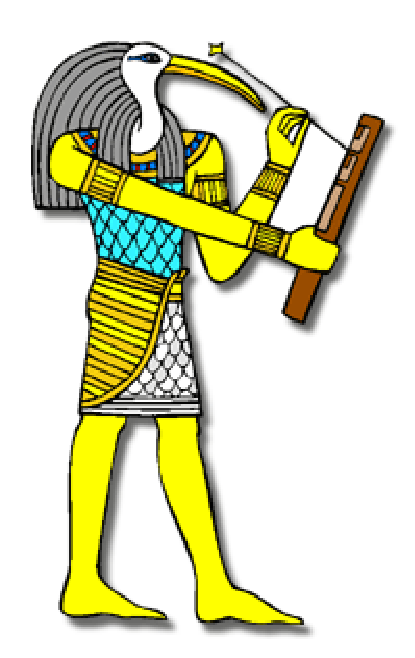
\psfig{file=Egyptthoth.eps}
\fi
\end{figure}

\newpage

\tableofcontents

\newpage

%% Some literature
\nocite{finke:icassp97}
\nocite{finke:asru97}
\nocite{fritsch:icassp96}
\nocite{kemp:eurospeech97}
\nocite{ivica:diss}
\nocite{finke:swb97}
\nocite{soltau:icassp01}
\nocite{soltau:asru2001}


%% =============================================================================
\chapter{Introduction} \label{sec:introduction}
%% =============================================================================

\JaddGloss{JRTk}{The Janus Recognition Toolkit}
\JaddGloss{JANUS}{Equivalent to JRTK, or only the janus binary}
\JaddGloss{Janus}{Equivalent to JRTK, sometimes used for pre-Ibis janus binaries}
\JaddGloss{janus}{The 'janus' binary}
\JaddGloss{Ibis}{The standard one-pass decoder in Janus 5.x.}
\JaddGloss{ISL}{The Interactive Systems Labs at UKA and CMU}
\JaddGloss{UKA}{Universit\"at Karlsruhe (TH)}
\JaddGloss{CMU}{Carnegie Mellon University}

This manual describes \Jgloss{JRTk}, the Janus Recognition Toolkit, in
version  \textsl{V\Jversion},   which    includes  the   \Jgloss{Ibis}
decoder. This manual also contains pointers, where to look for further
information.   One  important  page is  the  online JRTK documentation
available    at   \htmladdnormallink{\texttt{http://isl.ira.uka.de/\~{
}jrtk/janus-doku.html}}{http://isl.ira.uka.de/~jrtk/janus-doku.html}.

In the following chapter \ref{sec:basics}  you'll find the information
you'll need to get Tcl and Janus up and running.  We focus on the UNIX
variants, although much of  the information  also applies for  Windows
installations.  You    might   want to  have  a   look  at    a sample
\Jref{file}{.janusrc} first, which  is the main configuration file for
Janus. The basic concepts of the JANUS user interface are discussed in
\ref{sec:interface}. Chapter \ref{sec:training} covers all you'll need
to   know   in order to  train  a   system using  JRTk,  while chapter
\ref{sec:ibis} covers    the  Ibis decoder.   If   you're experiencing
difficulties and need help in either  installing Janus, configuring it
properly,   or    running  scripts,  the    trouble-shooting   section
\ref{sec:troubleshooting} contains (hopefully) useful information.

The JANUS interface   having  an object-oriented style,    you'll find
descriptions of all modules in chapter \ref{sec:modules}; this will be
of  interest to  both the  user  and the would-be  C  programmer.  The
Tcl-library, which   should save you  a lot   of effort when  building
systems at  script level, is  described in chapter \ref{sec:lib}.  The
``Janus  Scripts Collection'', which   comprises a number  of standard
scripts to build and test systems, also relies  on the Tcl-library. It
is discussed  in section \ref{sec:interface}.  Chapter \ref{sec:files}
describes some of JANUS' files and their formats.

The people  who have worked on   JANUS over the  time can  be found in
\ref{sec:people}.  At  the end of  this document,  you'll also  find a
bibliography and a  glossary.  Chapter \ref{sec:basics}  also contains
some  information on how to use  this manual, available in Postscript,
HTML and  PDF  format. If you  have  questions or problems  with JRTk,
please             send                      e-mail                 to
\htmladdnormallink{\texttt{jrtk@ira.uka.de}}{mailto:jrtk@ira.uka.de}.

Janus was   successfully  used in    a   number of  evaluations,   see
\cite{finke:swb97,soltau:icassp2004,metze:nist2004}.

%\vspace{2cm}
%\ifpdf
%  \centerline{
\includegraphics{janus.png}}
%\else
%  \centerline{
\psfig{file=janus.eps}}
%\fi


%% =============================================================================
\chapter{Basics} \label{sec:basics}
%% =============================================================================

\section{What is it?} \label{basics:whatisit}

The goal of  the ISL's JANUS project  is  to build a  general--purpose
speech     recognition  toolkit   useful    for    both research   and
applications. Currently, the   software  consists of  JRTk,  the Janus
Recognition Toolkit for the development of speech recognition systems,
including  the Ibis  decoder.   This  document attempts to  serve  two
purposes: the  first one is to jump--start  users in getting the basic
jobs done with JANUS,  be it for research  projects, or be it to build
another system using  JANUS, while the second purpose  is to also give
an overview  of the current research  done  within the  JANUS project.
This  document is  for incoming  researchers  and students as  well as
external partners in order to familiarize  themselves with the options
and procedures to make the most of the existing code-base.  At the end
of this document, you find a list of references to JANUS and an index,
covering the most  important  concepts,  files  and commands used   in
JANUS.

\subsection*{Terminology}

Over time, a number of terms have evolved, refering to different parts
of the  system, although  JANUS' nomenclature  is not  always strictly
adhered to:

\begin{description}
\item[JRTk] refers to the ASR Toolkit developed at the \Jgloss{ISL} in
Karlsruhe (\Jgloss{UKA}) and Pittsburgh (\Jgloss{CMU}).
It is implemented in C code, with an interface in Tcl/Tk,
having an object-oriented look-and-feel.
\item[janus] means the \texttt{janus} executable.
\item[JANUS or Janus] can often be replaced by JRTk or janus.
\item[Ibis]  denotes the one-pass decoder available in Janus V5.0 and later.
\end{description}

\subsection*{Why the names?\footnote{From http://concise.britannica.com.}}

\begin{description}
\item[Janus:] Roman god of doorways and archways, after whom the 
    month of January is named.

    Often depicted  as  a  double-faced   head,  he  was  a  deity  of
    beginnings. The worship of Janus dated  back to the earliest years
    of Rome, and the   city had many freestanding  ceremonial gateways
    called  jani,    used for   symbolically auspicious   entrances or
    exits.  The festival of Janus,  the Agonium, took place on January
    9.

\item[Ibis:] Egyptian Djhuty, also spelled Djhowtey.

    In  Egyptian religion,  a  god of   the   moon, of reckoning,   of
    learning, and of  writing.  He  was held   to be the  inventor  of
    writing, the  creator of languages,   the scribe, interpreter, and
    adviser of the gods, and the representative of the sun god, Re.

    Thoth in turn was frequently represented in human form with an
    ibis' head.

\end{description}

\section{About the documentation} \label{basics:doku}

This documentation is intended to cover most  aspects that you'll need
to know to use JRTk at the Tcl/Tk level. You should also find a lot of
useful information  if you need to change  the C-Source.   If you find
errors or   omissions, feel  free  to contact  one of  the maintainers
(section        \ref{sec:people})        or    send        e-mail   to
\htmladdnormallink{\texttt{jrtk@ira.uka.de}}{mailto:jrtk@ira.uka.de}. Don't
forget    to    look    at     the     ``trouble-shooting''    section
\ref{sec:troubleshooting}, too.

% Also,   please  keep the  documentation  up to   date   by writing and
% enhancing sections,  keeping JANUS in a coherent  and tidy state (both
% code  and documentation); think about  the  maintainer's list and  the
% index.

This documentation contains four main parts:

\begin{enumerate}

\item A cookbook of training procedures in chapter \ref{sec:training}. Basic
  system training can most easily be done by using the Janus Scripts Collection
  documented in \ref{janus:scripts}.

\item A How-To on decoding strategies and using existing systems with the 
  Ibis one-pass decoder in chapter \ref{sec:ibis}.

\item The alphabetical list of modules available at Tcl-level with
  their description in chapter \ref{sec:modules}; a list of
  functions provided by the Tcl-library can be found in chapter \ref{sec:lib}.

\item A description of files and formats needed or used in JANUS
  in chapter \ref{sec:files}.

\end{enumerate}


The source and documentation are kept under SVN, it is assumed that you are
familiar with version control. To build documentation from the
sources, you should be able to use ``make pdf'' with the provided
``Makefile'' as follows:

\begin{verbatim}
~/janus/doc > ../src/Linux/janus lib2tex.tcl
~/janus/doc > ../src/Linux/janus tcl2tex.tcl
~/janus/doc > make pdf
\end{verbatim}

Generating documentation was last tested on ``Snow Leopard'' using Tcl 8.4.

%Several output formats are available:

%\begin{description}
%\item[dvi] Simply type ``make'', this is very useful for debugging; if
%  you type ``latex janus-doku'' you should be able to see the error
%  messages generated by \LaTeX.

%\item[ps] This generates a .dvi file and converts it into a .ps
%  booklet which you should be able to print.

%  \textbf{Caveat:} if the back-pages appear upside-down, leave out the pstops
%  command.

%\item[pdf] This creates a .pdf file using pdflatex. This file can be 
%  printed and viewed online and looks much nicer than .html and you
%  have the convenient hyperlinks. Also, after compilation you'll find
%  the file ``link-errors'', which will help you to track wrong and
%  missing hyper-links.

%  \textbf{Caveat:} The .aux files produced by pdflatex are
%  incompatible with the ones from latex. You should therefore always
%  delete them ... (or use ``make clean''). Also, graphics produced by 
%  ``eps2pdf'' didn't look all that great in acroread, so I converted
%  the original data to .png or .jpg, which seems to be fine.

%\item[html] The file janus-doku/janus-doku.html is generated by
%  latex2html and you should be able to view the document with any web-browser.

%  \textbf{Caveat:} The exact formatting depends on the browser and can
%  therefore be rather strange. Also, the inline images used to print
%  formulas etc. have a black border (bottom/ left), if you use the
%  standard version of the script ``pstoimg'' and the ``pnmtools''. You
%  can easily patch ``pstoimg'', it is currently fixed on
%  i13pc33:/usr/bin/pstoimg or look for ``latex2html black border'' or
%  the like on the internet.

%\end{description}

%As of this writing,   it was possible to  generate  reasonably-looking
%documents on  a  Linux  PC running   SuSE 7.2   (keeping in mind   the
%Caveats), however this cannot be guaranteed for all systems. Feel free
%to experiment ...  To write new documentation in \LaTeX, please try to
%match its  look and  feel with existing   files. For your convenience,
%there are a couple of macros which you can use:

%\begin{description}
%\Jitem{$\backslash$Jindex\{object\}} creates a reference to ``object''
%  in the index
%\Jitem{$\backslash$Jlabel\{group\}\{object\}} creates a reference to
%  ``object'' in the index and sets a label for ``group:object'' at the
%  point in text where this command occurs
%\Jitem{$\backslash$Jref\{group\}\{object\}} creates a reference to the
%  corresponding $\backslash$Jlabel command

%  The difference between $\backslash$Jindex and $\backslash$Jref is
%  that $\backslash$Jref creates a reference directly to the text,
%  while $\backslash$Jindex goes into the index

%  The advantage using ``group'' and ``object'' for $\backslash$Jlabel
%  and $\backslash$Jref is that you have one ``object''
%  (e.g. \Jindex{-map}) in the index only once, while you can still
%  have direct links to its occurrence in different ``groups''
%  (e.g. \Jref{module}{CodebookSet} \Jref{CodebookSet}{read} and
%  \Jref{module}{GLat} \Jref{GLat}{read}).
%\Jitem{$\backslash$Jgloss\{ref\}} sets a reference to an entry in the glossary
%\Jitem{$\backslash$JaddGloss\{ref\}\{text\}} describes an entry in the
%  glossary (currently, text can only be one line)
%\Jitem{$\backslash$Jsb\{-Monthy Python\}} is a shortcut to create
%  optional arguments \Jsb{-Monty Python}
%\Jitem{$\backslash$Jitem\{text\}} creates an $\backslash$item$[$text$]$ in the right font and
%  so on
%\end{description}


\section{Installation} \label{basic:installing}

All Janus  software is contained  in a \texttt{janus} directory, which
you can either find  on your distribution  media, copy from somewhere,
or check out from CVS/ SVN. Installing JRTk consists of the following three
steps:

\begin{enumerate}
\item Copy  the janus  distribution  directory somewhere on  your file
system.

We     suggest  to create a  \texttt{janus}    directory  in your home
directory. This directory will be  referred to as \texttt{<JANUSHOME>}
in  the    future,    it  should     contain the     \texttt{library},
\texttt{tcl-lib}, \texttt{gui-tcl} and optionally the    \texttt{bin},
\texttt{src} and \texttt{doc} subdirectories.

\item Set environment variables appropriately.

Set your search path, so  that the correct  janus executable for  your
system and  architecture can be found. On  a Linux system, you can for
example  add  \texttt{<JANUSHOME>/src/Linux.gcc} to your \texttt{PATH}
environment variable. Alternatively, you can copy the executable(s) to
a location already on your search path (e.g. \texttt{\~{ }/bin}).

On Unixes, janus needs three environment variables:

\begin{description}

\Jitem{\Jindex{JANUS\_LIBRARY}} needs to be set to \texttt{<JANUSHOME>/library}
\Jitem{\Jindex{HOST}} should be set to the name of your node. On Linux machines using
a \texttt{tcsh}, you can say \texttt{setenv HOST `uname -n`}
\Jitem{\Jindex{HOME}} should contain the path to your home directory. In principle, this
can be any directory.

\end{description}

Note that on  some Unix machines, it   might also be necessary to  set
\Jindex{TCL\_LIBRARY}  and \Jindex{TK\_LIBRARY}   to appropriate  values
(often \texttt{/usr/lib/tcl8.4} and \texttt{/usr/lib/tk8.4}), and you 
might need to set \texttt{LD\_LIBRARY\_PATH}, if you want to use dynamic 
linking. An example \texttt{.tcshrc} excerpt:

\begin{verbatim}
# JRTk
setenv JANUS_LIBRARY   "${HOME}/janus/library"
setenv TCL_LIBRARY     "/usr/lib/tcl8.4"
setenv TK_LIBRARY      "/usr/lib/tk8.4"
setenv LD_LIBRARY_PATH "${HOME}/tools/nist/lib:${HOME}/tools/portaudio/lib/.libs:${HOME}/tools/libsndfile-1.0.20/src/.libs"
\end{verbatim}

\item Adapt the startup configuration file \Jref{file}{.janusrc} to your needs.

Copy         the    \texttt{<JANUSHOME>/scripts/janusrc}    file    to
\texttt{\$$\{$HOME$\}$/.janusrc}, i.e. the directory declared with the
\texttt{HOME} environment variable. Open the \Jref{file}{.janusrc} file
with a text editor and change the lines setting the \Jindex{JANUSHOME}
variable to    the value of   \texttt{<JANUSHOME>}. If  you experience
difficulties  when creating  logfiles   on  a Windows  platform,   try
uncommenting the \texttt{set LOGFILE "janus.log" } line.

\end{enumerate}

If you  are used to  a  Unix-style environment and   work on a Windows
platform, you    might consider     looking at   the    Cygwin   tools
(\htmladdnormallink{\texttt{http://www.cygwin.com/}}{http://www.cygwin.com/});   although
Janus will run just as well without them.

The default  \Jref{file}{.janusrc}  automatically optimizes your Janus
setup depending on the architecture, operation system and location you
use.  If janus doesn't  start or these automatically detected settings
are incorrect, there are several things you can to check:

  \begin{enumerate}
    \item Are all the dynamically linked libraries there?
      This is not the case if Janus complains about missing libraries, it
      can be fixed by setting the environment variable
      \texttt{LD\_LIBRARY\_PATH} accordingly. Tcl/Tk has to be available
      in the correct version.
    \item Does Janus not start because of wrong X settings? You either
      have to set the \texttt{DISPLAY} environment variable or run a
      Janus binary compiled without X support.
    \item Are the paths set correctly (cf. \texttt{\~{ }/.tcshrc})?
    \item Can Janus initialize properly? The environment variable
      \texttt{JANUS\_LIBRARY} should be set to
      \texttt{\~{ }/janus/library} (or whatever is appropriate)
      and \texttt{\~{ }/.janusrc} should contain the lines 
      \begin{verbatim}
set JANUSLIB  "$env(HOME)/janus/gui-tcl"
set auto_path "$env(HOME)/janus/tcl-lib \
               $JANUSLIB $auto_path"
      \end{verbatim}
      %$
      or equivalent.
      These lines tell Janus where to find the Tcl scripts needed to
      initialize Tcl and Janus itself properly. You can override the
      settings for \texttt{gui-tcl} and \texttt{tcl-lib} in your own
      scripts, but you have to know what you're doing ;-)
    \item If Janus runs all right, but blocks (i.e. stops) when it tries to use
      \texttt{fgets} (which is used in most procedures provided in
      \texttt{tcl-lib}), you're most likely experiencing an
      \texttt{fgets}-Problem and you want to read the \ref{sec:troubleshooting}
      section.

\end{enumerate}

If the   above installation did  not work   for you,  there  are a few
additional  things to check. You'll find   some information in section
\ref{sec:troubleshooting}.

On \texttt{Windows}, JRTk can be installed as follows:

\begin{itemize}
\item install gunzip (GnuWin32) for windows, preferable in version 1.3.5 (gzip-1.3.5-bin.exe)
\item copy .janusrc to your home directory (Documents and Settings/... user name ...)
\item edit .janusrc as appropriate
\item install Tcl8.4 (ActiveTcl8.4.19.1.286921-win32-ix86-threaded.exe)
\item add to system variables (Settings, Control Panel, System, Advanced, Environment Variables):
  \begin{itemize}
  \item new JANUS\_LIBRARY "...path.../janus/library" (Unix notation!)
  \item add to PATH: "...path...$\backslash$GnuWin32$\backslash$bin" and "...path...janus$\backslash$tcl-lib" (you may need to do this as an administrator, Windows notation!)
  \end{itemize}
\item reboot windows
\end{itemize}

Compilation on Windows is usually done with Visual Studio. Also, be aware that
Windows uses CR+LF line endings in text files, which under some circumstances
cannot be read properly on Unixes. Also, if you get weird errors when loading acoustic
models, try if the gzip and gunzip commands can be executed successfully from the command
line.

\section{Language Models} \label{janus:lms}

The generation of language models is not part of JRTk. The standard LM
in the Ibis decoder, created and loaded with

\begin{verbatim}
[LingKS lm$SID NGramLM] load $lmDesc
\end{verbatim}

can read a standard ARPA-format file. These can be created by a number of
toolkits:

\begin{itemize}
\item The CLAUSI tools available at ISL.
\item The CMU-SLMT toolkit, available at 
\htmladdnormallink{\texttt{http://svr-www.eng.cam.ac.uk/\~{ }prc14/toolkit.html}}{http://svr-www.eng.cam.ac.uk/~prc14/toolkit.html}.
\item The SRI Language Modeling Toolkit, available at 
\htmladdnormallink{\texttt{http://www.speech.sri.com/projects/srilm/}}{http://www.speech.sri.com/projects/srilm/}.
\end{itemize}

Which one to use depends on availability and experience. Note that
language models can become very big. Even a compressed (.gz) file will
take up more space on disc and take longer to load than a so-called
language model dump file.


\section{Scoring} \label{basic:scoring}

A  comprehensive scoring  package is  not  part of Janus. Instead, the
Ibis decoder can write hypotheses in CTM format, which can directly be
processed     with NIST's SCLite scoring   package.   Using Tcl, it is
straightforward to write hypos in almost any format you might need.

Additionally, the Tcl-library  implements an ``align'' function, which
you  can  use to  compute string  edit distances for  simple alignment
problems.  See  \Jref{lib}{align.tcl}  for  details.   This file  also
defines a set of lower-level functions, which you might find useful.


\section{Compilation} \label{basic:compiling}

Using  the   Makefile provided  in the \texttt{src}   directory, it is
possible to  compile Janus  on Linux, Mac OS X,   and Solaris.  You can  also set
switches like \texttt{-DMTHREAD}    for a multi-threaded version    of
Janus. Currently, two main targets are supported by this Makefile:

\begin{description}
\item[janus\_opt] the default version, contains everything to train and test
\item[janusNX\_opt] janus\_opt without X-Windows and readline support
\end{description}

Simply  type  \texttt{make}  or  \texttt{make  janus\_opt}  to compile
Janus. On SUNs,   you might  have  to  use \texttt{gmake} instead   of
\texttt{make}.   To build  debugging   or profiling  versions, replace
\texttt{opt} by \texttt{dbg}  or \texttt{prf}. For cleaning the object
directory,    simply  type e.g.      \texttt{make clean\_opt}  for the
optimized  code.  This  is especially neccessary,   when using another
main  target, because  the  object files for   both targets are taking
place in the same directory. Different directories will be created for
\texttt{opt}, \texttt{dbg} and \texttt{prf} version.

Depending  on the exact system configuration   you're using, Janus (on
Unix, particularly Linux) depends on the following libraries:

\begin{description}

\item[System  Librarys]:  \texttt{ld, m, X11}  (until compiled without
X11     support),  \texttt{readline}  (GNU), \texttt{termcap, ncurses,
pthread}

\item[Tcl/Tk 8.0] or greater;  if you  use Tcl/Tk  8.4 or  greater you
should add \texttt{-DUSE\_COMPAT\_CONST} to your \texttt{CFlags}

\item[SPHERE]:     \texttt{sp,    util}  from      NIST's       SPHERE
library\footnote{\htmladdnormallink{\texttt{http://www.nist.gov/speech/tools/sphere\_26atarZ.htm}}{http://www.nist.gov/speech/tools/sphere\_26atarZ.htm},
be warned: the original version  needs modifications to compile  under
modern Linuxes and contains bugs}, if you want to read files in SPHERE
format and you're using \texttt{-DSPHERE}

\end{description}

The exact libraries you'll need depend on  your system and if you want
to use   static   or   dynamic linking. A   complete    description of
compile-time options and  optimizations  is beyond the scope   of this
documentation, on Linux systems we're using the following
switches  for        \texttt{gcc}:         \texttt{-O3     -ffast-math
-fomit-frame-pointer   -march=pentium4},    you   might   also     try
\texttt{-mfpmath=sse -msse} on PIII systems.

The following configurations are well tested:  On SOLARIS machines, we
compile Janus  with the SUN  compiler  WS5.0 and the  GNU compiler gcc
2.95; on Linux we mainly  use the Intel  C++ compiler icc6.0 (7.0) and
gcc 2.95 or greater  (gcc 3.0, 3.2,  3.3).  On Windows  platforms, the
Microsoft compiler  VisualC++ is used. A  work space file can be found
in the \texttt{src/Windows} directory.

If  you want to  generate  a version  which does not  include the three-pass
decoder and the neural net code, do not include \texttt{\$(SEARCHOBS)}
during  compilation  and  don't   include  \texttt{Search\_Init()}  in
\texttt{src/main/janusInit.c}  (use  \texttt{-DIBIS -DNO\_NET}).  This
is accomplished by using the \texttt{ibis\_opt} target.  For a version
which does not rely on Tcl/ Tk, use the \texttt{ibisNTCL\_opt} target.
More information can be  found  in the \texttt{Makefile} available  in
the \texttt{src} directory.


\subsection*{Defines}

Some properties of  the Ibis decoder  can only be changed  by altering
\texttt{\#define}s           and         \texttt{typedef}s          in
\texttt{src/ibis/slimits.h}. Changing these values will require you to
re-compile  Janus and will  also  make it  impossible to re-use object
dump-files, because the internal representation of data structures has
changed.

The most frequently used settings are:

\begin{description}

\item[LVX, LVX\_MAX] sets the maximum language model vocabulary size to
65535 ($2^{16}-1$) or $2^{32}-1$.

\item[SVX, SVX\_MAX] sets the maximum search  vocabulary size to 65535
($2^{16}-1$) or $2^{32}-1$. This setting has to be  at least as big as
the  setting of  \texttt{LVX, LVX\_MAX}.   It  has some  influence  on
runtime memory consumption.

\end{description}


\section{Version history} \label{basic:history}

The version of Janus you are running can be determined from the
start-up message the \texttt{janus} binary displays:

\small{\begin{verbatim}
# ======================================================================
#  ____  ____  _____ _
# |__  ||  _ \|_   _| | _     V5.0 P012 [Nov 11 2002 11:11:11]
#    | || |_| | | | | |/ |  --------------------------------------------
#    | ||  _ <  | | |   <     University of Karlsruhe, Germany
#    | ||_| |_| |_| |_|\_|    Carnegie Mellon University, USA
#   _| | JANUS Recognition
#  \__/        Toolkit        (c) 1993-2002 Interactive Systems Labs
#
# ======================================================================
started janus: on i13pc234.10934, Fri Oct 25 10:03:53 CEST 2002
\end{verbatim}}

This means that this executable was compiled on November 11, 2002. The
version is  ``Janus V5.0, patch-level  12''.  Some versions  of Janus
were ``stamped'' with an  extra tag (e.g.  ``fame'', ``glory'', ...),
which will  then also appear printed  in this line. Also,  CVS or SVN
version information  might be embedded  in the start-up  message. The
last line of output, \texttt{started janus: ...}  is generated in the
file  \Jref{file}{.janusrc}  and  logs  the  start-up  time  of  this
process.  The differences between different versions and patch-levels
of janus are listed below:

\begin{description}

\item[V5.2, P000] released on 2008-??-??

  \begin{itemize}
  \item added various feature enhancement techniques 
  \item incorporates all code written for the RT07S Meeting eval
  \item added description of pre-processing methods to documentation
  \item added ICA
  \end{itemize}

\item[V5.0, P014] released on 2004-09-24

  \begin{itemize}
  \item bugfixes over P013
  \item incorporates all code written for the RT04S Meeting eval
  \item added the description of adaptation methods to documentation
  \item some code for array (pre-)processing integrated
  \item changes in CFG implementation: support of additional grammar
    file formats (FSM, PFSG), support of weight definitions through
    JSGF, support for generating random terminal sequences
  \item support for reading LMs with unsorted n-gram sections, e.g.
    produced by the SRILM-Toolkit
  \item x86-64 code cleaning
  \end{itemize}

\item[V5.0, P013] released on 2003-08-13

  \begin{itemize}
  \item support for training on Windows (bugfixes in IslSystem)
  \item cleaner interface to NGets
  \item incorporates all code written for the RT03 CTS eval
  \item major changes in grammar implementation
  \item discriminative training (MMIE)
  \item bugfixes (splitting of trees, interpolated LMs) 
  \item changed glatComputeGamma and Confidence
  \end{itemize}

\item[V5.0, P012] released on 2002-11-27

  \begin{itemize}
  \item redesigned filler words
  \item code-cleaning for windows
  \end{itemize}

\item[V5.0, P011] released on 2002-10-10

  \begin{description}
  \item[LingKS:] redesign of language model interface (Tcl-scripts
    have to be adapted, see \Jref{proc}{ibisInit} for a comparison
    of the two interfaces). Basically, a language model now is an
    object of type \Jref{module}{LingKS}, while before the language
    model could be of different types (LModelNJD, MetaLM, PhraseLM, CFGSet).
    Now, a language model has a type-specific sub-object. The methods
    and configuration options change accordingly.
  \end{description}

\item[V5.0, P010] released on 2002-02-27

  \begin{description}
  \item[XCM:] option for left context dependency only
  \item[STree:]
    convert search tree representation to general network structure
    and compress the network with the 'coarset partition' algorithm
  \item[GLat:]
    changed lattice generation,
    support to write lattices in HTK format
  \item[LTree:]
    redesigned ltreeFillCtx
    changed acoustic rescoring of lattices
  \item[MetaLM:]
    more efficient interpolation
  \item[PhraseLM:]
    opimized lct handling,
    added reading of map files
  \item[CFG:]
    basic grammar support
  \item[HMM:]
    training of full context dependent single phone words
  \item[Codebooks/Distribs/Senones/Streams:]
    a couple of things
  \end{description}

\item[V5.0, P009] released on 2002-01-07

  \begin{description}
  \item[GLat:]
    \begin{itemize}
    \item changed handling of filler words in forward/backward pass
    \item added ignoreFTag option in glatAlign
    \item improved handling of dis-connected nodes in glatConnect
    \item added nodeN option in glatPrune
    \end{itemize}
  \item[PhraseLM:] fixed lct handling in ScoreArray function
  \item[SMem/STree/SPass:] removed position mapper
  \end{description}

\item[V5.0, P008] released on 2001-12-05

  \begin{itemize}
  \item Changed search space memory management
  \item Fixed trace function in stree
  \item Changes according to the intel compiler
  \end{itemize}

\item[V5.0, P007] released on 2001-11-15

  fixed final (?) problem with deletion of dictionary entries.

\item[V5.0, P006] released on 2001-11-14

  fixed remaining problem with deletion of dictionary entries.

\item[V5.0, P005] released on 2001-11-07

  \begin{itemize}
  \item Increased data size for PHMMX in slimits.h
  \item Added configuration options for svmap and phraseLM
  \item Made praseLM relocatable
  \end{itemize}

\item[V5.0, P004] released on 2001-11-06

  \begin{itemize}
  \item Support for arbitrary HMM-topologies
  \item Added one-state fast match module
  \item Support for streams in scoreA and mladaptS
  \item Deactivated LCT-checker in strace
  \end{itemize}

\item[V5.0, P003] released on 2001-10-30

  Bugfixed and some new features:
  removed a memory allocation bug in the
  semitied covariance code, which showed up under Linux.
  Also made the query of codebooks with distribution names
  working. Made some conversion problems if distribution
  and codebooks have different names.
  Made featureADC a bit more portable.
  Made deletion of words from the dictionary work.
  Added saving to disc of a single distribution or codebook
  into a distributionSet or CodebookSet.

\item[V5.0, P002] released on 2001-10-19

  Update of the windows environment to the IBIS code.

\item[V5.0, P001] released on 2001-10-15

  Established Ibis branch from former Janus main branch jtk-01-01-15-fms.

\end{description}


%% =============================================================================
\chapter{The Janus User Interface} \label{sec:interface}
%% =============================================================================

%% ========================================================================
%%  JANUS-SR   Janus Speech Recognition Toolkit
%%             ------------------------------------------------------------
%%             Object: Basic Tcl
%%             ------------------------------------------------------------
%%
%%  Author  :  Florian Metze & many others
%%  Module  :  basicTcl.tex
%%  Date    :  $Id: basicTcl.tex 2390 2003-08-14 11:20:32Z fuegen $
%%
%%  Remarks :  
%%
%% ========================================================================
%%
%%  $Log$
%%  Revision 1.2  2003/08/14 11:18:44  fuegen
%%  Merged changes on branch jtk-01-01-15-fms (jaguar -> ibis-013)
%%
%%  Revision 1.1.2.4  2002/11/21 16:15:45  metze
%%  Pre-P012
%%
%%  Revision 1.1.2.3  2002/11/20 16:12:12  metze
%%  Doku Pre-P012
%%
%%  Revision 1.1.2.2  2002/08/26 16:40:37  metze
%%  Re-organization of modules
%%
%%  Revision 1.1.2.1  2002/08/01 13:42:20  metze
%%  Fixes for clean documentation.
%%
%% ========================================================================

\section{Tcl basics in 5 minutes}

Tcl stands for 'tool command language' and is pronounced 'tickle.'

\subsection*{Starting}

You start tcl by typing  \texttt{tcl}  or \texttt{tclsh} in your  Unix
shell. Thus  you enter an interactive mode  within Tcl.  You can leave
with the tcl  command \texttt{exit}. If you  want to use the  tcl tool
kit (TclTk) you use \texttt{wish} instead of \texttt{tcl}.

\begin{verbatim}
> tcl
tcl> # this is a comment because the line starts with '#'
tcl> # now we define the variable text
tcl> set text "hello world"
tcl> puts $text
hello world
tcl> exit
>
\end{verbatim}

%% $

\subsection*{Variables}

Variables in tcl can be defined with the  command \texttt{set} and the
value can be     used with \texttt{\$variable\_name}.  Arrays can   be
indexed with arbitrary names in (). Curly  braces are used to separate
variable names from following characters.

\begin{verbatim}
tcl> set name1 Hans
tcl> puts $name1
Hans
tcl> set name2 $name1
tcl> puts ${name2}_im_Glueck
Hans_im_Glueck
tcl> set data(name) Hans
tcl> set data(age)  35
tcl> set data(1,2)  something
tcl> set index name
tcl> puts $data($index)
Hans
\end{verbatim}

%% $

\subsection*{Commands, grouping and procedures}
 
Commands and procedures are called with their name followed by
arguments. Arguments are separated by spaces. They can be grouped
together with "" or {}. The difference is that variables within "" will
be replaced. ';' separates commands in one line.

\begin{verbatim}
tcl> set a 1
tcl> puts "$a + 1"
1 + 1
tcl> puts {$a + 1}
$a + 1
tcl> puts "{$a} + 1"
{1} + 1
tcl> set b 1; puts $b;     # bla bla
\end{verbatim}

A command and arguments within [] will be executed and [command arg1
arg2 ..] will be replaced with the return value.

\begin{verbatim}
tcl> expr 1 + 2
3
tcl> puts "1 + 2 = [expr 1 + 2]"
1 + 2 = 3
\end{verbatim}

%% $

The interpretation of \$variable and [] can be switched off with \\.

\begin{verbatim}
tcl> set a 999
tcl> puts "\[$a \$\]"
[999 $]
tcl> puts {[$a $]}
[$a $]
\end{verbatim}

New  commands or better   procedures can be   defined with the command
\texttt{proc}.

\begin{verbatim}
tcl> proc add {a b} {return [expr $a + $b]}
tcl> add 1 2
3
\end{verbatim}

Note that the procedure name 'add', the variable list '{a b}' and the
body of the function '{return [expr \$a + \$b]}' are the arguments of the
command 'proc'. You can also use optional arguments with their default
value.

\begin{verbatim}
tcl> proc printText {times {text "hello word"}} {
=>     for {set i 0} {$i<$times} {incr i} {
=>       puts $text
=>     }
=>     return $times
=>   }
tcl> printText 2
hello word
hello word
tcl> printText 1 "hello Monika"
hello Monika
\end{verbatim}

Each procedure has a local scope for variables. But you can use the
'global' command in a procedure to access global variables.

\begin{verbatim}
tcl> proc putsnames {} {global name1; puts $name1; puts $name2}
tcl> putsnames
can't read "name1": no such variable
tcl> set name1 Tanja
tcl> set name2 Petra
tcl> putsnames
Tanja
can't read "name2": no such variable
\end{verbatim}

\subsection*{Control flow}

\begin{verbatim}
tcl> if {$i > 0} {puts "1"} else {puts "0"}
tcl> if {"$name" == "Tilo"} {
=>     #
=>     #do something here
=>     #
=>   }
tcl> for {set i 0} {$i < 10} {incr i} {puts $i}
tcl> foreach value {1 2 3 5} {puts stdout "$value"}
tcl> while {$i>0} {incr i -1}
tcl> switch $i {
=>     1         {puts "i = 1"}
=>     "hello"   {puts "hi"}
=>     default   {puts "?"}
=>   }
\end{verbatim}

%% $

You can exit a loop with 'break' or 'continue' with the next iteration.

\subsection*{Errors}

With 'catch' errors can be trapped.

\begin{verbatim}
tcl> if [catch {expr 1.0 / $a} result ] {
=>      puts stderr $result
=>   } else {
=>      puts "1 / $a = $result"
=>   }       
\end{verbatim}

\subsection*{File I/O}

\begin{verbatim}
tcl>  set FP [open $fileName r]
tcl>  set found 0
tcl>  while {[gets $FP line] >= 0} {
=>       if {[string compare "ABC" $line] == 0} {set found 1; break}
            # found exactly "ABC"
=>       if ![string compare "XYZ" $line] {set found 2; break}
            # found exactly "XYZ"
=>       if [string match ABC*XYZ $line] {set found 3; break}
            # found "ABC..something..XYZ"
=>    }
tcl>  close $FPI

tcl>  set FP [open $fileName r]
tcl>  set first100bytes  [read $FP 100] 
tcl>  set rest           [read $FP]
tcl>  close $FPI
\end{verbatim}

\subsection*{The string command}

Strings are the basic data items in Tcl. The general syntax of the Tcl
\texttt{string} command is

\texttt{string /operation stringvalue otherargs/}.

\begin{verbatim}
tcl> string length abc
3
tcl> string index abc 1
b
tcl> string range abcd 1 end
bcd
\end{verbatim}

To compare two strings  you can also  use \texttt{==}. But  that might
not work as you wanted with strings containing digits because 1 equals
1.00 (but not in a string sense).

\begin{verbatim}
     if ![string compare $a $b] {puts "$a and $b differ"} 
\end{verbatim}

Use 'first' or 'last' to look for a substring. The return value is the
index of the first character of the substring within the string.

\begin{verbatim}
tcl> string first abc xxxabcxxxabcxx
3
tcl> string last abc xxxabcxxxabcxxx
9
tcl> string last abc xxxxxx
-1
\end{verbatim}

The 'string match' command uses the glob-style pattern matching like
many UNIX shell commands do (Glob-style syntax):

\begin{description}
\item[*] Matches any number of any character.
\item[?] Matches any single character.
\item[[ ]] One of a set of characters like [a-z].
\end{description}

\begin{verbatim}
tcl> string match {a[0-9]bc?def\?ghi*} a5bcYdef?ghixxx
1

tcl> set a [string tolower abcXY]
abcxy
tcl> string toupper $a
ABCXY
tcl> string trim "  abc  "
abc
tcl> string trimright "xxabcxxxx" x
xxabc
tcl> string trimleft "  a  bc" 
a  bc
\end{verbatim}

Here comes a small example that finds the word with 'x' in a sentence.

\begin{verbatim}
tcl> set s {abc dexfgh ijklm}
tcl> string first x $s
6
tcl> set start  [string wordstart $s 6]  ;# start position
4 
tcl> set end    [string wordend $s 6]    ;# position after word
10 
tcl> string range $s $start [expr $end - 1]
dexfgh
\end{verbatim}

\subsection*{More commands dealing with strings}

\begin{verbatim}
tcl> set a abc
tcl> append a def
abcdef

tcl> puts [format "%8s\t%8.4f" $a -12.7]
  abcdef        -12.7000
tcl> scan "distance 12.34m" "%s%f%c" what value unit
3 
\end{verbatim}

\subsection*{Regular Expressions}

Regular expression syntax. Matches any character.

\begin{description}
\item[*] Matches zero or more.
\item[?] Matches zero or one.
\item[( )] Groups a sub-pattern.
\item[|] Alternation.
\item[[ ]] Set of characters like [a-z]. [\^0-9] means that numbers are excluded.
\item[\^\_] Beginning of the string.
\item[\$] End of string.
\end{description}

\begin{verbatim}
tcl> regexp {hello|Hello} Hello
1
tcl> regexp {[hH]ello} Hello
1
tcl> regexp {[0-9]\.([a-z])([a-wyz]*)} "xxx8.babcxxxxxx" match s1 s2
1
tcl> puts "$match $s1 $s2"
8.babc b abc

tcl> regsub {[0-9]\.([a-z])([a-wyz]*)} "xxx8.babcxxxxxx" {__\1__\2__&__}  var
tcl> puts $var
xxx__b__abc__8.babc__xxxxxx
\end{verbatim}

\subsection*{Lists}

Tcl lists are just strings with a special interpretation. Separated by
white space or grouped with braces or quotes.

\begin{verbatim}
tcl> set mylist "a b {c d}"
tcl> set mylist [list a b {c d}]         ;# same as above
tcl> foreach element $mylist {puts $element}
a
b
c d
\end{verbatim}

Here several Tcl commands related to lists:

\begin{verbatim}
tcl> lindex $mylist 1         ;# note the index starts with 0
b
tcl> llength $mylist          ;# 'c d' is only one element
3

tcl> lappend mylist {g h}     ;# this time the list name 'mylist' is used
a b {c d} {g h}
tcl> lrange $mylist 2 end
{c d} {g h}
tcl> linsert $mylist 3 E x    ;# note that we don't give the list name here!
a b {c d} E x {g h}
tcl> set mylist [linsert $mylist 3 E x];# to change the list we have to use 'set'
a b {c d} E x {g h}

tcl> lsearch -exact $mylist E ;# other modes are the default '-glob' and '-regexp'
3
tcl> lreplace $mylist 3 5 e f {g h i} 
a b {c d} e f {g h i}
tcl> lreplace $mylist 3 3     ;# delete element 3

tcl> lsort "-1.2 -1 -900 -90 1e-3 10"
-1 -1.2 -90 -900 10 1e-3
tcl> lsort -real "-1.2 -1 -900 -90 1e-3 10"
     # other flags are '-ascii','-integer','-increasing','-decreasing'
-900 -90 -1.2 -1 1e-3 10

tcl> list "a b" c
{a b} c
tcl> concat "a b" c
a b c

tcl> join "{} usr local bin" /
/usr/local/bin
tcl> split /usr/my-local/bin /-
{} usr my local bin
\end{verbatim}

\subsection*{Arrays}

\begin{verbatim}
tcl> array exists a
0
tcl> set a(0) 0.12;   set a(1) 1.23;   set a(name) hello  

tcl> array size a
3
tcl> array names a
0 name 1
tcl> array get a 
0 0.12 name hello 1 1.23
\end{verbatim}

The initialization could have been done with:

\begin{verbatim}
tcl> array set a "0 0.12 name hello 1 1.23"
tcl> array set b [array get a]     ;# Copy array b from a:
\end{verbatim}

Other array commands are startsearch, nextelement, anymore,
donesearch.

%%% Local Variables: 
%%% mode: plain-tex
%%% TeX-master: t
%%% TeX-master: "janus-doku"
%%% End: 

%% ========================================================================
%%  JANUS-SR   Janus Speech Recognition Toolkit
%%             ------------------------------------------------------------
%%             Object: Basic Janus UI
%%             ------------------------------------------------------------
%%
%%  Author  :  Florian Metze & many others
%%  Module  :  basicJanus.tex
%%  Date    :  $Id: basicJanus.tex 2390 2003-08-14 11:20:32Z fuegen $
%%
%%  Remarks :  
%%
%% ========================================================================
%%
%%  $Log$
%%  Revision 1.2  2003/08/14 11:18:44  fuegen
%%  Merged changes on branch jtk-01-01-15-fms (jaguar -> ibis-013)
%%
%%  Revision 1.1.2.2  2002/08/26 16:40:37  metze
%%  Re-organization of modules
%%
%%  Revision 1.1.2.1  2002/08/01 13:42:20  metze
%%  Fixes for clean documentation.
%%
%% ========================================================================

\section{Janus Objects}

JANUS was designed to be programmable. The programming language is
Tcl/Tk, expanded by some object classes and their methods. Object
classes are things like dictionaries, codebooks, but also the decoder
itself is an object class. Every object class has its methods
(operations that can be done with objects of that class). Objects can
have subobjects and can be hierarchically organized. The object oriented
programming paradign allows, at least in principle, to plug in and out
objects as one wishes. Simply change the dictionary by assigning a new
one, copy codebooks as easily as "cb1 := cb2", add distribution
accumulators as easily as "ds1.accu += ds2.accu", etc.

\subsection*{Create JANUS Objects}

Objects are meant to hold data but also provide methods to manipulate
that data. To define an object you have to specify its *type*. The
convention is that type names start with capital letters and objects
with small letters. You can define as many objects of one type as you
like. To see what types exist just type (one of the few) JANUS command
'types'.\footnote{By the way '\%' is the prompt of the JANUS shell.
 You can also use any Tcl and Tk commands.}

\begin{verbatim}
% types
FlatFwd ModelArray DurationSet Word Cbcfg SampleSet DVector PTree HMM 
Vocab FMatrix CodebookMapItem PTreeSet MLNorm Dscfg PathItemList 
CodebookAccu HypoList DBaseIdx SampleSetClass SenoneTag Feature 
PhonesSet DCovMatrix Phone FBMatrix Phones DistribAccu IMatrix 
TopoSet SVector XWModel IArray DMatrix FVector StateGraph FCovMatrix 
Duration PTreeNode LatNode Hypo Senone TreeFwd LDA Topo MLNormClass 
Codebook Tags LDAClass FeatureSet Tree PhoneGraph CodebookMap Path 
Search AModelSet RewriteSet
\end{verbatim}

The list you get here depends on the version and compile options. You
create an object when you enter a *type name* followed by the *name of
the new object*. Some types require additional arguments, like
subobjects. As an example we define an object (let's call it 'ps') of
type PhonesSet. You can get a list of all objects you have defined with
the command 'objects'. One object name can only be used once (also for
different types) but you can 'destroy' objects. 'destroy' is a standard
method of every object (s.b.).

\begin{verbatim}
% PhonesSet ps
ps
% PhonesSet ps
WARNING itf.c(0287)   Object ps already exists.
% PhonesSet ps2 
ps2
% objects
ps ps2
\end{verbatim}

summary: JANUS commands *types * list all object types
*objects * list all objects defined by user

\subsection*{Standard Methods}

As soon as you have defined an object you can use its *name* followed by
a *method* and arguments. The different object types have their own
methods of course but at least a few are standard methods that exist for
every object. These are

\begin{description}
\item[type] gives the type of the object
\item[puts] print contents of the object
\item[configure] configure the object
\item[:] allow access to list element
\item[.] allow access to subobjects
\item[destroy] destroy object
\end{description}

To find out what other methods exist we enter eather the *type name*
without any object name or the object name follwed by '-help'. To get
more information about a specific method we enter the object name, the
method and '-help'.

\begin{verbatim}
% ps -help

DESCRIPTION

A 'PhonesSet' object is a set of 'Phones' objects.

METHODS

puts               displays the contents of a set of phone-sets
add                add new phone-set to a set of phones-set
delete             delete phone-set(s) from a set of phone-sets
read               read a set of phone-sets from a file
write              write a set of phone-sets into a file
index              return index of named phone-set(s)
name               return the name of indexed phone-set(s)

% ps add -help
Options of 'add' are:
 < name>    name of list (string:"NULL")
 < phone*>  list of phones
% ps add VOWEL A E I O U
\end{verbatim}

We just added the element 'VOWEL' to the PhonesSet object ps. To see the
contents of the object we can use the method 'puts' or just the object
name which is the same in most cases.

\begin{verbatim}
% ps puts 
VOWEL
% ps
VOWEL
\end{verbatim}

\subsection*{Access to Elements and Subobjects}

The standard methods ':' and '.' allow access to elements and subobjects
respectively. *Elements* of an objects have the same kind of structure
like the words of a dictionary or phone groups (like the 'VOWEL') in the
PhonesSet. Nevertheless they can also be objects and most time they are.
*Subobjects* are more unique, like the Phones of a dictionary as we will
see immedeately. For these two methods and only for them you can omit
the spaces between the object and also between the single argument which
is the name of the element or the subobject. If you don't give a name
you will obtain a list of the choices.\footnote{In case of ':' you again 
get a list of the elements like with 'puts' or just the object name with 
no method.}

\begin{verbatim}
% ps:
VOWEL
% ps:VOWEL
A E I O U
% ps type
PhonesSet
% ps:VOWEL type
Phones
\end{verbatim}

Let's assume we have also defined a phone group 'PHONES' in the
PhonesSet 'ps' that contains all the Phones of a dictionary. Then we can
create a dictionary object that needs the name of a *Phones object* and
of a *Tags object* as arguments. Both have to be created before.

\begin{verbatim}
% Tags ts
ts
% Dictionary d ps:PHONES ts
d
% d add DOG "D O G"
% d add DUCK "D U CK"
% d.
phones tags item(0..1) list
% d:
DOG DUCK
\end{verbatim}

With 'd.phones' for example you have access to the object 'ps:PHONES'.
Although there is a method for PhonesSet to delete elements like
'PHONES' you will get an error if you try that because it was locked as
you defined the dictionary. This prevents objects from being deleted
while they are used by other objects.

\subsection*{Configuration}

Sometimes it might be necessary to configure *objects* or *object
types*. You can get all configure items, get a specific one or set one
or more items. In the latter case only if they are writable.

\begin{verbatim}
% ps configure
{-useN 1} {-commentChar {;}} {-itemN 2} {-blkSize 20} 
% ps configure -commentChar
{;}
% ps configure -commentChar #
\end{verbatim}

Note: The old comment sign ';' was protected with curly braces {}
because it is the command separator in Tcl.

Can you explain the following line and its return value.

\begin{verbatim}
% ps configure -commentChar ;
#
\end{verbatim}

%%% Local Variables: 
%%% mode: latex
%%% TeX-master: t
%%% End: 

%% ========================================================================
%%  JANUS-SR   Janus Speech Recognition Toolkit
%%             ------------------------------------------------------------
%%             Object: Documentation for Script Collection
%%             ------------------------------------------------------------
%%
%%  Author  :  Florian Metze & many others
%%  Module  :  scriptCollection.tex
%%  Date    :  $Id: scriptCollection.tex 2568 2004-11-09 19:54:57Z metze $
%%
%%  Remarks :
%%
%% ========================================================================
%%
%%   $Log$
%%   Revision 1.4  2004/11/09 19:53:48  metze
%%   *** empty log message ***
%%
%%   Revision 1.3  2004/08/16 16:10:13  metze
%%   Additions for P014 by Florian
%%
%%   Revision 1.2  2003/08/14 11:18:56  fuegen
%%   Merged changes on branch jtk-01-01-15-fms (jaguar -> ibis-013)
%%
%%   Revision 1.1.2.7  2003/08/07 13:01:24  metze
%%   *** empty log message ***
%%
%%   Revision 1.1.2.6  2003/04/30 15:43:59  metze
%%   Changes before the new repository
%%
%%   Revision 1.1.2.5  2002/11/21 16:15:46  metze
%%   Pre-P012
%%
%%   Revision 1.1.2.4  2002/11/05 13:43:49  soltau
%%   typo
%%
%%   Revision 1.1.2.3  2002/11/05 07:45:44  metze
%%   Removed reference to trainPT
%%
%%   Revision 1.1.2.2  2002/10/04 13:30:29  metze
%%   More docu
%%
%%   Revision 1.1.2.1  2002/08/26 16:40:37  metze
%%   Re-organization of modules
%%
%%
%% ========================================================================


\section{The Janus Library: ``tcl-lib'' and ``gui-tcl''}

The Tcl-library is  a set of procedures  the user can invoke and which
provide  a number of ``convenience''  functions.   The scripts in  the
Janus  Scripts Collection  (\texttt{\~{ }/janus/scripts},  see chapter
\Jref{janus}{scripts})  use      the    Tcl-library extensively.   The
Tcl-library   can  be   found   in   \texttt{\~{ }/janus/tcl-lib}  and
\texttt{\~{ }/janus/gui-tcl}.   To  auto-load   the  functions,  the
Tcl-variable \texttt{auto\_path} has to be set correctly, i.e.  to the
value of these two directories. Also, a  file \texttt{tclIndex} has to
exist   in these directories. You  should  not need to   worry, if you
follow  the standard install instructions,  otherwise refer to any Tcl
manual for a description of the auto-loading mechanism.  The functions
available in the tcl-lib are described in chapter \Jref{sec}{lib}.

\section{The Janus Scripts Collection} \label{janus:scripts}

The  directory  \texttt{\~{ }/janus/scripts}  contains  a  number  of
scripts, which   we  normally use  to train  and   test systems. These
scripts  are  often modified and    copied in a  system  directory for
documentation purposes.

If you have access to an example system  (i.e. IslData, IslSystem), we
suggest that  you have a  look at it  to see how  data and scripts are
typically  organized in a  JRTk project.  Usually,  the structure of a
project  looks as  follows (this  project  would be called the  ``M1''
system):

{\small
\begin{verbatim}
M1/
|
+--master.log
|
+--Log/
|  '--makeCI.log
|    
+--desc/
|  +--desc.tcl
|  +--codebookSet
|  +--distribSet
|  +--distribTree
|  +--featAccess
|  +--featDesc
|  +--phonesSet
|  +--tags
|  +--tmSet
|  +--topoSet
|  '--topoTree
|
+--train/
|  +--ldaM1.bmat
|  +--ldaM1.counts
|  +--convList
|  |
|  +--Log/
|  |  +--lda.log
|  |  +--samples.log
|  |  +--kmeans.log
|  |  '--train.log
|  |
|  +--Accus/
|  |  +- 1.cba.gz
|  |  '--1.dsa.gz
|  |
|  '--Weights
|     +--0.cbs.gz
|     '--0.dss.gz
|
+--test/
   +--convList
   |
   +--Log/
   |  '--test.log
   |
   '--hypos/
      '--H_kottan_z26_p0_LV.ctm
\end{verbatim}
}

Typically, a  system  directory (here:  ``M1'')  contains a number  of
sub-directories, each  for  different phases (label  writing, cepstral
mean computation,  model  training (``train''),   polyphone  training/
clustering, testing (``test''), ...). Each directory then contains the
data resulting from this step and log-files.

The   scripts   who   perform   the  operations   can   be left  under
\texttt{janus/scripts}, only \texttt{desc.tcl} is a configuration file
specific to  this project  and  is therefore copied into  the  project
directory along with the other description files.

\subsection{Available Scripts}

The following scripts are available in the Janus Scripts Collection
(in the order in which they are usually called):

\begin{description}

\Jitem{genDBase.tcl} \label{janus:genDBase.tcl}

  This script can be used to create a database, which is necessary for
  all further steps.  Look at the resulting  database files (they  are
  called \texttt{db-\{spk|utt\}.\{idx|dat\}} to see what   information
  can and needs to be defined in the database.

  Depending on your needs  and   the format, in   which you  have  the
  information  available, you will need  to modify this script to suit
  your needs.

\Jitem{makeCI.tcl}    \label{janus:makeCI.tcl}

  Creates the following description files for a context-independent
  (CI) system:

  \begin{itemize}
    \item codebookSet
    \item distribSet
    \item distribTree
  \end{itemize}
  
  You'll need to have all the other description files in place, namely
  the phonesSet. If you want to use a different architecture
  (i.e. semi-tied, or non-tri-state architectures), you can edit this
  file according to your needs.

\Jitem{means.tcl}     \label{janus:means.tcl}

  This script will create the cepstral means needed for the standard
  pre-processing of the Janus-based recognizers.

\Jitem{lda.tcl}       \label{janus:lda.tcl}

  This script computes an LDA matrix, used for the standard
  pre-processing.

\Jitem{samples.tcl}   \label{janus:samples.tcl}

  This script extracts samples for further clustering with \Jref{janus}{kmeans.tcl}.

\Jitem{kmeans.tcl}    \label{janus:kmeans.tcl}

  Performs KMeans clustering on data extracted with \Jref{janus}{samples.tcl}.

\Jitem{train.tcl}     \label{janus:train.tcl}

  Performs EM-training on initial codebooks from \Jref{janus}{kmeans.tcl}.
  Can be used for training of a context-independent (CI),
  a context-dependent (CD), or a polyphone (PT) system.
  Normally, we do label training although it is also possible
  to do viterbi- or forward-backward-training by replacing
  \Jref{proc}{viterbiUtterance} by for example \Jref{proc}{viterbiUtterance}.

\Jitem{makePT.tcl}    \label{janus:makePT.tcl}

  Creates a polyphone (PT) system from the CI description files.

\Jitem{cluster.tcl}   \label{janus:cluster.tcl}

  Clusters the contexts from PT training.

\Jitem{split.tcl}     \label{janus:split.tcl}

  Creates the context-dependent (CD) models after PT training, creates
  the following CD description files (with $N > 0$):

  \begin{itemize}
    \item codebookSet.N.gz
    \item distribSet.Np.gz
    \item distribTree.Np.gz
  \end{itemize}

\Jitem{createBBI.tcl} \label{janus:createBBI.tcl}

  Creates a BBI (bucket-box intersection) tree for a codebook.

\Jitem{test.tcl}      \label{janus:test.tcl}

  Tests a system.

\Jitem{score.tcl}     \label{janus:score.tcl}
  
  Scores a system, i.e. computes word error rates.

\Jitem{ana\_time.tcl}  \label{janus:anatime.tcl}

  Allows to  measure the CPU-time  spent in  pre-defined sections of a
  script. You can find more details about timing analysis and how to use
  this script in section \ref{ibis:timing}.

\Jitem{labels.tcl}    \label{janus:labels.tcl}

  Writes new labels with an existing system. Can also be used to
  bootstrap a new system using the acoustic models from another system.

\end{description}

An example  \texttt{desc.tcl}  file  is also  included in  the  script
collection.  All  ``working'' scripts source \texttt{../desc/desc.tcl}
and load the settings (paths, ...)  from there,  although these can be
overridden   at       the   command line        or   in   the   script
themself. \texttt{janusrc} is an example configuration file for janus,
which  is  best  adapted   and copied   into your home    directory as
\texttt{.janusrc}.

\subsection{Working with master.tcl} \label{janus:master.tcl}

We  assume  you have  a  system directory   setup correctly, including
pre-computed   time-alignments   (``labels''). When  working with  the
example system ``IslSystem'', you have a \texttt{desc} directory which
contains  an appropriate  \Jref{file}{desc.tcl}  file. In the ``system
home directory'' (``M1'' in the above example), you can now enter

\begin{verbatim}
janus <janus>/scripts/master.tcl -do init means lda samples kmeans train
\end{verbatim} 

and the master script will create a context-independent (CI) system in
the \texttt{M1/train}  directory.  \texttt{$<$janus$>$} refers to your
Janus  installation     directory.\footnote{Usually   this   will   be
\texttt{\~{ }/janus}.}   You'll find    logfiles  in   your system's
\texttt{Log}   subdirectory.    The following  steps  were  performed,
calling the following scripts:

\begin{enumerate}
\item[init] (\Jref{janus}{makeCI.tcl})
  to create the codebookSet, distribSet, distribTree definition files
  for the CI system

\item[means] (\Jref{janus}{means.tcl})
  to compute the cepstral means for this preprocessing. This can be
  re-used for a CD-system

\item[lda] (\Jref{janus}{lda.tcl})
  to compute the LDA (Linear Discriminant Analysis) matrix for this
  system.

\item[samples] (\Jref{janus}{samples.tcl})
  to extract samples for the CI models

\item[kmeans] (\Jref{janus}{kmeans.tcl})
  to create initial codebooks from the samples, written into {\tt Weights/0}.
  Once this step is completed, you can remove the {\tt data} subdirectory.

\item[train] (\Jref{janus}{train.tcl})
  to perform several iterations of EM-training on the initial codebooks.
  At the end of this step, you can remove the contents of the {\tt Accus}
  subdirectory as well as intermediate codebooks in {\tt Weights}, to save
  space.

\end{enumerate}

\Jref{janus}{master.tcl} will show you the  command lines it executes,
if you want   to parallelize your  training, you  can copy  the output
lines   {\tt exec  janus lda.tcl   ...} (omitting  the  {\tt exec} and
changing the   log  file name) and  run   the same  script  on several
machines.

To run the polyphone training, enter

\begin{verbatim}
janus <janus>/scripts/master.tcl -do makePT trainPT cluster split
\end{verbatim}

This will create the description files for a context-dependent system.

To run the training for the context-dependent system, enter

\begin{verbatim}
janus <janus>/scripts/master.tcl -do lda samples kmeans train test score
\end{verbatim}

assuming  that you have created  a new directory  and set up the paths
for codebookSetParam and distribSetParam accordingly. To create initial
time alignments for a new system, edit the description file (probably
you'll have to change most of the files usually in the ``desc'' directory
to match your old system and your desired new setup) and execute:

\begin{verbatim}
janus <janus>/scripts/master.tcl -do labels
\end{verbatim}

If you type

\begin{verbatim}
janus <janus>/scripts/master.tcl -h
\end{verbatim}

you'll get a list of all command line options for \texttt{master.tcl}.

\subsection{Extra scripts} \label{janus:extrascripts}

The   \texttt{scripts} directory  also  contains a  number of scripts,
which    can       not     (currently)    be       called      through
\Jref{janus}{master.tcl}. They  can however  serve as  example scripts,
which can be adapted to specific problems.

\begin{description}

\Jitem{map.tcl} \label{janus:map.tcl}

An example script to perform \Jgloss{MAP} adaptation.

\Jitem{mllr.tcl} \label{janus:mllr.tcl}

An example script to perform \Jgloss{MLLR} adaptation.

\end{description}

%%% Local Variables: 
%%% mode: latex
%%% TeX-master: t
%%% End: 


%% =============================================================================
\chapter{Pre-Processing with JRTk} \label{sec:frontend}
%% =============================================================================


Janus  can use just about  any  conceivable recognizer front-end. Most
``standard'' ways of doing pre-processing, such as mel frequency cepstral coefficients (MFCC)s or perceptual linear prediction, are almost certainly already implemented    in the  \Jref{module}{FeatureSet}.  FIR-Filters   can be
applied to features with the  \Jref{FeatureSet}{filter} method, and so
on. Have   a  look   at  the   \Jref{module}{FeatureSet}  and  example
\Jref{file}{featDesc}s to see what's already available. In the remainder of this chapter we will give more details about some of the features which are available in the \Jref{module}{FeatureSet} module and might require a more detailed explanation.

Various sample scripts including MFCC and warped-minimum variance distortionless response (MVDR) front-ends as well as reverberation compensation by multi-step linear prediction (MSLP), non-stationary noise compensation by particle filter (PF)s and joint compensation of both distortions can be found in the scripts directory.

\section{Spectral Estimation} \label{janus:specest}

Spectral analysis is a fundamental part of speech feature extraction for automatic recognition and many other speech processing algorithms. Janus contains a broad variety of spectral estimation techniques to adjust for spectral resolution, variance of the estimated spectra, and to model the frequency response function of the vocal tract during voiced speech. In the following example the Fourier spectrum $<$FFT$>$, the warped MVDR spectral envelope $<$MVDR$>$ ---mel frequency for a 16 kHz signal--- and the scaling of the spectral envelope $<$sMVDR$>$ is demonstrated:

\begin{verbatim}
set order 30
set windowsize 16ms

$fes spectrum  FFT    ADC         $windowsize
$fes adc2spec  ADC                $windowsize -win hamming -adc SPADC
$fes specest   MVDR   SPADC       $order -type MVDR \
                                         -lpmethod warp -warp 0.4595
$fes specadj   sMVDR  MVDR   FFT  -smooth 2
\end{verbatim}

\noindent
NOTE: For a 8 kHz signal the warp factor has to be replaced by 0.3624.

~ \\

Different spectral estimation techniques within the Janus framework are compared and explained in~\cite{Wolfel2005b,Wolfel2006,Wiley}.

\section{VTLN} \label{janus:vtln}

Vocal track length normalization (VTLN) can be applied either in the linear or in the warped (mel) domain. The domain mainly depends on the used spectral estimation method as described in section~\ref{janus:specest}. While the implementation in the linear domain is not able to reduce the number of spectral bins (can for example be implemented by the mel filterbank), the implementation in the warped domain can provide a reduced number of spectral bins. The two different implementations can be called as follows:

\begin{itemize}
	\item In the linear domain
\begin{verbatim}
$fes   VTLN <TO> <FROM> $WARP -mod lin -edge 0.8
\end{verbatim}

	\item In the warped (mel) domain
\begin{verbatim}
set warp [expr round(200-$WARP*100)/100.0]

if { $warp < 0.75 } { set warp 0.75 }
if { $warp == 1.0 } { set warp 1 }   
if { $warp > 1.35 } { set warp 1.35 }

if {[llength [objects FBMatrix VTLN${warp}]] != 1} {
    writeLog stderr "LOAD filterbank 16 kHz, 16 ms, 129 bins, \
        ${warp} warp"
    source ${path}/filterbanks/Filterbanks16kHz16ms129bins/ \
        VTLN.filterbank.${warp}
}
 
$fes   filterbank <TO> <FROM> VTLN${warp}
\end{verbatim}

NOTE: Different pre-calculated filterbank can be loaded for 8 and 16 kHz. 

\end{itemize}

\section{Feature Enhancement} \label{janus:enhancement}

To cope well with the non-stationary behavior of additive and convolutive distortions Janus contains different feature enhancement techniques which can be used in addition to other adaptation methods as described in section~\ref{janus:adaptation}. In the remainder of this section we present a generic compensation framework to jointly compensate for additive and reverberant distortion. The framework can be easily adjusted to compensate for additive or reverberant distortion only as will be discussed.

Different feature enhancement techniques within the Janus framework are compared and explained in~\cite{Wolfel2008e,Wiley}.

~ \\

\noindent
In \textbf{featAccess.tcl} we read the distorted wave file, adjust the segment length, estimate late reflections $<$fADC$>$ and subtract the energy of the late reflections $<$fMVDR$>$ to get a dereverberant frame-by-frame speech estimate $<$subMVDR$>$:
\begin{verbatim}
# delay in seconds
set delay 0.06
set size 1000 

# delermine var. automatically
set delayBins  [expr round(16000 * $delay)]
set delayFrames [expr round(100 * $delay)] 

$fes readADC ADC16 $adcFile
$fes cut ADC ADC16 [expr $arg(FROM) - $delay -2.0]s $arg(TO)s

$fes multisteplp FILTER ADC -delay $delayBins -order $size
set FILTER "[$fes:FILTER.data]"
$fes filter fADC ADC "0 $FILTER"

# estimate spectra ADC -> sMVDR and fADC -> fMVDR

# adjust frames accordingly
$fes cut sMVDR sMVDR $delayFrames end
set frames [$fes:fMVDR configure -frameN]
$fes cut fMVDR fMVDR 0 [expr $frames-1-$delayFrames]

# dereverberant speech features
$fes specsub subMVDR sMVDR fMVDR -a 1.0 -b 0.1
\end{verbatim}

~ \\

\noindent
In \textbf{featDesc.tcl} we initialize the particle filter as described in more detail in SpeechGMM.tcl, learn a GMM for noise as well as fnoise, and apply the particle filter to get the cleaned estimate $<$SPEC\_cleaned$>$ from the noisy frames $<$SPEC$>$:

\begin{verbatim}
if { ![info exists AMINIT] } {
    writeLog stderr "=====> INIT Particle Filter <========"
    source SpeechGMM.tcl
    set AMINIT change   
    initAM $SID $fes $AM $WARP
    writeLog stderr "====================================="
}
 
if { $USEPF > 0.5 && [file exists ${spectra}/$arg(UTT)_cleaned.smp] } {
  $fes FMatrix SPEC_cleaned
  $fes:SPEC_cleaned.data bload ${spectra}/$arg(UTT)_cleaned.smp
  puts "Loaded spectrum: ${spectra}/$arg(UTT)_cleaned.smp"
} else {

  # reduce spectral dimension sMVDR -> SPEC and subMVDR -> diffSPEC
  $fes specsublog diffSPEC SPEC subSPEC
  
  if { $USEPF > 0.5 } {
    # train new noise GMM -----------------------------------------------
    $fes lin SILENCE SPEECH -1 1
    $fes cut NSPEC SPEC 0 last -select SILENCE
    set noiseN [$fes:NSPEC configure -frameN]
    set inputN [$fes:SPEC configure -frameN]
    writeLog stderr "INFO noise frames: $noiseN of $inputN detected"

    if {$noiseN > 9} {
        trainCB distribSet$AM codebookSet$AM noise
    } else {
        writeLog stderr "INFO < 10 noise frames, noise GMM not updated"
    }

    # shift means of codebook (do not use for additive compensation only)
    trainCB distribSet$AM codebookSet$AM fnoise
    subtractCB distribSet$AM codebookSet$AM noise fnoise

    # -------------------------------------------------------------------
    # use Particle Filter
    # -------------------------------------------------------------------
    $fes particlefilter SPEC_cleaned SPEC distribSet$AM \
      -variance PREDICTVAR                              \
      -refresh 1E-40                                    \
      -nio 0.0                                          \
      -ARsmoothing 1                                    \
      -type sia                                         \
      -init 0                                           \
      -delayspec diffSPEC

    # save spectra -----------------------------------------------------
    $fes:SPEC_cleaned.data bsave ${spectra}/$arg(UTT)_cleaned.smp
  }
} 

# additional processing

# cut final feature length
$fes cut LDA LDA 200 last 
\end{verbatim}

\noindent
NOTE: If we are interested in compensating for additive distortions only we can remove ``-delayspec diffSPEC'' from the PF setting. If init is set to 1 the PF is reinitialized: new samples are drawn from the noise GMM and the AR matrix is set to diagonal. Reinitialization is necessary if an environment change is expected, e.g. for a new recording.

~ \\

\noindent
In \textbf{SpeechGMM.tcl} necessary procedures are defined which are called by featDesc.tcl:
\begin{verbatim}
# load a codebook containing a clean speech GMM
set ${AM}(codebookSetDesc)  ${pathPFAM}/final.cbsDesc.gz
set ${AM}(codebookSetParam) ${pathPFAM}/final.cbs.gz
set ${AM}(distribSetDesc)   ${pathPFAM}/final.dssDesc.gz
set ${AM}(distribSetParam)  ${pathPFAM}/final.dss.gz

# -----------------------------------------
#  procedures
# -----------------------------------------
proc initAM {SID fes AM warp} {
    codebookSetInit $AM  -featureSet featureSet$SID
    distribSetInit  $AM

    # add noise and fnoise model
    codebookSet$AM add noise NSPEC 1 20 DIAGONAL
    codebookSet$AM:noise createAccu
    distribSet$AM add noise noise  

    codebookSet$AM add fnoise diffSPEC 1 20 DIAGONAL
    codebookSet$AM:fnoise createAccu
    distribSet$AM add fnoise fnoise 

    if { [llength [objects FMatrix $fes:PREDICTVAR]] != 1} {
        $fes FMatrix PREDICTVAR
        $fes:PREDICTVAR.data := "10 10 10 10 10 10 10 10 10 10 10 10 \
                                 10 10 10 10 10 10 10 10 0.001 0.001"
    }    
}
  
# procedure to train a noise codebook
proc trainCB {dss cbs class} {
    set fe [$cbs.featureSet name [$cbs:$class configure -featX]]
    set frameN [$cbs.featureSet : $fe configure -frameN]
    $dss clearAccus
    $cbs clearAccus
    for {set i 0} {$i < $frameN} {incr i} {
        $dss accuFrame $class $i
    }
    $dss update
    puts "trained new $class model"
}

# subtract noise codebooks
proc subtractCB {dss cbs class1 class2} {
    set m1 [lindex [$cbs:$class1.mat] 0]
    set m2 [lindex [$cbs:$class2.mat] 0]
    
    set count 0
    set mean_values "{"
    foreach m $m1 {
        set temp [expr pow(10.0,0.1*[lindex $m1 $count])
            -pow(10.0,0.1*[lindex $m2 $count])]
        if { $temp < 10.0 } { set temp 10.0 }
        set temp [expr 10.0*log10($temp)]    
        incr count
        set mean_values "$mean_values $temp"
    }
    set mean_values "$mean_values }"
    $cbs:$class1 set $mean_values
}
\end{verbatim}


%% =============================================================================
\chapter{Training with JRTk} \label{sec:training}
%% =============================================================================

%% ========================================================================
%%  JANUS-SR   Janus Speech Recognition Toolkit
%%             ------------------------------------------------------------
%%             Object: Description of basic training
%%             ------------------------------------------------------------
%%
%%  Author  :  Florian Metze & many others
%%  Module  :  basic.tex
%%  Date    :  $Id: basic.tex 2857 2008-12-09 10:02:33Z wolfel $
%%
%%  Remarks :  
%%
%% ========================================================================
%%
%%   $Log$
%%   Revision 1.4  2004/09/11 12:45:45  metze
%%   P014 - final?
%%
%%   Revision 1.3  2004/08/16 16:12:02  metze
%%   Additions for P014 by Florian
%%
%%   Revision 1.2  2003/08/14 11:19:03  fuegen
%%   Merged changes on branch jtk-01-01-15-fms (jaguar -> ibis-013)
%%
%%   Revision 1.1.2.8  2003/04/30 15:44:00  metze
%%   Changes before the new repository
%%
%%   Revision 1.1.2.7  2002/11/21 16:16:40  metze
%%   Pre-P012
%%
%%   Revision 1.1.2.6  2002/11/05 12:32:09  metze
%%   Cosmetic changes
%%
%%   Revision 1.1.2.5  2002/11/05 12:21:10  metze
%%   Reorganization of basic and advanced training
%%
%%   Revision 1.1.2.4  2002/07/31 13:10:45  metze
%%   *** empty log message ***
%%
%%   Revision 1.1.2.3  2002/07/30 13:10:38  metze
%%   *** empty log message ***
%%
%%   Revision 1.1.2.2  2002/07/12 11:08:33  metze
%%   First version
%%
%%   Revision 1.1.2.1  2002/05/28 14:12:31  metze
%%   Initial version of the Janus/ Ibis documentation
%%
%%
%% ========================================================================

\section{Basic Training} \label{janus:basic}

``Basic  training'' refers   to the \Jindex{Training}   of  a complete
context-dependent   (CD) system.    The  Tcl-scripts   residing in the
\texttt{scripts} subdirectory of the  JRTk distribution, the so-called
``Janus Scripts Collection'', can be  studied and used  as a basis for
experiments. In this section, whenever a Tcl-script is referred to, it
can be  found in this directory.   You can copy  these scripts to your
systems directory  and use them  on their own,  or  you can  call them
through   the  script  \Jref{janus}{master.tcl}.   The   Janus Scripts
Collection  in  turn uses the procedures  defined   in the Tcl-library
(\texttt{janus/tcl-lib}    and \texttt{janus/gui-tcl}), which      are
described in section \ref{sec:lib}.  Using \Jref{janus}{master.tcl} it
is possible  to easily train  different  systems. Other,  more complex
training schemes are however possible, see \ref{janus:advanced}.

The basic training scheme (possible using \Jref{janus}{master.tcl}),
looks as follows:

\begin{enumerate}

\item Create various description files.

  This is usually done by manually changing existing files
  (``desc.tcl'') to your needs. Additionally, you can use the scripts 

  \begin{description}
  \item[genDBase.tcl] to create a new database from free-format
    information. A Janus database holds all the information related
    to a specific task, i.e. the transcriptions for an utterance,
    the appropriate audio file, the utterances for a speaker ...
  \item[makeCI.tcl] to create the codebook and distribution
    descriptions for a CI system from information supplied 
  \item[makePT.tcl] to create the description files for the polyphone
    training (PT) 
  \end{description}

  If you want to use pre-compute cepstral means during your
  pre-processing, look at ``means.tcl''.

\item Build and train a context-independent system.

  This  is done by calling lda.tcl, samples.tcl, kmeans.tcl, and
  train.tcl in that order.

\item Cluster a context-independent system, i.e. do ``polyphone-training''.

  Use makePT.tcl, train.tcl, cluster.tcl

\item Build and train a context-dependent system using the
  results form the polyphone-training

  Using split.tcl you can create new description files (for codebooks
  and distributions) using the results from a polyphone training. The
  remaining steps are the same as for CI training: lda.tcl,
  samples.tcl, kmeans.tcl, and train.tcl

\item More: build a BBI, write labels or test a system.

  BBI (Bucket-Box-Intersection)   is  a speed-up  algorithm.   Look at
  \texttt{createBBI.tcl} to see  how  a BBI  tree is  computed for  an
  existing codebook. However, you do not  need this step, if you don't
  want to speed  up your system,  but \texttt{test.tcl} can read a bbi
  tree during  testing.  \texttt{score.tcl} demonstrates how  to score
  the results of  a test run.  Labels can be  written with the example
  \texttt{labels.tcl} file.

\end{enumerate}

This section will first focus on the training scheme, and the concepts
behind  the JRTk training  environment. Step-by-step  instructions for
training a new system follow  in sub-section \ref{janus:ci},  although
the exact  arguments to   use   for \Jref{janus}{master.tcl} and   the
example system are described in the documentation for IslSystem.

If you want to write labels with an existing system in order to
bootstrap a new system, go to sub-section \ref{janus:labels}.

\subsection{Description Files}

No matter whether you train a context independent or dependent system,
you need a  few description files to define  your  front-end, size and
number of  acoustic  models and  so  on.  The system  description file
\texttt{desc.tcl},  which is usually created  by hand, plays a central
role here.   The  file  \texttt{desc.tcl}   from the  example   system
''ISLci'' or  the   \texttt{scripts/desc.tcl} file might  serve   as a
template for you.    This  file provides pointers  to  the description
files  for  each module. Typically  you need  to provide the following
information:

\begin{enumerate}

\item Phonology : \Jref{file}{phonesSet}, \Jref{file}{tags}\\
  defines a set of phones, phone-classes, tags (e.g. word boundaries)

\item Front-End : \Jref{file}{featDesc}, \Jref{file}{featAccess}\\
  access to the audio data, definition of the preprocessing steps

\item Codebooks : \Jref{file}{codebookSet}\\
  defines a set of Gaussian mixture densities, link to the underlying feature space

\item Distributions : \Jref{file}{distribSet}\
  defines a set of mixture weights, link to the underlying codebooks\\
  The mixture weights together with the codebooks define probability
  density functions (pdf). A  fully continuous system is obtained by 
  a one by one mapping of codebooks to distributions.

\item Polyphone Tree : \Jref{file}{distribTree}\\
 context decision tree, attach pdfs to HMM states with a given
 phonetic or dynamic context (modalities). Even for context independent systems,
 you will need to define such a tree.

\item HMM : \Jref{file}{topoSet}, \Jref{file}{topoTree}, \Jref{file}{tmSet}\\
  defines HMM topologies and transition models

\item Pronunciation Dictionary \Jref{file}{dictionary}

\item Database\\
  Typically   2-level,  provides    speaker-   and  utterance-specific
  information; \texttt{scripts/genDBase.tcl}      is an example script
  which creates  a  DBase  from    information  available in     other
  formats. Usually, a ``speaker database'' contains at least a list of
  all  utterances pertaining   to   this speaker.   The    ``utterance
  database'' then  contains,  for  every utterance, the   speaker, the
  transcription,  the gender, ... It's  easy to build a database using
  the provided methods and then save it in the Janus DBase file format.

\end{enumerate}

\subsection{Module Initialization}

To run a training, you first have  to initialize all modules needed to
create a training environment.    Given  some inital acoustic   models
(e.g. created by  the k-means algorithm),  a database, and  a suitable
system description,    the  following lines    will create a  training
environment under  the  system ID   'X3'.  The  module  initialization
functions will read   all    relevant  parameters  from  the    system
description, read  from  \texttt{../desc/desc.tcl}. Optional arguments
might be used to overwrite these variables.

\begin{verbatim}
source ../desc/desc.tcl

phonesSetInit   X3
tagsInit        X3
featureSetInit  X3 -lda ldaX3.bmat
codebookSetInit X3 -param Weights/0.cbs.gz
distribSetInit  X3 -param Weights/0.dss.gz
distribTreeInit X3 
senoneSetInit   X3  distribStreamX3
topoSetInit     X3
ttreeInit       X3
dictInit        X3 
trainInit       X3
dbaseInit       X3 dbaseSWB
\end{verbatim}

Have a look at the scripts in the \texttt{scripts} directory, to see how
this initialization is done.

\subsection{General Training Procedure }

Now,  if  all   modules are  initialized,  we   can start   a training
experiment.    There    are basically  two phases.    In  phase 1, the
statistics for all  training speaker will be  accumulated. In phase 2,
the acccumulated  statistics will be used  to find  a ML estimation of
the model  parameters.  Phase 1 can be  parallelized, so you can use a
number of machines  to speed up the   training. Each client job  dumps
partial accumulators which will be  read by the server process,  which
will then estimate new models. The process can be repeated for several
iterations.

The following procedures are used frequently during standard training:

\begin{itemize}
\item {\em doParallel}\\
  create semaphore files and synchronize the client jobs
\item {\em fgets} and {\em foreachSegment}\\
  loop over all training data, fgets uses a file locking mechanism
  to read the speaker from the conversation list
\item {\em viterbiUtterance} and {\em senoneSet accu path} \\
  do the preprocessing (evaluate \Jref{module}{FeatureSet}), build a \Jref{module}{HMM} 
  using the training transcription from the \Jref{module}{DBase}, computes a forced 
  alignment (stored in \Jref{module}{Path}), and accumulate the statistics 
  in \Jref{module}{SenoneSet} using the state probabilities
\item {\em senoneSet update}\\
  read the statistics from the clients and do the parameter update in \Jref{module}{SenoneSet}, 
  the default configuration is to do a Maximum-Likelihood update.
\end{itemize}

\begin{verbatim}
codebookSetX3 createAccus
distribSetX3  createAccus
doParallel {
  while {[fgets $convLst spk] >= 0} {
    foreachSegment utt uttDB $spk { 
      viterbiUtterance X3 $spk $utt 
      senoneSetX3 accu pathX3
    }
  }
  codebookSetX3 saveAccus Accus/clientID.cba
  distribSetX3  saveAccus Accus/clientID.dsa
} {
  codebookSetX3 clearAccus
  distribSetX3  clearAccus
  foreach file [glob Accus/*cba] {codebookSetX3 readAccus $file}
  foreach file [glob Accus/*dsa] {distribSetX3  readAccus $file}
  senoneSetX3 update
  codebookSetX3 save Weights/new.cbs.gz
  distribSetX3  save Weights/new.dss.gz 
} {} {} {}

\end{verbatim}

\subsection{Forced Alignments}

Besides the viterbi  algorithm,  the  full forward-backward  algorithm
might  be used to accumulate the  training  statistics. JANUS provides
the  \Jref{module}{Path}   object   to compute   and   maintain  state
alignments.  By   using precomputed  alignments   (called labels), the
training procedure can be  speed up drastically, since the  viterbi or
forward-backward  based alignments are  computed  only once and not in
each training iteration.

\begin{enumerate}
\item \Jref{proc}{labelUtterance} \\
training using precomputed aligments
\item \Jref{proc}{viterbiUtterance} \\
compute alignment using the Viterbi algorithm
\item \Jref{proc}{fwdBwdUtterance} \\
compute alignment using the forward-backward algorithm
\end{enumerate}

The Tcl-Library provides functions  to generate forced aligments which
might  be  used  in   a later   training  experiment   using the  {\em
labelUtterance} scheme.  Addionally, you can  also use a method called
``label-boosting'' to generate speaker  dependent alignments by  using
MLLR  transformed acoustic models.   This  method can  be  seen as  an
efficient variant of speaker adaptive training.

\begin{enumerate}
\item \Jref{proc}{labelsWrite} \\
  compute speaker independent viterbi aligments for a list of speakers
\item \Jref{proc}{labelsMLAdaptWrite} \\
  compute speaker dependent viterbi aligments for a list of speakers; this needs
  a \Jref{module}{MLAdapt} object and allocated accumulators for the codebooks to
  compute MLLR transforms.
\end{enumerate}

If you want to  bootstrap a new  system, you usually write labels with
an existing system (for example with one in a different language, with
different acoustic  conditions  but  the same topology),  at  least to
create initial codebooks using samples.tcl   and kmeans.tcl.  You  can
then   replace  \Jref{proc}{labelUtterance}    in  ``train.tcl''  with
\Jref{proc}{viterbiUtterance}  and train  your system without  labels,
because these will be of poor quality.

\subsection{Train a context-independent system} \label{janus:ci}

This is the first step in training a new system. We assume you have
the following ready:

\begin{itemize}
\item Dictionary and PhonesSet
\item Labels (even if they stem from a bad system)
\item Database, speaker list
\item FeatureSet description and access files
\item Tags, Transition Models, Topology Set, Topology Tree
\end{itemize}

You can   now create a  new directory,  where you want  to  create the
system in, let's assume it's   called {\tt M1}. Create a  subdirectory
{\tt  desc} and    copy the  template  file  \Jref{file}{desc.tcl}  in
it. Edit it according to your needs, the  {\tt desc} directory usually
also holds the  files {\tt devTrain, featAccess, featDesc*, phonesSet,
tags, tmSet, topoSet,} and {\tt ttree}.

If you  don't  yet     have  description  files  for  codebooks    and
distributions, you can create them with ``makeCI.tcl''. If you need to
pre-compute vectors for cepstral  mean subtraction,  ``means.tcl'' can
do that for  you. If you  want to write labels  (time-alignments) with
another existing system, look at \ref{janus:labels} first.

The first real step during acoustic training is  the computation of an
LDA matrix using lda.tcl. Although not  strictly necessary, most Janus
systems  use  an LDA during  preprocessing.  Also, calling ``lda.tcl''
extracts  the  number of occurences for  every   codebook in  the file
``lda\$SID.counts''. This file is read by  ``samples.tcl'' in the next
steps  to extract  an  evenly distributed  number of example  vectors,
which    are   then     combined  into   an    initial  codebook    by
``kmeans.tcl''.  The  actual   EM  training   is  then  performed   by
``train.tcl''.  Typically,    the  size of    the  (gzipped) codebooks
increases with every iteration (a factor of 2  between 0i and 1i, less
afterwards)  and  the counts  you  can find   with  ``dss:ds configure
-count'' should  be equivalent to  those  you find in  the counts file
produced by lda.tcl.

\subsection{Polyphone training} \label{janus:pt}

You'll need a  completed CI training for this  step.  In the  standard
setup,  we suggest  that you  run the  polyphone training in  the same
system  directory  as the CI-training,  but in   a ``pt'' subdirectory
(instead of ``train'').

The  first  step, makePT,  creates the necessary  description file for
polyphone training:  keeping the  CI codebookSet,  we  create separate
distributions     for   every   polyphone   context   (distribTree.PT,
distribSet.PT). Usually, there will be several millions of them. Then,
a few iterations of EM training will be performed. The thus trained CD
distributions   will   then  be   clustered according    to an entropy
criterion.  Finally, you  can  create a  codebook  of a given  size by
taking  the   ``N''  most important   contexts   and creating separate
codebooks and distributions for them (split.tcl).

\subsection{Train a context-dependent system} \label{janus:cd}

Using   the  output  from the polyphone    training,  e.g.  the  files
codebookSet.N.gz, distribSet.Np.gz,  and distribTree.Np.gz which  were
created by split.tcl\footnote{``N'' refers to  the desired size of the
CD-codebook, e.g.  4000.},  you can  train a   full  context-dependent
system.   You can call  the  same scripts as  in the  CI  case, but we
suggest you create a new directory for the CD training.

\subsection{Write labels} \label{janus:labels}

You can write labels with any existing system. Usually you set up your
system description  files so that  they match  the system you  want to
build (database, dictionary, topology,  ...). The only information you
take    from    an  ``old''   system     are    the  acoustic   models
(codebooks). Therefore, the featDesc (feature description file), which
describes   how to  preprocess   the  input data    (ADCs) to  make it
compatible with the   codebook, has to be  adapted  to match  the  old
codebook and the new data, on which you write labels on. If the phones
and codebooks don't match between the old and new system, you can load
both codebooks and copy them as we do here:

\begin{verbatim}
# We hope it's ok to load these (old) codebooks/ distribs
printDo [CodebookSet cbs featureSet$SID] read otherCodebookSet.desc
printDo [DistribSet  dss cbs]            read otherDistribSet.desc
printDo cbs load otherCodebookSet.param
printDo dss load otherDistribSet.param

# Create the new codebooks/ distribs
codebookSetInit $SID
distribSetInit  $SID

# Read the set, copy the codebooks/ distribs
set fp [open rewriteRules r]
while {[gets $fp line] != -1} {
    if {[regexp "^;" $line]} { continue }
    set from [lindex $line 0]; set to [lindex $line 1]
    puts stderr "    ReWriting $from -> $to"
    catch { codebookSet$SID:$to := cbs:$from }
    catch { distribSet$SID:$to  := dss:$from }
}
close $fp
\end{verbatim}

The file ``rewriteRules'' might look like that:

\begin{verbatim}
; -------------------------------------------------------
;  Name            : rewriteSet
;  Type            : RewriteSet
;  Number of Items : n
;  Date            : Thu Jul 11 14:59:49 2002
; -------------------------------------------------------
AA-b    A-b
AA-e    A-e
AA-m    A-m
AE-b    AEH-b
AE-e    AEH-e
AE-m    AEH-m
AH-b    AH-b
AH-e    AH-e
AH-m    AH-m
AY-b    AI-b
AY-e    AI-e
AY-m    AI-m
AX-b    AU-b
AX-e    AU-e
AX-m    AU-m
...
\end{verbatim}

This means that, e.g. the codebook ``AX-m'' of the new system (this is a
context-independent system) is to be modeled by the old ``AU-m''.

%%% Local Variables: 
%%% mode: latex
%%% TeX-master: t
%%% TeX-master: t
%%% End: 

%% ========================================================================
%%  JANUS-SR   Janus Speech Recognition Toolkit
%%             ------------------------------------------------------------
%%             Object: Description of advanced decoding
%%             ------------------------------------------------------------
%%
%%  Author  :  Hagen Soltau & many others
%%  Module  :  advanced.tex
%%  Date    :  $Id: advanced.tex 3382 2011-02-28 02:12:18Z metze $
%%
%%  Remarks :  
%%
%% ========================================================================
%%
%%   $Log$
%%   Revision 1.6  2004/09/24 09:51:56  fuegen
%%   final changes for P014
%%
%%   Revision 1.5  2004/08/16 16:11:58  metze
%%   Additions for P014 by Florian
%%
%%   Revision 1.4  2004/07/26 13:57:57  fuegen
%%   Updated the CFG section
%%   Correceted some spelling errors
%%
%%   Revision 1.3  2003/11/17 13:08:29  metze
%%   Version 5.0P013 fixed
%%
%%   Revision 1.2  2003/08/14 11:19:02  fuegen
%%   Merged changes on branch jtk-01-01-15-fms (jaguar -> ibis-013)
%%
%%   Revision 1.1.2.18  2003/08/13 15:52:04  fuegen
%%   corrected some typos
%%
%%   Revision 1.1.2.17  2003/08/13 14:24:13  fuegen
%%   added deactivation of rules
%%
%%   Revision 1.1.2.16  2003/08/13 14:15:18  fuegen
%%   some updates for the CFG section
%%
%%   Revision 1.1.2.15  2003/06/26 15:08:39  metze
%%   Initial changes for V5.0 P013
%%
%%   Revision 1.1.2.14  2003/05/12 15:01:50  metze
%%   Resolved conflict
%%
%%   Revision 1.1.2.13  2003/04/30 15:44:00  metze
%%   Changes before the new repository
%%
%%   Revision 1.1.2.12  2002/11/22 09:39:48  fuegen
%%   changes in context free grammar section
%%
%%   Revision 1.1.2.11  2002/11/21 17:38:52  soltau
%%   Fixed Glat svmap
%%
%%   Revision 1.1.2.10  2002/11/21 16:16:29  metze
%%   Pre-P012
%%
%%   Revision 1.1.2.9  2002/11/20 16:15:02  metze
%%   Doku Pre-P012
%%
%%   Revision 1.1.2.8  2002/11/19 09:17:44  fuegen
%%   minor changes for overfull hboxes
%%
%%   Revision 1.1.2.7  2002/11/18 15:12:24  fuegen
%%   some changes on context free grammar section
%%
%%   Revision 1.1.2.6  2002/11/18 12:20:52  fuegen
%%   added section on context free grammars
%%
%%   Revision 1.1.2.5  2002/11/05 13:43:36  soltau
%%   typo
%%
%%   Revision 1.1.2.4  2002/11/05 12:34:55  soltau
%%   *** empty log message ***
%%
%%   Revision 1.1.2.3  2002/11/04 14:57:31  metze
%%   Semi-automatic tcl-lib documentation
%%
%%   Revision 1.1.2.2  2002/10/28 17:28:08  soltau
%%   first draft
%%
%%   Revision 1.1.2.1  2002/08/29 16:57:44  soltau
%%   Initial version
%%
%%
%% ========================================================================


\section{Advanced Decoding} \label{ibis:advanced}

In this section, we assume that you  already have some experience with
the JANUS object  interface  and the  Tcl-Library.  To run  some  more
advanced experiments you will  probably initialize the  decoding engine
by   yourself  without  making   use   of  the   \Jref{proc}{ibisInit}
function.  The  decoder works  in  a  single  pass using all available
acoustic and linguistic information.  A full language  model lookahead
is implemented  based on the  concept of linguistic polymorphism.  The
search   vocabulary  is organized as   a  compact network sharing both
prefixes  and  suffixes. The active search   space will be dynamically
allocated  on demand using a  block memory management. The decoder can
handle virtually unlimited   vocabularies with  higher order    n-gram
language models. Context free grammars as  well as decoding along word
graphs are supported.


\subsection{Decoder Initialization}

To  setup the central  search object, called \Jref{module}{SPass}, you
will   create several objects     along  the module  hierarchy   shown
above. The     interface      to the   training    objects      is the
\Jref{module}{SenoneSet},  which provides    access   to  a set     of
probability density  functions (pdf) for  each HMM state for a given
left  and  right phonetic context.   Each pdf  itself might consist of
streams  using statistical models  as    gaussian mixtures or   neural
networks.  The \Jref{module}{TopoSet}  defines the HMM topologies used
to   model   the    base phones.  Both  \Jref{module}{SenoneSet}    and
\Jref{module}{TopoSet}  are needed  to  build a \Jref{module}{PHMMSet}
object which  serves  as the basic acoustic  model  interface for  the
decoder. Left and right context dependent models cab  then be built on
top  of these basic  acoustic  models.  If you   have a statistical n-gram
language model {\em  mylm.arpabo.gz} together  with a vocabulary  {\em
myvocab}, the decoder initialization may look like this.

\begin{verbatim}

# context dependent phonetic hidden markov models
PHMMSet phmmSetX3  ttreeX3    ROOT
LCMSet  lcmSetX3   phmmSetX3
RCMSet  rcmSetX3   phmmSetX3

# language model
[LingKS lmX3 NGramLM] load mylm.arpabo.gz

# Search Vocabulary, Vocabulary Mapper
SVocab  svocabX3   dictX3
SVMap   svmapX3    svocabX3  lmX3

svocabX3 read myvocab
svmapX3  map  base

# Search Network, Linguistic Tree, Single Pass Decoder
STree streeX3 svmapX3 lcmSetX3 rcmSetX3 
LTree ltreeX3 streeX3 
SPass spassX3 streeX3 ltreeX3

\end{verbatim}

A few configuration options for the language model cache and the beam search
will complete the startup. A word penalty and a language model weight can be
configured in the \Jref{module}{SVMap} object.

\begin{verbatim}
# configure LanguageModel cache
ltreeX3 configure -cacheN 200 -ncacheN 10

# configure Vocabulary Mapper
svmapX3 configure -phonePen  0.0 -wordPen 0 -silPen 10 -filPen 0 -lz 30

# configure Single Pass Decoder
spassX3 configure -stateBeam 130
spassX3 configure -wordBeam   90
spassX3 configure -morphBeam  80
spassX3 configure -transN 35 -morphN 8
\end{verbatim}


\subsection{Lattices}

By default, lattices (defined  by the object \Jref{module}{GLat}) will
not be generated at all, since all acoustic and linguistic information
is truly  used in the  first pass and  a second  rescoring  pass is not
necessary. However,  for several tasks  like MMIE  training, Consensus
decoding, or acoustic rescoring, lattices might be wanted.

A  lattice node (``GNode''  in  \Jref{module}{GLat}) represents a word
with start and end time together  with the phonetic context, while the
linguistic context  is    excluded.   Lattice  links   (``GLink''   in
\Jref{module}{GLat})  store the acoustic  scores for the right context
dependent models. The  lattice generation works  in two phases. In the
first phase, lattice nodes and links will be created on the fly during
decoding  directly  from  the active  search   space by bypassing  the
back-pointer table.  Since, we  bypass  the back-pointer table,  several
lattices nodes might  be unconnected.  Therefore,  a second phase will
add lattice  links    with       respect to  their        a-posteriori
probabilities. This  approach   allows  to extract    more information
when compared to a lattice generation based on a back-pointer table.

\begin{verbatim}

# configure thresholds for lattice generation  
spassX3.glat configure -alphaBeam 200 -topN 150

# preprocess audio data
set uttInfo [dbaseUttInfo dbX3 $spk $utt]
featureSetX3 eval $uttInfo

# run decoder
spassX3 run

# connect lattice nodes and prune
spassX3.glat connect -beam 200
spassX3.glat prune -nodeN [expr 100 * [llength $hypo]]
spassX3.glat write myLat.gz

\end{verbatim}

To apply  different language model  weights and penalties,  the method
\Jref{GLat}{rescore} might be used  to get the n-best hypotheses. Word
posteriori based    confidences  can be extracted    using  the method
\Jref{GLat}{confidence}. There are many  manipulation functions to add
or delete nodes and links. You can also create lattices by adding word
sequences  with  \Jref{GLat}{addPath}.   Lattice  error rates  can  be
computed by  align a sequence of reference  words to the  lattice with
\Jref{GLat}{align}.

\begin{verbatim}
GLat glatX3 svmapX3 

glatX3 read mylat.gz
set output [glatX3 rescore -map svmapX3 -topN 1]
set hypo   [lrange [lindex $output 0] 2 end]
set conf   [glatX3 confidence $hypo -scale [expr 1.0 / $lz]]
\end{verbatim}
% $


\subsection{Vocabulary Mapper}

A \Jref{module}{SVMap} defines a  map function to  map words  from the
search vocabulary \Jref{module}{SVocab} to the vocabulary defined by a
linguistic knowledge     source \Jref{module}{LingKS}.     The  search
vocabulary consists of all   words to be recognized  potentially while
the vocabulary from the \Jref{module}{LingKS} contains those words for
which  linguistic information, e.g.  a  language model probability, is
available.  For example,    a  pronunciation variant  belongs  to  the
\Jref{module}{SVocab}, but only  the  base-form occurs in  the language
model. The   \Jref{module}{SVMap}   will  define   a mapping   between
pronunciation   variant  and    base-form,  potentially  including    a
pronunciation probability.   The  same concept  can  be used to define
class-based language models, e.g. pronunciation variants can be seen as
a special case of a class based language model, which  is shown in the
following lines.

\begin{verbatim}
# class based language model
[LingKS lmX3 NGramLM] load classLM.arpabo.gz

# Search Vocabulary, Vocabulary Mapper
SVocab  svocabX3   dictX3
SVMap   svmapX3    svocabX3  lmX3

svocabX3 read myvocab

# define basic map
svmapX3  map  base

# read substitution section from a class based language model
svmapX3 readSubs -lks lmX3
\end{verbatim}

The   \Jref{module}{SVMap} allows   great   flexibility  in  combining
vocabularies and  languages  models. You  can  define your own mapping
easily  by    using  the  \Jref{SVMap}{add},   \Jref{SVMap}{delete} or
\Jref{SVMap}{readMapFile}  functions.  Pronunciation probabilities can
be   modified dynamically    during     decoding by   changing     the
\Jref{module}{SVMap} entries.  If you want  to exclude a word from the
search   vocabulary,  just delete the    corresponding map  entry.  No
restructuring of the search network is necessary.

A frequent use of the vocabulary mapper is to quickly and easily add a
few  words to an  existing recognizer. If you  don't have any language
model information, you just create dictionary  entries and map them to
some  existing  language model  word in  the SVMap.  The probabilities
accepted  \Jref{SVMap}{add} method  are  log-probs, i.e. if  you add a
word using \texttt{-prob 0.0} it  will have an intra-class probability
of 1, while   a word added  using   \texttt{-prob -2.3} will  have  an
intra-class probability  of 0.5. Note  that it is  also to possible to
have   ``probabilities'' $p  >  1$   using  for example  \texttt{-prob
1.0}. This is a  useful hack if you  find that some words ``just don't
get recognized properly''.


\subsection{Interpolation of Language Models}

Now,     let's interpolate  some   linguistic  knowledge  sources. The
interpolation object itself  is  again a linguistic  knowledge source,
but of type {\em MetaLM}. By doing this, you  can create a hierarchy
of interpolated  language  models. You  can  also combine  statistical
n-gram  models with context free  grammars. Global or context dependent
interpolation  weights   might    be used.   Here is    an  example of
interpolating a Switchboard and a Broadcast-News language model.

\begin{verbatim}
# basis language models
[LingKS lks_SWB NGramLM] load switchboard.lm.gz
[LingKS lks_BN  NGramLM] load broadcast.lm.gz

# interpolated LM
LingKS lks MetaLM
lks.data LMadd lks_SWB
lks.data LMadd lks_BN

# interpolation weights
lks.data loadWeights interpol.weights
\end{verbatim}

In principle, you  can   use the interpolated  language  model   as it
is.  However, the  interpolation causes  millions of   $exp$ and $log$
computations and    therefore   the   decoding  time   will   increase
significantly. To    speed up the  decoding,  we  recommend   to use a
simplified language model as a lookahead instead  of the full model. In
particular, you can use one of the basis models to that end.

\begin{verbatim}
# Search Vocabulary, Vocabulary Mapper
SVocab  svocabX3   dictX3
SVMap   svmapX3    svocabX3  lks

svocabX3 read myvocab
svmapX3  map  base

# Search Network, Linguistic Tree, Single Pass Decoder
STree streeX3 svmapX3 lcmSetX3 rcmSetX3 

# Simplified lookahead
SVMap svmapLA svocabX3 lks_SWB
svmapLA map base
LTree ltreeX3 streeX3 -map svmapLA

# Decoder
SPass spassX3 streeX3 ltreeX3

# configure LTree to use svmap's score function for the leafs
ltreeX3 configure -cacheN 1 -ncacheN 500 -mode single 
svmapX3 configure -cacheN 30
\end{verbatim}


\subsection{Modeling of Word Phrases}

A linguistic knowledge source from type {\em PhraseLM}  can be used to
model word  phrases  (aka  multi-words).   This  object  type  defines
mappings between sequences of  words. In particular, the substitutions
of   a    class  based   language   model  can   be      handled by  a
\Jref{module}{LingKS}  of type {\em  PhraseLM}.  Map files can be read
in by using  the method \Jref{PhraseLM}{readMapFile}.   A line  of the
map   file might looks  like    this ``aboutit(2) \{about it\}   -prob
-1.06'', which maps the word {\em aboutit} to  the sequence {\em about
it}  with a negative logarithmic  probability of -1.06.  The following
lines  shows  the construction  of  an linguistic knowledge  source by
interpolating a  3-gram with a class based   5-gram language model and
each is using word phrases.

\begin{verbatim}
# 3gram swb LM
[LingKS lm1 NGramLM] load swb.3gram.gz

# 5gram class based swb LM
[LingKS lm2 NGramLM] load swb.5gram.gz
[[LingKS lm3 PhraseLM].data base lm2].data readSubs

# interpolated LM
LingKS lm4 MetaLM
lm4.data LMadd lm1
lm4.data LMadd lm3
lm4.data loadWeights interpol.weights

# multiwords for the final LM
[[LingKS lmX3 PhraseLM].data base lm4].data readMapFile swb.dict03.map

# lookahead LM : phraseLM over swb lm1
[[LingKS lmLA PhraseLM].data base lm1].data readMapFile swb.dict03.map

# Search Vocabulary, Vocabulary Mapper
SVocab  svocabX3  dictX3
SVMap   svmapX3   svocabX3  lmX3
svmapX3 map base
svmapLA readMapFile swb.dict03.map

# Simplified lookahead svmap
SVMap svmapLA svocabX3 lm1
svmapLA map base
svmapLA readMapFile swb.dict03.map

# linguistic tree
LTree ltreeX3 streeX3 -map svmapLA

# Decoder
SPass spassX3 streeX3 ltreeX3

# configure LTree to use svmap's score function for the leafs
ltreeX3 configure -cacheN 1 -ncacheN 500 -mode single 
svmapX3 configure -cacheN 30
\end{verbatim}


\subsection{Context Free Grammars}

IBIS allows to decode also along context free grammars (CFG) in
addition to the classical statistical n-gram language models. This is
especially an advantage in small domains, where less domain dependent
training data is available for n-gram language models. Rather than
compiling one network or a finite state graph out of the grammar
description files, we use a more dynamic approach. Several rule based
recursive transition networks (RTNs) are linked together by their
non-terminal symbols. During decoding, a rule stack gives us the
ability to enter or leave the linked networks. This kind of network
organization gives us high flexibility when used in combination with
dialog managers. Furthermore, it enables us to work with real
context-free grammars.

The CFG implementation supports currently the following grammar
description formats:
\begin{description}
\item{SOUP} The grammar format of the CMU SOUP-Parser
  \cite{gavalda:iwpt00}, which is used for many IF-based translation
  systems. It is an expansion of the CMU Phoenix-Parser
  \cite{ward:icassp91} grammar format. An example grammar can be found
  in the section \Jref{file}{ContextFreeGrammars}.
\item{JSGF} The Java Speech Grammar Format, whereby import statements
  are currently not supported. Further documentation can be found in
  \cite{jsgf}.
\item{FSM} The AT\&T FSM (finite state machine) text file format
  \cite{fsm}.
\item{PFSG} The probabilistic finite state graph (PFSG) format, which
  is used by the SRI language model toolkit \cite{srilm}.
\end{description}


In most cases, we are working with non-statistical semantic grammars,
i.e. each transition to the next word has the same language model
score\footnote{Therefore a score of -1.0 (=0.1) is used for all
  transitions to terminals and a score of 0.0 (=1.0) is used for
  $\epsilon$-transitions and all transitions to non-terminals.}. But
there is also support for all other kinds of probabilistic recurrent
transition networks, whereby the probabilities can either be specified
in the grammar file or equally distributed during the build process.

The context free grammar implementation in Janus can not only be used
to do speech recognition, but also for parsing sentences and returning
the parse trees for a given hypothesis. Currently there is only one
major disadvantage compared to the SOUP or Phoenix parser, skipping of
words is not possible.

A demonstration system for grammar based speech recognition with IBIS
and for building small demo applications using speech recognition,
named One4All was written by Christian F\"{u}gen and is maintained at the ISL by
\htmlref{Sebastian}{Sebastian}. Feel free to ask him, if you want to
have that system, or if there are any questions about it.

\subsubsection{Initialization}

The initialization of the CFGs can be done either automatically by
using \Jref{proc}{cfgInit} together with some settings in
\Jref{file}{desc.tcl} or manually. \Jref{proc}{cfgInit} has to be
called somewhere before \Jref{proc}{ibisInit}, because the linguistic
knowledge source has to be given as LM parameter to
\Jref{proc}{ibisInit}. After setting the appropriate values in
\Jref{file}{desc.tcl}, the differing two lines from the standard
start-up given above looks as follows:

\begin{verbatim}
cfgInit         $SID
ibisInit        $SID -lm cfgSet$SID
\end{verbatim}
% $

After decoding you can get the resulting parse tree by calling
\Jref{CFGSet}{parseTree}, which has also the ability to map terminal
classes (see \ref{cfg:classes}) back to their class members, by using
the corresponding \Jref{module}{SVMap} as additional argument. This
function is case sensitive and can also be used for parsing and
afterwards returning the parse tree for any other text.

\begin{verbatim}
# e.g. get hypothesis
set hypo [spass$SID.stab trace]
set text [lrange $hypo 2 end]

# get parse tree
set parseTree [cfgSet$SID.data parseTree $text -svmap svmap$SID]
\end{verbatim}
% $

Initializing grammars or grammar sets manually goes e.g. as follows:

\begin{verbatim}
# grammar set for decoding
LingKS cfgSet CFGSet

CFG cfg1 -lks cfgSet
cfg1 load grammar1

CFG cfg2 -lks cfgSet
cfg2 load grammar2

cfgSet.data build

# single grammar for parsing
CFG cfg
cfg load grammar1
cfg load grammar2
cfg build
\end{verbatim}

As mentioned already above several grammar file formats are supported.
They can be specified, if the automatic format detection fails. To
change the manner of how the initial transition probabilities are set,
a mode can be given to the build command. Following are a few example
commands:

\begin{verbatim}
cfg load grammar -format pfsg
cfg build -mode equal              ;# equally distributed scores
cfg build -mode equal -overwrite 1 ;# also overwrites given probs from file
\end{verbatim}


\subsubsection{Sub-Grammars and Grammar Domains}

Several domain dependent sub-grammars can be activated/deactivated and
loaded at run time by using the \Jref{module}{CFGSet} object. The
activation/de\-activation mechanism goes all the way to the rule
level, giving the dialogue management system the full control over the
speech recognizer. Furthermore, it is also allowed to penalize
grammars or rules, by giving them a penalty factor.

When working with domain dependent grammars we support also a
so-called shared grammar, which includes domain independent concepts,
to eliminate the overhead of defining the same concepts in different
grammars. Therefore you can assign domain tags to grammars, with
which grouping of several grammars to one domain is possible (see
also \Jref{file}{desc.tcl}). Grammars can now be activated or
deactivated by using their domain tags instead of switching each
grammar in the set directly. The tag \texttt{SHARED} is reserved for
the shared grammar, which is always activated and with the tag
\texttt{all} given as argument to the activation/deactivation function
all grammars are switched.  Deactivated grammars are excluded from the
next decoding or parsing process.

\begin{verbatim}
# activates only grammars of the navigation domain
cfgSet$SID.data deactivate all
cfgSet$SID.data activate NAV

# deactivates a rule in a grammar
cfgSet$SID.data.cfg(0):greeting configure -status Inactive
\end{verbatim}
% $

In the resulting parse tree, the domain tags are separated from the
non terminal symbols by a colon, which makes it easy to see directly
the matching domain of a query.


\subsubsection{Tight coupling of Speech Recognition and Dialogue Management}

When developing human-machine interfaces consisting of speech
recognition and dialogue management, the context free grammar
implementation of IBIS allows for a tight coupling between speech
recognition and dialogue management. Therefore the same linguistic
knowledge sources should be used in both components, so that IBIS can
be used as a parser for the user queries. The parsed output of IBIS
can be directly used by the dialogue manager to determine the user
intention. Furthermore, especially when using clarification questions,
the current dialogue context can be used to predict the context of the
next user utterance and can be directly passed to the speech
recognizer in form of top-level rule names to restrict the search
space for the next decoding step\cite{fuegen:icslp04}.

The following script excerpts are showing the weighting mechanism of
rules in IBIS to restrict the search space. All the entry rules of the
used grammars are divided into two sets, a responseSet and a querySet.
The responseSet consists only of rules, which are less likely to be
used at the beginning of a dialogue, i.e.  consists mainly of rules
which cover all responses to clarification questions. The querySet
contains all the rules which are most likely used at the beginning of
the dialog.

\begin{verbatim}
proc weightRules { mode rules } {
    global par agent SID

    switch $mode {
        responseSet {
            # reset weights and clear cache
            cfgSet$SID.data weightRules _ALL_ -weight 0.000
            cfgSet$SID.data clear
            cfgSet$SID.data build -verbose 0

            set par(responseSet) $rules
            cfgSet$SID.data weightRules _ALL_ -weight -1.000
            set ret [cfgSet$SID.data weightRules $rules -weight -2.000]

            putsInfo "disabling rules ($ret): $rules"
        }
        enable {
            if { ![info exists par(responseSet)] } {
                set par(responseSet) _ALL_
            }
            weightRules responseSet $par(responseSet)

            set par(enableRules) $rules
            set ret [cfgSet$SID.data weightRules $rules -weight 0.000]

            putsInfo "enabling rules ($ret): $rules"
        }
    }
}
\end{verbatim}

Before starting the decoding, i.e. during the initialization phase of
the recognizer, a predefined set of rules can be loaded from a file,
which consist of rules, which are usually not used at the beginning of
a dialogue. These rules are used to define the responseSet and are
penalized per default.

\begin{verbatim}
set fp [open $disableLst r]
while { [gets $fp rule] >= 0 } { lappend rules [string trim $rule {[]}] }
close $fp

weightRules responseSet $rules
\end{verbatim}
% $

Depending on the dialogue context, rules of that responseSet can be
selected by the dialogue manager and given to the speech recognizer.
These rules can now be enabled, i.e. preferred against all other
rules.

\begin{verbatim}
if { [info exists infoA(ENRULES)] && [llength $infoA(ENRULES)] } {
    weightRules enable      $infoA(ENRULES)
} else {
    weightRules responseSet $par(responseSet)
}
\end{verbatim}
% $

\subsubsection{Expanding the Grammar on the fly}

Another feature is, that grammars can be expanded on the fly by new
rules or terminals without restarting the recognizer. Even new words
can be added to the grammar and the search network on the fly.

\begin{verbatim}
# adding of a few new paths together with some new rules
# this does not add new words to the search network
cfg addPath {[_NT_last]} {( last but not least )}
cfg addPtah {s[test]} {( this is the first  sentence )}
cfg addPath {s[testSuite]} {( this is the second sentence )}
cfg addPath {s[testSuite]} {( *BLA the third )}
cfg addPath {s[testSuite]} {( *BLA fourth )}
cfg addPath {s[testSuite]} {( *BLA [_NT_last] the fifth )}
\end{verbatim}


\subsubsection{Starting Over}

By default, it is not possible to walk through the grammar more than
once, when decoding a sentence.  This might be okay for most
applications, but for some others, it might restrict the way to
communicate with the system too much.  In these cases, you can
reconfigure the parsing process, so that it will be possible to start
again with the top level rules, when a final terminal in the grammar
is reached. However, due to the extended search space, the recognition
accuracy might get worse. To have an influence on this, it is possible
to set a penalty for starting over. An example looks like:

\begin{verbatim}
# enable startover for all grammars with a penalty factor of 2.0
cfgInit         $SID -startover 2.0

# disable startover for one grammar in the set
cfgSet$SID.data.cfg(0) configure -startover -1.0
\end{verbatim}


\subsubsection{Top Level Rules}

In some cases it might be useful to allow the parsing to start at
every rule defined in the grammar and not only at the top level rules.
This can be done for e.g. the first grammar in the set by

\begin{verbatim}
cfgSet$SID.data.cfg(0) configure -allPublic 1
\end{verbatim}
% $


\subsubsection{Synchronize Dictionary} \label{advanced:cfg:dict}

Using the functions defined  in \Jref{lib}{cfg.tcl} it is possible  to
bring the dictionary in synchronization with the grammars, so that the
words defined in the dictionary are limited to the grammar vocabulary.
Therefore you should define at least the following variables in
\Jref{file}{desc.tcl}:

\begin{verbatim}
set ${SID}(cfg,dict)      $dictPath/nav.dict
set ${SID}(cfg,baseDict)  $dictPath/baseDict
\end{verbatim}

With \texttt{basedict} a large background dictionary is defined, in
which all words in the grammars have to be defined. The result of the
synchronization can be found in \texttt{dict}. The initialization of
the decoder then looks as follows:

\begin{verbatim}
cfgInit         $SID -makeDict 1
dictInit        $SID -desc [set ${SID}(cfg,dict)]
ibisInit        $SID -lm cfgSet$SID
\end{verbatim}
% $


\subsubsection{Out-Sourcing of Terminal Classes to SVMap}
\label{cfg:classes}

When working with  large classes of  terminals, like in the navigation
domain a   large  number of  street names,   it  is  often  helpful to
out-source them   from  the grammar to   the   search vocabulary mapper
(\Jref{module}{SVMap}).  This reduces  the  number of grammar accesses
and   therefore  speeds  up the  recognition   process.   To use  this
functionality you have to  use  the  initialization given in   section
\ref{advanced:cfg:dict} and  should additionally  define the following
variable in \Jref{file}{desc.tcl}:

\begin{verbatim}
set ${SID}(cfg,classes)   [list $dictPath/nav.classes]
\end{verbatim}

The referred file defines a mapping between a terminal and its class
identifier. An example of a mapping between street names looks as
follows.

\begin{verbatim}
acherstra~se                   @street
adalbert-stifter-stra~se       @street
adenauerring                   @street
adlerstra~se                   @street
agathenstra~se                 @street
ahaweg                         @street
ahornweg                       @street
\end{verbatim}

You have to use \texttt{@} as a class identifier.


\subsubsection{Handling of Noises}

To cope with spontaneous non-verbal speech events and non-human
noises, we are using the mechanism of filler words in the decoder.
Filler words can potentially occur between any two terminals. Instead
of asking the language model for their score, a predefined filler
penalty is applied. A complete set of variables defined in
\Jref{file}{desc.tcl} together with the handling of noises as filler
words looks then as follows (the variable \texttt{fillers} is added):

\begin{verbatim}
set ${SID}(cfg,grammars)  [list [list NAV \
                                     $cfgPath/cfg.ka.nav \
                                     $cfgPath/cfg.base.nav] \
                                [list SHARED \
                                     $cfgPath/cfg.shared]]
set ${SID}(cfg,dict)      $dictPath/nav.dict
set ${SID}(cfg,baseDict)  $dictPath/baseDict
set ${SID}(cfg,classes)   [list $dictPath/nav.classes]
set ${SID}(cfg,fillers)   [list $dictPath/nav.fillers]
\end{verbatim}

The initialization differs only in one point from the initialization
in section \ref{advanced:cfg:dict}:

\begin{verbatim}
set dict [set ${SID}(cfg,dict)]
cfgInit         $SID -makeDict 1
dictInit        $SID -desc $dict
ibisInit        $SID -lm cfgSet$SID \
                     -vocabDesc $dict.v -mapDesc $dict.m
\end{verbatim}

In the \texttt{fillers} file all noises are defined which should occur
during decoding as filler words. An example looks as follows:

\begin{verbatim}
+click+
+interjection+
+interjection+(ah)
+pause+
\end{verbatim}

To not loose too much in recognition accuracy, you need to tune the
filler penalty on a development set.  The configuration can be done as
follows:

\begin{verbatim}
svmap$SID configure -filPen 60
\end{verbatim}
% $


\subsubsection{Visualization and Generation}

The recursive transitions networks for a specific rule can be printed
out and visualized using the AT\&T FSM-Toolkit \cite{fsm}, e.g. for
debugging purposes. Therefore the FSM-Toolkit has to be installed and
all the executables has to be added to the PATH environment variable.
Furthermore, 'dot' has to be installed. The following command produces
the FSM description files for the given rule and uses the FSM-Toolkit
and 'dot' to generate a postscript file (in this case
rqPathDscrFSM.ps).

\begin{verbatim}
cfg fsm request-path-description rqPathDscrFSM
\end{verbatim}

Also the terminal sequences produced by a specific rule can be printed
out. Therefore the generation functions can be used. The terminal
sequences can either be generated randomly according to the stored
probability distribution in the transitions or fixed, by traversing
all the transitions in a fixed order. In the latter case, no
recursions are supported. Following are a few example commands.

\begin{verbatim}
cfg generate 10 -mode random
cfg generate 10 -mode random -recurse 1
cfg generate 10 -mode fixed

# generates 10 terminal sequences randomly with no recursions (default)
cfg:request-path-description generate 10

# generation can also be used in combination with starting over
cfg configure -startover 1
cfg generate 10
\end{verbatim}


\subsection{Decoding along Lattices}

A Lattice can be seen as a constrain of your search space. This allows
you to rescore lattices with new  better acoustic modes without a full
decoding.  To  that  end,     a lattice   can    be  attached  to    a
\Jref{module}{LTree}. To allow a more flexible word graph, the lattice
might  be optimized  with \Jref{GLat}{compress}.   After attaching the
lattice, the decoding can be done as usual.

\begin{verbatim}
GLat glatX3 svmapX3
ltreeX3 constraint glatX3 -mode exact -type SVX
\end{verbatim}


\subsection{Run-On Recognition, partial traceback}

For practical applications, the decoding should  be run while receiving
audio data and    output     partial results immediately.     It    is
straightforward to write a Tcl loop for  such purposes. The only thing
to care, is  to tell the decoder to  not start from the beginning each
time. Assuming a audio  interface function {\em getAudio} is provided,
the loop will look like this:

\begin{verbatim}
set myinit 1
while { [getAudioData] != 0 } {
  featureSet eval $uttInfo
  spass run -init $myinit
  set hypo   [spass.stab trace]
  set frameX [spass configure -frameX]
  puts "processed $frameX frames, got partial hypo $hypo"
  set myinit 0
}
\end{verbatim}
 

\subsection{Network Optimization}

The default construction of  the search network builds a  tree
structure.  However, a more compact  network can be obtained by  using
the method  \Jref{STree}{compress},  which exploits  redundancies in  a
more  general way.   Additionally,  the  whole search  network  might be
dumped  into  a   single file, allowing   a   faster  startup  of  the
decoder. If  you  load  a dump  file,  you  don't have to   read other
description  files  for  the dictionary,  vocabulary,   mapper or even
language model. At startup, you load the dump file by adding an option
"-dump filename" at creating of the \Jref{module}{STree} object.

\begin{verbatim}
streeX3 compress
streeX3 dump mydump.stree.gz
\end{verbatim}


\subsection{Dynamic Vocabularies}

The IBIS decoder is designed  to handle vocabularies dynamically, e.g.
it    is possible  to   add   or   delete words  at  runtime   without
reconstruction of the search network.  To delete a word, it's actually
not necessary to delete the word from the search network. You can also
simply deactivate the word   by removing the corresponding  map  entry
from the \Jref{module}{SVMap} object.

\begin{verbatim}
# add word
dictX3   add $newWord $newPron
svocabX3 add $newWord
svmapX3  add $newWord $lmClass -prob $classProb
streeX3  add $newWord
spassX3  reinit

# delete word
streeX3  delete $newWord
svmapX3  delete $newWord
svocabX3 delete $newWord
spassX3  reinit

# deactivation instead of deletion
svmapX3  delete $newWord
\end{verbatim}
% $

In  particular,   you  can   combine   these  techniques   with run-on
recognition to add unknown words on the fly by  defining a time offset
for   the decoder reinitialization.  This  will  allow  the decoder to
process that audio excerpt again  to  consider the  added word at  the
correct time.  The offset will be configured with ``-START'' option at
the \Jref{SPass}{reinit} method from the \Jref{module}{SPass} object..

The default   configuration of the IBIS  decoder   will allows  you to
process a vocabulary   of 64k words.  However,  if you want  to  use
larger vocabularies,  you can  simply change the   defines for SVX and
SVX\_MAX in \texttt{src/ibis/slimits.h} and recompile.

\begin{verbatim}
typedef UINT     SVX;          
#define SVX_MAX  UINT_MAX
\end{verbatim}


\subsection{Consensus Decoding}

When doing ASR, what you  really are interested  in is word error rate
(WER), not   sentence error  rate (SER), which   however  is what  the
standard beam search optimizes. Several approaches  exist which do not
try to  minimize the overall  score,  but instead try to  optimize the
word  error rate  via confidence  measures or  introduce  some kind of
clustering between competing hypotheses in a lattice.

One such approach was developed by Lidia Mangu, when she was at John's
Hopkins.  Lidia  Mangu's  code   can  read  our  lattices    when  you
\Jref{GLat}{write} them   with {\tt   -format slf},   implemented  and
documented by \htmlref{Florian}{Florian}.

IBIS  implements this  approach  to  ``Consensus Lattice Processing'',
which  allows you  to decode,  produce a   lattice, compute confidence
measures on it and the convert it  into a confusion network, which you
can  then  rescore for  the most likely   hypo. The  sequence looks as
follows:

\begin{verbatim}
set nodeDens  20
set postScale 2.0
set clpBeam   5.0
set silScale  1.0
set cutoff    0.1

...

lat$SID read $latIn/$utt.lat.gz
set  hypo [lindex [lat$SID rescore -v 1] 0]

svmap$SID load svmapCLP
svmap$SID  configure -wordPen $lp -lz $lz

lat$SID prune -nodeN [expr $nodeDens * [llength $hypo]]
lat$SID splitMW

lat$SID posteriori -scale [expr $postScale/$lz]
set  cons [lat$SID consensus -v 1 -beam $clpBeam -silScale $silScale -cutoff $cutoff]
\end{verbatim}

%% $
As pronunciation probabilities need to  be regarded differently during
confidence computation (here,  they are real probabilities,  which sum
up to  1, while during decoding they  are mere scores), you might want
to use a separate vocabulary mapper (and maybe LM for multi-words) for
a-posteriori generation. It is usually a good  idea to prune a lattice
before    computing  posteriors.   The \Jref{GLat}{consensus}   method
computes    the  consensus   on the     probabilities  filled  in   by
\Jref{GLat}{posteriori}, you can also compute  a confusion network  on
several  lattices at  the  same time by   adding  the \texttt{-lats}
option. The other parameters to consensus should  be set with care for
performance and time consumption.

Usually,  the  word-posteriors  (confidence scores)  generated  using
Consensus are superior     to   those generated by    other    methods
(i.e. \Jref{GLat}{posteriori} alone).  If pruning takes too long,  try
using a simpler svmapLA. If it fails with interpolated LMs, try:

\begin{verbatim}
# Configure LM
printDo mlm1.MetaLM configure -mlctMax 1000000
printDo mlm2.MetaLM configure -mlctMax 1000000
printDo mlm2.MetaLM configure -lvxCache 100000
\end{verbatim}

If computing the consensus takes too long, try reducing nodeDens or
clpBeam. The resulting confusion networks can be converted into
lattices, HMMs, ... and can be used for MMIE training, and many other
purposes.

%%% Local Variables: 
%%% mode: latex
%%% TeX-master: t
%%% End: 

%% ========================================================================
%%  JANUS-SR   Janus Speech Recognition Toolkit
%%             ------------------------------------------------------------
%%             Object: Description of adaptation methods
%%             ------------------------------------------------------------
%%
%%  Author  :  Many cooks...
%%  Module  :  adaptation.tex
%%  Date    :  $Id: adaptation.tex 2484 2004-08-16 16:12:32Z metze $
%%
%%  Remarks :  
%%
%% ========================================================================
%%
%%   $Log$
%%   Revision 1.2  2004/08/16 16:12:32  metze
%%   Additions for P014 by Florian
%%
%%   Revision 1.1  2004/08/04 11:29:11  metze
%%   Initial version
%%
%% ========================================================================

\section{Adaptation} \label{janus:adaptation}

Janus contains   several \Jindex{Adaptation} methods,  subsumed  under
``training''.  Please note that the examples here can  only serve as a
rough guide to your own experiments.

\subsection{MLLR Adapation in feature space} \label{janus:cmllr}

\JaddGloss{FMLLR}{Feature-Space Maximum Likelihood Linear Regression}
\JaddGloss{CMLLR}{Constrained MLLR}

This  type  of  adaptation   (often  referred to  as   \Jgloss{CMLLR},
\Jgloss{FMLLR}) has already    been   described in the    context   of
Feature-space based  Speaker  Adaptive  Training.  It  represents  the
easiest way to    adapt  a system  to new   conditions.  It uses   the
\Jref{module}{SignalAdapt} module.

Basically, you use \Jref{SignalAdapt}{adapt} to collect statistics and
\Jref{SignalAdapt}{compute} to compute an adaptation matrix, which you
can then use to transform your  features. Interestingly, it seems more
effective to collect adapted features then unadapted ones, which would
be theoretically correct. The \Jref{module}{SignalAdapt} allows you to
keep several  accumulators  at the  same  time,  so you  can  adapt to
several targets  at the same time. This  approach  is also very useful
for incremental adaptation  and in cases  where only little adaptation
data is available.

For more information on this adaptation scheme, which can also be used
for speaker-adaptive training, look at section \ref{sec:fsat}, too.

\subsection{MLLR Adapation in model space} \label{janus:mllr}

\JaddGloss{MLLR}{Maximum Likelihood Linear Regression}

\Jgloss{MLLR}  adaptation  can be  used to adapt  models  to  new test
conditions, be it  a particular speaker or  a new channel.  It is more
powerful than feature-space MLLR  (see \ref{janus:cmllr}), because  it
uses a regression tree  and therefore more  and  a variable  amount of
parameters can be adapted.

The first step to perform MLLR adaptation  is to collect statistics on
the  adaptation    data.     To   do  this,      use     the  standard
\Jref{janus}{train.tcl} script  as if you  wanted to continue training
your model on  your adaptation data. All  you have to  do is make sure
you call the procedure \texttt{doAccu}  only once by setting the begin
and end  iterations accordingly and you   also probably don't  want to
execute   the \Jref{SenoneSet}{update} on the \Jref{module}{SenoneSet}
and save the  generated \Jref{module}{Codebook}.  Note that there  are
two ways of doing this:

\begin{itemize}
\Jitem{Supervised}   when you have true transcripts of the adaptation data;
                     you can now use labels or viterbi to align the data
\Jitem{Unsupervised} when you do not have transcripts. Usually, you then use
                     the confidence-annotated output of a previous recognition 
                     run and viterbi to align the data
\end{itemize}

Depending on  which way suits  you more, you might  have to change the
calls  in  \texttt{doAccu}    to    \Jref{proc}{labelUtterance}     to
\Jref{proc}{viterbiUtterance}.  Now you  can  use your models  and the
collected statistics  (found in the  accu) to update the parameters of
the model using the script \Jref{janus}{mllr.tcl}.

If you have   a lot  of  adaptation data,  you   can also update   the
covariances of your models  by setting \texttt{adaptVar} to \texttt{1}
in  \Jref{janus}{mllr.tcl}  and executing  this script  a second time.
You  would then   use the models   with  adapted means  (the result of
executing \Jref{janus}{mllr.tcl} once)  to collect statistics a second
time and adapt the   covariances of the   models  in a second  run  of
\Jref{janus}{mllr.tcl}.

The optimal settings    of the \texttt{depth}  and   \texttt{minCount}
parameters depend on your task, so feel free to experiment with these.

\subsection{MAP Adaptation}  \label{janus:map}

\JaddGloss{MAP}{Maximum A-Posteriori Estimation}
\JaddGloss{MLE}{Maximum Likelihood Estimation}

\Jgloss{MAP} adaptation uses the  same \Jgloss{MLE} criterion employed
during training.   Adaptation   therefore  consists  of    loading the
accumulated statistics   of the ``background''  system, weighting them
with   a weighting factor   and  then adding  the weighted  statistics
accumulated with the  same models on  the adaptation data before doing
the  normal  ML-update.    To    collect the  statistics,   use    the
\Jref{janus}{train.tcl} script on    both data sets as   described  in
chapter \ref{janus:mllr}, doing only one iteration and leaving out the
update;  the  script  \Jref{janus}{map.tcl}    will then   perform the
adaptation.

\subsection{MAM Adaptation} \label{janus:mam}

\JaddGloss{MAM}{Model-Based Acoustic Mapping}

\Jgloss{MAM}  is   an  adaptation/ normalization  method  developed by
Martin Westphal in his thesis. The current Janus contains all the code
he wrote,   an   experiment with MAM    can for  example be   found in
\texttt{/project/nespole/sys/mam} at UKA.

%%% Local Variables: 
%%% mode: latex
%%% TeX-master: t
%%% TeX-master: t
%%% TeX-master: t
%%% End: 



%% =============================================================================
\chapter{Decoding with Ibis} \label{sec:ibis}
%% =============================================================================

%% ========================================================================
%%  JANUS-SR   Janus Speech Recognition Toolkit
%%             ------------------------------------------------------------
%%             Object: Description of basic training
%%             ------------------------------------------------------------
%%
%%  Author  :  Florian Metze & many others
%%  Module  :  basic.tex
%%  Date    :  $Id: basic.tex 2857 2008-12-09 10:02:33Z wolfel $
%%
%%  Remarks :  
%%
%% ========================================================================
%%
%%   $Log$
%%   Revision 1.4  2004/09/11 12:45:45  metze
%%   P014 - final?
%%
%%   Revision 1.3  2004/08/16 16:12:02  metze
%%   Additions for P014 by Florian
%%
%%   Revision 1.2  2003/08/14 11:19:03  fuegen
%%   Merged changes on branch jtk-01-01-15-fms (jaguar -> ibis-013)
%%
%%   Revision 1.1.2.8  2003/04/30 15:44:00  metze
%%   Changes before the new repository
%%
%%   Revision 1.1.2.7  2002/11/21 16:16:40  metze
%%   Pre-P012
%%
%%   Revision 1.1.2.6  2002/11/05 12:32:09  metze
%%   Cosmetic changes
%%
%%   Revision 1.1.2.5  2002/11/05 12:21:10  metze
%%   Reorganization of basic and advanced training
%%
%%   Revision 1.1.2.4  2002/07/31 13:10:45  metze
%%   *** empty log message ***
%%
%%   Revision 1.1.2.3  2002/07/30 13:10:38  metze
%%   *** empty log message ***
%%
%%   Revision 1.1.2.2  2002/07/12 11:08:33  metze
%%   First version
%%
%%   Revision 1.1.2.1  2002/05/28 14:12:31  metze
%%   Initial version of the Janus/ Ibis documentation
%%
%%
%% ========================================================================

\section{Basic Training} \label{janus:basic}

``Basic  training'' refers   to the \Jindex{Training}   of  a complete
context-dependent   (CD) system.    The  Tcl-scripts   residing in the
\texttt{scripts} subdirectory of the  JRTk distribution, the so-called
``Janus Scripts Collection'', can be  studied and used  as a basis for
experiments. In this section, whenever a Tcl-script is referred to, it
can be  found in this directory.   You can copy  these scripts to your
systems directory  and use them  on their own,  or  you can  call them
through   the  script  \Jref{janus}{master.tcl}.   The   Janus Scripts
Collection  in  turn uses the procedures  defined   in the Tcl-library
(\texttt{janus/tcl-lib}    and \texttt{janus/gui-tcl}), which      are
described in section \ref{sec:lib}.  Using \Jref{janus}{master.tcl} it
is possible  to easily train  different  systems. Other,  more complex
training schemes are however possible, see \ref{janus:advanced}.

The basic training scheme (possible using \Jref{janus}{master.tcl}),
looks as follows:

\begin{enumerate}

\item Create various description files.

  This is usually done by manually changing existing files
  (``desc.tcl'') to your needs. Additionally, you can use the scripts 

  \begin{description}
  \item[genDBase.tcl] to create a new database from free-format
    information. A Janus database holds all the information related
    to a specific task, i.e. the transcriptions for an utterance,
    the appropriate audio file, the utterances for a speaker ...
  \item[makeCI.tcl] to create the codebook and distribution
    descriptions for a CI system from information supplied 
  \item[makePT.tcl] to create the description files for the polyphone
    training (PT) 
  \end{description}

  If you want to use pre-compute cepstral means during your
  pre-processing, look at ``means.tcl''.

\item Build and train a context-independent system.

  This  is done by calling lda.tcl, samples.tcl, kmeans.tcl, and
  train.tcl in that order.

\item Cluster a context-independent system, i.e. do ``polyphone-training''.

  Use makePT.tcl, train.tcl, cluster.tcl

\item Build and train a context-dependent system using the
  results form the polyphone-training

  Using split.tcl you can create new description files (for codebooks
  and distributions) using the results from a polyphone training. The
  remaining steps are the same as for CI training: lda.tcl,
  samples.tcl, kmeans.tcl, and train.tcl

\item More: build a BBI, write labels or test a system.

  BBI (Bucket-Box-Intersection)   is  a speed-up  algorithm.   Look at
  \texttt{createBBI.tcl} to see  how  a BBI  tree is  computed for  an
  existing codebook. However, you do not  need this step, if you don't
  want to speed  up your system,  but \texttt{test.tcl} can read a bbi
  tree during  testing.  \texttt{score.tcl} demonstrates how  to score
  the results of  a test run.  Labels can be  written with the example
  \texttt{labels.tcl} file.

\end{enumerate}

This section will first focus on the training scheme, and the concepts
behind  the JRTk training  environment. Step-by-step  instructions for
training a new system follow  in sub-section \ref{janus:ci},  although
the exact  arguments to   use   for \Jref{janus}{master.tcl} and   the
example system are described in the documentation for IslSystem.

If you want to write labels with an existing system in order to
bootstrap a new system, go to sub-section \ref{janus:labels}.

\subsection{Description Files}

No matter whether you train a context independent or dependent system,
you need a  few description files to define  your  front-end, size and
number of  acoustic  models and  so  on.  The system  description file
\texttt{desc.tcl},  which is usually created  by hand, plays a central
role here.   The  file  \texttt{desc.tcl}   from the  example   system
''ISLci'' or  the   \texttt{scripts/desc.tcl} file might  serve   as a
template for you.    This  file provides pointers  to  the description
files  for  each module. Typically  you need  to provide the following
information:

\begin{enumerate}

\item Phonology : \Jref{file}{phonesSet}, \Jref{file}{tags}\\
  defines a set of phones, phone-classes, tags (e.g. word boundaries)

\item Front-End : \Jref{file}{featDesc}, \Jref{file}{featAccess}\\
  access to the audio data, definition of the preprocessing steps

\item Codebooks : \Jref{file}{codebookSet}\\
  defines a set of Gaussian mixture densities, link to the underlying feature space

\item Distributions : \Jref{file}{distribSet}\
  defines a set of mixture weights, link to the underlying codebooks\\
  The mixture weights together with the codebooks define probability
  density functions (pdf). A  fully continuous system is obtained by 
  a one by one mapping of codebooks to distributions.

\item Polyphone Tree : \Jref{file}{distribTree}\\
 context decision tree, attach pdfs to HMM states with a given
 phonetic or dynamic context (modalities). Even for context independent systems,
 you will need to define such a tree.

\item HMM : \Jref{file}{topoSet}, \Jref{file}{topoTree}, \Jref{file}{tmSet}\\
  defines HMM topologies and transition models

\item Pronunciation Dictionary \Jref{file}{dictionary}

\item Database\\
  Typically   2-level,  provides    speaker-   and  utterance-specific
  information; \texttt{scripts/genDBase.tcl}      is an example script
  which creates  a  DBase  from    information  available in     other
  formats. Usually, a ``speaker database'' contains at least a list of
  all  utterances pertaining   to   this speaker.   The    ``utterance
  database'' then  contains,  for  every utterance, the   speaker, the
  transcription,  the gender, ... It's  easy to build a database using
  the provided methods and then save it in the Janus DBase file format.

\end{enumerate}

\subsection{Module Initialization}

To run a training, you first have  to initialize all modules needed to
create a training environment.    Given  some inital acoustic   models
(e.g. created by  the k-means algorithm),  a database, and  a suitable
system description,    the  following lines    will create a  training
environment under  the  system ID   'X3'.  The  module  initialization
functions will read   all    relevant  parameters  from  the    system
description, read  from  \texttt{../desc/desc.tcl}. Optional arguments
might be used to overwrite these variables.

\begin{verbatim}
source ../desc/desc.tcl

phonesSetInit   X3
tagsInit        X3
featureSetInit  X3 -lda ldaX3.bmat
codebookSetInit X3 -param Weights/0.cbs.gz
distribSetInit  X3 -param Weights/0.dss.gz
distribTreeInit X3 
senoneSetInit   X3  distribStreamX3
topoSetInit     X3
ttreeInit       X3
dictInit        X3 
trainInit       X3
dbaseInit       X3 dbaseSWB
\end{verbatim}

Have a look at the scripts in the \texttt{scripts} directory, to see how
this initialization is done.

\subsection{General Training Procedure }

Now,  if  all   modules are  initialized,  we   can start   a training
experiment.    There    are basically  two phases.    In  phase 1, the
statistics for all  training speaker will be  accumulated. In phase 2,
the acccumulated  statistics will be used  to find  a ML estimation of
the model  parameters.  Phase 1 can be  parallelized, so you can use a
number of machines  to speed up the   training. Each client job  dumps
partial accumulators which will be  read by the server process,  which
will then estimate new models. The process can be repeated for several
iterations.

The following procedures are used frequently during standard training:

\begin{itemize}
\item {\em doParallel}\\
  create semaphore files and synchronize the client jobs
\item {\em fgets} and {\em foreachSegment}\\
  loop over all training data, fgets uses a file locking mechanism
  to read the speaker from the conversation list
\item {\em viterbiUtterance} and {\em senoneSet accu path} \\
  do the preprocessing (evaluate \Jref{module}{FeatureSet}), build a \Jref{module}{HMM} 
  using the training transcription from the \Jref{module}{DBase}, computes a forced 
  alignment (stored in \Jref{module}{Path}), and accumulate the statistics 
  in \Jref{module}{SenoneSet} using the state probabilities
\item {\em senoneSet update}\\
  read the statistics from the clients and do the parameter update in \Jref{module}{SenoneSet}, 
  the default configuration is to do a Maximum-Likelihood update.
\end{itemize}

\begin{verbatim}
codebookSetX3 createAccus
distribSetX3  createAccus
doParallel {
  while {[fgets $convLst spk] >= 0} {
    foreachSegment utt uttDB $spk { 
      viterbiUtterance X3 $spk $utt 
      senoneSetX3 accu pathX3
    }
  }
  codebookSetX3 saveAccus Accus/clientID.cba
  distribSetX3  saveAccus Accus/clientID.dsa
} {
  codebookSetX3 clearAccus
  distribSetX3  clearAccus
  foreach file [glob Accus/*cba] {codebookSetX3 readAccus $file}
  foreach file [glob Accus/*dsa] {distribSetX3  readAccus $file}
  senoneSetX3 update
  codebookSetX3 save Weights/new.cbs.gz
  distribSetX3  save Weights/new.dss.gz 
} {} {} {}

\end{verbatim}

\subsection{Forced Alignments}

Besides the viterbi  algorithm,  the  full forward-backward  algorithm
might  be used to accumulate the  training  statistics. JANUS provides
the  \Jref{module}{Path}   object   to compute   and   maintain  state
alignments.  By   using precomputed  alignments   (called labels), the
training procedure can be  speed up drastically, since the  viterbi or
forward-backward  based alignments are  computed  only once and not in
each training iteration.

\begin{enumerate}
\item \Jref{proc}{labelUtterance} \\
training using precomputed aligments
\item \Jref{proc}{viterbiUtterance} \\
compute alignment using the Viterbi algorithm
\item \Jref{proc}{fwdBwdUtterance} \\
compute alignment using the forward-backward algorithm
\end{enumerate}

The Tcl-Library provides functions  to generate forced aligments which
might  be  used  in   a later   training  experiment   using the  {\em
labelUtterance} scheme.  Addionally, you can  also use a method called
``label-boosting'' to generate speaker  dependent alignments by  using
MLLR  transformed acoustic models.   This  method can  be  seen as  an
efficient variant of speaker adaptive training.

\begin{enumerate}
\item \Jref{proc}{labelsWrite} \\
  compute speaker independent viterbi aligments for a list of speakers
\item \Jref{proc}{labelsMLAdaptWrite} \\
  compute speaker dependent viterbi aligments for a list of speakers; this needs
  a \Jref{module}{MLAdapt} object and allocated accumulators for the codebooks to
  compute MLLR transforms.
\end{enumerate}

If you want to  bootstrap a new  system, you usually write labels with
an existing system (for example with one in a different language, with
different acoustic  conditions  but  the same topology),  at  least to
create initial codebooks using samples.tcl   and kmeans.tcl.  You  can
then   replace  \Jref{proc}{labelUtterance}    in  ``train.tcl''  with
\Jref{proc}{viterbiUtterance}  and train  your system without  labels,
because these will be of poor quality.

\subsection{Train a context-independent system} \label{janus:ci}

This is the first step in training a new system. We assume you have
the following ready:

\begin{itemize}
\item Dictionary and PhonesSet
\item Labels (even if they stem from a bad system)
\item Database, speaker list
\item FeatureSet description and access files
\item Tags, Transition Models, Topology Set, Topology Tree
\end{itemize}

You can   now create a  new directory,  where you want  to  create the
system in, let's assume it's   called {\tt M1}. Create a  subdirectory
{\tt  desc} and    copy the  template  file  \Jref{file}{desc.tcl}  in
it. Edit it according to your needs, the  {\tt desc} directory usually
also holds the  files {\tt devTrain, featAccess, featDesc*, phonesSet,
tags, tmSet, topoSet,} and {\tt ttree}.

If you  don't  yet     have  description  files  for  codebooks    and
distributions, you can create them with ``makeCI.tcl''. If you need to
pre-compute vectors for cepstral  mean subtraction,  ``means.tcl'' can
do that for  you. If you  want to write labels  (time-alignments) with
another existing system, look at \ref{janus:labels} first.

The first real step during acoustic training is  the computation of an
LDA matrix using lda.tcl. Although not  strictly necessary, most Janus
systems  use  an LDA during  preprocessing.  Also, calling ``lda.tcl''
extracts  the  number of occurences for  every   codebook in  the file
``lda\$SID.counts''. This file is read by  ``samples.tcl'' in the next
steps  to extract  an  evenly distributed  number of example  vectors,
which    are   then     combined  into   an    initial  codebook    by
``kmeans.tcl''.  The  actual   EM  training   is  then  performed   by
``train.tcl''.  Typically,    the  size of    the  (gzipped) codebooks
increases with every iteration (a factor of 2  between 0i and 1i, less
afterwards)  and  the counts  you  can find   with  ``dss:ds configure
-count'' should  be equivalent to  those  you find in  the counts file
produced by lda.tcl.

\subsection{Polyphone training} \label{janus:pt}

You'll need a  completed CI training for this  step.  In the  standard
setup,  we suggest  that you  run the  polyphone training in  the same
system  directory  as the CI-training,  but in   a ``pt'' subdirectory
(instead of ``train'').

The  first  step, makePT,  creates the necessary  description file for
polyphone training:  keeping the  CI codebookSet,  we  create separate
distributions     for   every   polyphone   context   (distribTree.PT,
distribSet.PT). Usually, there will be several millions of them. Then,
a few iterations of EM training will be performed. The thus trained CD
distributions   will   then  be   clustered according    to an entropy
criterion.  Finally, you  can  create a  codebook  of a given  size by
taking  the   ``N''  most important   contexts   and creating separate
codebooks and distributions for them (split.tcl).

\subsection{Train a context-dependent system} \label{janus:cd}

Using   the  output  from the polyphone    training,  e.g.  the  files
codebookSet.N.gz, distribSet.Np.gz,  and distribTree.Np.gz which  were
created by split.tcl\footnote{``N'' refers to  the desired size of the
CD-codebook, e.g.  4000.},  you can  train a   full  context-dependent
system.   You can call  the  same scripts as  in the  CI  case, but we
suggest you create a new directory for the CD training.

\subsection{Write labels} \label{janus:labels}

You can write labels with any existing system. Usually you set up your
system description  files so that  they match  the system you  want to
build (database, dictionary, topology,  ...). The only information you
take    from    an  ``old''   system     are    the  acoustic   models
(codebooks). Therefore, the featDesc (feature description file), which
describes   how to  preprocess   the  input data    (ADCs) to  make it
compatible with the   codebook, has to be  adapted  to match  the  old
codebook and the new data, on which you write labels on. If the phones
and codebooks don't match between the old and new system, you can load
both codebooks and copy them as we do here:

\begin{verbatim}
# We hope it's ok to load these (old) codebooks/ distribs
printDo [CodebookSet cbs featureSet$SID] read otherCodebookSet.desc
printDo [DistribSet  dss cbs]            read otherDistribSet.desc
printDo cbs load otherCodebookSet.param
printDo dss load otherDistribSet.param

# Create the new codebooks/ distribs
codebookSetInit $SID
distribSetInit  $SID

# Read the set, copy the codebooks/ distribs
set fp [open rewriteRules r]
while {[gets $fp line] != -1} {
    if {[regexp "^;" $line]} { continue }
    set from [lindex $line 0]; set to [lindex $line 1]
    puts stderr "    ReWriting $from -> $to"
    catch { codebookSet$SID:$to := cbs:$from }
    catch { distribSet$SID:$to  := dss:$from }
}
close $fp
\end{verbatim}

The file ``rewriteRules'' might look like that:

\begin{verbatim}
; -------------------------------------------------------
;  Name            : rewriteSet
;  Type            : RewriteSet
;  Number of Items : n
;  Date            : Thu Jul 11 14:59:49 2002
; -------------------------------------------------------
AA-b    A-b
AA-e    A-e
AA-m    A-m
AE-b    AEH-b
AE-e    AEH-e
AE-m    AEH-m
AH-b    AH-b
AH-e    AH-e
AH-m    AH-m
AY-b    AI-b
AY-e    AI-e
AY-m    AI-m
AX-b    AU-b
AX-e    AU-e
AX-m    AU-m
...
\end{verbatim}

This means that, e.g. the codebook ``AX-m'' of the new system (this is a
context-independent system) is to be modeled by the old ``AU-m''.

%%% Local Variables: 
%%% mode: latex
%%% TeX-master: t
%%% TeX-master: t
%%% End: 

%% ========================================================================
%%  JANUS-SR   Janus Speech Recognition Toolkit
%%             ------------------------------------------------------------
%%             Object: Description of advanced decoding
%%             ------------------------------------------------------------
%%
%%  Author  :  Hagen Soltau & many others
%%  Module  :  advanced.tex
%%  Date    :  $Id: advanced.tex 3382 2011-02-28 02:12:18Z metze $
%%
%%  Remarks :  
%%
%% ========================================================================
%%
%%   $Log$
%%   Revision 1.6  2004/09/24 09:51:56  fuegen
%%   final changes for P014
%%
%%   Revision 1.5  2004/08/16 16:11:58  metze
%%   Additions for P014 by Florian
%%
%%   Revision 1.4  2004/07/26 13:57:57  fuegen
%%   Updated the CFG section
%%   Correceted some spelling errors
%%
%%   Revision 1.3  2003/11/17 13:08:29  metze
%%   Version 5.0P013 fixed
%%
%%   Revision 1.2  2003/08/14 11:19:02  fuegen
%%   Merged changes on branch jtk-01-01-15-fms (jaguar -> ibis-013)
%%
%%   Revision 1.1.2.18  2003/08/13 15:52:04  fuegen
%%   corrected some typos
%%
%%   Revision 1.1.2.17  2003/08/13 14:24:13  fuegen
%%   added deactivation of rules
%%
%%   Revision 1.1.2.16  2003/08/13 14:15:18  fuegen
%%   some updates for the CFG section
%%
%%   Revision 1.1.2.15  2003/06/26 15:08:39  metze
%%   Initial changes for V5.0 P013
%%
%%   Revision 1.1.2.14  2003/05/12 15:01:50  metze
%%   Resolved conflict
%%
%%   Revision 1.1.2.13  2003/04/30 15:44:00  metze
%%   Changes before the new repository
%%
%%   Revision 1.1.2.12  2002/11/22 09:39:48  fuegen
%%   changes in context free grammar section
%%
%%   Revision 1.1.2.11  2002/11/21 17:38:52  soltau
%%   Fixed Glat svmap
%%
%%   Revision 1.1.2.10  2002/11/21 16:16:29  metze
%%   Pre-P012
%%
%%   Revision 1.1.2.9  2002/11/20 16:15:02  metze
%%   Doku Pre-P012
%%
%%   Revision 1.1.2.8  2002/11/19 09:17:44  fuegen
%%   minor changes for overfull hboxes
%%
%%   Revision 1.1.2.7  2002/11/18 15:12:24  fuegen
%%   some changes on context free grammar section
%%
%%   Revision 1.1.2.6  2002/11/18 12:20:52  fuegen
%%   added section on context free grammars
%%
%%   Revision 1.1.2.5  2002/11/05 13:43:36  soltau
%%   typo
%%
%%   Revision 1.1.2.4  2002/11/05 12:34:55  soltau
%%   *** empty log message ***
%%
%%   Revision 1.1.2.3  2002/11/04 14:57:31  metze
%%   Semi-automatic tcl-lib documentation
%%
%%   Revision 1.1.2.2  2002/10/28 17:28:08  soltau
%%   first draft
%%
%%   Revision 1.1.2.1  2002/08/29 16:57:44  soltau
%%   Initial version
%%
%%
%% ========================================================================


\section{Advanced Decoding} \label{ibis:advanced}

In this section, we assume that you  already have some experience with
the JANUS object  interface  and the  Tcl-Library.  To run  some  more
advanced experiments you will  probably initialize the  decoding engine
by   yourself  without  making   use   of  the   \Jref{proc}{ibisInit}
function.  The  decoder works  in  a  single  pass using all available
acoustic and linguistic information.  A full language  model lookahead
is implemented  based on the  concept of linguistic polymorphism.  The
search   vocabulary  is organized as   a  compact network sharing both
prefixes  and  suffixes. The active search   space will be dynamically
allocated  on demand using a  block memory management. The decoder can
handle virtually unlimited   vocabularies with  higher order    n-gram
language models. Context free grammars as  well as decoding along word
graphs are supported.


\subsection{Decoder Initialization}

To  setup the central  search object, called \Jref{module}{SPass}, you
will   create several objects     along  the module  hierarchy   shown
above. The     interface      to the   training    objects      is the
\Jref{module}{SenoneSet},  which provides    access   to  a set     of
probability density  functions (pdf) for  each HMM state for a given
left  and  right phonetic context.   Each pdf  itself might consist of
streams  using statistical models  as    gaussian mixtures or   neural
networks.  The \Jref{module}{TopoSet}  defines the HMM topologies used
to   model   the    base phones.  Both  \Jref{module}{SenoneSet}    and
\Jref{module}{TopoSet}  are needed  to  build a \Jref{module}{PHMMSet}
object which  serves  as the basic acoustic  model  interface for  the
decoder. Left and right context dependent models cab  then be built on
top  of these basic  acoustic  models.  If you   have a statistical n-gram
language model {\em  mylm.arpabo.gz} together  with a vocabulary  {\em
myvocab}, the decoder initialization may look like this.

\begin{verbatim}

# context dependent phonetic hidden markov models
PHMMSet phmmSetX3  ttreeX3    ROOT
LCMSet  lcmSetX3   phmmSetX3
RCMSet  rcmSetX3   phmmSetX3

# language model
[LingKS lmX3 NGramLM] load mylm.arpabo.gz

# Search Vocabulary, Vocabulary Mapper
SVocab  svocabX3   dictX3
SVMap   svmapX3    svocabX3  lmX3

svocabX3 read myvocab
svmapX3  map  base

# Search Network, Linguistic Tree, Single Pass Decoder
STree streeX3 svmapX3 lcmSetX3 rcmSetX3 
LTree ltreeX3 streeX3 
SPass spassX3 streeX3 ltreeX3

\end{verbatim}

A few configuration options for the language model cache and the beam search
will complete the startup. A word penalty and a language model weight can be
configured in the \Jref{module}{SVMap} object.

\begin{verbatim}
# configure LanguageModel cache
ltreeX3 configure -cacheN 200 -ncacheN 10

# configure Vocabulary Mapper
svmapX3 configure -phonePen  0.0 -wordPen 0 -silPen 10 -filPen 0 -lz 30

# configure Single Pass Decoder
spassX3 configure -stateBeam 130
spassX3 configure -wordBeam   90
spassX3 configure -morphBeam  80
spassX3 configure -transN 35 -morphN 8
\end{verbatim}


\subsection{Lattices}

By default, lattices (defined  by the object \Jref{module}{GLat}) will
not be generated at all, since all acoustic and linguistic information
is truly  used in the  first pass and  a second  rescoring  pass is not
necessary. However,  for several tasks  like MMIE  training, Consensus
decoding, or acoustic rescoring, lattices might be wanted.

A  lattice node (``GNode''  in  \Jref{module}{GLat}) represents a word
with start and end time together  with the phonetic context, while the
linguistic context  is    excluded.   Lattice  links   (``GLink''   in
\Jref{module}{GLat})  store the acoustic  scores for the right context
dependent models. The  lattice generation works  in two phases. In the
first phase, lattice nodes and links will be created on the fly during
decoding  directly  from  the active  search   space by bypassing  the
back-pointer table.  Since, we  bypass  the back-pointer table,  several
lattices nodes might  be unconnected.  Therefore,  a second phase will
add lattice  links    with       respect to  their        a-posteriori
probabilities. This  approach   allows  to extract    more information
when compared to a lattice generation based on a back-pointer table.

\begin{verbatim}

# configure thresholds for lattice generation  
spassX3.glat configure -alphaBeam 200 -topN 150

# preprocess audio data
set uttInfo [dbaseUttInfo dbX3 $spk $utt]
featureSetX3 eval $uttInfo

# run decoder
spassX3 run

# connect lattice nodes and prune
spassX3.glat connect -beam 200
spassX3.glat prune -nodeN [expr 100 * [llength $hypo]]
spassX3.glat write myLat.gz

\end{verbatim}

To apply  different language model  weights and penalties,  the method
\Jref{GLat}{rescore} might be used  to get the n-best hypotheses. Word
posteriori based    confidences  can be extracted    using  the method
\Jref{GLat}{confidence}. There are many  manipulation functions to add
or delete nodes and links. You can also create lattices by adding word
sequences  with  \Jref{GLat}{addPath}.   Lattice  error rates  can  be
computed by  align a sequence of reference  words to the  lattice with
\Jref{GLat}{align}.

\begin{verbatim}
GLat glatX3 svmapX3 

glatX3 read mylat.gz
set output [glatX3 rescore -map svmapX3 -topN 1]
set hypo   [lrange [lindex $output 0] 2 end]
set conf   [glatX3 confidence $hypo -scale [expr 1.0 / $lz]]
\end{verbatim}
% $


\subsection{Vocabulary Mapper}

A \Jref{module}{SVMap} defines a  map function to  map words  from the
search vocabulary \Jref{module}{SVocab} to the vocabulary defined by a
linguistic knowledge     source \Jref{module}{LingKS}.     The  search
vocabulary consists of all   words to be recognized  potentially while
the vocabulary from the \Jref{module}{LingKS} contains those words for
which  linguistic information, e.g.  a  language model probability, is
available.  For example,    a  pronunciation variant  belongs  to  the
\Jref{module}{SVocab}, but only  the  base-form occurs in  the language
model. The   \Jref{module}{SVMap}   will  define   a mapping   between
pronunciation   variant  and    base-form,  potentially  including    a
pronunciation probability.   The  same concept  can  be used to define
class-based language models, e.g. pronunciation variants can be seen as
a special case of a class based language model, which  is shown in the
following lines.

\begin{verbatim}
# class based language model
[LingKS lmX3 NGramLM] load classLM.arpabo.gz

# Search Vocabulary, Vocabulary Mapper
SVocab  svocabX3   dictX3
SVMap   svmapX3    svocabX3  lmX3

svocabX3 read myvocab

# define basic map
svmapX3  map  base

# read substitution section from a class based language model
svmapX3 readSubs -lks lmX3
\end{verbatim}

The   \Jref{module}{SVMap} allows   great   flexibility  in  combining
vocabularies and  languages  models. You  can  define your own mapping
easily  by    using  the  \Jref{SVMap}{add},   \Jref{SVMap}{delete} or
\Jref{SVMap}{readMapFile}  functions.  Pronunciation probabilities can
be   modified dynamically    during     decoding by   changing     the
\Jref{module}{SVMap} entries.  If you want  to exclude a word from the
search   vocabulary,  just delete the    corresponding map  entry.  No
restructuring of the search network is necessary.

A frequent use of the vocabulary mapper is to quickly and easily add a
few  words to an  existing recognizer. If you  don't have any language
model information, you just create dictionary  entries and map them to
some  existing  language model  word in  the SVMap.  The probabilities
accepted  \Jref{SVMap}{add} method  are  log-probs, i.e. if  you add a
word using \texttt{-prob 0.0} it  will have an intra-class probability
of 1, while   a word added  using   \texttt{-prob -2.3} will  have  an
intra-class probability  of 0.5. Note  that it is  also to possible to
have   ``probabilities'' $p  >  1$   using  for example  \texttt{-prob
1.0}. This is a  useful hack if you  find that some words ``just don't
get recognized properly''.


\subsection{Interpolation of Language Models}

Now,     let's interpolate  some   linguistic  knowledge  sources. The
interpolation object itself  is  again a linguistic  knowledge source,
but of type {\em MetaLM}. By doing this, you  can create a hierarchy
of interpolated  language  models. You  can  also combine  statistical
n-gram  models with context free  grammars. Global or context dependent
interpolation  weights   might    be used.   Here is    an  example of
interpolating a Switchboard and a Broadcast-News language model.

\begin{verbatim}
# basis language models
[LingKS lks_SWB NGramLM] load switchboard.lm.gz
[LingKS lks_BN  NGramLM] load broadcast.lm.gz

# interpolated LM
LingKS lks MetaLM
lks.data LMadd lks_SWB
lks.data LMadd lks_BN

# interpolation weights
lks.data loadWeights interpol.weights
\end{verbatim}

In principle, you  can   use the interpolated  language  model   as it
is.  However, the  interpolation causes  millions of   $exp$ and $log$
computations and    therefore   the   decoding  time   will   increase
significantly. To    speed up the  decoding,  we  recommend   to use a
simplified language model as a lookahead instead  of the full model. In
particular, you can use one of the basis models to that end.

\begin{verbatim}
# Search Vocabulary, Vocabulary Mapper
SVocab  svocabX3   dictX3
SVMap   svmapX3    svocabX3  lks

svocabX3 read myvocab
svmapX3  map  base

# Search Network, Linguistic Tree, Single Pass Decoder
STree streeX3 svmapX3 lcmSetX3 rcmSetX3 

# Simplified lookahead
SVMap svmapLA svocabX3 lks_SWB
svmapLA map base
LTree ltreeX3 streeX3 -map svmapLA

# Decoder
SPass spassX3 streeX3 ltreeX3

# configure LTree to use svmap's score function for the leafs
ltreeX3 configure -cacheN 1 -ncacheN 500 -mode single 
svmapX3 configure -cacheN 30
\end{verbatim}


\subsection{Modeling of Word Phrases}

A linguistic knowledge source from type {\em PhraseLM}  can be used to
model word  phrases  (aka  multi-words).   This  object  type  defines
mappings between sequences of  words. In particular, the substitutions
of   a    class  based   language   model  can   be      handled by  a
\Jref{module}{LingKS}  of type {\em  PhraseLM}.  Map files can be read
in by using  the method \Jref{PhraseLM}{readMapFile}.   A line  of the
map   file might looks  like    this ``aboutit(2) \{about it\}   -prob
-1.06'', which maps the word {\em aboutit} to  the sequence {\em about
it}  with a negative logarithmic  probability of -1.06.  The following
lines  shows  the construction  of  an linguistic knowledge  source by
interpolating a  3-gram with a class based   5-gram language model and
each is using word phrases.

\begin{verbatim}
# 3gram swb LM
[LingKS lm1 NGramLM] load swb.3gram.gz

# 5gram class based swb LM
[LingKS lm2 NGramLM] load swb.5gram.gz
[[LingKS lm3 PhraseLM].data base lm2].data readSubs

# interpolated LM
LingKS lm4 MetaLM
lm4.data LMadd lm1
lm4.data LMadd lm3
lm4.data loadWeights interpol.weights

# multiwords for the final LM
[[LingKS lmX3 PhraseLM].data base lm4].data readMapFile swb.dict03.map

# lookahead LM : phraseLM over swb lm1
[[LingKS lmLA PhraseLM].data base lm1].data readMapFile swb.dict03.map

# Search Vocabulary, Vocabulary Mapper
SVocab  svocabX3  dictX3
SVMap   svmapX3   svocabX3  lmX3
svmapX3 map base
svmapLA readMapFile swb.dict03.map

# Simplified lookahead svmap
SVMap svmapLA svocabX3 lm1
svmapLA map base
svmapLA readMapFile swb.dict03.map

# linguistic tree
LTree ltreeX3 streeX3 -map svmapLA

# Decoder
SPass spassX3 streeX3 ltreeX3

# configure LTree to use svmap's score function for the leafs
ltreeX3 configure -cacheN 1 -ncacheN 500 -mode single 
svmapX3 configure -cacheN 30
\end{verbatim}


\subsection{Context Free Grammars}

IBIS allows to decode also along context free grammars (CFG) in
addition to the classical statistical n-gram language models. This is
especially an advantage in small domains, where less domain dependent
training data is available for n-gram language models. Rather than
compiling one network or a finite state graph out of the grammar
description files, we use a more dynamic approach. Several rule based
recursive transition networks (RTNs) are linked together by their
non-terminal symbols. During decoding, a rule stack gives us the
ability to enter or leave the linked networks. This kind of network
organization gives us high flexibility when used in combination with
dialog managers. Furthermore, it enables us to work with real
context-free grammars.

The CFG implementation supports currently the following grammar
description formats:
\begin{description}
\item{SOUP} The grammar format of the CMU SOUP-Parser
  \cite{gavalda:iwpt00}, which is used for many IF-based translation
  systems. It is an expansion of the CMU Phoenix-Parser
  \cite{ward:icassp91} grammar format. An example grammar can be found
  in the section \Jref{file}{ContextFreeGrammars}.
\item{JSGF} The Java Speech Grammar Format, whereby import statements
  are currently not supported. Further documentation can be found in
  \cite{jsgf}.
\item{FSM} The AT\&T FSM (finite state machine) text file format
  \cite{fsm}.
\item{PFSG} The probabilistic finite state graph (PFSG) format, which
  is used by the SRI language model toolkit \cite{srilm}.
\end{description}


In most cases, we are working with non-statistical semantic grammars,
i.e. each transition to the next word has the same language model
score\footnote{Therefore a score of -1.0 (=0.1) is used for all
  transitions to terminals and a score of 0.0 (=1.0) is used for
  $\epsilon$-transitions and all transitions to non-terminals.}. But
there is also support for all other kinds of probabilistic recurrent
transition networks, whereby the probabilities can either be specified
in the grammar file or equally distributed during the build process.

The context free grammar implementation in Janus can not only be used
to do speech recognition, but also for parsing sentences and returning
the parse trees for a given hypothesis. Currently there is only one
major disadvantage compared to the SOUP or Phoenix parser, skipping of
words is not possible.

A demonstration system for grammar based speech recognition with IBIS
and for building small demo applications using speech recognition,
named One4All was written by Christian F\"{u}gen and is maintained at the ISL by
\htmlref{Sebastian}{Sebastian}. Feel free to ask him, if you want to
have that system, or if there are any questions about it.

\subsubsection{Initialization}

The initialization of the CFGs can be done either automatically by
using \Jref{proc}{cfgInit} together with some settings in
\Jref{file}{desc.tcl} or manually. \Jref{proc}{cfgInit} has to be
called somewhere before \Jref{proc}{ibisInit}, because the linguistic
knowledge source has to be given as LM parameter to
\Jref{proc}{ibisInit}. After setting the appropriate values in
\Jref{file}{desc.tcl}, the differing two lines from the standard
start-up given above looks as follows:

\begin{verbatim}
cfgInit         $SID
ibisInit        $SID -lm cfgSet$SID
\end{verbatim}
% $

After decoding you can get the resulting parse tree by calling
\Jref{CFGSet}{parseTree}, which has also the ability to map terminal
classes (see \ref{cfg:classes}) back to their class members, by using
the corresponding \Jref{module}{SVMap} as additional argument. This
function is case sensitive and can also be used for parsing and
afterwards returning the parse tree for any other text.

\begin{verbatim}
# e.g. get hypothesis
set hypo [spass$SID.stab trace]
set text [lrange $hypo 2 end]

# get parse tree
set parseTree [cfgSet$SID.data parseTree $text -svmap svmap$SID]
\end{verbatim}
% $

Initializing grammars or grammar sets manually goes e.g. as follows:

\begin{verbatim}
# grammar set for decoding
LingKS cfgSet CFGSet

CFG cfg1 -lks cfgSet
cfg1 load grammar1

CFG cfg2 -lks cfgSet
cfg2 load grammar2

cfgSet.data build

# single grammar for parsing
CFG cfg
cfg load grammar1
cfg load grammar2
cfg build
\end{verbatim}

As mentioned already above several grammar file formats are supported.
They can be specified, if the automatic format detection fails. To
change the manner of how the initial transition probabilities are set,
a mode can be given to the build command. Following are a few example
commands:

\begin{verbatim}
cfg load grammar -format pfsg
cfg build -mode equal              ;# equally distributed scores
cfg build -mode equal -overwrite 1 ;# also overwrites given probs from file
\end{verbatim}


\subsubsection{Sub-Grammars and Grammar Domains}

Several domain dependent sub-grammars can be activated/deactivated and
loaded at run time by using the \Jref{module}{CFGSet} object. The
activation/de\-activation mechanism goes all the way to the rule
level, giving the dialogue management system the full control over the
speech recognizer. Furthermore, it is also allowed to penalize
grammars or rules, by giving them a penalty factor.

When working with domain dependent grammars we support also a
so-called shared grammar, which includes domain independent concepts,
to eliminate the overhead of defining the same concepts in different
grammars. Therefore you can assign domain tags to grammars, with
which grouping of several grammars to one domain is possible (see
also \Jref{file}{desc.tcl}). Grammars can now be activated or
deactivated by using their domain tags instead of switching each
grammar in the set directly. The tag \texttt{SHARED} is reserved for
the shared grammar, which is always activated and with the tag
\texttt{all} given as argument to the activation/deactivation function
all grammars are switched.  Deactivated grammars are excluded from the
next decoding or parsing process.

\begin{verbatim}
# activates only grammars of the navigation domain
cfgSet$SID.data deactivate all
cfgSet$SID.data activate NAV

# deactivates a rule in a grammar
cfgSet$SID.data.cfg(0):greeting configure -status Inactive
\end{verbatim}
% $

In the resulting parse tree, the domain tags are separated from the
non terminal symbols by a colon, which makes it easy to see directly
the matching domain of a query.


\subsubsection{Tight coupling of Speech Recognition and Dialogue Management}

When developing human-machine interfaces consisting of speech
recognition and dialogue management, the context free grammar
implementation of IBIS allows for a tight coupling between speech
recognition and dialogue management. Therefore the same linguistic
knowledge sources should be used in both components, so that IBIS can
be used as a parser for the user queries. The parsed output of IBIS
can be directly used by the dialogue manager to determine the user
intention. Furthermore, especially when using clarification questions,
the current dialogue context can be used to predict the context of the
next user utterance and can be directly passed to the speech
recognizer in form of top-level rule names to restrict the search
space for the next decoding step\cite{fuegen:icslp04}.

The following script excerpts are showing the weighting mechanism of
rules in IBIS to restrict the search space. All the entry rules of the
used grammars are divided into two sets, a responseSet and a querySet.
The responseSet consists only of rules, which are less likely to be
used at the beginning of a dialogue, i.e.  consists mainly of rules
which cover all responses to clarification questions. The querySet
contains all the rules which are most likely used at the beginning of
the dialog.

\begin{verbatim}
proc weightRules { mode rules } {
    global par agent SID

    switch $mode {
        responseSet {
            # reset weights and clear cache
            cfgSet$SID.data weightRules _ALL_ -weight 0.000
            cfgSet$SID.data clear
            cfgSet$SID.data build -verbose 0

            set par(responseSet) $rules
            cfgSet$SID.data weightRules _ALL_ -weight -1.000
            set ret [cfgSet$SID.data weightRules $rules -weight -2.000]

            putsInfo "disabling rules ($ret): $rules"
        }
        enable {
            if { ![info exists par(responseSet)] } {
                set par(responseSet) _ALL_
            }
            weightRules responseSet $par(responseSet)

            set par(enableRules) $rules
            set ret [cfgSet$SID.data weightRules $rules -weight 0.000]

            putsInfo "enabling rules ($ret): $rules"
        }
    }
}
\end{verbatim}

Before starting the decoding, i.e. during the initialization phase of
the recognizer, a predefined set of rules can be loaded from a file,
which consist of rules, which are usually not used at the beginning of
a dialogue. These rules are used to define the responseSet and are
penalized per default.

\begin{verbatim}
set fp [open $disableLst r]
while { [gets $fp rule] >= 0 } { lappend rules [string trim $rule {[]}] }
close $fp

weightRules responseSet $rules
\end{verbatim}
% $

Depending on the dialogue context, rules of that responseSet can be
selected by the dialogue manager and given to the speech recognizer.
These rules can now be enabled, i.e. preferred against all other
rules.

\begin{verbatim}
if { [info exists infoA(ENRULES)] && [llength $infoA(ENRULES)] } {
    weightRules enable      $infoA(ENRULES)
} else {
    weightRules responseSet $par(responseSet)
}
\end{verbatim}
% $

\subsubsection{Expanding the Grammar on the fly}

Another feature is, that grammars can be expanded on the fly by new
rules or terminals without restarting the recognizer. Even new words
can be added to the grammar and the search network on the fly.

\begin{verbatim}
# adding of a few new paths together with some new rules
# this does not add new words to the search network
cfg addPath {[_NT_last]} {( last but not least )}
cfg addPtah {s[test]} {( this is the first  sentence )}
cfg addPath {s[testSuite]} {( this is the second sentence )}
cfg addPath {s[testSuite]} {( *BLA the third )}
cfg addPath {s[testSuite]} {( *BLA fourth )}
cfg addPath {s[testSuite]} {( *BLA [_NT_last] the fifth )}
\end{verbatim}


\subsubsection{Starting Over}

By default, it is not possible to walk through the grammar more than
once, when decoding a sentence.  This might be okay for most
applications, but for some others, it might restrict the way to
communicate with the system too much.  In these cases, you can
reconfigure the parsing process, so that it will be possible to start
again with the top level rules, when a final terminal in the grammar
is reached. However, due to the extended search space, the recognition
accuracy might get worse. To have an influence on this, it is possible
to set a penalty for starting over. An example looks like:

\begin{verbatim}
# enable startover for all grammars with a penalty factor of 2.0
cfgInit         $SID -startover 2.0

# disable startover for one grammar in the set
cfgSet$SID.data.cfg(0) configure -startover -1.0
\end{verbatim}


\subsubsection{Top Level Rules}

In some cases it might be useful to allow the parsing to start at
every rule defined in the grammar and not only at the top level rules.
This can be done for e.g. the first grammar in the set by

\begin{verbatim}
cfgSet$SID.data.cfg(0) configure -allPublic 1
\end{verbatim}
% $


\subsubsection{Synchronize Dictionary} \label{advanced:cfg:dict}

Using the functions defined  in \Jref{lib}{cfg.tcl} it is possible  to
bring the dictionary in synchronization with the grammars, so that the
words defined in the dictionary are limited to the grammar vocabulary.
Therefore you should define at least the following variables in
\Jref{file}{desc.tcl}:

\begin{verbatim}
set ${SID}(cfg,dict)      $dictPath/nav.dict
set ${SID}(cfg,baseDict)  $dictPath/baseDict
\end{verbatim}

With \texttt{basedict} a large background dictionary is defined, in
which all words in the grammars have to be defined. The result of the
synchronization can be found in \texttt{dict}. The initialization of
the decoder then looks as follows:

\begin{verbatim}
cfgInit         $SID -makeDict 1
dictInit        $SID -desc [set ${SID}(cfg,dict)]
ibisInit        $SID -lm cfgSet$SID
\end{verbatim}
% $


\subsubsection{Out-Sourcing of Terminal Classes to SVMap}
\label{cfg:classes}

When working with  large classes of  terminals, like in the navigation
domain a   large  number of  street names,   it  is  often  helpful to
out-source them   from  the grammar to   the   search vocabulary mapper
(\Jref{module}{SVMap}).  This reduces  the  number of grammar accesses
and   therefore  speeds  up the  recognition   process.   To use  this
functionality you have to  use  the  initialization given in   section
\ref{advanced:cfg:dict} and  should additionally  define the following
variable in \Jref{file}{desc.tcl}:

\begin{verbatim}
set ${SID}(cfg,classes)   [list $dictPath/nav.classes]
\end{verbatim}

The referred file defines a mapping between a terminal and its class
identifier. An example of a mapping between street names looks as
follows.

\begin{verbatim}
acherstra~se                   @street
adalbert-stifter-stra~se       @street
adenauerring                   @street
adlerstra~se                   @street
agathenstra~se                 @street
ahaweg                         @street
ahornweg                       @street
\end{verbatim}

You have to use \texttt{@} as a class identifier.


\subsubsection{Handling of Noises}

To cope with spontaneous non-verbal speech events and non-human
noises, we are using the mechanism of filler words in the decoder.
Filler words can potentially occur between any two terminals. Instead
of asking the language model for their score, a predefined filler
penalty is applied. A complete set of variables defined in
\Jref{file}{desc.tcl} together with the handling of noises as filler
words looks then as follows (the variable \texttt{fillers} is added):

\begin{verbatim}
set ${SID}(cfg,grammars)  [list [list NAV \
                                     $cfgPath/cfg.ka.nav \
                                     $cfgPath/cfg.base.nav] \
                                [list SHARED \
                                     $cfgPath/cfg.shared]]
set ${SID}(cfg,dict)      $dictPath/nav.dict
set ${SID}(cfg,baseDict)  $dictPath/baseDict
set ${SID}(cfg,classes)   [list $dictPath/nav.classes]
set ${SID}(cfg,fillers)   [list $dictPath/nav.fillers]
\end{verbatim}

The initialization differs only in one point from the initialization
in section \ref{advanced:cfg:dict}:

\begin{verbatim}
set dict [set ${SID}(cfg,dict)]
cfgInit         $SID -makeDict 1
dictInit        $SID -desc $dict
ibisInit        $SID -lm cfgSet$SID \
                     -vocabDesc $dict.v -mapDesc $dict.m
\end{verbatim}

In the \texttt{fillers} file all noises are defined which should occur
during decoding as filler words. An example looks as follows:

\begin{verbatim}
+click+
+interjection+
+interjection+(ah)
+pause+
\end{verbatim}

To not loose too much in recognition accuracy, you need to tune the
filler penalty on a development set.  The configuration can be done as
follows:

\begin{verbatim}
svmap$SID configure -filPen 60
\end{verbatim}
% $


\subsubsection{Visualization and Generation}

The recursive transitions networks for a specific rule can be printed
out and visualized using the AT\&T FSM-Toolkit \cite{fsm}, e.g. for
debugging purposes. Therefore the FSM-Toolkit has to be installed and
all the executables has to be added to the PATH environment variable.
Furthermore, 'dot' has to be installed. The following command produces
the FSM description files for the given rule and uses the FSM-Toolkit
and 'dot' to generate a postscript file (in this case
rqPathDscrFSM.ps).

\begin{verbatim}
cfg fsm request-path-description rqPathDscrFSM
\end{verbatim}

Also the terminal sequences produced by a specific rule can be printed
out. Therefore the generation functions can be used. The terminal
sequences can either be generated randomly according to the stored
probability distribution in the transitions or fixed, by traversing
all the transitions in a fixed order. In the latter case, no
recursions are supported. Following are a few example commands.

\begin{verbatim}
cfg generate 10 -mode random
cfg generate 10 -mode random -recurse 1
cfg generate 10 -mode fixed

# generates 10 terminal sequences randomly with no recursions (default)
cfg:request-path-description generate 10

# generation can also be used in combination with starting over
cfg configure -startover 1
cfg generate 10
\end{verbatim}


\subsection{Decoding along Lattices}

A Lattice can be seen as a constrain of your search space. This allows
you to rescore lattices with new  better acoustic modes without a full
decoding.  To  that  end,     a lattice   can    be  attached  to    a
\Jref{module}{LTree}. To allow a more flexible word graph, the lattice
might  be optimized  with \Jref{GLat}{compress}.   After attaching the
lattice, the decoding can be done as usual.

\begin{verbatim}
GLat glatX3 svmapX3
ltreeX3 constraint glatX3 -mode exact -type SVX
\end{verbatim}


\subsection{Run-On Recognition, partial traceback}

For practical applications, the decoding should  be run while receiving
audio data and    output     partial results immediately.     It    is
straightforward to write a Tcl loop for  such purposes. The only thing
to care, is  to tell the decoder to  not start from the beginning each
time. Assuming a audio  interface function {\em getAudio} is provided,
the loop will look like this:

\begin{verbatim}
set myinit 1
while { [getAudioData] != 0 } {
  featureSet eval $uttInfo
  spass run -init $myinit
  set hypo   [spass.stab trace]
  set frameX [spass configure -frameX]
  puts "processed $frameX frames, got partial hypo $hypo"
  set myinit 0
}
\end{verbatim}
 

\subsection{Network Optimization}

The default construction of  the search network builds a  tree
structure.  However, a more compact  network can be obtained by  using
the method  \Jref{STree}{compress},  which exploits  redundancies in  a
more  general way.   Additionally,  the  whole search  network  might be
dumped  into  a   single file, allowing   a   faster  startup  of  the
decoder. If  you  load  a dump  file,  you  don't have to   read other
description  files  for  the dictionary,  vocabulary,   mapper or even
language model. At startup, you load the dump file by adding an option
"-dump filename" at creating of the \Jref{module}{STree} object.

\begin{verbatim}
streeX3 compress
streeX3 dump mydump.stree.gz
\end{verbatim}


\subsection{Dynamic Vocabularies}

The IBIS decoder is designed  to handle vocabularies dynamically, e.g.
it    is possible  to   add   or   delete words  at  runtime   without
reconstruction of the search network.  To delete a word, it's actually
not necessary to delete the word from the search network. You can also
simply deactivate the word   by removing the corresponding  map  entry
from the \Jref{module}{SVMap} object.

\begin{verbatim}
# add word
dictX3   add $newWord $newPron
svocabX3 add $newWord
svmapX3  add $newWord $lmClass -prob $classProb
streeX3  add $newWord
spassX3  reinit

# delete word
streeX3  delete $newWord
svmapX3  delete $newWord
svocabX3 delete $newWord
spassX3  reinit

# deactivation instead of deletion
svmapX3  delete $newWord
\end{verbatim}
% $

In  particular,   you  can   combine   these  techniques   with run-on
recognition to add unknown words on the fly by  defining a time offset
for   the decoder reinitialization.  This  will  allow  the decoder to
process that audio excerpt again  to  consider the  added word at  the
correct time.  The offset will be configured with ``-START'' option at
the \Jref{SPass}{reinit} method from the \Jref{module}{SPass} object..

The default   configuration of the IBIS  decoder   will allows  you to
process a vocabulary   of 64k words.  However,  if you want  to  use
larger vocabularies,  you can  simply change the   defines for SVX and
SVX\_MAX in \texttt{src/ibis/slimits.h} and recompile.

\begin{verbatim}
typedef UINT     SVX;          
#define SVX_MAX  UINT_MAX
\end{verbatim}


\subsection{Consensus Decoding}

When doing ASR, what you  really are interested  in is word error rate
(WER), not   sentence error  rate (SER), which   however  is what  the
standard beam search optimizes. Several approaches  exist which do not
try to  minimize the overall  score,  but instead try to  optimize the
word  error rate  via confidence  measures or  introduce  some kind of
clustering between competing hypotheses in a lattice.

One such approach was developed by Lidia Mangu, when she was at John's
Hopkins.  Lidia  Mangu's  code   can  read  our  lattices    when  you
\Jref{GLat}{write} them   with {\tt   -format slf},   implemented  and
documented by \htmlref{Florian}{Florian}.

IBIS  implements this  approach  to  ``Consensus Lattice Processing'',
which  allows you  to decode,  produce a   lattice, compute confidence
measures on it and the convert it  into a confusion network, which you
can  then  rescore for  the most likely   hypo. The  sequence looks as
follows:

\begin{verbatim}
set nodeDens  20
set postScale 2.0
set clpBeam   5.0
set silScale  1.0
set cutoff    0.1

...

lat$SID read $latIn/$utt.lat.gz
set  hypo [lindex [lat$SID rescore -v 1] 0]

svmap$SID load svmapCLP
svmap$SID  configure -wordPen $lp -lz $lz

lat$SID prune -nodeN [expr $nodeDens * [llength $hypo]]
lat$SID splitMW

lat$SID posteriori -scale [expr $postScale/$lz]
set  cons [lat$SID consensus -v 1 -beam $clpBeam -silScale $silScale -cutoff $cutoff]
\end{verbatim}

%% $
As pronunciation probabilities need to  be regarded differently during
confidence computation (here,  they are real probabilities,  which sum
up to  1, while during decoding they  are mere scores), you might want
to use a separate vocabulary mapper (and maybe LM for multi-words) for
a-posteriori generation. It is usually a good  idea to prune a lattice
before    computing  posteriors.   The \Jref{GLat}{consensus}   method
computes    the  consensus   on the     probabilities  filled  in   by
\Jref{GLat}{posteriori}, you can also compute  a confusion network  on
several  lattices at  the  same time by   adding  the \texttt{-lats}
option. The other parameters to consensus should  be set with care for
performance and time consumption.

Usually,  the  word-posteriors  (confidence scores)  generated  using
Consensus are superior     to   those generated by    other    methods
(i.e. \Jref{GLat}{posteriori} alone).  If pruning takes too long,  try
using a simpler svmapLA. If it fails with interpolated LMs, try:

\begin{verbatim}
# Configure LM
printDo mlm1.MetaLM configure -mlctMax 1000000
printDo mlm2.MetaLM configure -mlctMax 1000000
printDo mlm2.MetaLM configure -lvxCache 100000
\end{verbatim}

If computing the consensus takes too long, try reducing nodeDens or
clpBeam. The resulting confusion networks can be converted into
lattices, HMMs, ... and can be used for MMIE training, and many other
purposes.

%%% Local Variables: 
%%% mode: latex
%%% TeX-master: t
%%% End: 



%% =============================================================================
\chapter{Tips and Trouble-shooting} \label{sec:troubleshooting}
%% =============================================================================

%% ========================================================================
%%  JANUS-SR   Janus Speech Recognition Toolkit
%%             ------------------------------------------------------------
%%             Object: Trouble-shooting part of documentation
%%             ------------------------------------------------------------
%%
%%  Author  :  Florian Metze & many others
%%  Module  :  troubleshooting.tex
%%  Date    :  $Id: troubleshooting.tex 2537 2004-09-24 11:39:26Z metze $
%%
%%  Remarks :
%%
%% ========================================================================
%%
%%   $Log$
%%   Revision 1.6  2004/09/24 11:38:56  metze
%%   added -expT info
%%
%%   Revision 1.5  2004/09/23 15:35:59  metze
%%   *** empty log message ***
%%
%%   Revision 1.4  2004/09/11 12:41:28  metze
%%   P014 - final?
%%
%%   Revision 1.3  2003/11/17 13:08:28  metze
%%   Version 5.0P013 fixed
%%
%%   Revision 1.2  2003/08/14 11:18:57  fuegen
%%   Merged changes on branch jtk-01-01-15-fms (jaguar -> ibis-013)
%%
%%   Revision 1.1.2.5  2003/08/13 15:49:10  metze
%%   Fixes for Hagen's taste
%%
%%   Revision 1.1.2.4  2003/08/07 13:01:25  metze
%%   *** empty log message ***
%%
%%   Revision 1.1.2.3  2003/07/14 15:30:04  metze
%%   More complete version for V5.0 P013
%%
%%   Revision 1.1.2.2  2003/07/14 13:01:08  metze
%%   *** empty log message ***
%%
%%   Revision 1.1.2.1  2003/07/14 11:16:02  metze
%%   *** empty log message ***
%%
%%
%% ========================================================================
%%
%%   COPYRIGHT BY
%%
%%   Interactive Systems Laboratories at
%%
%%        University of Karlsruhe       and     Carnegie Mellon University
%%        Dept. of Informatics                  Dept. of Computer Science
%%        Interactive Systems Labs              Interactive Systems Labs
%%        Lehrstuhl Prof.Waibel                 Alex Waibel's NN & Speech Group
%%        Am Fasanengarten 5                    5000 Forbes Ave
%%        D-76131 Karlsruhe                     Pittsburgh, PA 15213
%%        - West Germany -                      - USA -
%%
%%   Copyright (C) 1990-1995.   All rights reserved.
%%
%%   This software is part of the JANUS Speech- to Speech Translation Project
%%
%%   USAGE PERMITTED ONLY FOR MEMBERS OF THE JANUS PROJECT
%%   AT CARNEGIE MELLON UNIVERSITY OR AT UNIVERSITAET KARLSRUHE
%%   AND FOR THIRD PARTIES ONLY UNDER SEPARATE WRITTEN PERMISSION
%%   BY THE JANUS PROJECT
%%
%%   It may be copied  only  to members of the JANUS project
%%   in accordance with the explicit permission to do so
%%   and  with the  inclusion  of  the  copyright  notices.
%%
%%   This software  or  any  other duplicates thereof may
%%   not be copied or otherwise made available to any other person.
%%
%%   No title to and ownership of the software is hereby transferred.
%%
%% =================================================================================

\section{General} \label{trouble:general}

If  you don't  find the  information  you need in this  documentation,
there might       be  more    information   available      on-line  at
\htmladdnormallink{\texttt{http://isl.ira.uka.de/\~{
}jrtk/janus-doku.html}}{http://isl.ira.uka.de/~jrtk/janus-doku.html}. A
recent addition to the  JRTk  documentation is the \Jindex{Wiki}  page
available                                                           at
\htmladdnormallink{\texttt{http://www.is.cs.cmu.edu/janus/moin.cgi}}{http://www.is.cs.cmu.edu/janus/moin.cgi}.\footnote{Currently,
this                  is                       accessible           at
\htmladdnormallink{\texttt{http://penance.is.cs.cmu.edu/janus/moin.cgi}}{http://penance.is.cs.cmu.edu/janus/moin.cgi}.} 
As  this is meant to be  a ``discussion  white-board'', you might also
find help for your problem there. If you do not find an answer to your
problem    there,           please         send     e-mail          to
\htmladdnormallink{\texttt{jrtk@ira.uka.de}}{mailto:jrtk@ira.uka.de}
or directly  to one of the maintainers,  but be sure to add sufficient
debugging  information, so  that others have  a  chance  to trace  the
problem. The more (useful) information  you provide and the better you
can describe the problem, the more people will be able to help you ;-)


\section{Installation} \label{trouble:installation}

On Unix boxes,  first make sure the \texttt{janus}  binary is in  your
search  \texttt{PATH}.  If   you can't   run Janus  by   simply typing
\texttt{janus} at the shell prompt, try:

\begin{verbatim}
(i13pc33:/home/metze) setenv PATH /home/metze/janus/scr/Linux.gcc/janus:${PATH}
\end{verbatim}
% $

If you do  not use \texttt{tcsh} or  your  Janus binary is not  in the
above  directory,  you'll have    to    change nomenclature   or  path
accordingly. Janus can be compiled with or without support for X11, so
in some  cases you may  need to  set the  \texttt{DISPLAY} environment
variable:

\begin{verbatim}
(i13pc33:/home/metze) setenv DISPLAY i13pc33:0.0
\end{verbatim}

Note that e.g. \texttt{ssh -XC  i13pc33}  does not work properly  when
you redefine the \texttt{DISPLAY} environment variable, for example in
your  \texttt{.tcshrc},  if you're using this  it  is  usually best to
leave \texttt{DISPLAY} as it is.

This is the output of an interactive example trouble-shooting session
under Linux fixing several common installation difficulties:

\begin{verbatim}
i13pc33 /home/data> janus
application-specific initialization failed: no display name and no
$DISPLAY environment variable
% exit
i13pc33 /home/data> setenv DISPLAY i13pc33:0.0
i13pc33 /home/data> janus
# ======================================================================
#  ____  ____  _____ _
# |__  ||  _ \|_   _| | _     V5.1 P001 [Apr  9 2003 11:21:47]
#    | || |_| | | | | |/ |  --------------------------------------------
#    | ||  _ <  | | |   <     University of Karlsruhe, Germany
#    | ||_| |_| |_| |_|\_|    Carnegie Mellon University, USA
#   _| | JANUS Recognition
#  \__/        Toolkit        (c) 1993-2002 Interactive Systems Labs
#
# ======================================================================
application-specific initialization failed: Can't find a usable init.tcl in the
following directories:
    /home/data/janus/src/../../library /home/data/janus/src/../../../library
This probably means that JanusRTk wasn't installed properly.
% exit
i13pc33 /home/data> setenv JANUS_LIBRARY /home/data/janus/library
i13pc33 /home/data> setenv   TCL_LIBRARY /usr/lib/tcl8.3
i13pc33 /home/data> setenv    TK_LIBRARY /usr/lib/tk8.3
i13pc33 /home/data> janus
# ======================================================================
#  ____  ____  _____ _
# |__  ||  _ \|_   _| | _     V5.1 P001 [Apr  9 2003 11:21:47]
#    | || |_| | | | | |/ |  --------------------------------------------
#    | ||  _ <  | | |   <     University of Karlsruhe, Germany
#    | ||_| |_| |_| |_|\_|    Carnegie Mellon University, USA
#   _| | JANUS Recognition
#  \__/        Toolkit        (c) 1993-2002 Interactive Systems Labs
#
# ======================================================================
% puts $auto_path
/home/data/janus/library /home/data/janus/tcl-lib
/home/data/janus/gui-tcl /usr/lib/tcl8.3 /usr/lib
/home/data/janus/src/lib /usr/lib/tk8.3 /home/data/janus/library
% 
\end{verbatim}

If    you encounter one    of the   above  errors,   you can   add the
problem-solving   line to your  start-up   scripts.   The Tcl-variable
\texttt{auto\_path} can also be changed  in \texttt{.tcshrc}. As Janus
is a Tcl/Tk application,  you might also need  to install the relevant
libraries in the correct version and set  up the environment variables
\texttt{TCL\_PATH} and  \texttt{TK\_PATH}  accordingly (in  the  above
example,  the  first   of  the three    ``setenv''   lines will  often
suffice).  Some versions  of Janus  might also   be dynamically linked
against \texttt{libreadline, libtermcap,} and \texttt{libcurses}.


\section{Tcl-library problems} \label{trouble:tcllib}

Normally,   Tcl/Tk   will  automatically  source   the   files  in the
``tcl-lib'' and   ``gui-tcl'' directories,  when  functions  which are
defined in those scripts are called. If  you define new functions, you
have to  add them to  the index  file  \texttt{tclIndex}, which you'll
find in both directories. The standard way to recreate this file is to
issue  the following commands to an  instance of  janus started in the
``tcl-lib'' or the ``gui-tcl'' directory:

\begin{verbatim}
file delete tclIndex
auto_mkindex $JANUSLIB *.tcl
\end{verbatim}

%% $


\section{Object problems} \label{trouble:dbase}

Janus (more  exactly:  the Tcl/  Tk interface) uses  ``\texttt{:}'' to
access list elements  and  ``\texttt{.}'' to access  sub-objects.  For
example,  the dictionary  word    \texttt{HAS}  can be   accessed   as
\texttt{dict\$SID:HAS}    and \texttt{dict\$SID.item(100)}.  Now it is
perfectly   legal  to  have    subobjects,   whose name    contains  a
``\texttt{.}'',  although you  won't   be  able  to  access    it  via
``\texttt{:}'' now, because the ``\texttt{.}''   in the list item name
will be  interpreted  as a subobject.   The  solution is to avoid  the
``\texttt{.}''   altogether  or  to   access   your  list  item     as
\texttt{dict\$SID.item([dict\$SID.list index HAS])}.


\section{The fgets-problem} \label{trouble:fgets}

If Janus blocks (hangs) as soon  as it tries to lock  access to a file
via \texttt{fgets}, the best solution is to set  up an NGets-server by
editing the following lines in your \texttt{.janusrc} (see the example
in \texttt{\~{ }/janus/scripts/janusrc})

\begin{verbatim}
set NGETS(HOST)         ""
set NGETS(PORT)         63060
\end{verbatim}

to look somewhat like this:

\begin{verbatim}
set NGETS(HOST)         i13s8
set NGETS(PORT)         63050
\end{verbatim}

You can choose any combination of HOST and PORT you like, but the HOST
should be a reliable machine (SUNs are  great) and the PORT should not
be  used  for system services  or  somebody  else's  NGets-server. You
should now start the server on the reliable machine using

\begin{verbatim}
(i13s8:/home/metze) janus janus/tcl-lib/ngetsGUI.tcl -server
# ======================================================================
#  ____  ____  _____ _                                                  
# |__  ||  _ \|_   _| | _     V5.0 P011 [Nov 13 2002 17:17:29]
#    | || |_| | | | | |/ |  --------------------------------------------
#    | ||  _ <  | | |   <     University of Karlsruhe, Germany            
#    | ||_| |_| |_| |_|\_|    Carnegie Mellon University, USA            
#   _| | JANUS Recognition                                              
#  \__/        Toolkit        (c) 1993-2002 Interactive Systems Labs   
#                                                                       
# ======================================================================
Server accepting connection on 63060 ...
CurrentSock: sock5
\end{verbatim}

or, if you don't want the graphical interface,

\begin{verbatim}
(i13s8:/home/metze) janus
# ======================================================================
#  ____  ____  _____ _                                                  
# |__  ||  _ \|_   _| | _     V5.0 P012 [Nov 27 2002 14:43:58]
#    | || |_| | | | | |/ |  --------------------------------------------
#    | ||  _ <  | | |   <     University of Karlsruhe, Germany            
#    | ||_| |_| |_| |_|\_|    Carnegie Mellon University, USA            
#   _| | JANUS Recognition                                              
#  \__/        Toolkit        (c) 1993-2002 Interactive Systems Labs   
#                                                                       
# ======================================================================
% ngetsServerStart
Server accepting connection on 63060 ...
CurrentSock: sock5
0
%
\end{verbatim}

This NGets-server process will now  handle all calls to \texttt{fgets}
and \texttt{glob} for all other processes.  You can test this setup by
generating a simple file \texttt{/home/metze/x} containing a few lines
of text in  your home directory and  then executing Janus in your home
directory (assuming you started a server as above):

\begin{verbatim}
(i13pc33:/home/metze) echo "Line" >> x
(i13pc33:/home/metze) echo "Line two" >> x
(i13pc33:/home/metze) janus
# ======================================================================
#  ____  ____  _____ _
# |__  ||  _ \|_   _| | _     V5.0 P012 [Nov 27 2002 14:40:14]
#    | || |_| | | | | |/ |  --------------------------------------------
#    | ||  _ <  | | |   <     University of Karlsruhe, Germany
#    | ||_| |_| |_| |_|\_|    Carnegie Mellon University, USA
#   _| | JANUS Recognition
#  \__/        Toolkit        (c) 1993-2002 Interactive Systems Labs
#
# ======================================================================
INFO: Using NGETS on i13s10:63060!
% fgets x line
4
% puts $line
Line
% fgets x line
10
% puts $line
{Line two}
% fgets x line
-1
%
\end{verbatim}

Be aware that this server variant reads the file in memory once and
will only write it back when all the entries have been processed by
client processes. If your jobs die and you want to restart the jobs,
you can simply select the file and click on ``Clear'' in the
\texttt{ngetsGUI.tcl} interface window. You can check if a process is
using an NGets server by looking for the line 

\begin{verbatim}
INFO: Using NGETS on i13s10:63060!
\end{verbatim}

at startup.


\subsection*{Background} \label{trouble:fgetsbackground}

``fgets'' is an important Tcl-function, which is used in most parts of
Janus  to parallelize  jobs  on different machines.  The Janus Library
(described  in chapter \Jref{sec}{lib})  makes extensive use of it, as
do our standard testing scripts.

``fgets'' is implemented  in C (\texttt{\~{ }/janus/src/itf/itf.c}  in
case you want to have a look).  If you run  JANUS on a single machine,
using

\begin{verbatim}
while {[fgets spkList spk] != -1} {
    puts $spk
}
\end{verbatim}

is equivalent to 

\begin{verbatim}
set fp [open spkList r]
while {[gets $fp line] != -1} {
    puts $spk
}
close $fp
\end{verbatim}

Both   scripts will  print    out    the   contents  of  the      file
\texttt{spkList}.   If, however you run   the same script on different
machines on  the same file  and at the same  time, you will notice the
difference:  The first version   will ``divide'' the list between  the
different machines, while the second version will print the whole list
on every machine. Also, if you  have a look at the  file after you ran
the first  script, you will notice that  the  first character of every
line is no ``\#''.  Running this script on such a file will produce no
output, because it ``believes'' that all ``keys'' (lines) have already
been  processed  (output) by another machine.  It  is therefore a good
idea to keep backup copies of speaker lists etc. around.

On some  machines or operating  systems  (e.g. Linux  with certain nfs
implementations),  this  mechanism  does not    work reliably, because
exclusive file  locking  cannot be guaranteed,  e.g.  two machines can
read and write to one file at the same time.   The easiest solution to
this problem   is to re-define  ``fgets''  in   Tcl  and replace  this
mechanism  by  something  else,  i.e. a server   that reads  files and
listens   on ports.  Such an  approach   is implemented in 
\texttt{\~{ }/janus/tcl-lib/ngets.tcl},                and             
\texttt{\~{ }/janus/tcl-lib/ngetsGUI.tcl}.


\section{Catching aborts} \label{trouble:abort}

Janus  is implemented  in C.   Some program  faults will  therefore be
caused by segmentation violations. C has handlers to catch a seg-fault
signal and  execute specific code.  The   relevant procedure is called
\texttt{\~{ }/janus/src/itf/itc.c:janusSignalHandler} and can be used
to send  mail  or do   something  else if    you  define a   procedure
``janusErrorHandler'' at Tcl-level.

Code like   this (in combination with  other  approaches)  can be very
useful in  maximising CPU load  during evaluation times, while it will
not improve the quality of  the code. If  you get  aborts, it will  be
best to debug the code .

An example procedure that will send e-mail if Janus crashes inexpectedly
looks like this:

\begin{verbatim}
proc janusErrorHandler { sig } {
    global errorInfo errorCode argv argv0 env

    set sigN [lindex "NONE SIGHUP SIGINT SIGQUIT SIGILL 5 SIGABRT 7 \
                      SIGFPE SIGKILL 10 SIGSEGV 12 SIGPIPE SIGALRM SIGTERM" $sig]
    regsub   "\\..*" [info hostname] "" host
    set exe  [info nameofexecutable]
    set cmd  "$argv0 $argv"
    set pwd  $env(PWD)
    set mail $env(USER)@ira.uka.de

    switch $sigN {
        SIGABRT -
        SIGFPE  -
        SIGSEGV {
            janusSendMail $mail \
                "$sigN $host $pwd: $argv0" \
                "$host.[pid] $pwd:\n$exe $cmd\n[string repeat - 72]\n$errorInfo"
        }
        default {
            puts stderr "\nReceived signal $sig ([lindex $sigL $sig]).\n"
        }
    }
}

proc janusSendMail { address subject body } {
    exec echo $body | mailx -s $subject $address
}
\end{verbatim}
%% $

Define these procedures in your \texttt{.janusrc} and you'll receive
e-mails when janus seg-faults. A system to notify the user of all
possible errors is however difficult to realise :-(.


\section{Filesystem issues} \label{trouble:filesys}

Janus can   read compressed files  transparently.   In some cases  the
piping  mechanism  used however  causes  problems,  so  if you see  an
I/O-related problem on compressed files, try working with uncompressed
(or local) files first.

Accumulating and particularly combining   ML accumulators can pose   a
heavy burden on distributed filesystems. If you  want to guarantee the
execution of the  server part of the doParallel  loop  on a particular
machine (i13pc44 in this case), for example because this machine holds
the data  locally  or has   a very  fast network connection,   you can
include the following code in your \texttt{.janusrc}:

\begin{verbatim}
proc doParallelServer { } {
    set SERVER [lindex [glob -nocomplain "i13pc44.*.INIT"] 0]
    if {$SERVER == ""} {
        set SERVER [lindex [glob -nocomplain "i13pc4\[0-6\].*.INIT"] 0]
    }
    if {$SERVER == ""} {
        set SERVER [lindex [lsort -decreasing [glob -nocomplain "i13pc3*.*.INIT"]] 0]
    }
    if {$SERVER == ""} {
        set SERVER [lindex [glob -nocomplain "i13pc5\[0-1\].*.INIT"] 0]
    }
    if {$SERVER == ""} {
        set SERVER [lindex [glob -nocomplain "i13pc2*.*.INIT"] 0]
    }
    if {$SERVER == ""} {
        set SERVER [lindex [lsort [glob "*.INIT"]] end]
    }
    return [string range $SERVER 0 [expr [string length $SERVER]-6]]
}
\end{verbatim}
% $

If i13pc44 is not available,  this procedure will choose the next-best
machine and so on.


\section{featAccess and featDesc} \label{trouble:feat}

The  \Jref{file}{featAccess}  and \Jref{file}{featDesc}  file serve to
define where to find acoustic data and how to  process it. They are in
fact Tcl scripts  evaluated in a separate  interpreter.  The reason to
hold them separately is to  allow for greater flexibility when porting
systems between tasks, architectures, or sites.

The fact that these scripts are evaluated as Tcl-scripts in a separate
interpreter limits the   scope  of variables;  if you're  experiencing
error messages stemming from  featAccess or featDesc, debugging can be
a bit tedious, because you   cannot run the scripts interactively  and
determine which variables are visible  or which commands fail (and for
what reason).

\begin{verbatim}
% featureSet$SID eval $uttInfo
  warp /project/MT/data/ESST/cd28/e044a/e044ach2_039.16.shn with factor 
1.000
ERROR   matrix.c(2080)     expected 'float' type elements.
ERROR   itf.c(0359) <ITF,FCO>  Failed to create 'dummyS' object.
ERROR   itf.c(0720)        featureSetEval<featureSetQ4g> featureSetQ4g 
{{spk MBB_e044ach2} {utt e044ach2_039_MBB} MBB_e044ach2 {EDUCATION 
graduate} {PROFESSION student} {NATIVE_LANG e} {SEX m} {ID MBB} {KEY 
MBB_e044ach2} {DIALECT American English} {DATE_OF_BIRTH 710808} 
{PRIMARY_SCHOOL Louisville, KY} {SEGS e044ach2_001_MBB e044ach2_003_MBB 
e044ach2_150_MBB e044ach2_152_MBB} e044ach2_039_MBB {ADC e044ach2_039.16} 
{ID MBB} {LM yeah #NIB_H## #NIB_H## though it is #NIB_GE# what #NIB_UM# 
seven hours #NIB_GE#} {TEXT yeah #NIB_H## #NIB_H## though it is #NIB_GE# 
what #NIB_UM# seven hours #NIB_GE#} {CHANNEL e044ach2} {PATH cd28/e044a} 
{KEY e044ach2_039_MBB} {TIME 4.181} {SPEAKER MBB_e044ach2}}:
\end{verbatim}

In this  example, you can determine that  the error occured during the
evaluation       of   featDesc  (\texttt{featureSetEval<featureSetQ4g>
featureSetQ4g}); the    exact kind and   location  of  the  error (the
subtraction  of  spectral means failed  because  none  were loaded) is
usually determined by the insertion of  several \texttt{puts ``Now I'm
here    ...''}  and    \texttt{puts  ``WARPFACTOR=\$WARP''} lines   in
\Jref{file}{featDesc}.


\section{Score functions} \label{trouble:scoreA}

Janus spends most of its time doing score computations. This is
usually done in a highly optimized routine called \texttt{ssa\_opt}.
This routine makes a few assumptions makes a few assumptions on
the underlying acoustic models, namely:

\begin{itemize}
\item They are fully continuous
\item All codebooks share the same feature
\end{itemize}

So, if you use multiple STC classes or you're building a semi-continuous
system, be sure to add the following line to your decoding script:

\begin{quote}
\texttt{senoneSet\$SID} \Jref{SenoneSet}{setScoreFct} \texttt{base}
\end{quote}

Also, if your acoustic scores look really bad, you might try this
line, too.


\section{Labels and Dictionaries} \label{trouble:labeldict}

Labels store  pre-computed time-alignments as  computed by the Viterbi
or Forward-Backward  algorithm.  If you're  using labels  and  you get
error messages stating

\begin{verbatim}
Couldn't map 234 of 1234 path items.
\end{verbatim}

or  the  results     from training  are   unreasonable,   usually your
\Jref{module}{Path}    (labels)   and your  current \Jref{module}{HMM}
construction don't  match. Labels store  state indices, i.e. ``frame X
occupies the  HMM state(s) Y (and  Z)''. If the HMM  object associated
with the Path  object when  reading the  labels was  built differently
from the one used during label writing, the indexing will be different
(i.e. skewed in time) and the  labels are essentially useless. Typical
culprits changed during HMM construction are:

\begin{itemize}
\item A modified \Jref{module}{Dictionary}
\item The \texttt{-optWord} and \texttt{-variants} flags to HMM \Jref{HMM}{make}
\item Different transcriptions (filtered differently, more pauses, etc.)
\end{itemize}

If you want  to  change any of the   above, your time alignments  will
change anyway, so you'll need to write new labels. In some cases it is
possible to  re-use old (Viterbi) labels by  creating  the old and new
HMMs side by side  and re-configuring the path items' \texttt{-stateX}
by hand  (you'll have to  create  them by \Jref{Path}{bload}  or  some
other method),  but you better know exactly  what you're doing or your
results will be bogus.


\section{Language Models} \label{trouble:lm}

Janus can read in ARPABO-format language models. However, depending on
the sorting order  of  n-grams, this can  take  a long time or  simply
fail. In this case,  try to re-sort the file  so that the first column
is sorted  first and/ or try   to load the  uncompressed  file. If you
experience  trouble reading a compressed  LM file (as  in dump files),
read on with section \ref{trouble:dumps}.


\section{Defines and Dump Files} \label{trouble:dumps}

The  Ibis decoder  stores  files in  a   compressed binary format  for
reasons of I/O speed and memory consumption on disk. Particularly, the
STree    \Jref{STree}{dump} contains   a    \Jref{module}{Dictionary},
\Jref{module}{SenoneSet},                       \Jref{module}{SVocab},
\Jref{module}{PHMMSet},  \Jref{module}{LCMSet}, \Jref{module}{RCMSet},
and      possibly  an    \Jref{module}{XCMSet}      as  well  as    an
\Jref{module}{LingKS}/ \Jref{module}{SVMap}.

If  you're trying to   read a dump file  and  you're getting  an error
message, chances are the  system the  dump was  written with  a system
which differs from  the system you're reading  the  dump with  in some
aspect. Favourites are:

\begin{description}

\item[Objects:] used  in one system, but   not the other, particularly
the  \Jref{module}{XCMSet}. Also,  when  loading  a dump,  the  object
reading the dump has  to be empty, i.e. it   has to exist, but  cannot
contain data.

\item[Configuration:]  some objects   are  configured differently   or
contain a different number of items.

\item[Language Models:]   the  \Jref{module}{MetaLM} relies  on other,
lower-level models and  only  stores the top-level information  in its
dump file; therefore the  lower LMs  have  to be  initialized properly
before reading a dump into a \Jref{module}{MetaLM}.

\item[Executable:]  Janus and    the Ibis decoder  depend  on    a few
compile-time   \texttt{\#define}s  and    \texttt{typedef}s   set   in
\texttt{src/ibis/slimits.h}.  See section \ref{basic:compiling}    for
information on how to compile Janus and the meaning of these flags. If
you have  two executables compiled  with different settings,  you will
most likely  not be   able to exchange  dump-files between    the two,
because the internal representation of data is different.

\end{description}


\section{Speed} \label{trouble:speed}

If you find your training or decoding  is taking too long, chances are
you're  working  on an ill-conditioned problem,    e.g. you'll have to
think about a more intelligent setup.

The first step  in  finding out why your    jobs run so slowly  is  to
pinpoint the     part of  the   code   which takes   up   most  of the
time. Frequently, your job  is just to big (takes  up too much memory)
and the machine  starts ``swapping''. If this is  the case, try moving
to another machine or look at section \ref{trouble:memory}. If this is
not the case, usual suspects are:

\begin{description}

\item[I/O:] it can take a long time to  load data into memory, if it's
stored on network disks or  is distributed over  many small files. Try
to move the  data to a local disk  or reduce the  number of individual
files by  using  a differently organized  \Jref{module}{DBase}, a more
intelligent \Jref{file}{featDesc}  and \Jref{file}{featAccess}  or  by
using a \Jref{module}{Labelbox} (c.f.  sections \ref{trouble:feat} and
\ref{trouble:filesys}).

\item[Decoding:] Try  reducing the  beams used in \Jref{module}{SPass}
or    use     a     different     scoring    function    by      using
\Jref{SenoneSet}{setScoreFct}. Popular speed-up techniques include the
use of a  \Jref{module}{BBITree}  and \Jref{SPass}{fmatch}.  Sometimes
it is necessary  to  use profiling to  see  where exactly the  time is
spent.

If      you're   using    the      ``base''     scoring       function
(\Jref{SenoneSet}{setScoreFct}),  try      to configure   the Gaussian
evaluation threshold  differently,  i.e. set \Jref{Cbcfg}{-expT} to  a
higher cutoff such as in

\begin{quote}
\texttt{codebookSet\$SID:SIL-m.cfg configure -expT -10.0}.
\end{quote}

This  should  speed up your  decoding by  up  to 20\%  without loss in
accuracy. Also see section \ref{trouble:scoreA} on scoring functions.

\item[Language Models:] Complicated  language  models can take a  long
time to evaluate, try using a simpler language model for decoding, use
a  simple  n-gram  \Jref{module}{LingKS} as  look-ahead  by using  the
\texttt{-map} option when  creating  an \Jref{module}{LTree},  and/ or
play  with   the \texttt{-cache}    and \texttt{-mode}   settings   in
\Jref{module}{LTree}.

\end{description}

You can also check the compile-time settings  of Janus. You might find
a setting which optimizes speed for your particular hardware.


\section{Memory Consumption} \label{trouble:memory}

If you find  your training or  decoding uses too much  memory, chances
are you're working on an  ill-conditioned problem, e.g. you'll have to
think about a more intelligent setup.

You  can reduce the memory   footprint of the executable by  compiling
Janus as ``Ibis''   only (c.f.  section \ref{basic:compiling}) or   by
using different   \texttt{\#define}s   and \texttt{typeset}s   for the
\texttt{LVX} and \texttt{SVX} types used in  the decoder (see sections
\ref{basic:compiling} and \ref{trouble:dumps}).


%%% Local Variables: 
%%% mode: latex
%%% TeX-master: t
%%% End: 



%% =============================================================================
\chapter{Modules} \label{sec:modules}
%% =============================================================================

The structure of this section is according to the organization of the source code.

\section{Base modules (src/base)}
%% <<< Skeleton generated automatically by tcl2tex.tcl

\subsection{\Jlabel{module}{CMatrix}}

This section describes the '\Jgloss{CMatrix}': \textsl{Matrix of char values}

\begin{description}

  \item[Creation:] \texttt{CMatrix  $<$name$>$}


      \begin{tabular}{ll}
 \texttt{\textbf{name}} &    name of the object \\
      \end{tabular}

\vspace{3mm}  \item[Configuration:] \texttt{cmatrix configure}


    \begin{tabular}{ll}
      \Jlabel{CMatrix}{-m} & = 1 \\
      \Jlabel{CMatrix}{-n} & = 1 \\
    \end{tabular}

\vspace{3mm} \item[Methods:] \texttt{cmatrix}

    \begin{description}
      \Jitem{\Jlabel{CMatrix}{puts}} \texttt{ } \

        print matrix contents as TCL list

      \begin{tabular}{ll}
 \texttt{\textbf{}} &  \\
      \end{tabular}
    \end{description}

\end{description}

%% Skeleton generated automatically by tcl2tex.tcl >>>

%% <<< Skeleton generated automatically by tcl2tex.tcl

\subsection{\Jlabel{module}{DBase}}

This section describes the '\Jgloss{DBase}': \textsl{DBase}

\begin{description}

  \item[Creation:] \texttt{DBase  $<$name$>$}


      \begin{tabular}{ll}
 \texttt{\textbf{name}} &    name of the object \\
      \end{tabular}

\vspace{3mm} \item[Methods:] \texttt{dbase}

    \begin{description}
      \Jitem{\Jlabel{DBase}{add}} \texttt{ $<$key$>$ $<$list$>$} \

        add record to database

      \begin{tabular}{ll}
 \texttt{\textbf{key}} &   key  \\
 \texttt{\textbf{list}} &  list of {varName varValue}  \\
      \end{tabular}
      \Jitem{\Jlabel{DBase}{close}} \texttt{} \

        close database

      \Jitem{\Jlabel{DBase}{delete}} \texttt{ $<$key$>$} \

        delete record from database

      \begin{tabular}{ll}
 \texttt{\textbf{key}} &  key  \\
      \end{tabular}
      \Jitem{\Jlabel{DBase}{first}} \texttt{} \

        get first key in database

      \Jitem{\Jlabel{DBase}{get}} \texttt{ $<$key$>$} \

        get record from database

      \begin{tabular}{ll}
 \texttt{\textbf{key}} &  key  \\
      \end{tabular}
      \Jitem{\Jlabel{DBase}{list}} \texttt{} \

        list all keys in database

      \Jitem{\Jlabel{DBase}{next}} \texttt{} \

        get next key in database

      \Jitem{\Jlabel{DBase}{open}} \texttt{ $<$file$>$ $<$index$>$ \Jsb{-ptrSize ptrsize} \Jsb{-mode mode}} \

        open database

      \begin{tabular}{ll}
 \texttt{\textbf{file}} &    name of database file  \\
 \texttt{\textbf{index}} &   name of index file  \\
 \texttt{\textbf{ptrsize}} &  size of pointer (use when creating only, global parameter)  \\
 \texttt{\textbf{mode}} &     r | rw | rwc  \\
      \end{tabular}
      \Jitem{\Jlabel{DBase}{read}} \texttt{ $<$filename$>$} \

        add records from file to database

      \begin{tabular}{ll}
 \texttt{\textbf{filename}} &  name of file to read  \\
      \end{tabular}
      \Jitem{\Jlabel{DBase}{uttFilter}} \texttt{ $<$dbase$>$ $<$uttID$>$} \

        filter utterance in foreachSegment (dbaseUttFilter)

      \begin{tabular}{ll}
 \texttt{\textbf{dbase}} &      database name (not object)  \\
 \texttt{\textbf{uttID}} &      utterance ID  \\
      \end{tabular}
      \Jitem{\Jlabel{DBase}{uttInfo}} \texttt{ $<$dbase$>$ $<$spkID$>$ $<$uttID$>$} \

        find utterance information (dbaseUttInfo1)

      \begin{tabular}{ll}
 \texttt{\textbf{dbase}} &      database name (not object)  \\
 \texttt{\textbf{spkID}} &      speaker ID  \\
 \texttt{\textbf{uttID}} &      utterance ID  \\
      \end{tabular}
      \Jitem{\Jlabel{DBase}{write}} \texttt{ $<$filename$>$} \

        write records from database to file

      \begin{tabular}{ll}
 \texttt{\textbf{filename}} &  name of file to read  \\
      \end{tabular}
    \end{description}

  \item[Subobjects:] \hfill \\
\ 
    \begin{tabular}{ll}
      \texttt{\textbf{dbaseIdx}} & (\Jref{module}{DBaseIdx}) \\
    \end{tabular}
\vspace{3mm}

\end{description}

%% Skeleton generated automatically by tcl2tex.tcl >>>

%% <<< Skeleton generated automatically by tcl2tex.tcl

\subsection{\Jlabel{module}{DBaseIdx}}

This section describes the '\Jgloss{DBaseIdx}': \textsl{DBase Index Object}

\begin{description}
\vspace{3mm}  \item[Creation:] \texttt{DBaseIdx} cannot be created directly.\

It is accessible as a sub-object of \Jref{module}{DBase}!

\vspace{3mm}  \item[Configuration:] \texttt{dbaseidx configure}


    \begin{tabular}{ll}
      \Jlabel{DBaseIdx}{-hashSizeX} & = 2 \\
    \end{tabular}

\vspace{3mm} \item[Methods:] \texttt{dbaseidx}

    \begin{description}
      \Jitem{\Jlabel{DBaseIdx}{add}} \texttt{ $<$key$>$ $<$offset$>$ $<$size$>$} \

        add record to index

      \begin{tabular}{ll}
 \texttt{\textbf{key}} &     key  \\
 \texttt{\textbf{offset}} &  offset  \\
 \texttt{\textbf{size}} &    size  \\
      \end{tabular}
      \Jitem{\Jlabel{DBaseIdx}{close}} \texttt{} \

        close index database

      \Jitem{\Jlabel{DBaseIdx}{delete}} \texttt{ $<$key$>$} \

        delete record from index

      \begin{tabular}{ll}
 \texttt{\textbf{key}} &  key  \\
      \end{tabular}
      \Jitem{\Jlabel{DBaseIdx}{first}} \texttt{} \

        get first key in index file

      \Jitem{\Jlabel{DBaseIdx}{get}} \texttt{ $<$key$>$} \

        get record from index

      \begin{tabular}{ll}
 \texttt{\textbf{key}} &  key  \\
      \end{tabular}
      \Jitem{\Jlabel{DBaseIdx}{list}} \texttt{} \

        list all keys in index file

      \Jitem{\Jlabel{DBaseIdx}{next}} \texttt{} \

        get next key in index file

      \Jitem{\Jlabel{DBaseIdx}{open}} \texttt{ $<$filename$>$ \Jsb{-mode mode}} \

        open index file

      \begin{tabular}{ll}
 \texttt{\textbf{filename}} &  name of index file  \\
 \texttt{\textbf{mode}} &       r | rw | rwc  \\
      \end{tabular}
    \end{description}

\end{description}

%% Skeleton generated automatically by tcl2tex.tcl >>>

%% <<< Skeleton generated automatically by tcl2tex.tcl

\subsection{\Jlabel{module}{DMatrix}}

This section describes the '\Jgloss{DMatrix}': \textsl{Matrix of double values}

\begin{description}

  \item[Creation:] \texttt{DMatrix  $<$name$>$ $<$matrix$>$}


      \begin{tabular}{ll}
 \texttt{\textbf{name}} &    name of the object \\
 \texttt{\textbf{matrix}} & @filename or name or definition \\
      \end{tabular}

\vspace{3mm}  \item[Configuration:] \texttt{dmatrix configure}


    \begin{tabular}{ll}
      \Jlabel{DMatrix}{-count} & = 0.000000 \\
      \Jlabel{DMatrix}{-m} & = 1 \\
      \Jlabel{DMatrix}{-n} & = 1 \\
    \end{tabular}

\vspace{3mm} \item[Methods:] \texttt{dmatrix}

    \begin{description}
      \Jitem{\Jlabel{DMatrix}{:=}} \texttt{} \

        assign matrix (equiv. to 'copy')

      \Jitem{\Jlabel{DMatrix}{FMatrix}} \texttt{} \

        convert from a FMatrix

      \Jitem{\Jlabel{DMatrix}{bload}} \texttt{ $<$filename$>$} \

        load matrix

      \begin{tabular}{ll}
 \texttt{\textbf{filename}} &    \\
      \end{tabular}
      \Jitem{\Jlabel{DMatrix}{bsave}} \texttt{ $<$filename$>$} \

        save matrix

      \begin{tabular}{ll}
 \texttt{\textbf{filename}} &    \\
      \end{tabular}
      \Jitem{\Jlabel{DMatrix}{clear}} \texttt{} \

        set all matrix values to 0

      \Jitem{\Jlabel{DMatrix}{copy}} \texttt{} \

        copy matrix

      \Jitem{\Jlabel{DMatrix}{det}} \texttt{ \Jsb{-format format}} \

        compute determinant

      \begin{tabular}{ll}
 \texttt{\textbf{format}} &  format string  \\
      \end{tabular}
      \Jitem{\Jlabel{DMatrix}{eigen}} \texttt{ $<$matrix$>$ \Jsb{-iter iter} \Jsb{-thresh thresh} \Jsb{-clean clean} \Jsb{-sort sort}} \

        eigenvalues and vectors of symmetric matrix

      \begin{tabular}{ll}
 \texttt{\textbf{matrix}} &  matrix to hold eigenvectors \\
 \texttt{\textbf{iter}} &     max. number of iterations  \\
 \texttt{\textbf{thresh}} &   threshold for max. non diagonal element  \\
 \texttt{\textbf{clean}} &    clean up eigenvalue matrix  \\
 \texttt{\textbf{sort}} &     sort eigenvalues  \\
      \end{tabular}
      \Jitem{\Jlabel{DMatrix}{get}} \texttt{ $<$1st index$>$ $<$2nd index$>$} \

        get a single entry from a matrix

      \begin{tabular}{ll}
 \texttt{\textbf{1st index}} &  first index  \\
 \texttt{\textbf{2nd index}} &  second index  \\
      \end{tabular}
      \Jitem{\Jlabel{DMatrix}{inv}} \texttt{ $<$matrix$>$} \

        inverse of matrix using svd

      \begin{tabular}{ll}
 \texttt{\textbf{matrix}} &  \\
      \end{tabular}
      \Jitem{\Jlabel{DMatrix}{mul}} \texttt{ $<$matrix$>$ $<$matrix$>$} \

        matrixA * matrixB

      \begin{tabular}{ll}
 \texttt{\textbf{matrix}} &  matrix A \\
 \texttt{\textbf{matrix}} &  matrix B \\
      \end{tabular}
      \Jitem{\Jlabel{DMatrix}{mulot}} \texttt{ $<$matrix$>$ $<$matrix$>$} \

        matrixA * matrixB'

      \begin{tabular}{ll}
 \texttt{\textbf{matrix}} &  matrix A \\
 \texttt{\textbf{matrix}} &  matrix B \\
      \end{tabular}
      \Jitem{\Jlabel{DMatrix}{puts}} \texttt{ } \

        print matrix contents as TCL list

      \begin{tabular}{ll}
 \texttt{\textbf{}} &  \\
      \end{tabular}
      \Jitem{\Jlabel{DMatrix}{resize}} \texttt{} \

        resize matrix

      \Jitem{\Jlabel{DMatrix}{set}} \texttt{ $<$1st index$>$ $<$2nd index$>$ $<$value$>$} \

        set a single entry in a matrix

      \begin{tabular}{ll}
 \texttt{\textbf{1st index}} &  first index  \\
 \texttt{\textbf{2nd index}} &  second index  \\
 \texttt{\textbf{value}} &      value  \\
      \end{tabular}
      \Jitem{\Jlabel{DMatrix}{simdiag}} \texttt{ $<$matrix$>$ $<$matrix$>$ $<$matrix$>$ \Jsb{-iter iter} \Jsb{-thresh thresh}} \

        simultaneous diagonalisation

      \begin{tabular}{ll}
 \texttt{\textbf{matrix}} &  matrix with eigenvalues \\
 \texttt{\textbf{matrix}} &  total scatter matrix \\
 \texttt{\textbf{matrix}} &  within scatter matrix \\
 \texttt{\textbf{iter}} &     max. number of iterations  \\
 \texttt{\textbf{thresh}} &   threshold for max. non diagonal element  \\
      \end{tabular}
      \Jitem{\Jlabel{DMatrix}{svd}} \texttt{ $<$matrix$>$ $<$matrix$>$ \Jsb{-clean clean}} \

        singular value decomposition

      \begin{tabular}{ll}
 \texttt{\textbf{matrix}} &  matrix W to hold singular values \\
 \texttt{\textbf{matrix}} &  matrix V to hold basis of nullspace \\
 \texttt{\textbf{clean}} &    clean up singular values  \\
      \end{tabular}
      \Jitem{\Jlabel{DMatrix}{trans}} \texttt{} \

        transpose matrix

      \Jitem{\Jlabel{DMatrix}{unity}} \texttt{} \

        make matrix a unity matrix

    \end{description}

\end{description}

%% Skeleton generated automatically by tcl2tex.tcl >>>

%% <<< Skeleton generated automatically by tcl2tex.tcl

\subsection{\Jlabel{module}{DVector}}

This section describes the '\Jgloss{DVector}': \textsl{Vector of double values}

\begin{description}

  \item[Creation:] \texttt{DVector  $<$name$>$ $<$vector$>$}


      \begin{tabular}{ll}
 \texttt{\textbf{name}} &    name of the object \\
 \texttt{\textbf{vector}} & @filename or name or definition \\
      \end{tabular}

\vspace{3mm}  \item[Configuration:] \texttt{dvector configure}


    \begin{tabular}{ll}
      \Jlabel{DVector}{-count} & = 0.000000 \\
      \Jlabel{DVector}{-n} & = 1 \\
    \end{tabular}

\vspace{3mm} \item[Methods:] \texttt{dvector}

    \begin{description}
      \Jitem{\Jlabel{DVector}{:=}} \texttt{ $<$dvector$>$} \

        assign vector (equiv. to 'copy')

      \begin{tabular}{ll}
 \texttt{\textbf{dvector}} &  \\
      \end{tabular}
      \Jitem{\Jlabel{DVector}{copy}} \texttt{ $<$dvector$>$} \

        copy vector

      \begin{tabular}{ll}
 \texttt{\textbf{dvector}} &  \\
      \end{tabular}
      \Jitem{\Jlabel{DVector}{puts}} \texttt{} \

        print vector as TCL list

      \Jitem{\Jlabel{DVector}{resize}} \texttt{ $<$dimension$>$} \

        resize vector

      \begin{tabular}{ll}
 \texttt{\textbf{dimension}} &    \\
      \end{tabular}
    \end{description}

\end{description}

%% Skeleton generated automatically by tcl2tex.tcl >>>

%% <<< Skeleton generated automatically by tcl2tex.tcl

\subsection{\Jlabel{module}{FBMatrix}}

This section describes the '\Jgloss{FBMatrix}': \textsl{Band matrix of float values}

\begin{description}

  \item[Creation:] \texttt{FBMatrix  $<$name$>$ $<$matrix$>$}


      \begin{tabular}{ll}
 \texttt{\textbf{name}} &    name of the object \\
 \texttt{\textbf{matrix}} & @filename or name or definition \\
      \end{tabular}

\vspace{3mm} \item[Methods:] \texttt{fbmatrix}

    \begin{description}
      \Jitem{\Jlabel{FBMatrix}{display}} \texttt{ $<$canvas$>$ \Jsb{-width width} \Jsb{-height height} \Jsb{-x x} \Jsb{-y y} \Jsb{-min min} \Jsb{-max max} \Jsb{-tag tag}} \

        display fbmatrix

      \begin{tabular}{ll}
 \texttt{\textbf{canvas}} &  \\
 \texttt{\textbf{width}} &     \\
 \texttt{\textbf{height}} &    \\
 \texttt{\textbf{x}} &         \\
 \texttt{\textbf{y}} &         \\
 \texttt{\textbf{min}} &       \\
 \texttt{\textbf{max}} &       \\
 \texttt{\textbf{tag}} &       \\
      \end{tabular}
      \Jitem{\Jlabel{FBMatrix}{linear}} \texttt{ \Jsb{-N n} \Jsb{-p p} \Jsb{-rate rate} \Jsb{-low low} \Jsb{-up up}} \

        linear filterbank

      \begin{tabular}{ll}
 \texttt{\textbf{n}} &     number of filters  \\
 \texttt{\textbf{p}} &     number of (power) points  \\
 \texttt{\textbf{rate}} &  sampling rate in Hz  \\
 \texttt{\textbf{low}} &   lowest frequency in Hz  \\
 \texttt{\textbf{up}} &    highest frequency in Hz, 0 means rate/2  \\
      \end{tabular}
      \Jitem{\Jlabel{FBMatrix}{mel}} \texttt{ \Jsb{-N n} \Jsb{-p p} \Jsb{-rate rate} \Jsb{-low low} \Jsb{-up up}} \

        melscale filterbank

      \begin{tabular}{ll}
 \texttt{\textbf{n}} &     number of filters  \\
 \texttt{\textbf{p}} &     number of (power) points  \\
 \texttt{\textbf{rate}} &  sampling rate in Hz  \\
 \texttt{\textbf{low}} &   lowest frequency in Hz  \\
 \texttt{\textbf{up}} &    highest frequency in Hz, 0 means rate/2  \\
      \end{tabular}
      \Jitem{\Jlabel{FBMatrix}{meltra}} \texttt{ \Jsb{-rate rate} \Jsb{-p p}} \

        trapezoid shaped melscale filterbank

      \begin{tabular}{ll}
 \texttt{\textbf{rate}} &  sampling rate in Hz  \\
 \texttt{\textbf{p}} &     number of (power) points  \\
      \end{tabular}
      \Jitem{\Jlabel{FBMatrix}{meltri}} \texttt{} \

        triangular shaped melscale filterbank

      \Jitem{\Jlabel{FBMatrix}{puts}} \texttt{ } \

        print matrix contents as TCL list

      \begin{tabular}{ll}
 \texttt{\textbf{}} &  \\
      \end{tabular}
    \end{description}

\end{description}

%% Skeleton generated automatically by tcl2tex.tcl >>>

%% <<< Skeleton generated automatically by tcl2tex.tcl

\subsection{\Jlabel{module}{FCovMatrix}}

This section describes the '\Jgloss{FCovMatrix}': \textsl{Covariance matrix type (float)}

\begin{description}
\vspace{3mm}  \item[Creation:] \texttt{FCovMatrix} cannot be created directly.\

It is accessible as a sub-object of \Jref{module}{Codebook}!

\vspace{3mm}  \item[Configuration:] \texttt{fcovmatrix configure}


    \begin{tabular}{ll}
      \Jlabel{FCovMatrix}{-det} & = 0.000000 \\
      \Jlabel{FCovMatrix}{-type} & = DIAGONAL \\
      \Jlabel{FCovMatrix}{-useN} & = 0 \\
    \end{tabular}

\vspace{3mm} \item[Methods:] \texttt{fcovmatrix}

    \begin{description}
      \Jitem{\Jlabel{FCovMatrix}{+=}} \texttt{ $<$source$>$ \Jsb{-scale scale} \Jsb{-alpha alpha}} \

        add two scaled covariance matrices

      \begin{tabular}{ll}
 \texttt{\textbf{source}} &  source covariance matrix (\Jref{module}{FCovMatrix}) \\
 \texttt{\textbf{scale}} &    scaling of the destination  \\
 \texttt{\textbf{alpha}} &    scaling of the source  \\
      \end{tabular}
      \Jitem{\Jlabel{FCovMatrix}{:=}} \texttt{ $<$source$>$} \

        copy covariance matrix

      \begin{tabular}{ll}
 \texttt{\textbf{source}} &  source covariance matrix (\Jref{module}{FCovMatrix}) \\
      \end{tabular}
      \Jitem{\Jlabel{FCovMatrix}{clear}} \texttt{} \

        clear the contents of an covariance accumulator

      \Jitem{\Jlabel{FCovMatrix}{set}} \texttt{ $<$matrix$>$} \

        set the covariance matrix

      \begin{tabular}{ll}
 \texttt{\textbf{matrix}} &  matrix of covariance vectors  \\
      \end{tabular}
      \Jitem{\Jlabel{FCovMatrix}{variances}} \texttt{} \

        returns a list of the variances along the axis

    \end{description}

\end{description}

%% Skeleton generated automatically by tcl2tex.tcl >>>

%% <<< Skeleton generated automatically by tcl2tex.tcl

\subsection{\Jlabel{module}{FMatrix}}

This section describes the '\Jgloss{FMatrix}': \textsl{Matrix of float values}

\begin{description}

  \item[Creation:] \texttt{FMatrix  $<$name$>$ $<$matrix$>$}


      \begin{tabular}{ll}
 \texttt{\textbf{name}} &    name of the object \\
 \texttt{\textbf{matrix}} & @filename or name or definition \\
      \end{tabular}

\vspace{3mm}  \item[Configuration:] \texttt{fmatrix configure}


    \begin{tabular}{ll}
      \Jlabel{FMatrix}{-count} & = 0.000000 \\
      \Jlabel{FMatrix}{-m} & = 1 \\
      \Jlabel{FMatrix}{-n} & = 1 \\
    \end{tabular}

\vspace{3mm} \item[Methods:] \texttt{fmatrix}

    \begin{description}
      \Jitem{\Jlabel{FMatrix}{:=}} \texttt{} \

        assign matrix (equiv. to 'copy')

      \Jitem{\Jlabel{FMatrix}{DMatrix}} \texttt{} \

        convert from a DMatrix

      \Jitem{\Jlabel{FMatrix}{add}} \texttt{ $<$a$>$ $<$fmatrixA$>$ $<$b$>$ $<$fmatrixB$>$} \

        a * matrixA + b * matrixB

      \begin{tabular}{ll}
 \texttt{\textbf{a}} &           \\
 \texttt{\textbf{fmatrixA}} &  \\
 \texttt{\textbf{b}} &           \\
 \texttt{\textbf{fmatrixB}} &  \\
      \end{tabular}
      \Jitem{\Jlabel{FMatrix}{addvec}} \texttt{ $<$fmatrixA$>$ $<$a$>$ $<$fvectorV$>$ $<$b$>$} \

        a * matrixA + b * vectorB

      \begin{tabular}{ll}
 \texttt{\textbf{fmatrixA}} &  \\
 \texttt{\textbf{a}} &           \\
 \texttt{\textbf{fvectorV}} &  \\
 \texttt{\textbf{b}} &           \\
      \end{tabular}
      \Jitem{\Jlabel{FMatrix}{append}} \texttt{ $<$matrix$>$ $<$matrix$>$ $<$where$>$} \

        append matrixB to matrixA

      \begin{tabular}{ll}
 \texttt{\textbf{matrix}} &  matrix A \\
 \texttt{\textbf{matrix}} &  matrix B \\
 \texttt{\textbf{where}} &   in {above, below, left, right}  \\
      \end{tabular}
      \Jitem{\Jlabel{FMatrix}{bappend}} \texttt{ $<$filename$>$} \

        append matrix to binary file

      \begin{tabular}{ll}
 \texttt{\textbf{filename}} &    \\
      \end{tabular}
      \Jitem{\Jlabel{FMatrix}{bic}} \texttt{ $<$clusterN$>$ \Jsb{-lambda lambda} \Jsb{-iter iter} \Jsb{-eps eps}} \

        Bayesian Information Criterion

      \begin{tabular}{ll}
 \texttt{\textbf{clusterN}} & number of cluster  \\
 \texttt{\textbf{lambda}} &   penalty term  \\
 \texttt{\textbf{iter}} &     maximal iteration for kmeans  \\
 \texttt{\textbf{eps}} &      minimal distortion  \\
      \end{tabular}
      \Jitem{\Jlabel{FMatrix}{bload}} \texttt{ $<$filename$>$ \Jsb{-im im} \Jsb{-append append}} \

        load matrix from binary file

      \begin{tabular}{ll}
 \texttt{\textbf{filename}} &    \\
 \texttt{\textbf{im}} &         ignore m in file header  \\
 \texttt{\textbf{append}} &     append file to matrix  \\
      \end{tabular}
      \Jitem{\Jlabel{FMatrix}{bmulot}} \texttt{} \

        matrixA * bandmatrixB'

      \Jitem{\Jlabel{FMatrix}{bsave}} \texttt{ $<$filename$>$} \

        save matrix to binary file

      \begin{tabular}{ll}
 \texttt{\textbf{filename}} &    \\
      \end{tabular}
      \Jitem{\Jlabel{FMatrix}{clear}} \texttt{} \

        set all matrix values to 0

      \Jitem{\Jlabel{FMatrix}{cload}} \texttt{ $<$filename$>$ \Jsb{-append append}} \

        load matrix from compressed file

      \begin{tabular}{ll}
 \texttt{\textbf{filename}} &    \\
 \texttt{\textbf{append}} &     append file to matrix  \\
      \end{tabular}
      \Jitem{\Jlabel{FMatrix}{cluster}} \texttt{ \Jsb{-minM minm} \Jsb{-maxM maxm} \Jsb{-variance variance}} \

        create optimal codebook

      \begin{tabular}{ll}
 \texttt{\textbf{minm}} &      minimal size of output matrix  \\
 \texttt{\textbf{maxm}} &      maximal size of output matrix  \\
 \texttt{\textbf{variance}} &  maximal variance when clustering  \\
      \end{tabular}
      \Jitem{\Jlabel{FMatrix}{copy}} \texttt{} \

        copy matrix

      \Jitem{\Jlabel{FMatrix}{cosine}} \texttt{ $<$m$>$ $<$n$>$ \Jsb{-type type}} \

        create cosine transformation matrix

      \begin{tabular}{ll}
 \texttt{\textbf{m}} &  \\
 \texttt{\textbf{n}} &  \\
 \texttt{\textbf{type}} &    \\
      \end{tabular}
      \Jitem{\Jlabel{FMatrix}{csave}} \texttt{ $<$filename$>$ \Jsb{-mode mode}} \

        save matrix to compressed file

      \begin{tabular}{ll}
 \texttt{\textbf{filename}} &  filename  \\
 \texttt{\textbf{mode}} &       extra compression modes: rl, none  \\
      \end{tabular}
      \Jitem{\Jlabel{FMatrix}{det}} \texttt{ \Jsb{-format format}} \

        compute determinant

      \begin{tabular}{ll}
 \texttt{\textbf{format}} &  format string  \\
      \end{tabular}
      \Jitem{\Jlabel{FMatrix}{dev}} \texttt{ $<$matrix$>$ $<$matrix$>$} \

        matrixA * matrixB

      \begin{tabular}{ll}
 \texttt{\textbf{matrix}} &  mean values \\
 \texttt{\textbf{matrix}} &  squared mean values \\
      \end{tabular}
      \Jitem{\Jlabel{FMatrix}{display}} \texttt{ $<$canvas$>$ \Jsb{-width width} \Jsb{-height height} \Jsb{-borderwidth borderwidth} \Jsb{-dx dx} \Jsb{-dy dy} \Jsb{-space space} \Jsb{-x x} \Jsb{-y y} \Jsb{-from from} \Jsb{-to to} \Jsb{-mode mode} \Jsb{-grey grey} \Jsb{-min min} \Jsb{-max max} \Jsb{-tag tag} \Jsb{-outline outline}} \

        display matrix

      \begin{tabular}{ll}
 \texttt{\textbf{canvas}} &  \\
 \texttt{\textbf{width}} &          \\
 \texttt{\textbf{height}} &         \\
 \texttt{\textbf{borderwidth}} &    \\
 \texttt{\textbf{dx}} &             \\
 \texttt{\textbf{dy}} &             \\
 \texttt{\textbf{space}} &          \\
 \texttt{\textbf{x}} &              \\
 \texttt{\textbf{y}} &              \\
 \texttt{\textbf{from}} &           \\
 \texttt{\textbf{to}} &             \\
 \texttt{\textbf{mode}} &           \\
 \texttt{\textbf{grey}} &           \\
 \texttt{\textbf{min}} &            \\
 \texttt{\textbf{max}} &            \\
 \texttt{\textbf{tag}} &            \\
 \texttt{\textbf{outline}} &        \\
      \end{tabular}
      \Jitem{\Jlabel{FMatrix}{fromSample}} \texttt{ $<$fmatrix$>$ $<$a$>$} \

        convert sample to kmeans'able FMatrix

      \begin{tabular}{ll}
 \texttt{\textbf{fmatrix}} &  \\
 \texttt{\textbf{a}} &          \\
      \end{tabular}
      \Jitem{\Jlabel{FMatrix}{get}} \texttt{ $<$1st index$>$ $<$2nd index$>$} \

        get a single entry from a matrix

      \begin{tabular}{ll}
 \texttt{\textbf{1st index}} &  first index  \\
 \texttt{\textbf{2nd index}} &  second index  \\
      \end{tabular}
      \Jitem{\Jlabel{FMatrix}{iload}} \texttt{ $<$filename$>$} \

        load matrix from IBM file

      \begin{tabular}{ll}
 \texttt{\textbf{filename}} &    \\
      \end{tabular}
      \Jitem{\Jlabel{FMatrix}{isave}} \texttt{ $<$filename$>$} \

        save matrix to IBM file

      \begin{tabular}{ll}
 \texttt{\textbf{filename}} &    \\
      \end{tabular}
      \Jitem{\Jlabel{FMatrix}{load}} \texttt{} \

        load matrix from file

      \Jitem{\Jlabel{FMatrix}{minmax}} \texttt{} \

        gives minimum and maximum

      \Jitem{\Jlabel{FMatrix}{mload}} \texttt{ $<$filename$>$ \Jsb{-idx idx} \Jsb{-append append}} \

        load matrix from Matlab file

      \begin{tabular}{ll}
 \texttt{\textbf{filename}} &    \\
 \texttt{\textbf{idx}} &        index of matrix to load  \\
 \texttt{\textbf{append}} &     append file to matrix  \\
      \end{tabular}
      \Jitem{\Jlabel{FMatrix}{modulo}} \texttt{ \Jsb{-mod mod} \Jsb{-max max} \Jsb{-start start}} \

        modulo matrix

      \begin{tabular}{ll}
 \texttt{\textbf{mod}} &    modulo factor  \\
 \texttt{\textbf{max}} &    maximum count  \\
 \texttt{\textbf{start}} &  don't module first data  \\
      \end{tabular}
      \Jitem{\Jlabel{FMatrix}{mul}} \texttt{ $<$matrix$>$ $<$matrix$>$} \

        matrixA * matrixB

      \begin{tabular}{ll}
 \texttt{\textbf{matrix}} &  matrix A \\
 \texttt{\textbf{matrix}} &  matrix B \\
      \end{tabular}
      \Jitem{\Jlabel{FMatrix}{mulcoef}} \texttt{ $<$fmatrixA$>$ $<$fmatrixB$>$ \Jsb{-a a} \Jsb{-div div} \Jsb{-mode mode}} \

        multiply each coefficient

      \begin{tabular}{ll}
 \texttt{\textbf{fmatrixA}} &  \\
 \texttt{\textbf{fmatrixB}} &  \\
 \texttt{\textbf{a}} &            \\
 \texttt{\textbf{div}} &        division instead multiplication  \\
 \texttt{\textbf{mode}} &       mode 0, 1 or -1 for dimesion(result) =, max or min of input  \\
      \end{tabular}
      \Jitem{\Jlabel{FMatrix}{mulot}} \texttt{} \

        matrixA * matrixB'

      \Jitem{\Jlabel{FMatrix}{neuralGas}} \texttt{ $<$matrix$>$ \Jsb{-maxIter maxiter} \Jsb{-tempS temps} \Jsb{-tempF tempf} \Jsb{-counts counts} \Jsb{-step step} \Jsb{-init init}} \

        neural gas clustering

      \begin{tabular}{ll}
 \texttt{\textbf{matrix}} &  matrix of sample vectors \\
 \texttt{\textbf{maxiter}} &  number of iterations  \\
 \texttt{\textbf{temps}} &    start temperature (0=k-means)  \\
 \texttt{\textbf{tempf}} &    temperature multiplyer  \\
 \texttt{\textbf{counts}} &   vector with counts \\
 \texttt{\textbf{step}} &     only take every Nth sample  \\
 \texttt{\textbf{init}} &     initialize with random samples  \\
      \end{tabular}
      \Jitem{\Jlabel{FMatrix}{perceptron}} \texttt{ \Jsb{-bias bias} \Jsb{-log log} \Jsb{-type type}} \

        perform perceptron operations for MLP

      \begin{tabular}{ll}
 \texttt{\textbf{bias}} &  the bias FVector \\
 \texttt{\textbf{log}} &   return logarithmic output  \\
 \texttt{\textbf{type}} &  type: softmax or sigmoid  \\
      \end{tabular}
      \Jitem{\Jlabel{FMatrix}{puts}} \texttt{ \Jsb{-ib ib} \Jsb{-ie ie} \Jsb{-jb jb} \Jsb{-je je} \Jsb{-format format} \Jsb{-left left} \Jsb{-right right} \Jsb{-middle middle}} \

        print matrix contents as TCL list

      \begin{tabular}{ll}
 \texttt{\textbf{ib}} &      start row  \\
 \texttt{\textbf{ie}} &      end row  \\
 \texttt{\textbf{jb}} &      start column  \\
 \texttt{\textbf{je}} &      end column  \\
 \texttt{\textbf{format}} &  format string  \\
 \texttt{\textbf{left}} &    left side  \\
 \texttt{\textbf{right}} &   right side  \\
 \texttt{\textbf{middle}} &  between coefficients  \\
      \end{tabular}
      \Jitem{\Jlabel{FMatrix}{resize}} \texttt{ $<$1st dimension$>$ $<$2nd dimension$>$} \

        resize matrix

      \begin{tabular}{ll}
 \texttt{\textbf{1st dimension}} &  first index  \\
 \texttt{\textbf{2nd dimension}} &  second index  \\
      \end{tabular}
      \Jitem{\Jlabel{FMatrix}{scatterPlot}} \texttt{ $<$canvas$>$ \Jsb{-width width} \Jsb{-height height} \Jsb{-x x} \Jsb{-y y} \Jsb{-xindex xindex} \Jsb{-yindex yindex} \Jsb{-from from} \Jsb{-to to} \Jsb{-xmin xmin} \Jsb{-xmax xmax} \Jsb{-ymin ymin} \Jsb{-ymax ymax} \Jsb{-tag tag} \Jsb{-line line} \Jsb{-p p}} \

        scatter plot

      \begin{tabular}{ll}
 \texttt{\textbf{canvas}} &  \\
 \texttt{\textbf{width}} &     \\
 \texttt{\textbf{height}} &    \\
 \texttt{\textbf{x}} &       left side  \\
 \texttt{\textbf{y}} &       upper side  \\
 \texttt{\textbf{xindex}} &    \\
 \texttt{\textbf{yindex}} &    \\
 \texttt{\textbf{from}} &      \\
 \texttt{\textbf{to}} &        \\
 \texttt{\textbf{xmin}} &      \\
 \texttt{\textbf{xmax}} &      \\
 \texttt{\textbf{ymin}} &      \\
 \texttt{\textbf{ymax}} &      \\
 \texttt{\textbf{tag}} &       \\
 \texttt{\textbf{line}} &    draw lines  \\
 \texttt{\textbf{p}} &       point size  \\
      \end{tabular}
      \Jitem{\Jlabel{FMatrix}{set}} \texttt{ $<$1st index$>$ $<$2nd index$>$ $<$value$>$} \

        set a single entry in a matrix

      \begin{tabular}{ll}
 \texttt{\textbf{1st index}} &  first index  \\
 \texttt{\textbf{2nd index}} &  second index  \\
 \texttt{\textbf{value}} &      value  \\
      \end{tabular}
      \Jitem{\Jlabel{FMatrix}{square}} \texttt{ $<$FMatrix$>$ \Jsb{-index index}} \

        convert a row to a square matrix or vice-versa

      \begin{tabular}{ll}
 \texttt{\textbf{FMatrix}} &  float matrix (\Jref{module}{FMatrix}) \\
 \texttt{\textbf{index}} &     index  \\
      \end{tabular}
      \Jitem{\Jlabel{FMatrix}{trans}} \texttt{} \

        transpose matrix

      \Jitem{\Jlabel{FMatrix}{vts}} \texttt{ $<$a$>$ $<$fmatrixA$>$ $<$b$>$ $<$fmatrixB$>$} \

        a * matrixA + b * matrixB

      \begin{tabular}{ll}
 \texttt{\textbf{a}} &           \\
 \texttt{\textbf{fmatrixA}} &  \\
 \texttt{\textbf{b}} &           \\
 \texttt{\textbf{fmatrixB}} &  \\
      \end{tabular}
      \Jitem{\Jlabel{FMatrix}{window}} \texttt{ $<$FMatrix$>$ $<$1st index$>$ $<$2nd index$>$} \

        window matrix (into other matrix at offset)

      \begin{tabular}{ll}
 \texttt{\textbf{FMatrix}} &    float matrix (\Jref{module}{FMatrix}) \\
 \texttt{\textbf{1st index}} &  first index  \\
 \texttt{\textbf{2nd index}} &  second index  \\
      \end{tabular}
    \end{description}

\end{description}

%% Skeleton generated automatically by tcl2tex.tcl >>>

%% <<< Skeleton generated automatically by tcl2tex.tcl

\subsection{\Jlabel{module}{FVector}}

This section describes the '\Jgloss{FVector}': \textsl{Vector of float values}

\begin{description}

  \item[Creation:] \texttt{FVector  $<$name$>$ $<$vector$>$}


      \begin{tabular}{ll}
 \texttt{\textbf{name}} &    name of the object \\
 \texttt{\textbf{vector}} & @filename or name or definition \\
      \end{tabular}

\vspace{3mm}  \item[Configuration:] \texttt{fvector configure}


    \begin{tabular}{ll}
      \Jlabel{FVector}{-count} & = 0.000000 \\
      \Jlabel{FVector}{-n} & = 1 \\
    \end{tabular}

\vspace{3mm} \item[Methods:] \texttt{fvector}

    \begin{description}
      \Jitem{\Jlabel{FVector}{:=}} \texttt{ $<$fvector$>$} \

        assign vector (equiv. to 'copy')

      \begin{tabular}{ll}
 \texttt{\textbf{fvector}} &  \\
      \end{tabular}
      \Jitem{\Jlabel{FVector}{add}} \texttt{ $<$a$>$ $<$fvectorA$>$ $<$b$>$ $<$fvectorB$>$ \Jsb{-mode mode}} \

        add two vectors

      \begin{tabular}{ll}
 \texttt{\textbf{a}} &           \\
 \texttt{\textbf{fvectorA}} &  \\
 \texttt{\textbf{b}} &           \\
 \texttt{\textbf{fvectorB}} &  \\
 \texttt{\textbf{mode}} &       mode 0, 1 or -1 for dimension(result) =, max or min of input  \\
      \end{tabular}
      \Jitem{\Jlabel{FVector}{bload}} \texttt{ $<$filename$>$} \

        load vector from binary file

      \begin{tabular}{ll}
 \texttt{\textbf{filename}} &    \\
      \end{tabular}
      \Jitem{\Jlabel{FVector}{bsave}} \texttt{ $<$filename$>$} \

        save vector to binary file

      \begin{tabular}{ll}
 \texttt{\textbf{filename}} &    \\
      \end{tabular}
      \Jitem{\Jlabel{FVector}{copy}} \texttt{ $<$fvector$>$} \

        copy vector

      \begin{tabular}{ll}
 \texttt{\textbf{fvector}} &  \\
      \end{tabular}
      \Jitem{\Jlabel{FVector}{norm}} \texttt{} \

        norm of the vector

      \Jitem{\Jlabel{FVector}{puts}} \texttt{ \Jsb{-format format} \Jsb{-middle middle}} \

        print vector as TCL list

      \begin{tabular}{ll}
 \texttt{\textbf{format}} &  format string  \\
 \texttt{\textbf{middle}} &  between coefficients  \\
      \end{tabular}
      \Jitem{\Jlabel{FVector}{resize}} \texttt{ $<$dimension$>$} \

        resize vector

      \begin{tabular}{ll}
 \texttt{\textbf{dimension}} &    \\
      \end{tabular}
    \end{description}

\end{description}

%% Skeleton generated automatically by tcl2tex.tcl >>>

%% <<< Skeleton generated automatically by tcl2tex.tcl

\subsection{\Jlabel{module}{IMatrix}}

This section describes the '\Jgloss{IMatrix}': \textsl{Matrix of integer values}

\begin{description}

  \item[Creation:] \texttt{IMatrix  $<$name$>$ $<$matrix$>$}


      \begin{tabular}{ll}
 \texttt{\textbf{name}} &    name of the object \\
 \texttt{\textbf{matrix}} & @filename or name or definition \\
      \end{tabular}

\vspace{3mm}  \item[Configuration:] \texttt{imatrix configure}


    \begin{tabular}{ll}
      \Jlabel{IMatrix}{-m} & = 1 \\
      \Jlabel{IMatrix}{-n} & = 1 \\
    \end{tabular}

\vspace{3mm} \item[Methods:] \texttt{imatrix}

    \begin{description}
      \Jitem{\Jlabel{IMatrix}{:=}} \texttt{} \

        assign matrix (equiv. to 'copy')

      \Jitem{\Jlabel{IMatrix}{bload}} \texttt{ $<$filename$>$ \Jsb{-im im}} \

        load matrix from binary file

      \begin{tabular}{ll}
 \texttt{\textbf{filename}} &    \\
 \texttt{\textbf{im}} &         ignore m in file header  \\
      \end{tabular}
      \Jitem{\Jlabel{IMatrix}{bsave}} \texttt{ $<$filename$>$} \

        save matrix to binary file

      \begin{tabular}{ll}
 \texttt{\textbf{filename}} &    \\
      \end{tabular}
      \Jitem{\Jlabel{IMatrix}{clear}} \texttt{} \

        set all matrix values to 0

      \Jitem{\Jlabel{IMatrix}{copy}} \texttt{} \

        copy matrix

      \Jitem{\Jlabel{IMatrix}{get}} \texttt{ $<$1st index$>$ $<$2nd index$>$} \

        get a single entry from a matrix

      \begin{tabular}{ll}
 \texttt{\textbf{1st index}} &  first index  \\
 \texttt{\textbf{2nd index}} &  second index  \\
      \end{tabular}
      \Jitem{\Jlabel{IMatrix}{puts}} \texttt{ } \

        print matrix contents as TCL list

      \begin{tabular}{ll}
 \texttt{\textbf{}} &  \\
      \end{tabular}
      \Jitem{\Jlabel{IMatrix}{resize}} \texttt{} \

        resize matrix

      \Jitem{\Jlabel{IMatrix}{set}} \texttt{ $<$1st index$>$ $<$2nd index$>$ $<$value$>$} \

        set a single entry in a matrix

      \begin{tabular}{ll}
 \texttt{\textbf{1st index}} &  first index  \\
 \texttt{\textbf{2nd index}} &  second index  \\
 \texttt{\textbf{value}} &      value  \\
      \end{tabular}
    \end{description}

\end{description}

%% Skeleton generated automatically by tcl2tex.tcl >>>

%% <<< Skeleton generated automatically by tcl2tex.tcl

\subsection{\Jlabel{module}{List}}

This section describes the '\Jgloss{List}': \textsl{List of indexed items}

\begin{description}
\vspace{3mm}  \item[Creation:] \texttt{List} cannot be created directly.\

It is accessible as a sub-object of \Jref{module}{QuestionSet}!

\vspace{3mm}  \item[Configuration:] \texttt{list configure}


    \begin{tabular}{ll}
      \Jlabel{List}{-blkSize} & = 50 \\
      \Jlabel{List}{-itemN} & = 0 \\
    \end{tabular}

\vspace{3mm} \item[Methods:] \texttt{list}

    \begin{description}
      \Jitem{\Jlabel{List}{delete}} \texttt{ $<$item$>$} \

        remove distribution from the set

      \begin{tabular}{ll}
 \texttt{\textbf{item}} &  name of item in list  \\
      \end{tabular}
      \Jitem{\Jlabel{List}{index}} \texttt{ $<$names*$>$} \

        translate names to indices

      \begin{tabular}{ll}
 \texttt{\textbf{names*}} & list of names \\
      \end{tabular}
      \Jitem{\Jlabel{List}{name}} \texttt{ $<$idx*$>$} \

        translate indices to names

      \begin{tabular}{ll}
 \texttt{\textbf{idx*}} & list of indices \\
      \end{tabular}
    \end{description}

  \item[Subobjects:] \hfill \\
\ 
    \begin{tabular}{ll}
      \texttt{\textbf{list}} & (\Jref{module}{List}) \\
    \end{tabular}
\vspace{3mm}

\end{description}

%% Skeleton generated automatically by tcl2tex.tcl >>>

%% <<< Skeleton generated automatically by tcl2tex.tcl

\subsection{\Jlabel{module}{SVector}}

This section describes the '\Jgloss{SVector}': \textsl{Vector of short values}

\begin{description}

  \item[Creation:] \texttt{SVector  $<$name$>$ $<$vector$>$}


      \begin{tabular}{ll}
 \texttt{\textbf{name}} &    name of the object \\
 \texttt{\textbf{vector}} & @filename or name or definition \\
      \end{tabular}

\vspace{3mm} \item[Methods:] \texttt{svector}

    \begin{description}
      \Jitem{\Jlabel{SVector}{:=}} \texttt{ $<$svector$>$} \

        assign vector (equiv. to 'copy')

      \begin{tabular}{ll}
 \texttt{\textbf{svector}} &  \\
      \end{tabular}
      \Jitem{\Jlabel{SVector}{add}} \texttt{ $<$a$>$ $<$svectorA$>$ $<$b$>$ $<$svectorB$>$ \Jsb{-mode mode}} \

        a * vectorA + b * vectorB

      \begin{tabular}{ll}
 \texttt{\textbf{a}} &           \\
 \texttt{\textbf{svectorA}} &  \\
 \texttt{\textbf{b}} &           \\
 \texttt{\textbf{svectorB}} &  \\
 \texttt{\textbf{mode}} &       mode 0, 1 or -1 for dimension(result) =, max or min of input  \\
      \end{tabular}
      \Jitem{\Jlabel{SVector}{append}} \texttt{ $<$SVector$>$ $<$SVector$>$} \

        appends two svector

      \begin{tabular}{ll}
 \texttt{\textbf{SVector}} &  SVector A \\
 \texttt{\textbf{SVector}} &  SVector B \\
      \end{tabular}
      \Jitem{\Jlabel{SVector}{copy}} \texttt{ $<$svector$>$} \

        copy vector

      \begin{tabular}{ll}
 \texttt{\textbf{svector}} &  \\
      \end{tabular}
      \Jitem{\Jlabel{SVector}{display}} \texttt{ $<$canvas$>$ \Jsb{-height height} \Jsb{-from from} \Jsb{-to to} \Jsb{-step step} \Jsb{-scale scale} \Jsb{-tag tag}} \

        display vector

      \begin{tabular}{ll}
 \texttt{\textbf{canvas}} &  \\
 \texttt{\textbf{height}} &    \\
 \texttt{\textbf{from}} &      \\
 \texttt{\textbf{to}} &        \\
 \texttt{\textbf{step}} &      \\
 \texttt{\textbf{scale}} &     \\
 \texttt{\textbf{tag}} &       \\
      \end{tabular}
      \Jitem{\Jlabel{SVector}{lin}} \texttt{ $<$a$>$ $<$b$>$} \

        a * vector + b

      \begin{tabular}{ll}
 \texttt{\textbf{a}} &     \\
 \texttt{\textbf{b}} &     \\
      \end{tabular}
      \Jitem{\Jlabel{SVector}{mean}} \texttt{} \

        gives the mean value

      \Jitem{\Jlabel{SVector}{minmax}} \texttt{} \

        gives minimum and maximum

      \Jitem{\Jlabel{SVector}{mul}} \texttt{ $<$svectorA$>$ $<$svectorB$>$ \Jsb{-a a} \Jsb{-div div} \Jsb{-mode mode}} \

        vector multiplication

      \begin{tabular}{ll}
 \texttt{\textbf{svectorA}} &  \\
 \texttt{\textbf{svectorB}} &  \\
 \texttt{\textbf{a}} &            \\
 \texttt{\textbf{div}} &        division instead multiplication  \\
 \texttt{\textbf{mode}} &       mode 0, 1 or -1 for dimension(result) =, max or min of input  \\
      \end{tabular}
      \Jitem{\Jlabel{SVector}{power}} \texttt{} \

        gives the power value

      \Jitem{\Jlabel{SVector}{puts}} \texttt{ \Jsb{-index index}} \

        print vector as TCL list

      \begin{tabular}{ll}
 \texttt{\textbf{index}} &    \\
      \end{tabular}
      \Jitem{\Jlabel{SVector}{resize}} \texttt{ $<$dimension$>$} \

        resize vector

      \begin{tabular}{ll}
 \texttt{\textbf{dimension}} &    \\
      \end{tabular}
      \Jitem{\Jlabel{SVector}{set}} \texttt{ $<$index$>$ $<$value$>$} \

        set single coefficient

      \begin{tabular}{ll}
 \texttt{\textbf{index}} &    \\
 \texttt{\textbf{value}} &    \\
      \end{tabular}
      \Jitem{\Jlabel{SVector}{swap}} \texttt{} \

        swap byte order of short vector values

    \end{description}

\end{description}

%% Skeleton generated automatically by tcl2tex.tcl >>>


\section{Feature stuff (src/features)}
%% <<< Skeleton generated automatically by tcl2tex.tcl

\subsection{\Jlabel{module}{FeatureSet}}

This section describes the '\Jgloss{FeatureSet}': \textsl{set of features}

\begin{description}

  \item[Creation:] \texttt{FeatureSet  $<$name$>$}


      \begin{tabular}{ll}
 \texttt{\textbf{name}} &    name of the object \\
      \end{tabular}

\vspace{3mm}  \item[Configuration:] \texttt{featureset configure}


    \begin{tabular}{ll}
      \Jlabel{FeatureSet}{-adcByteOrder} & = auto \\
      \Jlabel{FeatureSet}{-adcHeader} & = auto \\
      \Jlabel{FeatureSet}{-byteModeIn} & = 1 \\
      \Jlabel{FeatureSet}{-byteModeOut} & = 1 \\
      \Jlabel{FeatureSet}{-fadeIn} & = 0 \\
      \Jlabel{FeatureSet}{-frameShift} & = 10.000000 \\
      \Jlabel{FeatureSet}{-from} & = 0 \\
      \Jlabel{FeatureSet}{-name} & = featureSetISLci \\
      \Jlabel{FeatureSet}{-offset} & = 0 \\
      \Jlabel{FeatureSet}{-ready} & = 1 \\
      \Jlabel{FeatureSet}{-runon} & = 0 \\
      \Jlabel{FeatureSet}{-samplingRate} & = 16.000000 \\
      \Jlabel{FeatureSet}{-to} & = -1 \\
      \Jlabel{FeatureSet}{-trans} & = 0 \\
      \Jlabel{FeatureSet}{-useN} & = 6 \\
      \Jlabel{FeatureSet}{-verbosity} & = 0 \\
      \Jlabel{FeatureSet}{-writeHeader} & = 1 \\
    \end{tabular}

\vspace{3mm} \item[Methods:] \texttt{featureset}

    \begin{description}
      \Jitem{\Jlabel{FeatureSet}{CholeskyDecomp}} \texttt{ $<$feature$>$ $<$source$>$} \

        calculates the Cholesky Decomposition

      \begin{tabular}{ll}
 \texttt{\textbf{feature}} &  name of the new feature \\
 \texttt{\textbf{source}} &   adjust this feature \\
      \end{tabular}
      \Jitem{\Jlabel{FeatureSet}{EFVR}} \texttt{ $<$feature$>$ $<$source\_feature$>$ $<$threshold$>$ \Jsb{-weight weight} \Jsb{-boost boost} \Jsb{-decrease decrease} \Jsb{-shrink shrink} \Jsb{-maxboost maxboost} \Jsb{-thresweight thresweight}} \

        Early Feature Vector Reduction

      \begin{tabular}{ll}
 \texttt{\textbf{feature}} &         name of the new feature \\
 \texttt{\textbf{source\_feature}} &  name of the source feature \\
 \texttt{\textbf{threshold}} &       threshold level for feature reduction  \\
 \texttt{\textbf{weight}} &           weight feature to be written \\
 \texttt{\textbf{boost}} &            boost factor for the weights  \\
 \texttt{\textbf{decrease}} &         decrease of influence of each dimension of feature vector (0=all equal,1= 1/n)  \\
 \texttt{\textbf{shrink}} &           !=0 means no shrinking of the feature vector, merged fv are duplicated  \\
 \texttt{\textbf{maxboost}} &         maximum boost factor  \\
 \texttt{\textbf{thresweight}} &      vector of factors for dynamic threshold level \\
      \end{tabular}
      \Jitem{\Jlabel{FeatureSet}{FMatrix}} \texttt{} \

        insert FMatrix type object into feature set

      \Jitem{\Jlabel{FeatureSet}{MVN}} \texttt{ $<$feature$>$ $<$source$>$ $<$mean$>$ $<$smean$>$ $<$alpha$>$ \Jsb{-a a} \Jsb{-weight weight}} \

        mean and variance normalisation with exponential weighting (by FF)

      \begin{tabular}{ll}
 \texttt{\textbf{feature}} &  name of the new feature \\
 \texttt{\textbf{source}} &   name of the source feature \\
 \texttt{\textbf{mean}} &     update mean in FVector object  \\
 \texttt{\textbf{smean}} &    update mean of squares in FVector object  \\
 \texttt{\textbf{alpha}} &    exponential weighting factor  \\
 \texttt{\textbf{a}} &         if (a $>$ 0) a * standard deviation is normalised to 1.0  \\
 \texttt{\textbf{weight}} &    feature that weights each frame when mean is calculated \\
      \end{tabular}
      \Jitem{\Jlabel{FeatureSet}{QWarp}} \texttt{ $<$feature$>$ $<$source\_feature$>$ \Jsb{-WinSize winsize}} \

        feature warping based on CDF matching

      \begin{tabular}{ll}
 \texttt{\textbf{feature}} &         name of the new feature \\
 \texttt{\textbf{source\_feature}} &  name of the source feature \\
 \texttt{\textbf{winsize}} &          window size  \\
      \end{tabular}
      \Jitem{\Jlabel{FeatureSet}{SVector}} \texttt{} \

        insert SVector type object into feature set

      \Jitem{\Jlabel{FeatureSet}{VTLN}} \texttt{ $<$feature$>$ $<$source$>$ $<$ratio$>$ \Jsb{-min min} \Jsb{-max max} \Jsb{-edge edge} \Jsb{-mod mod}} \

        Vocal Tract Length Normalization (VTLN)

      \begin{tabular}{ll}
 \texttt{\textbf{feature}} &  name of the new feature \\
 \texttt{\textbf{source}} &   name of the source feature \\
 \texttt{\textbf{ratio}} &    warping factor  \\
 \texttt{\textbf{min}} &       max warping factor  \\
 \texttt{\textbf{max}} &       min warping factor  \\
 \texttt{\textbf{edge}} &      edge point for piecewise warping  \\
 \texttt{\textbf{mod}} &       warping modus: lin, nonlin  \\
      \end{tabular}
      \Jitem{\Jlabel{FeatureSet}{access}} \texttt{} \

        preprocess feature evaluation parameters (featureSetAccess)

      \Jitem{\Jlabel{FeatureSet}{accumulatematrix}} \texttt{ $<$feature$>$ $<$feature$>$ $<$source$>$ \Jsb{-silence silence}} \

        accumulate matrix

      \begin{tabular}{ll}
 \texttt{\textbf{feature}} &  name of the new feature \\
 \texttt{\textbf{feature}} &  name of the new feature \\
 \texttt{\textbf{source}} &   adjust this feature \\
 \texttt{\textbf{silence}} &   silence frames marked with 1, otherwise 0 \\
      \end{tabular}
      \Jitem{\Jlabel{FeatureSet}{adc2mel}} \texttt{ $<$feature$>$ $<$source\_feature$>$ $<$win$>$ \Jsb{-shift shift}} \

        16 framebased melscale coefficients, 8 and 16 kHz only

      \begin{tabular}{ll}
 \texttt{\textbf{feature}} &         name of the new feature \\
 \texttt{\textbf{source\_feature}} &  name of the source feature \\
 \texttt{\textbf{win}} &             window size  \\
 \texttt{\textbf{shift}} &            shift  \\
      \end{tabular}
      \Jitem{\Jlabel{FeatureSet}{adc2pow}} \texttt{ $<$feature$>$ $<$source\_feature$>$ $<$win$>$ \Jsb{-shift shift}} \

        framebased power

      \begin{tabular}{ll}
 \texttt{\textbf{feature}} &         name of the new feature \\
 \texttt{\textbf{source\_feature}} &  name of the source feature \\
 \texttt{\textbf{win}} &             window size  \\
 \texttt{\textbf{shift}} &            shift  \\
      \end{tabular}
      \Jitem{\Jlabel{FeatureSet}{adc2spec}} \texttt{ $<$source\_feature$>$ $<$win$>$ \Jsb{-shift shift} \Jsb{-win win} \Jsb{-rea rea} \Jsb{-ima ima} \Jsb{-mag mag} \Jsb{-pha pha} \Jsb{-pow pow} \Jsb{-adc adc} \Jsb{-D d}} \

        framebased spectral analysis

      \begin{tabular}{ll}
 \texttt{\textbf{source\_feature}} &  name of the source feature \\
 \texttt{\textbf{win}} &             window size  \\
 \texttt{\textbf{shift}} &            shift  \\
 \texttt{\textbf{win}} &              window type [hamming|hanning|tukey|rect]  \\
 \texttt{\textbf{rea}} &              feature with real part spectrum \\
 \texttt{\textbf{ima}} &              feature with complex part spectrum \\
 \texttt{\textbf{mag}} &              feature with magnitude \\
 \texttt{\textbf{pha}} &              feature with phase \\
 \texttt{\textbf{pow}} &              feature with power spectrum \\
 \texttt{\textbf{adc}} &              feature with windowed audio signal \\
 \texttt{\textbf{d}} &                  \\
      \end{tabular}
      \Jitem{\Jlabel{FeatureSet}{add}} \texttt{ $<$new\_feature$>$ $<$a$>$ $<$featureA$>$ $<$b$>$ $<$featureB$>$ \Jsb{-mode mode}} \

        add two features: a * featureA + b * featureB

      \begin{tabular}{ll}
 \texttt{\textbf{new\_feature}} &  $<$a$>$ * $<$featureA$>$ + $<$b$>$ * $<$featureB$>$ \\
 \texttt{\textbf{a}} &              \\
 \texttt{\textbf{featureA}} &     name of source feature 1 \\
 \texttt{\textbf{b}} &              \\
 \texttt{\textbf{featureB}} &     name of source feature 2 \\
 \texttt{\textbf{mode}} &          mode 0, 1 or -1 for dimension(result) =, max or min of input  \\
      \end{tabular}
      \Jitem{\Jlabel{FeatureSet}{adjacent}} \texttt{ $<$feature$>$ $<$source\_feature$>$ \Jsb{-delta delta}} \

        put adjacent frames together: x(t-delta), x(t+1-delta), ..., x(t+delta)

      \begin{tabular}{ll}
 \texttt{\textbf{feature}} &         name of the new feature \\
 \texttt{\textbf{source\_feature}} &  name of the source feature \\
 \texttt{\textbf{delta}} &            delta (in time format)  \\
      \end{tabular}
      \Jitem{\Jlabel{FeatureSet}{alog}} \texttt{ $<$new\_feature$>$ $<$source\_feature$>$ $<$m$>$ $<$a$>$} \

        m * log(source\_feature + b) with b=max/10\^a

      \begin{tabular}{ll}
 \texttt{\textbf{new\_feature}} &     name of the new feature \\
 \texttt{\textbf{source\_feature}} &  name of the source feature \\
 \texttt{\textbf{m}} &                 \\
 \texttt{\textbf{a}} &                 \\
      \end{tabular}
      \Jitem{\Jlabel{FeatureSet}{append}} \texttt{ $<$feature$>$ $<$feature$>$ $<$mode$>$} \

        append frames/ coefficients to the source feature

      \begin{tabular}{ll}
 \texttt{\textbf{feature}} &  name of feature to which the new data is appended \\
 \texttt{\textbf{feature}} &  name of appending feature \\
 \texttt{\textbf{mode}} &     append frames/ coeffs (i.e. rows/ columns)  \\
      \end{tabular}
      \Jitem{\Jlabel{FeatureSet}{appendAESVM}} \texttt{ $<$feature$>$ $<$msg$>$ $<$header$>$ $<$trailer$>$} \

        append an ASCII encoded short vector message to an SVector feature

      \begin{tabular}{ll}
 \texttt{\textbf{feature}} &  name of an SVector feature  \\
 \texttt{\textbf{msg}} &      ascii encoded short vector messgage  \\
 \texttt{\textbf{header}} &   message header  \\
 \texttt{\textbf{trailer}} &  message trailer  \\
      \end{tabular}
      \Jitem{\Jlabel{FeatureSet}{aspike}} \texttt{ $<$destin$>$ $<$source$>$ \Jsb{-window window} \Jsb{-width width} \Jsb{-maxslope maxslope} \Jsb{-meanslope meanslope} \Jsb{-thresh thresh} \Jsb{-alpha alpha} \Jsb{-v v}} \

        remove spikes from signal

      \begin{tabular}{ll}
 \texttt{\textbf{destin}} &    name of the new feature \\
 \texttt{\textbf{source}} &    name of the source feature \\
 \texttt{\textbf{window}} &     window width of median filter ($<$3 = off)  \\
 \texttt{\textbf{width}} &      max spike width of slope filter ($<$1 = off)  \\
 \texttt{\textbf{maxslope}} &   max slope of slope filter  \\
 \texttt{\textbf{meanslope}} &  start mean value of slope filter  \\
 \texttt{\textbf{thresh}} &     thresh of slope filter  \\
 \texttt{\textbf{alpha}} &      adaption factor of slope filter  \\
 \texttt{\textbf{v}} &          verbosity  \\
      \end{tabular}
      \Jitem{\Jlabel{FeatureSet}{audioInit}} \texttt{ \Jsb{-sr sr} \Jsb{-gain gain}} \

        init audio device

      \begin{tabular}{ll}
 \texttt{\textbf{sr}} &    sampling rate  \\
 \texttt{\textbf{gain}} &  microphon gain  \\
      \end{tabular}
      \Jitem{\Jlabel{FeatureSet}{auditory}} \texttt{ $<$feature$>$ $<$source\_feature$>$ \Jsb{-nf nf}} \

        auditory filterbank

      \begin{tabular}{ll}
 \texttt{\textbf{feature}} &         name of new feature \\
 \texttt{\textbf{source\_feature}} &  name of source feature \\
 \texttt{\textbf{nf}} &               number of filters  \\
      \end{tabular}
      \Jitem{\Jlabel{FeatureSet}{autocorr}} \texttt{ $<$feature$>$ $<$source\_feature$>$ $<$coeffN$>$ $<$win$>$ \Jsb{-shift shift}} \

        auto correlation

      \begin{tabular}{ll}
 \texttt{\textbf{feature}} &         name of the new feature \\
 \texttt{\textbf{source\_feature}} &  name of the source feature \\
 \texttt{\textbf{coeffN}} &          coeffN  \\
 \texttt{\textbf{win}} &             window size  \\
 \texttt{\textbf{shift}} &            shift  \\
      \end{tabular}
      \Jitem{\Jlabel{FeatureSet}{avMagnitude}} \texttt{ $<$feature$>$ $<$source\_feature$>$ $<$win$>$ \Jsb{-shift shift} \Jsb{-mean mean} \Jsb{-log log} \Jsb{-abs abs}} \

        frame based average magnitude

      \begin{tabular}{ll}
 \texttt{\textbf{feature}} &         name of the new feature \\
 \texttt{\textbf{source\_feature}} &  name of the source feature \\
 \texttt{\textbf{win}} &             window size  \\
 \texttt{\textbf{shift}} &            shift  \\
 \texttt{\textbf{mean}} &             mean of source feature  \\
 \texttt{\textbf{log}} &              compute log magnitude  \\
 \texttt{\textbf{abs}} &              compute absolute value (useful before taking log)  \\
      \end{tabular}
      \Jitem{\Jlabel{FeatureSet}{beepSeg}} \texttt{ $<$feature$>$ \Jsb{-from from} \Jsb{-to to} \Jsb{-band band} \Jsb{-thresh thresh} \Jsb{-minDur mindur} \Jsb{-maxInt maxint}} \

        segment (spectral) feature at beeper positions

      \begin{tabular}{ll}
 \texttt{\textbf{feature}} &  (spectral) source feature \\
 \texttt{\textbf{from}} &      starting frame  \\
 \texttt{\textbf{to}} &        final frame  \\
 \texttt{\textbf{band}} &      index of frequency band  \\
 \texttt{\textbf{thresh}} &    energy threshold value  \\
 \texttt{\textbf{mindur}} &    minimum duration  \\
 \texttt{\textbf{maxint}} &    maximum interruption  \\
      \end{tabular}
      \Jitem{\Jlabel{FeatureSet}{changesub}} \texttt{ $<$feature$>$ $<$adjustto$>$ $<$adjustfrom$>$} \

        change scale of noise for spectral subtraction

      \begin{tabular}{ll}
 \texttt{\textbf{feature}} &     name of the new feature \\
 \texttt{\textbf{adjustto}} &    adjust this feature \\
 \texttt{\textbf{adjustfrom}} &  adjust from this feature \\
      \end{tabular}
      \Jitem{\Jlabel{FeatureSet}{compress}} \texttt{ $<$new\_feature$>$ $<$source\_feature$>$ $<$codebookSet$>$ \Jsb{-verbose verbose} \Jsb{-trainMode trainmode}} \

        compress float features to 8bit values

      \begin{tabular}{ll}
 \texttt{\textbf{new\_feature}} &     name of the new feature \\
 \texttt{\textbf{source\_feature}} &  name of the source feature \\
 \texttt{\textbf{codebookSet}} & will need a cbs after a couple of beers (\Jref{module}{CodebookSet}) \\
 \texttt{\textbf{verbose}} &          verbose  \\
 \texttt{\textbf{trainmode}} &        store compressed values in orginal feature  \\
      \end{tabular}
      \Jitem{\Jlabel{FeatureSet}{concat}} \texttt{} \

        concat frames (or samples) of features

      \Jitem{\Jlabel{FeatureSet}{conv}} \texttt{ $<$source\_feature$>$ $<$fmatrix$>$ \Jsb{-gain gain}} \

        convolution with an impulse response

      \begin{tabular}{ll}
 \texttt{\textbf{source\_feature}} &  name of the source feature \\
 \texttt{\textbf{fmatrix}} &         impulse resp \\
 \texttt{\textbf{gain}} &             gain  \\
      \end{tabular}
      \Jitem{\Jlabel{FeatureSet}{corr}} \texttt{ $<$new\_feature$>$ $<$featureA$>$ $<$featureB$>$ \Jsb{-from from} \Jsb{-to to} \Jsb{-step step} \Jsb{-samplestep samplestep} \Jsb{-pad pad}} \

        correlation of two features

      \begin{tabular}{ll}
 \texttt{\textbf{new\_feature}} &  correlation of $<$featureA$>$ and $<$featureB$>$ \\
 \texttt{\textbf{featureA}} &     name of source feature 1 \\
 \texttt{\textbf{featureB}} &     name of source feature 2 \\
 \texttt{\textbf{from}} &            \\
 \texttt{\textbf{to}} &              \\
 \texttt{\textbf{step}} &            \\
 \texttt{\textbf{samplestep}} &      \\
 \texttt{\textbf{pad}} &           pad with 0  \\
      \end{tabular}
      \Jitem{\Jlabel{FeatureSet}{corrMatrix}} \texttt{ $<$feature$>$ $<$source$>$ \Jsb{-normalize normalize}} \

        correlation matrix of features

      \begin{tabular}{ll}
 \texttt{\textbf{feature}} &   name of the new feature \\
 \texttt{\textbf{source}} &    adjust this feature \\
 \texttt{\textbf{normalize}} &  normalize correlation \\
      \end{tabular}
      \Jitem{\Jlabel{FeatureSet}{cut}} \texttt{ $<$feature$>$ $<$source\_feature$>$ $<$from$>$ $<$to$>$ \Jsb{-select select}} \

        take frames $<$from$>$ .. $<$to$>$ of source feature

      \begin{tabular}{ll}
 \texttt{\textbf{feature}} &         name of the new feature \\
 \texttt{\textbf{source\_feature}} &  name of the source feature \\
 \texttt{\textbf{from}} &            start  \\
 \texttt{\textbf{to}} &              end  \\
 \texttt{\textbf{select}} &           1-dimensional FMatrix feature that selects the parts to be taken \\
      \end{tabular}
      \Jitem{\Jlabel{FeatureSet}{delete}} \texttt{} \

        delete a feature

      \Jitem{\Jlabel{FeatureSet}{delta}} \texttt{ $<$feature$>$ $<$source\_feature$>$ \Jsb{-delta delta}} \

        symmetrical delta coefficients: x(t+delta) - x(t-delta)

      \begin{tabular}{ll}
 \texttt{\textbf{feature}} &         name of the new feature \\
 \texttt{\textbf{source\_feature}} &  name of the source feature \\
 \texttt{\textbf{delta}} &            delta (in time format)  \\
      \end{tabular}
      \Jitem{\Jlabel{FeatureSet}{display}} \texttt{} \

        displays a feature

      \Jitem{\Jlabel{FeatureSet}{distance}} \texttt{ $<$feature$>$ $<$source\_feature$>$} \

        frame based distance

      \begin{tabular}{ll}
 \texttt{\textbf{feature}} &         name of the new feature \\
 \texttt{\textbf{source\_feature}} &  name of the source feature \\
      \end{tabular}
      \Jitem{\Jlabel{FeatureSet}{downsample}} \texttt{ $<$feature$>$ $<$source\_feature$>$} \

        downsample from 16kHz to 8kHz telephone quality

      \begin{tabular}{ll}
 \texttt{\textbf{feature}} &         name of the new feature \\
 \texttt{\textbf{source\_feature}} &  name of the source feature \\
      \end{tabular}
      \Jitem{\Jlabel{FeatureSet}{dtcwt}} \texttt{ $<$feature$>$ $<$source\_feature$>$ $<$filter0a$>$ $<$filter0b$>$ $<$filter1a$>$ $<$filter1b$>$ $<$level$>$ \Jsb{-useLowpass uselowpass}} \

        perform the dual-tree complex wavelet transform according to Kingsbury

      \begin{tabular}{ll}
 \texttt{\textbf{feature}} &         name of the new feature \\
 \texttt{\textbf{source\_feature}} &  name of the source feature \\
 \texttt{\textbf{filter0a}} &        \ the lowpass filters for the first stage of the \\
 \texttt{\textbf{filter0b}} &        / transform in trees a,b \\
 \texttt{\textbf{filter1a}} &        \ the lowpass filters for all subsequent stages of the \\
 \texttt{\textbf{filter1b}} &        / transform, trees a,b \\
 \texttt{\textbf{level}} &           decomposition level  \\
 \texttt{\textbf{uselowpass}} &       number of low-pass coefficients to use (0 .. $<$level$>$)  \\
      \end{tabular}
      \Jitem{\Jlabel{FeatureSet}{eval}} \texttt{} \

        run feature description script (featureSetEval)

      \Jitem{\Jlabel{FeatureSet}{exp}} \texttt{ $<$new\_feature$>$ $<$source\_feature$>$ $<$m$>$ $<$a$>$} \

        m * exp(a * source\_feature)

      \begin{tabular}{ll}
 \texttt{\textbf{new\_feature}} &     name of the new feature \\
 \texttt{\textbf{source\_feature}} &  name of the source feature \\
 \texttt{\textbf{m}} &                 \\
 \texttt{\textbf{a}} &                 \\
      \end{tabular}
      \Jitem{\Jlabel{FeatureSet}{fft2}} \texttt{ $<$feature$>$ $<$source\_feature$>$ $<$win$>$ \Jsb{-shift shift}} \

        framebased complex spectrum

      \begin{tabular}{ll}
 \texttt{\textbf{feature}} &         name of the new feature \\
 \texttt{\textbf{source\_feature}} &  name of the source feature \\
 \texttt{\textbf{win}} &             window size  \\
 \texttt{\textbf{shift}} &            shift  \\
      \end{tabular}
      \Jitem{\Jlabel{FeatureSet}{filter}} \texttt{ $<$feature$>$ $<$source\_feature$>$ $<$filter$>$ \Jsb{-pad pad}} \

        filter a feature

      \begin{tabular}{ll}
 \texttt{\textbf{feature}} &         name of the new feature \\
 \texttt{\textbf{source\_feature}} &  name of the source feature \\
 \texttt{\textbf{filter}} &          @filename, name or definition of a filter \\
 \texttt{\textbf{pad}} &              =0 pad with 0.0, !=0 pad with first \& last value  \\
      \end{tabular}
      \Jitem{\Jlabel{FeatureSet}{filterbank}} \texttt{ $<$feature$>$ $<$source\_feature$>$ $<$bmatrix$>$} \

        multiply band matrix A with each frame x of feature: A * x

      \begin{tabular}{ll}
 \texttt{\textbf{feature}} &         name of the new feature \\
 \texttt{\textbf{source\_feature}} &  name of the source feature \\
 \texttt{\textbf{bmatrix}} &         float band matrix \\
      \end{tabular}
      \Jitem{\Jlabel{FeatureSet}{findpeaks}} \texttt{ $<$new\_feature$>$ $<$feature$>$ \Jsb{-hz\_min hz\_min} \Jsb{-hz\_max hz\_max} \Jsb{-sr sr}} \

        framebased peak tracker

      \begin{tabular}{ll}
 \texttt{\textbf{new\_feature}} &  peaks of $<$feature$>$ \\
 \texttt{\textbf{feature}} &      name of the source feature \\
 \texttt{\textbf{hz\_min}} &          \\
 \texttt{\textbf{hz\_max}} &          \\
 \texttt{\textbf{sr}} &              \\
      \end{tabular}
      \Jitem{\Jlabel{FeatureSet}{flip}} \texttt{ $<$feature$>$ $<$source\_feature$>$} \

        take last frames first

      \begin{tabular}{ll}
 \texttt{\textbf{feature}} &         name of the new feature \\
 \texttt{\textbf{source\_feature}} &  name of the source feature \\
      \end{tabular}
      \Jitem{\Jlabel{FeatureSet}{formants}} \texttt{ $<$feature$>$ $<$source\_feature$>$ \Jsb{-N n} \Jsb{-fMin fmin} \Jsb{-fMax fmax} \Jsb{-bMax bmax}} \

        extract fromants from lpc

      \begin{tabular}{ll}
 \texttt{\textbf{feature}} &         name of the new feature \\
 \texttt{\textbf{source\_feature}} &  name of the source feature \\
 \texttt{\textbf{n}} &                max. number of formants  \\
 \texttt{\textbf{fmin}} &             min. formant frequency  \\
 \texttt{\textbf{fmax}} &             max. formant frequency  \\
 \texttt{\textbf{bmax}} &             max. formant bandwidth  \\
      \end{tabular}
      \Jitem{\Jlabel{FeatureSet}{frame}} \texttt{ $<$source\_feature$>$ $<$frame$>$ \Jsb{-format format}} \

        return frame of a feature given a featureSet frame index

      \begin{tabular}{ll}
 \texttt{\textbf{source\_feature}} &  name of the source feature \\
 \texttt{\textbf{frame}} &           featureSet frame index  \\
 \texttt{\textbf{format}} &           format string  \\
      \end{tabular}
      \Jitem{\Jlabel{FeatureSet}{frameN}} \texttt{ $<$feature*$>$} \

        return featureSet frame number given a list of features

      \begin{tabular}{ll}
 \texttt{\textbf{feature*}} & list of features \\
      \end{tabular}
      \Jitem{\Jlabel{FeatureSet}{fwt}} \texttt{ $<$feature$>$ $<$source\_feature$>$ $<$filter$>$ $<$level$>$ \Jsb{-useLowpass uselowpass}} \

        perform the fast wavelet tranformation, real decimated case

      \begin{tabular}{ll}
 \texttt{\textbf{feature}} &         name of the new feature \\
 \texttt{\textbf{source\_feature}} &  name of the source feature \\
 \texttt{\textbf{filter}} &          the filter (i.e. the scaling function's coefficients) tho be used \\
 \texttt{\textbf{level}} &           decomposition level  \\
 \texttt{\textbf{uselowpass}} &       number of low-pass coefficients to use (0 .. $<$level$>$)  \\
      \end{tabular}
      \Jitem{\Jlabel{FeatureSet}{getdeltasamples}} \texttt{ $<$feature$>$ $<$source$>$ $<$matrix$>$} \

        get delta of samples 4 correlated random variables

      \begin{tabular}{ll}
 \texttt{\textbf{feature}} &  name of the new feature \\
 \texttt{\textbf{source}} &   adjust this feature \\
 \texttt{\textbf{matrix}} &   LP-COEFF-Matrix \\
      \end{tabular}
      \Jitem{\Jlabel{FeatureSet}{getgaussian}} \texttt{ $<$feature\_out$>$ $<$feature\_in$>$ $<$distribSet$>$ \Jsb{-gmm gmm}} \

        return the gaussian with the highest likelihood

      \begin{tabular}{ll}
 \texttt{\textbf{feature\_out}} &  name of the new feature \\
 \texttt{\textbf{feature\_in}} &   feature to be cleaned \\
 \texttt{\textbf{distribSet}} & enter the DistribSet here (CodebookSet is also loaded) (\Jref{module}{DistribSet}) \\
 \texttt{\textbf{gmm}} &           name of gmm to be used  \\
      \end{tabular}
      \Jitem{\Jlabel{FeatureSet}{gradient}} \texttt{ $<$feature$>$ $<$source\_feature$>$ \Jsb{-win win}} \

        compute gradients for a given window length

      \begin{tabular}{ll}
 \texttt{\textbf{feature}} &         name of the new feature \\
 \texttt{\textbf{source\_feature}} &  name of the source feature \\
 \texttt{\textbf{win}} &              number of Frames in window  \\
      \end{tabular}
      \Jitem{\Jlabel{FeatureSet}{impulse}} \texttt{ $<$feature$>$ $<$source\_feature$>$ $<$win$>$ \Jsb{-shift shift}} \

        framebased impulse reponse

      \begin{tabular}{ll}
 \texttt{\textbf{feature}} &         name of the new feature \\
 \texttt{\textbf{source\_feature}} &  name of the source feature \\
 \texttt{\textbf{win}} &             window size  \\
 \texttt{\textbf{shift}} &            shift  \\
      \end{tabular}
      \Jitem{\Jlabel{FeatureSet}{index}} \texttt{ $<$names*$>$} \

        get feature index for a given name

      \begin{tabular}{ll}
 \texttt{\textbf{names*}} & list of feature names \\
      \end{tabular}
      \Jitem{\Jlabel{FeatureSet}{lin}} \texttt{ $<$new\_feature$>$ $<$source\_feature$>$ $<$m$>$ $<$a$>$} \

        m * source\_feature + a

      \begin{tabular}{ll}
 \texttt{\textbf{new\_feature}} &     name of the new feature \\
 \texttt{\textbf{source\_feature}} &  name of the source feature \\
 \texttt{\textbf{m}} &                 \\
 \texttt{\textbf{a}} &                 \\
      \end{tabular}
      \Jitem{\Jlabel{FeatureSet}{log}} \texttt{ $<$new\_feature$>$ $<$source\_feature$>$ $<$m$>$ $<$a$>$} \

        m * log(source\_feature + a)

      \begin{tabular}{ll}
 \texttt{\textbf{new\_feature}} &     name of the new feature \\
 \texttt{\textbf{source\_feature}} &  name of the source feature \\
 \texttt{\textbf{m}} &                 \\
 \texttt{\textbf{a}} &                 \\
      \end{tabular}
      \Jitem{\Jlabel{FeatureSet}{lpc}} \texttt{ $<$feature$>$ $<$source\_feature$>$ $<$order$>$ \Jsb{-a0 a0}} \

        linear predictive coding

      \begin{tabular}{ll}
 \texttt{\textbf{feature}} &         name of the new feature \\
 \texttt{\textbf{source\_feature}} &  name of the source feature \\
 \texttt{\textbf{order}} &           order  \\
 \texttt{\textbf{a0}} &               include a0  \\
      \end{tabular}
      \Jitem{\Jlabel{FeatureSet}{map}} \texttt{ $<$new feature$>$ $<$featureA$>$ $<$featureB$>$ $<$matrix$>$} \

        acoustic mapping

      \begin{tabular}{ll}
 \texttt{\textbf{new feature}} &  estimate for environment 2 \\
 \texttt{\textbf{featureA}} &     features from environment 1 \\
 \texttt{\textbf{featureB}} &     probs for each class \\
 \texttt{\textbf{matrix}} &       FMatrix with shift vectors \\
      \end{tabular}
      \Jitem{\Jlabel{FeatureSet}{matmul}} \texttt{ $<$feature$>$ $<$source\_feature$>$ $<$matrix$>$ \Jsb{-cut cut}} \

        multiply matrix A with each frame x of feature: A * x

      \begin{tabular}{ll}
 \texttt{\textbf{feature}} &         name of the new feature \\
 \texttt{\textbf{source\_feature}} &  name of the source feature \\
 \texttt{\textbf{matrix}} &          FMatrix \\
 \texttt{\textbf{cut}} &              take first n coefficients  \\
      \end{tabular}
      \Jitem{\Jlabel{FeatureSet}{maxarg}} \texttt{ $<$feature$>$ $<$source\_feature$>$ \Jsb{-abs abs}} \

        index of maximum value per frame

      \begin{tabular}{ll}
 \texttt{\textbf{feature}} &         name of the new feature \\
 \texttt{\textbf{source\_feature}} &  name of the source feature \\
 \texttt{\textbf{abs}} &              1 for absolute value or 0 for signed values  \\
      \end{tabular}
      \Jitem{\Jlabel{FeatureSet}{maxpeak}} \texttt{ $<$feature$>$ $<$source\_feature$>$ $<$win$>$ \Jsb{-shift shift}} \

        framebased maximum of peak to peak

      \begin{tabular}{ll}
 \texttt{\textbf{feature}} &         name of the new feature \\
 \texttt{\textbf{source\_feature}} &  name of the source feature \\
 \texttt{\textbf{win}} &             window size  \\
 \texttt{\textbf{shift}} &            shift  \\
      \end{tabular}
      \Jitem{\Jlabel{FeatureSet}{mean}} \texttt{ $<$matrix$>$ $<$source$>$ \Jsb{-weight weight} \Jsb{-dev dev} \Jsb{-smean smean} \Jsb{-count count} \Jsb{-update update}} \

        calculate mean and variance

      \begin{tabular}{ll}
 \texttt{\textbf{matrix}} &  mean vector(s) of type FMatrix \\
 \texttt{\textbf{source}} &  name of the source feature \\
 \texttt{\textbf{weight}} &   weight frames when calculate mean vector \\
 \texttt{\textbf{dev}} &      deviation vector(s) of type FMatrix \\
 \texttt{\textbf{smean}} &    mean of squares vector(s) of type FMatrix \\
 \texttt{\textbf{count}} &    counts \\
 \texttt{\textbf{update}} &   update mean and smean with using counts  \\
      \end{tabular}
      \Jitem{\Jlabel{FeatureSet}{meanarg}} \texttt{ $<$feature$>$ $<$source\_feature$>$} \

        mean index per frame

      \begin{tabular}{ll}
 \texttt{\textbf{feature}} &         name of the new feature \\
 \texttt{\textbf{source\_feature}} &  name of the source feature \\
      \end{tabular}
      \Jitem{\Jlabel{FeatureSet}{meansub}} \texttt{ $<$feature$>$ $<$source$>$ \Jsb{-a a} \Jsb{-mean mean} \Jsb{-dev dev} \Jsb{-smean smean} \Jsb{-upMean upmean} \Jsb{-upSMean upsmean} \Jsb{-useup useup} \Jsb{-weight weight} \Jsb{-factor factor} \Jsb{-alpha alpha}} \

        meansubtraction and variance normalisation

      \begin{tabular}{ll}
 \texttt{\textbf{feature}} &  name of the new feature \\
 \texttt{\textbf{source}} &   name of the source feature \\
 \texttt{\textbf{a}} &         if (a $>$ 0) a * standard deviation is normalised to 1.0  \\
 \texttt{\textbf{mean}} &      mean vector of type FVector \\
 \texttt{\textbf{dev}} &       deviation vector of type FVector \\
 \texttt{\textbf{smean}} &     mean of squares vector of type FVector \\
 \texttt{\textbf{upmean}} &    update mean in FVector object  \\
 \texttt{\textbf{upsmean}} &   update mean of squares  in FVector object  \\
 \texttt{\textbf{useup}} &     1 for: "use updated vectors" or 0 for: "current"  \\
 \texttt{\textbf{weight}} &    feature that weights each frame when mean is calculated \\
 \texttt{\textbf{factor}} &    feature that weights each frame when mean is subtracted, a:=0! \\
 \texttt{\textbf{alpha}} &     adaptation factor  \\
      \end{tabular}
      \Jitem{\Jlabel{FeatureSet}{melscale}} \texttt{ $<$feature$>$ $<$source\_feature$>$} \

        melscale from power spectrum

      \begin{tabular}{ll}
 \texttt{\textbf{feature}} &         name of the new feature \\
 \texttt{\textbf{source\_feature}} &  name of the source feature \\
      \end{tabular}
      \Jitem{\Jlabel{FeatureSet}{merge}} \texttt{ $<$new\_feature$>$ $<$names*$>$} \

        merge coefficients (interleave samples) of features

      \begin{tabular}{ll}
 \texttt{\textbf{new\_feature}} &  name of the new feature \\
 \texttt{\textbf{names*}} & list of source features \\
      \end{tabular}
      \Jitem{\Jlabel{FeatureSet}{mix}} \texttt{ $<$source\_feature$>$ $<$source\_feature$>$ \Jsb{-shift shift} \Jsb{-gain gain}} \

        mix with a new signal

      \begin{tabular}{ll}
 \texttt{\textbf{source\_feature}} &  name of the source feature \\
 \texttt{\textbf{source\_feature}} &  name of the source feature \\
 \texttt{\textbf{shift}} &            shift between features  \\
 \texttt{\textbf{gain}} &             gain  \\
      \end{tabular}
      \Jitem{\Jlabel{FeatureSet}{mixn}} \texttt{ $<$feature$>$ $<$source\_features$>$ \Jsb{-filters filters} \Jsb{-ignoreN ignoren} \Jsb{-normalize normalize} \Jsb{-gain gain}} \

        mix n signals

      \begin{tabular}{ll}
 \texttt{\textbf{feature}} &          name of the new feature \\
 \texttt{\textbf{source\_features}} &  list of source features  \\
 \texttt{\textbf{filters}} &           filters (objects) to apply to signals  \\
 \texttt{\textbf{ignoren}} &           samples to ignore left/ right  \\
 \texttt{\textbf{normalize}} &         normalize with number of features  \\
 \texttt{\textbf{gain}} &              gain  \\
      \end{tabular}
      \Jitem{\Jlabel{FeatureSet}{mul}} \texttt{ $<$new\_feature$>$ $<$featureA$>$ $<$featureB$>$ \Jsb{-a a} \Jsb{-div div} \Jsb{-mode mode}} \

        multiply two features: a * featureA * featureB

      \begin{tabular}{ll}
 \texttt{\textbf{new\_feature}} &  $<$a$>$ * $<$featureA$>$ * $<$featureB$>$ \\
 \texttt{\textbf{featureA}} &     name of source feature 1 \\
 \texttt{\textbf{featureB}} &     name of source feature 2 \\
 \texttt{\textbf{a}} &             factor a  \\
 \texttt{\textbf{div}} &           division instead multiplication  \\
 \texttt{\textbf{mode}} &          mode 0, 1 or -1 for dimesion(result) =, max or min of input  \\
      \end{tabular}
      \Jitem{\Jlabel{FeatureSet}{multisteplp}} \texttt{ $<$feature$>$ $<$source$>$ \Jsb{-delay delay} \Jsb{-order order}} \

        calculate multi step linear prediction coefficients

      \begin{tabular}{ll}
 \texttt{\textbf{feature}} &  name of the new feature \\
 \texttt{\textbf{source}} &   adjust this feature \\
 \texttt{\textbf{delay}} &     delay of linear prediction  \\
 \texttt{\textbf{order}} &     model order  \\
      \end{tabular}
      \Jitem{\Jlabel{FeatureSet}{name}} \texttt{ $<$idx*$>$} \

        get feature name for a given index

      \begin{tabular}{ll}
 \texttt{\textbf{idx*}} & list of feature indices \\
      \end{tabular}
      \Jitem{\Jlabel{FeatureSet}{noise}} \texttt{ $<$feature$>$ $<$length$>$ \Jsb{-type type} \Jsb{-sr sr} \Jsb{-mean mean} \Jsb{-dev dev} \Jsb{-dim dim}} \

        create noise signal

      \begin{tabular}{ll}
 \texttt{\textbf{feature}} &  name of the new feature \\
 \texttt{\textbf{length}} &   length in time format  \\
 \texttt{\textbf{type}} &      "uniform" or "normal" distribution  \\
 \texttt{\textbf{sr}} &        sampling rate in kHz  \\
 \texttt{\textbf{mean}} &      mean value  \\
 \texttt{\textbf{dev}} &       deviation value  \\
 \texttt{\textbf{dim}} &       0 to create a SVector noise feature, $>$0 to create a FMatrix noise feature with $<$dim$>$ channels, (in this case length must be in frames!)  \\
      \end{tabular}
      \Jitem{\Jlabel{FeatureSet}{noiseest}} \texttt{ $<$feature$>$ $<$source\_feature$>$ \Jsb{-method method} \Jsb{-time time} \Jsb{-nrOfBestMins nrofbestmins} \Jsb{-alpha alpha} \Jsb{-overEstimation overestimation} \Jsb{-debug debug}} \

        estimate the noise in a given signal

      \begin{tabular}{ll}
 \texttt{\textbf{feature}} &         name of the new feature \\
 \texttt{\textbf{source\_feature}} &  name of the source feature \\
 \texttt{\textbf{method}} &           method for noise estimation  \\
 \texttt{\textbf{time}} &             time length of the window in seconds  \\
 \texttt{\textbf{nrofbestmins}} &     number of mini-windows  \\
 \texttt{\textbf{alpha}} &            memory factor for minimum statistic  \\
 \texttt{\textbf{overestimation}} &   over-estimation factor for minimum statistic  \\
 \texttt{\textbf{debug}} &            0: no debugging output, 1: print debugging output  \\
      \end{tabular}
      \Jitem{\Jlabel{FeatureSet}{noisered}} \texttt{ $<$feature$>$ $<$source\_feature$>$ $<$noise\_feature$>$ \Jsb{-alpha alpha} \Jsb{-Rprio\_min rprio\_min} \Jsb{-rprio rprio} \Jsb{-rpost rpost} \Jsb{-debug debug}} \

        Ephraim and Malah Noise Reduction (additive noise reduction)

      \begin{tabular}{ll}
 \texttt{\textbf{feature}} &         name of the new feature \\
 \texttt{\textbf{source\_feature}} &  name of the source feature \\
 \texttt{\textbf{noise\_feature}} &   estimated noise \\
 \texttt{\textbf{alpha}} &            weight for calculation of  the a priori SNR  \\
 \texttt{\textbf{rprio\_min}} &        min. value for Rprio to adjust residual noise level  \\
 \texttt{\textbf{rprio}} &            feature with Rprio (in dB) \\
 \texttt{\textbf{rpost}} &            feature with Rpost (in dB) \\
 \texttt{\textbf{debug}} &            0: no debugging output, 1: print debugging output  \\
      \end{tabular}
      \Jitem{\Jlabel{FeatureSet}{normalize}} \texttt{ $<$feature$>$ $<$source\_feature$>$ \Jsb{-min min} \Jsb{-max max}} \

        normalize coefficients to range $<$min$>$ .. $<$max$>$

      \begin{tabular}{ll}
 \texttt{\textbf{feature}} &         name of the new feature \\
 \texttt{\textbf{source\_feature}} &  name of the source feature \\
 \texttt{\textbf{min}} &                \\
 \texttt{\textbf{max}} &                \\
      \end{tabular}
      \Jitem{\Jlabel{FeatureSet}{normframe}} \texttt{ $<$feature$>$ $<$source\_feature$>$ \Jsb{-L l} \Jsb{-n n} \Jsb{-add add}} \

        normalize each frame

      \begin{tabular}{ll}
 \texttt{\textbf{feature}} &         name of the new feature \\
 \texttt{\textbf{source\_feature}} &  name of the source feature \\
 \texttt{\textbf{l}} &                Lp norm = (SUM |x[i]|\^p)\^1/p  \\
 \texttt{\textbf{n}} &                feature to hold norm \\
 \texttt{\textbf{add}} &              1: take norm as additional coefficient to new feature  \\
      \end{tabular}
      \Jitem{\Jlabel{FeatureSet}{offset}} \texttt{ $<$destin$>$ $<$source$>$ \Jsb{-alpha alpha} \Jsb{-count count} \Jsb{-offset offset} \Jsb{-mean mean} \Jsb{-smean smean} \Jsb{-a a} \Jsb{-mindev mindev} \Jsb{-delta delta} \Jsb{-upMean upmean} \Jsb{-upSMean upsmean}} \

        remove offset adaptively from signal

      \begin{tabular}{ll}
 \texttt{\textbf{destin}} &  name of the new feature \\
 \texttt{\textbf{source}} &  name of the source feature \\
 \texttt{\textbf{alpha}} &    adaption factor of offset filter  \\
 \texttt{\textbf{count}} &    if not 0 then calculate alpha using count of the mean vectors  \\
 \texttt{\textbf{offset}} &   see -mean (old flag!)  \\
 \texttt{\textbf{mean}} &     start value for mean  \\
 \texttt{\textbf{smean}} &    start value for smean  \\
 \texttt{\textbf{a}} &        a * standard deviation is normalised to 1.0 (if a $>$ 0 and smean given)  \\
 \texttt{\textbf{mindev}} &   minimal deviation  \\
 \texttt{\textbf{delta}} &    calculate mean $<$delta$>$ frames/samples ahead  \\
 \texttt{\textbf{upmean}} &   update mean in FVector object  \\
 \texttt{\textbf{upsmean}} &  update mean of squares  in FVector object  \\
      \end{tabular}
      \Jitem{\Jlabel{FeatureSet}{paGetRecorded}} \texttt{} \

        get recorded PortAudio data

      \Jitem{\Jlabel{FeatureSet}{paInfo}} \texttt{ $<$option$>$} \

        info on status, devices, ...

      \begin{tabular}{ll}
 \texttt{\textbf{option}} &  one of {"devicesIn/Out", "defaultIn/Out", "status", "?"}  \\
      \end{tabular}
      \Jitem{\Jlabel{FeatureSet}{paPlay}} \texttt{ $<$feature$>$ \Jsb{-device device} \Jsb{-from from} \Jsb{-to to}} \

        start PortAudio playing

      \begin{tabular}{ll}
 \texttt{\textbf{feature}} &  name of the feature  \\
 \texttt{\textbf{device}} &    audio device number  \\
 \texttt{\textbf{from}} &      from (sample no.)  \\
 \texttt{\textbf{to}} &        to (sample no.)  \\
      \end{tabular}
      \Jitem{\Jlabel{FeatureSet}{paStartRecording}} \texttt{ \Jsb{-device device} \Jsb{-sr sr} \Jsb{-chN chn} \Jsb{-buf buf} \Jsb{-feature feature} \Jsb{-file file}} \

        start PortAudio recording

      \begin{tabular}{ll}
 \texttt{\textbf{device}} &   audio device number  \\
 \texttt{\textbf{sr}} &       sampling rate in kHz  \\
 \texttt{\textbf{chn}} &      number of channels  \\
 \texttt{\textbf{buf}} &      buffer length (in seconds)  \\
 \texttt{\textbf{feature}} &  name of the feature(s)  \\
 \texttt{\textbf{file}} &     name of the file to write (Windows and WAV only)  \\
      \end{tabular}
      \Jitem{\Jlabel{FeatureSet}{paStop}} \texttt{} \

        stop PortAudio playing

      \Jitem{\Jlabel{FeatureSet}{particlefilter}} \texttt{ $<$feature\_out$>$ $<$feature\_in$>$ $<$distribSet$>$ \Jsb{-number number} \Jsb{-fast fast} \Jsb{-variance variance} \Jsb{-refresh refresh} \Jsb{-nio nio} \Jsb{-ARsmoothing arsmoothing} \Jsb{-transcription transcription} \Jsb{-type type} \Jsb{-speech speech} \Jsb{-init init} \Jsb{-delayspec delayspec}} \

        partilce filter spectral enhancement

      \begin{tabular}{ll}
 \texttt{\textbf{feature\_out}} &   cleaned feature \\
 \texttt{\textbf{feature\_in}} &    feature to be cleaned \\
 \texttt{\textbf{distribSet}} & enter the DistribSet here (CodebookSet is also loaded) (\Jref{module}{DistribSet}) \\
 \texttt{\textbf{number}} &         number of particles  \\
 \texttt{\textbf{fast}} &           fast version (skipping every second frame)  \\
 \texttt{\textbf{variance}} &       variance of the noise propagation \\
 \texttt{\textbf{refresh}} &        cut of the likelihood  \\
 \texttt{\textbf{nio}} &            noise intensity offset  \\
 \texttt{\textbf{arsmoothing}} &    determines smoothing over frames for the dynamic AR matrix  \\
 \texttt{\textbf{transcription}} &  acoustic model trancription  \\
 \texttt{\textbf{type}} &           "sia" or "vts"   \\
 \texttt{\textbf{speech}} &         speech frames marked with 1, otherwise 0 \\
 \texttt{\textbf{init}} &           initialize particle filter  \\
 \texttt{\textbf{delayspec}} &      list of delay spectra \\
      \end{tabular}
      \Jitem{\Jlabel{FeatureSet}{peak}} \texttt{ $<$feature$>$ $<$source\_feature$>$ $<$win$>$ \Jsb{-shift shift}} \

        framebased peak distance

      \begin{tabular}{ll}
 \texttt{\textbf{feature}} &         name of the new feature \\
 \texttt{\textbf{source\_feature}} &  name of the source feature \\
 \texttt{\textbf{win}} &             window size  \\
 \texttt{\textbf{shift}} &            shift  \\
      \end{tabular}
      \Jitem{\Jlabel{FeatureSet}{play}} \texttt{ $<$src\_feature$>$ \Jsb{-sr sr}} \

        play audio

      \begin{tabular}{ll}
 \texttt{\textbf{src\_feature}} &  feature to play \\
 \texttt{\textbf{sr}} &            sampling rate in kHz  \\
      \end{tabular}
      \Jitem{\Jlabel{FeatureSet}{plp}} \texttt{ $<$feature$>$ $<$source\_feature$>$ \Jsb{-o o} \Jsb{-n n}} \

        perceptual linear prediction

      \begin{tabular}{ll}
 \texttt{\textbf{feature}} &         name of new feature \\
 \texttt{\textbf{source\_feature}} &  name of source feature \\
 \texttt{\textbf{o}} &                filter order  \\
 \texttt{\textbf{n}} &                number of output coefficients, 0 means order+1  \\
      \end{tabular}
      \Jitem{\Jlabel{FeatureSet}{postaud}} \texttt{ $<$feature$>$ $<$source\_feature$>$} \

        post processing for auditory filterbank

      \begin{tabular}{ll}
 \texttt{\textbf{feature}} &         name of new feature \\
 \texttt{\textbf{source\_feature}} &  name of source feature \\
      \end{tabular}
      \Jitem{\Jlabel{FeatureSet}{pow}} \texttt{ $<$new\_feature$>$ $<$source\_feature$>$ $<$m$>$ $<$a$>$} \

        m * (source\_feature \^ a)

      \begin{tabular}{ll}
 \texttt{\textbf{new\_feature}} &     name of the new feature \\
 \texttt{\textbf{source\_feature}} &  name of the source feature \\
 \texttt{\textbf{m}} &                 \\
 \texttt{\textbf{a}} &                 \\
      \end{tabular}
      \Jitem{\Jlabel{FeatureSet}{power}} \texttt{ $<$feature$>$ $<$source\_feature$>$ $<$win$>$ \Jsb{-shift shift} \Jsb{-mean mean}} \

        frame based power

      \begin{tabular}{ll}
 \texttt{\textbf{feature}} &         name of the new feature \\
 \texttt{\textbf{source\_feature}} &  name of the source feature \\
 \texttt{\textbf{win}} &             window size  \\
 \texttt{\textbf{shift}} &            shift  \\
 \texttt{\textbf{mean}} &             mean of source feature  \\
      \end{tabular}
      \Jitem{\Jlabel{FeatureSet}{predictionmatrix}} \texttt{ $<$feature$>$ $<$source$>$ \Jsb{-weight weight}} \

        linear prediction matrix

      \begin{tabular}{ll}
 \texttt{\textbf{feature}} &  name of the new feature \\
 \texttt{\textbf{source}} &   name of the source feature \\
 \texttt{\textbf{weight}} &    feature that weights each frame when mean is calculated \\
      \end{tabular}
      \Jitem{\Jlabel{FeatureSet}{predictionvariance}} \texttt{ $<$feature$>$ $<$source$>$ \Jsb{-silence silence}} \

        calculate variance

      \begin{tabular}{ll}
 \texttt{\textbf{feature}} &  name of the new feature \\
 \texttt{\textbf{source}} &   adjust this feature \\
 \texttt{\textbf{silence}} &   silence frames marked with 1, otherwise 0 \\
      \end{tabular}
      \Jitem{\Jlabel{FeatureSet}{puls}} \texttt{ $<$feature$>$ $<$from$>$ $<$to$>$ \Jsb{-value value}} \

        create puls in signals

      \begin{tabular}{ll}
 \texttt{\textbf{feature}} &  name of the new feature \\
 \texttt{\textbf{from}} &     start in time format  \\
 \texttt{\textbf{to}} &       length in time format  \\
 \texttt{\textbf{value}} &     value of puls  \\
      \end{tabular}
      \Jitem{\Jlabel{FeatureSet}{rdwt}} \texttt{ $<$feature$>$ $<$source\_feature$>$ $<$filter$>$ $<$level$>$ \Jsb{-useLowpass uselowpass}} \

        perform the redundant discrete wavelet transform

      \begin{tabular}{ll}
 \texttt{\textbf{feature}} &         name of the new feature \\
 \texttt{\textbf{source\_feature}} &  name of the source feature \\
 \texttt{\textbf{filter}} &          the filter (i.e. the scaling function's coefficients) tho be used \\
 \texttt{\textbf{level}} &           decomposition level  \\
 \texttt{\textbf{uselowpass}} &       number of low-pass coefficients to use (0 .. $<$level$>$)  \\
      \end{tabular}
      \Jitem{\Jlabel{FeatureSet}{read}} \texttt{} \

        read feature file

      \Jitem{\Jlabel{FeatureSet}{readADC}} \texttt{ $<$feature$>$ $<$filename$>$ \Jsb{-hm hm} \Jsb{-bm bm} \Jsb{-f f} \Jsb{-chX chx} \Jsb{-chN chn} \Jsb{-from from} \Jsb{-to to} \Jsb{-sr sr} \Jsb{-offset offset} \Jsb{-fadeIn fadein} \Jsb{-v v} \Jsb{-startFile startfile} \Jsb{-readyFile readyfile} \Jsb{-sleep sleep} \Jsb{-rmFiles rmfiles}} \

        read ADC file

      \begin{tabular}{ll}
 \texttt{\textbf{feature}} &   name of the new feature \\
 \texttt{\textbf{filename}} &  name of ADC file  \\
 \texttt{\textbf{hm}} &         header mode, kind or size in byte  \\
 \texttt{\textbf{bm}} &         byte mode  \\
 \texttt{\textbf{f}} &          1 =$>$ skip unnecessary bytes when reading  \\
 \texttt{\textbf{chx}} &        selected channel: 1..chN  \\
 \texttt{\textbf{chn}} &        number of channels  \\
 \texttt{\textbf{from}} &       from  \\
 \texttt{\textbf{to}} &         to  \\
 \texttt{\textbf{sr}} &         sampling rate in kHz  \\
 \texttt{\textbf{offset}} &     subtract offset  \\
 \texttt{\textbf{fadein}} &     fade in  \\
 \texttt{\textbf{v}} &          verbosity  \\
 \texttt{\textbf{startfile}} &  runon: name of start file  \\
 \texttt{\textbf{readyfile}} &  runon: name of ready file  \\
 \texttt{\textbf{sleep}} &      runon: time to wait before next try  \\
 \texttt{\textbf{rmfiles}} &    runon: remove files  \\
      \end{tabular}
      \Jitem{\Jlabel{FeatureSet}{readhtk}} \texttt{} \

        read HTK feature file

      \Jitem{\Jlabel{FeatureSet}{recordGet}} \texttt{ $<$feature$>$ \Jsb{-stop stop} \Jsb{-device device}} \

        get new audio data after starting with 'recordStart'

      \begin{tabular}{ll}
 \texttt{\textbf{feature}} &  name of the new (recorded) feature \\
 \texttt{\textbf{stop}} &      stop recording  \\
 \texttt{\textbf{device}} &    audio device  \\
      \end{tabular}
      \Jitem{\Jlabel{FeatureSet}{recordStart}} \texttt{ $<$feature$>$ \Jsb{-sr sr}} \

        start audio recording (see also 'recordGet')

      \begin{tabular}{ll}
 \texttt{\textbf{feature}} &  name of the new (recorded) feature \\
 \texttt{\textbf{sr}} &        sampling rate in HZ  \\
      \end{tabular}
      \Jitem{\Jlabel{FeatureSet}{reorder}} \texttt{ $<$feature$>$ $<$source\_feature$>$ \Jsb{-nextDestin nextdestin} \Jsb{-nextSource nextsource}} \

        reorder entries in feature

      \begin{tabular}{ll}
 \texttt{\textbf{feature}} &         name of the new feature \\
 \texttt{\textbf{source\_feature}} &  name of the source feature \\
 \texttt{\textbf{nextdestin}} &       name of the new feature \\
 \texttt{\textbf{nextsource}} &       name of the source feature \\
      \end{tabular}
      \Jitem{\Jlabel{FeatureSet}{replace}} \texttt{ $<$feature$>$ $<$feature$>$ $<$from$>$} \

        replace frames starting at $<$from$>$ of source feature

      \begin{tabular}{ll}
 \texttt{\textbf{feature}} &  name of feature to replace \\
 \texttt{\textbf{feature}} &  name of replacing feature \\
 \texttt{\textbf{from}} &     start  \\
      \end{tabular}
      \Jitem{\Jlabel{FeatureSet}{resample}} \texttt{ $<$feature$>$ $<$source\_feature$>$ $<$rate/shift$>$ \Jsb{-style style} \Jsb{-order order}} \

        resample audiosignal changing sampling rate

      \begin{tabular}{ll}
 \texttt{\textbf{feature}} &         name of the new feature \\
 \texttt{\textbf{source\_feature}} &  name of the source feature \\
 \texttt{\textbf{rate/shift}} & new sampling rate in kHz for SVector or new shift in ms for FMatrix  \\
 \texttt{\textbf{style}} &            'lin' or 'si' (short only!)  \\
 \texttt{\textbf{order}} &            order for 'si'  \\
      \end{tabular}
      \Jitem{\Jlabel{FeatureSet}{setAccess}} \texttt{ @$<$filename$>$|$<$command$>$} \

        read a 'File Access Description'

      \begin{tabular}{ll}
 \texttt{\textbf{@filename|command}} & @ and name of 'Feature Description File' or Tcl command  \\
      \end{tabular}
      \Jitem{\Jlabel{FeatureSet}{setDesc}} \texttt{ @$<$filename$>$|$<$command$>$} \

        read a 'Feature Description'

      \begin{tabular}{ll}
 \texttt{\textbf{@filename|command}} & @ and name of 'Feature Description' or Tcl command  \\
      \end{tabular}
      \Jitem{\Jlabel{FeatureSet}{shift}} \texttt{ $<$feature$>$ $<$source\_feature$>$ \Jsb{-delta delta}} \

        shift frames: x(t+delta)

      \begin{tabular}{ll}
 \texttt{\textbf{feature}} &         name of the new feature \\
 \texttt{\textbf{source\_feature}} &  name of the source feature \\
 \texttt{\textbf{delta}} &            delta (in time format)  \\
      \end{tabular}
      \Jitem{\Jlabel{FeatureSet}{show}} \texttt{ $<$FeatureSet$>$ $<$Feature$>$ \Jsb{-width width} \Jsb{-height height}} \

        show feature set (featshow)

      \begin{tabular}{ll}
 \texttt{\textbf{FeatureSet}} & FeatureSet to use (\Jref{module}{FeatureSet}) \\
 \texttt{\textbf{Feature}} &    name of feature to display  \\
 \texttt{\textbf{width}} &       width of window  \\
 \texttt{\textbf{height}} &      height of window  \\
      \end{tabular}
      \Jitem{\Jlabel{FeatureSet}{silDetCF}} \texttt{ $<$feature$>$ $<$magnitude$>$ $<$zeroX$>$ \Jsb{-magnitudeFactor magnitudefactor} \Jsb{-zeroFactor zerofactor} \Jsb{-smoothPasses smoothpasses} \Jsb{-smoothLength smoothlength} \Jsb{-minSilLength minsillength} \Jsb{-minZeroLength minzerolength}} \

        Christian Fuegen's Silence Detection

      \begin{tabular}{ll}
 \texttt{\textbf{feature}} &         name of the new feature \\
 \texttt{\textbf{magnitude}} &       log magnitude (magnitude or power see -feType) \\
 \texttt{\textbf{zeroX}} &           zero crossing feature \\
 \texttt{\textbf{magnitudefactor}} &  factor to multiply the magnitude threshold  \\
 \texttt{\textbf{zerofactor}} &       factor to multiply the zeroX threshold  \\
 \texttt{\textbf{smoothpasses}} &     passes to smooth  \\
 \texttt{\textbf{smoothlength}} &     smooth length (odd number)  \\
 \texttt{\textbf{minsillength}} &     minimum number of frames for a silence  \\
 \texttt{\textbf{minzerolength}} &    minimum number of frames for which the zeroX must exceed the threshold  \\
      \end{tabular}
      \Jitem{\Jlabel{FeatureSet}{silSeg}} \texttt{ $<$feature$>$ \Jsb{-from from} \Jsb{-to to} \Jsb{-band band} \Jsb{-thresh thresh} \Jsb{-minDur mindur} \Jsb{-maxInt maxint}} \

        segment (spectral) feature at silence positions

      \begin{tabular}{ll}
 \texttt{\textbf{feature}} &  (spectral) source feature \\
 \texttt{\textbf{from}} &      starting frame  \\
 \texttt{\textbf{to}} &        final frame  \\
 \texttt{\textbf{band}} &      index of frequency band  \\
 \texttt{\textbf{thresh}} &    energy threshold value  \\
 \texttt{\textbf{mindur}} &    minimum duration  \\
 \texttt{\textbf{maxint}} &    maximum interruption  \\
      \end{tabular}
      \Jitem{\Jlabel{FeatureSet}{silTK}} \texttt{ $<$feature$>$ $<$power$>$ $<$ptp$>$ \Jsb{-minPower minpower} \Jsb{-maxPower maxpower}} \

        T.Kemp's silence feature

      \begin{tabular}{ll}
 \texttt{\textbf{feature}} &  name of the new feature \\
 \texttt{\textbf{power}} &    name of power feature \\
 \texttt{\textbf{ptp}} &      name of ptp feature \\
 \texttt{\textbf{minpower}} &  mean of the most silent frames  \\
 \texttt{\textbf{maxpower}} &  mean of loudest frames  \\
      \end{tabular}
      \Jitem{\Jlabel{FeatureSet}{snr}} \texttt{ $<$source\_feature$>$ $<$silence\_feature$>$ \Jsb{-silSub silsub} \Jsb{-mean mean}} \

        signal to noise ratio of feature

      \begin{tabular}{ll}
 \texttt{\textbf{source\_feature}} &   name of the source feature \\
 \texttt{\textbf{silence\_feature}} &  silence feature (1/0) \\
 \texttt{\textbf{silsub}} &            subtract the silence from speech Energy  \\
 \texttt{\textbf{mean}} &              mean of source feature  \\
      \end{tabular}
      \Jitem{\Jlabel{FeatureSet}{snrK}} \texttt{ $<$source\_feature$>$ $<$win$>$ \Jsb{-shift shift} \Jsb{-mean mean} \Jsb{-kmeansIterN kmeansitern}} \

        signal to noise ratio of feature (kmeans)

      \begin{tabular}{ll}
 \texttt{\textbf{source\_feature}} &  name of the source feature \\
 \texttt{\textbf{win}} &             window size  \\
 \texttt{\textbf{shift}} &            shift  \\
 \texttt{\textbf{mean}} &             mean of source feature  \\
 \texttt{\textbf{kmeansitern}} &      number of iterations of kmeans  \\
      \end{tabular}
      \Jitem{\Jlabel{FeatureSet}{spec2adc}} \texttt{ $<$feature$>$ $<$source\_feature1$>$ $<$source\_feature2$>$ \Jsb{-win win} \Jsb{-sr sr} \Jsb{-D d}} \

        audio signal reconstruction from spectrum

      \begin{tabular}{ll}
 \texttt{\textbf{feature}} &          name of the new feature \\
 \texttt{\textbf{source\_feature1}} &  magnitude \\
 \texttt{\textbf{source\_feature2}} &  phase \\
 \texttt{\textbf{win}} &               window type [tukey|none]  \\
 \texttt{\textbf{sr}} &                sampling rate in kHz  \\
 \texttt{\textbf{d}} &                   \\
      \end{tabular}
      \Jitem{\Jlabel{FeatureSet}{specadj}} \texttt{ $<$feature$>$ $<$adjustto$>$ $<$adjustfrom$>$ \Jsb{-smooth smooth} \Jsb{-show show}} \

        adjust first spectrum to max of second spectrum

      \begin{tabular}{ll}
 \texttt{\textbf{feature}} &     name of the new feature \\
 \texttt{\textbf{adjustto}} &    adjust this feature \\
 \texttt{\textbf{adjustfrom}} &  adjust from this feature \\
 \texttt{\textbf{smooth}} &       smooth the adjust from feature (0,1,2,3,4)  \\
 \texttt{\textbf{show}} &         "on" or "off"   \\
      \end{tabular}
      \Jitem{\Jlabel{FeatureSet}{specest}} \texttt{ $<$feature$>$ $<$source\_feature$>$ $<$order$>$ \Jsb{-type type} \Jsb{-warp warp} \Jsb{-sensibility sensibility} \Jsb{-lpmethod lpmethod} \Jsb{-correlate correlate} \Jsb{-compensate compensate}} \

        spectral estimation: lp wlp, mvdr or wmvdr

      \begin{tabular}{ll}
 \texttt{\textbf{feature}} &         name of the new feature \\
 \texttt{\textbf{source\_feature}} &  name of the source feature \\
 \texttt{\textbf{order}} &           order  \\
 \texttt{\textbf{type}} &             "LP" or "MVDR" or "MVDR.rewarp"   \\
 \texttt{\textbf{warp}} &             warp  \\
 \texttt{\textbf{sensibility}} &      sensibility  \\
 \texttt{\textbf{lpmethod}} &         "autocorrelation" or "modcovarianz" or "burg" or "warp"   \\
 \texttt{\textbf{correlate}} &        needed for burg and modcovariance  \\
 \texttt{\textbf{compensate}} &       compensate for the amplitute change in rewarp  \\
      \end{tabular}
      \Jitem{\Jlabel{FeatureSet}{specsub}} \texttt{ $<$new feature$>$ $<$featureA$>$ $<$featureB$>$ \Jsb{-a a} \Jsb{-b b}} \

        Spectral Subtraction after Boll (additive noise reduction)

      \begin{tabular}{ll}
 \texttt{\textbf{new feature}} &  spectral subtraction after Boll with estimated noise \\
 \texttt{\textbf{featureA}} &     spectral feature \\
 \texttt{\textbf{featureB}} &     estimated noise \\
 \texttt{\textbf{a}} &             overestimation factor alpha  \\
 \texttt{\textbf{b}} &             spectral floor beta  \\
      \end{tabular}
      \Jitem{\Jlabel{FeatureSet}{specsublog}} \texttt{ $<$feature$>$ $<$adjustto$>$ $<$adjustfrom$>$} \

        logarithmic spectral subtraction (log10)

      \begin{tabular}{ll}
 \texttt{\textbf{feature}} &     name of the new feature \\
 \texttt{\textbf{adjustto}} &    adjust this feature \\
 \texttt{\textbf{adjustfrom}} &  adjust from this feature \\
      \end{tabular}
      \Jitem{\Jlabel{FeatureSet}{specsublog1}} \texttt{ $<$feature$>$ $<$adjustto$>$ $<$adjustfrom$>$} \

        logarithmic spectral subtraction (log1)

      \begin{tabular}{ll}
 \texttt{\textbf{feature}} &     name of the new feature \\
 \texttt{\textbf{adjustto}} &    adjust this feature \\
 \texttt{\textbf{adjustfrom}} &  adjust from this feature \\
      \end{tabular}
      \Jitem{\Jlabel{FeatureSet}{spectrum}} \texttt{ $<$feature$>$ $<$source\_feature$>$ $<$win$>$ \Jsb{-shift shift}} \

        framebased power spectrum

      \begin{tabular}{ll}
 \texttt{\textbf{feature}} &         name of the new feature \\
 \texttt{\textbf{source\_feature}} &  name of the source feature \\
 \texttt{\textbf{win}} &             window size  \\
 \texttt{\textbf{shift}} &            shift  \\
      \end{tabular}
      \Jitem{\Jlabel{FeatureSet}{speechDetect}} \texttt{} \

        speech detector based on gaussian mixture (speechDetect)

      \Jitem{\Jlabel{FeatureSet}{split}} \texttt{ $<$feature$>$ $<$source\_feature$>$ $<$from$>$ $<$to$>$} \

        take coefficients $<$from$>$ .. $<$to$>$ of source feature

      \begin{tabular}{ll}
 \texttt{\textbf{feature}} &         name of the new feature \\
 \texttt{\textbf{source\_feature}} &  name of the source feature \\
 \texttt{\textbf{from}} &              \\
 \texttt{\textbf{to}} &                \\
      \end{tabular}
      \Jitem{\Jlabel{FeatureSet}{thresh}} \texttt{ $<$feature$>$ $<$source\_feature$>$ $<$value$>$ $<$thresh$>$ $<$mode$>$} \

        set coefficients to a specified value if they exceed a threshold

      \begin{tabular}{ll}
 \texttt{\textbf{feature}} &         name of the new feature \\
 \texttt{\textbf{source\_feature}} &  name of the source feature \\
 \texttt{\textbf{value}} &             \\
 \texttt{\textbf{thresh}} &            \\
 \texttt{\textbf{mode}} &              \\
      \end{tabular}
      \Jitem{\Jlabel{FeatureSet}{tone}} \texttt{ $<$feature$>$ $<$vector$>$ \Jsb{-g g} \Jsb{-sr sr} \Jsb{-attack attack} \Jsb{-peak peak} \Jsb{-decay decay} \Jsb{-release release} \Jsb{-amA ama} \Jsb{-amF amf} \Jsb{-fmA fma} \Jsb{-fmF fmf} \Jsb{-sound sound}} \

        create audio signals

      \begin{tabular}{ll}
 \texttt{\textbf{feature}} &  name of the new feature \\
 \texttt{\textbf{vector}} &   vector with "$<$length\_ms$>$ $<$pitch\_Hz$>$ ..." \\
 \texttt{\textbf{g}} &         gain  \\
 \texttt{\textbf{sr}} &        sampling rate in kHz  \\
 \texttt{\textbf{attack}} &    attack time in ms  \\
 \texttt{\textbf{peak}} &      relative peak  \\
 \texttt{\textbf{decay}} &     decay time in ms  \\
 \texttt{\textbf{release}} &   release time in ms  \\
 \texttt{\textbf{ama}} &       AM amplitude in \%\%  \\
 \texttt{\textbf{amf}} &       AM frequency in Hz  \\
 \texttt{\textbf{fma}} &       FM frequency shift in 0.01\%\%  \\
 \texttt{\textbf{fmf}} &       FM frequency in Hz  \\
 \texttt{\textbf{sound}} &     sound \\
      \end{tabular}
      \Jitem{\Jlabel{FeatureSet}{traceScatter}} \texttt{ $<$feature$>$ $<$source\_feature$>$ $<$class$>$ \Jsb{-numberofclasses numberofclasses}} \

        return the trace of the scatter matrix

      \begin{tabular}{ll}
 \texttt{\textbf{feature}} &         name of the new feature \\
 \texttt{\textbf{source\_feature}} &  name of the source feature \\
 \texttt{\textbf{class}} &           frame belongs to class \\
 \texttt{\textbf{numberofclasses}} &  define number of classes  \\
      \end{tabular}
      \Jitem{\Jlabel{FeatureSet}{varss}} \texttt{ $<$source\_feature$>$} \

        variance of the speech signal

      \begin{tabular}{ll}
 \texttt{\textbf{source\_feature}} &  name of the source feature \\
      \end{tabular}
      \Jitem{\Jlabel{FeatureSet}{write}} \texttt{} \

        write feature file

      \Jitem{\Jlabel{FeatureSet}{writeADC}} \texttt{ $<$source\_feature$>$ $<$filename$>$ \Jsb{-hm hm} \Jsb{-bm bm} \Jsb{-from from} \Jsb{-to to} \Jsb{-append append} \Jsb{-v v}} \

        write ADC file

      \begin{tabular}{ll}
 \texttt{\textbf{source\_feature}} &  name of the source feature \\
 \texttt{\textbf{filename}} &        file to write  \\
 \texttt{\textbf{hm}} &               header kind or "" for no header  \\
 \texttt{\textbf{bm}} &               byte mode  \\
 \texttt{\textbf{from}} &             from  \\
 \texttt{\textbf{to}} &               to  \\
 \texttt{\textbf{append}} &           append to file  \\
 \texttt{\textbf{v}} &                verbosity  \\
      \end{tabular}
      \Jitem{\Jlabel{FeatureSet}{xtalk}} \texttt{ $<$new\_feature$>$ $<$channelA$>$ $<$channelB$>$ \Jsb{-L l} \Jsb{-shift shift} \Jsb{-u u} \Jsb{-sf sf} \Jsb{-alpha alpha} \Jsb{-thr1 thr1} \Jsb{-thr2 thr2} \Jsb{-xpow1 xpow1} \Jsb{-xpow2 xpow2} \Jsb{-pshift pshift} \Jsb{-forget forget} \Jsb{-min min} \Jsb{-ac ac} \Jsb{-adap adap} \Jsb{-infA infa} \Jsb{-infF inff}} \

        remove crosstalk with an adaptive filter

      \begin{tabular}{ll}
 \texttt{\textbf{new\_feature}} &  name of filtered channel A \\
 \texttt{\textbf{channelA}} &     channel with xtalk \\
 \texttt{\textbf{channelB}} &     channel causing xtalk \\
 \texttt{\textbf{l}} &             number of filter weights  \\
 \texttt{\textbf{shift}} &         shift of the input samples  \\
 \texttt{\textbf{u}} &             filter convergence factor  \\
 \texttt{\textbf{sf}} &            adaptiv shift factor  \\
 \texttt{\textbf{alpha}} &         power estimate factor  \\
 \texttt{\textbf{thr1}} &          power ratio activating the adaptation  \\
 \texttt{\textbf{thr2}} &          power ratio deactivating the adaptation  \\
 \texttt{\textbf{xpow1}} &         xtalk power threshold activating the adaptation  \\
 \texttt{\textbf{xpow2}} &         xtalk power threshold deactivating the adaptation  \\
 \texttt{\textbf{pshift}} &        shift of the power window  \\
 \texttt{\textbf{forget}} &        forget weights with (1.0 - forget) when not adapted  \\
 \texttt{\textbf{min}} &           take minimum(original,filter) as output, boolean  \\
 \texttt{\textbf{ac}} &            adaption counter  \\
 \texttt{\textbf{adap}} &          feature telling when to do adaptation \\
 \texttt{\textbf{infa}} &          feature showing when was adapted \\
 \texttt{\textbf{inff}} &          feature showing filter coefficients \\
      \end{tabular}
      \Jitem{\Jlabel{FeatureSet}{zero}} \texttt{ $<$feature$>$ $<$source\_feature$>$ $<$win$>$ \Jsb{-shift shift}} \

        framebased zero crossing rate / sec

      \begin{tabular}{ll}
 \texttt{\textbf{feature}} &         name of the new feature \\
 \texttt{\textbf{source\_feature}} &  name of the source feature \\
 \texttt{\textbf{win}} &             window size  \\
 \texttt{\textbf{shift}} &            shift  \\
      \end{tabular}
      \Jitem{\Jlabel{FeatureSet}{zeroX}} \texttt{ $<$feature$>$ $<$source\_feature$>$ $<$win$>$ \Jsb{-shift shift} \Jsb{-mean mean} \Jsb{-log log}} \

        frame based zero crossing

      \begin{tabular}{ll}
 \texttt{\textbf{feature}} &         name of the new feature \\
 \texttt{\textbf{source\_feature}} &  name of the source feature \\
 \texttt{\textbf{win}} &             window size  \\
 \texttt{\textbf{shift}} &            shift  \\
 \texttt{\textbf{mean}} &             mean of source feature  \\
 \texttt{\textbf{log}} &              compute log magnitude  \\
      \end{tabular}
    \end{description}

\end{description}

%% Skeleton generated automatically by tcl2tex.tcl >>>

%% <<< Skeleton generated automatically by tcl2tex.tcl

\subsection{\Jlabel{module}{LDA}}

This section describes the '\Jgloss{LDA}': \textsl{LDA}

\begin{description}

  \item[Creation:] \texttt{LDA  $<$name$>$ $<$featureSet$>$ $<$feature$>$ $<$dimN$>$}


      \begin{tabular}{ll}
 \texttt{\textbf{name}} &        name of the LDA object  \\
 \texttt{\textbf{featureSet}} &  name of the feature set (\Jref{module}{FeatureSet}) \\
 \texttt{\textbf{feature}} &     feature name  \\
 \texttt{\textbf{dimN}} &        input dimension  \\
      \end{tabular}

\vspace{3mm}  \item[Configuration:] \texttt{lda configure}


    \begin{tabular}{ll}
      \Jlabel{LDA}{-blkSize} & = 100 \\
      \Jlabel{LDA}{-dimN} & = 4 \\
      \Jlabel{LDA}{-featX} & = 0 \\
      \Jlabel{LDA}{-featureSet} & = featureSetISLci \\
      \Jlabel{LDA}{-indexN} & = 0 \\
      \Jlabel{LDA}{-itemN} & = 0 \\
      \Jlabel{LDA}{-name} & = ldaISLci \\
      \Jlabel{LDA}{-useN} & = 1 \\
    \end{tabular}

\vspace{3mm} \item[Methods:] \texttt{lda}

    \begin{description}
      \Jitem{\Jlabel{LDA}{accu}} \texttt{ $<$path$>$ \Jsb{-factor factor} \Jsb{-from from} \Jsb{-to to}} \

        accumulate samples from a path object

      \begin{tabular}{ll}
 \texttt{\textbf{path}} &   name of the path object (\Jref{module}{Path}) \\
 \texttt{\textbf{factor}} &  training factor  \\
 \texttt{\textbf{from}} &    from frameX  \\
 \texttt{\textbf{to}} &      to   frameX  \\
      \end{tabular}
      \Jitem{\Jlabel{LDA}{add}} \texttt{ $<$name$>$} \

        add a new LDA class to the set

      \begin{tabular}{ll}
 \texttt{\textbf{name}} &  name of the class  \\
      \end{tabular}
      \Jitem{\Jlabel{LDA}{clear}} \texttt{} \

        clear means

      \Jitem{\Jlabel{LDA}{delete}} \texttt{ $<$item$>$} \

        remove LDA class from the set

      \begin{tabular}{ll}
 \texttt{\textbf{item}} &  name of item in list  \\
      \end{tabular}
      \Jitem{\Jlabel{LDA}{index}} \texttt{ $<$names*$>$} \

        returns indices of named LDA classes

      \begin{tabular}{ll}
 \texttt{\textbf{names*}} & list of names \\
      \end{tabular}
      \Jitem{\Jlabel{LDA}{loadMeans}} \texttt{ $<$filename$>$} \

        load means from a file

      \begin{tabular}{ll}
 \texttt{\textbf{filename}} &    \\
      \end{tabular}
      \Jitem{\Jlabel{LDA}{loadScatter}} \texttt{ $<$filename$>$} \

        load scatter matrix from a file

      \begin{tabular}{ll}
 \texttt{\textbf{filename}} &  filename  \\
      \end{tabular}
      \Jitem{\Jlabel{LDA}{map}} \texttt{ $<$index$>$ \Jsb{-class class}} \

        add/get index to class mapping information

      \begin{tabular}{ll}
 \texttt{\textbf{index}} &  index to map  \\
 \texttt{\textbf{class}} &   name of the class \\
      \end{tabular}
      \Jitem{\Jlabel{LDA}{name}} \texttt{ $<$idx*$>$} \

        returns names of indexed LDA classes

      \begin{tabular}{ll}
 \texttt{\textbf{idx*}} & list of indices \\
      \end{tabular}
      \Jitem{\Jlabel{LDA}{saveMeans}} \texttt{ $<$filename$>$} \

        save means to a file

      \begin{tabular}{ll}
 \texttt{\textbf{filename}} &  filename for means  \\
      \end{tabular}
      \Jitem{\Jlabel{LDA}{saveScatter}} \texttt{ $<$filename$>$} \

        save scatter matrix to a file

      \begin{tabular}{ll}
 \texttt{\textbf{filename}} &  filename  \\
      \end{tabular}
      \Jitem{\Jlabel{LDA}{update}} \texttt{} \

        update the scatter matrices

    \end{description}

  \item[Subobjects:] \hfill \\
\ 
    \begin{tabular}{ll}
      \texttt{\textbf{featureSet}} & (\Jref{module}{FeatureSet}) \\
      \texttt{\textbf{list}} & (\Jref{module}{List}) \\
      \texttt{\textbf{matrixS}} & (\Jref{module}{DMatrix}) \\
      \texttt{\textbf{matrixT}} & (\Jref{module}{DMatrix}) \\
      \texttt{\textbf{matrixW}} & (\Jref{module}{DMatrix}) \\
      \texttt{\textbf{mean}} & (\Jref{module}{DVector}) \\
    \end{tabular}
\vspace{3mm}

\end{description}

%% Skeleton generated automatically by tcl2tex.tcl >>>


\section{Hidden Markov Models (src/hmm)}
%% <<< Skeleton generated automatically by tcl2tex.tcl

\subsection{\Jlabel{module}{HMM}}

This section describes the '\Jgloss{HMM}': \textsl{An 'HMM' object contains states, transitions and acoustic references}

\begin{description}

  \item[Creation:] \texttt{HMM  $<$name$>$ $<$dictionary$>$ $<$amodelset$>$}


      \begin{tabular}{ll}
 \texttt{\textbf{name}} &        name of the HMM  \\
 \texttt{\textbf{dictionary}} &  name of the Dictionary object (\Jref{module}{Dictionary}) \\
 \texttt{\textbf{amodelset}} &   name of the AmodelSet object (\Jref{module}{AModelSet}) \\
      \end{tabular}

\vspace{3mm}  \item[Configuration:] \texttt{hmm configure}


    \begin{tabular}{ll}
      \Jlabel{HMM}{-full} & = 1 \\
      \Jlabel{HMM}{-logPen} & = 1 \\
      \Jlabel{HMM}{-rcmSdp} & = 0 \\
      \Jlabel{HMM}{-xwmodels} & = 1 \\
    \end{tabular}

\vspace{3mm} \item[Methods:] \texttt{hmm}

    \begin{description}
      \Jitem{\Jlabel{HMM}{convert}} \texttt{ $<$GLat$>$} \

        convert GLat into HMM object (hmmConvertGLat)

      \begin{tabular}{ll}
 \texttt{\textbf{GLat}} &        (\Jref{module}{GLat}) \\
      \end{tabular}
      \Jitem{\Jlabel{HMM}{lattice}} \texttt{ $<$lattice$>$} \

        create full detail HMM from a lattice

      \begin{tabular}{ll}
 \texttt{\textbf{lattice}} &  Verbmobil style lattice  \\
      \end{tabular}
      \Jitem{\Jlabel{HMM}{make}} \texttt{ $<$words$>$ \Jsb{-trans trans} \Jsb{-init init} \Jsb{-optWord optword} \Jsb{-variants variants}} \

        create full detail HMM

      \begin{tabular}{ll}
 \texttt{\textbf{words}} &    list of word nodes \\
 \texttt{\textbf{trans}} &     transition model  \\
 \texttt{\textbf{init}} &      initial states \\
 \texttt{\textbf{optword}} &   optional word \\
 \texttt{\textbf{variants}} &  pronunciation variants  \\
      \end{tabular}
      \Jitem{\Jlabel{HMM}{makeUtterance}} \texttt{ $<$text$>$ \Jsb{-optWord optword} \Jsb{-variants variants}} \

        create utterance HMM (hmmMakeUtterance)

      \begin{tabular}{ll}
 \texttt{\textbf{text}} &       transcription  \\
 \texttt{\textbf{optword}} &     optional word  \\
 \texttt{\textbf{variants}} &    variants 0/1  \\
      \end{tabular}
      \Jitem{\Jlabel{HMM}{modMakeUtterance}} \texttt{ $<$speaker$>$ $<$uttID$>$ \Jsb{-text text} \Jsb{-modalitySet modalityset} \Jsb{-distribTree distribtree} \Jsb{-amodelSet amodelset} \Jsb{-senoneSet senoneset} \Jsb{-textTag texttag} \Jsb{-frameN framen} \Jsb{-optWord optword} \Jsb{-variants variants}} \

        create utterance HMM with modalities (hmmModMakeUtterance)

      \begin{tabular}{ll}
 \texttt{\textbf{speaker}} &    speaker   ID  \\
 \texttt{\textbf{uttID}} &      utterance ID  \\
 \texttt{\textbf{text}} &        text to align  \\
 \texttt{\textbf{modalityset}} & name of ModalitySet  \\
 \texttt{\textbf{distribtree}} & name of DistribTree  \\
 \texttt{\textbf{amodelset}} &   name of AmodelSet  \\
 \texttt{\textbf{senoneset}} &   name of SenoneSet  \\
 \texttt{\textbf{texttag}} &     text tag in uttInfo  \\
 \texttt{\textbf{framen}} &      number of frames  \\
 \texttt{\textbf{optword}} &     optional word  \\
 \texttt{\textbf{variants}} &    variants 0/1  \\
      \end{tabular}
      \Jitem{\Jlabel{HMM}{puts}} \texttt{} \

        displays the contents of an HMM

      \Jitem{\Jlabel{HMM}{resetModTags}} \texttt{} \

        reset modality Tags for hmm

      \Jitem{\Jlabel{HMM}{setModTags}} \texttt{ $<$path$>$ $<$modalitySet$>$} \

        set modality Tags for hmm

      \begin{tabular}{ll}
 \texttt{\textbf{path}} &         name of reference path object (\Jref{module}{Path}) \\
 \texttt{\textbf{modalitySet}} &  set of modalities (\Jref{module}{ModalitySet}) \\
      \end{tabular}
    \end{description}

  \item[Subobjects:] \hfill \\
\ 
    \begin{tabular}{ll}
      \texttt{\textbf{dict}} & (\Jref{module}{Dictionary}) \\
      \texttt{\textbf{phoneGraph}} & (\Jref{module}{PhoneGraph}) \\
      \texttt{\textbf{stateGraph}} & (\Jref{module}{StateGraph}) \\
      \texttt{\textbf{wordGraph}} & (\Jref{module}{WordGraph}) \\
    \end{tabular}
\vspace{3mm}

\end{description}

%% Skeleton generated automatically by tcl2tex.tcl >>>

%% <<< Skeleton generated automatically by tcl2tex.tcl

\subsection{\Jlabel{module}{Path}}

This section describes the '\Jgloss{Path}': \textsl{A 'Path' object is filled by a forced alignment function and is used by training functions}

\begin{description}

  \item[Creation:] \texttt{Path  $<$name$>$}


      \begin{tabular}{ll}
 \texttt{\textbf{name}} &    name of the object \\
      \end{tabular}

\vspace{3mm}  \item[Configuration:] \texttt{path configure}


    \begin{tabular}{ll}
      \Jlabel{Path}{-firstFrame} & = 0 \\
      \Jlabel{Path}{-lastFrame} & = 0 \\
      \Jlabel{Path}{-name} & = pathISLci \\
      \Jlabel{Path}{-phoneMissPen} & = 0.000000 \\
      \Jlabel{Path}{-senoneMissPen} & = 0.000000 \\
      \Jlabel{Path}{-useN} & = 1 \\
      \Jlabel{Path}{-wordMissPen} & = 0.000000 \\
    \end{tabular}

\vspace{3mm} \item[Methods:] \texttt{path}

    \begin{description}
      \Jitem{\Jlabel{Path}{:=}} \texttt{ $<$path$>$} \

        copy path objects

      \begin{tabular}{ll}
 \texttt{\textbf{path}} & source path object (\Jref{module}{Path}) \\
      \end{tabular}
      \Jitem{\Jlabel{Path}{alignGlat}} \texttt{ $<$hmm$>$ $<$glat$>$ $<$pathTmp$>$ \Jsb{-variants variants} \Jsb{-modtags modtags} \Jsb{-thresh thresh} \Jsb{-mode mode} \Jsb{-verbose verbose}} \

        compute forced alignment by Lattice constraint

      \begin{tabular}{ll}
 \texttt{\textbf{hmm}} &      Hidden Markov Model (\Jref{module}{HMM}) \\
 \texttt{\textbf{glat}} &     IBIS Lattice object (\Jref{module}{GLat}) \\
 \texttt{\textbf{pathTmp}} &  Temporary path variable (\Jref{module}{Path}) \\
 \texttt{\textbf{variants}} &  pronunciation variants  \\
 \texttt{\textbf{modtags}} &   modality tags  \\
 \texttt{\textbf{thresh}} &    minimum posteriori threshold  \\
 \texttt{\textbf{mode}} &      alignment mode, 0=viterbi, 1=fwdbwd  \\
 \texttt{\textbf{verbose}} &   verbosity  \\
      \end{tabular}
      \Jitem{\Jlabel{Path}{bload}} \texttt{ $<$file$>$ \Jsb{-hmm hmm}} \

        binary load of path items

      \begin{tabular}{ll}
 \texttt{\textbf{file}} &  filename  \\
 \texttt{\textbf{hmm}} &    HMM object used for mapping (\Jref{module}{HMM}) \\
      \end{tabular}
      \Jitem{\Jlabel{Path}{bsave}} \texttt{ $<$file$>$} \

        binary save of path items

      \begin{tabular}{ll}
 \texttt{\textbf{file}} &  filename  \\
      \end{tabular}
      \Jitem{\Jlabel{Path}{durentropy}} \texttt{ $<$hmm$>$} \

        Compute durational entropy of a path

      \begin{tabular}{ll}
 \texttt{\textbf{hmm}} & the underlying HMM (\Jref{module}{HMM}) \\
      \end{tabular}
      \Jitem{\Jlabel{Path}{fwdBwd}} \texttt{ $<$hmm$>$ \Jsb{-eval eval} \Jsb{-from from} \Jsb{-to to} \Jsb{-skipl skipl} \Jsb{-skipt skipt} \Jsb{-topN topn} \Jsb{-width width} \Jsb{-label label}} \

        compute a forward backward path for a HMM

      \begin{tabular}{ll}
 \texttt{\textbf{hmm}} &   name of the HMM object (\Jref{module}{HMM}) \\
 \texttt{\textbf{eval}} &   feature set eval string  \\
 \texttt{\textbf{from}} &   frame where to start alignment  \\
 \texttt{\textbf{to}} &     frame where to end alignment  \\
 \texttt{\textbf{skipl}} &  leading frames to skip  \\
 \texttt{\textbf{skipt}} &  trailing frames to skip  \\
 \texttt{\textbf{topn}} &   topN pruning  \\
 \texttt{\textbf{width}} &  maximal width of the path  \\
 \texttt{\textbf{label}} &  viterbi follows labels in paht  \\
      \end{tabular}
      \Jitem{\Jlabel{Path}{labels}} \texttt{ $<$hmm$>$ \Jsb{-what what}} \

        displays the contents of a path as labels

      \begin{tabular}{ll}
 \texttt{\textbf{hmm}} & the underlying HMM (\Jref{module}{HMM}) \\
 \texttt{\textbf{what}} &  list of what to display  \\
      \end{tabular}
      \Jitem{\Jlabel{Path}{lscore}} \texttt{ $<$hmm$>$ \Jsb{-eval eval} \Jsb{-from from} \Jsb{-to to} \Jsb{-gamma gamma}} \

        compute the local scores

      \begin{tabular}{ll}
 \texttt{\textbf{hmm}} &   name of the HMM object (\Jref{module}{HMM}) \\
 \texttt{\textbf{eval}} &   feature set eval string  \\
 \texttt{\textbf{from}} &   start frame  \\
 \texttt{\textbf{to}} &     end frame  \\
 \texttt{\textbf{gamma}} &  use gamma values  \\
      \end{tabular}
      \Jitem{\Jlabel{Path}{make}} \texttt{ $<$senoneSet$>$ \Jsb{-eval eval} \Jsb{-from from} \Jsb{-to to} \Jsb{-skipl skipl} \Jsb{-skipt skipt}} \

        creates a path

      \begin{tabular}{ll}
 \texttt{\textbf{senoneSet}} &  name of the SenoneSet object (\Jref{module}{SenoneSet}) \\
 \texttt{\textbf{eval}} &        feature set eval string  \\
 \texttt{\textbf{from}} &        frame where to start alignment  \\
 \texttt{\textbf{to}} &          frame where to end alignment  \\
 \texttt{\textbf{skipl}} &       leading  frames to skip  \\
 \texttt{\textbf{skipt}} &       trailing frames to skip  \\
      \end{tabular}
      \Jitem{\Jlabel{Path}{map}} \texttt{ $<$hmm$>$ \Jsb{-senoneSet senoneset} \Jsb{-stream stream} \Jsb{-codebookX codebookx}} \

        map senone indices

      \begin{tabular}{ll}
 \texttt{\textbf{hmm}} &       name of the HMM object (\Jref{module}{HMM}) \\
 \texttt{\textbf{senoneset}} &  name of the SenoneSet object (\Jref{module}{SenoneSet}) \\
 \texttt{\textbf{stream}} &     index of stream  \\
 \texttt{\textbf{codebookx}} &  want codebook instead of distrib indices (0/1)  \\
      \end{tabular}
      \Jitem{\Jlabel{Path}{phoneMatrix}} \texttt{ $<$FMatrix$>$ \Jsb{-from from} \Jsb{-to to} \Jsb{-first first} \Jsb{-last last}} \

        matrix of cum. phone gamma scores

      \begin{tabular}{ll}
 \texttt{\textbf{FMatrix}} &  float matrix (\Jref{module}{FMatrix}) \\
 \texttt{\textbf{from}} &      first frame of matrix  \\
 \texttt{\textbf{to}} &        last frame to include in matrix  \\
 \texttt{\textbf{first}} &     first phone index to include  \\
 \texttt{\textbf{last}} &      last phone index to include  \\
      \end{tabular}
      \Jitem{\Jlabel{Path}{phones}} \texttt{ $<$hmm$>$ \Jsb{-from from} \Jsb{-to to}} \

        displays the phones labels

      \begin{tabular}{ll}
 \texttt{\textbf{hmm}} &  name of the HMM object (\Jref{module}{HMM}) \\
 \texttt{\textbf{from}} &  start frame  \\
 \texttt{\textbf{to}} &    end frame  \\
      \end{tabular}
      \Jitem{\Jlabel{Path}{pjkdmc}} \texttt{ $<$hmm$>$ $<$sns$>$ $<$wghts$>$ $<$pjks$>$ \Jsb{-from from} \Jsb{-to to} \Jsb{-idx idx} \Jsb{-zero zero}} \

        compute pjk-dmc for AFs

      \begin{tabular}{ll}
 \texttt{\textbf{hmm}} &    name of the HMM object (\Jref{module}{HMM}) \\
 \texttt{\textbf{sns}} &    name of the SenoneSet object (\Jref{module}{SenoneSet}) \\
 \texttt{\textbf{wghts}} &  name of the wghts FMatrix object (in) (\Jref{module}{FMatrix}) \\
 \texttt{\textbf{pjks}} &   name of the pjks FMatrix object (out) (\Jref{module}{FMatrix}) \\
 \texttt{\textbf{from}} &    start frame  \\
 \texttt{\textbf{to}} &      end frame  \\
 \texttt{\textbf{idx}} &     use entry in pjks matrix  \\
 \texttt{\textbf{zero}} &    train streams with 0 prob  \\
      \end{tabular}
      \Jitem{\Jlabel{Path}{puts}} \texttt{ \Jsb{-from from} \Jsb{-to to}} \

        displays the contents of a path

      \begin{tabular}{ll}
 \texttt{\textbf{from}} &  frame where to start output  \\
 \texttt{\textbf{to}} &    frame where to end output  \\
      \end{tabular}
      \Jitem{\Jlabel{Path}{reset}} \texttt{} \

        remove all items from a path

      \Jitem{\Jlabel{Path}{senoneMatrix}} \texttt{ $<$FMatrix$>$ \Jsb{-from from} \Jsb{-to to} \Jsb{-first first} \Jsb{-last last}} \

        matrix of senone gamma scores

      \begin{tabular}{ll}
 \texttt{\textbf{FMatrix}} &  float matrix (\Jref{module}{FMatrix}) \\
 \texttt{\textbf{from}} &      first frame of matrix  \\
 \texttt{\textbf{to}} &        last frame to include in matrix  \\
 \texttt{\textbf{first}} &     first senone index to include  \\
 \texttt{\textbf{last}} &      last senone index to include  \\
      \end{tabular}
      \Jitem{\Jlabel{Path}{stateMatrix}} \texttt{ $<$FMatrix$>$ \Jsb{-from from} \Jsb{-to to} \Jsb{-first first} \Jsb{-last last}} \

        matrix of state gamma scores

      \begin{tabular}{ll}
 \texttt{\textbf{FMatrix}} &  float matrix (\Jref{module}{FMatrix}) \\
 \texttt{\textbf{from}} &      first frame of matrix  \\
 \texttt{\textbf{to}} &        last frame to include in matrix  \\
 \texttt{\textbf{first}} &     first state index to include  \\
 \texttt{\textbf{last}} &      last state index to include  \\
      \end{tabular}
      \Jitem{\Jlabel{Path}{viterbi}} \texttt{ $<$hmm$>$ \Jsb{-eval eval} \Jsb{-from from} \Jsb{-to to} \Jsb{-skipl skipl} \Jsb{-skipt skipt} \Jsb{-beam beam} \Jsb{-topN topn} \Jsb{-label label} \Jsb{-bpMod bpmod} \Jsb{-bpMul bpmul}} \

        compute a Viterbi path for a given HMM

      \begin{tabular}{ll}
 \texttt{\textbf{hmm}} &   name of the HMM object (\Jref{module}{HMM}) \\
 \texttt{\textbf{eval}} &   feature set eval string  \\
 \texttt{\textbf{from}} &   frame where to start alignment  \\
 \texttt{\textbf{to}} &     frame where to end alignment  \\
 \texttt{\textbf{skipl}} &  leading frames to skip  \\
 \texttt{\textbf{skipt}} &  trailing frames to skip  \\
 \texttt{\textbf{beam}} &   constant beam size  \\
 \texttt{\textbf{topn}} &   topN pruning  \\
 \texttt{\textbf{label}} &  viterbi follows labels in path  \\
 \texttt{\textbf{bpmod}} &  after every X frames clean up bpTable ($<$0 never)  \\
 \texttt{\textbf{bpmul}} &  go Y * X frames back during cleanup ($<$1 start at first frame)  \\
      \end{tabular}
      \Jitem{\Jlabel{Path}{wordMatrix}} \texttt{ $<$FMatrix$>$ \Jsb{-from from} \Jsb{-to to} \Jsb{-first first} \Jsb{-last last}} \

        matrix of cum. word gamma scores

      \begin{tabular}{ll}
 \texttt{\textbf{FMatrix}} &  float matrix (\Jref{module}{FMatrix}) \\
 \texttt{\textbf{from}} &      first frame of matrix  \\
 \texttt{\textbf{to}} &        last frame to include in matrix  \\
 \texttt{\textbf{first}} &     first word index to include  \\
 \texttt{\textbf{last}} &      last word index to include  \\
      \end{tabular}
      \Jitem{\Jlabel{Path}{words}} \texttt{ $<$hmm$>$ \Jsb{-from from} \Jsb{-to to}} \

        displays the word/variant labels

      \begin{tabular}{ll}
 \texttt{\textbf{hmm}} &  name of the HMM object (\Jref{module}{HMM}) \\
 \texttt{\textbf{from}} &  start frame  \\
 \texttt{\textbf{to}} &    end frame  \\
      \end{tabular}
    \end{description}

  \item[Subobjects:] \hfill \\
\ 
    \begin{tabular}{ll}
      \texttt{\textbf{itemList(0..0)}} & (\Jref{module}{}) \\
    \end{tabular}
\vspace{3mm}

\end{description}

%% Skeleton generated automatically by tcl2tex.tcl >>>

%% <<< Skeleton generated automatically by tcl2tex.tcl

\subsection{\Jlabel{module}{PathItem}}

This section describes the '\Jgloss{PathItem}': \textsl{PathItem}

\begin{description}
\vspace{3mm}  \item[Creation:] \texttt{PathItem} cannot be created directly.\

It is accessible as a sub-object of \Jref{module}{PathItemList}!

\vspace{3mm}  \item[Configuration:] \texttt{pathitem configure}


    \begin{tabular}{ll}
      \Jlabel{PathItem}{-alpha} & = 0.000000 \\
      \Jlabel{PathItem}{-beta} & = 0.000000 \\
      \Jlabel{PathItem}{-gamma} & = 0.000000 \\
      \Jlabel{PathItem}{-lscore} & = 0.000000 \\
      \Jlabel{PathItem}{-phoneX} & = -1 \\
      \Jlabel{PathItem}{-senoneX} & = -1 \\
      \Jlabel{PathItem}{-stateX} & = -1 \\
      \Jlabel{PathItem}{-wordX} & = -1 \\
    \end{tabular}

\end{description}

%% Skeleton generated automatically by tcl2tex.tcl >>>

%% <<< Skeleton generated automatically by tcl2tex.tcl

\subsection{\Jlabel{module}{PathItemList}}

This section describes the '\Jgloss{PathItemList}': \textsl{PathItemList}

\begin{description}
\vspace{3mm}  \item[Creation:] \texttt{PathItemList} cannot be created directly.\

It is accessible as a sub-object of \Jref{module}{Path}!

\vspace{3mm}  \item[Configuration:] \texttt{pathitemlist configure}


    \begin{tabular}{ll}
      \Jlabel{PathItemList}{-beam} & = 0.000000 \\
      \Jlabel{PathItemList}{-best} & = 0.000000 \\
      \Jlabel{PathItemList}{-itemN} & = 1 \\
      \Jlabel{PathItemList}{-logScale} & = 0.000000 \\
      \Jlabel{PathItemList}{-score} & = 0.000000 \\
    \end{tabular}

\vspace{3mm} \item[Methods:] \texttt{pathitemlist}

    \begin{description}
      \Jitem{\Jlabel{PathItemList}{add}} \texttt{ $<$n$>$ \Jsb{-stateX statex} \Jsb{-senoneX senonex} \Jsb{-phoneX phonex} \Jsb{-wordX wordx}} \

        add items to the path list

      \begin{tabular}{ll}
 \texttt{\textbf{n}} &       number of pathItems to add  \\
 \texttt{\textbf{statex}} &   state index  \\
 \texttt{\textbf{senonex}} &  relative senone index  \\
 \texttt{\textbf{phonex}} &   relative phone index  \\
 \texttt{\textbf{wordx}} &    relative word index  \\
      \end{tabular}
      \Jitem{\Jlabel{PathItemList}{clear}} \texttt{} \

        remove all items from the path list

    \end{description}

  \item[Elements:] are of type \Jref{module}{PathItem}.


\end{description}

%% Skeleton generated automatically by tcl2tex.tcl >>>

%% <<< Skeleton generated automatically by tcl2tex.tcl

\subsection{\Jlabel{module}{PhoneGraph}}

This section describes the '\Jgloss{PhoneGraph}': \textsl{PhoneGraph}

\begin{description}
\vspace{3mm}  \item[Creation:] \texttt{PhoneGraph} cannot be created directly.\

It is accessible as a sub-object of \Jref{module}{HMM}!

\vspace{3mm}  \item[Configuration:] \texttt{phonegraph configure}


    \begin{tabular}{ll}
      \Jlabel{PhoneGraph}{-modTags} & = 0 \\
    \end{tabular}

\vspace{3mm} \item[Methods:] \texttt{phonegraph}

    \begin{description}
      \Jitem{\Jlabel{PhoneGraph}{build}} \texttt{ $<$wordGraph$>$ \Jsb{-logPen logpen} \Jsb{-full full} \Jsb{-xwmodels xwmodels} \Jsb{-rcmSdp rcmsdp}} \

        create PhoneGraph from WordGraph

      \begin{tabular}{ll}
 \texttt{\textbf{wordGraph}} &  word graph (\Jref{module}{WordGraph}) \\
 \texttt{\textbf{logpen}} &      log penalties  \\
 \texttt{\textbf{full}} &        full PGhraph to PGraph transitions  \\
 \texttt{\textbf{xwmodels}} &    xword models  \\
 \texttt{\textbf{rcmsdp}} &      right context models for single phone words  \\
      \end{tabular}
      \Jitem{\Jlabel{PhoneGraph}{make}} \texttt{ $<$phones$>$ \Jsb{-trans trans} \Jsb{-init init}} \

        create PhoneGraph

      \begin{tabular}{ll}
 \texttt{\textbf{phones}} &  list of phone nodes \\
 \texttt{\textbf{trans}} &    transition model  \\
 \texttt{\textbf{init}} &     initial states \\
      \end{tabular}
    \end{description}

  \item[Subobjects:] \hfill \\
\ 
    \begin{tabular}{ll}
      \texttt{\textbf{amodel(0..2)}} & (\Jref{module}{???}) \\
      \texttt{\textbf{stateGraph(0..2)}} & (\Jref{module}{???}) \\
    \end{tabular}
\vspace{3mm}

\end{description}

%% Skeleton generated automatically by tcl2tex.tcl >>>

%% <<< Skeleton generated automatically by tcl2tex.tcl

\subsection{\Jlabel{module}{StateGraph}}

This section describes the '\Jgloss{StateGraph}': \textsl{StateGraph}

\begin{description}
\vspace{3mm}  \item[Creation:] \texttt{StateGraph} cannot be created directly.\

It is accessible as a sub-object of \Jref{module}{HMM}!

\vspace{3mm} \item[Methods:] \texttt{stategraph}

    \begin{description}
      \Jitem{\Jlabel{StateGraph}{build}} \texttt{ $<$phoneGraph$>$ \Jsb{-logPen logpen}} \

        create StateGraph from PhoneGraph

      \begin{tabular}{ll}
 \texttt{\textbf{phoneGraph}} &  phone graph (\Jref{module}{PhoneGraph}) \\
 \texttt{\textbf{logpen}} &       log penalties  \\
      \end{tabular}
    \end{description}

  \item[Subobjects:] \hfill \\
\ 
    \begin{tabular}{ll}
      \texttt{\textbf{senoneSet}} & (\Jref{module}{SenoneSet}) \\
    \end{tabular}
\vspace{3mm}

\end{description}

%% Skeleton generated automatically by tcl2tex.tcl >>>

%% <<< Skeleton generated automatically by tcl2tex.tcl

\subsection{\Jlabel{module}{TextGraph}}

This section describes the '\Jgloss{TextGraph}': \textsl{Text Graph}

\begin{description}

  \item[Creation:] \texttt{TextGraph  $<$name$>$}


      \begin{tabular}{ll}
 \texttt{\textbf{name}} &  name of the TextGraph object  \\
      \end{tabular}

\end{description}

%% Skeleton generated automatically by tcl2tex.tcl >>>

%% <<< Skeleton generated automatically by tcl2tex.tcl

\subsection{\Jlabel{module}{WordGraph}}

This section describes the '\Jgloss{WordGraph}': \textsl{WordGraph}

\begin{description}
\vspace{3mm}  \item[Creation:] \texttt{WordGraph} cannot be created directly.\

It is accessible as a sub-object of \Jref{module}{HMM}!

\vspace{3mm} \item[Methods:] \texttt{wordgraph}

    \begin{description}
      \Jitem{\Jlabel{WordGraph}{lattice}} \texttt{ $<$lattice$>$} \

        create WordGraph from lattice

      \begin{tabular}{ll}
 \texttt{\textbf{lattice}} &  Verbmobil style lattice  \\
      \end{tabular}
      \Jitem{\Jlabel{WordGraph}{make}} \texttt{ $<$words$>$ \Jsb{-trans trans} \Jsb{-init init} \Jsb{-optWord optword} \Jsb{-variants variants}} \

        create WordGraph

      \begin{tabular}{ll}
 \texttt{\textbf{words}} &    list of word nodes \\
 \texttt{\textbf{trans}} &     transition model  \\
 \texttt{\textbf{init}} &      initial states \\
 \texttt{\textbf{optword}} &   optional word \\
 \texttt{\textbf{variants}} &  pronunciation variants  \\
      \end{tabular}
    \end{description}

  \item[Subobjects:] \hfill \\
\ 
    \begin{tabular}{ll}
      \texttt{\textbf{amodelSet}} & (\Jref{module}{AModelSet}) \\
      \texttt{\textbf{dictionary}} & (\Jref{module}{Dictionary}) \\
      \texttt{\textbf{phoneGraph(0..2)}} & (\Jref{module}{???}) \\
    \end{tabular}
\vspace{3mm}

\end{description}

%% Skeleton generated automatically by tcl2tex.tcl >>>


\section{Ibis decoder (src/ibis)}
%% <<< Skeleton generated automatically by tcl2tex.tcl

\subsection{\Jlabel{module}{BMem}}

This section describes the '\Jgloss{BMem}': \textsl{Block Memory}

\begin{description}
\vspace{3mm}  \item[Creation:] \texttt{BMem} cannot be created directly.\

It is accessible as a sub-object of \Jref{module}{GLat}!

\vspace{3mm} \item[Methods:] \texttt{bmem}

    \begin{description}
      \Jitem{\Jlabel{BMem}{puts}} \texttt{ \Jsb{-v v}} \

        displays the allocation status

      \begin{tabular}{ll}
 \texttt{\textbf{v}} &    verbose output  \\
      \end{tabular}
    \end{description}

\end{description}

%% Skeleton generated automatically by tcl2tex.tcl >>>

%% <<< Skeleton generated automatically by tcl2tex.tcl

\subsection{\Jlabel{module}{CFG}}

This section describes the '\Jgloss{CFG}': \textsl{A 'CFG' object is a context free grammar.}

\begin{description}

  \item[Creation:] \texttt{CFG  $<$name$>$ \Jsb{-cfgSet cfgset} \Jsb{-lks lks} \Jsb{-tag tag}}


      \begin{tabular}{ll}
 \texttt{\textbf{name}} &    name of the object \\
 \texttt{\textbf{cfgset}} &  context free grammar set (\Jref{module}{CFGSet}) \\
 \texttt{\textbf{lks}} &     linguistic knowledge source (\Jref{module}{LingKS}) \\
 \texttt{\textbf{tag}} &     tag of grammar  \\
      \end{tabular}

\vspace{3mm}  \item[Configuration:] \texttt{cfg configure}


    \begin{tabular}{ll}
      \Jlabel{CFG}{-allPublic} & = 0 \\
      \Jlabel{CFG}{-arcN} & = 5 \\
      \Jlabel{CFG}{-buildMode} & = fixed \\
      \Jlabel{CFG}{-built} & = 1 \\
      \Jlabel{CFG}{-name} & = cfg \\
      \Jlabel{CFG}{-nodeN} & = 8 \\
      \Jlabel{CFG}{-ruleN} & = 3 \\
      \Jlabel{CFG}{-startover} & = -1.000000 \\
      \Jlabel{CFG}{-status} & = Active \\
      \Jlabel{CFG}{-tag} & = cfg \\
      \Jlabel{CFG}{-weight} & = 0.000000 \\
    \end{tabular}

\vspace{3mm} \item[Methods:] \texttt{cfg}

    \begin{description}
      \Jitem{\Jlabel{CFG}{addPath}} \texttt{ $<$rule$>$ $<$line$>$ \Jsb{-format format}} \

        adds a path to a CFG

      \begin{tabular}{ll}
 \texttt{\textbf{rule}} &   rule to add path  \\
 \texttt{\textbf{line}} &   path to add  \\
 \texttt{\textbf{format}} &  grammar format  \\
      \end{tabular}
      \Jitem{\Jlabel{CFG}{build}} \texttt{ \Jsb{-mode mode} \Jsb{-overwrite overwrite} \Jsb{-verbose verbose}} \

        builds a context free grammar

      \begin{tabular}{ll}
 \texttt{\textbf{mode}} &       score definition mode (null|fixed|equal|default=use stored build mode)  \\
 \texttt{\textbf{overwrite}} &  overwrite predefined scores from grammar file  \\
 \texttt{\textbf{verbose}} &    verbosity  \\
      \end{tabular}
      \Jitem{\Jlabel{CFG}{clear}} \texttt{ \Jsb{-free free}} \

        clears a context free grammar

      \begin{tabular}{ll}
 \texttt{\textbf{free}} &  free items instead of clearing  \\
      \end{tabular}
      \Jitem{\Jlabel{CFG}{compress}} \texttt{ \Jsb{-level level} \Jsb{-unfold unfold} \Jsb{-matchFile matchfile} \Jsb{-verbose verbose}} \

        compress a context free grammar

      \begin{tabular}{ll}
 \texttt{\textbf{level}} &      compress level  \\
 \texttt{\textbf{unfold}} &     unfold grammar in new top level rule  \\
 \texttt{\textbf{matchfile}} &  file with matching terminals  \\
 \texttt{\textbf{verbose}} &    verbosity  \\
      \end{tabular}
      \Jitem{\Jlabel{CFG}{fsm}} \texttt{ $<$rule$>$ $<$fsm$>$} \

        write a FSM for a given rule (cfgSetWriteFSM)

      \begin{tabular}{ll}
 \texttt{\textbf{rule}} &       rule to print as FSM  \\
 \texttt{\textbf{fsm}} &        fsm file  \\
      \end{tabular}
      \Jitem{\Jlabel{CFG}{generate}} \texttt{ $<$seqN$>$ \Jsb{-mode mode} \Jsb{-recurse recurse} \Jsb{-file file}} \

        generate terminal sequences (cfgGenerate)

      \begin{tabular}{ll}
 \texttt{\textbf{seqN}} &       number of terminal sequences  \\
 \texttt{\textbf{mode}} &        generation mode (random|fixed)  \\
 \texttt{\textbf{recurse}} &     follow recursions  \\
 \texttt{\textbf{file}} &        file name to write output  \\
      \end{tabular}
      \Jitem{\Jlabel{CFG}{load}} \texttt{ $<$fileName$>$ \Jsb{-format format} \Jsb{-verbose verbose}} \

        loads a context free grammar

      \begin{tabular}{ll}
 \texttt{\textbf{fileName}} &  file name  \\
 \texttt{\textbf{format}} &     grammar format (soup|jsgf|fsm|pfsg|dump)  \\
 \texttt{\textbf{verbose}} &    verbosity level  \\
      \end{tabular}
      \Jitem{\Jlabel{CFG}{parse}} \texttt{ $<$text$>$ \Jsb{-verbose verbose}} \

        parse a sentence

      \begin{tabular}{ll}
 \texttt{\textbf{text}} &    text to path  \\
 \texttt{\textbf{verbose}} &  verbosity  \\
      \end{tabular}
      \Jitem{\Jlabel{CFG}{parseTree}} \texttt{ $<$text$>$ \Jsb{-svmap svmap} \Jsb{-format format} \Jsb{-auxNT auxnt}} \

        returns the parse tree of a given text string (cfgGetParseTree)

      \begin{tabular}{ll}
 \texttt{\textbf{text}} &       text string to parse  \\
 \texttt{\textbf{svmap}} &       use SVMap to map SVX$<$-$>$LVX (\Jref{module}{SVMap}) \\
 \texttt{\textbf{format}} &      output format (soup|jsgf)  \\
 \texttt{\textbf{auxnt}} &       print also auxilliary NTs  \\
      \end{tabular}
      \Jitem{\Jlabel{CFG}{puts}} \texttt{ \Jsb{-format format}} \

        display the contents of CFG

      \begin{tabular}{ll}
 \texttt{\textbf{format}} &  output format (short, long)  \\
      \end{tabular}
      \Jitem{\Jlabel{CFG}{reduce}} \texttt{ $<$matchFile$>$ \Jsb{-verbose verbose}} \

        reduces a context free grammar

      \begin{tabular}{ll}
 \texttt{\textbf{matchFile}} &  file with matching terminals  \\
 \texttt{\textbf{verbose}} &     verbosity  \\
      \end{tabular}
      \Jitem{\Jlabel{CFG}{save}} \texttt{ $<$fileName$>$ \Jsb{-pt pt} \Jsb{-format format}} \

        saves a context free grammar

      \begin{tabular}{ll}
 \texttt{\textbf{fileName}} &  file name  \\
 \texttt{\textbf{pt}} &         dump also parse tree and rule stack  \\
 \texttt{\textbf{format}} &     grammar format  \\
      \end{tabular}
    \end{description}

  \item[Subobjects:] \hfill \\
\ 
    \begin{tabular}{ll}
      \texttt{\textbf{arc(0..4)}} & (\Jref{module}{}) \\
      \texttt{\textbf{bos}} & (\Jref{module}{CFGNode}) \\
      \texttt{\textbf{lex}} & (\Jref{module}{CFGLexicon}) \\
      \texttt{\textbf{node(0..7)}} & (\Jref{module}{}) \\
      \texttt{\textbf{pt}} & (\Jref{module}{CFGParseTree}) \\
      \texttt{\textbf{root}} & (\Jref{module}{CFGRule}) \\
      \texttt{\textbf{rs}} & (\Jref{module}{CFGRuleStack}) \\
      \texttt{\textbf{rule(0..2)}} & (\Jref{module}{}) \\
      \texttt{\textbf{set}} & (\Jref{module}{CFGSet}) \\
    \end{tabular}
\vspace{3mm}

\end{description}

%% Skeleton generated automatically by tcl2tex.tcl >>>

%% <<< Skeleton generated automatically by tcl2tex.tcl

\subsection{\Jlabel{module}{CFGArc}}

This section describes the '\Jgloss{CFGArc}': \textsl{A 'CFGArc' object is an arc between two nodes of a context free grammar.}

\begin{description}
\vspace{3mm}  \item[Creation:] \texttt{CFGArc} cannot be created directly.\

It is accessible as a sub-object of \Jref{module}{CFG}!

\vspace{3mm}  \item[Configuration:] \texttt{cfgarc configure}


    \begin{tabular}{ll}
      \Jlabel{CFGArc}{-lvX} & = 0 \\
      \Jlabel{CFGArc}{-score} & = 0.000000 \\
      \Jlabel{CFGArc}{-type} & = T\_Arc \\
    \end{tabular}

\vspace{3mm} \item[Methods:] \texttt{cfgarc}

    \begin{description}
      \Jitem{\Jlabel{CFGArc}{puts}} \texttt{ \Jsb{-format format}} \

        display the contents of CFG arc

      \begin{tabular}{ll}
 \texttt{\textbf{format}} &  output format  \\
      \end{tabular}
    \end{description}

  \item[Subobjects:] \hfill \\
\ 
    \begin{tabular}{ll}
      \texttt{\textbf{node}} & (\Jref{module}{CFGNode}) \\
      \texttt{\textbf{rule}} & (\Jref{module}{CFGRule}) \\
    \end{tabular}
\vspace{3mm}

\end{description}

%% Skeleton generated automatically by tcl2tex.tcl >>>

%% <<< Skeleton generated automatically by tcl2tex.tcl

\subsection{\Jlabel{module}{CFGLexicon}}

This section describes the '\Jgloss{CFGLexicon}': \textsl{A 'CFGLexicon' object is a lexicon of a Context Free Grammar.}

\begin{description}
\vspace{3mm}  \item[Creation:] \texttt{CFGLexicon} cannot be created directly.\

It is accessible as a sub-object of \Jref{module}{CFG}!

\vspace{3mm}  \item[Configuration:] \texttt{cfglexicon configure}


    \begin{tabular}{ll}
      \Jlabel{CFGLexicon}{-NTN} & = 3 \\
      \Jlabel{CFGLexicon}{-TN} & = 2 \\
      \Jlabel{CFGLexicon}{-beginOS} & = $<$s$>$ \\
      \Jlabel{CFGLexicon}{-endOS} & = $<$/s$>$ \\
    \end{tabular}

\vspace{3mm} \item[Methods:] \texttt{cfglexicon}

    \begin{description}
      \Jitem{\Jlabel{CFGLexicon}{add}} \texttt{ $<$word$>$ \Jsb{-type type}} \

        adds an item to the CFG lexicon

      \begin{tabular}{ll}
 \texttt{\textbf{word}} &  word to add  \\
 \texttt{\textbf{type}} &   type of arc  \\
      \end{tabular}
      \Jitem{\Jlabel{CFGLexicon}{index}} \texttt{ $<$word$>$ \Jsb{-type type}} \

        get lvX of item with given name

      \begin{tabular}{ll}
 \texttt{\textbf{word}} &  word  \\
 \texttt{\textbf{type}} &   type of arc  \\
      \end{tabular}
      \Jitem{\Jlabel{CFGLexicon}{name}} \texttt{ $<$lvX$>$ \Jsb{-type type}} \

        get name of item with given lvX

      \begin{tabular}{ll}
 \texttt{\textbf{lvX}} &  vocabulary index  \\
 \texttt{\textbf{type}} &  type of arc  \\
      \end{tabular}
      \Jitem{\Jlabel{CFGLexicon}{puts}} \texttt{ \Jsb{-type type} \Jsb{-format format}} \

        display the contents of CFG lexicon

      \begin{tabular}{ll}
 \texttt{\textbf{type}} &    type of arc  \\
 \texttt{\textbf{format}} &  output format  \\
      \end{tabular}
      \Jitem{\Jlabel{CFGLexicon}{write}} \texttt{ $<$filename$>$ \Jsb{-type type}} \

        writes a lexicon to file

      \begin{tabular}{ll}
 \texttt{\textbf{filename}} &  file to write into  \\
 \texttt{\textbf{type}} &       type of arc  \\
      \end{tabular}
    \end{description}

  \item[Subobjects:] \hfill \\
\ 
    \begin{tabular}{ll}
      \texttt{\textbf{NT(0..2)}} & (\Jref{module}{}) \\
      \texttt{\textbf{T(0..1)}} & (\Jref{module}{}) \\
    \end{tabular}
\vspace{3mm}

\end{description}

%% Skeleton generated automatically by tcl2tex.tcl >>>

%% <<< Skeleton generated automatically by tcl2tex.tcl

\subsection{\Jlabel{module}{CFGLexiconItem}}

This section describes the '\Jgloss{CFGLexiconItem}': \textsl{A 'CFGLexiconItem' object is a item of a CFG lexicon.}

\begin{description}
\vspace{3mm}  \item[Creation:] \texttt{CFGLexiconItem} cannot be created directly.\

It is accessible as a sub-object of \Jref{module}{CFGLexicon}!

\vspace{3mm}  \item[Configuration:] \texttt{cfglexiconitem configure}


    \begin{tabular}{ll}
      \Jlabel{CFGLexiconItem}{-name} & = $<$s$>$ \\
    \end{tabular}

\vspace{3mm} \item[Methods:] \texttt{cfglexiconitem}

    \begin{description}
      \Jitem{\Jlabel{CFGLexiconItem}{puts}} \texttt{ \Jsb{-format format}} \

        display the contents of CFG lexicon

      \begin{tabular}{ll}
 \texttt{\textbf{format}} &  output format  \\
      \end{tabular}
    \end{description}

\end{description}

%% Skeleton generated automatically by tcl2tex.tcl >>>

%% <<< Skeleton generated automatically by tcl2tex.tcl

\subsection{\Jlabel{module}{CFGNode}}

This section describes the '\Jgloss{CFGNode}': \textsl{A 'CFGNode' object is a node in a context free grammar.}

\begin{description}
\vspace{3mm}  \item[Creation:] \texttt{CFGNode} cannot be created directly.\

It is accessible as a sub-object of \Jref{module}{CFG}!

\vspace{3mm}  \item[Configuration:] \texttt{cfgnode configure}


    \begin{tabular}{ll}
      \Jlabel{CFGNode}{-arcN} & = 1 \\
      \Jlabel{CFGNode}{-type} & = Root\_Node \\
    \end{tabular}

\vspace{3mm} \item[Methods:] \texttt{cfgnode}

    \begin{description}
      \Jitem{\Jlabel{CFGNode}{puts}} \texttt{ \Jsb{-format format}} \

        display the contents of CFG node

      \begin{tabular}{ll}
 \texttt{\textbf{format}} &  output format  \\
      \end{tabular}
    \end{description}

  \item[Subobjects:] \hfill \\
\ 
    \begin{tabular}{ll}
      \texttt{\textbf{arc(0..0)}} & (\Jref{module}{}) \\
    \end{tabular}
\vspace{3mm}

\end{description}

%% Skeleton generated automatically by tcl2tex.tcl >>>

%% <<< Skeleton generated automatically by tcl2tex.tcl

\subsection{\Jlabel{module}{CFGPTNode}}

This section describes the '\Jgloss{CFGPTNode}': \textsl{A 'CFGPTNode' object is a node of a parse tree.}

\begin{description}
\vspace{3mm}  \item[Creation:] \texttt{CFGPTNode} cannot be created directly.\

It is accessible as a sub-object of \Jref{module}{CFGParseTree}!

\vspace{3mm}  \item[Configuration:] \texttt{cfgptnode configure}


    \begin{tabular}{ll}
      \Jlabel{CFGPTNode}{-bestScore} & = 0.000000 \\
      \Jlabel{CFGPTNode}{-bestX} & = 0 \\
      \Jlabel{CFGPTNode}{-itemN} & = 1 \\
      \Jlabel{CFGPTNode}{-lvX} & = 0 \\
    \end{tabular}

\vspace{3mm} \item[Methods:] \texttt{cfgptnode}

    \begin{description}
      \Jitem{\Jlabel{CFGPTNode}{puts}} \texttt{ \Jsb{-format format}} \

        display the contents of parse tree node

      \begin{tabular}{ll}
 \texttt{\textbf{format}} &  output format (SHORT, LONG)  \\
      \end{tabular}
      \Jitem{\Jlabel{CFGPTNode}{trace}} \texttt{ \Jsb{-auxNT auxnt} \Jsb{-topN topn} \Jsb{-format format}} \

        returns parse tree by tracing back node

      \begin{tabular}{ll}
 \texttt{\textbf{auxnt}} &   print also auxilliary NTs  \\
 \texttt{\textbf{topn}} &    print the topN parse trees  \\
 \texttt{\textbf{format}} &  output format (jsgf, soup)  \\
      \end{tabular}
    \end{description}

  \item[Subobjects:] \hfill \\
\ 
    \begin{tabular}{ll}
      \texttt{\textbf{child}} & (\Jref{module}{???}) \\
      \texttt{\textbf{next}} & (\Jref{module}{???}) \\
      \texttt{\textbf{parent}} & (\Jref{module}{???}) \\
    \end{tabular}
\vspace{3mm}

  \item[Elements:] are of type \Jref{module}{CFGPTItem}.


\end{description}

%% Skeleton generated automatically by tcl2tex.tcl >>>

%% <<< Skeleton generated automatically by tcl2tex.tcl

\subsection{\Jlabel{module}{CFGPTItem}}

This section describes the '\Jgloss{CFGPTItem}': \textsl{A 'CFGPTItem' object is a item in a parse tree node.}

\begin{description}
\vspace{3mm}  \item[Creation:] \texttt{CFGPTItem} cannot be created directly.\

It is accessible as a sub-object of \Jref{module}{CFGPTNode}!

\vspace{3mm}  \item[Configuration:] \texttt{cfgptitem configure}


    \begin{tabular}{ll}
      \Jlabel{CFGPTItem}{-offset} & = 0.000000 \\
      \Jlabel{CFGPTItem}{-parentX} & = -1 \\
    \end{tabular}

\vspace{3mm} \item[Methods:] \texttt{cfgptitem}

    \begin{description}
      \Jitem{\Jlabel{CFGPTItem}{puts}} \texttt{ \Jsb{-format format}} \

        display the contents of parse tree item

      \begin{tabular}{ll}
 \texttt{\textbf{format}} &  output format (SHORT, LONG)  \\
      \end{tabular}
    \end{description}

  \item[Subobjects:] \hfill \\
\ 
    \begin{tabular}{ll}
      \texttt{\textbf{arc}} & (\Jref{module}{CFGArc}) \\
      \texttt{\textbf{rsitem}} & (\Jref{module}{CFGRSItem}) \\
    \end{tabular}
\vspace{3mm}

\end{description}

%% Skeleton generated automatically by tcl2tex.tcl >>>

%% <<< Skeleton generated automatically by tcl2tex.tcl

\subsection{\Jlabel{module}{CFGParseTree}}

This section describes the '\Jgloss{CFGParseTree}': \textsl{A 'CFGParseTree' object is a parse tree.}

\begin{description}
\vspace{3mm}  \item[Creation:] \texttt{CFGParseTree} cannot be created directly.\

It is accessible as a sub-object of \Jref{module}{CFG}!

\vspace{3mm}  \item[Configuration:] \texttt{cfgparsetree configure}


    \begin{tabular}{ll}
      \Jlabel{CFGParseTree}{-nodeN} & = 1 \\
    \end{tabular}

\vspace{3mm} \item[Methods:] \texttt{cfgparsetree}

    \begin{description}
      \Jitem{\Jlabel{CFGParseTree}{puts}} \texttt{ \Jsb{-format format}} \

        display the contents of parse tree

      \begin{tabular}{ll}
 \texttt{\textbf{format}} &  output format (SHORT, LONG)  \\
      \end{tabular}
      \Jitem{\Jlabel{CFGParseTree}{trace}} \texttt{ $<$spass$>$ \Jsb{-auxNT auxnt} \Jsb{-topN topn} \Jsb{-format format}} \

        returns parse tree by tracing back

      \begin{tabular}{ll}
 \texttt{\textbf{spass}} &  single pass (\Jref{module}{SPass}) \\
 \texttt{\textbf{auxnt}} &   print also auxilliary NTs  \\
 \texttt{\textbf{topn}} &    print the topN parse trees  \\
 \texttt{\textbf{format}} &  output format (jsgf, soup)  \\
      \end{tabular}
    \end{description}

  \item[Subobjects:] \hfill \\
\ 
    \begin{tabular}{ll}
      \texttt{\textbf{node(0..0)}} & (\Jref{module}{}) \\
      \texttt{\textbf{root}} & (\Jref{module}{CFGPTNode}) \\
    \end{tabular}
\vspace{3mm}

\end{description}

%% Skeleton generated automatically by tcl2tex.tcl >>>

%% <<< Skeleton generated automatically by tcl2tex.tcl

\subsection{\Jlabel{module}{CFGRSItem}}

This section describes the '\Jgloss{CFGRSItem}': \textsl{A 'CFGRSItem' object is an item in the stack of CFG rules.}

\begin{description}
\vspace{3mm}  \item[Creation:] \texttt{CFGRSItem} cannot be created directly.\

It is accessible as a sub-object of \Jref{module}{CFGRuleStack}!

\vspace{3mm} \item[Methods:] \texttt{cfgrsitem}

    \begin{description}
      \Jitem{\Jlabel{CFGRSItem}{puts}} \texttt{ \Jsb{-format format}} \

        display the contents of this item

      \begin{tabular}{ll}
 \texttt{\textbf{format}} &  output format (SHORT, LONG)  \\
      \end{tabular}
    \end{description}

  \item[Subobjects:] \hfill \\
\ 
    \begin{tabular}{ll}
      \texttt{\textbf{arc}} & (\Jref{module}{???}) \\
      \texttt{\textbf{child}} & (\Jref{module}{???}) \\
      \texttt{\textbf{next}} & (\Jref{module}{???}) \\
      \texttt{\textbf{parent}} & (\Jref{module}{???}) \\
    \end{tabular}
\vspace{3mm}

\end{description}

%% Skeleton generated automatically by tcl2tex.tcl >>>

%% <<< Skeleton generated automatically by tcl2tex.tcl

\subsection{\Jlabel{module}{CFGRule}}

This section describes the '\Jgloss{CFGRule}': \textsl{A 'CFGRule' object is a rule of a context free grammar.}

\begin{description}
\vspace{3mm}  \item[Creation:] \texttt{CFGRule} cannot be created directly.\

It is accessible as a sub-object of \Jref{module}{CFG}!

\vspace{3mm}  \item[Configuration:] \texttt{cfgrule configure}


    \begin{tabular}{ll}
      \Jlabel{CFGRule}{-lvX} & = 0 \\
      \Jlabel{CFGRule}{-status} & = Active \\
      \Jlabel{CFGRule}{-type} & = Root\_Rule \\
      \Jlabel{CFGRule}{-weight} & = 0.000000 \\
    \end{tabular}

\vspace{3mm} \item[Methods:] \texttt{cfgrule}

    \begin{description}
      \Jitem{\Jlabel{CFGRule}{addPath}} \texttt{ $<$line$>$ \Jsb{-format format}} \

        adds a path to a rule

      \begin{tabular}{ll}
 \texttt{\textbf{line}} &   path to add  \\
 \texttt{\textbf{format}} &  grammar format  \\
      \end{tabular}
      \Jitem{\Jlabel{CFGRule}{generate}} \texttt{ $<$seqN$>$ \Jsb{-mode mode} \Jsb{-recurse recurse} \Jsb{-file file} \Jsb{-append append}} \

        generates sentences starting with rule

      \begin{tabular}{ll}
 \texttt{\textbf{seqN}} &    number of terminal sequences  \\
 \texttt{\textbf{mode}} &     generation mode (random|fixed)  \\
 \texttt{\textbf{recurse}} &  follow recursions  \\
 \texttt{\textbf{file}} &     file to write output  \\
 \texttt{\textbf{append}} &   append to file  \\
      \end{tabular}
      \Jitem{\Jlabel{CFGRule}{puts}} \texttt{ \Jsb{-format format}} \

        display the contents of CFG rule

      \begin{tabular}{ll}
 \texttt{\textbf{format}} &  output format (short, long)  \\
      \end{tabular}
    \end{description}

  \item[Subobjects:] \hfill \\
\ 
    \begin{tabular}{ll}
      \texttt{\textbf{cfg}} & (\Jref{module}{CFG}) \\
      \texttt{\textbf{leaf}} & (\Jref{module}{CFGNode}) \\
      \texttt{\textbf{root}} & (\Jref{module}{CFGNode}) \\
    \end{tabular}
\vspace{3mm}

\end{description}

%% Skeleton generated automatically by tcl2tex.tcl >>>

%% <<< Skeleton generated automatically by tcl2tex.tcl

\subsection{\Jlabel{module}{CFGRuleStack}}

This section describes the '\Jgloss{CFGRuleStack}': \textsl{A 'CFGRuleStack' object is a stack of CFG rules.}

\begin{description}
\vspace{3mm}  \item[Creation:] \texttt{CFGRuleStack} cannot be created directly.\

It is accessible as a sub-object of \Jref{module}{CFG}!

\vspace{3mm}  \item[Configuration:] \texttt{cfgrulestack configure}


    \begin{tabular}{ll}
      \Jlabel{CFGRuleStack}{-itemN} & = 1 \\
    \end{tabular}

\vspace{3mm} \item[Methods:] \texttt{cfgrulestack}

    \begin{description}
      \Jitem{\Jlabel{CFGRuleStack}{puts}} \texttt{ \Jsb{-format format}} \

        display the contents of CFG rule stack

      \begin{tabular}{ll}
 \texttt{\textbf{format}} &  output format (SHORT, LONG)  \\
      \end{tabular}
    \end{description}

  \item[Subobjects:] \hfill \\
\ 
    \begin{tabular}{ll}
      \texttt{\textbf{root}} & (\Jref{module}{CFGRSItem}) \\
    \end{tabular}
\vspace{3mm}

  \item[Elements:] are of type \Jref{module}{CFGRSItem}.


\end{description}

%% Skeleton generated automatically by tcl2tex.tcl >>>

%% <<< Skeleton generated automatically by tcl2tex.tcl

\subsection{\Jlabel{module}{CFGSet}}

This section describes the '\Jgloss{CFGSet}': \textsl{A 'CFGSet' object is a set of context free grammar.}

\begin{description}
\vspace{3mm}  \item[Creation:] \texttt{CFGSet} cannot be created directly.\

It is accessible as a sub-object of \Jref{module}{LingKS}!

\vspace{3mm}  \item[Configuration:] \texttt{cfgset configure}


    \begin{tabular}{ll}
      \Jlabel{CFGSet}{-built} & = 1 \\
      \Jlabel{CFGSet}{-cfgN} & = 1 \\
      \Jlabel{CFGSet}{-name} & = c \\
    \end{tabular}

\vspace{3mm} \item[Methods:] \texttt{cfgset}

    \begin{description}
      \Jitem{\Jlabel{CFGSet}{activate}} \texttt{ $<$tag$>$} \

        activates a grammar given by tag (cfgActivate)

      \begin{tabular}{ll}
 \texttt{\textbf{tag}} &        tag of the grammar  \\
      \end{tabular}
      \Jitem{\Jlabel{CFGSet}{build}} \texttt{ \Jsb{-mode mode} \Jsb{-overwrite overwrite} \Jsb{-verbose verbose}} \

        builds a context free grammar set

      \begin{tabular}{ll}
 \texttt{\textbf{mode}} &       score definition mode (null|fixed|equal|default=use stored build mode)  \\
 \texttt{\textbf{overwrite}} &  overwrite predefined scores from grammar file  \\
 \texttt{\textbf{verbose}} &    verbosity  \\
      \end{tabular}
      \Jitem{\Jlabel{CFGSet}{clear}} \texttt{ \Jsb{-free free}} \

        clears a context free grammar set

      \begin{tabular}{ll}
 \texttt{\textbf{free}} &  free items instead of clearing  \\
      \end{tabular}
      \Jitem{\Jlabel{CFGSet}{compress}} \texttt{ \Jsb{-level level} \Jsb{-unfold unfold} \Jsb{-matchFile matchfile} \Jsb{-verbose verbose}} \

        compress a context free grammar set

      \begin{tabular}{ll}
 \texttt{\textbf{level}} &      compress level  \\
 \texttt{\textbf{unfold}} &     unfold grammar in new top level rule  \\
 \texttt{\textbf{matchfile}} &  file with matching terminals  \\
 \texttt{\textbf{verbose}} &    verbosity  \\
      \end{tabular}
      \Jitem{\Jlabel{CFGSet}{deactivate}} \texttt{ $<$tag$>$} \

        deactivates a grammar given by tag (cfgDeactivate)

      \begin{tabular}{ll}
 \texttt{\textbf{tag}} &        tag of the grammar  \\
      \end{tabular}
      \Jitem{\Jlabel{CFGSet}{fsm}} \texttt{ $<$rule$>$ $<$fsm$>$} \

        write a FSM for a given rule (cfgSetWriteFSM)

      \begin{tabular}{ll}
 \texttt{\textbf{rule}} &       rule to print as FSM  \\
 \texttt{\textbf{fsm}} &        fsm file  \\
      \end{tabular}
      \Jitem{\Jlabel{CFGSet}{generate}} \texttt{ $<$seqN$>$ \Jsb{-mode mode} \Jsb{-recurse recurse} \Jsb{-file file}} \

        generate terminal sequences (cfgSetGenerate)

      \begin{tabular}{ll}
 \texttt{\textbf{seqN}} &       number of terminal sequences  \\
 \texttt{\textbf{mode}} &        generation mode (random|fixed)  \\
 \texttt{\textbf{recurse}} &     follow recursions  \\
 \texttt{\textbf{file}} &        file name to write output  \\
      \end{tabular}
      \Jitem{\Jlabel{CFGSet}{load}} \texttt{ $<$fileName$>$} \

        loads a context free grammar set

      \begin{tabular}{ll}
 \texttt{\textbf{fileName}} &  file name  \\
      \end{tabular}
      \Jitem{\Jlabel{CFGSet}{makeDict}} \texttt{ $<$baseDict$>$ $<$dict$>$ \Jsb{-vocab vocab} \Jsb{-map map} \Jsb{-classes classes} \Jsb{-fillers fillers}} \

        makes a dictionary out of a base dictionary limited to the word entries of the CFG (cfgMakeDict)

      \begin{tabular}{ll}
 \texttt{\textbf{baseDict}} &   base dict for lookup  \\
 \texttt{\textbf{dict}} &       resulting new dict  \\
 \texttt{\textbf{vocab}} &       resulting search vocab  \\
 \texttt{\textbf{map}} &         resulting mapping file  \\
 \texttt{\textbf{classes}} &     mapping of classes  \\
 \texttt{\textbf{fillers}} &     list of filler words  \\
      \end{tabular}
      \Jitem{\Jlabel{CFGSet}{parse}} \texttt{ $<$text$>$ \Jsb{-verbose verbose}} \

        parse a sentence

      \begin{tabular}{ll}
 \texttt{\textbf{text}} &    text to path  \\
 \texttt{\textbf{verbose}} &  verbosity  \\
      \end{tabular}
      \Jitem{\Jlabel{CFGSet}{parseTree}} \texttt{ $<$text$>$ \Jsb{-svmap svmap} \Jsb{-format format} \Jsb{-auxNT auxnt}} \

        returns the parse tree of a given text string (cfgGetParseTree)

      \begin{tabular}{ll}
 \texttt{\textbf{text}} &       text string to parse  \\
 \texttt{\textbf{svmap}} &       use SVMap to map SVX$<$-$>$LVX (\Jref{module}{SVMap}) \\
 \texttt{\textbf{format}} &      output format (soup|jsgf)  \\
 \texttt{\textbf{auxnt}} &       print also auxilliary NTs  \\
      \end{tabular}
      \Jitem{\Jlabel{CFGSet}{puts}} \texttt{ \Jsb{-format format}} \

        display the contents of CFG set

      \begin{tabular}{ll}
 \texttt{\textbf{format}} &  output format (short, long)  \\
      \end{tabular}
      \Jitem{\Jlabel{CFGSet}{reduce}} \texttt{ $<$matchFile$>$ \Jsb{-verbose verbose}} \

        reduces a context free grammar set

      \begin{tabular}{ll}
 \texttt{\textbf{matchFile}} &  file with matching terminals  \\
 \texttt{\textbf{verbose}} &     verbosity  \\
      \end{tabular}
      \Jitem{\Jlabel{CFGSet}{save}} \texttt{ $<$fileName$>$ \Jsb{-pt pt}} \

        saves a context free grammar set

      \begin{tabular}{ll}
 \texttt{\textbf{fileName}} &  file name  \\
 \texttt{\textbf{pt}} &         dump also parse tree and rule stack  \\
      \end{tabular}
      \Jitem{\Jlabel{CFGSet}{weightRules}} \texttt{ $<$rules$>$ \Jsb{-weight weight}} \

        applies a weight to the given list of entry rules (cfgSetWeightRules)

      \begin{tabular}{ll}
 \texttt{\textbf{rules}} &      list of rules  \\
 \texttt{\textbf{weight}} &      weight apllied to all rules  \\
      \end{tabular}
    \end{description}

  \item[Subobjects:] \hfill \\
\ 
    \begin{tabular}{ll}
      \texttt{\textbf{cfg(0..0)}} & (\Jref{module}{}) \\
      \texttt{\textbf{lex}} & (\Jref{module}{CFGLexicon}) \\
      \texttt{\textbf{list}} & (\Jref{module}{List}) \\
      \texttt{\textbf{pt}} & (\Jref{module}{CFGParseTree}) \\
      \texttt{\textbf{rs}} & (\Jref{module}{CFGRuleStack}) \\
    \end{tabular}
\vspace{3mm}

  \item[Elements:] are of type \Jref{module}{CFG}.


\end{description}

%% Skeleton generated automatically by tcl2tex.tcl >>>

%% <<< Skeleton generated automatically by tcl2tex.tcl

\subsection{\Jlabel{module}{GLat}}

This section describes the '\Jgloss{GLat}': \textsl{Generic Lattice (pronounced 'Gillette, everything a man ...')}

\begin{description}

  \item[Creation:] \texttt{GLat  $<$name$>$ $<$SVMap$>$ \Jsb{-spass spass}}


      \begin{tabular}{ll}
 \texttt{\textbf{name}} &   name of the lattice  \\
 \texttt{\textbf{SVMap}} &  Search Vocabulary Mapper (\Jref{module}{SVMap}) \\
 \texttt{\textbf{spass}} &   Search Pass Decoder (\Jref{module}{SPass}) \\
      \end{tabular}

\vspace{3mm}  \item[Configuration:] \texttt{glat configure}


    \begin{tabular}{ll}
      \Jlabel{GLat}{-alphaBeam} & = 150.000000 \\
      \Jlabel{GLat}{-expert} & = 0 \\
      \Jlabel{GLat}{-frameShift} & = 0.010000 \\
      \Jlabel{GLat}{-linkN} & = 0 \\
      \Jlabel{GLat}{-name} & = glatISLci \\
      \Jlabel{GLat}{-nodeN} & = 0 \\
      \Jlabel{GLat}{-singularLCT} & = 0 \\
      \Jlabel{GLat}{-status} & = INIT \\
      \Jlabel{GLat}{-topN} & = 0 \\
      \Jlabel{GLat}{-useN} & = 1 \\
    \end{tabular}

\vspace{3mm} \item[Methods:] \texttt{glat}

    \begin{description}
      \Jitem{\Jlabel{GLat}{addLink}} \texttt{ $<$start$>$ $<$end$>$ \Jsb{-score score}} \

        add a link to a lattice

      \begin{tabular}{ll}
 \texttt{\textbf{start}} &  start node  \\
 \texttt{\textbf{end}} &    end node  \\
 \texttt{\textbf{score}} &   acoustic (delta) score  \\
      \end{tabular}
      \Jitem{\Jlabel{GLat}{addNode}} \texttt{ $<$word$>$ $<$start$>$ $<$end$>$ \Jsb{-nodeX nodex} \Jsb{-score score} \Jsb{-alpha alpha} \Jsb{-beta beta} \Jsb{-gamma gamma} \Jsb{-beam beam}} \

        add a node to a lattice

      \begin{tabular}{ll}
 \texttt{\textbf{word}} &   search word \\
 \texttt{\textbf{start}} &  start frame  \\
 \texttt{\textbf{end}} &    end frame  \\
 \texttt{\textbf{nodex}} &   don't add, but configure nodeX  \\
 \texttt{\textbf{score}} &   acoustic score  \\
 \texttt{\textbf{alpha}} &   forward probability  \\
 \texttt{\textbf{beta}} &    backward probability  \\
 \texttt{\textbf{gamma}} &   a posteriori probability  \\
 \texttt{\textbf{beam}} &    beam to re-use existing node  \\
      \end{tabular}
      \Jitem{\Jlabel{GLat}{addPath}} \texttt{ $<$path$>$} \

        add a path to a lattice

      \begin{tabular}{ll}
 \texttt{\textbf{path}} &  the path to add  \\
      \end{tabular}
      \Jitem{\Jlabel{GLat}{align}} \texttt{ $<$ref$>$ \Jsb{-ignoreFtag ignoreftag} \Jsb{-v v}} \

        align lattice with reference

      \begin{tabular}{ll}
 \texttt{\textbf{ref}} &        sequence of words  \\
 \texttt{\textbf{ignoreftag}} &  treat filler words as regular words  \\
 \texttt{\textbf{v}} &           verbose  \\
      \end{tabular}
      \Jitem{\Jlabel{GLat}{clear}} \texttt{} \

        clear lattice

      \Jitem{\Jlabel{GLat}{clearAddon}} \texttt{} \

        clear glat addon vars

      \Jitem{\Jlabel{GLat}{compress}} \texttt{ \Jsb{-iter iter} \Jsb{-delFil delfil} \Jsb{-ignoreLCT ignorelct} \Jsb{-adjustTime adjusttime}} \

        compress lattice

      \begin{tabular}{ll}
 \texttt{\textbf{iter}} &        nr. of iterations  \\
 \texttt{\textbf{delfil}} &      delete filler words  \\
 \texttt{\textbf{ignorelct}} &   ignore linguistic context  \\
 \texttt{\textbf{adjusttime}} &  adjust start and end points  \\
      \end{tabular}
      \Jitem{\Jlabel{GLat}{confidence}} \texttt{ $<$ref$>$ \Jsb{-map map} \Jsb{-sum sum} \Jsb{-tie tie} \Jsb{-scale scale} \Jsb{-norm norm} \Jsb{-v v}} \

        compute confidence measure

      \begin{tabular}{ll}
 \texttt{\textbf{ref}} &   sequence of words  \\
 \texttt{\textbf{map}} &    Vocabulary Mapper (\Jref{module}{SVMap}) \\
 \texttt{\textbf{sum}} &    sum or max over prob's  \\
 \texttt{\textbf{tie}} &    node tying: none, svX, lvX  \\
 \texttt{\textbf{scale}} &  mystic scaling factor  \\
 \texttt{\textbf{norm}} &   puts real probabilities instead of negative log  \\
 \texttt{\textbf{v}} &      puts time information  \\
      \end{tabular}
      \Jitem{\Jlabel{GLat}{connect}} \texttt{ \Jsb{-map map} \Jsb{-beam beam} \Jsb{-factor factor} \Jsb{-filler filler} \Jsb{-sum sum}} \

        connect matching nodes

      \begin{tabular}{ll}
 \texttt{\textbf{map}} &     Vocabulary Mapper (\Jref{module}{SVMap}) \\
 \texttt{\textbf{beam}} &    lattice beam  \\
 \texttt{\textbf{factor}} &  multiplication factor for beam to make beam settings in old scripts compatible with bugfixes  \\
 \texttt{\textbf{filler}} &  connect filler words  \\
 \texttt{\textbf{sum}} &     sum the probabilities  \\
      \end{tabular}
      \Jitem{\Jlabel{GLat}{consensus}} \texttt{ \Jsb{-lats lats} \Jsb{-map map} \Jsb{-beam beam} \Jsb{-scale scale} \Jsb{-silScale silscale} \Jsb{-cutoff cutoff} \Jsb{-silWord silword} \Jsb{-intra intra} \Jsb{-inter inter} \Jsb{-verbose verbose} \Jsb{-dictWords dictwords}} \

        find consensus in lattice(s)

      \begin{tabular}{ll}
 \texttt{\textbf{lats}} &       extra list of lattices \\
 \texttt{\textbf{map}} &        Vocabulary Mapper (\Jref{module}{SVMap}) \\
 \texttt{\textbf{beam}} &       pruning beam  \\
 \texttt{\textbf{scale}} &      score scaling factor  \\
 \texttt{\textbf{silscale}} &   silence prob scaling factor  \\
 \texttt{\textbf{cutoff}} &     cutoff probability for output  \\
 \texttt{\textbf{silword}} &    word to use for missed words  \\
 \texttt{\textbf{intra}} &      intra-class merging method (max or avg)  \\
 \texttt{\textbf{inter}} &      inter-class merging method (max, avg, old, or time)  \\
 \texttt{\textbf{verbose}} &    verbosity  \\
 \texttt{\textbf{dictwords}} &  output dictionary words instead of lm words  \\
      \end{tabular}
      \Jitem{\Jlabel{GLat}{createCN}} \texttt{ $<$GLat$>$ \Jsb{-optWord optword} \Jsb{-factor factor} \Jsb{-beam beam}} \

        convert lattice into confusion network (createCNet)

      \begin{tabular}{ll}
 \texttt{\textbf{GLat}} &        (\Jref{module}{GLat}) \\
 \texttt{\textbf{optword}} &     optional word  \\
 \texttt{\textbf{factor}} &      mystic scaling factor  \\
 \texttt{\textbf{beam}} &        posteriori beam  \\
      \end{tabular}
      \Jitem{\Jlabel{GLat}{delLink}} \texttt{ $<$start$>$ $<$end$>$} \

        delete a link from a lattice

      \begin{tabular}{ll}
 \texttt{\textbf{start}} &  start node  \\
 \texttt{\textbf{end}} &    end node  \\
      \end{tabular}
      \Jitem{\Jlabel{GLat}{delNode}} \texttt{ $<$nodeX$>$} \

        delete a node from a lattice

      \begin{tabular}{ll}
 \texttt{\textbf{nodeX}} & node index  \\
      \end{tabular}
      \Jitem{\Jlabel{GLat}{initAddon}} \texttt{ $<$hmm$>$ $<$pathTmp$>$ \Jsb{-variants variants} \Jsb{-modtags modtags} \Jsb{-mode mode} \Jsb{-verbose verbose}} \

        initialize glat addon vars

      \begin{tabular}{ll}
 \texttt{\textbf{hmm}} &      Hidden Markov Model (\Jref{module}{HMM}) \\
 \texttt{\textbf{pathTmp}} &  Temporary path variable (\Jref{module}{Path}) \\
 \texttt{\textbf{variants}} &  pronunciation variants  \\
 \texttt{\textbf{modtags}} &   modality tags  \\
 \texttt{\textbf{mode}} &      alignment mode, 0=viterbi, 1=fwdbwd  \\
 \texttt{\textbf{verbose}} &   verbosity  \\
      \end{tabular}
      \Jitem{\Jlabel{GLat}{map}} \texttt{ \Jsb{-map map}} \

        map vocabulary words in lattice nodes

      \begin{tabular}{ll}
 \texttt{\textbf{map}} &  Vocabulary Mapper (\Jref{module}{SVMap}) \\
      \end{tabular}
      \Jitem{\Jlabel{GLat}{posteriori}} \texttt{ \Jsb{-map map} \Jsb{-scale scale} \Jsb{-sum sum} \Jsb{-tie tie} \Jsb{-tieFiller tiefiller} \Jsb{-mmie mmie}} \

        compute a-posteriori probabilities

      \begin{tabular}{ll}
 \texttt{\textbf{map}} &        Vocabulary Mapper (\Jref{module}{SVMap}) \\
 \texttt{\textbf{scale}} &      mystic scaling factor  \\
 \texttt{\textbf{sum}} &        sum or max over prob's  \\
 \texttt{\textbf{tie}} &        node tying: none, svX, lvX  \\
 \texttt{\textbf{tiefiller}} &  include filler words for clustering  \\
 \texttt{\textbf{mmie}} &       use functions for MMIE training  \\
      \end{tabular}
      \Jitem{\Jlabel{GLat}{prune}} \texttt{ \Jsb{-beam beam} \Jsb{-factor factor} \Jsb{-scale scale} \Jsb{-sum sum} \Jsb{-nodeN noden} \Jsb{-link link} \Jsb{-map map}} \

        prune lattice nodes

      \begin{tabular}{ll}
 \texttt{\textbf{beam}} &    lattice beam  \\
 \texttt{\textbf{factor}} &  multiplication factor for beam to make beam settings in old scripts compatible with bugfixes  \\
 \texttt{\textbf{scale}} &   scaling factor  \\
 \texttt{\textbf{sum}} &     sum the probabilities  \\
 \texttt{\textbf{noden}} &   prune to absolute nr. of nodes  \\
 \texttt{\textbf{link}} &    prune lattice links  \\
 \texttt{\textbf{map}} &     Vocabulary Mapper (\Jref{module}{SVMap}) \\
      \end{tabular}
      \Jitem{\Jlabel{GLat}{purify}} \texttt{} \

        delete non-terminating nodes and links

      \Jitem{\Jlabel{GLat}{puts}} \texttt{} \

        displays the contents of a lattice

      \Jitem{\Jlabel{GLat}{read}} \texttt{ $<$file$>$ \Jsb{-garbageWord garbageword}} \

        read a lattice from file

      \begin{tabular}{ll}
 \texttt{\textbf{file}} &        file to read from  \\
 \texttt{\textbf{garbageword}} &  garbage word  \\
      \end{tabular}
      \Jitem{\Jlabel{GLat}{recombine}} \texttt{ \Jsb{-map map} \Jsb{-connect connect} \Jsb{-verbose verbose}} \

        recombine lattice nodes with equal LCT

      \begin{tabular}{ll}
 \texttt{\textbf{map}} &      mapper object (\Jref{module}{SVMap}) \\
 \texttt{\textbf{connect}} &  connect nodes  \\
 \texttt{\textbf{verbose}} &  verbosity  \\
      \end{tabular}
      \Jitem{\Jlabel{GLat}{rescore}} \texttt{ \Jsb{-map map} \Jsb{-conf conf} \Jsb{-topN topn} \Jsb{-maxN maxn} \Jsb{-beam beam} \Jsb{-v v}} \

        rescore a lattice using svMap

      \begin{tabular}{ll}
 \texttt{\textbf{map}} &   mapper object between svocab and language model (\Jref{module}{SVMap}) \\
 \texttt{\textbf{conf}} &  do posteriori rescoring  \\
 \texttt{\textbf{topn}} &  how many hypotheses do we want  \\
 \texttt{\textbf{maxn}} &  size of hypotheses stack  \\
 \texttt{\textbf{beam}} &  beam threshold to prune hypotheses stack  \\
 \texttt{\textbf{v}} &     verbose output (-1 = index only, 0 = name only, 1 = name, pos, and score, 2 = gamma)  \\
      \end{tabular}
      \Jitem{\Jlabel{GLat}{singularLCT}} \texttt{ $<$lattice$>$ \Jsb{-map map} \Jsb{-verbose verbose}} \

        expand the lattice with respect to LCT

      \begin{tabular}{ll}
 \texttt{\textbf{lattice}} &  Lattice to process (\Jref{module}{GLat}) \\
 \texttt{\textbf{map}} &       Vocabulary Mapper to use (\Jref{module}{SVMap}) \\
 \texttt{\textbf{verbose}} &   verbosity  \\
      \end{tabular}
      \Jitem{\Jlabel{GLat}{splitMW}} \texttt{ \Jsb{-map map}} \

        split nodes which contain multiwords

      \begin{tabular}{ll}
 \texttt{\textbf{map}} &  Vocabulary Mapper (\Jref{module}{SVMap}) \\
      \end{tabular}
      \Jitem{\Jlabel{GLat}{warp}} \texttt{ \Jsb{-shift shift} \Jsb{-factor factor} \Jsb{-frameN framen} \Jsb{-scores scores}} \

        warp (scale) time axis

      \begin{tabular}{ll}
 \texttt{\textbf{shift}} &   frame shift after warping  \\
 \texttt{\textbf{factor}} &  relative scaling factor  \\
 \texttt{\textbf{framen}} &  number of frames after warping  \\
 \texttt{\textbf{scores}} &  scale scores  \\
      \end{tabular}
      \Jitem{\Jlabel{GLat}{write}} \texttt{ $<$file$>$ \Jsb{-format format} \Jsb{-utt utt} \Jsb{-mode mode} \Jsb{-map map} \Jsb{-from from}} \

        write a lattice to file

      \begin{tabular}{ll}
 \texttt{\textbf{file}} &   file to write to  \\
 \texttt{\textbf{format}} &  file format (njd or slf)  \\
 \texttt{\textbf{utt}} &     utterance ID (optional)  \\
 \texttt{\textbf{mode}} &    mode   \\
 \texttt{\textbf{map}} &     Vocabulary Mapper (for SLF) (\Jref{module}{SVMap}) \\
 \texttt{\textbf{from}} &    Start time of this utterance  \\
      \end{tabular}
      \Jitem{\Jlabel{GLat}{writeCTM}} \texttt{ $<$speaker$>$ $<$uttID$>$ \Jsb{-field field} \Jsb{-conv conv} \Jsb{-channel channel} \Jsb{-from from} \Jsb{-file file} \Jsb{-result result} \Jsb{-map map} \Jsb{-topX topx} \Jsb{-topN topn} \Jsb{-maxN maxn} \Jsb{-beam beam} \Jsb{-rate rate} \Jsb{-warpA warpa} \Jsb{-conf conf} \Jsb{-lz lz} \Jsb{-silsmb silsmb} \Jsb{-v v}} \

        write hypo in CTM format (glatWriteHypo)

      \begin{tabular}{ll}
 \texttt{\textbf{speaker}} &    speaker   ID  \\
 \texttt{\textbf{uttID}} &      utterance ID  \\
 \texttt{\textbf{field}} &       conversation field in DB  \\
 \texttt{\textbf{conv}} &        conversation or episode  \\
 \texttt{\textbf{channel}} &     channel  \\
 \texttt{\textbf{from}} &        start point  \\
 \texttt{\textbf{file}} &        filename  \\
 \texttt{\textbf{result}} &      result from rescoring  \\
 \texttt{\textbf{map}} &         SVMap (\Jref{module}{SVMap}) \\
 \texttt{\textbf{topx}} &        topX  \\
 \texttt{\textbf{topn}} &        topN  \\
 \texttt{\textbf{maxn}} &        maxN  \\
 \texttt{\textbf{beam}} &        beam  \\
 \texttt{\textbf{rate}} &        rate  \\
 \texttt{\textbf{warpa}} &       warpA  \\
 \texttt{\textbf{conf}} &        write confidences instead of scores  \\
 \texttt{\textbf{lz}} &          lz for confidences  \\
 \texttt{\textbf{silsmb}} &      symbol for opt sil  \\
 \texttt{\textbf{v}} &           verbose  \\
      \end{tabular}
      \Jitem{\Jlabel{GLat}{writeSRT}} \texttt{ $<$speaker$>$ $<$uttID$>$ \Jsb{-from from} \Jsb{-file file} \Jsb{-result result} \Jsb{-map map} \Jsb{-topX topx} \Jsb{-topN topn} \Jsb{-maxN maxn} \Jsb{-beam beam} \Jsb{-rate rate} \Jsb{-warpA warpa} $<$$>$} \

        write hypo in SRT format (glatWriteSRT)

      \begin{tabular}{ll}
 \texttt{\textbf{speaker}} &    speaker   ID  \\
 \texttt{\textbf{uttID}} &      utterance ID  \\
 \texttt{\textbf{from}} &        start point  \\
 \texttt{\textbf{file}} &        filename  \\
 \texttt{\textbf{result}} &      result from rescoring  \\
 \texttt{\textbf{map}} &         SVMap (\Jref{module}{SVMap}) \\
 \texttt{\textbf{topx}} &        topX  \\
 \texttt{\textbf{topn}} &        topN  \\
 \texttt{\textbf{maxn}} &        maxN  \\
 \texttt{\textbf{beam}} &        beam  \\
 \texttt{\textbf{rate}} &        rate  \\
 \texttt{\textbf{warpa}} &       warpA  \\
 \texttt{\textbf{}} &  \\
      \end{tabular}
      \Jitem{\Jlabel{GLat}{writeTRN}} \texttt{ $<$speaker$>$ $<$uttID$>$ \Jsb{-from from} \Jsb{-file file} \Jsb{-result result} \Jsb{-map map} \Jsb{-topX topx} \Jsb{-topN topn} \Jsb{-maxN maxn} \Jsb{-beam beam} \Jsb{-rate rate} \Jsb{-warpA warpa} \Jsb{-time time}} \

        write hypo in TRN format (glatWriteTRN)

      \begin{tabular}{ll}
 \texttt{\textbf{speaker}} &    speaker   ID  \\
 \texttt{\textbf{uttID}} &      utterance ID  \\
 \texttt{\textbf{from}} &        start point  \\
 \texttt{\textbf{file}} &        filename  \\
 \texttt{\textbf{result}} &      result from rescoring  \\
 \texttt{\textbf{map}} &         SVMap (\Jref{module}{SVMap}) \\
 \texttt{\textbf{topx}} &        topX  \\
 \texttt{\textbf{topn}} &        topN  \\
 \texttt{\textbf{maxn}} &        maxN  \\
 \texttt{\textbf{beam}} &        beam  \\
 \texttt{\textbf{rate}} &        rate  \\
 \texttt{\textbf{warpa}} &       warpA  \\
 \texttt{\textbf{time}} &        include time information  \\
      \end{tabular}
    \end{description}

  \item[Subobjects:] \hfill \\
\ 
    \begin{tabular}{ll}
      \texttt{\textbf{lctMem}} & (\Jref{module}{BMem}) \\
      \texttt{\textbf{linkMem}} & (\Jref{module}{BMem}) \\
      \texttt{\textbf{nodeMem}} & (\Jref{module}{BMem}) \\
      \texttt{\textbf{pathMem}} & (\Jref{module}{BMem}) \\
      \texttt{\textbf{rcmMem}} & (\Jref{module}{BMem}) \\
    \end{tabular}
\vspace{3mm}

\end{description}

%% Skeleton generated automatically by tcl2tex.tcl >>>

%% <<< Skeleton generated automatically by tcl2tex.tcl

\subsection{\Jlabel{module}{LCMSet}}

This section describes the '\Jgloss{LCMSet}': \textsl{set of left context models}

\begin{description}

  \item[Creation:] \texttt{LCMSet  $<$name$>$ $<$PHMMSet$>$}


      \begin{tabular}{ll}
 \texttt{\textbf{name}} &     name of the LCM set  \\
 \texttt{\textbf{PHMMSet}} &  phone HMM Set (\Jref{module}{PHMMSet}) \\
      \end{tabular}

\vspace{3mm} \item[Methods:] \texttt{lcmset}

    \begin{description}
      \Jitem{\Jlabel{LCMSet}{load}} \texttt{ $<$filename$>$} \

        load a set of left context models

      \begin{tabular}{ll}
 \texttt{\textbf{filename}} &  file to load from  \\
      \end{tabular}
      \Jitem{\Jlabel{LCMSet}{puts}} \texttt{} \

        displays the set of left context models

      \Jitem{\Jlabel{LCMSet}{save}} \texttt{ $<$filename$>$} \

        save a set of left context models

      \begin{tabular}{ll}
 \texttt{\textbf{filename}} &  file to load from  \\
      \end{tabular}
    \end{description}

  \item[Subobjects:] \hfill \\
\ 
    \begin{tabular}{ll}
      \texttt{\textbf{phmmSet}} & (\Jref{module}{PHMMSet}) \\
    \end{tabular}
\vspace{3mm}

\end{description}

%% Skeleton generated automatically by tcl2tex.tcl >>>

%% <<< Skeleton generated automatically by tcl2tex.tcl

\subsection{\Jlabel{module}{LingKS}}

This section describes the '\Jgloss{LingKS}': \textsl{Generic Linguistic Knowledge Source:}

\begin{description}

  \item[Creation:] \texttt{LingKS  $<$name$>$ $<$type$>$}


      \begin{tabular}{ll}
 \texttt{\textbf{name}} &  name of the linguistic knowledge source  \\
 \texttt{\textbf{type}} &  Kind of LingKS: NGramLM|PhraseLM|MetaLM|CFG|CFGSet  \\
      \end{tabular}

\vspace{3mm}  \item[Configuration:] \texttt{lingks configure}


    \begin{tabular}{ll}
      \Jlabel{LingKS}{-dirty} & = 1 \\
      \Jlabel{LingKS}{-gInterpol} & = 0 \\
      \Jlabel{LingKS}{-name} & = c \\
      \Jlabel{LingKS}{-type} & = CFGSet \\
      \Jlabel{LingKS}{-useN} & = 1 \\
      \Jlabel{LingKS}{-weight} & = 0.000000 \\
    \end{tabular}

\vspace{3mm} \item[Methods:] \texttt{lingks}

    \begin{description}
      \Jitem{\Jlabel{LingKS}{index}} \texttt{ $<$word$>$} \

        return the internal index of an LingKSItem

      \begin{tabular}{ll}
 \texttt{\textbf{word}} &  word you want the index for  \\
      \end{tabular}
      \Jitem{\Jlabel{LingKS}{load}} \texttt{ $<$fileName$>$} \

        loads an LM-file (dump and generic files)

      \begin{tabular}{ll}
 \texttt{\textbf{fileName}} &  file name  \\
      \end{tabular}
      \Jitem{\Jlabel{LingKS}{name}} \texttt{ $<$index$>$} \

        return the name of an LingKSItem

      \begin{tabular}{ll}
 \texttt{\textbf{index}} &  index of element to print  \\
      \end{tabular}
      \Jitem{\Jlabel{LingKS}{puts}} \texttt{ \Jsb{-format format}} \

        display the contents of an LingKS

      \begin{tabular}{ll}
 \texttt{\textbf{format}} &  output format (short, long)  \\
      \end{tabular}
      \Jitem{\Jlabel{LingKS}{save}} \texttt{ $<$fileName$>$ \Jsb{-pt pt}} \

        create binary dump of LM

      \begin{tabular}{ll}
 \texttt{\textbf{fileName}} &  file name  \\
 \texttt{\textbf{pt}} &         dump also parse tree and rule stack  \\
      \end{tabular}
      \Jitem{\Jlabel{LingKS}{score}} \texttt{ $<$word sequence$>$ \Jsb{-idx idx} \Jsb{-array array} \Jsb{-usehistory usehistory} \Jsb{-map map} \Jsb{-startString startstring} \Jsb{-ignoreS ignores}} \

        return the score of a text string

      \begin{tabular}{ll}
 \texttt{\textbf{word sequence}} &  sequence of words  \\
 \texttt{\textbf{idx}} &             start index for conditional probabilities  \\
 \texttt{\textbf{array}} &           use ScoreArray, implies idx == n-1  \\
 \texttt{\textbf{usehistory}} &      use the stored reduced history  \\
 \texttt{\textbf{map}} &             use vocab mapper (\Jref{module}{SVMap}) \\
 \texttt{\textbf{startstring}} &     different start string than $<$s$>$  \\
 \texttt{\textbf{ignores}} &         ignore initial start string in scoring  \\
      \end{tabular}
    \end{description}

  \item[Subobjects:] \hfill \\
\ 
    \begin{tabular}{ll}
      \texttt{\textbf{CFGSet}} & (\Jref{module}{CFGSet}) \\
      \texttt{\textbf{data}} & (\Jref{module}{CFGSet}) \\
    \end{tabular}
\vspace{3mm}

\end{description}

%% Skeleton generated automatically by tcl2tex.tcl >>>

%% <<< Skeleton generated automatically by tcl2tex.tcl

\subsection{\Jlabel{module}{LTree}}

This section describes the '\Jgloss{LTree}': \textsl{Language-Model Look-Ahead object (Lexical tree)}

\begin{description}

  \item[Creation:] \texttt{LTree  $<$name$>$ $<$SearchTree$>$ \Jsb{-map map} \Jsb{-depth depth} \Jsb{-reduced reduced}}


      \begin{tabular}{ll}
 \texttt{\textbf{name}} &        name of the LTree  \\
 \texttt{\textbf{SearchTree}} &  Search tree (\Jref{module}{STree}) \\
 \texttt{\textbf{map}} &          Vocabulary mapper to use for LookAhead only (\Jref{module}{SVMap}) \\
 \texttt{\textbf{depth}} &        Maximum depth of LookAhead tree  \\
 \texttt{\textbf{reduced}} &      Set 'reduce' flag for LookAhead nodes  \\
      \end{tabular}

\vspace{3mm}  \item[Configuration:] \texttt{ltree configure}


    \begin{tabular}{ll}
      \Jlabel{LTree}{-cacheN} & = 100 \\
      \Jlabel{LTree}{-cachehits} & = 0 \\
      \Jlabel{LTree}{-depth} & = 5 \\
      \Jlabel{LTree}{-expert} & = 0 \\
      \Jlabel{LTree}{-lctMax} & = 100000 \\
      \Jlabel{LTree}{-lm(leafs)} & = lmISLci \\
      \Jlabel{LTree}{-lm(nodes)} & = lmISLci \\
      \Jlabel{LTree}{-map(leafs)} & = svmapISLci \\
      \Jlabel{LTree}{-map(nodes)} & = svmapISLci \\
      \Jlabel{LTree}{-mode} & = array \\
      \Jlabel{LTree}{-name} & = ltreeISLci \\
      \Jlabel{LTree}{-ncacheN} & = 10 \\
      \Jlabel{LTree}{-nodecachehits} & = 0 \\
      \Jlabel{LTree}{-pcacheN} & = 0 \\
      \Jlabel{LTree}{-queries} & = 0 \\
      \Jlabel{LTree}{-reduced} & = 0 \\
      \Jlabel{LTree}{-svxHash} & = 1 \\
      \Jlabel{LTree}{-svxMax} & = 100000 \\
      \Jlabel{LTree}{-useN} & = 2 \\
    \end{tabular}

\vspace{3mm} \item[Methods:] \texttt{ltree}

    \begin{description}
      \Jitem{\Jlabel{LTree}{constrain}} \texttt{ $<$GLat$>$ \Jsb{-mode mode} \Jsb{-type type} \Jsb{-padX padx}} \

        create GLat constraint for LTree

      \begin{tabular}{ll}
 \texttt{\textbf{GLat}} &  GLat (or NULL to deactivate constraint)  \\
 \texttt{\textbf{mode}} &   flat|weak|exact|time  \\
 \texttt{\textbf{type}} &   SVX|LVX  \\
 \texttt{\textbf{padx}} &   padding for time based constraints  \\
      \end{tabular}
      \Jitem{\Jlabel{LTree}{fillCtx}} \texttt{ $<$w1$>$ $<$w2$>$} \

        fills a LTree object with scores for a specific lct

      \begin{tabular}{ll}
 \texttt{\textbf{w1}} & w1 context  \\
 \texttt{\textbf{w2}} & w2 context  \\
      \end{tabular}
      \Jitem{\Jlabel{LTree}{puts}} \texttt{} \

        displays the contents of a LTree

    \end{description}

  \item[Subobjects:] \hfill \\
\ 
    \begin{tabular}{ll}
      \texttt{\textbf{cachehits}} & (\Jref{module}{???}) \\
      \texttt{\textbf{latlmM}} & (\Jref{module}{BMem}) \\
      \texttt{\textbf{latlmN}} & (\Jref{module}{???}) \\
      \texttt{\textbf{nodecachehits}} & (\Jref{module}{???}) \\
      \texttt{\textbf{queries}} & (\Jref{module}{???}) \\
    \end{tabular}
\vspace{3mm}

\end{description}

%% Skeleton generated automatically by tcl2tex.tcl >>>

%% <<< Skeleton generated automatically by tcl2tex.tcl

\subsection{\Jlabel{module}{MetaLM}}

This section describes the '\Jgloss{MetaLM}': \textsl{Meta language model: flexible LM using sub-LMs.}

\begin{description}
\vspace{3mm}  \item[Creation:] \texttt{MetaLM} cannot be created directly.\

It is accessible as a sub-object of \Jref{module}{LingKS}!

\vspace{3mm}  \item[Configuration:] \texttt{metalm configure}


    \begin{tabular}{ll}
      \Jlabel{MetaLM}{-blkSize} & = 1000 \\
      \Jlabel{MetaLM}{-elemN} & = 2 \\
      \Jlabel{MetaLM}{-itemN} & = 1 \\
      \Jlabel{MetaLM}{-lvxCache} & = 0 \\
      \Jlabel{MetaLM}{-lvxCacheN} & = 0 \\
      \Jlabel{MetaLM}{-mlctMax} & = 200000 \\
      \Jlabel{MetaLM}{-mlctN} & = 0 \\
      \Jlabel{MetaLM}{-order} & = -1 \\
    \end{tabular}

\vspace{3mm} \item[Methods:] \texttt{metalm}

    \begin{description}
      \Jitem{\Jlabel{MetaLM}{LMadd}} \texttt{ $<$LingKS$>$ \Jsb{-weight weight}} \

        add a language model for usage with metaLM

      \begin{tabular}{ll}
 \texttt{\textbf{LingKS}} &  Linguistic Knowledge Source (\Jref{module}{LingKS}) \\
 \texttt{\textbf{weight}} &   weight  \\
      \end{tabular}
      \Jitem{\Jlabel{MetaLM}{LMindex}} \texttt{ $<$names*$>$} \

        return the internal index of an atomic LM

      \begin{tabular}{ll}
 \texttt{\textbf{names*}} & list of names \\
      \end{tabular}
      \Jitem{\Jlabel{MetaLM}{LMname}} \texttt{ $<$idx*$>$} \

        return the name of an element (atomic LM)

      \begin{tabular}{ll}
 \texttt{\textbf{idx*}} & list of indices \\
      \end{tabular}
      \Jitem{\Jlabel{MetaLM}{add}} \texttt{ $<$LM word$>$ \Jsb{-lksA lksa} \Jsb{-lksB lksb} \Jsb{-nameA namea} \Jsb{-nameB nameb} \Jsb{-prob prob}} \

        add an item (using atomic LMs)

      \begin{tabular}{ll}
 \texttt{\textbf{LM word}} &  LM word in this model  \\
 \texttt{\textbf{lksa}} &      Language Model A  \\
 \texttt{\textbf{lksb}} &      Language Model B  \\
 \texttt{\textbf{namea}} &     corresponding word in LM A  \\
 \texttt{\textbf{nameb}} &     corresponding word in LM B  \\
 \texttt{\textbf{prob}} &      probability  \\
      \end{tabular}
      \Jitem{\Jlabel{MetaLM}{cover}} \texttt{ \Jsb{-lksA lksa} \Jsb{-lksB lksb} \Jsb{-prob prob}} \

        cover an element (read all words from it)

      \begin{tabular}{ll}
 \texttt{\textbf{lksa}} &  index of atomic LM to read words from  \\
 \texttt{\textbf{lksb}} &  index of atomic LM to connect with  \\
 \texttt{\textbf{prob}} &  probability  \\
      \end{tabular}
      \Jitem{\Jlabel{MetaLM}{get}} \texttt{ $<$word$>$} \

        get the parameters for one item

      \begin{tabular}{ll}
 \texttt{\textbf{word}} &  item  \\
      \end{tabular}
      \Jitem{\Jlabel{MetaLM}{isStopWord}} \texttt{ $<$word$>$} \

        check if a word is a stopword

      \begin{tabular}{ll}
 \texttt{\textbf{word}} &  a word  \\
      \end{tabular}
      \Jitem{\Jlabel{MetaLM}{list}} \texttt{} \

        list the currently available LMs

      \Jitem{\Jlabel{MetaLM}{loadStopList}} \texttt{ $<$filename$>$} \

        loads a list of stopwords (must be called after LM is loaded)

      \begin{tabular}{ll}
 \texttt{\textbf{filename}} &  path to the stopword list  \\
      \end{tabular}
      \Jitem{\Jlabel{MetaLM}{loadWeights}} \texttt{ $<$file$>$} \

        load interpolation weights (metaLMloadWeights)

      \begin{tabular}{ll}
 \texttt{\textbf{file}} &       weight file  \\
      \end{tabular}
      \Jitem{\Jlabel{MetaLM}{puts}} \texttt{} \

        display the contents of a MetaLM

      \Jitem{\Jlabel{MetaLM}{scoreFct}} \texttt{ $<$function$>$} \

        change the score function

      \begin{tabular}{ll}
 \texttt{\textbf{function}} &  score function   \\
      \end{tabular}
    \end{description}

  \item[Subobjects:] \hfill \\
\ 
    \begin{tabular}{ll}
      \texttt{\textbf{list}} & (\Jref{module}{List}) \\
      \texttt{\textbf{lm(0..1)}} & (\Jref{module}{???}) \\
    \end{tabular}
\vspace{3mm}

  \item[Elements:] are of type \Jref{module}{MetaLMItem}.


\end{description}

%% Skeleton generated automatically by tcl2tex.tcl >>>

%% <<< Skeleton generated automatically by tcl2tex.tcl

\subsection{\Jlabel{module}{MetaLMElem}}

This section describes the '\Jgloss{MetaLMElem}': \textsl{Meta language model element (sub-LM).}

\begin{description}
\vspace{3mm}  \item[Creation:] \texttt{MetaLMElem} cannot be created directly.\

It is accessible as a sub-object of \Jref{module}{MetaLM}!

\vspace{3mm}  \item[Configuration:] \texttt{metalmelem configure}


    \begin{tabular}{ll}
      \Jlabel{MetaLMElem}{-name} & = lmISLci \\
      \Jlabel{MetaLMElem}{-weight} & = 1.000000 \\
    \end{tabular}

\end{description}

%% Skeleton generated automatically by tcl2tex.tcl >>>

%% <<< Skeleton generated automatically by tcl2tex.tcl

\subsection{\Jlabel{module}{MetaLMItem}}

This section describes the '\Jgloss{MetaLMItem}': \textsl{Meta language model item.}

\begin{description}
\vspace{3mm}  \item[Creation:] \texttt{MetaLMItem} cannot be created directly.\

It is accessible as a sub-object of \Jref{module}{MetaLM}!

\vspace{3mm}  \item[Configuration:] \texttt{metalmitem configure}


    \begin{tabular}{ll}
      \Jlabel{MetaLMItem}{-idxA} & = 0 \\
      \Jlabel{MetaLMItem}{-idxB} & = 0 \\
      \Jlabel{MetaLMItem}{-lmA} & = 0 \\
      \Jlabel{MetaLMItem}{-lmB} & = 0 \\
      \Jlabel{MetaLMItem}{-name} & = $<$UNK$>$ \\
      \Jlabel{MetaLMItem}{-prob} & = 0.000000 \\
    \end{tabular}

\end{description}

%% Skeleton generated automatically by tcl2tex.tcl >>>

%% <<< Skeleton generated automatically by tcl2tex.tcl

\subsection{\Jlabel{module}{NGramLM}}

This section describes the '\Jgloss{NGramLM}': \textsl{N-gram Language Model}

\begin{description}
\vspace{3mm}  \item[Creation:] \texttt{NGramLM} cannot be created directly.\

It is accessible as a sub-object of \Jref{module}{LingKS}!

\vspace{3mm}  \item[Configuration:] \texttt{ngramlm configure}


    \begin{tabular}{ll}
      \Jlabel{NGramLM}{-blkSize} & = 1000 \\
      \Jlabel{NGramLM}{-hashLCT} & = 0 \\
      \Jlabel{NGramLM}{-history} & = 0 \\
      \Jlabel{NGramLM}{-itemN} & = 3 \\
      \Jlabel{NGramLM}{-log0} & = -99.000000 \\
      \Jlabel{NGramLM}{-log0Val} & = -5.000000 \\
      \Jlabel{NGramLM}{-order} & = 1 \\
      \Jlabel{NGramLM}{-segSize} & = 6 \\
    \end{tabular}

\vspace{3mm} \item[Methods:] \texttt{ngramlm}

    \begin{description}
      \Jitem{\Jlabel{NGramLM}{connectSriServer}} \texttt{ $<$host$>$ $<$port$>$ $<$order$>$ \Jsb{-vocabFile vocabfile}} \

        Connect to a running SRI LM Server

      \begin{tabular}{ll}
 \texttt{\textbf{host}} &      host that the server runs on  \\
 \texttt{\textbf{port}} &      port that the server runs on  \\
 \texttt{\textbf{order}} &     port that the server runs on  \\
 \texttt{\textbf{vocabfile}} &  file to read vocab from  \\
      \end{tabular}
      \Jitem{\Jlabel{NGramLM}{disconnectSriServer}} \texttt{} \

        disconnect from the SRI LM Server

      \Jitem{\Jlabel{NGramLM}{readVocab}} \texttt{ $<$filename$>$} \

        fill NGram item list from vocab file, e.g. for SRI LM usage

      \begin{tabular}{ll}
 \texttt{\textbf{filename}} &  file to read the vocab from  \\
      \end{tabular}
    \end{description}

  \item[Subobjects:] \hfill \\
\ 
    \begin{tabular}{ll}
      \texttt{\textbf{backOffA(1..0,0..N)}} & (\Jref{module}{???}) \\
      \texttt{\textbf{idA(2..1,0..N)}} & (\Jref{module}{???}) \\
      \texttt{\textbf{linkA(1..0,0..N)}} & (\Jref{module}{???}) \\
      \texttt{\textbf{list}} & (\Jref{module}{List}) \\
      \texttt{\textbf{mgramN(1..1)}} & (\Jref{module}{3}) \\
      \texttt{\textbf{probA(1..1,0..N)}} & (\Jref{module}{???}) \\
      \texttt{\textbf{subslist}} & (\Jref{module}{List}) \\
    \end{tabular}
\vspace{3mm}

  \item[Elements:] are of type \Jref{module}{NGramLMItem}.


\end{description}

%% Skeleton generated automatically by tcl2tex.tcl >>>

%% <<< Skeleton generated automatically by tcl2tex.tcl

\subsection{\Jlabel{module}{NGramLMItem}}

This section describes the '\Jgloss{NGramLMItem}': \textsl{N-gram Language Model Item}

\begin{description}
\vspace{3mm}  \item[Creation:] \texttt{NGramLMItem} cannot be created directly.\

It is accessible as a sub-object of \Jref{module}{NGramLM}!

\vspace{3mm}  \item[Configuration:] \texttt{ngramlmitem configure}


    \begin{tabular}{ll}
      \Jlabel{NGramLMItem}{-linkX} & = 0 \\
      \Jlabel{NGramLMItem}{-name} & = $<$UNK$>$ \\
    \end{tabular}

\end{description}

%% Skeleton generated automatically by tcl2tex.tcl >>>

%% <<< Skeleton generated automatically by tcl2tex.tcl

\subsection{\Jlabel{module}{PHMMSet}}

This section describes the '\Jgloss{PHMMSet}': \textsl{set of phone hidden markov models}

\begin{description}

  \item[Creation:] \texttt{PHMMSet  $<$name$>$ $<$TTree$>$ $<$TTreeRoot$>$ \Jsb{-useCtx usectx}}


      \begin{tabular}{ll}
 \texttt{\textbf{name}} &       name of the PHMM set  \\
 \texttt{\textbf{TTree}} &      topology tree (\Jref{module}{Tree}) \\
 \texttt{\textbf{TTreeRoot}} &  root name in TTree  \\
 \texttt{\textbf{usectx}} &      use HMM context table 0/1  \\
      \end{tabular}

\vspace{3mm} \item[Methods:] \texttt{phmmset}

    \begin{description}
      \Jitem{\Jlabel{PHMMSet}{add}} \texttt{ $<$states$>$ $<$trans$>$} \

        Add a PHMM by specifying a state graph

      \begin{tabular}{ll}
 \texttt{\textbf{states}} &  list of states  \\
 \texttt{\textbf{trans}} &   list of transitions for each state  \\
      \end{tabular}
      \Jitem{\Jlabel{PHMMSet}{load}} \texttt{ $<$filename$>$} \

        load a set of Phone models

      \begin{tabular}{ll}
 \texttt{\textbf{filename}} &  file to load from  \\
      \end{tabular}
      \Jitem{\Jlabel{PHMMSet}{puts}} \texttt{} \

        displays the set of Phone models

      \Jitem{\Jlabel{PHMMSet}{save}} \texttt{ $<$filename$>$} \

        save a set of Phone models

      \begin{tabular}{ll}
 \texttt{\textbf{filename}} &  file to save to  \\
      \end{tabular}
    \end{description}

  \item[Subobjects:] \hfill \\
\ 
    \begin{tabular}{ll}
      \texttt{\textbf{senoneSet}} & (\Jref{module}{SenoneSet}) \\
      \texttt{\textbf{tmSet}} & (\Jref{module}{TmSet}) \\
      \texttt{\textbf{tree}} & (\Jref{module}{Tree}) \\
    \end{tabular}
\vspace{3mm}

\end{description}

%% Skeleton generated automatically by tcl2tex.tcl >>>

%% <<< Skeleton generated automatically by tcl2tex.tcl

\subsection{\Jlabel{module}{PhraseLM}}

This section describes the '\Jgloss{PhraseLM}': \textsl{This module takes a LM and adds phrases (aka. multi-words) to it.}

\begin{description}
\vspace{3mm}  \item[Creation:] \texttt{PhraseLM} cannot be created directly.\

It is accessible as a sub-object of \Jref{module}{LingKS}!

\vspace{3mm}  \item[Configuration:] \texttt{phraselm configure}


    \begin{tabular}{ll}
      \Jlabel{PhraseLM}{-baseLM} & = lmISLci \\
      \Jlabel{PhraseLM}{-baseN} & = 3 \\
      \Jlabel{PhraseLM}{-bias} & = 0.000000 \\
      \Jlabel{PhraseLM}{-history} & = 1 \\
      \Jlabel{PhraseLM}{-itemN} & = 0 \\
      \Jlabel{PhraseLM}{-order} & = 1 \\
    \end{tabular}

\vspace{3mm} \item[Methods:] \texttt{phraselm}

    \begin{description}
      \Jitem{\Jlabel{PhraseLM}{add}} \texttt{ $<$search word$>$ $<$LM word string$>$ \Jsb{-prob prob} \Jsb{-v v}} \

        add a mapping for a phrase

      \begin{tabular}{ll}
 \texttt{\textbf{search word}} &     search vocabulary word  \\
 \texttt{\textbf{LM word string}} &  language-model word(s)  \\
 \texttt{\textbf{prob}} &             probability  \\
 \texttt{\textbf{v}} &                verbose  \\
      \end{tabular}
      \Jitem{\Jlabel{PhraseLM}{base}} \texttt{ $<$LingKS$>$} \

        define the base LingKS

      \begin{tabular}{ll}
 \texttt{\textbf{LingKS}} &  Base Linguistic Knowledge source (\Jref{module}{LingKS}) \\
      \end{tabular}
      \Jitem{\Jlabel{PhraseLM}{puts}} \texttt{} \

        display the contents of a PhraseLM

      \Jitem{\Jlabel{PhraseLM}{readMapFile}} \texttt{ $<$file$>$ \Jsb{-mode mode} \Jsb{-verbose verbose} \Jsb{-base base}} \

        read multi-words from an existing JANUS-Format map file (phraseLMReadMap)

      \begin{tabular}{ll}
 \texttt{\textbf{file}} &       map-file to read in  \\
 \texttt{\textbf{mode}} &        add which entries (base, multi, all)  \\
 \texttt{\textbf{verbose}} &     verbose  \\
 \texttt{\textbf{base}} &        underlying lm  \\
      \end{tabular}
      \Jitem{\Jlabel{PhraseLM}{readSubs}} \texttt{ \Jsb{-lks lks}} \

        read map-table from 'NGramLM' object

      \begin{tabular}{ll}
 \texttt{\textbf{lks}} &  Linguistic Knowledge Source (\Jref{module}{LingKS}) \\
      \end{tabular}
    \end{description}

  \item[Subobjects:] \hfill \\
\ 
    \begin{tabular}{ll}
      \texttt{\textbf{list}} & (\Jref{module}{List}) \\
    \end{tabular}
\vspace{3mm}

\end{description}

%% Skeleton generated automatically by tcl2tex.tcl >>>

%% <<< Skeleton generated automatically by tcl2tex.tcl

\subsection{\Jlabel{module}{RCMSet}}

This section describes the '\Jgloss{RCMSet}': \textsl{set of right context models}

\begin{description}

  \item[Creation:] \texttt{RCMSet  $<$name$>$ $<$PHMMSet$>$}


      \begin{tabular}{ll}
 \texttt{\textbf{name}} &     name of the RCM set  \\
 \texttt{\textbf{PHMMSet}} &  phone HMM Set (\Jref{module}{PHMMSet}) \\
      \end{tabular}

\vspace{3mm} \item[Methods:] \texttt{rcmset}

    \begin{description}
      \Jitem{\Jlabel{RCMSet}{load}} \texttt{ $<$filename$>$} \

        load a set of right context models

      \begin{tabular}{ll}
 \texttt{\textbf{filename}} &  file to load from  \\
      \end{tabular}
      \Jitem{\Jlabel{RCMSet}{puts}} \texttt{} \

        displays the set of right context models

      \Jitem{\Jlabel{RCMSet}{save}} \texttt{ $<$filename$>$} \

        save a set of right context models

      \begin{tabular}{ll}
 \texttt{\textbf{filename}} &  file to load from  \\
      \end{tabular}
    \end{description}

  \item[Subobjects:] \hfill \\
\ 
    \begin{tabular}{ll}
      \texttt{\textbf{phmmSet}} & (\Jref{module}{PHMMSet}) \\
    \end{tabular}
\vspace{3mm}

\end{description}

%% Skeleton generated automatically by tcl2tex.tcl >>>

%% <<< Skeleton generated automatically by tcl2tex.tcl

\subsection{\Jlabel{module}{SMem}}

This section describes the '\Jgloss{SMem}': \textsl{Search Memory Manager}

\begin{description}
\vspace{3mm}  \item[Creation:] \texttt{SMem} cannot be created directly.\

It is accessible as a sub-object of \Jref{module}{STree}!

\vspace{3mm}  \item[Configuration:] \texttt{smem configure}


    \begin{tabular}{ll}
      \Jlabel{SMem}{-level} & = -1 \\
      \Jlabel{SMem}{-morphBlk} & = 2 \\
      \Jlabel{SMem}{-smemFree} & = 1 \\
    \end{tabular}

\vspace{3mm} \item[Methods:] \texttt{smem}

    \begin{description}
      \Jitem{\Jlabel{SMem}{puts}} \texttt{} \

        displays the contents of a memory manager

    \end{description}

  \item[Subobjects:] \hfill \\
\ 
    \begin{tabular}{ll}
      \texttt{\textbf{c}} & (\Jref{module}{BMem}) \\
      \texttt{\textbf{f}} & (\Jref{module}{BMem}) \\
      \texttt{\textbf{li}} & (\Jref{module}{BMem}) \\
      \texttt{\textbf{n}} & (\Jref{module}{BMem}) \\
      \texttt{\textbf{ni}} & (\Jref{module}{BMem}) \\
      \texttt{\textbf{p}} & (\Jref{module}{BMem}) \\
      \texttt{\textbf{r}} & (\Jref{module}{BMem}) \\
      \texttt{\textbf{ri}} & (\Jref{module}{BMem}) \\
    \end{tabular}
\vspace{3mm}

\end{description}

%% Skeleton generated automatically by tcl2tex.tcl >>>

%% <<< Skeleton generated automatically by tcl2tex.tcl

\subsection{\Jlabel{module}{SPass}}

This section describes the '\Jgloss{SPass}': \textsl{Single Pass Decoder}

\begin{description}

  \item[Creation:] \texttt{SPass  $<$name$>$ $<$STree$>$ $<$LTree$>$}


      \begin{tabular}{ll}
 \texttt{\textbf{name}} &   name of the search pass objects  \\
 \texttt{\textbf{STree}} &  Search Tree (\Jref{module}{STree}) \\
 \texttt{\textbf{LTree}} &  LM Tree (\Jref{module}{LTree}) \\
      \end{tabular}

\vspace{3mm}  \item[Configuration:] \texttt{spass configure}


    \begin{tabular}{ll}
      \Jlabel{SPass}{-fastMatch} & = 0.000000 \\
      \Jlabel{SPass}{-frameX} & = 0 \\
      \Jlabel{SPass}{-morphBeam} & = 80.000000 \\
      \Jlabel{SPass}{-morphN} & = 8 \\
      \Jlabel{SPass}{-name} & = spassISLci \\
      \Jlabel{SPass}{-stateBeam} & = 130.000000 \\
      \Jlabel{SPass}{-transN} & = 35 \\
      \Jlabel{SPass}{-useN} & = 1 \\
      \Jlabel{SPass}{-wordBeam} & = 90.000000 \\
    \end{tabular}

\vspace{3mm} \item[Methods:] \texttt{spass}

    \begin{description}
      \Jitem{\Jlabel{SPass}{fmatch}} \texttt{ $<$senoneSet$>$ \Jsb{-frameN framen} \Jsb{-factor factor} \Jsb{-snTag sntag}} \

        initialize fast match module

      \begin{tabular}{ll}
 \texttt{\textbf{senoneSet}} &  set of senones (\Jref{module}{SenoneSet}) \\
 \texttt{\textbf{framen}} &      nr. of fast match frames  \\
 \texttt{\textbf{factor}} &      weighting factor for fast match models  \\
 \texttt{\textbf{sntag}} &       sequence of senone tags  \\
      \end{tabular}
      \Jitem{\Jlabel{SPass}{pathSub}} \texttt{ $<$val$>$} \

        subtract a constant score value from all active paths

      \begin{tabular}{ll}
 \texttt{\textbf{val}} &  value subtracted from all active paths  \\
      \end{tabular}
      \Jitem{\Jlabel{SPass}{puts}} \texttt{} \

        puts information

      \Jitem{\Jlabel{SPass}{reinit}} \texttt{ \Jsb{-start start}} \

        reinit decoder after changes in search network

      \begin{tabular}{ll}
 \texttt{\textbf{start}} &  frameX for restart  \\
      \end{tabular}
      \Jitem{\Jlabel{SPass}{run}} \texttt{ \Jsb{-to to} \Jsb{-init init}} \

        run decoder using the underlying search network

      \begin{tabular}{ll}
 \texttt{\textbf{to}} &    frameN  \\
 \texttt{\textbf{init}} &  initialize search tree  \\
      \end{tabular}
      \Jitem{\Jlabel{SPass}{traceStable}} \texttt{ \Jsb{-fromX fromx} \Jsb{-toX tox} \Jsb{-bpL bpl} \Jsb{-v v}} \

        trace back stable hypothesis

      \begin{tabular}{ll}
 \texttt{\textbf{fromx}} &  start frame for trace back  \\
 \texttt{\textbf{tox}} &    final frame for trace back  \\
 \texttt{\textbf{bpl}} &    list of backpointers to end trace back  \\
 \texttt{\textbf{v}} &      verbose output  \\
      \end{tabular}
      \Jitem{\Jlabel{SPass}{writeCTM}} \texttt{ $<$speaker$>$ $<$uttID$>$ \Jsb{-field field} \Jsb{-conv conv} \Jsb{-channel channel} \Jsb{-from from} \Jsb{-file file} \Jsb{-rate rate} \Jsb{-silsmb silsmb} \Jsb{-warpA warpa}} \

        write hypo in CTM format (spassWriteHypo)

      \begin{tabular}{ll}
 \texttt{\textbf{speaker}} &    speaker   ID  \\
 \texttt{\textbf{uttID}} &      utterance ID  \\
 \texttt{\textbf{field}} &       conversation field in DB  \\
 \texttt{\textbf{conv}} &        conversation or episode  \\
 \texttt{\textbf{channel}} &     channel  \\
 \texttt{\textbf{from}} &        start point  \\
 \texttt{\textbf{file}} &        filename  \\
 \texttt{\textbf{rate}} &        rate  \\
 \texttt{\textbf{silsmb}} &      symbol for opt sil  \\
 \texttt{\textbf{warpa}} &       warpA  \\
      \end{tabular}
    \end{description}

  \item[Subobjects:] \hfill \\
\ 
    \begin{tabular}{ll}
      \texttt{\textbf{glat}} & (\Jref{module}{GLat}) \\
      \texttt{\textbf{stab}} & (\Jref{module}{STab}) \\
      \texttt{\textbf{stree}} & (\Jref{module}{STree}) \\
    \end{tabular}
\vspace{3mm}

\end{description}

%% Skeleton generated automatically by tcl2tex.tcl >>>

%% <<< Skeleton generated automatically by tcl2tex.tcl

\subsection{\Jlabel{module}{STab}}

This section describes the '\Jgloss{STab}': \textsl{Backpointer table}

\begin{description}
\vspace{3mm}  \item[Creation:] \texttt{STab} cannot be created directly.\

It is accessible as a sub-object of \Jref{module}{SPass}!

\vspace{3mm} \item[Methods:] \texttt{stab}

    \begin{description}
      \Jitem{\Jlabel{STab}{puts}} \texttt{ \Jsb{-fromX fromx} \Jsb{-toX tox}} \

        displays the contents of a backpointer table

      \begin{tabular}{ll}
 \texttt{\textbf{fromx}} &  from frame  \\
 \texttt{\textbf{tox}} &    to frame  \\
      \end{tabular}
      \Jitem{\Jlabel{STab}{trace}} \texttt{ \Jsb{-bpIdx bpidx} \Jsb{-frameIdx frameidx} \Jsb{-fromX fromx} \Jsb{-bpL bpl} \Jsb{-v v}} \

        trace back from final state

      \begin{tabular}{ll}
 \texttt{\textbf{bpidx}} &     final state for trace back  \\
 \texttt{\textbf{frameidx}} &  final frame for trace back  \\
 \texttt{\textbf{fromx}} &     trace back until frame fromX  \\
 \texttt{\textbf{bpl}} &       list of backpointers to end trace back  \\
 \texttt{\textbf{v}} &         verbose output  \\
      \end{tabular}
    \end{description}

\end{description}

%% Skeleton generated automatically by tcl2tex.tcl >>>

%% <<< Skeleton generated automatically by tcl2tex.tcl

\subsection{\Jlabel{module}{STree}}

This section describes the '\Jgloss{STree}': \textsl{Search Tree}

\begin{description}

  \item[Creation:] \texttt{STree  $<$name$>$ $<$SVMap$>$ $<$LCMSet$>$ $<$RCMSet$>$ \Jsb{-XCMSet xcmset} \Jsb{-dump dump} \Jsb{-level level} \Jsb{-morphBlk morphblk} \Jsb{-smemFree smemfree} \Jsb{-v v}}


      \begin{tabular}{ll}
 \texttt{\textbf{name}} &     name of the search tree  \\
 \texttt{\textbf{SVMap}} &    Vocabulary Mapper (\Jref{module}{SVMap}) \\
 \texttt{\textbf{LCMSet}} &   Set of left context models (\Jref{module}{LCMSet}) \\
 \texttt{\textbf{RCMSet}} &   Set of right context models (\Jref{module}{RCMSet}) \\
 \texttt{\textbf{xcmset}} &    Set of left and right context models (\Jref{module}{XCMSet}) \\
 \texttt{\textbf{dump}} &      Search Tree dump file  \\
 \texttt{\textbf{level}} &     tree level for memory management  \\
 \texttt{\textbf{morphblk}} &  block size for memory management  \\
 \texttt{\textbf{smemfree}} &  memory management mode  \\
 \texttt{\textbf{v}} &         verbose tree dump  \\
      \end{tabular}

\vspace{3mm}  \item[Configuration:] \texttt{stree configure}


    \begin{tabular}{ll}
      \Jlabel{STree}{-compress} & = 0 \\
      \Jlabel{STree}{-leafN} & = 0 \\
      \Jlabel{STree}{-name} & = streeISLci \\
      \Jlabel{STree}{-nodeN} & = 0 \\
      \Jlabel{STree}{-rootN} & = 0 \\
      \Jlabel{STree}{-sdpN} & = 0 \\
      \Jlabel{STree}{-sipN} & = 3 \\
      \Jlabel{STree}{-useN} & = 3 \\
    \end{tabular}

\vspace{3mm} \item[Methods:] \texttt{stree}

    \begin{description}
      \Jitem{\Jlabel{STree}{add}} \texttt{ $<$word$>$ \Jsb{-phmmX phmmx}} \

        add word to search tree

      \begin{tabular}{ll}
 \texttt{\textbf{word}} &  word \\
 \texttt{\textbf{phmmx}} &  PHMM index  \\
      \end{tabular}
      \Jitem{\Jlabel{STree}{compress}} \texttt{ \Jsb{-v v}} \

        compress search tree, convert tree into generalized graph structure

      \begin{tabular}{ll}
 \texttt{\textbf{v}} &    verbose output  \\
      \end{tabular}
      \Jitem{\Jlabel{STree}{delete}} \texttt{ $<$word$>$} \

        delete word from search tree

      \begin{tabular}{ll}
 \texttt{\textbf{word}} &  word \\
      \end{tabular}
      \Jitem{\Jlabel{STree}{dump}} \texttt{ $<$filename$>$ \Jsb{-dumpLM dumplm}} \

        dump search tree

      \begin{tabular}{ll}
 \texttt{\textbf{filename}} &  file to dump  \\
 \texttt{\textbf{dumplm}} &     dump lm  \\
      \end{tabular}
      \Jitem{\Jlabel{STree}{puts}} \texttt{} \

        puts information

      \Jitem{\Jlabel{STree}{trace}} \texttt{ $<$word$>$} \

        trace search tree

      \begin{tabular}{ll}
 \texttt{\textbf{word}} &  word \\
      \end{tabular}
    \end{description}

  \item[Subobjects:] \hfill \\
\ 
    \begin{tabular}{ll}
      \texttt{\textbf{lcmSet}} & (\Jref{module}{LCMSet}) \\
      \texttt{\textbf{rcmSet}} & (\Jref{module}{RCMSet}) \\
      \texttt{\textbf{root(0..-1)}} & (\Jref{module}{???}) \\
      \texttt{\textbf{smem}} & (\Jref{module}{SMem}) \\
      \texttt{\textbf{svMap}} & (\Jref{module}{SVMap}) \\
      \texttt{\textbf{xcmSet}} & (\Jref{module}{XCMSet}) \\
    \end{tabular}
\vspace{3mm}

\end{description}

%% Skeleton generated automatically by tcl2tex.tcl >>>

%% <<< Skeleton generated automatically by tcl2tex.tcl

\subsection{\Jlabel{module}{SVMap}}

This section describes the '\Jgloss{SVMap}': \textsl{Search Vocabulary Mapper}

\begin{description}

  \item[Creation:] \texttt{SVMap  $<$name$>$ $<$SVocab$>$ $<$LingKS$>$}


      \begin{tabular}{ll}
 \texttt{\textbf{name}} &    name of the SVMap  \\
 \texttt{\textbf{SVocab}} &  Search Vocabulary (\Jref{module}{SVocab}) \\
 \texttt{\textbf{LingKS}} &  Linguistic Knowledge Source (\Jref{module}{LingKS}) \\
      \end{tabular}

\vspace{3mm}  \item[Configuration:] \texttt{svmap configure}


    \begin{tabular}{ll}
      \Jlabel{SVMap}{-baseLM} & = lmISLci \\
      \Jlabel{SVMap}{-baseVocab} & = svocabISLci \\
      \Jlabel{SVMap}{-cacheN} & = 0 \\
      \Jlabel{SVMap}{-calls} & = 0 \\
      \Jlabel{SVMap}{-dirty} & = 0 \\
      \Jlabel{SVMap}{-endString} & = $<$/s$>$ \\
      \Jlabel{SVMap}{-filPen} & = 10.000000 \\
      \Jlabel{SVMap}{-hits} & = 0 \\
      \Jlabel{SVMap}{-lalz} & = 32.000000 \\
      \Jlabel{SVMap}{-lvN} & = 0 \\
      \Jlabel{SVMap}{-lz} & = 32.000000 \\
      \Jlabel{SVMap}{-name} & = svmapISLci \\
      \Jlabel{SVMap}{-phonePen} & = 0.000000 \\
      \Jlabel{SVMap}{-startString} & = $<$s$>$ \\
      \Jlabel{SVMap}{-svN} & = 4 \\
      \Jlabel{SVMap}{-unkString} & = $<$UNK$>$ \\
      \Jlabel{SVMap}{-useN} & = 5 \\
      \Jlabel{SVMap}{-wordPen} & = 3.000000 \\
      \Jlabel{SVMap}{-xN} & = 0 \\
    \end{tabular}

\vspace{3mm} \item[Methods:] \texttt{svmap}

    \begin{description}
      \Jitem{\Jlabel{SVMap}{add}} \texttt{ $<$search word$>$ $<$LM word$>$ \Jsb{-prob prob}} \

        add or alter map entry

      \begin{tabular}{ll}
 \texttt{\textbf{search word}} &  search vocabulary word  \\
 \texttt{\textbf{LM word}} &      language-model word  \\
 \texttt{\textbf{prob}} &          'probability' ($>$0 is higher)  \\
      \end{tabular}
      \Jitem{\Jlabel{SVMap}{delete}} \texttt{ $<$word$>$} \

        delete map entry

      \begin{tabular}{ll}
 \texttt{\textbf{word}} &  vocabulary word  \\
      \end{tabular}
      \Jitem{\Jlabel{SVMap}{get}} \texttt{ $<$search word$>$} \

        prints out mapping for vocabulary word

      \begin{tabular}{ll}
 \texttt{\textbf{search word}} &  the search word  \\
      \end{tabular}
      \Jitem{\Jlabel{SVMap}{index}} \texttt{ $<$n$>$} \

        show mapping entry

      \begin{tabular}{ll}
 \texttt{\textbf{n}} &   index  \\
      \end{tabular}
      \Jitem{\Jlabel{SVMap}{load}} \texttt{ $<$filename$>$} \

        load Mapping from binary file

      \begin{tabular}{ll}
 \texttt{\textbf{filename}} &  file name  \\
      \end{tabular}
      \Jitem{\Jlabel{SVMap}{map}} \texttt{ $<$mapType$>$ \Jsb{-verbose verbose}} \

        map SVocab indices to LM indices

      \begin{tabular}{ll}
 \texttt{\textbf{mapType}} &  id, base, class  \\
 \texttt{\textbf{verbose}} &   verbosity  \\
      \end{tabular}
      \Jitem{\Jlabel{SVMap}{mappedto}} \texttt{ $<$word$>$} \

        list words mapped to a particular word

      \begin{tabular}{ll}
 \texttt{\textbf{word}} &  word to search for, empty string for filler words  \\
      \end{tabular}
      \Jitem{\Jlabel{SVMap}{match}} \texttt{ $<$lm$>$ $<$words$>$ $<$text$>$ \Jsb{-variants variants}} \

        find best match for word (ngramLMMatch)

      \begin{tabular}{ll}
 \texttt{\textbf{lm}} &         lm to use (\Jref{module}{LingKS}) \\
 \texttt{\textbf{words}} &      words to find  \\
 \texttt{\textbf{text}} &       text to use in file  \\
 \texttt{\textbf{variants}} &    include variants in search  \\
      \end{tabular}
      \Jitem{\Jlabel{SVMap}{puts}} \texttt{  ( $<$s$>$ 0.000000   ) $<$/s$>$ 0.000000  } \

        prints out map table

      \begin{tabular}{ll}
 \texttt{\textbf{ ( s 0.000000 }} &  \\
 \texttt{\textbf{ ) /s 0.000000 }} &  \\
 \texttt{\textbf{}} &  \\
      \end{tabular}
      \Jitem{\Jlabel{SVMap}{read}} \texttt{ $<$filename$>$} \

        read an LMMap file

      \begin{tabular}{ll}
 \texttt{\textbf{filename}} &  file to read from  \\
      \end{tabular}
      \Jitem{\Jlabel{SVMap}{readMapFile}} \texttt{ $<$file$>$ \Jsb{-verbose verbose} \Jsb{-lm lm}} \

        read mappings from an existing JANUS-Format map file (svmapReadMap)

      \begin{tabular}{ll}
 \texttt{\textbf{file}} &       map-file to read in  \\
 \texttt{\textbf{verbose}} &     verbosity  \\
 \texttt{\textbf{lm}} &          underlying lm  \\
      \end{tabular}
      \Jitem{\Jlabel{SVMap}{readSubs}} \texttt{ \Jsb{-lks lks}} \

        read map-table from 'NGramLM' object

      \begin{tabular}{ll}
 \texttt{\textbf{lks}} &  Linguistic Knowledge Source (\Jref{module}{LingKS}) \\
      \end{tabular}
      \Jitem{\Jlabel{SVMap}{save}} \texttt{ $<$filename$>$} \

        save Mapping to binary file

      \begin{tabular}{ll}
 \texttt{\textbf{filename}} &  file name  \\
      \end{tabular}
    \end{description}

  \item[Subobjects:] \hfill \\
\ 
    \begin{tabular}{ll}
      \texttt{\textbf{lingks}} & (\Jref{module}{LingKS}) \\
      \texttt{\textbf{svocab}} & (\Jref{module}{SVocab}) \\
    \end{tabular}
\vspace{3mm}

\end{description}

%% Skeleton generated automatically by tcl2tex.tcl >>>

%% <<< Skeleton generated automatically by tcl2tex.tcl

\subsection{\Jlabel{module}{SVocab}}

This section describes the '\Jgloss{SVocab}': \textsl{Search Vocabulary}

\begin{description}

  \item[Creation:] \texttt{SVocab  $<$name$>$ $<$Dictionary$>$}


      \begin{tabular}{ll}
 \texttt{\textbf{name}} &        name of the vocabulary  \\
 \texttt{\textbf{Dictionary}} &  Dictionary (\Jref{module}{Dictionary}) \\
      \end{tabular}

\vspace{3mm}  \item[Configuration:] \texttt{svocab configure}


    \begin{tabular}{ll}
      \Jlabel{SVocab}{-blkSize} & = 500 \\
      \Jlabel{SVocab}{-endString} & = ) \\
      \Jlabel{SVocab}{-itemN} & = 4 \\
      \Jlabel{SVocab}{-name} & = svocabISLci \\
      \Jlabel{SVocab}{-nilString} & = IamtheNILword \\
      \Jlabel{SVocab}{-startString} & = ( \\
      \Jlabel{SVocab}{-svxMax} & = -1 \\
      \Jlabel{SVocab}{-useN} & = 2 \\
    \end{tabular}

\vspace{3mm} \item[Methods:] \texttt{svocab}

    \begin{description}
      \Jitem{\Jlabel{SVocab}{add}} \texttt{ $<$word$>$ \Jsb{-ftag ftag} \Jsb{-fTag ftag} \Jsb{-pron pron}} \

        add a word to the vocabulary

      \begin{tabular}{ll}
 \texttt{\textbf{word}} &  name  \\
 \texttt{\textbf{ftag}} &   filler tag  \\
 \texttt{\textbf{ftag}} &   filler tag (too)  \\
 \texttt{\textbf{pron}} &   pronunciation  \\
      \end{tabular}
      \Jitem{\Jlabel{SVocab}{delete}} \texttt{ $<$word$>$} \

        delete a word from the vocabulary

      \begin{tabular}{ll}
 \texttt{\textbf{word}} &  word to delete  \\
      \end{tabular}
      \Jitem{\Jlabel{SVocab}{index}} \texttt{} \

        return the internal index of a search vocab word

      \Jitem{\Jlabel{SVocab}{load}} \texttt{ $<$filename$>$} \

        load Vocabulary from binary file

      \begin{tabular}{ll}
 \texttt{\textbf{filename}} &  file name  \\
      \end{tabular}
      \Jitem{\Jlabel{SVocab}{puts}} \texttt{} \

        displays the contents of a search vocabulary

      \Jitem{\Jlabel{SVocab}{read}} \texttt{ $<$filename$>$} \

        read Vocabulary from file

      \begin{tabular}{ll}
 \texttt{\textbf{filename}} &  file name  \\
      \end{tabular}
      \Jitem{\Jlabel{SVocab}{save}} \texttt{ $<$filename$>$} \

        save Vocabulary to binary file

      \begin{tabular}{ll}
 \texttt{\textbf{filename}} &  file name  \\
      \end{tabular}
      \Jitem{\Jlabel{SVocab}{sync}} \texttt{ \Jsb{-f f} \Jsb{-v v}} \

        synchronize vocabulary with dictionary

      \begin{tabular}{ll}
 \texttt{\textbf{f}} &    force update for word candidates  \\
 \texttt{\textbf{v}} &    verbose output  \\
      \end{tabular}
    \end{description}

  \item[Subobjects:] \hfill \\
\ 
    \begin{tabular}{ll}
      \texttt{\textbf{dict}} & (\Jref{module}{Dictionary}) \\
      \texttt{\textbf{list}} & (\Jref{module}{List}) \\
    \end{tabular}
\vspace{3mm}

  \item[Elements:] are of type \Jref{module}{SWord}.


\end{description}

%% Skeleton generated automatically by tcl2tex.tcl >>>

%% <<< Skeleton generated automatically by tcl2tex.tcl

\subsection{\Jlabel{module}{SWord}}

This section describes the '\Jgloss{SWord}': \textsl{Search Vocabulary Word}

\begin{description}
\vspace{3mm}  \item[Creation:] \texttt{SWord} cannot be created directly.\

It is accessible as a sub-object of \Jref{module}{List}!

\vspace{3mm}  \item[Configuration:] \texttt{sword configure}


    \begin{tabular}{ll}
      \Jlabel{SWord}{-dictX} & = 0 \\
      \Jlabel{SWord}{-fTag} & = 1 \\
    \end{tabular}

\vspace{3mm} \item[Methods:] \texttt{sword}

    \begin{description}
      \Jitem{\Jlabel{SWord}{puts}} \texttt{} \

        displays the contents of a search vocabulary word

    \end{description}

\end{description}

%% Skeleton generated automatically by tcl2tex.tcl >>>

%% <<< Skeleton generated automatically by tcl2tex.tcl

\subsection{\Jlabel{module}{XCMSet}}

This section describes the '\Jgloss{XCMSet}': \textsl{set of left/right context models}

\begin{description}

  \item[Creation:] \texttt{XCMSet  $<$name$>$ $<$PHMMSet$>$ \Jsb{-ignoreRCM ignorercm}}


      \begin{tabular}{ll}
 \texttt{\textbf{name}} &      name of the XCM set  \\
 \texttt{\textbf{PHMMSet}} &   phone HMM Set (\Jref{module}{PHMMSet}) \\
 \texttt{\textbf{ignorercm}} &  ignore right context dependency  \\
      \end{tabular}

\vspace{3mm} \item[Methods:] \texttt{xcmset}

    \begin{description}
      \Jitem{\Jlabel{XCMSet}{load}} \texttt{ $<$filename$>$} \

        load a set of left/right context models

      \begin{tabular}{ll}
 \texttt{\textbf{filename}} &  file to load from  \\
      \end{tabular}
      \Jitem{\Jlabel{XCMSet}{puts}} \texttt{} \

        displays the set of left/right context models

      \Jitem{\Jlabel{XCMSet}{save}} \texttt{ $<$filename$>$} \

        save a set of left/right context models

      \begin{tabular}{ll}
 \texttt{\textbf{filename}} &  file to load from  \\
      \end{tabular}
    \end{description}

  \item[Subobjects:] \hfill \\
\ 
    \begin{tabular}{ll}
      \texttt{\textbf{phmmSet}} & (\Jref{module}{PHMMSet}) \\
    \end{tabular}
\vspace{3mm}

\end{description}

%% Skeleton generated automatically by tcl2tex.tcl >>>


\section{Acoustic models (src/models)}
%% <<< Skeleton generated automatically by tcl2tex.tcl

\subsection{\Jlabel{module}{AModel}}

This section describes the '\Jgloss{AModel}': \textsl{acoustic model}

\begin{description}
\vspace{3mm}  \item[Creation:] \texttt{AModel} cannot be created directly.\

It is accessible as a sub-object of \Jref{module}{PhoneGraph}!

\vspace{3mm}  \item[Configuration:] \texttt{amodel configure}


    \begin{tabular}{ll}
      \Jlabel{AModel}{-durX} & = -1 \\
      \Jlabel{AModel}{-topoX} & = 0 \\
    \end{tabular}

\vspace{3mm} \item[Methods:] \texttt{amodel}

    \begin{description}
      \Jitem{\Jlabel{AModel}{puts}} \texttt{} \

        displays the contents of an amodel

    \end{description}

\end{description}

%% Skeleton generated automatically by tcl2tex.tcl >>>

%% <<< Skeleton generated automatically by tcl2tex.tcl

\subsection{\Jlabel{module}{AModelSet}}

This section describes the '\Jgloss{AModelSet}': \textsl{set of acoustic models}

\begin{description}

  \item[Creation:] \texttt{AModelSet  $<$name$>$ $<$TTree$>$ $<$TTreeRoot$>$ \Jsb{-durationTree durationtree} \Jsb{-durationRoot durationroot} \Jsb{-contextCache contextcache}}


      \begin{tabular}{ll}
 \texttt{\textbf{name}} &         name of the amodel set  \\
 \texttt{\textbf{TTree}} &        topology tree (\Jref{module}{Tree}) \\
 \texttt{\textbf{TTreeRoot}} &    root name in TTree  \\
 \texttt{\textbf{durationtree}} &  duration tree (\Jref{module}{Tree}) \\
 \texttt{\textbf{durationroot}} &  duration tree root  \\
 \texttt{\textbf{contextcache}} &  1 = create context cache  \\
      \end{tabular}

\vspace{3mm}  \item[Configuration:] \texttt{amodelset configure}


    \begin{tabular}{ll}
      \Jlabel{AModelSet}{-durRoot} & = -1 \\
      \Jlabel{AModelSet}{-durTree} & = (null) \\
      \Jlabel{AModelSet}{-name} & = amodelSetISLci \\
      \Jlabel{AModelSet}{-senoneSet} & = senoneSetISLci \\
      \Jlabel{AModelSet}{-tmSet} & = tmSetISLci \\
      \Jlabel{AModelSet}{-tree} & = ttreeISLci \\
      \Jlabel{AModelSet}{-treeRoot} & = 0 \\
      \Jlabel{AModelSet}{-useN} & = 7 \\
    \end{tabular}

\vspace{3mm} \item[Methods:] \texttt{amodelset}

    \begin{description}
      \Jitem{\Jlabel{AModelSet}{add}} \texttt{ $<$senones$>$ $<$trans$>$} \

        add a state graph to a set

      \begin{tabular}{ll}
 \texttt{\textbf{senones}} &  list of senones \\
 \texttt{\textbf{trans}} &    list of transition models \\
      \end{tabular}
      \Jitem{\Jlabel{AModelSet}{get}} \texttt{ $<$tagged phones$>$ $<$leftContext$>$ $<$rightContext$>$} \

        find acoustic model given a phonetic context

      \begin{tabular}{ll}
 \texttt{\textbf{tagged phones}} &  list of tagged phones \\
 \texttt{\textbf{leftContext}} &    left  context  \\
 \texttt{\textbf{rightContext}} &   right context  \\
      \end{tabular}
      \Jitem{\Jlabel{AModelSet}{puts}} \texttt{} \

        displays the contents of an amodel set

      \Jitem{\Jlabel{AModelSet}{reset}} \texttt{} \

        remove all amodels from the set

      \Jitem{\Jlabel{AModelSet}{scale}} \texttt{ $<$scale$>$} \

        scale transition penalties

      \begin{tabular}{ll}
 \texttt{\textbf{scale}} &  scale factor  \\
      \end{tabular}
      \Jitem{\Jlabel{AModelSet}{skip}} \texttt{ $<$skip$>$} \

        switch to 3state skip topologies

      \begin{tabular}{ll}
 \texttt{\textbf{skip}} &  0/1 use skip architecture  \\
      \end{tabular}
    \end{description}

  \item[Subobjects:] \hfill \\
\ 
    \begin{tabular}{ll}
      \texttt{\textbf{senoneSet}} & (\Jref{module}{SenoneSet}) \\
      \texttt{\textbf{tmSet}} & (\Jref{module}{TmSet}) \\
      \texttt{\textbf{tree}} & (\Jref{module}{Tree}) \\
    \end{tabular}
\vspace{3mm}

\end{description}

%% Skeleton generated automatically by tcl2tex.tcl >>>

%% <<< Skeleton generated automatically by tcl2tex.tcl

\subsection{\Jlabel{module}{BBINode}}

This section describes the '\Jgloss{BBINode}': \textsl{node in a BBI search tree}

\begin{description}
\vspace{3mm}  \item[Creation:] \texttt{BBINode} cannot be created directly.\

It is accessible as a sub-object of \Jref{module}{BBITree}!

\vspace{3mm}  \item[Configuration:] \texttt{bbinode configure}


    \begin{tabular}{ll}
      \Jlabel{BBINode}{-h} & = 0.000000 \\
      \Jlabel{BBINode}{-k} & = 0 \\
    \end{tabular}

\end{description}

%% Skeleton generated automatically by tcl2tex.tcl >>>

%% <<< Skeleton generated automatically by tcl2tex.tcl

\subsection{\Jlabel{module}{Cbcfg}}

This section describes the '\Jgloss{Cbcfg}': \textsl{configuration of a codebook}

\begin{description}

  \item[Creation:] \texttt{Cbcfg  $<$name$>$}


      \begin{tabular}{ll}
 \texttt{\textbf{name}} &    name of the object \\
      \end{tabular}

\vspace{3mm}  \item[Configuration:] \texttt{cbcfg configure}


    \begin{tabular}{ll}
      \Jlabel{Cbcfg}{-E} & = 1.000000 \\
      \Jlabel{Cbcfg}{-H} & = 0.800000 \\
      \Jlabel{Cbcfg}{-I} & = 0.000000 \\
      \Jlabel{Cbcfg}{-accu} & = y \\
      \Jlabel{Cbcfg}{-bbiOn} & = 1 \\
      \Jlabel{Cbcfg}{-beta} & = -1.000000 \\
      \Jlabel{Cbcfg}{-expT} & = -100.000000 \\
      \Jlabel{Cbcfg}{-mergeThresh} & = 10.000000 \\
      \Jlabel{Cbcfg}{-method} & = m \\
      \Jlabel{Cbcfg}{-minCv} & = 6.000000 \\
      \Jlabel{Cbcfg}{-minRv} & = 1.000000 \\
      \Jlabel{Cbcfg}{-momentum} & = 0.000000 \\
      \Jlabel{Cbcfg}{-momentumCv} & = -1.000000 \\
      \Jlabel{Cbcfg}{-name} & = cbcfg \\
      \Jlabel{Cbcfg}{-rdimN} & = 0 \\
      \Jlabel{Cbcfg}{-rhoGlob} & = 1.000000 \\
      \Jlabel{Cbcfg}{-splitStep} & = 0.010000 \\
      \Jlabel{Cbcfg}{-topN} & = 0 \\
      \Jlabel{Cbcfg}{-update} & = y \\
      \Jlabel{Cbcfg}{-useN} & = 3 \\
      \Jlabel{Cbcfg}{-weight} & = 1.000000 \\
    \end{tabular}

\end{description}

%% Skeleton generated automatically by tcl2tex.tcl >>>

%% <<< Skeleton generated automatically by tcl2tex.tcl

\subsection{\Jlabel{module}{Codebook}}

This section describes the '\Jgloss{Codebook}': \textsl{Codebook}

\begin{description}
\vspace{3mm}  \item[Creation:] \texttt{Codebook} cannot be created directly.\

It is accessible as a sub-object of \Jref{module}{CodebookSet}!

\vspace{3mm}  \item[Configuration:] \texttt{codebook configure}


    \begin{tabular}{ll}
      \Jlabel{Codebook}{-bbiX} & = -1 \\
      \Jlabel{Codebook}{-bbiY} & = 0 \\
      \Jlabel{Codebook}{-cfg} & = default \\
      \Jlabel{Codebook}{-count(0..3)} & = 0.000000 \\
      \Jlabel{Codebook}{-dimN} & = 4 \\
      \Jlabel{Codebook}{-featX} & = 0 \\
      \Jlabel{Codebook}{-featY} & = -1 \\
      \Jlabel{Codebook}{-name} & = SIL \\
      \Jlabel{Codebook}{-refMax} & = 0 \\
      \Jlabel{Codebook}{-refN} & = 4 \\
      \Jlabel{Codebook}{-type} & = DIAGONAL \\
      \Jlabel{Codebook}{-useN} & = 2 \\
    \end{tabular}

\vspace{3mm} \item[Methods:] \texttt{codebook}

    \begin{description}
      \Jitem{\Jlabel{Codebook}{:=}} \texttt{ $<$source$>$} \

        copy the parameters of one codebook into another

      \begin{tabular}{ll}
 \texttt{\textbf{source}} &  name of the source codebook (\Jref{module}{Codebook}) \\
      \end{tabular}
      \Jitem{\Jlabel{Codebook}{accuMatrix}} \texttt{ $<$fmatrix$>$} \

        accumulate data from fmatrix

      \begin{tabular}{ll}
 \texttt{\textbf{fmatrix}} &  \\
      \end{tabular}
      \Jitem{\Jlabel{Codebook}{add}} \texttt{ $<$codebook$>$ $<$count$>$ $<$codebook$>$ $<$count$>$} \

        add two one-dimensional codebooks

      \begin{tabular}{ll}
 \texttt{\textbf{codebook}} &  first codebook (\Jref{module}{Codebook}) \\
 \texttt{\textbf{count}} &     count for first codebook  \\
 \texttt{\textbf{codebook}} &  second codebook (\Jref{module}{Codebook}) \\
 \texttt{\textbf{count}} &     count for second codebook  \\
      \end{tabular}
      \Jitem{\Jlabel{Codebook}{alloc}} \texttt{ \Jsb{-compress compress} \Jsb{-mode mode}} \

        allocate the codebook

      \begin{tabular}{ll}
 \texttt{\textbf{compress}} &  compressed codebook  \\
 \texttt{\textbf{mode}} &      mode for compressed codebooks (ask Hagen at soltau@ira.uka.de)  \\
      \end{tabular}
      \Jitem{\Jlabel{Codebook}{bhattacharyaMatrix}} \texttt{ $<$codebook$>$ $<$fmatrix$>$} \

        compute pairwise bhattacharya distances of codebook {components;} store result in FMatrix

      \begin{tabular}{ll}
 \texttt{\textbf{codebook}} &  Codebook to calculate the distance to (\Jref{module}{Codebook}) \\
 \texttt{\textbf{fmatrix}} &   FMatrix to store the distances in (\Jref{module}{FMatrix}) \\
      \end{tabular}
      \Jitem{\Jlabel{Codebook}{covarShift}} \texttt{ $<$shift$>$} \

        add a constant value to all variances

      \begin{tabular}{ll}
 \texttt{\textbf{shift}} &  shift value to be added  \\
      \end{tabular}
      \Jitem{\Jlabel{Codebook}{covarTie}} \texttt{ $<$indexList$>$} \

        tie covariance matrices together

      \begin{tabular}{ll}
 \texttt{\textbf{indexList}} &  indices of matrices to be tied \\
      \end{tabular}
      \Jitem{\Jlabel{Codebook}{covarTie?}} \texttt{} \

        show which covariance matrices are tied together

      \Jitem{\Jlabel{Codebook}{covarType}} \texttt{ $<$n$>$ $<$type$>$} \

        modify the type of covariance matrix

      \begin{tabular}{ll}
 \texttt{\textbf{n}} &     index of the reference vector  \\
 \texttt{\textbf{type}} &  desired type of the covariance matix  \\
      \end{tabular}
      \Jitem{\Jlabel{Codebook}{covarUntie}} \texttt{ $<$indexList$>$} \

        untie covariance matrices

      \begin{tabular}{ll}
 \texttt{\textbf{indexList}} &  indices of matrices to get their own copy \\
      \end{tabular}
      \Jitem{\Jlabel{Codebook}{createAccu}} \texttt{ \Jsb{-subN subn}} \

        create an accumulator

      \begin{tabular}{ll}
 \texttt{\textbf{subn}} &  number of subaccumulators  \\
      \end{tabular}
      \Jitem{\Jlabel{Codebook}{createMap}} \texttt{ $<$n$>$} \

        create a codebook map

      \begin{tabular}{ll}
 \texttt{\textbf{n}} &   length of map  \\
      \end{tabular}
      \Jitem{\Jlabel{Codebook}{extMhnMatrix}} \texttt{ $<$codebook$>$ $<$fmatrix$>$} \

        compute pairwise extended Mahanalobis distances of codebook {components;} store result in FMatrix

      \begin{tabular}{ll}
 \texttt{\textbf{codebook}} &  Codebook to calculate the distance to (\Jref{module}{Codebook}) \\
 \texttt{\textbf{fmatrix}} &   FMatrix to store the distances in (\Jref{module}{FMatrix}) \\
      \end{tabular}
      \Jitem{\Jlabel{Codebook}{freeAccu}} \texttt{} \

        remove an accumulator

      \Jitem{\Jlabel{Codebook}{freeMap}} \texttt{} \

        remove a codebook map

      \Jitem{\Jlabel{Codebook}{invert}} \texttt{ \Jsb{-updateDet updatedet}} \

        invert covariance matrix to get original one

      \begin{tabular}{ll}
 \texttt{\textbf{updatedet}} &  update log(det(covar)) before inversion  \\
      \end{tabular}
      \Jitem{\Jlabel{Codebook}{klmatrix}} \texttt{ $<$codebook$>$ $<$fmatrix$>$} \

        compute pairwise KL-distances of codebook {components;} store result in FMatrix

      \begin{tabular}{ll}
 \texttt{\textbf{codebook}} &  Codebook to calculate the distance to (\Jref{module}{Codebook}) \\
 \texttt{\textbf{fmatrix}} &   FMatrix to store the distances in (\Jref{module}{FMatrix}) \\
      \end{tabular}
      \Jitem{\Jlabel{Codebook}{lin2log}} \texttt{} \

        transformation into log domain

      \Jitem{\Jlabel{Codebook}{log2lin}} \texttt{} \

        transformation into linear domain

      \Jitem{\Jlabel{Codebook}{noise}} \texttt{ $<$codebook$>$ \Jsb{-s s} \Jsb{-n n}} \

        adding of a noise cb (lin domain!)

      \begin{tabular}{ll}
 \texttt{\textbf{codebook}} &  noise codebook (\Jref{module}{Codebook}) \\
 \texttt{\textbf{s}} &          weight for speech  \\
 \texttt{\textbf{n}} &          weight for noise  \\
      \end{tabular}
      \Jitem{\Jlabel{Codebook}{set}} \texttt{ $<$matrix$>$ \Jsb{-refX refx} \Jsb{-dimX dimx}} \

        set reference vectors in the codebook

      \begin{tabular}{ll}
 \texttt{\textbf{matrix}} &  matrix of reference vectors \\
 \texttt{\textbf{refx}} &     index of the reference vector  \\
 \texttt{\textbf{dimx}} &     index of the dimension  \\
      \end{tabular}
      \Jitem{\Jlabel{Codebook}{split}} \texttt{ \Jsb{-max max} \Jsb{-beam beam}} \

        split codebook (create map)

      \begin{tabular}{ll}
 \texttt{\textbf{max}} &   splitting beam  \\
 \texttt{\textbf{beam}} &  max. number of splits  \\
      \end{tabular}
      \Jitem{\Jlabel{Codebook}{splitList}} \texttt{} \

        codebook split candidates

      \Jitem{\Jlabel{Codebook}{stepdiag}} \texttt{ $<$modulo$>$ \Jsb{-mode mode}} \

        create step-diagonal covariances

      \begin{tabular}{ll}
 \texttt{\textbf{modulo}} &  Modulo  \\
 \texttt{\textbf{mode}} &     0=dimensions, 1=sorted individually, 2=sorted by average cov  \\
      \end{tabular}
      \Jitem{\Jlabel{Codebook}{update}} \texttt{} \

        update one codebook

    \end{description}

  \item[Subobjects:] \hfill \\
\ 
    \begin{tabular}{ll}
      \texttt{\textbf{accu}} & (\Jref{module}{CodebookAccu}) \\
      \texttt{\textbf{cfg}} & (\Jref{module}{Cbcfg}) \\
      \texttt{\textbf{cov(0..3)}} & (\Jref{module}{???}) \\
      \texttt{\textbf{map}} & (\Jref{module}{CodebookMap}) \\
      \texttt{\textbf{mat}} & (\Jref{module}{FMatrix}) \\
      \texttt{\textbf{ref(0..3)}} & (\Jref{module}{???}) \\
    \end{tabular}
\vspace{3mm}

\end{description}

%% Skeleton generated automatically by tcl2tex.tcl >>>

%% <<< Skeleton generated automatically by tcl2tex.tcl

\subsection{\Jlabel{module}{CodebookAccu}}

This section describes the '\Jgloss{CodebookAccu}': \textsl{a single codebook's accumulator}

\begin{description}
\vspace{3mm}  \item[Creation:] \texttt{CodebookAccu} cannot be created directly.\

It is accessible as a sub-object of \Jref{module}{Codebook}!

\vspace{3mm}  \item[Configuration:] \texttt{codebookaccu configure}


    \begin{tabular}{ll}
      \Jlabel{CodebookAccu}{-count} & = 0.0000e+00 \\
      \Jlabel{CodebookAccu}{-distortion} & = 0.000000 \\
      \Jlabel{CodebookAccu}{-maxDistance} & = 0.000000 \\
      \Jlabel{CodebookAccu}{-minDistance} & = 0.000000 \\
      \Jlabel{CodebookAccu}{-score} & = 0.000000 \\
      \Jlabel{CodebookAccu}{-subN} & = 1 \\
    \end{tabular}

\vspace{3mm} \item[Methods:] \texttt{codebookaccu}

    \begin{description}
      \Jitem{\Jlabel{CodebookAccu}{*=}} \texttt{ $<$factor$>$} \

        multiplies an accumulator with a factor

      \begin{tabular}{ll}
 \texttt{\textbf{factor}} &  multiplication factor  \\
      \end{tabular}
      \Jitem{\Jlabel{CodebookAccu}{+=}} \texttt{ $<$source$>$ \Jsb{-factor factor} \Jsb{-refX refx}} \

        adds one accumulator to another

      \begin{tabular}{ll}
 \texttt{\textbf{source}} &  source accumulator (\Jref{module}{CodebookAccu}) \\
 \texttt{\textbf{factor}} &   scaling factor  \\
 \texttt{\textbf{refx}} &     add accus to reference refX  \\
      \end{tabular}
      \Jitem{\Jlabel{CodebookAccu}{:=}} \texttt{ $<$source$>$} \

        copies one accumulator into another

      \begin{tabular}{ll}
 \texttt{\textbf{source}} &  source accumulator (\Jref{module}{CodebookAccu}) \\
      \end{tabular}
      \Jitem{\Jlabel{CodebookAccu}{clear}} \texttt{ \Jsb{-subX subx}} \

        reset a single codebook's accumulator to zero

      \begin{tabular}{ll}
 \texttt{\textbf{subx}} &  sub-accumulator, -1 to clear all  \\
      \end{tabular}
      \Jitem{\Jlabel{CodebookAccu}{set}} \texttt{ $<$matrix$>$ \Jsb{-subX subx} \Jsb{-refX refx} \Jsb{-dimX dimx}} \

        set reference vectors in the accumulator

      \begin{tabular}{ll}
 \texttt{\textbf{matrix}} &  matrix of reference vectors \\
 \texttt{\textbf{subx}} &     index of the subaccu  \\
 \texttt{\textbf{refx}} &     index of the reference vector  \\
 \texttt{\textbf{dimx}} &     index of the dimension  \\
      \end{tabular}
      \Jitem{\Jlabel{CodebookAccu}{subspace}} \texttt{} \

        define the accumulator subspacing

    \end{description}

  \item[Subobjects:] \hfill \\
\ 
    \begin{tabular}{ll}
      \texttt{\textbf{cov(0..0,0..3)}} & (\Jref{module}{}) \\
      \texttt{\textbf{mat(0..0)}} & (\Jref{module}{???}) \\
      \texttt{\textbf{priorCV}} & (\Jref{module}{???}) \\
      \texttt{\textbf{priorRV}} & (\Jref{module}{???}) \\
    \end{tabular}
\vspace{3mm}

\end{description}

%% Skeleton generated automatically by tcl2tex.tcl >>>

%% <<< Skeleton generated automatically by tcl2tex.tcl

\subsection{\Jlabel{module}{CodebookMap}}

This section describes the '\Jgloss{CodebookMap}': \textsl{CodebookMap}

\begin{description}
\vspace{3mm}  \item[Creation:] \texttt{CodebookMap} cannot be created directly.\

It is accessible as a sub-object of \Jref{module}{Codebook}!

\vspace{3mm}  \item[Configuration:] \texttt{codebookmap configure}


    \begin{tabular}{ll}
      \Jlabel{CodebookMap}{-itemN} & = 1 \\
    \end{tabular}

\vspace{3mm} \item[Methods:] \texttt{codebookmap}

    \begin{description}
      \Jitem{\Jlabel{CodebookMap}{add}} \texttt{ $<$n$>$ \Jsb{-from from} \Jsb{-to to}} \

        add items to the map

      \begin{tabular}{ll}
 \texttt{\textbf{n}} &    number of pathItems to add  \\
 \texttt{\textbf{from}} &  map from index  \\
 \texttt{\textbf{to}} &    map to index  \\
      \end{tabular}
      \Jitem{\Jlabel{CodebookMap}{clear}} \texttt{} \

        remove all items from the map

    \end{description}

  \item[Elements:] are of type \Jref{module}{CodebookMapItem}.


\end{description}

%% Skeleton generated automatically by tcl2tex.tcl >>>

%% <<< Skeleton generated automatically by tcl2tex.tcl

\subsection{\Jlabel{module}{CodebookMapItem}}

This section describes the '\Jgloss{CodebookMapItem}': \textsl{CodebookMapItem}

\begin{description}
\vspace{3mm}  \item[Creation:] \texttt{CodebookMapItem} cannot be created directly.\

It is accessible as a sub-object of \Jref{module}{CodebookMap}!

\vspace{3mm}  \item[Configuration:] \texttt{codebookmapitem configure}


    \begin{tabular}{ll}
      \Jlabel{CodebookMapItem}{-alpha} & = 1.000000 \\
      \Jlabel{CodebookMapItem}{-alpha0} & = 0.000000 \\
      \Jlabel{CodebookMapItem}{-beta} & = 1.000000 \\
      \Jlabel{CodebookMapItem}{-beta0} & = 0.000000 \\
      \Jlabel{CodebookMapItem}{-from} & = -1 \\
      \Jlabel{CodebookMapItem}{-subX} & = -1 \\
      \Jlabel{CodebookMapItem}{-to} & = -1 \\
    \end{tabular}

\end{description}

%% Skeleton generated automatically by tcl2tex.tcl >>>

%% <<< Skeleton generated automatically by tcl2tex.tcl

\subsection{\Jlabel{module}{CodebookSet}}

This section describes the '\Jgloss{CodebookSet}': \textsl{Set of codebooks}

\begin{description}

  \item[Creation:] \texttt{CodebookSet  $<$name$>$ $<$featureset$>$ \Jsb{-bmem bmem}}


      \begin{tabular}{ll}
 \texttt{\textbf{name}} &        name of the codebook set  \\
 \texttt{\textbf{featureset}} &  name of the feature set (\Jref{module}{FeatureSet}) \\
 \texttt{\textbf{bmem}} &         bmem option  \\
      \end{tabular}

\vspace{3mm}  \item[Configuration:] \texttt{codebookset configure}


    \begin{tabular}{ll}
      \Jlabel{CodebookSet}{-blkSize} & = 1000 \\
      \Jlabel{CodebookSet}{-commentChar} & = ; \\
      \Jlabel{CodebookSet}{-defaultBbiOn} & = 1 \\
      \Jlabel{CodebookSet}{-defaultExpT} & = 0 \\
      \Jlabel{CodebookSet}{-defaultRdimN} & = 0 \\
      \Jlabel{CodebookSet}{-defaultTopN} & = 0 \\
      \Jlabel{CodebookSet}{-featureSet} & = featureSetISLci \\
      \Jlabel{CodebookSet}{-itemN} & = 1 \\
      \Jlabel{CodebookSet}{-name} & = codebookSetISLci \\
      \Jlabel{CodebookSet}{-offset} & = 0.000000 \\
      \Jlabel{CodebookSet}{-rewriteSet} & = (null) \\
      \Jlabel{CodebookSet}{-scaleCV} & = 1.000000 \\
      \Jlabel{CodebookSet}{-scaleRV} & = 1.000000 \\
      \Jlabel{CodebookSet}{-subX} & = -1 \\
      \Jlabel{CodebookSet}{-swc-hits} & = 0 \\
      \Jlabel{CodebookSet}{-swc-queries} & = 0 \\
      \Jlabel{CodebookSet}{-swc-width} & = 8 \\
      \Jlabel{CodebookSet}{-useN} & = 3 \\
    \end{tabular}

\vspace{3mm} \item[Methods:] \texttt{codebookset}

    \begin{description}
      \Jitem{\Jlabel{CodebookSet}{add}} \texttt{ $<$name$>$ $<$feat$>$ $<$refN$>$ $<$dimN$>$ $<$type$>$} \

        add a new codebook to the set

      \begin{tabular}{ll}
 \texttt{\textbf{name}} &  name of the codebook  \\
 \texttt{\textbf{feat}} &  name of the feature space  \\
 \texttt{\textbf{refN}} &  number of reference vectors  \\
 \texttt{\textbf{dimN}} &  dimension of feature space  \\
 \texttt{\textbf{type}} &  type of covariance matrix {NO,RADIAL,DIAGONAL,FULL} \\
      \end{tabular}
      \Jitem{\Jlabel{CodebookSet}{addBBI}} \texttt{ $<$codebook$>$ $<$bbiTree$>$} \

        add new (or link to existing) BBI tree

      \begin{tabular}{ll}
 \texttt{\textbf{codebook}} &  name of codebook  \\
 \texttt{\textbf{bbiTree}} &   name of BBI tree  \\
      \end{tabular}
      \Jitem{\Jlabel{CodebookSet}{clearAccus}} \texttt{ \Jsb{-subX subx}} \

        clear accumulators for all codebooks

      \begin{tabular}{ll}
 \texttt{\textbf{subx}} &  sub-accumulator, -1 to clear all  \\
      \end{tabular}
      \Jitem{\Jlabel{CodebookSet}{compress}} \texttt{ \Jsb{-underflowRV underflowrv} \Jsb{-overflowRV overflowrv} \Jsb{-overflowCV overflowcv} \Jsb{-classRV classrv} \Jsb{-classCV classcv} \Jsb{-compressCV compresscv} \Jsb{-resortFeat resortfeat} \Jsb{-deallocCB dealloccb} \Jsb{-trainMode trainmode}} \

        compress means/covars to 8bit values

      \begin{tabular}{ll}
 \texttt{\textbf{underflowrv}} &  underflow threshold  \\
 \texttt{\textbf{overflowrv}} &   overflow  threshold  \\
 \texttt{\textbf{overflowcv}} &   overflow  threshold  \\
 \texttt{\textbf{classrv}} &      number of quantization classes (max 255)  \\
 \texttt{\textbf{classcv}} &      number of quantization classes (max 255)  \\
 \texttt{\textbf{compresscv}} &   covariance compression mode  1,2  \\
 \texttt{\textbf{resortfeat}} &   resort feature dimensions  \\
 \texttt{\textbf{dealloccb}} &    deallocate orginal codebooks  \\
 \texttt{\textbf{trainmode}} &    store compressed values in orginal codebooks  \\
      \end{tabular}
      \Jitem{\Jlabel{CodebookSet}{createAccus}} \texttt{ \Jsb{-subN subn}} \

        creates accumulators for all codebooks

      \begin{tabular}{ll}
 \texttt{\textbf{subn}} &  number of subaccumulators  \\
      \end{tabular}
      \Jitem{\Jlabel{CodebookSet}{createMaps}} \texttt{ $<$n$>$} \

        creates maps for all codebooks

      \begin{tabular}{ll}
 \texttt{\textbf{n}} &   size of maps  \\
      \end{tabular}
      \Jitem{\Jlabel{CodebookSet}{delete}} \texttt{ $<$item$>$} \

        remove codebook from the set

      \begin{tabular}{ll}
 \texttt{\textbf{item}} &  name of item in list  \\
      \end{tabular}
      \Jitem{\Jlabel{CodebookSet}{freeAccus}} \texttt{} \

        removes accumulators of all codebooks

      \Jitem{\Jlabel{CodebookSet}{freeBBI}} \texttt{} \

        free all BBI trees

      \Jitem{\Jlabel{CodebookSet}{freeMaps}} \texttt{} \

        removes maps of all codebooks

      \Jitem{\Jlabel{CodebookSet}{index}} \texttt{ $<$names*$>$} \

        returns indices of named codebooks

      \begin{tabular}{ll}
 \texttt{\textbf{names*}} & list of names \\
      \end{tabular}
      \Jitem{\Jlabel{CodebookSet}{load}} \texttt{ $<$filename$>$} \

        load codebook weights

      \begin{tabular}{ll}
 \texttt{\textbf{filename}} &  file to read from  \\
      \end{tabular}
      \Jitem{\Jlabel{CodebookSet}{loadAccus}} \texttt{ $<$filename$>$ \Jsb{-factor factor}} \

        loads codebook accumulators from a file

      \begin{tabular}{ll}
 \texttt{\textbf{filename}} &  file to read from  \\
 \texttt{\textbf{factor}} &     multiplicator before adding  \\
      \end{tabular}
      \Jitem{\Jlabel{CodebookSet}{loadBBI}} \texttt{ $<$filename$>$} \

        load BBI tree parameters

      \begin{tabular}{ll}
 \texttt{\textbf{filename}} &  name of param file  \\
      \end{tabular}
      \Jitem{\Jlabel{CodebookSet}{makeBBI}} \texttt{ \Jsb{-depth depth} \Jsb{-gamma gamma} \Jsb{-verbose verbose}} \

        make new BBI trees

      \begin{tabular}{ll}
 \texttt{\textbf{depth}} &    depth of trees  \\
 \texttt{\textbf{gamma}} &    Gaussian box threshold  \\
 \texttt{\textbf{verbose}} &  verbose level  \\
      \end{tabular}
      \Jitem{\Jlabel{CodebookSet}{map}} \texttt{} \

        map all codebooks to new codebooks

      \Jitem{\Jlabel{CodebookSet}{name}} \texttt{ $<$idx*$>$} \

        returns names of indexed codebooks

      \begin{tabular}{ll}
 \texttt{\textbf{idx*}} & list of indices \\
      \end{tabular}
      \Jitem{\Jlabel{CodebookSet}{pruneBBI}} \texttt{ $<$levelN$>$} \

        prune BBI trees

      \begin{tabular}{ll}
 \texttt{\textbf{levelN}} &  number of levels  \\
      \end{tabular}
      \Jitem{\Jlabel{CodebookSet}{read}} \texttt{ $<$filename$>$} \

        read codebook definitions from file

      \begin{tabular}{ll}
 \texttt{\textbf{filename}} &  file to read from  \\
      \end{tabular}
      \Jitem{\Jlabel{CodebookSet}{readBBI}} \texttt{ $<$filename$>$} \

        read BBI description file

      \begin{tabular}{ll}
 \texttt{\textbf{filename}} &  name of desc file  \\
      \end{tabular}
      \Jitem{\Jlabel{CodebookSet}{save}} \texttt{ $<$filename$>$ \Jsb{-mode mode}} \

        save codebook weights

      \begin{tabular}{ll}
 \texttt{\textbf{filename}} &  file to write to  \\
 \texttt{\textbf{mode}} &       compression mode (-1,1)  \\
      \end{tabular}
      \Jitem{\Jlabel{CodebookSet}{saveAccus}} \texttt{ $<$filename$>$} \

        saves codebook accumulators into a file

      \begin{tabular}{ll}
 \texttt{\textbf{filename}} &  file to write  \\
      \end{tabular}
      \Jitem{\Jlabel{CodebookSet}{saveBBI}} \texttt{ $<$filename$>$} \

        save BBI tree parameters

      \begin{tabular}{ll}
 \texttt{\textbf{filename}} &  name of param file  \\
      \end{tabular}
      \Jitem{\Jlabel{CodebookSet}{set}} \texttt{ \Jsb{-topN topn} \Jsb{-rdimN rdimn} \Jsb{-bbiOn bbion} \Jsb{-expT expt}} \

        set and propagate defaultTopN or defaultRdimN

      \begin{tabular}{ll}
 \texttt{\textbf{topn}} &   set topN scoring  \\
 \texttt{\textbf{rdimn}} &  reduce dimensionality  \\
 \texttt{\textbf{bbion}} &  enable/disable BBI scoring  \\
 \texttt{\textbf{expt}} &   threshold for evaluating exp()  \\
      \end{tabular}
      \Jitem{\Jlabel{CodebookSet}{split}} \texttt{ \Jsb{-beam beam} \Jsb{-max max}} \

        split all codebooks

      \begin{tabular}{ll}
 \texttt{\textbf{beam}} &  splitting beam  \\
 \texttt{\textbf{max}} &   max. number of splits  \\
      \end{tabular}
      \Jitem{\Jlabel{CodebookSet}{update}} \texttt{} \

        update all codebooks

      \Jitem{\Jlabel{CodebookSet}{write}} \texttt{ $<$filename$>$} \

        write codebook definitions to file

      \begin{tabular}{ll}
 \texttt{\textbf{filename}} &  file to write to  \\
      \end{tabular}
    \end{description}

  \item[Subobjects:] \hfill \\
\ 
    \begin{tabular}{ll}
      \texttt{\textbf{featureSet}} & (\Jref{module}{FeatureSet}) \\
      \texttt{\textbf{list}} & (\Jref{module}{List}) \\
      \texttt{\textbf{swCache}} & (\Jref{module}{FMatrix}) \\
      \texttt{\textbf{swIndex}} & (\Jref{module}{IMatrix}) \\
    \end{tabular}
\vspace{3mm}

  \item[Elements:] are of type \Jref{module}{Codebook}.


\end{description}

%% Skeleton generated automatically by tcl2tex.tcl >>>

%% <<< Skeleton generated automatically by tcl2tex.tcl

\subsection{\Jlabel{module}{DictWord}}

This section describes the '\Jgloss{DictWord}': \textsl{Word with tagged phone transcription}

\begin{description}
\vspace{3mm}  \item[Creation:] \texttt{DictWord} cannot be created directly.\

It is accessible as a sub-object of \Jref{module}{Dictionary}!

\vspace{3mm}  \item[Configuration:] \texttt{dictword configure}


    \begin{tabular}{ll}
      \Jlabel{DictWord}{-itemN} & = 1 \\
      \Jlabel{DictWord}{-name} & = \$ \\
      \Jlabel{DictWord}{-variant} & = -1 \\
    \end{tabular}

\end{description}

%% Skeleton generated automatically by tcl2tex.tcl >>>

%% <<< Skeleton generated automatically by tcl2tex.tcl

\subsection{\Jlabel{module}{Dictionary}}

This section describes the '\Jgloss{Dictionary}': \textsl{Set of words}

\begin{description}

  \item[Creation:] \texttt{Dictionary  $<$name$>$ $<$Phones$>$ $<$Tags$>$}


      \begin{tabular}{ll}
 \texttt{\textbf{name}} &    name of the dictionary  \\
 \texttt{\textbf{Phones}} &  phones (\Jref{module}{Phones}) \\
 \texttt{\textbf{Tags}} &    tags (\Jref{module}{Tags}) \\
      \end{tabular}

\vspace{3mm}  \item[Configuration:] \texttt{dictionary configure}


    \begin{tabular}{ll}
      \Jlabel{Dictionary}{-blkSize} & = 5000 \\
      \Jlabel{Dictionary}{-commentChar} & = ; \\
      \Jlabel{Dictionary}{-itemN} & = 3 \\
      \Jlabel{Dictionary}{-phones} & = PHONES \\
      \Jlabel{Dictionary}{-tags} & = tagsISLci \\
      \Jlabel{Dictionary}{-useN} & = 4 \\
      \Jlabel{Dictionary}{-wbTags} & =  WB \\
      \Jlabel{Dictionary}{-weTags} & =  WB \\
      \Jlabel{Dictionary}{-xwTags} & =  \\
    \end{tabular}

\vspace{3mm} \item[Methods:] \texttt{dictionary}

    \begin{description}
      \Jitem{\Jlabel{Dictionary}{add}} \texttt{ $<$name$>$ $<$pronunciation$>$} \

        add a new word to the set

      \begin{tabular}{ll}
 \texttt{\textbf{name}} &           name (spelling) of the word  \\
 \texttt{\textbf{pronunciation}} &  pronunciation of the word \\
      \end{tabular}
      \Jitem{\Jlabel{Dictionary}{delete}} \texttt{ $<$item$>$} \

        remove word from the set

      \begin{tabular}{ll}
 \texttt{\textbf{item}} &  name of item in list  \\
      \end{tabular}
      \Jitem{\Jlabel{Dictionary}{index}} \texttt{ $<$names*$>$} \

        return the internal index of a word

      \begin{tabular}{ll}
 \texttt{\textbf{names*}} & list of names \\
      \end{tabular}
      \Jitem{\Jlabel{Dictionary}{load}} \texttt{ $<$filename$>$} \

        load a dictionary from a binary file

      \begin{tabular}{ll}
 \texttt{\textbf{filename}} &  file to read from  \\
      \end{tabular}
      \Jitem{\Jlabel{Dictionary}{name}} \texttt{ $<$idx*$>$} \

        return the spelled word given the index

      \begin{tabular}{ll}
 \texttt{\textbf{idx*}} & list of indices \\
      \end{tabular}
      \Jitem{\Jlabel{Dictionary}{puts}} \texttt{} \

        display the contents of a dictionary

      \Jitem{\Jlabel{Dictionary}{read}} \texttt{ $<$filename$>$} \

        reads a dictionary file

      \begin{tabular}{ll}
 \texttt{\textbf{filename}} &  file to read from  \\
      \end{tabular}
      \Jitem{\Jlabel{Dictionary}{save}} \texttt{ $<$filename$>$} \

        save a dictionary file into a binary file

      \begin{tabular}{ll}
 \texttt{\textbf{filename}} &  file to write into  \\
      \end{tabular}
      \Jitem{\Jlabel{Dictionary}{write}} \texttt{ $<$filename$>$ \Jsb{-format format}} \

        writes a dictionary file

      \begin{tabular}{ll}
 \texttt{\textbf{filename}} &  file to write to  \\
 \texttt{\textbf{format}} &     file format (janus or htk)  \\
      \end{tabular}
    \end{description}

  \item[Subobjects:] \hfill \\
\ 
    \begin{tabular}{ll}
      \texttt{\textbf{list}} & (\Jref{module}{List}) \\
      \texttt{\textbf{phones}} & (\Jref{module}{Phones}) \\
      \texttt{\textbf{tags}} & (\Jref{module}{Phones}) \\
    \end{tabular}
\vspace{3mm}

  \item[Elements:] are of type \Jref{module}{DictWord}.


\end{description}

%% Skeleton generated automatically by tcl2tex.tcl >>>

%% <<< Skeleton generated automatically by tcl2tex.tcl

\subsection{\Jlabel{module}{Distrib}}

This section describes the '\Jgloss{Distrib}': \textsl{A single distribution}

\begin{description}
\vspace{3mm}  \item[Creation:] \texttt{Distrib} cannot be created directly.\

It is accessible as a sub-object of \Jref{module}{DistribSet}!

\vspace{3mm}  \item[Configuration:] \texttt{distrib configure}


    \begin{tabular}{ll}
      \Jlabel{Distrib}{-cbX} & = 0 \\
      \Jlabel{Distrib}{-cfg} & = default \\
      \Jlabel{Distrib}{-count} & = 0.000000 \\
      \Jlabel{Distrib}{-name} & = SIL-b \\
      \Jlabel{Distrib}{-val} & =   2.5000e-01  2.5000e-01  2.5000e-01  2.5000e-01 \\
      \Jlabel{Distrib}{-valN} & = 4 \\
    \end{tabular}

\vspace{3mm} \item[Methods:] \texttt{distrib}

    \begin{description}
      \Jitem{\Jlabel{Distrib}{:=}} \texttt{ $<$source$>$} \

        copies distribution weights

      \begin{tabular}{ll}
 \texttt{\textbf{source}} &  name of the source distribution (\Jref{module}{Distrib}) \\
      \end{tabular}
      \Jitem{\Jlabel{Distrib}{createAccu}} \texttt{ \Jsb{-subN subn}} \

        create a single distribution's accumulator

      \begin{tabular}{ll}
 \texttt{\textbf{subn}} &  number of subaccumulators  \\
      \end{tabular}
      \Jitem{\Jlabel{Distrib}{freeAccu}} \texttt{} \

        remove a single distribution's accumulator

    \end{description}

  \item[Subobjects:] \hfill \\
\ 
    \begin{tabular}{ll}
      \texttt{\textbf{cfg}} & (\Jref{module}{Dscfg}) \\
    \end{tabular}
\vspace{3mm}

\end{description}

%% Skeleton generated automatically by tcl2tex.tcl >>>

%% <<< Skeleton generated automatically by tcl2tex.tcl

\subsection{\Jlabel{module}{DistribAccu}}

This section describes the '\Jgloss{DistribAccu}': \textsl{a single distribution's accumulator}

\begin{description}
\vspace{3mm}  \item[Creation:] \texttt{DistribAccu} cannot be created directly.\

It is accessible as a sub-object of \Jref{module}{Distrib}!

\vspace{3mm}  \item[Configuration:] \texttt{distribaccu configure}


    \begin{tabular}{ll}
      \Jlabel{DistribAccu}{-count} & = 4.0000e-06 \\
      \Jlabel{DistribAccu}{-subN} & = 1 \\
    \end{tabular}

\vspace{3mm} \item[Methods:] \texttt{distribaccu}

    \begin{description}
      \Jitem{\Jlabel{DistribAccu}{*=}} \texttt{ $<$factor$>$} \

        multiplies an accumulator with a factor

      \begin{tabular}{ll}
 \texttt{\textbf{factor}} &  multiplication factor  \\
      \end{tabular}
      \Jitem{\Jlabel{DistribAccu}{+=}} \texttt{ $<$source$>$ \Jsb{-factor factor} \Jsb{-valX valx}} \

        adds one accumulator to another

      \begin{tabular}{ll}
 \texttt{\textbf{source}} &  source accumulator (\Jref{module}{DistribAccu}) \\
 \texttt{\textbf{factor}} &   scaling factor  \\
 \texttt{\textbf{valx}} &     add accus to valX component  \\
      \end{tabular}
      \Jitem{\Jlabel{DistribAccu}{:=}} \texttt{ $<$source$>$} \

        copies one accumulator into another

      \begin{tabular}{ll}
 \texttt{\textbf{source}} &  source accumulator (\Jref{module}{DistribAccu}) \\
      \end{tabular}
      \Jitem{\Jlabel{DistribAccu}{$>$=}} \texttt{ $<$shift$>$} \

        increase an accumulator's counts by a number

      \begin{tabular}{ll}
 \texttt{\textbf{shift}} &  value by which to increment every count  \\
      \end{tabular}
      \Jitem{\Jlabel{DistribAccu}{clear}} \texttt{ \Jsb{-subX subx}} \

        reset a single distribution's accumulator to zero

      \begin{tabular}{ll}
 \texttt{\textbf{subx}} &  sub-accumulator, -1 to clear all  \\
      \end{tabular}
    \end{description}

\end{description}

%% Skeleton generated automatically by tcl2tex.tcl >>>

%% <<< Skeleton generated automatically by tcl2tex.tcl

\subsection{\Jlabel{module}{DistribSet}}

This section describes the '\Jgloss{DistribSet}': \textsl{Set of distributions}

\begin{description}

  \item[Creation:] \texttt{DistribSet  $<$name$>$ $<$CodebookSet$>$ \Jsb{-bmem bmem}}


      \begin{tabular}{ll}
 \texttt{\textbf{name}} &         name of the distrib set  \\
 \texttt{\textbf{CodebookSet}} &  set of codebooks (\Jref{module}{CodebookSet}) \\
 \texttt{\textbf{bmem}} &          use block memory management  \\
      \end{tabular}

\vspace{3mm}  \item[Configuration:] \texttt{distribset configure}


    \begin{tabular}{ll}
      \Jlabel{DistribSet}{-blkSize} & = 5000 \\
      \Jlabel{DistribSet}{-codebookSet} & = codebookSetISLci \\
      \Jlabel{DistribSet}{-distance} & = e \\
      \Jlabel{DistribSet}{-dummyName} & = dummyDs \\
      \Jlabel{DistribSet}{-dummyStart} & = -1 \\
      \Jlabel{DistribSet}{-itemN} & = 3 \\
      \Jlabel{DistribSet}{-minCount} & = 0.000000 \\
      \Jlabel{DistribSet}{-name} & = distribSetISLci \\
      \Jlabel{DistribSet}{-normDistance} & = 0 \\
      \Jlabel{DistribSet}{-rewriteSet} & = (null) \\
      \Jlabel{DistribSet}{-stateTable} & = (null) \\
      \Jlabel{DistribSet}{-subX} & = -1 \\
      \Jlabel{DistribSet}{-useN} & = 2 \\
    \end{tabular}

\vspace{3mm} \item[Methods:] \texttt{distribset}

    \begin{description}
      \Jitem{\Jlabel{DistribSet}{accuFrame}} \texttt{ $<$distrib$>$ $<$frame$>$ \Jsb{-factor factor} \Jsb{-toframe toframe}} \

        accumulates sufficient statistic from frame

      \begin{tabular}{ll}
 \texttt{\textbf{distrib}} &  name of the distribution \\
 \texttt{\textbf{frame}} &    index of the requested frame  \\
 \texttt{\textbf{factor}} &    training factor  \\
 \texttt{\textbf{toframe}} &   first frame not to train  \\
      \end{tabular}
      \Jitem{\Jlabel{DistribSet}{accuPath}} \texttt{ $<$path$>$ \Jsb{-factor factor}} \

        accumulates sufficient statistic from path

      \begin{tabular}{ll}
 \texttt{\textbf{path}} &   name of the path object (\Jref{module}{Path}) \\
 \texttt{\textbf{factor}} &  training factor  \\
      \end{tabular}
      \Jitem{\Jlabel{DistribSet}{add}} \texttt{ $<$name$>$ $<$codebook$>$} \

        add a new distribution to the set

      \begin{tabular}{ll}
 \texttt{\textbf{name}} &      name of the distribution  \\
 \texttt{\textbf{codebook}} &  name of the codebook \\
      \end{tabular}
      \Jitem{\Jlabel{DistribSet}{clearAccus}} \texttt{ \Jsb{-subX subx}} \

        clears accumulators for all distributions

      \begin{tabular}{ll}
 \texttt{\textbf{subx}} &  sub-accumulator, -1 to clear all  \\
      \end{tabular}
      \Jitem{\Jlabel{DistribSet}{createAccus}} \texttt{ \Jsb{-subN subn}} \

        creates accumulators for all distributions

      \begin{tabular}{ll}
 \texttt{\textbf{subn}} &  number of subaccumulators  \\
      \end{tabular}
      \Jitem{\Jlabel{DistribSet}{createLh}} \texttt{ $<$lh$>$} \

        fill the lh fields of the accumulators

      \begin{tabular}{ll}
 \texttt{\textbf{lh}} &  source likelihood accumulator (\Jref{module}{Lh}) \\
      \end{tabular}
      \Jitem{\Jlabel{DistribSet}{delete}} \texttt{ $<$item$>$} \

        remove distribution from the set

      \begin{tabular}{ll}
 \texttt{\textbf{item}} &  name of item in list  \\
      \end{tabular}
      \Jitem{\Jlabel{DistribSet}{dist}} \texttt{ $<$ModelArray P$>$ $<$ModelArray Q$>$ $<$ModelArray R$>$} \

        measure distance between distributions

      \begin{tabular}{ll}
 \texttt{\textbf{ModelArray P}} &  model array (\Jref{module}{ModelArray}) \\
 \texttt{\textbf{ModelArray Q}} &  model array (\Jref{module}{ModelArray}) \\
 \texttt{\textbf{ModelArray R}} &  model array (\Jref{module}{ModelArray}) \\
      \end{tabular}
      \Jitem{\Jlabel{DistribSet}{freeAccus}} \texttt{} \

        frees accumulators for all distributions

      \Jitem{\Jlabel{DistribSet}{index}} \texttt{ $<$names*$>$} \

        returns indices of named distributions

      \begin{tabular}{ll}
 \texttt{\textbf{names*}} & list of names \\
      \end{tabular}
      \Jitem{\Jlabel{DistribSet}{kldist}} \texttt{ $<$distribution 1$>$ $<$distribution 2$>$} \

        computes the symmetrized Kullback-Leibler distance of two distribs

      \begin{tabular}{ll}
 \texttt{\textbf{distribution 1}} &  name of first distribution (\Jref{module}{Distrib}) \\
 \texttt{\textbf{distribution 2}} &  name of second distribution (\Jref{module}{Distrib}) \\
      \end{tabular}
      \Jitem{\Jlabel{DistribSet}{load}} \texttt{ $<$filename$>$} \

        loads distribution weights from a file

      \begin{tabular}{ll}
 \texttt{\textbf{filename}} &  file to read from  \\
      \end{tabular}
      \Jitem{\Jlabel{DistribSet}{loadAccus}} \texttt{ $<$filename$>$ \Jsb{-factor factor}} \

        loads distribution accumulators from a file

      \begin{tabular}{ll}
 \texttt{\textbf{filename}} &  file to read from  \\
 \texttt{\textbf{factor}} &     multiplicator before adding  \\
      \end{tabular}
      \Jitem{\Jlabel{DistribSet}{map}} \texttt{} \

        map all distributions

      \Jitem{\Jlabel{DistribSet}{merge}} \texttt{} \

        merge distributions and codebooks

      \Jitem{\Jlabel{DistribSet}{multiVar}} \texttt{ $<$Distrib$>$ \Jsb{-samples samples} \Jsb{-first first} \Jsb{-last last} \Jsb{-mode mode} \Jsb{-verbosity verbosity}} \

        perform Multivar algorithm on codebook/ distribution given samples

      \begin{tabular}{ll}
 \texttt{\textbf{Distrib}} &   Distribution \\
 \texttt{\textbf{samples}} &    Number of random samples drawn (-1 for linear mode)  \\
 \texttt{\textbf{first}} &      First sample  \\
 \texttt{\textbf{last}} &       Last sample  \\
 \texttt{\textbf{mode}} &       Univar, Multivar, TiedRho, TiedSelf mode?  \\
 \texttt{\textbf{verbosity}} &  Verbosity of output  \\
      \end{tabular}
      \Jitem{\Jlabel{DistribSet}{multiVarInit}} \texttt{ $<$Distrib$>$ \Jsb{-seed seed} \Jsb{-rhoRel rhorel}} \

        initialize Multivar algorithm

      \begin{tabular}{ll}
 \texttt{\textbf{Distrib}} &  Distribution \\
 \texttt{\textbf{seed}} &      seed for random number generator  \\
 \texttt{\textbf{rhorel}} &    initialize univariate distribution  \\
      \end{tabular}
      \Jitem{\Jlabel{DistribSet}{name}} \texttt{ $<$idx*$>$} \

        returns names of indexed distributions

      \begin{tabular}{ll}
 \texttt{\textbf{idx*}} & list of indices \\
      \end{tabular}
      \Jitem{\Jlabel{DistribSet}{read}} \texttt{ $<$filename$>$} \

        reads a distribution description file

      \begin{tabular}{ll}
 \texttt{\textbf{filename}} &  file to read from  \\
      \end{tabular}
      \Jitem{\Jlabel{DistribSet}{save}} \texttt{ $<$filename$>$} \

        saves distribution weights into a file

      \begin{tabular}{ll}
 \texttt{\textbf{filename}} &  file to read from  \\
      \end{tabular}
      \Jitem{\Jlabel{DistribSet}{saveAccus}} \texttt{ $<$filename$>$} \

        saves distribution accumulators into a file

      \begin{tabular}{ll}
 \texttt{\textbf{filename}} &  file to write  \\
      \end{tabular}
      \Jitem{\Jlabel{DistribSet}{score}} \texttt{ $<$distrib$>$ $<$frame$>$} \

        computes the score of a mixture distribution

      \begin{tabular}{ll}
 \texttt{\textbf{distrib}} &  name of the distribution \\
 \texttt{\textbf{frame}} &    index of the requested frame  \\
      \end{tabular}
      \Jitem{\Jlabel{DistribSet}{scoreFeature}} \texttt{ $<$distrib$>$ $<$matrix$>$ \Jsb{-row row} \Jsb{-from from} \Jsb{-to to} \Jsb{-offset offset} \Jsb{-factor factor} \Jsb{-anti anti}} \

        store contribution of a feature in a matrix

      \begin{tabular}{ll}
 \texttt{\textbf{distrib}} &  distribution name \\
 \texttt{\textbf{matrix}} &   FMatrix \\
 \texttt{\textbf{row}} &       row  \\
 \texttt{\textbf{from}} &      start frame  \\
 \texttt{\textbf{to}} &        end frame  \\
 \texttt{\textbf{offset}} &    offset  \\
 \texttt{\textbf{factor}} &    factor for this contribution  \\
 \texttt{\textbf{anti}} &      name of the anti-distribution \\
      \end{tabular}
      \Jitem{\Jlabel{DistribSet}{scoreMatrix}} \texttt{ $<$distrib$>$ $<$matrix$>$ \Jsb{-from from} \Jsb{-to to}} \

        store contribution of distrib in a matrix

      \begin{tabular}{ll}
 \texttt{\textbf{distrib}} &  name of the distribution \\
 \texttt{\textbf{matrix}} &   FMatrix \\
 \texttt{\textbf{from}} &      start frame  \\
 \texttt{\textbf{to}} &        end frame (needed!)  \\
      \end{tabular}
      \Jitem{\Jlabel{DistribSet}{scoreNBest}} \texttt{ $<$n$>$ $<$frame$>$} \

        computes the n-best mixtures mixtures

      \begin{tabular}{ll}
 \texttt{\textbf{n}} &      length of list  \\
 \texttt{\textbf{frame}} &  index of the requested frame  \\
      \end{tabular}
      \Jitem{\Jlabel{DistribSet}{split}} \texttt{} \

        split distributions and codebooks

      \Jitem{\Jlabel{DistribSet}{update}} \texttt{} \

        update distributions and codebooks

      \Jitem{\Jlabel{DistribSet}{write}} \texttt{ $<$filename$>$} \

        writes a distribution description file

      \begin{tabular}{ll}
 \texttt{\textbf{filename}} &  file to read from  \\
      \end{tabular}
    \end{description}

  \item[Subobjects:] \hfill \\
\ 
    \begin{tabular}{ll}
      \texttt{\textbf{codebookSet}} & (\Jref{module}{CodebookSet}) \\
      \texttt{\textbf{distrib(0..2)}} & (\Jref{module}{}) \\
      \texttt{\textbf{list}} & (\Jref{module}{List}) \\
      \texttt{\textbf{rewriteSet}} & (\Jref{module}{???}) \\
    \end{tabular}
\vspace{3mm}

  \item[Elements:] are of type \Jref{module}{Distrib}.


\end{description}

%% Skeleton generated automatically by tcl2tex.tcl >>>

%% <<< Skeleton generated automatically by tcl2tex.tcl

\subsection{\Jlabel{module}{DistribStream}}

This section describes the '\Jgloss{DistribStream}': \textsl{Distribution based stream}

\begin{description}

  \item[Creation:] \texttt{DistribStream  $<$name$>$ $<$DistribSet$>$ $<$Tree$>$}


      \begin{tabular}{ll}
 \texttt{\textbf{name}} &        name of the distrib stream  \\
 \texttt{\textbf{DistribSet}} &  set of distributions (\Jref{module}{DistribSet}) \\
 \texttt{\textbf{Tree}} &        distribution tree (\Jref{module}{Tree}) \\
      \end{tabular}

\vspace{3mm}  \item[Configuration:] \texttt{distribstream configure}


    \begin{tabular}{ll}
      \Jlabel{DistribStream}{-distribSet} & = distribSetISLci \\
      \Jlabel{DistribStream}{-name} & = distribStreamISLci \\
      \Jlabel{DistribStream}{-tree} & = distribTreeISLci \\
      \Jlabel{DistribStream}{-useN} & = 1 \\
    \end{tabular}

\vspace{3mm} \item[Methods:] \texttt{distribstream}

    \begin{description}
      \Jitem{\Jlabel{DistribStream}{accu}} \texttt{ $<$distrib$>$ $<$frame$>$ \Jsb{-factor factor} \Jsb{-toframe toframe}} \

        accumulate sufficient statistic

      \begin{tabular}{ll}
 \texttt{\textbf{distrib}} &  name of the distribution \\
 \texttt{\textbf{frame}} &    index of the requested frame  \\
 \texttt{\textbf{factor}} &    training factor  \\
 \texttt{\textbf{toframe}} &   first frame not to train  \\
      \end{tabular}
      \Jitem{\Jlabel{DistribStream}{get}} \texttt{ $<$node$>$ $<$tagged phones$>$ $<$leftContext$>$ $<$rightContext$>$ \Jsb{-node node}} \

        returns a distribution given a tagged phone sequence

      \begin{tabular}{ll}
 \texttt{\textbf{node}} &           root node \\
 \texttt{\textbf{tagged phones}} &  list of tagged phones \\
 \texttt{\textbf{leftContext}} &    left  context  \\
 \texttt{\textbf{rightContext}} &   right context  \\
 \texttt{\textbf{node}} &            want node name (0/1)  \\
      \end{tabular}
      \Jitem{\Jlabel{DistribStream}{index}} \texttt{ $<$names*$>$} \

        returns indices of named distributions

      \begin{tabular}{ll}
 \texttt{\textbf{names*}} & list of names \\
      \end{tabular}
      \Jitem{\Jlabel{DistribStream}{name}} \texttt{ $<$idx*$>$} \

        returns names of indexed distributions

      \begin{tabular}{ll}
 \texttt{\textbf{idx*}} & list of indices \\
      \end{tabular}
      \Jitem{\Jlabel{DistribStream}{score}} \texttt{ $<$distrib$>$ $<$frame$>$} \

        compute distribution score

      \begin{tabular}{ll}
 \texttt{\textbf{distrib}} &  name of the distribution \\
 \texttt{\textbf{frame}} &    index of the requested frame  \\
      \end{tabular}
      \Jitem{\Jlabel{DistribStream}{update}} \texttt{} \

        update distributions/codebook

    \end{description}

  \item[Subobjects:] \hfill \\
\ 
    \begin{tabular}{ll}
      \texttt{\textbf{distribSet}} & (\Jref{module}{DistribSet}) \\
      \texttt{\textbf{list}} & (\Jref{module}{List}) \\
      \texttt{\textbf{tree}} & (\Jref{module}{Tree}) \\
    \end{tabular}
\vspace{3mm}

  \item[Elements:] are of type \Jref{module}{Distrib}.


\end{description}

%% Skeleton generated automatically by tcl2tex.tcl >>>

%% <<< Skeleton generated automatically by tcl2tex.tcl

\subsection{\Jlabel{module}{Dscfg}}

This section describes the '\Jgloss{Dscfg}': \textsl{configuration of a distribution}

\begin{description}

  \item[Creation:] \texttt{Dscfg  $<$name$>$}


      \begin{tabular}{ll}
 \texttt{\textbf{name}} &    name of the object \\
      \end{tabular}

\vspace{3mm}  \item[Configuration:] \texttt{dscfg configure}


    \begin{tabular}{ll}
      \Jlabel{Dscfg}{-accu} & = y \\
      \Jlabel{Dscfg}{-floor} & = 0.000001 \\
      \Jlabel{Dscfg}{-method} & = m \\
      \Jlabel{Dscfg}{-minCount} & = 1.000000 \\
      \Jlabel{Dscfg}{-momentum} & = 0.000000 \\
      \Jlabel{Dscfg}{-name} & = dscfg \\
      \Jlabel{Dscfg}{-shift} & = 0.000000 \\
      \Jlabel{Dscfg}{-update} & = y \\
      \Jlabel{Dscfg}{-useN} & = 5 \\
    \end{tabular}

\end{description}

%% Skeleton generated automatically by tcl2tex.tcl >>>

%% <<< Skeleton generated automatically by tcl2tex.tcl

\subsection{\Jlabel{module}{DurationSet}}

This section describes the '\Jgloss{DurationSet}': \textsl{A 'DurationSet' object is an array of explicite duration models.}

\begin{description}

  \item[Creation:] \texttt{DurationSet  $<$name$>$ $<$map$>$}


      \begin{tabular}{ll}
 \texttt{\textbf{name}} &    name of the object \\
 \texttt{\textbf{map}} &  duration to histogram mapping \\
      \end{tabular}

\vspace{3mm}  \item[Configuration:] \texttt{durationset configure}


    \begin{tabular}{ll}
      \Jlabel{DurationSet}{-blkSize} & = 5000 \\
      \Jlabel{DurationSet}{-commentChar} & = ; \\
      \Jlabel{DurationSet}{-floor} & = 0.000000 \\
      \Jlabel{DurationSet}{-itemN} & = 0 \\
      \Jlabel{DurationSet}{-map} & =  1  \\
      \Jlabel{DurationSet}{-minCount} & = 5.000000 \\
      \Jlabel{DurationSet}{-momentum} & = 0.000000 \\
      \Jlabel{DurationSet}{-useN} & = 1 \\
    \end{tabular}

\vspace{3mm} \item[Methods:] \texttt{durationset}

    \begin{description}
      \Jitem{\Jlabel{DurationSet}{accu}} \texttt{ $<$path$>$ $<$hmm$>$ \Jsb{-factor factor}} \

        accumulate training data

      \begin{tabular}{ll}
 \texttt{\textbf{path}} &   name of the path object (\Jref{module}{Path}) \\
 \texttt{\textbf{hmm}} &    name of the HMM object (\Jref{module}{HMM}) \\
 \texttt{\textbf{factor}} &  training factor  \\
      \end{tabular}
      \Jitem{\Jlabel{DurationSet}{add}} \texttt{ $<$durModel$>$ $<$probs$>$ \Jsb{-count count}} \

        add new duration model(s) to a duration set

      \begin{tabular}{ll}
 \texttt{\textbf{durModel}} &  name of duration models  \\
 \texttt{\textbf{probs}} &     array of probabilities \\
 \texttt{\textbf{count}} &      total occurence count  \\
      \end{tabular}
      \Jitem{\Jlabel{DurationSet}{clearAccus}} \texttt{} \

        clear training data accumulators

      \Jitem{\Jlabel{DurationSet}{createAccus}} \texttt{} \

        allocate training data accumulators

      \Jitem{\Jlabel{DurationSet}{delete}} \texttt{ $<$durModel*$>$} \

        delete duration model(s) from a duration set

      \begin{tabular}{ll}
 \texttt{\textbf{durModel*}} & list of duration models \\
      \end{tabular}
      \Jitem{\Jlabel{DurationSet}{dist}} \texttt{ $<$ModelArray P$>$ $<$ModelArray Q$>$ $<$ModelArray R$>$} \

        measure distance between duration models

      \begin{tabular}{ll}
 \texttt{\textbf{ModelArray P}} &  model array (\Jref{module}{ModelArray}) \\
 \texttt{\textbf{ModelArray Q}} &  model array (\Jref{module}{ModelArray}) \\
 \texttt{\textbf{ModelArray R}} &  model array (\Jref{module}{ModelArray}) \\
      \end{tabular}
      \Jitem{\Jlabel{DurationSet}{freeAccus}} \texttt{} \

        allocate training data accumulators

      \Jitem{\Jlabel{DurationSet}{index}} \texttt{ $<$names*$>$} \

        return index of named duration model(s)

      \begin{tabular}{ll}
 \texttt{\textbf{names*}} & list of names \\
      \end{tabular}
      \Jitem{\Jlabel{DurationSet}{loadAccus}} \texttt{ $<$filename$>$} \

        load training data accumulators from file

      \begin{tabular}{ll}
 \texttt{\textbf{filename}} &  file to write  \\
      \end{tabular}
      \Jitem{\Jlabel{DurationSet}{name}} \texttt{ $<$idx*$>$} \

        return the name of indexed duration model(s)

      \begin{tabular}{ll}
 \texttt{\textbf{idx*}} & list of indices \\
      \end{tabular}
      \Jitem{\Jlabel{DurationSet}{prob}} \texttt{ $<$durationModel$>$ $<$durationFrameN$>$} \

        return the duration probability for a named duration model

      \begin{tabular}{ll}
 \texttt{\textbf{durationModel}} &   name of duration model \\
 \texttt{\textbf{durationFrameN}} &  duration in frames  \\
      \end{tabular}
      \Jitem{\Jlabel{DurationSet}{puts}} \texttt{} \

        displays the contents of a duration set

      \Jitem{\Jlabel{DurationSet}{putsAccu}} \texttt{ $<$durationModel*$>$} \

        display training data accumulator

      \begin{tabular}{ll}
 \texttt{\textbf{durationModel*}} & duration models \\
      \end{tabular}
      \Jitem{\Jlabel{DurationSet}{read}} \texttt{ $<$filename$>$} \

        read a duration set from a file

      \begin{tabular}{ll}
 \texttt{\textbf{filename}} &  name of DurationSet file  \\
      \end{tabular}
      \Jitem{\Jlabel{DurationSet}{saveAccus}} \texttt{ $<$filename$>$} \

        save training data accumulators to file

      \begin{tabular}{ll}
 \texttt{\textbf{filename}} &  file to write  \\
      \end{tabular}
      \Jitem{\Jlabel{DurationSet}{scale}} \texttt{ $<$factor$>$} \

        multiply all log-probs with given value

      \begin{tabular}{ll}
 \texttt{\textbf{factor}} &  multiplicative factor for log-probs  \\
      \end{tabular}
      \Jitem{\Jlabel{DurationSet}{update}} \texttt{} \

        update the duration probabilities

      \Jitem{\Jlabel{DurationSet}{write}} \texttt{ $<$filename$>$} \

        write a duration set into a file

      \begin{tabular}{ll}
 \texttt{\textbf{filename}} &  name of DurationSet file  \\
      \end{tabular}
    \end{description}

  \item[Subobjects:] \hfill \\
\ 
    \begin{tabular}{ll}
      \texttt{\textbf{list}} & (\Jref{module}{List}) \\
    \end{tabular}
\vspace{3mm}

\end{description}

%% Skeleton generated automatically by tcl2tex.tcl >>>

%% <<< Skeleton generated automatically by tcl2tex.tcl

\subsection{\Jlabel{module}{Labelbox}}

This section describes the '\Jgloss{Labelbox}': \textsl{Labelbox}

\begin{description}

  \item[Creation:] \texttt{Labelbox  $<$name$>$}


      \begin{tabular}{ll}
 \texttt{\textbf{name}} &    name of the object \\
      \end{tabular}

\vspace{3mm} \item[Methods:] \texttt{labelbox}

    \begin{description}
      \Jitem{\Jlabel{Labelbox}{add}} \texttt{ $<$name$>$} \

        add a new path to the Labelbox

      \begin{tabular}{ll}
 \texttt{\textbf{name}} &  name of the Path  \\
      \end{tabular}
      \Jitem{\Jlabel{Labelbox}{clear}} \texttt{} \

        clear Labelbox

      \Jitem{\Jlabel{Labelbox}{delete}} \texttt{ $<$item$>$} \

        remove a path from the Labelbox

      \begin{tabular}{ll}
 \texttt{\textbf{item}} &  name of item in list  \\
      \end{tabular}
      \Jitem{\Jlabel{Labelbox}{load}} \texttt{ $<$file$>$} \

        load Labelbox

      \begin{tabular}{ll}
 \texttt{\textbf{file}} &  filename  \\
      \end{tabular}
      \Jitem{\Jlabel{Labelbox}{puts}} \texttt{} \

        puts Labelbox

      \Jitem{\Jlabel{Labelbox}{save}} \texttt{ $<$file$>$} \

        save Labelbox

      \begin{tabular}{ll}
 \texttt{\textbf{file}} &  filename  \\
      \end{tabular}
    \end{description}

  \item[Subobjects:] \hfill \\
\ 
    \begin{tabular}{ll}
      \texttt{\textbf{list}} & (\Jref{module}{List}) \\
    \end{tabular}
\vspace{3mm}

\end{description}

%% Skeleton generated automatically by tcl2tex.tcl >>>

%% <<< Skeleton generated automatically by tcl2tex.tcl

\subsection{\Jlabel{module}{Lh}}

This section describes the '\Jgloss{Lh}': \textsl{a codebook-likelihoods accumulator}

\begin{description}

  \item[Creation:] \texttt{Lh  $<$name$>$}


      \begin{tabular}{ll}
 \texttt{\textbf{name}} &    name of the object \\
      \end{tabular}

\vspace{3mm} \item[Methods:] \texttt{lh}

    \begin{description}
      \Jitem{\Jlabel{Lh}{clear}} \texttt{} \

        clear likelihoods

      \Jitem{\Jlabel{Lh}{like}} \texttt{ $<$probs$>$} \

        compute likelihood

      \begin{tabular}{ll}
 \texttt{\textbf{probs}} &  array of mixture weights \\
      \end{tabular}
      \Jitem{\Jlabel{Lh}{load}} \texttt{ $<$file$>$} \

        load likelihoods

      \begin{tabular}{ll}
 \texttt{\textbf{file}} &  feature name  \\
      \end{tabular}
    \end{description}

\end{description}

%% Skeleton generated automatically by tcl2tex.tcl >>>

%% <<< Skeleton generated automatically by tcl2tex.tcl

\subsection{\Jlabel{module}{MLAdapt}}

This section describes the '\Jgloss{MLAdapt}': \textsl{Maximum Likelihood Adaptation}

\begin{description}

  \item[Creation:] \texttt{MLAdapt  $<$name$>$ $<$CodebookSet$>$ \Jsb{-mode mode} \Jsb{-bmem bmem} \Jsb{-thread thread}}


      \begin{tabular}{ll}
 \texttt{\textbf{name}} &         name of MLAdapt object  \\
 \texttt{\textbf{CodebookSet}} &  name of the codebook set (\Jref{module}{CodebookSet}) \\
 \texttt{\textbf{mode}} &          0=mean 1=diagonal 2=full  \\
 \texttt{\textbf{bmem}} &          use block memory management for SAT  \\
 \texttt{\textbf{thread}} &        use multiple threads for MLLR/SAT  \\
      \end{tabular}

\vspace{3mm}  \item[Configuration:] \texttt{mladapt configure}


    \begin{tabular}{ll}
      \Jlabel{MLAdapt}{-dimN} & = 0 \\
      \Jlabel{MLAdapt}{-featX} & = -1 \\
      \Jlabel{MLAdapt}{-itemN} & = 0 \\
      \Jlabel{MLAdapt}{-name} & = mlAdaptISLci \\
      \Jlabel{MLAdapt}{-useN} & = 0 \\
    \end{tabular}

\vspace{3mm} \item[Methods:] \texttt{mladapt}

    \begin{description}
      \Jitem{\Jlabel{MLAdapt}{accuSAT}} \texttt{ \Jsb{-file file}} \

        SAT accu means

      \begin{tabular}{ll}
 \texttt{\textbf{file}} &  SAT accu file  \\
      \end{tabular}
      \Jitem{\Jlabel{MLAdapt}{accuTree}} \texttt{} \

        accu MLAdapt information for optimizing tree

      \Jitem{\Jlabel{MLAdapt}{add}} \texttt{ $<$Codebook$>$} \

        add items to the adaptation

      \begin{tabular}{ll}
 \texttt{\textbf{Codebook}} &  codebook \\
      \end{tabular}
      \Jitem{\Jlabel{MLAdapt}{clear}} \texttt{} \

        remove all items from the adaptation list

      \Jitem{\Jlabel{MLAdapt}{clearSAT}} \texttt{} \

        clear SAT accus

      \Jitem{\Jlabel{MLAdapt}{clearTree}} \texttt{} \

        clear MLAdapt tree accus

      \Jitem{\Jlabel{MLAdapt}{cluster}} \texttt{ \Jsb{-depth depth} \Jsb{-maxIter maxiter} \Jsb{-tempS temps} \Jsb{-tempF tempf}} \

        cluster items in the list

      \begin{tabular}{ll}
 \texttt{\textbf{depth}} &    maximum depth of tree  \\
 \texttt{\textbf{maxiter}} &  number of iterations  \\
 \texttt{\textbf{temps}} &    start temperature (0=k-means)  \\
 \texttt{\textbf{tempf}} &    temperature decay  \\
      \end{tabular}
      \Jitem{\Jlabel{MLAdapt}{load}} \texttt{ $<$filename$>$} \

        load MLAdapt tree/accus from file

      \begin{tabular}{ll}
 \texttt{\textbf{filename}} &  file to save accumulators  \\
      \end{tabular}
      \Jitem{\Jlabel{MLAdapt}{loadSAT}} \texttt{ $<$filename$>$} \

        load SAT accus from file

      \begin{tabular}{ll}
 \texttt{\textbf{filename}} &  file accumulators  \\
      \end{tabular}
      \Jitem{\Jlabel{MLAdapt}{optTree}} \texttt{} \

        optimize tree based on accus

      \Jitem{\Jlabel{MLAdapt}{restore}} \texttt{ \Jsb{-covar covar}} \

        restore means from MLAdapt

      \begin{tabular}{ll}
 \texttt{\textbf{covar}} &  restore (diagonal) covariances  \\
      \end{tabular}
      \Jitem{\Jlabel{MLAdapt}{restoreAccu}} \texttt{ \Jsb{-covar covar}} \

        restore accumulators from MLAdapt

      \begin{tabular}{ll}
 \texttt{\textbf{covar}} &  restore (diagonal) covariances  \\
      \end{tabular}
      \Jitem{\Jlabel{MLAdapt}{save}} \texttt{ $<$filename$>$} \

        save MLAdapt tree/accus to file

      \begin{tabular}{ll}
 \texttt{\textbf{filename}} &  file to save accumulators  \\
      \end{tabular}
      \Jitem{\Jlabel{MLAdapt}{saveSAT}} \texttt{ $<$filename$>$} \

        save SAT accus to file

      \begin{tabular}{ll}
 \texttt{\textbf{filename}} &  file to save accumulators  \\
      \end{tabular}
      \Jitem{\Jlabel{MLAdapt}{store}} \texttt{ \Jsb{-covar covar}} \

        save current means to MLAdapt

      \begin{tabular}{ll}
 \texttt{\textbf{covar}} &  store (diagonal) covariances  \\
      \end{tabular}
      \Jitem{\Jlabel{MLAdapt}{storeAccu}} \texttt{ \Jsb{-covar covar}} \

        save accumulators of the gaussians to MLAdapt

      \begin{tabular}{ll}
 \texttt{\textbf{covar}} &  store (diagonal) covariances  \\
      \end{tabular}
      \Jitem{\Jlabel{MLAdapt}{transform}} \texttt{ $<$matrixX$>$} \

        print transformation matrix

      \begin{tabular}{ll}
 \texttt{\textbf{matrixX}} &  print which transformation matrix  \\
      \end{tabular}
      \Jitem{\Jlabel{MLAdapt}{update}} \texttt{ \Jsb{-minCount mincount}} \

        update codebook means

      \begin{tabular}{ll}
 \texttt{\textbf{mincount}} &  minimal splitting count  \\
      \end{tabular}
      \Jitem{\Jlabel{MLAdapt}{updateSAT}} \texttt{ \Jsb{-file file} \Jsb{-updateMean updatemean} \Jsb{-updateCV updatecv}} \

        SAT update codebook means

      \begin{tabular}{ll}
 \texttt{\textbf{file}} &        SAT accu file  \\
 \texttt{\textbf{updatemean}} &  update means  \\
 \texttt{\textbf{updatecv}} &    update covariances  \\
      \end{tabular}
      \Jitem{\Jlabel{MLAdapt}{variance}} \texttt{ \Jsb{-minCount mincount} \Jsb{-minAdapt minadapt}} \

        update codebook variances

      \begin{tabular}{ll}
 \texttt{\textbf{mincount}} &  minimal splitting count  \\
 \texttt{\textbf{minadapt}} &  minimal total count for adaptation  \\
      \end{tabular}
    \end{description}

\end{description}

%% Skeleton generated automatically by tcl2tex.tcl >>>

%% <<< Skeleton generated automatically by tcl2tex.tcl

\subsection{\Jlabel{module}{ModelArray}}

This section describes the '\Jgloss{ModelArray}': \textsl{Array of models.}

\begin{description}

  \item[Creation:] \texttt{ModelArray  $<$name$>$ $<$ModelSet$>$}


      \begin{tabular}{ll}
 \texttt{\textbf{name}} &    name of the object \\
 \texttt{\textbf{ModelSet}} &  model set \\
      \end{tabular}

\vspace{3mm}  \item[Configuration:] \texttt{modelarray configure}


    \begin{tabular}{ll}
      \Jlabel{ModelArray}{-itemN} & = 0 \\
    \end{tabular}

\vspace{3mm} \item[Methods:] \texttt{modelarray}

    \begin{description}
      \Jitem{\Jlabel{ModelArray}{add}} \texttt{ $<$model$>$ $<$count$>$} \

        add another model to the array

      \begin{tabular}{ll}
 \texttt{\textbf{model}} &  name of the model  \\
 \texttt{\textbf{count}} &  count  \\
      \end{tabular}
      \Jitem{\Jlabel{ModelArray}{clear}} \texttt{} \

        remove all entries from the array

      \Jitem{\Jlabel{ModelArray}{puts}} \texttt{} \

        print model array

    \end{description}

\end{description}

%% Skeleton generated automatically by tcl2tex.tcl >>>

%% <<< Skeleton generated automatically by tcl2tex.tcl

\subsection{\Jlabel{module}{Modality}}

This section describes the '\Jgloss{Modality}': \textsl{A 'Modality' object answers a question about the modality of a recording.}

\begin{description}

  \item[Creation:] \texttt{Modality  $<$name$>$ $<$updateProc$>$ $<$tagName$>$ \Jsb{-mode mode} \Jsb{-limit limit}}


      \begin{tabular}{ll}
 \texttt{\textbf{name}} &        name of the modality  \\
 \texttt{\textbf{updateProc}} &  TCL modality update proc  \\
 \texttt{\textbf{tagName}} &     Name for tag  \\
 \texttt{\textbf{mode}} &         update mode (ALL, GIVEN, RUNON, NOT)  \\
 \texttt{\textbf{limit}} &        update only if intervall greater limit  \\
      \end{tabular}

\vspace{3mm}  \item[Configuration:] \texttt{modality configure}


    \begin{tabular}{ll}
      \Jlabel{Modality}{-endFrameX} & = -1 \\
      \Jlabel{Modality}{-name} & = modality \\
      \Jlabel{Modality}{-startFrameX} & = -1 \\
      \Jlabel{Modality}{-tagName} & = WB \\
      \Jlabel{Modality}{-timeInfo} & = 0 \\
      \Jlabel{Modality}{-updateLimit} & = -1 \\
      \Jlabel{Modality}{-updateMode} & = GIVEN \\
      \Jlabel{Modality}{-updateProc} & = putsInfo \\
      \Jlabel{Modality}{-useN} & = 1 \\
      \Jlabel{Modality}{-yesN} & = 0 \\
    \end{tabular}

\vspace{3mm} \item[Methods:] \texttt{modality}

    \begin{description}
      \Jitem{\Jlabel{Modality}{answer}} \texttt{ $<$startFrameX$>$ $<$endFrameX$>$} \

        get anser for modality

      \begin{tabular}{ll}
 \texttt{\textbf{startFrameX}} &  start frame for answer  \\
 \texttt{\textbf{endFrameX}} &    end frame for answer  \\
      \end{tabular}
      \Jitem{\Jlabel{Modality}{majorityAnswer}} \texttt{ \Jsb{-startFrameX startframex} \Jsb{-endFrameX endframex}} \

        get the majority of the answers

      \begin{tabular}{ll}
 \texttt{\textbf{startframex}} &  start frame for answer  \\
 \texttt{\textbf{endframex}} &    end frame for answer  \\
      \end{tabular}
      \Jitem{\Jlabel{Modality}{puts}} \texttt{} \

        display the contents of the modality

      \Jitem{\Jlabel{Modality}{reset}} \texttt{} \

        reset modality

      \Jitem{\Jlabel{Modality}{update}} \texttt{ $<$startFrameX$>$ $<$endFrameX$>$} \

        update modality

      \begin{tabular}{ll}
 \texttt{\textbf{startFrameX}} &  start frame for update  \\
 \texttt{\textbf{endFrameX}} &    end frame for update  \\
      \end{tabular}
    \end{description}

\end{description}

%% Skeleton generated automatically by tcl2tex.tcl >>>

%% <<< Skeleton generated automatically by tcl2tex.tcl

\subsection{\Jlabel{module}{ModalitySet}}

This section describes the '\Jgloss{ModalitySet}': \textsl{A 'ModalitySet' object is a set of modalities.}

\begin{description}

  \item[Creation:] \texttt{ModalitySet  $<$name$>$ $<$tags$>$ \Jsb{-addTags addtags}}


      \begin{tabular}{ll}
 \texttt{\textbf{name}} &    name of the modality set  \\
 \texttt{\textbf{tags}} &    tags object (\Jref{module}{Tags}) \\
 \texttt{\textbf{addtags}} &  add tag names to tags-object  \\
      \end{tabular}

\vspace{3mm}  \item[Configuration:] \texttt{modalityset configure}


    \begin{tabular}{ll}
      \Jlabel{ModalitySet}{-addTags} & = 0 \\
      \Jlabel{ModalitySet}{-dummyStart} & = -1 \\
      \Jlabel{ModalitySet}{-endFrameX} & = -1 \\
      \Jlabel{ModalitySet}{-itemN} & = 0 \\
      \Jlabel{ModalitySet}{-name} & = modalitySetISLci \\
      \Jlabel{ModalitySet}{-startFrameX} & = -1 \\
      \Jlabel{ModalitySet}{-tags} & = tagsISLci \\
      \Jlabel{ModalitySet}{-tree} & = (null) \\
    \end{tabular}

\vspace{3mm} \item[Methods:] \texttt{modalityset}

    \begin{description}
      \Jitem{\Jlabel{ModalitySet}{add}} \texttt{ $<$name$>$ $<$updateProc$>$ $<$tagName$>$} \

        add a new modality to the set

      \begin{tabular}{ll}
 \texttt{\textbf{name}} &        name of modality  \\
 \texttt{\textbf{updateProc}} &  TCL modality update proc  \\
 \texttt{\textbf{tagName}} &     Name for tag  \\
      \end{tabular}
      \Jitem{\Jlabel{ModalitySet}{addTags}} \texttt{} \

        add tags to tags-object

      \Jitem{\Jlabel{ModalitySet}{answer}} \texttt{ $<$startFrameX$>$ $<$endFrameX$>$} \

        get answer of all modalities in the set

      \begin{tabular}{ll}
 \texttt{\textbf{startFrameX}} &  start frame for answer  \\
 \texttt{\textbf{endFrameX}} &    end frame for answer  \\
      \end{tabular}
      \Jitem{\Jlabel{ModalitySet}{answer2codedTags}} \texttt{ $<$answer$>$ \Jsb{-tags tags}} \

        coded tags for answer

      \begin{tabular}{ll}
 \texttt{\textbf{answer}} &  answer (majority)  \\
 \texttt{\textbf{tags}} &     tags-object (\Jref{module}{Tags}) \\
      \end{tabular}
      \Jitem{\Jlabel{ModalitySet}{answer2tags}} \texttt{ $<$answer$>$} \

        get a list of tags for an answer

      \begin{tabular}{ll}
 \texttt{\textbf{answer}} &  answer for modalities (binary coded)  \\
      \end{tabular}
      \Jitem{\Jlabel{ModalitySet}{delete}} \texttt{} \

        delete a modality from the set

      \Jitem{\Jlabel{ModalitySet}{deleteTags}} \texttt{} \

        delete tags from tags-object

      \Jitem{\Jlabel{ModalitySet}{getRootNodes}} \texttt{} \

        get root nodes of tree

      \Jitem{\Jlabel{ModalitySet}{majorityAnswer}} \texttt{ \Jsb{-startFrameX startframex} \Jsb{-endFrameX endframex}} \

        get the majority of the answers

      \begin{tabular}{ll}
 \texttt{\textbf{startframex}} &  start frame for answer  \\
 \texttt{\textbf{endframex}} &    end frame for answer  \\
      \end{tabular}
      \Jitem{\Jlabel{ModalitySet}{puts}} \texttt{} \

        display the contents of the modality-set

      \Jitem{\Jlabel{ModalitySet}{reset}} \texttt{} \

        reset set

      \Jitem{\Jlabel{ModalitySet}{trace}} \texttt{ $<$rootX$>$ $<$answer$>$} \

        trace given subtree with given answers

      \begin{tabular}{ll}
 \texttt{\textbf{rootX}} &   root node index of subtree  \\
 \texttt{\textbf{answer}} &  answers for modalities (coded as int)  \\
      \end{tabular}
      \Jitem{\Jlabel{ModalitySet}{update}} \texttt{} \

        update all modalities in the set

      \Jitem{\Jlabel{ModalitySet}{updateUtterance}} \texttt{} \

        update modality for the whole utterance (modalityUpdateUtterance)

    \end{description}

  \item[Subobjects:] \hfill \\
\ 
    \begin{tabular}{ll}
      \texttt{\textbf{list}} & (\Jref{module}{List}) \\
      \texttt{\textbf{localTags}} & (\Jref{module}{Tags}) \\
      \texttt{\textbf{tags}} & (\Jref{module}{Tags}) \\
      \texttt{\textbf{tree}} & (\Jref{module}{???}) \\
    \end{tabular}
\vspace{3mm}

\end{description}

%% Skeleton generated automatically by tcl2tex.tcl >>>

%% <<< Skeleton generated automatically by tcl2tex.tcl

\subsection{\Jlabel{module}{Phone}}

This section describes the '\Jgloss{Phone}': \textsl{Phone}

\begin{description}
\vspace{3mm}  \item[Creation:] \texttt{Phone} cannot be created directly.\

It is accessible as a sub-object of \Jref{module}{Phones}!

\end{description}

%% Skeleton generated automatically by tcl2tex.tcl >>>

%% <<< Skeleton generated automatically by tcl2tex.tcl

\subsection{\Jlabel{module}{Phones}}

This section describes the '\Jgloss{Phones}': \textsl{A 'Phones' object is an array of strings, each of which is a phoneme.}

\begin{description}

  \item[Creation:] \texttt{Phones  $<$name$>$}


      \begin{tabular}{ll}
 \texttt{\textbf{name}} &    name of the object \\
      \end{tabular}

\vspace{3mm}  \item[Configuration:] \texttt{phones configure}


    \begin{tabular}{ll}
      \Jlabel{Phones}{-blkSize} & = 10 \\
      \Jlabel{Phones}{-commentChar} & = ; \\
      \Jlabel{Phones}{-itemN} & = 0 \\
      \Jlabel{Phones}{-useN} & = 1 \\
    \end{tabular}

\vspace{3mm} \item[Methods:] \texttt{phones}

    \begin{description}
      \Jitem{\Jlabel{Phones}{add}} \texttt{ $<$phone*$>$} \

        add new phone(s) to a phone-set

      \begin{tabular}{ll}
 \texttt{\textbf{phone*}} & list of phones \\
      \end{tabular}
      \Jitem{\Jlabel{Phones}{delete}} \texttt{ $<$phone*$>$} \

        delete phone(s) from a phone-set

      \begin{tabular}{ll}
 \texttt{\textbf{phone*}} & list of phones \\
      \end{tabular}
      \Jitem{\Jlabel{Phones}{index}} \texttt{ $<$names*$>$} \

        return index of named phone(s)

      \begin{tabular}{ll}
 \texttt{\textbf{names*}} & list of names \\
      \end{tabular}
      \Jitem{\Jlabel{Phones}{name}} \texttt{ $<$idx*$>$} \

        return the name of indexed phone(s)

      \begin{tabular}{ll}
 \texttt{\textbf{idx*}} & list of indices \\
      \end{tabular}
      \Jitem{\Jlabel{Phones}{puts}} \texttt{} \

        displays the contents of a phone-set

      \Jitem{\Jlabel{Phones}{read}} \texttt{ $<$filename$>$} \

        read a phone-set from a file

      \begin{tabular}{ll}
 \texttt{\textbf{filename}} &  name of phones file  \\
      \end{tabular}
      \Jitem{\Jlabel{Phones}{write}} \texttt{ $<$filename$>$} \

        write a phone-set into a file

      \begin{tabular}{ll}
 \texttt{\textbf{filename}} &  name of phones file  \\
      \end{tabular}
    \end{description}

  \item[Subobjects:] \hfill \\
\ 
    \begin{tabular}{ll}
      \texttt{\textbf{list}} & (\Jref{module}{List}) \\
    \end{tabular}
\vspace{3mm}

\end{description}

%% Skeleton generated automatically by tcl2tex.tcl >>>

%% <<< Skeleton generated automatically by tcl2tex.tcl

\subsection{\Jlabel{module}{PhonesSet}}

This section describes the '\Jgloss{PhonesSet}': \textsl{A 'PhonesSet' object is a set of 'Phones' objects.}

\begin{description}

  \item[Creation:] \texttt{PhonesSet  $<$name$>$}


      \begin{tabular}{ll}
 \texttt{\textbf{name}} &    name of the object \\
      \end{tabular}

\vspace{3mm}  \item[Configuration:] \texttt{phonesset configure}


    \begin{tabular}{ll}
      \Jlabel{PhonesSet}{-blkSize} & = 20 \\
      \Jlabel{PhonesSet}{-commentChar} & = ; \\
      \Jlabel{PhonesSet}{-itemN} & = 1 \\
      \Jlabel{PhonesSet}{-useN} & = 5 \\
    \end{tabular}

\vspace{3mm} \item[Methods:] \texttt{phonesset}

    \begin{description}
      \Jitem{\Jlabel{PhonesSet}{add}} \texttt{ $<$name$>$ $<$phone*$>$} \

        add new phone-set to a set of phones-set

      \begin{tabular}{ll}
 \texttt{\textbf{name}} &    name of list  \\
 \texttt{\textbf{phone*}} & list of phones \\
      \end{tabular}
      \Jitem{\Jlabel{PhonesSet}{delete}} \texttt{ $<$phoneSet*$>$} \

        delete phone-set(s) from a set of phone-sets

      \begin{tabular}{ll}
 \texttt{\textbf{phoneSet*}} & list of phone sets \\
      \end{tabular}
      \Jitem{\Jlabel{PhonesSet}{index}} \texttt{ $<$names*$>$} \

        return index of named phone-set(s)

      \begin{tabular}{ll}
 \texttt{\textbf{names*}} & list of names \\
      \end{tabular}
      \Jitem{\Jlabel{PhonesSet}{name}} \texttt{} \

        return the name of indexed phone-set(s)

      \Jitem{\Jlabel{PhonesSet}{puts}} \texttt{} \

        displays the contents of a set of phone-sets

      \Jitem{\Jlabel{PhonesSet}{read}} \texttt{ $<$filename$>$} \

        read a set of phone-sets from a file

      \begin{tabular}{ll}
 \texttt{\textbf{filename}} &  name of phone set file  \\
      \end{tabular}
      \Jitem{\Jlabel{PhonesSet}{write}} \texttt{ $<$filename$>$} \

        write a set of phone-sets into a file

      \begin{tabular}{ll}
 \texttt{\textbf{filename}} &  name of phones file  \\
      \end{tabular}
    \end{description}

  \item[Subobjects:] \hfill \\
\ 
    \begin{tabular}{ll}
      \texttt{\textbf{list}} & (\Jref{module}{List}) \\
    \end{tabular}
\vspace{3mm}

  \item[Elements:] are of type \Jref{module}{Phones}.


\end{description}

%% Skeleton generated automatically by tcl2tex.tcl >>>

%% <<< Skeleton generated automatically by tcl2tex.tcl

\subsection{\Jlabel{module}{PTree}}

This section describes the '\Jgloss{PTree}': \textsl{Polyphonic Tree}

\begin{description}

  \item[Creation:] \texttt{PTree  $<$name$>$ $<$phones$>$ $<$tags$>$ $<$modelSet$>$ \Jsb{-addProc addproc}}


      \begin{tabular}{ll}
 \texttt{\textbf{name}} &    name of the object \\
 \texttt{\textbf{phones}} &    set of phones (\Jref{module}{Phones}) \\
 \texttt{\textbf{tags}} &      set of tags (\Jref{module}{Tags}) \\
 \texttt{\textbf{modelSet}} &  set of models \\
 \texttt{\textbf{addproc}} &    TCL add model proc  \\
      \end{tabular}

\vspace{3mm}  \item[Configuration:] \texttt{ptree configure}


    \begin{tabular}{ll}
      \Jlabel{PTree}{-addProc} & = (null) \\
      \Jlabel{PTree}{-count} & = 0.000000 \\
      \Jlabel{PTree}{-maxContext} & = -1 \\
      \Jlabel{PTree}{-name} & = ptree \\
    \end{tabular}

\vspace{3mm} \item[Methods:] \texttt{ptree}

    \begin{description}
      \Jitem{\Jlabel{PTree}{add}} \texttt{ $<$tagged phones$>$ $<$leftContext$>$ $<$rightContext$>$ \Jsb{-count count} \Jsb{-model model}} \

        adds another polyphone to the tree

      \begin{tabular}{ll}
 \texttt{\textbf{tagged phones}} &  list of tagged phones \\
 \texttt{\textbf{leftContext}} &    left  context  \\
 \texttt{\textbf{rightContext}} &   right context  \\
 \texttt{\textbf{count}} &           count  \\
 \texttt{\textbf{model}} &           model  \\
      \end{tabular}
      \Jitem{\Jlabel{PTree}{get}} \texttt{ $<$tagged phones$>$ $<$leftContext$>$ $<$rightContext$>$} \

        find polyphone in the tree

      \begin{tabular}{ll}
 \texttt{\textbf{tagged phones}} &  list of tagged phones \\
 \texttt{\textbf{leftContext}} &    left  context  \\
 \texttt{\textbf{rightContext}} &   right context  \\
      \end{tabular}
      \Jitem{\Jlabel{PTree}{models}} \texttt{ $<$modelArray$>$ \Jsb{-minCount mincount}} \

        returns a model array of models in the tree

      \begin{tabular}{ll}
 \texttt{\textbf{modelArray}} &  model array (\Jref{module}{ModelArray}) \\
 \texttt{\textbf{mincount}} &     minimum count  \\
      \end{tabular}
      \Jitem{\Jlabel{PTree}{question}} \texttt{ $<$questionSet$>$ \Jsb{-minCount mincount}} \

        find a question for splitting

      \begin{tabular}{ll}
 \texttt{\textbf{questionSet}} &  question set (\Jref{module}{QuestionSet}) \\
 \texttt{\textbf{mincount}} &      minimum count  \\
      \end{tabular}
      \Jitem{\Jlabel{PTree}{split}} \texttt{ $<$questionSet$>$ $<$question$>$ \Jsb{-minCount mincount}} \

        split a tree by asking a question

      \begin{tabular}{ll}
 \texttt{\textbf{questionSet}} &  question set (\Jref{module}{QuestionSet}) \\
 \texttt{\textbf{question}} &     question  \\
 \texttt{\textbf{mincount}} &      minimum count  \\
      \end{tabular}
    \end{description}

  \item[Subobjects:] \hfill \\
\ 
    \begin{tabular}{ll}
      \texttt{\textbf{modelSet}} & (\Jref{module}{DistribSet}) \\
    \end{tabular}
\vspace{3mm}

\end{description}

%% Skeleton generated automatically by tcl2tex.tcl >>>

%% <<< Skeleton generated automatically by tcl2tex.tcl

\subsection{\Jlabel{module}{PTreeSet}}

This section describes the '\Jgloss{PTreeSet}': \textsl{A 'PTreeSet' object is a set of polyphone context trees.}

\begin{description}

  \item[Creation:] \texttt{PTreeSet  $<$name$>$ $<$phones$>$ $<$tags$>$ $<$modelSet$>$}


      \begin{tabular}{ll}
 \texttt{\textbf{name}} &    name of the object \\
 \texttt{\textbf{phones}} &    set of phones (\Jref{module}{Phones}) \\
 \texttt{\textbf{tags}} &      set of tags (\Jref{module}{Tags}) \\
 \texttt{\textbf{modelSet}} &  set of models \\
      \end{tabular}

\vspace{3mm}  \item[Configuration:] \texttt{ptreeset configure}


    \begin{tabular}{ll}
      \Jlabel{PTreeSet}{-blkSize} & = 100 \\
      \Jlabel{PTreeSet}{-commentChar} & = ; \\
      \Jlabel{PTreeSet}{-itemN} & = 0 \\
      \Jlabel{PTreeSet}{-name} & = ptreeSet \\
      \Jlabel{PTreeSet}{-useN} & = 1 \\
    \end{tabular}

\vspace{3mm} \item[Methods:] \texttt{ptreeset}

    \begin{description}
      \Jitem{\Jlabel{PTreeSet}{add}} \texttt{ $<$name$>$ $<$polyphone$>$} \

        adds another polyphonic tree

      \begin{tabular}{ll}
 \texttt{\textbf{name}} &       name of polyphonic tree  \\
 \texttt{\textbf{polyphone}} &  polyphone description \\
      \end{tabular}
      \Jitem{\Jlabel{PTreeSet}{index}} \texttt{ $<$names*$>$} \

        find index of a polyphone tree

      \begin{tabular}{ll}
 \texttt{\textbf{names*}} & list of names \\
      \end{tabular}
      \Jitem{\Jlabel{PTreeSet}{name}} \texttt{ $<$idx*$>$} \

        find name of a polyphone tree

      \begin{tabular}{ll}
 \texttt{\textbf{idx*}} & list of indices \\
      \end{tabular}
      \Jitem{\Jlabel{PTreeSet}{puts}} \texttt{} \

        displays the contents of a PTreeSet object

      \Jitem{\Jlabel{PTreeSet}{read}} \texttt{ $<$filename$>$} \

        reads polyphone tree from a file

      \begin{tabular}{ll}
 \texttt{\textbf{filename}} &  name of PTreeSet file  \\
      \end{tabular}
      \Jitem{\Jlabel{PTreeSet}{write}} \texttt{ $<$filename$>$ \Jsb{-minCount mincount}} \

        writes polyphone tree to a file

      \begin{tabular}{ll}
 \texttt{\textbf{filename}} &  name of tree file  \\
 \texttt{\textbf{mincount}} &   minimum count  \\
      \end{tabular}
    \end{description}

  \item[Subobjects:] \hfill \\
\ 
    \begin{tabular}{ll}
      \texttt{\textbf{list}} & (\Jref{module}{List}) \\
      \texttt{\textbf{modelSet}} & (\Jref{module}{DistribSet}) \\
    \end{tabular}
\vspace{3mm}

\end{description}

%% Skeleton generated automatically by tcl2tex.tcl >>>

%% <<< Skeleton generated automatically by tcl2tex.tcl

\subsection{\Jlabel{module}{QuestionSet}}

This section describes the '\Jgloss{QuestionSet}': \textsl{A 'QuestionSet' object is a set of characteristic function definitions and a set of questionSet.}

\begin{description}

  \item[Creation:] \texttt{QuestionSet  $<$name$>$ $<$phones$>$ $<$phonesSet$>$ $<$tags$>$ \Jsb{-padPhone padphone}}


      \begin{tabular}{ll}
 \texttt{\textbf{name}} &       name of the question set  \\
 \texttt{\textbf{phones}} &     set of phones (\Jref{module}{Phones}) \\
 \texttt{\textbf{phonesSet}} &  set of phone set (\Jref{module}{PhonesSet}) \\
 \texttt{\textbf{tags}} &       set of tags (\Jref{module}{Tags}) \\
 \texttt{\textbf{padphone}} &    padding phone index  \\
      \end{tabular}

\vspace{3mm}  \item[Configuration:] \texttt{questionset configure}


    \begin{tabular}{ll}
      \Jlabel{QuestionSet}{-blkSize} & = 50 \\
      \Jlabel{QuestionSet}{-commentChar} & = ; \\
      \Jlabel{QuestionSet}{-itemN} & = 0 \\
      \Jlabel{QuestionSet}{-padPhone} & = -1 \\
      \Jlabel{QuestionSet}{-phones} & = PHONES \\
      \Jlabel{QuestionSet}{-phonesSet} & = phonesSetISLci \\
      \Jlabel{QuestionSet}{-tagOperation} & = 1 \\
      \Jlabel{QuestionSet}{-tags} & = tagsISLci \\
      \Jlabel{QuestionSet}{-useN} & = 1 \\
    \end{tabular}

\vspace{3mm} \item[Methods:] \texttt{questionset}

    \begin{description}
      \Jitem{\Jlabel{QuestionSet}{add}} \texttt{ $<$question$>$} \

        add a new question to a questionSet object

      \begin{tabular}{ll}
 \texttt{\textbf{question}} &  question string  \\
      \end{tabular}
      \Jitem{\Jlabel{QuestionSet}{delete}} \texttt{ $<$item$>$} \

        remove a question from a questionSet object

      \begin{tabular}{ll}
 \texttt{\textbf{item}} &  name of item in list  \\
      \end{tabular}
      \Jitem{\Jlabel{QuestionSet}{index}} \texttt{ $<$names*$>$} \

        return the index of a named question

      \begin{tabular}{ll}
 \texttt{\textbf{names*}} & list of names \\
      \end{tabular}
      \Jitem{\Jlabel{QuestionSet}{name}} \texttt{ $<$idx*$>$} \

        return the name of an indexed question

      \begin{tabular}{ll}
 \texttt{\textbf{idx*}} & list of indices \\
      \end{tabular}
      \Jitem{\Jlabel{QuestionSet}{puts}} \texttt{} \

        displays the contents of a questionSet object

      \Jitem{\Jlabel{QuestionSet}{read}} \texttt{ $<$filename$>$} \

        read questionSet from a file

      \begin{tabular}{ll}
 \texttt{\textbf{filename}} &  name of question set file  \\
      \end{tabular}
      \Jitem{\Jlabel{QuestionSet}{write}} \texttt{ $<$filename$>$} \

        write questionSet into a file

      \begin{tabular}{ll}
 \texttt{\textbf{filename}} &  name of questionSet file  \\
      \end{tabular}
    \end{description}

  \item[Subobjects:] \hfill \\
\ 
    \begin{tabular}{ll}
      \texttt{\textbf{list}} & (\Jref{module}{List}) \\
      \texttt{\textbf{phones}} & (\Jref{module}{Phones}) \\
      \texttt{\textbf{phonesSet}} & (\Jref{module}{PhonesSet}) \\
      \texttt{\textbf{tags}} & (\Jref{module}{Tags}) \\
    \end{tabular}
\vspace{3mm}

\end{description}

%% Skeleton generated automatically by tcl2tex.tcl >>>

%% <<< Skeleton generated automatically by tcl2tex.tcl

\subsection{\Jlabel{module}{RewriteSet}}

This section describes the '\Jgloss{RewriteSet}': \textsl{Set of rewrite rules}

\begin{description}

  \item[Creation:] \texttt{RewriteSet  $<$name$>$}


      \begin{tabular}{ll}
 \texttt{\textbf{name}} &    name of the object \\
      \end{tabular}

\vspace{3mm}  \item[Configuration:] \texttt{rewriteset configure}


    \begin{tabular}{ll}
      \Jlabel{RewriteSet}{-blkSize} & = 100 \\
      \Jlabel{RewriteSet}{-itemN} & = 0 \\
      \Jlabel{RewriteSet}{-useN} & = 1 \\
    \end{tabular}

\vspace{3mm} \item[Methods:] \texttt{rewriteset}

    \begin{description}
      \Jitem{\Jlabel{RewriteSet}{add}} \texttt{ $<$from$>$ $<$to$>$} \

        add a new rewrite rule to the set

      \begin{tabular}{ll}
 \texttt{\textbf{from}} &  left side of the rewrite rule  \\
 \texttt{\textbf{to}} &    right side of the rewrite rule  \\
      \end{tabular}
      \Jitem{\Jlabel{RewriteSet}{delete}} \texttt{ $<$item$>$} \

        remove rewrite rule from the set

      \begin{tabular}{ll}
 \texttt{\textbf{item}} &  name of item in list  \\
      \end{tabular}
      \Jitem{\Jlabel{RewriteSet}{read}} \texttt{ $<$filename$>$} \

        reads a rewrite rules file

      \begin{tabular}{ll}
 \texttt{\textbf{filename}} &  file to read from  \\
      \end{tabular}
      \Jitem{\Jlabel{RewriteSet}{write}} \texttt{ $<$filename$>$} \

        writes a rewrite rules file

      \begin{tabular}{ll}
 \texttt{\textbf{filename}} &  file to write to  \\
      \end{tabular}
    \end{description}

  \item[Subobjects:] \hfill \\
\ 
    \begin{tabular}{ll}
      \texttt{\textbf{list}} & (\Jref{module}{List}) \\
    \end{tabular}
\vspace{3mm}

\end{description}

%% Skeleton generated automatically by tcl2tex.tcl >>>

%% <<< Skeleton generated automatically by tcl2tex.tcl

\subsection{\Jlabel{module}{SampleSet}}

This section describes the '\Jgloss{SampleSet}': \textsl{containers for samples}

\begin{description}

  \item[Creation:] \texttt{SampleSet  $<$name$>$ $<$featureSet$>$ $<$feature$>$ $<$dimN$>$}


      \begin{tabular}{ll}
 \texttt{\textbf{name}} &        name of the SampleSet object  \\
 \texttt{\textbf{featureSet}} &  name of the feature set (\Jref{module}{FeatureSet}) \\
 \texttt{\textbf{feature}} &     feature name  \\
 \texttt{\textbf{dimN}} &        input dimension  \\
      \end{tabular}

\vspace{3mm}  \item[Configuration:] \texttt{sampleset configure}


    \begin{tabular}{ll}
      \Jlabel{SampleSet}{-blkSize} & = 100 \\
      \Jlabel{SampleSet}{-dimN} & = 4 \\
      \Jlabel{SampleSet}{-featX} & = 0 \\
      \Jlabel{SampleSet}{-featureSet} & = featureSetISLci \\
      \Jlabel{SampleSet}{-indexN} & = 0 \\
      \Jlabel{SampleSet}{-itemN} & = 0 \\
      \Jlabel{SampleSet}{-name} & = sampleSetISLci \\
      \Jlabel{SampleSet}{-useN} & = 1 \\
    \end{tabular}

\vspace{3mm} \item[Methods:] \texttt{sampleset}

    \begin{description}
      \Jitem{\Jlabel{SampleSet}{accu}} \texttt{ $<$path$>$ \Jsb{-factor factor} \Jsb{-lh lh} \Jsb{-from from} \Jsb{-to to}} \

        accumulate samples from a path object

      \begin{tabular}{ll}
 \texttt{\textbf{path}} &   name of the path object (\Jref{module}{Path}) \\
 \texttt{\textbf{factor}} &  training factor  \\
 \texttt{\textbf{lh}} &      distribSet for lh accumulation (\Jref{module}{DistribSet}) \\
 \texttt{\textbf{from}} &    start frame  \\
 \texttt{\textbf{to}} &      end   frame  \\
      \end{tabular}
      \Jitem{\Jlabel{SampleSet}{add}} \texttt{ $<$name$>$ \Jsb{-filename filename} \Jsb{-featX featx} \Jsb{-dimN dimn} \Jsb{-size size} \Jsb{-mod mod} \Jsb{-lhdss lhdss}} \

        add a new SampleSet class to the set

      \begin{tabular}{ll}
 \texttt{\textbf{name}} &     name of the class  \\
 \texttt{\textbf{filename}} &  name of the dump file  \\
 \texttt{\textbf{featx}} &     index of the feature to use  \\
 \texttt{\textbf{dimn}} &      this feature's number of dimensions  \\
 \texttt{\textbf{size}} &      use buffer of the given size  \\
 \texttt{\textbf{mod}} &       use only every -mod-th vector  \\
 \texttt{\textbf{lhdss}} &     distrib set for likelihood accumulation (\Jref{module}{DistribSet}) \\
      \end{tabular}
      \Jitem{\Jlabel{SampleSet}{clear}} \texttt{} \

        clear accumulation buffers

      \Jitem{\Jlabel{SampleSet}{delete}} \texttt{ $<$item$>$} \

        remove SampleSet class from the set

      \begin{tabular}{ll}
 \texttt{\textbf{item}} &  name of item in list  \\
      \end{tabular}
      \Jitem{\Jlabel{SampleSet}{flush}} \texttt{} \

        flush accumulation buffers to file

      \Jitem{\Jlabel{SampleSet}{index}} \texttt{ $<$names*$>$} \

        returns indices of named SampleSet classes

      \begin{tabular}{ll}
 \texttt{\textbf{names*}} & list of names \\
      \end{tabular}
      \Jitem{\Jlabel{SampleSet}{map}} \texttt{ $<$index$>$ \Jsb{-class class}} \

        add/get index to class mapping information

      \begin{tabular}{ll}
 \texttt{\textbf{index}} &  index to map  \\
 \texttt{\textbf{class}} &   name of the class \\
      \end{tabular}
      \Jitem{\Jlabel{SampleSet}{name}} \texttt{ $<$idx*$>$} \

        returns names of indexed SampleSet classes

      \begin{tabular}{ll}
 \texttt{\textbf{idx*}} & list of indices \\
      \end{tabular}
      \Jitem{\Jlabel{SampleSet}{showmap}} \texttt{} \

        display class mapping information

    \end{description}

  \item[Subobjects:] \hfill \\
\ 
    \begin{tabular}{ll}
      \texttt{\textbf{featureSet}} & (\Jref{module}{FeatureSet}) \\
      \texttt{\textbf{list}} & (\Jref{module}{List}) \\
    \end{tabular}
\vspace{3mm}

\end{description}

%% Skeleton generated automatically by tcl2tex.tcl >>>

%% <<< Skeleton generated automatically by tcl2tex.tcl

\subsection{\Jlabel{module}{Senone}}

This section describes the '\Jgloss{Senone}': \textsl{Senone}

\begin{description}
\vspace{3mm}  \item[Creation:] \texttt{Senone} cannot be created directly.\

It is accessible as a sub-object of \Jref{module}{SenoneSet}!

\vspace{3mm}  \item[Configuration:] \texttt{senone configure}


    \begin{tabular}{ll}
      \Jlabel{Senone}{-name} & = SIL-b \\
      \Jlabel{Senone}{-snX} & = -1 \\
      \Jlabel{Senone}{-streamN} & = 1 \\
    \end{tabular}

\vspace{3mm} \item[Methods:] \texttt{senone}

    \begin{description}
      \Jitem{\Jlabel{Senone}{setAccu}} \texttt{ \Jsb{-accu accu}} \

        set/get stream weights accu

      \begin{tabular}{ll}
 \texttt{\textbf{accu}} &  array of stream accu values \\
      \end{tabular}
      \Jitem{\Jlabel{Senone}{setWeights}} \texttt{ \Jsb{-weight weight}} \

        set stream weights

      \begin{tabular}{ll}
 \texttt{\textbf{weight}} &  array of stream weights \\
      \end{tabular}
    \end{description}

\end{description}

%% Skeleton generated automatically by tcl2tex.tcl >>>

%% <<< Skeleton generated automatically by tcl2tex.tcl

\subsection{\Jlabel{module}{SenoneSet}}

This section describes the '\Jgloss{SenoneSet}': \textsl{Set of senones}

\begin{description}

  \item[Creation:] \texttt{SenoneSet  $<$name$>$ $<$streamArray$>$ \Jsb{-phones phones} \Jsb{-tags tags}}


      \begin{tabular}{ll}
 \texttt{\textbf{name}} &         name of the senones set  \\
 \texttt{\textbf{streamArray}} &  list of {stream [-streamType ST] [-weight W]} \\
 \texttt{\textbf{phones}} &        set of phones (\Jref{module}{Phones}) \\
 \texttt{\textbf{tags}} &          set of tags (\Jref{module}{Tags}) \\
      \end{tabular}

\vspace{3mm}  \item[Configuration:] \texttt{senoneset configure}


    \begin{tabular}{ll}
      \Jlabel{SenoneSet}{-blkSize} & = 500 \\
      \Jlabel{SenoneSet}{-commentChar} & = ; \\
      \Jlabel{SenoneSet}{-featSetN} & = 0 \\
      \Jlabel{SenoneSet}{-itemN} & = 3 \\
      \Jlabel{SenoneSet}{-likelihood} & = 19818593809134516683284466247022550307969560532372820289052298547227492287269066003353371578464677708354784984630777632190197726731726256539322330433800299685255404083717439970587856530552624078657405487795367051264.000000 \\
      \Jlabel{SenoneSet}{-mixMode} & = 0 \\
      \Jlabel{SenoneSet}{-normalize} & = 0 \\
      \Jlabel{SenoneSet}{-scoreScale} & = 1.000000 \\
      \Jlabel{SenoneSet}{-useN} & = 7 \\
    \end{tabular}

\vspace{3mm} \item[Methods:] \texttt{senoneset}

    \begin{description}
      \Jitem{\Jlabel{SenoneSet}{accu}} \texttt{ $<$path$>$ \Jsb{-factor factor} \Jsb{-random random} \Jsb{-from from} \Jsb{-to to}} \

        accumulate training data for the given path

      \begin{tabular}{ll}
 \texttt{\textbf{path}} &   name of the path object (\Jref{module}{Path}) \\
 \texttt{\textbf{factor}} &  training factor  \\
 \texttt{\textbf{random}} &  random frame presentation  \\
 \texttt{\textbf{from}} &    start frame  \\
 \texttt{\textbf{to}} &      end   frame  \\
      \end{tabular}
      \Jitem{\Jlabel{SenoneSet}{accuWeights}} \texttt{ $<$path$>$ \Jsb{-from from} \Jsb{-to to} \Jsb{-accu accu} \Jsb{-v v} \Jsb{-zeroMode zeromode}} \

        accu statistics to train stream weights (MMIE)

      \begin{tabular}{ll}
 \texttt{\textbf{path}} &     path object (\Jref{module}{Path}) \\
 \texttt{\textbf{from}} &      first frame  \\
 \texttt{\textbf{to}} &        last frame  \\
 \texttt{\textbf{accu}} &      for MMI: accu into 'num' (ref) or 'den' (hyp)  \\
 \texttt{\textbf{v}} &         verbose information  \\
 \texttt{\textbf{zeromode}} &  don't train streams with weight 0  \\
      \end{tabular}
      \Jitem{\Jlabel{SenoneSet}{accuWeightsMLE}} \texttt{ $<$path$>$ \Jsb{-zeroMode zeromode} \Jsb{-v v}} \

        accumulate MLE statistics to train stream weights

      \begin{tabular}{ll}
 \texttt{\textbf{path}} &     path object (\Jref{module}{Path}) \\
 \texttt{\textbf{zeromode}} &  update streams with weight=0  \\
 \texttt{\textbf{v}} &         verbose information  \\
      \end{tabular}
      \Jitem{\Jlabel{SenoneSet}{add}} \texttt{ $<$senone$>$ \Jsb{-name name}} \

        add a new senone to the set

      \begin{tabular}{ll}
 \texttt{\textbf{senone}} &  list of score names \\
 \texttt{\textbf{name}} &     name of the senone  \\
      \end{tabular}
      \Jitem{\Jlabel{SenoneSet}{addNorm}} \texttt{ $<$name$>$ $<$streamX$>$ \Jsb{-histN histn} \Jsb{-minmaxN minmaxn}} \

        add a stream normalizer item

      \begin{tabular}{ll}
 \texttt{\textbf{name}} &     name of stream normalizer  \\
 \texttt{\textbf{streamX}} &  stream index  \\
 \texttt{\textbf{histn}} &     resolution of histogram  \\
 \texttt{\textbf{minmaxn}} &   number of samples for min/max computation  \\
      \end{tabular}
      \Jitem{\Jlabel{SenoneSet}{clearAccuWeights}} \texttt{} \

        clear update stream weights accu

      \Jitem{\Jlabel{SenoneSet}{clearMix}} \texttt{ $<$streamN$>$ $<$frameN$>$} \

        clear dynamic stream mixer

      \begin{tabular}{ll}
 \texttt{\textbf{streamN}} &  number of streams  \\
 \texttt{\textbf{frameN}} &   number of frames  \\
      \end{tabular}
      \Jitem{\Jlabel{SenoneSet}{clearNorm}} \texttt{ \Jsb{-name name}} \

        clear stream normalizer

      \begin{tabular}{ll}
 \texttt{\textbf{name}} &  name of stream normalizer  \\
      \end{tabular}
      \Jitem{\Jlabel{SenoneSet}{clearStreamCache}} \texttt{ \Jsb{-frameN framen}} \

        clear stream cache (opt\_str score fct)

      \begin{tabular}{ll}
 \texttt{\textbf{framen}} &  number of frames to clear  \\
      \end{tabular}
      \Jitem{\Jlabel{SenoneSet}{get}} \texttt{ $<$senone tag$>$ $<$tagged phones$>$ $<$leftContext$>$ $<$rightContext$>$} \

        find a senone given phonetic context

      \begin{tabular}{ll}
 \texttt{\textbf{senone tag}} &     tag \\
 \texttt{\textbf{tagged phones}} &  list of tagged phones \\
 \texttt{\textbf{leftContext}} &    left  context  \\
 \texttt{\textbf{rightContext}} &   right context  \\
      \end{tabular}
      \Jitem{\Jlabel{SenoneSet}{index}} \texttt{} \

        returns indices of named senones

      \Jitem{\Jlabel{SenoneSet}{labelMix}} \texttt{ $<$path$>$ \Jsb{-soft soft} \Jsb{-smooth smooth}} \

        compute mixing weights based on labels

      \begin{tabular}{ll}
 \texttt{\textbf{path}} &   path object (\Jref{module}{Path}) \\
 \texttt{\textbf{soft}} &    soft targets?  \\
 \texttt{\textbf{smooth}} &  size of smoothing window  \\
      \end{tabular}
      \Jitem{\Jlabel{SenoneSet}{load}} \texttt{ $<$filename$>$} \

        load a senone binary file

      \begin{tabular}{ll}
 \texttt{\textbf{filename}} &  file to load from  \\
      \end{tabular}
      \Jitem{\Jlabel{SenoneSet}{loadAccuWeights}} \texttt{ $<$filename$>$} \

        load MLE- or MMIE-update stream weights accu

      \begin{tabular}{ll}
 \texttt{\textbf{filename}} &  file to load from  \\
      \end{tabular}
      \Jitem{\Jlabel{SenoneSet}{loadNorm}} \texttt{ $<$filename$>$ \Jsb{-name name}} \

        load stream normalizer

      \begin{tabular}{ll}
 \texttt{\textbf{filename}} &  name of file  \\
 \texttt{\textbf{name}} &       name of stream normalizer  \\
      \end{tabular}
      \Jitem{\Jlabel{SenoneSet}{name}} \texttt{ $<$index$>$} \

        returns names of indexed senones

      \begin{tabular}{ll}
 \texttt{\textbf{index}} &  index to look up  \\
      \end{tabular}
      \Jitem{\Jlabel{SenoneSet}{read}} \texttt{ $<$filename$>$} \

        reads a senone description file

      \begin{tabular}{ll}
 \texttt{\textbf{filename}} &  file to read from  \\
      \end{tabular}
      \Jitem{\Jlabel{SenoneSet}{reset}} \texttt{} \

        reset senoneSet

      \Jitem{\Jlabel{SenoneSet}{save}} \texttt{ $<$filename$>$} \

        save a senone binary file

      \begin{tabular}{ll}
 \texttt{\textbf{filename}} &  file to save to  \\
      \end{tabular}
      \Jitem{\Jlabel{SenoneSet}{saveAccuWeights}} \texttt{ $<$filename$>$} \

        save MLE- or MMIE-update stream weights accu

      \begin{tabular}{ll}
 \texttt{\textbf{filename}} &  file to save to  \\
      \end{tabular}
      \Jitem{\Jlabel{SenoneSet}{saveNorm}} \texttt{ $<$filename$>$ \Jsb{-name name}} \

        save stream normalizer

      \begin{tabular}{ll}
 \texttt{\textbf{filename}} &  name of file  \\
 \texttt{\textbf{name}} &       name of stream normalizer  \\
      \end{tabular}
      \Jitem{\Jlabel{SenoneSet}{score}} \texttt{ $<$senone$>$ $<$frame$>$} \

        compute the score for a senone and a frame

      \begin{tabular}{ll}
 \texttt{\textbf{senone}} &  senone index  \\
 \texttt{\textbf{frame}} &   index of the requested frame  \\
      \end{tabular}
      \Jitem{\Jlabel{SenoneSet}{scoreMatrix}} \texttt{ $<$matrix$>$ \Jsb{-topN topn} \Jsb{-mode mode}} \

        compute the scores for senones in a matrix

      \begin{tabular}{ll}
 \texttt{\textbf{matrix}} &  matrix to score results in \\
 \texttt{\textbf{topn}} &     topN value for score function  \\
 \texttt{\textbf{mode}} &     cb or ds  \\
      \end{tabular}
      \Jitem{\Jlabel{SenoneSet}{setScoreFct}} \texttt{ $<$name$>$} \

        set score function (interface to Ibis)

      \begin{tabular}{ll}
 \texttt{\textbf{name}} &  one of (base, opt, opt\_thread, opt\_semCont, opt\_str, compress, old\_base, old\_opt)  \\
      \end{tabular}
      \Jitem{\Jlabel{SenoneSet}{setWeights}} \texttt{ \Jsb{-global global} \Jsb{-local local} \Jsb{-weight weight}} \

        set stream weights

      \begin{tabular}{ll}
 \texttt{\textbf{global}} &  set weight global  \\
 \texttt{\textbf{local}} &   set weights for each senone  \\
 \texttt{\textbf{weight}} &  array of stream weights \\
      \end{tabular}
      \Jitem{\Jlabel{SenoneSet}{update}} \texttt{} \

        update the underlying acoustic parameters

      \Jitem{\Jlabel{SenoneSet}{updateMix}} \texttt{ \Jsb{-smooth smooth}} \

        update dynamic stream mixer

      \begin{tabular}{ll}
 \texttt{\textbf{smooth}} &  size of smoothing window  \\
      \end{tabular}
      \Jitem{\Jlabel{SenoneSet}{updateWeights}} \texttt{ \Jsb{-mode mode} \Jsb{-tie tie} \Jsb{-mass mass} \Jsb{-contrast contrast} \Jsb{-minCount mincount} \Jsb{-start start} \Jsb{-clear clear} \Jsb{-iter iter} \Jsb{-min min} \Jsb{-v v}} \

        update stream weights (MMIE)

      \begin{tabular}{ll}
 \texttt{\textbf{mode}} &      dmc or mmi  \\
 \texttt{\textbf{tie}} &       global, phone, state, or senone-based smoothing  \\
 \texttt{\textbf{mass}} &      probability mass to assign  \\
 \texttt{\textbf{contrast}} &  contrast  \\
 \texttt{\textbf{mincount}} &  min count for update  \\
 \texttt{\textbf{start}} &     first stream index to touch (0 or 1)  \\
 \texttt{\textbf{clear}} &     clear accus after update  \\
 \texttt{\textbf{iter}} &      loops  \\
 \texttt{\textbf{min}} &       min weight, $>$=1 no control, $<$0 auto to -1*val  \\
 \texttt{\textbf{v}} &         verbosity  \\
      \end{tabular}
      \Jitem{\Jlabel{SenoneSet}{updateWeightsMLE}} \texttt{ \Jsb{-minCnt mincnt} \Jsb{-M m} \Jsb{-K k} \Jsb{-zeroMode zeromode} \Jsb{-noiseMode noisemode} \Jsb{-mode mode} \Jsb{-startIdx startidx}} \

        MLE-update stream weights

      \begin{tabular}{ll}
 \texttt{\textbf{mincnt}} &     min. count to update  \\
 \texttt{\textbf{m}} &          M-norm, M $>$ 1  \\
 \texttt{\textbf{k}} &          normalizer constant  \\
 \texttt{\textbf{zeromode}} &   update streams with weight=0  \\
 \texttt{\textbf{noisemode}} &  zero noises before update?  \\
 \texttt{\textbf{mode}} &       global, phone, state, or senone-based smoothing  \\
 \texttt{\textbf{startidx}} &   start index (0 or 1 is useful)  \\
      \end{tabular}
      \Jitem{\Jlabel{SenoneSet}{write}} \texttt{ $<$filename$>$} \

        writes a senone description file

      \begin{tabular}{ll}
 \texttt{\textbf{filename}} &  file to read from  \\
      \end{tabular}
    \end{description}

  \item[Subobjects:] \hfill \\
\ 
    \begin{tabular}{ll}
      \texttt{\textbf{stream(0..0)}} & (\Jref{module}{???}) \\
      \texttt{\textbf{tagList}} & (\Jref{module}{List}) \\
    \end{tabular}
\vspace{3mm}

  \item[Elements:] are of type \Jref{module}{Senone}.


\end{description}

%% Skeleton generated automatically by tcl2tex.tcl >>>

%% <<< Skeleton generated automatically by tcl2tex.tcl

\subsection{\Jlabel{module}{SenoneTag}}

This section describes the '\Jgloss{SenoneTag}': \textsl{SenoneTag}

\begin{description}
\vspace{3mm}  \item[Creation:] \texttt{SenoneTag} cannot be created directly.\

It is accessible as a sub-object of \Jref{module}{List}!

\end{description}

%% Skeleton generated automatically by tcl2tex.tcl >>>

%% <<< Skeleton generated automatically by tcl2tex.tcl

\subsection{\Jlabel{module}{SignalAdapt}}

This section describes the '\Jgloss{SignalAdapt}': \textsl{Signal Adaption}

\begin{description}

  \item[Creation:] \texttt{SignalAdapt  $<$name$>$ $<$SenoneSet$>$ \Jsb{-stream stream} \Jsb{-maxAccu maxaccu} \Jsb{-maxTran maxtran}}


      \begin{tabular}{ll}
 \texttt{\textbf{name}} &       name of SignalAdapt object  \\
 \texttt{\textbf{SenoneSet}} &  name of the senone set (\Jref{module}{SenoneSet}) \\
 \texttt{\textbf{stream}} &      stream to use  \\
 \texttt{\textbf{maxaccu}} &     max number of accus  \\
 \texttt{\textbf{maxtran}} &     max number of transformations  \\
      \end{tabular}

\vspace{3mm}  \item[Configuration:] \texttt{signaladapt configure}


    \begin{tabular}{ll}
      \Jlabel{SignalAdapt}{-beta(0..5)} & =  \\
      \Jlabel{SignalAdapt}{-name} & = signalAdaptISLci \\
      \Jlabel{SignalAdapt}{-shift} & = 1.000000 \\
      \Jlabel{SignalAdapt}{-stream} & = 0 \\
      \Jlabel{SignalAdapt}{-topN} & = 1 \\
      \Jlabel{SignalAdapt}{-useN} & = 0 \\
    \end{tabular}

\vspace{3mm} \item[Methods:] \texttt{signaladapt}

    \begin{description}
      \Jitem{\Jlabel{SignalAdapt}{accu}} \texttt{ $<$path$>$ $<$accuX$>$ \Jsb{-match match} \Jsb{-from from} \Jsb{-to to} \Jsb{-stream stream} \Jsb{-gamma gamma} \Jsb{-conf conf}} \

        accu path for signal adaption

      \begin{tabular}{ll}
 \texttt{\textbf{path}} &   name of the path object (\Jref{module}{Path}) \\
 \texttt{\textbf{accuX}} &  accu to be used  \\
 \texttt{\textbf{match}} &   only accu senones that match this string  \\
 \texttt{\textbf{from}} &    start frame  \\
 \texttt{\textbf{to}} &      end frame (-1 = last frame)  \\
 \texttt{\textbf{stream}} &  stream to accumulate  \\
 \texttt{\textbf{gamma}} &   scaling factor  \\
 \texttt{\textbf{conf}} &    Confidence values (FVector) (\Jref{module}{FVector}) \\
      \end{tabular}
      \Jitem{\Jlabel{SignalAdapt}{adapt}} \texttt{ $<$src$>$ $<$dst$>$ $<$tranX$>$} \

        adapt feature

      \begin{tabular}{ll}
 \texttt{\textbf{src}} &    source feature, FMatrix (\Jref{module}{FMatrix}) \\
 \texttt{\textbf{dst}} &    dst feature, FMatrix (\Jref{module}{FMatrix}) \\
 \texttt{\textbf{tranX}} &  transformation index  \\
      \end{tabular}
      \Jitem{\Jlabel{SignalAdapt}{add}} \texttt{ $<$Distribution$>$} \

        add distribution for signal adaption

      \begin{tabular}{ll}
 \texttt{\textbf{Distribution}} &  distribution \\
      \end{tabular}
      \Jitem{\Jlabel{SignalAdapt}{addAccu}} \texttt{ $<$accuX$>$ $<$accuY$>$ \Jsb{-factor factor}} \

        accuX += factor *accuY

      \begin{tabular}{ll}
 \texttt{\textbf{accuX}} &  accuX  \\
 \texttt{\textbf{accuY}} &  accuY  \\
 \texttt{\textbf{factor}} &  weighting factor  \\
      \end{tabular}
      \Jitem{\Jlabel{SignalAdapt}{clear}} \texttt{ $<$tranX$>$} \

        clear parameter matrix (will not be done automatically!)

      \begin{tabular}{ll}
 \texttt{\textbf{tranX}} &  transformation index  \\
      \end{tabular}
      \Jitem{\Jlabel{SignalAdapt}{clearAccu}} \texttt{ $<$accuX$>$} \

        clear accu's

      \begin{tabular}{ll}
 \texttt{\textbf{accuX}} &  accu index  \\
      \end{tabular}
      \Jitem{\Jlabel{SignalAdapt}{combine}} \texttt{ $<$tranX1$>$ $<$tranX2$>$} \

        combine two transforms

      \begin{tabular}{ll}
 \texttt{\textbf{tranX1}} &  transformation 1  \\
 \texttt{\textbf{tranX2}} &  transformation 2  \\
      \end{tabular}
      \Jitem{\Jlabel{SignalAdapt}{compare}} \texttt{ $<$tranX$>$ $<$tranY$>$} \

        compare two transforms (sum of squares)

      \begin{tabular}{ll}
 \texttt{\textbf{tranX}} &  transformation index  \\
 \texttt{\textbf{tranY}} &  transformation index  \\
      \end{tabular}
      \Jitem{\Jlabel{SignalAdapt}{compute}} \texttt{ $<$iter$>$ $<$accuX$>$ $<$tranX$>$} \

        compute adaption matrix

      \begin{tabular}{ll}
 \texttt{\textbf{iter}} &   Number of iterations  \\
 \texttt{\textbf{accuX}} &  accu index  \\
 \texttt{\textbf{tranX}} &  transformation index  \\
      \end{tabular}
      \Jitem{\Jlabel{SignalAdapt}{load}} \texttt{ $<$filename$>$ $<$tranX$>$} \

        load parameter matrix

      \begin{tabular}{ll}
 \texttt{\textbf{filename}} &  filename  \\
 \texttt{\textbf{tranX}} &     transformation index  \\
      \end{tabular}
      \Jitem{\Jlabel{SignalAdapt}{puts}} \texttt{} \

        puts distributons

      \Jitem{\Jlabel{SignalAdapt}{readAccu}} \texttt{ $<$filename$>$ $<$accuX$>$ \Jsb{-factor factor}} \

        read accu's

      \begin{tabular}{ll}
 \texttt{\textbf{filename}} &  filename  \\
 \texttt{\textbf{accuX}} &     accu index  \\
 \texttt{\textbf{factor}} &     weighting factor  \\
      \end{tabular}
      \Jitem{\Jlabel{SignalAdapt}{save}} \texttt{ $<$filename$>$ $<$tranX$>$} \

        save parameter matrix

      \begin{tabular}{ll}
 \texttt{\textbf{filename}} &  filename  \\
 \texttt{\textbf{tranX}} &     transformation index  \\
      \end{tabular}
      \Jitem{\Jlabel{SignalAdapt}{scaleAccu}} \texttt{ $<$factor$>$ $<$accuX$>$} \

        scale accu's

      \begin{tabular}{ll}
 \texttt{\textbf{factor}} &  scaling factor for accu's  \\
 \texttt{\textbf{accuX}} &   accu index  \\
      \end{tabular}
      \Jitem{\Jlabel{SignalAdapt}{writeAccu}} \texttt{ $<$filename$>$ $<$accuX$>$} \

        write accu's

      \begin{tabular}{ll}
 \texttt{\textbf{filename}} &  filename  \\
 \texttt{\textbf{accuX}} &     accu index  \\
      \end{tabular}
    \end{description}

  \item[Subobjects:] \hfill \\
\ 
    \begin{tabular}{ll}
      \texttt{\textbf{g(0..4,0..3)}} & (\Jref{module}{}) \\
      \texttt{\textbf{w(0..0)}} & (\Jref{module}{???}) \\
      \texttt{\textbf{z(0..4)}} & (\Jref{module}{???}) \\
    \end{tabular}
\vspace{3mm}

\end{description}

%% Skeleton generated automatically by tcl2tex.tcl >>>

%% <<< Skeleton generated automatically by tcl2tex.tcl

\subsection{\Jlabel{module}{StateTable}}

This section describes the '\Jgloss{StateTable}': \textsl{A 'StateTable' object is a matrix for looking up distribution indices.}

\begin{description}

  \item[Creation:] \texttt{StateTable  $<$name$>$ $<$modalitySet$>$ \Jsb{-compress compress}}


      \begin{tabular}{ll}
 \texttt{\textbf{name}} &         name of the state table  \\
 \texttt{\textbf{modalitySet}} &  modality set (\Jref{module}{ModalitySet}) \\
 \texttt{\textbf{compress}} &      compress stateTable  \\
      \end{tabular}

\vspace{3mm}  \item[Configuration:] \texttt{statetable configure}


    \begin{tabular}{ll}
      \Jlabel{StateTable}{-commentChar} & = 59 \\
      \Jlabel{StateTable}{-compress} & = 0 \\
      \Jlabel{StateTable}{-dummyStart} & = -1 \\
      \Jlabel{StateTable}{-endFrameX} & = -1 \\
      \Jlabel{StateTable}{-modXN} & = 0 \\
      \Jlabel{StateTable}{-name} & = stateTableISLci \\
      \Jlabel{StateTable}{-startFrameX} & = -1 \\
      \Jlabel{StateTable}{-timeInfo} & = 0 \\
      \Jlabel{StateTable}{-treeXN} & = 0 \\
      \Jlabel{StateTable}{-useN} & = 1 \\
    \end{tabular}

\vspace{3mm} \item[Methods:] \texttt{statetable}

    \begin{description}
      \Jitem{\Jlabel{StateTable}{copy}} \texttt{} \

        copy state table

      \Jitem{\Jlabel{StateTable}{create}} \texttt{} \

        create new matrix

      \Jitem{\Jlabel{StateTable}{get}} \texttt{ $<$treeX$>$ $<$modalityX$>$} \

        get a single entry of the state table

      \begin{tabular}{ll}
 \texttt{\textbf{treeX}} &      index of subtree  \\
 \texttt{\textbf{modalityX}} &  index of modality combination  \\
      \end{tabular}
      \Jitem{\Jlabel{StateTable}{lookup}} \texttt{ $<$dsX$>$ $<$frameX$>$} \

        make a table lookup

      \begin{tabular}{ll}
 \texttt{\textbf{dsX}} &     index of distribution  \\
 \texttt{\textbf{frameX}} &  index of frame  \\
      \end{tabular}
      \Jitem{\Jlabel{StateTable}{puts}} \texttt{} \

        displays the contents of the state table

      \Jitem{\Jlabel{StateTable}{read}} \texttt{ $<$fileName$>$} \

        read state table from file

      \begin{tabular}{ll}
 \texttt{\textbf{fileName}} &  Name of file  \\
      \end{tabular}
      \Jitem{\Jlabel{StateTable}{reset}} \texttt{} \

        reset state table and modalitySet

      \Jitem{\Jlabel{StateTable}{resize}} \texttt{} \

        resize state table

      \Jitem{\Jlabel{StateTable}{set}} \texttt{ $<$treeX$>$ $<$modalityX$>$ $<$dsX$>$} \

        set a single entry in the state table

      \begin{tabular}{ll}
 \texttt{\textbf{treeX}} &      index of subtree  \\
 \texttt{\textbf{modalityX}} &  index of modality combination  \\
 \texttt{\textbf{dsX}} &        index of distribution  \\
      \end{tabular}
      \Jitem{\Jlabel{StateTable}{update}} \texttt{ $<$startFrameX$>$ $<$endFrameX$>$} \

        update state-table

      \begin{tabular}{ll}
 \texttt{\textbf{startFrameX}} &  start frame for answer  \\
 \texttt{\textbf{endFrameX}} &    end frame for answer  \\
      \end{tabular}
      \Jitem{\Jlabel{StateTable}{updateUnsupervised}} \texttt{} \

        update stateTable and modalities for the whole utterance (unsupervised) (stateTableUpdateUnsupervised)

      \Jitem{\Jlabel{StateTable}{updateUtterance}} \texttt{} \

        update stateTable and modalities for the whole utterance (stateTableUpdateUtterance)

      \Jitem{\Jlabel{StateTable}{write}} \texttt{ $<$fileName$>$} \

        write state table to file

      \begin{tabular}{ll}
 \texttt{\textbf{fileName}} &  Name of file  \\
      \end{tabular}
    \end{description}

  \item[Subobjects:] \hfill \\
\ 
    \begin{tabular}{ll}
      \texttt{\textbf{matrix}} & (\Jref{module}{IMatrix}) \\
      \texttt{\textbf{modalitySet}} & (\Jref{module}{ModalitySet}) \\
    \end{tabular}
\vspace{3mm}

\end{description}

%% Skeleton generated automatically by tcl2tex.tcl >>>

%% <<< Skeleton generated automatically by tcl2tex.tcl

\subsection{\Jlabel{module}{Tag}}

This section describes the '\Jgloss{Tag}': \textsl{Tag}

\begin{description}
\vspace{3mm}  \item[Creation:] \texttt{Tag} cannot be created directly.\

It is accessible as a sub-object of \Jref{module}{Tags}!

\vspace{3mm} \item[Methods:] \texttt{tag}

    \begin{description}
      \Jitem{\Jlabel{Tag}{puts}} \texttt{} \

        print information about tag

    \end{description}

\end{description}

%% Skeleton generated automatically by tcl2tex.tcl >>>

%% <<< Skeleton generated automatically by tcl2tex.tcl

\subsection{\Jlabel{module}{Tags}}

This section describes the '\Jgloss{Tags}': \textsl{A 'Tags' object is an array of strings.}

\begin{description}

  \item[Creation:] \texttt{Tags  $<$name$>$}


      \begin{tabular}{ll}
 \texttt{\textbf{name}} &    name of the object \\
      \end{tabular}

\vspace{3mm}  \item[Configuration:] \texttt{tags configure}


    \begin{tabular}{ll}
      \Jlabel{Tags}{-blkSize} & = 10 \\
      \Jlabel{Tags}{-commentChar} & = ; \\
      \Jlabel{Tags}{-itemN} & = 1 \\
      \Jlabel{Tags}{-modMask} & = 1 \\
      \Jlabel{Tags}{-useN} & = 11 \\
      \Jlabel{Tags}{-wordBeginTag} & = WB \\
      \Jlabel{Tags}{-wordEndTag} & = WE \\
    \end{tabular}

\vspace{3mm} \item[Methods:] \texttt{tags}

    \begin{description}
      \Jitem{\Jlabel{Tags}{add}} \texttt{ $<$tag*$>$} \

        add new tag(s) to a tags-set

      \begin{tabular}{ll}
 \texttt{\textbf{tag*}} & list of tags \\
      \end{tabular}
      \Jitem{\Jlabel{Tags}{delete}} \texttt{ $<$tag*$>$} \

        delete tag(s) from a tags-set

      \begin{tabular}{ll}
 \texttt{\textbf{tag*}} & list of tags \\
      \end{tabular}
      \Jitem{\Jlabel{Tags}{index}} \texttt{} \

        return index of named tag(s)

      \Jitem{\Jlabel{Tags}{name}} \texttt{} \

        return the name of indexed tag(s)

      \Jitem{\Jlabel{Tags}{puts}} \texttt{} \

        displays the contents of a tags-set

      \Jitem{\Jlabel{Tags}{read}} \texttt{ $<$filename$>$} \

        read a tag-set from a file

      \begin{tabular}{ll}
 \texttt{\textbf{filename}} &  name of tags file  \\
      \end{tabular}
      \Jitem{\Jlabel{Tags}{write}} \texttt{ $<$filename$>$} \

        write a tag-set into a file

      \begin{tabular}{ll}
 \texttt{\textbf{filename}} &  name of tags file  \\
      \end{tabular}
    \end{description}

  \item[Subobjects:] \hfill \\
\ 
    \begin{tabular}{ll}
      \texttt{\textbf{list}} & (\Jref{module}{List}) \\
    \end{tabular}
\vspace{3mm}

  \item[Elements:] are of type \Jref{module}{Tag}.


\end{description}

%% Skeleton generated automatically by tcl2tex.tcl >>>

%% <<< Skeleton generated automatically by tcl2tex.tcl

\subsection{\Jlabel{module}{TmSet}}

This section describes the '\Jgloss{TmSet}': \textsl{A TmSet is a set of state transition model objects (Tm) }

\begin{description}

  \item[Creation:] \texttt{TmSet  $<$name$>$}


      \begin{tabular}{ll}
 \texttt{\textbf{name}} &  name of the tmset  \\
      \end{tabular}

\vspace{3mm}  \item[Configuration:] \texttt{tmset configure}


    \begin{tabular}{ll}
      \Jlabel{TmSet}{-blkSize} & = 20 \\
      \Jlabel{TmSet}{-commentChar} & = ; \\
      \Jlabel{TmSet}{-itemN} & = 1 \\
      \Jlabel{TmSet}{-useN} & = 3 \\
    \end{tabular}

\vspace{3mm} \item[Methods:] \texttt{tmset}

    \begin{description}
      \Jitem{\Jlabel{TmSet}{add}} \texttt{ $<$name$>$ $<$tm$>$} \

        add a Tm to the list

      \begin{tabular}{ll}
 \texttt{\textbf{name}} &  name of the transition model  \\
 \texttt{\textbf{tm}} &    transition model description  \\
      \end{tabular}
      \Jitem{\Jlabel{TmSet}{index}} \texttt{ $<$names*$>$} \

        return index of named Tm(s)

      \begin{tabular}{ll}
 \texttt{\textbf{names*}} & list of names \\
      \end{tabular}
      \Jitem{\Jlabel{TmSet}{name}} \texttt{ $<$idx*$>$} \

        return the name of indexed Tm(s)

      \begin{tabular}{ll}
 \texttt{\textbf{idx*}} & list of indices \\
      \end{tabular}
      \Jitem{\Jlabel{TmSet}{puts}} \texttt{} \

        displays the contents of a transition model

      \Jitem{\Jlabel{TmSet}{read}} \texttt{ $<$filename$>$} \

        reads a TmSet from a file

      \begin{tabular}{ll}
 \texttt{\textbf{filename}} &  name of transition model description file  \\
      \end{tabular}
      \Jitem{\Jlabel{TmSet}{write}} \texttt{ $<$filename$>$} \

        writes a TmSet to a file

      \begin{tabular}{ll}
 \texttt{\textbf{filename}} &  file to read from  \\
      \end{tabular}
    \end{description}

  \item[Subobjects:] \hfill \\
\ 
    \begin{tabular}{ll}
      \texttt{\textbf{list}} & (\Jref{module}{List}) \\
    \end{tabular}
\vspace{3mm}

  \item[Elements:] are of type \Jref{module}{Tm}.


\end{description}

%% Skeleton generated automatically by tcl2tex.tcl >>>

%% <<< Skeleton generated automatically by tcl2tex.tcl

\subsection{\Jlabel{module}{Topo}}

This section describes the '\Jgloss{Topo}': \textsl{A 'Topo' object is a definition of a single topology description.}

\begin{description}
\vspace{3mm}  \item[Creation:] \texttt{Topo} cannot be created directly.\

It is accessible as a sub-object of \Jref{module}{TopoSet}!

\vspace{3mm}  \item[Configuration:] \texttt{topo configure}


    \begin{tabular}{ll}
      \Jlabel{Topo}{-name} & = topo \\
    \end{tabular}

\vspace{3mm} \item[Methods:] \texttt{topo}

    \begin{description}
      \Jitem{\Jlabel{Topo}{puts}} \texttt{} \

        display one single topo

    \end{description}

\end{description}

%% Skeleton generated automatically by tcl2tex.tcl >>>

%% <<< Skeleton generated automatically by tcl2tex.tcl

\subsection{\Jlabel{module}{TopoSet}}

This section describes the '\Jgloss{TopoSet}': \textsl{A 'TopoSet' object is a set of different topologies.}

\begin{description}

  \item[Creation:] \texttt{TopoSet  $<$name$>$ $<$SenoneSet$>$ $<$TmSet$>$}


      \begin{tabular}{ll}
 \texttt{\textbf{name}} &       name of the topo set  \\
 \texttt{\textbf{SenoneSet}} &  senone set (\Jref{module}{SenoneSet}) \\
 \texttt{\textbf{TmSet}} &      set of transition models (\Jref{module}{TmSet}) \\
      \end{tabular}

\vspace{3mm}  \item[Configuration:] \texttt{toposet configure}


    \begin{tabular}{ll}
      \Jlabel{TopoSet}{-blkSize} & = 20 \\
      \Jlabel{TopoSet}{-commentChar} & = ; \\
      \Jlabel{TopoSet}{-itemN} & = 1 \\
      \Jlabel{TopoSet}{-senoneSet} & = senoneSetISLci \\
      \Jlabel{TopoSet}{-tmSet} & = tmSetISLci \\
      \Jlabel{TopoSet}{-useN} & = 1 \\
    \end{tabular}

\vspace{3mm} \item[Methods:] \texttt{toposet}

    \begin{description}
      \Jitem{\Jlabel{TopoSet}{add}} \texttt{ $<$name$>$ $<$senoneTag*$>$ $<$tmSet*$>$} \

        add a new topo to a TopoSet object

      \begin{tabular}{ll}
 \texttt{\textbf{name}} &        name of topology  \\
 \texttt{\textbf{senoneTag*}} & sequence to senonic tree nodes \\
 \texttt{\textbf{tmSet*}} & sequence to transitions \\
      \end{tabular}
      \Jitem{\Jlabel{TopoSet}{delete}} \texttt{ $<$item$>$} \

        remove a topo from a TopoSet object

      \begin{tabular}{ll}
 \texttt{\textbf{item}} &  name of item in list  \\
      \end{tabular}
      \Jitem{\Jlabel{TopoSet}{index}} \texttt{ $<$names*$>$} \

        return the index of a named topo

      \begin{tabular}{ll}
 \texttt{\textbf{names*}} & list of names \\
      \end{tabular}
      \Jitem{\Jlabel{TopoSet}{name}} \texttt{ $<$idx*$>$} \

        return the name of an indexed topo

      \begin{tabular}{ll}
 \texttt{\textbf{idx*}} & list of indices \\
      \end{tabular}
      \Jitem{\Jlabel{TopoSet}{puts}} \texttt{} \

        displays the contents of a TopoSet object

      \Jitem{\Jlabel{TopoSet}{read}} \texttt{ $<$filename$>$} \

        read TopoSet from a file

      \begin{tabular}{ll}
 \texttt{\textbf{filename}} &  name of topo set file  \\
      \end{tabular}
      \Jitem{\Jlabel{TopoSet}{write}} \texttt{ $<$filename$>$} \

        write TopoSet into a file

      \begin{tabular}{ll}
 \texttt{\textbf{filename}} &  name of topoSet file  \\
      \end{tabular}
    \end{description}

  \item[Subobjects:] \hfill \\
\ 
    \begin{tabular}{ll}
      \texttt{\textbf{list}} & (\Jref{module}{List}) \\
      \texttt{\textbf{senoneSet}} & (\Jref{module}{SenoneSet}) \\
      \texttt{\textbf{tmSet}} & (\Jref{module}{TmSet}) \\
    \end{tabular}
\vspace{3mm}

  \item[Elements:] are of type \Jref{module}{Topo}.


\end{description}

%% Skeleton generated automatically by tcl2tex.tcl >>>

%% <<< Skeleton generated automatically by tcl2tex.tcl

\subsection{\Jlabel{module}{Tree}}

This section describes the '\Jgloss{Tree}': \textsl{A 'Tree' object is an allophone clustering tree.}

\begin{description}

  \item[Creation:] \texttt{Tree  $<$name$>$ $<$phones$>$ $<$phonesSet$>$ $<$tags$>$ $<$modelSet$>$ \Jsb{-padPhone padphone}}


      \begin{tabular}{ll}
 \texttt{\textbf{name}} &       name of the tree  \\
 \texttt{\textbf{phones}} &     set of phones (\Jref{module}{Phones}) \\
 \texttt{\textbf{phonesSet}} &  set of phone set (\Jref{module}{PhonesSet}) \\
 \texttt{\textbf{tags}} &       set of tags (\Jref{module}{Tags}) \\
 \texttt{\textbf{modelSet}} &   model set \\
 \texttt{\textbf{padphone}} &    padding phone index  \\
      \end{tabular}

\vspace{3mm}  \item[Configuration:] \texttt{tree configure}


    \begin{tabular}{ll}
      \Jlabel{Tree}{-blkSize} & = 5000 \\
      \Jlabel{Tree}{-commentChar} & = ; \\
      \Jlabel{Tree}{-itemN} & = 0 \\
      \Jlabel{Tree}{-name} & = cbsdt \\
      \Jlabel{Tree}{-padPhone} & = -1 \\
      \Jlabel{Tree}{-phones} & = PHONES \\
      \Jlabel{Tree}{-phonesSet} & = phonesSetISLci \\
      \Jlabel{Tree}{-ptreeAdd} & = 0 \\
      \Jlabel{Tree}{-tags} & = tagsISLci \\
      \Jlabel{Tree}{-useN} & = 2 \\
    \end{tabular}

\vspace{3mm} \item[Methods:] \texttt{tree}

    \begin{description}
      \Jitem{\Jlabel{Tree}{add}} \texttt{ $<$nodeName$>$ $<$question$>$ $<$noNode$>$ $<$yesNode$>$ $<$undefNode$>$ $<$model$>$ \Jsb{-ptree ptree}} \

        add a new node to the tree

      \begin{tabular}{ll}
 \texttt{\textbf{nodeName}} &   name of the node  \\
 \texttt{\textbf{question}} &   question string  \\
 \texttt{\textbf{noNode}} &     NO    successor node  \\
 \texttt{\textbf{yesNode}} &    YES   successor node  \\
 \texttt{\textbf{undefNode}} &  UNDEF successor node  \\
 \texttt{\textbf{model}} &      name of the model  \\
 \texttt{\textbf{ptree}} &       name of the ptree \\
      \end{tabular}
      \Jitem{\Jlabel{Tree}{cluster}} \texttt{ $<$rootNode$>$ \Jsb{-questionSet questionset} \Jsb{-minCount mincount} \Jsb{-minScore minscore} \Jsb{-maxSplit maxsplit} \Jsb{-file file} \Jsb{-bottomUp bottomup} \Jsb{-lee lee} \Jsb{-verbose verbose}} \

        split whole subtree of a given root node

      \begin{tabular}{ll}
 \texttt{\textbf{rootNode}} &    root node \\
 \texttt{\textbf{questionset}} &  question set (\Jref{module}{QuestionSet}) \\
 \texttt{\textbf{mincount}} &     minimum count (ptree)  \\
 \texttt{\textbf{minscore}} &     minimum score  \\
 \texttt{\textbf{maxsplit}} &     maximum number of splits  \\
 \texttt{\textbf{file}} &         cluster log file  \\
 \texttt{\textbf{bottomup}} &     cluster bottom up (agglomerative)  \\
 \texttt{\textbf{lee}} &          Kai-Fu Lee's bottom up cluster extension  \\
 \texttt{\textbf{verbose}} &      verbose  \\
      \end{tabular}
      \Jitem{\Jlabel{Tree}{get}} \texttt{ $<$node$>$ $<$tagged phones$>$ $<$leftContext$>$ $<$rightContext$>$ \Jsb{-node node}} \

        descend a tree for a given phone sequence

      \begin{tabular}{ll}
 \texttt{\textbf{node}} &           root node \\
 \texttt{\textbf{tagged phones}} &  list of tagged phones \\
 \texttt{\textbf{leftContext}} &    left  context  \\
 \texttt{\textbf{rightContext}} &   right context  \\
 \texttt{\textbf{node}} &            want node name (0/1)  \\
      \end{tabular}
      \Jitem{\Jlabel{Tree}{index}} \texttt{ $<$names*$>$} \

        return the index of a node

      \begin{tabular}{ll}
 \texttt{\textbf{names*}} & list of names \\
      \end{tabular}
      \Jitem{\Jlabel{Tree}{list}} \texttt{} \

        list a tree contents in TCL list format

      \Jitem{\Jlabel{Tree}{name}} \texttt{ $<$idx*$>$} \

        return the name of an indexed node

      \begin{tabular}{ll}
 \texttt{\textbf{idx*}} & list of indices \\
      \end{tabular}
      \Jitem{\Jlabel{Tree}{puts}} \texttt{} \

        displays the contents of a tree object

      \Jitem{\Jlabel{Tree}{question}} \texttt{ $<$node$>$ \Jsb{-questionSet questionset} \Jsb{-minCount mincount}} \

        return best splitting question to ask

      \begin{tabular}{ll}
 \texttt{\textbf{node}} &        root node \\
 \texttt{\textbf{questionset}} &  question set (\Jref{module}{QuestionSet}) \\
 \texttt{\textbf{mincount}} &     minimum count  \\
      \end{tabular}
      \Jitem{\Jlabel{Tree}{read}} \texttt{ $<$filename$>$} \

        read a tree from a file

      \begin{tabular}{ll}
 \texttt{\textbf{filename}} &  name of tree file  \\
      \end{tabular}
      \Jitem{\Jlabel{Tree}{split}} \texttt{ $<$node$>$ $<$question$>$ $<$noNode$>$ $<$yesNode$>$ $<$undefNode$>$ \Jsb{-minCount mincount}} \

        split node according to a question

      \begin{tabular}{ll}
 \texttt{\textbf{node}} &       node \\
 \texttt{\textbf{question}} &   question  \\
 \texttt{\textbf{noNode}} &     NO    successor node  \\
 \texttt{\textbf{yesNode}} &    YES   successor node  \\
 \texttt{\textbf{undefNode}} &  UNDEF successor node  \\
 \texttt{\textbf{mincount}} &    minimum count  \\
      \end{tabular}
      \Jitem{\Jlabel{Tree}{trace}} \texttt{ $<$node$>$ $<$tagged phones$>$ $<$leftContext$>$ $<$rightContext$>$ \Jsb{-node node}} \

        trace a tree for a given phone sequence

      \begin{tabular}{ll}
 \texttt{\textbf{node}} &           root node \\
 \texttt{\textbf{tagged phones}} &  list of tagged phones \\
 \texttt{\textbf{leftContext}} &    left  context  \\
 \texttt{\textbf{rightContext}} &   right context  \\
 \texttt{\textbf{node}} &            want node name (0/1)  \\
      \end{tabular}
      \Jitem{\Jlabel{Tree}{transform}} \texttt{ $<$tree$>$ $<$mainTree$>$ $<$modTree$>$ $<$questionSet$>$ \Jsb{-dummyName dummyname} \Jsb{-rootIdentifier rootidentifier} \Jsb{-divide divide}} \

        transform tree for modalities

      \begin{tabular}{ll}
 \texttt{\textbf{tree}} &           tree with modality questions (\Jref{module}{Tree}) \\
 \texttt{\textbf{mainTree}} &       tree to add later the normal nodes (\Jref{module}{Tree}) \\
 \texttt{\textbf{modTree}} &        tree to add later the modality nodes (\Jref{module}{Tree}) \\
 \texttt{\textbf{questionSet}} &    set of only modality questions (\Jref{module}{QuestionSet}) \\
 \texttt{\textbf{dummyname}} &       name for dummy distributions  \\
 \texttt{\textbf{rootidentifier}} &  string with rootIdentifiers separated by space  \\
 \texttt{\textbf{divide}} &          divide tree into subtrees  \\
      \end{tabular}
      \Jitem{\Jlabel{Tree}{write}} \texttt{ $<$filename$>$} \

        write a tree into a file

      \begin{tabular}{ll}
 \texttt{\textbf{filename}} &  name of tree file  \\
      \end{tabular}
    \end{description}

  \item[Subobjects:] \hfill \\
\ 
    \begin{tabular}{ll}
      \texttt{\textbf{list}} & (\Jref{module}{List}) \\
      \texttt{\textbf{modelSet}} & (\Jref{module}{CBNewSet}) \\
      \texttt{\textbf{ptreeSet}} & (\Jref{module}{PTreeSet}) \\
      \texttt{\textbf{questionSet}} & (\Jref{module}{QuestionSet}) \\
    \end{tabular}
\vspace{3mm}

\end{description}

%% Skeleton generated automatically by tcl2tex.tcl >>>

%% <<< Skeleton generated automatically by tcl2tex.tcl

\subsection{\Jlabel{module}{TreeNode}}

This section describes the '\Jgloss{TreeNode}': \textsl{TreeNode}

\begin{description}
\vspace{3mm}  \item[Creation:] \texttt{TreeNode} cannot be created directly.\

It is accessible as a sub-object of \Jref{module}{Tree}!

\vspace{3mm}  \item[Configuration:] \texttt{treenode configure}


    \begin{tabular}{ll}
      \Jlabel{TreeNode}{-model} & = -1 \\
      \Jlabel{TreeNode}{-name} & = ROOT-b \\
      \Jlabel{TreeNode}{-no} & = 1 \\
      \Jlabel{TreeNode}{-ptree} & = -1 \\
      \Jlabel{TreeNode}{-question} & = 0 \\
      \Jlabel{TreeNode}{-undef} & = 1 \\
      \Jlabel{TreeNode}{-yes} & = 1 \\
    \end{tabular}

\end{description}

%% Skeleton generated automatically by tcl2tex.tcl >>>


\section{Semi-tied covariances (src/stc)}
%% <<< Skeleton generated automatically by tcl2tex.tcl

\subsection{\Jlabel{module}{CBNewParMatrixSet}}

This section describes the '\Jgloss{CBNewParMatrixSet}': \textsl{Set of CBNewParMatrix parameter matrices}

\begin{description}

  \item[Creation:] \texttt{CBNewParMatrixSet  $<$name$>$ $<$par1$>$ \Jsb{-defLearnRate deflearnrate}}


      \begin{tabular}{ll}
 \texttt{\textbf{name}} &         name of the set  \\
 \texttt{\textbf{par1}} &         number of dimensions of feature space ($<$dimN$>$) or @$<$fName$>$: structure file to load \\
 \texttt{\textbf{deflearnrate}} &  SUPERFLUOUS  \\
      \end{tabular}

\vspace{3mm}  \item[Configuration:] \texttt{cbnewparmatrixset configure}


    \begin{tabular}{ll}
      \Jlabel{CBNewParMatrixSet}{-blkSize} & = 5000 \\
      \Jlabel{CBNewParMatrixSet}{-defLearnRate} & = 0.100000 \\
      \Jlabel{CBNewParMatrixSet}{-dimN} & = 1 \\
      \Jlabel{CBNewParMatrixSet}{-itemN} & = 0 \\
      \Jlabel{CBNewParMatrixSet}{-name} & = cbnewparmatrixset \\
      \Jlabel{CBNewParMatrixSet}{-useN} & = 1 \\
    \end{tabular}

\vspace{3mm} \item[Methods:] \texttt{cbnewparmatrixset}

    \begin{description}
      \Jitem{\Jlabel{CBNewParMatrixSet}{add}} \texttt{ $<$parMatName$>$ $<$blockN$>$ $<$sizeVect$>$ \Jsb{-dimVect dimvect} \Jsb{-learnRate learnrate}} \

        add new list element

      \begin{tabular}{ll}
 \texttt{\textbf{parMatName}} &  name of parameter matrix object  \\
 \texttt{\textbf{blockN}} &      number of blocks in parameter matrix  \\
 \texttt{\textbf{sizeVect}} &    vector holding block sizes (\Jref{module}{SVector}) \\
 \texttt{\textbf{dimvect}} &      dimension index vector (\Jref{module}{SVector}) \\
 \texttt{\textbf{learnrate}} &    SUPERFLUOUS  \\
      \end{tabular}
      \Jitem{\Jlabel{CBNewParMatrixSet}{cleanup}} \texttt{} \

        remove all parameter matrices without no links

      \Jitem{\Jlabel{CBNewParMatrixSet}{cluster}} \texttt{} \

        cluster Gaussians

      \Jitem{\Jlabel{CBNewParMatrixSet}{convert}} \texttt{ $<$FeatureSet$>$ $<$name$>$} \

        convert feature

      \begin{tabular}{ll}
 \texttt{\textbf{FeatureSet}} &  name of the feature set (\Jref{module}{FeatureSet}) \\
 \texttt{\textbf{name}} &        source feature  \\
      \end{tabular}
      \Jitem{\Jlabel{CBNewParMatrixSet}{evalKL}} \texttt{} \

        evaluate KL criterion

      \Jitem{\Jlabel{CBNewParMatrixSet}{index}} \texttt{ $<$names*$>$} \

        get index of list element

      \begin{tabular}{ll}
 \texttt{\textbf{names*}} & list of names \\
      \end{tabular}
      \Jitem{\Jlabel{CBNewParMatrixSet}{loadWeights}} \texttt{ $<$fName$>$} \

        load weights

      \begin{tabular}{ll}
 \texttt{\textbf{fName}} &  name of structure file to create  \\
      \end{tabular}
      \Jitem{\Jlabel{CBNewParMatrixSet}{name}} \texttt{ $<$idx*$>$} \

        get name of list element

      \begin{tabular}{ll}
 \texttt{\textbf{idx*}} & list of indices \\
      \end{tabular}
      \Jitem{\Jlabel{CBNewParMatrixSet}{save}} \texttt{ $<$fName$>$} \

        save object structure

      \begin{tabular}{ll}
 \texttt{\textbf{fName}} &  name of structure file to create  \\
      \end{tabular}
      \Jitem{\Jlabel{CBNewParMatrixSet}{saveWeights}} \texttt{ $<$fName$>$} \

        save weights

      \begin{tabular}{ll}
 \texttt{\textbf{fName}} &  name of structure file to create  \\
      \end{tabular}
      \Jitem{\Jlabel{CBNewParMatrixSet}{update}} \texttt{} \

        update parameter matrices

    \end{description}

\end{description}

%% Skeleton generated automatically by tcl2tex.tcl >>>

%% <<< Skeleton generated automatically by tcl2tex.tcl

\subsection{\Jlabel{module}{CBNewSet}}

This section describes the '\Jgloss{CBNewSet}': \textsl{Set of CBNew codebooks}

\begin{description}

  \item[Creation:] \texttt{CBNewSet  $<$name$>$ $<$parmatSet$>$ $<$featureSet$>$ $<$par2$>$}


      \begin{tabular}{ll}
 \texttt{\textbf{name}} &        name of the set  \\
 \texttt{\textbf{parmatSet}} &   parameter matrix set (\Jref{module}{CBNewParMatrixSet}) \\
 \texttt{\textbf{featureSet}} &  feature set (\Jref{module}{FeatureSet}) \\
 \texttt{\textbf{par2}} &        feature space dimensions $<$dimN$>$ OR @$<$fname$>$: name of structure file to load \\
      \end{tabular}

\vspace{3mm}  \item[Configuration:] \texttt{cbnewset configure}


    \begin{tabular}{ll}
      \Jlabel{CBNewSet}{-blkSize} & = 50000 \\
      \Jlabel{CBNewSet}{-dimN} & = 1 \\
      \Jlabel{CBNewSet}{-featureSet} & = featureSetISLci \\
      \Jlabel{CBNewSet}{-itemN} & = 0 \\
      \Jlabel{CBNewSet}{-name} & = cbnewset \\
      \Jlabel{CBNewSet}{-parmatSet} & = cbnewparmatrixset \\
      \Jlabel{CBNewSet}{-phase} & = cons \\
      \Jlabel{CBNewSet}{-trainParmats} & = 1 \\
      \Jlabel{CBNewSet}{-useN} & = 0 \\
    \end{tabular}

\vspace{3mm} \item[Methods:] \texttt{cbnewset}

    \begin{description}
      \Jitem{\Jlabel{CBNewSet}{accu}} \texttt{} \

        accumulate data

      \Jitem{\Jlabel{CBNewSet}{accuMatrix}} \texttt{} \

        accumulate sample matrix

      \Jitem{\Jlabel{CBNewSet}{add}} \texttt{ $<$cbName$>$ $<$featName$>$ $<$refN$>$} \

        add new codebook

      \begin{tabular}{ll}
 \texttt{\textbf{cbName}} &    name for codebook  \\
 \texttt{\textbf{featName}} &  name of feature to use  \\
 \texttt{\textbf{refN}} &      number of densities  \\
      \end{tabular}
      \Jitem{\Jlabel{CBNewSet}{clearAccus}} \texttt{} \

        clear accumulators

      \Jitem{\Jlabel{CBNewSet}{clearTrainParmats}} \texttt{} \

        switch off parmat training

      \Jitem{\Jlabel{CBNewSet}{closeProt}} \texttt{ $<$cbIndex$>$ $<$protNum$>$} \

        INTERNAL! Use CBNewSetCloseProt

      \begin{tabular}{ll}
 \texttt{\textbf{cbIndex}} &  codebook index  \\
 \texttt{\textbf{protNum}} &  protocol number  \\
      \end{tabular}
      \Jitem{\Jlabel{CBNewSet}{compare}} \texttt{ $<$CBNewSet$>$} \

        compare two codebooks

      \begin{tabular}{ll}
 \texttt{\textbf{CBNewSet}} &  CBNewSet to compare (\Jref{module}{CBNewSet}) \\
      \end{tabular}
      \Jitem{\Jlabel{CBNewSet}{convert}} \texttt{ $<$CodebookSet$>$ $<$DistribSet$>$} \

        convert new codebook style to old style

      \begin{tabular}{ll}
 \texttt{\textbf{CodebookSet}} &  name of the codebook set (\Jref{module}{CodebookSet}) \\
 \texttt{\textbf{DistribSet}} &   name of the distrib  set (\Jref{module}{DistribSet}) \\
      \end{tabular}
      \Jitem{\Jlabel{CBNewSet}{dataPlot}} \texttt{} \

        scatter plot of most relev. dimensions

      \Jitem{\Jlabel{CBNewSet}{evalKL}} \texttt{} \

        evaluate KL criterion

      \Jitem{\Jlabel{CBNewSet}{evalProt}} \texttt{} \

        INTERNAL! Use CBNewSetEvalProt

      \Jitem{\Jlabel{CBNewSet}{genSamples}} \texttt{ $<$cbIndex$>$ $<$sampN$>$ $<$sampMat$>$ \Jsb{-seed seed}} \

        generate samples using codebook model

      \begin{tabular}{ll}
 \texttt{\textbf{cbIndex}} &  index of codebook  \\
 \texttt{\textbf{sampN}} &    number of samples to create  \\
 \texttt{\textbf{sampMat}} &  sample matrix (\Jref{module}{FMatrix}) \\
 \texttt{\textbf{seed}} &      seed to use for PRNG  \\
      \end{tabular}
      \Jitem{\Jlabel{CBNewSet}{index}} \texttt{ $<$names*$>$} \

        get index of list element

      \begin{tabular}{ll}
 \texttt{\textbf{names*}} & list of names \\
      \end{tabular}
      \Jitem{\Jlabel{CBNewSet}{link}} \texttt{ $<$parmatName$>$ $<$cbIndex$>$ $<$refIndex$>$} \

        link parameter matrix to gaussian(s)

      \begin{tabular}{ll}
 \texttt{\textbf{parmatName}} &  name of parameter matrix  \\
 \texttt{\textbf{cbIndex}} &     index of codebook  \\
 \texttt{\textbf{refIndex}} &    reference index (or 'allFree' / 'all')  \\
      \end{tabular}
      \Jitem{\Jlabel{CBNewSet}{loadAccus}} \texttt{} \

        load accumulators incrementally

      \Jitem{\Jlabel{CBNewSet}{loadAccusDep}} \texttt{} \

        load accumulators incrementally

      \Jitem{\Jlabel{CBNewSet}{loadWeights}} \texttt{ $<$fName$>$} \

        load codebook weights

      \begin{tabular}{ll}
 \texttt{\textbf{fName}} &  name of weight file to load  \\
      \end{tabular}
      \Jitem{\Jlabel{CBNewSet}{name}} \texttt{ $<$idx*$>$} \

        get name of list element

      \begin{tabular}{ll}
 \texttt{\textbf{idx*}} & list of indices \\
      \end{tabular}
      \Jitem{\Jlabel{CBNewSet}{openProt}} \texttt{ $<$cbIndex$>$ $<$dataMat$>$ \Jsb{-critFunc critfunc} \Jsb{-begin begin} \Jsb{-end end}} \

        INTERNAL! Use CBNewSetOpenProt

      \begin{tabular}{ll}
 \texttt{\textbf{cbIndex}} &  codebook index  \\
 \texttt{\textbf{dataMat}} &  evaluation data matrix (\Jref{module}{FMatrix}) \\
 \texttt{\textbf{critfunc}} &  criterion function  \\
 \texttt{\textbf{begin}} &     first row of eval. epoch in data matrix  \\
 \texttt{\textbf{end}} &       last row of eval. epoch in data matrix  \\
      \end{tabular}
      \Jitem{\Jlabel{CBNewSet}{phase}} \texttt{ $<$phaseName$>$} \

        change object phase

      \begin{tabular}{ll}
 \texttt{\textbf{phaseName}} &  new phase ('work','test')  \\
      \end{tabular}
      \Jitem{\Jlabel{CBNewSet}{reset}} \texttt{} \

        reset active flags

      \Jitem{\Jlabel{CBNewSet}{save}} \texttt{ $<$fName$>$} \

        save object structure

      \begin{tabular}{ll}
 \texttt{\textbf{fName}} &  name of structure file to create  \\
      \end{tabular}
      \Jitem{\Jlabel{CBNewSet}{saveAccus}} \texttt{} \

        save accumulators

      \Jitem{\Jlabel{CBNewSet}{saveAccusDep}} \texttt{} \

        save accumulators

      \Jitem{\Jlabel{CBNewSet}{saveWeights}} \texttt{ $<$fName$>$} \

        save codebook weights

      \begin{tabular}{ll}
 \texttt{\textbf{fName}} &  name of weight file to create  \\
      \end{tabular}
      \Jitem{\Jlabel{CBNewSet}{setTrainParmats}} \texttt{} \

        switch on parmat training

      \Jitem{\Jlabel{CBNewSet}{unlink}} \texttt{ $<$cbIndex$>$ \Jsb{-refIndex refindex}} \

        unlink gaussian(s)

      \begin{tabular}{ll}
 \texttt{\textbf{cbIndex}} &  index of codebook  \\
 \texttt{\textbf{refindex}} &  index of gaussian to unlink   \\
      \end{tabular}
      \Jitem{\Jlabel{CBNewSet}{update}} \texttt{} \

        update parameters based on accus

    \end{description}

\end{description}

%% Skeleton generated automatically by tcl2tex.tcl >>>

%% <<< Skeleton generated automatically by tcl2tex.tcl

\subsection{\Jlabel{module}{CBNewStream}}

This section describes the '\Jgloss{CBNewStream}': \textsl{Stream based on extended codebooks (CBNew)}

\begin{description}

  \item[Creation:] \texttt{CBNewStream  $<$name$>$ $<$cbnewSet$>$ $<$tree$>$}


      \begin{tabular}{ll}
 \texttt{\textbf{name}} &    name of the object \\
 \texttt{\textbf{cbnewSet}} &  codebook set (\Jref{module}{CBNewSet}) \\
 \texttt{\textbf{tree}} &      model tree (\Jref{module}{Tree}) \\
      \end{tabular}

\vspace{3mm}  \item[Configuration:] \texttt{cbnewstream configure}


    \begin{tabular}{ll}
      \Jlabel{CBNewStream}{-cbnewSet} & = cbnewset \\
      \Jlabel{CBNewStream}{-name} & = cbnewstream \\
      \Jlabel{CBNewStream}{-tree} & = cbsdt \\
      \Jlabel{CBNewStream}{-useN} & = 1 \\
    \end{tabular}

\vspace{3mm} \item[Methods:] \texttt{cbnewstream}

    \begin{description}
      \Jitem{\Jlabel{CBNewStream}{accu}} \texttt{} \

        accumulate sufficient statistic

      \Jitem{\Jlabel{CBNewStream}{get}} \texttt{ $<$node$>$ $<$tagged phones$>$ $<$leftContext$>$ $<$rightContext$>$ \Jsb{-node node}} \

        returns a codebook given a tagged phone sequence

      \begin{tabular}{ll}
 \texttt{\textbf{node}} &           root node \\
 \texttt{\textbf{tagged phones}} &  list of tagged phones \\
 \texttt{\textbf{leftContext}} &    left  context  \\
 \texttt{\textbf{rightContext}} &   right context  \\
 \texttt{\textbf{node}} &            want node name (0/1)  \\
      \end{tabular}
      \Jitem{\Jlabel{CBNewStream}{index}} \texttt{ $<$names*$>$} \

        returns indices of named codebooks

      \begin{tabular}{ll}
 \texttt{\textbf{names*}} & list of names \\
      \end{tabular}
      \Jitem{\Jlabel{CBNewStream}{name}} \texttt{ $<$idx*$>$} \

        returns names of indexed codebooks

      \begin{tabular}{ll}
 \texttt{\textbf{idx*}} & list of indices \\
      \end{tabular}
      \Jitem{\Jlabel{CBNewStream}{update}} \texttt{} \

        update parameters

    \end{description}

  \item[Subobjects:] \hfill \\
\ 
    \begin{tabular}{ll}
      \texttt{\textbf{cbnewSet}} & (\Jref{module}{CBNewSet}) \\
    \end{tabular}
\vspace{3mm}

  \item[Elements:] are of type \Jref{module}{CBNew}.


\end{description}

%% Skeleton generated automatically by tcl2tex.tcl >>>


\section{Diverse}
\subsection{\Jlabel{module}{TODO}}

This section lists the modules that yet have to be documented.
This page exists to avoid too many dead links.

\begin{description}

  \Jitem{\Jlabel{module}{???}}       Objects of unknown type

%  \Jitem{\Jlabel{module}{AModel}} look in \Jref{module}{AModelSet}
  \Jitem{\Jlabel{module}{BBILeaf}} look in \Jref{module}{BBINode}
  \Jitem{\Jlabel{module}{BBITree}} look in \Jref{module}{BBINode}
  \Jitem{\Jlabel{module}{CBNew}} look in \Jref{module}{CBNewSet}
  \Jitem{\Jlabel{module}{CBNewParMatrix}} look in \Jref{module}{CBNewSet}
%  \Jitem{\Jlabel{module}{CFGArc}} look in \Jref{module}{CFGSet}
%  \Jitem{\Jlabel{module}{CFGNode}} look in \Jref{module}{CFGSet}
%  \Jitem{\Jlabel{module}{CFGRule}} look in \Jref{module}{CFGSet}
  \Jitem{\Jlabel{module}{DCovMatrix}} internal object
  \Jitem{\Jlabel{module}{Duration}} look in \Jref{module}{DurationSet}
  \Jitem{\Jlabel{module}{FArray}} internal object
  \Jitem{\Jlabel{module}{Feature}} look in \Jref{module}{FeatureSet}
  \Jitem{\Jlabel{module}{Filter}} internal object
  \Jitem{\Jlabel{module}{IArray}} internal object
  \Jitem{\Jlabel{module}{LCM}} look in \Jref{module}{LCMSet}
  \Jitem{\Jlabel{module}{LDAClass}} look in \Jref{module}{LDA}
  \Jitem{\Jlabel{module}{MLAdaptItem}} look in \Jref{module}{MLAdapt}
  \Jitem{\Jlabel{module}{NGramLMSubs}} look in \Jref{module}{LingKS}
  \Jitem{\Jlabel{module}{PHMM}} look in \Jref{module}{PHMMSet}
  \Jitem{\Jlabel{module}{PTreeNode}} look in \Jref{module}{PTree}
%  \Jitem{\Jlabel{module}{PathItem}} look in \Jref{module}{Path}
%  \Jitem{\Jlabel{module}{PathItemList}} look in \Jref{module}{Path}
  \Jitem{\Jlabel{module}{PhraseLMItem}} look in \Jref{module}{LingKS}
  \Jitem{\Jlabel{module}{Question}} look in \Jref{module}{QuestionSet}
  \Jitem{\Jlabel{module}{RCM}} look in \Jref{module}{RCMSet}
  \Jitem{\Jlabel{module}{Rewrite}} look in \Jref{module}{RewriteSet}
  \Jitem{\Jlabel{module}{SNode}} look in \Jref{module}{STree}
  \Jitem{\Jlabel{module}{SampleSetClass}} look in \Jref{module}{SampleSet}
  \Jitem{\Jlabel{module}{StreamNormItem}} look in \Jref{module}{DistribStream}
  \Jitem{\Jlabel{module}{Tm}} look in \Jref{module}{TmSet}
  \Jitem{\Jlabel{module}{Word}} look in \Jref{module}{Dictionary}
  \Jitem{\Jlabel{module}{XCM}} look in \Jref{module}{XCMSet}

\end{description}

%% Stupid hack (for NGramLM)
\label{module:}
\label{module:3}

Also, there is code to work with Neural Networks under src/net.

%%% Local Variables: 
%%% mode: latex
%%% TeX-master: t
%%% End: 

\JaddGloss{LingKS}{Generic Linguistic Knowledge Source:}

\JaddGloss{XCM}{left and right context model}

\JaddGloss{FlatFwd}{Search: Flat Forward Module}

\JaddGloss{ModelArray}{Array of models.}

\JaddGloss{Keyspotter}{A keyspotter object}

\JaddGloss{DurationSet}{A 'DurationSet' object is an array of explicite duration models.}

\JaddGloss{CBNewStream}{Stream based on extended codebooks (CBNew)}

\JaddGloss{BBINode}{node in a BBI search tree}

\JaddGloss{LTree}{Language-Model Look-Ahead object (Lexical tree)}

\JaddGloss{XCMSet}{set of left/right context models}

\JaddGloss{Word}{Word with tagged phone transcription}

\JaddGloss{Cbcfg}{configuration of a codebook}

\JaddGloss{CFGRuleStack}{A 'CFGRuleStack' object is a stack of CFG rules.}

\JaddGloss{SampleSet}{containers for samples}

\JaddGloss{CBNew}{Codebook using additional parameter matrices}

\JaddGloss{ModalitySet}{A 'ModalitySet' object is a set of modalities.}

\JaddGloss{DVector}{Vector of double values}

\JaddGloss{GSClusterSet}{A 'GSClusterSet' object is a cluster set on the Gaussians of a CodebookSet.}

\JaddGloss{PTree}{Polyphonic Tree}

\JaddGloss{BMem}{Block Memory}

\JaddGloss{CFGLexicon}{A 'CFGLexicon' object is a lexicon of a Context Free Grammar.}

\JaddGloss{HMM}{An 'HMM' object contains states, transitions and acoustic references}

\JaddGloss{AModel}{acoustic model}

\JaddGloss{Rewrite}{Rewrite Rule}

\JaddGloss{CodebookSet}{Set of codebooks}

\JaddGloss{CBNewParMatrixSet}{Set of CBNewParMatrix parameter matrices}

\JaddGloss{FFNet}{General Feed Forward Multilayer Neural Network}

\JaddGloss{Vocab}{A Vocab is the list of words the recognizer can recognize}

\JaddGloss{FMatrix}{Matrix of float values}

\JaddGloss{CodebookMapItem}{CodebookMapItem}

\JaddGloss{PTreeSet}{A 'PTreeSet' object is a set of polyphone context trees.}

\JaddGloss{LModel}{3G Language Model}

\JaddGloss{BBILeaf}{leaf in a BBI search tree}

\JaddGloss{RCMSet}{set of right context models}

\JaddGloss{PHMMSet}{set of phone hidden markov models}

\JaddGloss{SVMap}{Search Vocabulary Mapper}

\JaddGloss{Dscfg}{configuration of a distribution}

\JaddGloss{LModelBackoffItem}{Language Model Selection}

\JaddGloss{PathItemList}{PathItemList}

\JaddGloss{DictWord}{Word with tagged phone transcription}

\JaddGloss{Question}{A 'Question' object is a definition of a single question.}

\JaddGloss{MLAdaptItem}{MLAdaptItem}

\JaddGloss{CodebookAccu}{a single codebook's accumulator}

\JaddGloss{CFGParseTree}{A 'CFGParseTree' object is a parse tree.}

\JaddGloss{CFGRSItem}{A 'CFGRSItem' object is an item in the stack of CFG rules.}

\JaddGloss{HypoList}{The object HypoList contains a list of hypotheses.}

\JaddGloss{SenoneTag}{SenoneTag}

\JaddGloss{QuestionSet}{A 'QuestionSet' object is a set of characteristic function definitions and a set of questionSet.}

\JaddGloss{DBaseIdx}{DBase Index Object}

\JaddGloss{Feature}{Feature}

\JaddGloss{Lh}{a codebook-likelihoods accumulator}

\JaddGloss{SampleSetClass}{a class in a SampleSet}

\JaddGloss{BBITree}{BBI search tree}

\JaddGloss{CFGNode}{A 'CFGNode' object is a node in a context free grammar.}

\JaddGloss{SVocab}{Search Vocabulary}

\JaddGloss{Dictionary}{Set of words}

\JaddGloss{DBase}{DBase}

\JaddGloss{GLat}{Generic Lattice (pronounced 'Gillette, everything a man ...')}

\JaddGloss{MetaLM}{Meta language model: flexible LM using sub-LMs.}

\JaddGloss{LCMSet}{set of left context models}

\JaddGloss{SNode}{Search Root}

\JaddGloss{CFGLexiconItem}{A 'CFGLexiconItem' object is a item of a CFG lexicon.}

\JaddGloss{Lm}{The object Lm contains a language model.}

\JaddGloss{StateTable}{A 'StateTable' object is a matrix for looking up distribution indices.}

\JaddGloss{DCovMatrix}{Covariance matrix type (double)}

\JaddGloss{PhonesSet}{A 'PhonesSet' object is a set of 'Phones' objects.}

\JaddGloss{RCM}{right context model}

\JaddGloss{PHMM}{phone hidden markov model}

\JaddGloss{Phone}{Phone}

\JaddGloss{MicvSet}{Set of Mixture of Inverse CoVariances Codebooks}

\JaddGloss{DistribAccu}{a single distribution's accumulator}

\JaddGloss{FBMatrix}{Band matrix of float values}

\JaddGloss{Phones}{A 'Phones' object is an array of strings, each of which is a phoneme.}

\JaddGloss{KeyspotterLP}{A keyspotter-lp object}

\JaddGloss{TreeNode}{TreeNode}

\JaddGloss{IMatrix}{Matrix of integer values}

\JaddGloss{CBNewParMatrix}{Parameter matrix used by CBNew codebooks}

\JaddGloss{LModelBackoff}{Language Model Selection}

\JaddGloss{Labelbox}{Labelbox}

\JaddGloss{Distrib}{A single distribution}

\JaddGloss{CFGPTItem}{A 'CFGPTItem' object is a item in a parse tree node.}

\JaddGloss{MLAdapt}{Maximum Likelihood Adaptation}

\JaddGloss{PhraseLM}{This module takes a LM and adds phrases (aka. multi-words) to it.}

\JaddGloss{HMM3gram}{HMM3gram}

\JaddGloss{List}{List of indexed items}

\JaddGloss{Tag}{Tag}

\JaddGloss{CFGArc}{A 'CFGArc' object is an arc between two nodes of a context free grammar.}

\JaddGloss{TopoSet}{A 'TopoSet' object is a set of different topologies.}

\JaddGloss{SVector}{Vector of short values}

\JaddGloss{MetaLMItem}{Meta language model item.}

\JaddGloss{StreamNormItem}{A stream normalizer}

\JaddGloss{CFGRule}{A 'CFGRule' object is a rule of a context free grammar.}

\JaddGloss{XWModel}{blah}

\JaddGloss{WordList}{WordList to communicate between tree and flat pass of searches}

\JaddGloss{IArray}{Array of integers}

\JaddGloss{FFLayer}{Single Layer in a FFNet}

\JaddGloss{Lat}{Lat}

\JaddGloss{DMatrix}{Matrix of double values}

\JaddGloss{FVector}{Vector of float values}

\JaddGloss{FFLink}{Single link between FFLayer's in a FFNet}

\JaddGloss{LModelMapItem}{Language Model mapping}

\JaddGloss{STree}{Search Tree}

\JaddGloss{Forced}{Search: EXPERIMENTAL Beam Optimization Pass}

\JaddGloss{StateGraph}{StateGraph}

\JaddGloss{MicvStream}{Stream based on MIC codebooks (Micv)}

\JaddGloss{FCovMatrix}{Covariance matrix type (float)}

\JaddGloss{XWModelSet}{set of blah}

\JaddGloss{LModelLongItem}{Mgram Language Model Item}

\JaddGloss{PathItem}{PathItem}

\JaddGloss{FArray}{Array of floats}

\JaddGloss{NGramLM}{N-gram Language Model}

\JaddGloss{Duration}{explicite duration model}

\JaddGloss{PTreeNode}{PTreeNode}

\JaddGloss{SRoot}{Search Root}

\JaddGloss{LatNode}{Lattice Node}

\JaddGloss{TextGraph}{Text Graph}

\JaddGloss{CFG}{A 'CFG' object is a context free grammar.}

\JaddGloss{Hypo}{Hypo is a subtype of HypoList only.}

\JaddGloss{LModelInt}{Language Model Intper}

\JaddGloss{LookAhead}{LookAhead (fast match) part for tree and flat search}

\JaddGloss{Senone}{Senone}

\JaddGloss{SignalAdapt}{Signal Adaption}

\JaddGloss{TreeFwd}{Search: Tree Forward Module}

\JaddGloss{LDA}{LDA}

\JaddGloss{SPass}{Single Pass Decoder}

\JaddGloss{SMem}{Search Memory Manager}

\JaddGloss{Topo}{A 'Topo' object is a definition of a single topology description.}

\JaddGloss{PhraseLMItem}{Phrase language model item.}

\JaddGloss{NGramLMSubs}{N-gram Language Model Substitution Item}

\JaddGloss{CBNewSet}{Set of CBNew codebooks}

\JaddGloss{CFGSet}{A 'CFGSet' object is a set of context free grammar.}

\JaddGloss{LCM}{left context model}

\JaddGloss{SenoneSet}{Set of senones}

\JaddGloss{HMM3gramState}{HMM3gram State}

\JaddGloss{Lattice}{Lattice}

\JaddGloss{WordGraph}{WordGraph}

\JaddGloss{Codebook}{Codebook}

\JaddGloss{SWord}{Search Vocabulary Word}

\JaddGloss{LDAClass}{LDA class}

\JaddGloss{Tags}{A 'Tags' object is an array of strings.}

\JaddGloss{Tree}{A 'Tree' object is an allophone clustering tree.}

\JaddGloss{CMatrix}{Matrix of char values}

\JaddGloss{FeatureSet}{set of features}

\JaddGloss{STab}{Backpointer table}

\JaddGloss{CFGPTNode}{A 'CFGPTNode' object is a node of a parse tree.}

\JaddGloss{MetaLMElem}{Meta language model element (sub-LM).}

\JaddGloss{LModelMap}{Language Model Mapper}

\JaddGloss{Modality}{A 'Modality' object answers a question about the modality of a recording.}

\JaddGloss{LModelItem}{3G Language Model Item}

\JaddGloss{PhoneGraph}{PhoneGraph}

\JaddGloss{CodebookMap}{CodebookMap}

\JaddGloss{NGramLMItem}{N-gram Language Model Item}

\JaddGloss{LModelLong}{Mgram Language Model}

\JaddGloss{Path}{A 'Path' object is filled by a forced alignment function and is used by training functions}

\JaddGloss{TmSet}{A TmSet is a set of state transition model objects (Tm) }

\JaddGloss{DistribStream}{Distribution based stream}

\JaddGloss{DistribSet}{Set of distributions}

\JaddGloss{Search}{Search Module}

\JaddGloss{AModelSet}{set of acoustic models}

\JaddGloss{Filter}{LTI filter}

\JaddGloss{RewriteSet}{Set of rewrite rules}

\JaddGloss{LModelIntItem}{Language Model interpolation}



%%% Local Variables: 
%%% mode: latex
%%% TeX-master: t
%%% End: 



%% =============================================================================
\chapter{Tcl-Library} \label{sec:lib}
%% =============================================================================

\textbf{WARNING:} These entries were generated automatically.
This list is non-exhaustive, but it includes all 'user-level' functions.

The argument LSID is the 'local system ID'. It is usually
given by the variable SID. For example,
'bbiInit' would usually be called as \texttt{bbiInit \$SID}
or \texttt{bbiInit \$SID -desc bbi.desc -param bbi.param.gz}.

\section{\Jlabel{lib}{align.tcl}}

This is a collection of error rate measuring tools.
There are four functions for aligning correct and hypothesised data:

\begin{verbatim}
     rawAlign      will return the alignment path for one sentence
        align      will return the error summary for one sentence
     rawAlignFile  will return the error summary for an entire file
        alignFile  will not return anything but print to stdout like NIST's
\end{verbatim}

The purpose of implementing this in Tcl is to have a tool that will allow
us to build a 1-button-Janus which will be able to tune itself on a given
development (or crossvalidation) test set, using the recognition error rate
as the driving objective function.\\

Procedures defined in \texttt{tcl-lib/align.tcl}:

  \subsection{\Jlabel{proc}{align}}

    This function will return the error summary for one sentence.

\begin{verbatim}
align      co hy [-sub subP] [-ins insP] [-del delP]

   co    = string containing correct sentence (rawAlign, align) or
           file of many correct sentences (alignFiles, rawAlignFiles)
   hy    = string containing the hypothesis (rawAlign, align) or
           file of many hypotheses (alignFiles, rawAlignFiles)
   subP  = two-dimensional array such that subP(w1,w2) is the
           substitution penalty for substituting word w1 by word w2
   insP  = one-dimensional array such that insP(w1) is the
           insertion penalty for inserting the word w1
   delP  = one-dimensional array such that delP(w1) is the
           deletion penalty for deleting the word w1
\end{verbatim}

There is also an external scoring program, which runs significantly faster.\\

    \textbf{Arguments:}


    \begin{tabular}{ll}
      \Jlabel{align}{$<$corr$>$} & correct sentence (reference)  \\
      \Jlabel{align}{$<$hypo$>$} & recognizer output (hypothesis)  \\
      \Jlabel{align}{-sub} & 2D array of substitution penalties  \\
      \Jlabel{align}{-ins} & 1D array of insertion penalties  \\
      \Jlabel{align}{-del} & 1D array of deletion penalties  \\
    \end{tabular}

\section{\Jlabel{lib}{bbi.tcl}}

BBI (Bucket-Box-Intersection) is a Gaussian selection
algorithm, used for speed-up during decoding. Usually, the use of BBI during
decodings results in a speed-up of factor 2, with marginal loss in word accuracy.
The routines here set up the BBI infrastructure.\\

Procedures defined in \texttt{tcl-lib/bbi.tcl}:

  \subsection{\Jlabel{proc}{bbiSetInit}}

    Initializes a BBI tree (loads the description file) and loads
the parameters into the corresponding codebook. The codebook's scoring function then
uses the BBI tree for future score computations. You can also use this function
during creation of a BBI.\\

    \textbf{Arguments:}


    \begin{tabular}{ll}
      \Jlabel{bbiSetInit}{LSID} & The system id, usually \$SID. \\
      \Jlabel{bbiSetInit}{-codebookSet} & codebookSet object  \\
      \Jlabel{bbiSetInit}{-desc} & description file  \\
      \Jlabel{bbiSetInit}{-param} & parameter file  \\
      \Jlabel{bbiSetInit}{-log} & name of log channel  \\
    \end{tabular}

\section{\Jlabel{lib}{cbnew.tcl}}

This is the Extended Codebook Set. Use it
in conjunction with STCs (semi-tied co-variances), to find the
OFS (optimal feature space).\\

Procedures defined in \texttt{tcl-lib/cbnew.tcl}:

  \subsection{\Jlabel{proc}{cbnewSetInit}}

    Initializes the CBNew set. Load the 'CBNewParMatrixSet',
requires 'ParmatSet'.\\

    \textbf{Arguments:}


    \begin{tabular}{ll}
      \Jlabel{cbnewSetInit}{LSID} & The system id, usually \$SID. \\
      \Jlabel{cbnewSetInit}{-cbnewSet} & codebook set  \\
      \Jlabel{cbnewSetInit}{-featureSet} & feature set (\Jref{module}{FeatureSet}) \\
      \Jlabel{cbnewSetInit}{-parmatSet} & parameter matrix set (\Jref{module}{CBNewParMatrixSet}) \\
      \Jlabel{cbnewSetInit}{-desc} & description file  \\
      \Jlabel{cbnewSetInit}{-param} & parameter file  \\
      \Jlabel{cbnewSetInit}{-log} & name of log channel  \\
    \end{tabular}

\section{\Jlabel{lib}{cfg.tcl}}

This file contains procedures for using Context Free Grammars together with the Ibis decoder. The grammars can be initialized by calling 'cfgInit \$SID' as usual. Other procedures are provided as methods of various objects.\\

Procedures defined in \texttt{tcl-lib/cfg.tcl}:

  \subsection{\Jlabel{proc}{cfgActivate}}

    Sets the status of all grammars to active, which match the given tag. The tags 'SHARED' and 'all' are reserved\\

    \textbf{Arguments:}


    \begin{tabular}{ll}
      \Jlabel{cfgActivate}{cfgSet} &     ... \\
      \Jlabel{cfgActivate}{$<$tag$>$} & tag of the grammar  \\
    \end{tabular}

  \subsection{\Jlabel{proc}{cfgDeactivate}}

    Sets the status of all grammars to inactive, which match the given tag. The tags 'SHARED' and 'all' are reserved\\

    \textbf{Arguments:}


    \begin{tabular}{ll}
      \Jlabel{cfgDeactivate}{cfgSet} &     ... \\
      \Jlabel{cfgDeactivate}{$<$tag$>$} & tag of the grammar  \\
    \end{tabular}

  \subsection{\Jlabel{proc}{cfgGenerate}}

    Generates terminal sequences for a CFG\\

    \textbf{Arguments:}


    \begin{tabular}{ll}
      \Jlabel{cfgGenerate}{cfg} &  ... \\
      \Jlabel{cfgGenerate}{$<$seqN$>$} & number of terminal sequences  \\
      \Jlabel{cfgGenerate}{-mode} & generation mode (random|fixed)  \\
      \Jlabel{cfgGenerate}{-recurse} & follow recursions  \\
      \Jlabel{cfgGenerate}{-file} & file name to write output  \\
    \end{tabular}

  \subsection{\Jlabel{proc}{cfgGetParseTree}}

    Returns the parse tree of a given text string. This method is case sensitive!\\

    \textbf{Arguments:}


    \begin{tabular}{ll}
      \Jlabel{cfgGetParseTree}{cfgSet} &     ... \\
      \Jlabel{cfgGetParseTree}{$<$text$>$} & text string to parse  \\
      \Jlabel{cfgGetParseTree}{-svmap} & use SVMap to map SVX$<$-$>$LVX (\Jref{module}{SVMap}) \\
      \Jlabel{cfgGetParseTree}{-format} & output format (soup|jsgf)  \\
      \Jlabel{cfgGetParseTree}{-auxNT} & print also auxilliary NTs  \\
    \end{tabular}

  \subsection{\Jlabel{proc}{cfgInit}}

    Initializes the CFGs. By using the option '-makeDict' and defininig a base dictionary, it is also possible to build a new dictionary limited to the words given by the CFGs.\\

    \textbf{Arguments:}


    \begin{tabular}{ll}
      \Jlabel{cfgInit}{LSID} & The system id, usually \$SID. \\
      \Jlabel{cfgInit}{-grammars} & list of grammars and tags  \\
      \Jlabel{cfgInit}{-baseDict} & base dict for lookup  \\
      \Jlabel{cfgInit}{-dict} & resulting new dict  \\
      \Jlabel{cfgInit}{-classes} & mapping of classes  \\
      \Jlabel{cfgInit}{-fillers} & list of filler words  \\
      \Jlabel{cfgInit}{-startover} & allow starting over  \\
      \Jlabel{cfgInit}{-makeDict} & make dict out of cfg  \\
    \end{tabular}

  \subsection{\Jlabel{proc}{cfgSetGenerate}}

    Generates terminal sequences for a CFGSet\\

    \textbf{Arguments:}


    \begin{tabular}{ll}
      \Jlabel{cfgSetGenerate}{cfgSet} &     ... \\
      \Jlabel{cfgSetGenerate}{$<$seqN$>$} & number of terminal sequences  \\
      \Jlabel{cfgSetGenerate}{-mode} & generation mode (random|fixed)  \\
      \Jlabel{cfgSetGenerate}{-recurse} & follow recursions  \\
      \Jlabel{cfgSetGenerate}{-file} & file name to write output  \\
    \end{tabular}

  \subsection{\Jlabel{proc}{cfgSetWeightRules}}

    ???\\

    \textbf{Arguments:}


    \begin{tabular}{ll}
      \Jlabel{cfgSetWeightRules}{cfgSet} &     ... \\
      \Jlabel{cfgSetWeightRules}{$<$rules$>$} & list of rules  \\
      \Jlabel{cfgSetWeightRules}{-weight} & weight apllied to all rules  \\
    \end{tabular}

  \subsection{\Jlabel{proc}{cfgSetWriteFSM}}

    Writes a rule in a CFG or CFGSet in AT\&T FSM format\\

    \textbf{Arguments:}


    \begin{tabular}{ll}
      \Jlabel{cfgSetWriteFSM}{cfgSet} &     ... \\
      \Jlabel{cfgSetWriteFSM}{$<$rule$>$} & rule to print as FSM  \\
      \Jlabel{cfgSetWriteFSM}{$<$fsm$>$} & fsm file  \\
    \end{tabular}

\section{\Jlabel{lib}{cli.tcl}}

Procedures to provide backward compatibility for commands included to reduce the need for forks. Usage is not exactly the same as the standard Unix commands.\\

Procedures defined in \texttt{tcl-lib/cli.tcl}:

  \subsection{\Jlabel{proc}{cp}}

    Copies files\\

    \textbf{Arguments:}


    \begin{tabular}{ll}
      \Jlabel{cp}{$<$from$>$} & file name(s) (glob expression)  \\
      \Jlabel{cp}{$<$to$>$} & target (directory)  \\
      \Jlabel{cp}{-f} & 0 return on error, 1 continue  \\
    \end{tabular}

  \subsection{\Jlabel{proc}{mkdir}}

    Creates directories\\

    \textbf{Arguments:}


    \begin{tabular}{ll}
      \Jlabel{mkdir}{$<$dir$>$} & directory(ies)  \\
      \Jlabel{mkdir}{-f} & 0 return on error, 1 continue  \\
    \end{tabular}

  \subsection{\Jlabel{proc}{mv}}

    Moves files\\

    \textbf{Arguments:}


    \begin{tabular}{ll}
      \Jlabel{mv}{$<$from$>$} & file name(s) (glob expression)  \\
      \Jlabel{mv}{$<$to$>$} & target (directory)  \\
      \Jlabel{mv}{-f} & 0 return on error, 1 continue  \\
    \end{tabular}

  \subsection{\Jlabel{proc}{rm}}

    Removes files\\

    \textbf{Arguments:}


    \begin{tabular}{ll}
      \Jlabel{rm}{$<$file$>$} & file name(s) (glob expression)  \\
      \Jlabel{rm}{-f} & 0 return on error, 1 continue  \\
    \end{tabular}

  \subsection{\Jlabel{proc}{rmdir}}

    Removes directories\\

    \textbf{Arguments:}


    \begin{tabular}{ll}
      \Jlabel{rmdir}{$<$dir$>$} & directory(ies) (glob expression)  \\
      \Jlabel{rmdir}{-f} & 0 return on error, 1 continue  \\
    \end{tabular}

  \subsection{\Jlabel{proc}{sleep}}

    Sleeps.\\

    \textbf{Arguments:}


    \begin{tabular}{ll}
      \Jlabel{sleep}{$<$sec$>$} & sleep $<$sec$>$ seconds  \\
    \end{tabular}

  \subsection{\Jlabel{proc}{touch}}

    Touches files\\

    \textbf{Arguments:}


    \begin{tabular}{ll}
      \Jlabel{touch}{$<$files$>$} & file name(s) (no glob)  \\
    \end{tabular}

  \subsection{\Jlabel{proc}{wait}}

    Waits a while.\\

    \textbf{Arguments:}


    \begin{tabular}{ll}
      \Jlabel{wait}{$<$file$>$} & name of file to wait for  \\
      \Jlabel{wait}{-intervall} & poll every n seconds  \\
      \Jlabel{wait}{-maxtime} & wait no longer than (sec)  \\
    \end{tabular}

\section{\Jlabel{lib}{codebook.tcl}}

A CodebookSet contains a number of Codebooks,
the standard JRTk object for Gaussian functions. The mixture weights
are held in DistribSets.\\

Procedures defined in \texttt{tcl-lib/codebook.tcl}:

  \subsection{\Jlabel{proc}{codebookSetInit}}

    Creates a CodebookSet (reads the description file)
and can also load the parameters.\\

    \textbf{Arguments:}


    \begin{tabular}{ll}
      \Jlabel{codebookSetInit}{LSID} & The system id, usually \$SID. \\
      \Jlabel{codebookSetInit}{-codebookSet} & codebookSet object  \\
      \Jlabel{codebookSetInit}{-featureSet} & feature set (\Jref{module}{FeatureSet}) \\
      \Jlabel{codebookSetInit}{-desc} & description file  \\
      \Jlabel{codebookSetInit}{-param} & parameter file  \\
      \Jlabel{codebookSetInit}{-bmem} & use block memory management  \\
      \Jlabel{codebookSetInit}{-log} & name of log channel  \\
    \end{tabular}

\section{\Jlabel{lib}{dbase.tcl}}

These functions deal with the Janus database. Most scripts
rely on the database to find information related to the current speaker or the
current utterance. In most cases, the DBase is organized as two different databases:
one holding the information for all speakers (including which utterances they spoke) and
one containing the information specific for one utterance (ADC, FROM, TO, speaker, ...).\\

Procedures defined in \texttt{tcl-lib/dbase.tcl}:

  \subsection{\Jlabel{proc}{dbaseInit}}

    Initializes the DBase.\\

    \textbf{Arguments:}


    \begin{tabular}{ll}
      \Jlabel{dbaseInit}{LSID} & The system id, usually \$SID. \\
      \Jlabel{dbaseInit}{$<$name$>$} & data base name  \\
      \Jlabel{dbaseInit}{-dbase} & data base object  \\
      \Jlabel{dbaseInit}{-path} & dbase path  \\
      \Jlabel{dbaseInit}{-log} & name of log channel  \\
    \end{tabular}

  \subsection{\Jlabel{proc}{dbaseUttFilter}}

    Can be re-defined to leave out utterances during the
training according to certain criteria.\\

    \textbf{Arguments:}


    \begin{tabular}{ll}
      \Jlabel{dbaseUttFilter}{$<$dbase$>$} & database name (not object)  \\
      \Jlabel{dbaseUttFilter}{$<$uttID$>$} & utterance ID  \\
    \end{tabular}

  \subsection{\Jlabel{proc}{dbaseUttInfo}}

    Returns all the information available in the DBase for
one given utterance. It combines the information in the speaker and utterance database.\\

    \textbf{Arguments:}


    \begin{tabular}{ll}
      \Jlabel{dbaseUttInfo}{$<$dbase$>$} & database name (not object)  \\
      \Jlabel{dbaseUttInfo}{$<$spkID$>$} & speaker ID  \\
      \Jlabel{dbaseUttInfo}{$<$uttID$>$} & utterance ID  \\
    \end{tabular}

  \subsection{\Jlabel{proc}{foreachSegment}}

    Can be used to loop over all utterances for a given speaker. Calls
dbaseUttFilter to determine, if some segments should be left out.\\

    \textbf{Arguments:}


    \begin{tabular}{ll}
      \Jlabel{foreachSegment}{$<$utt$>$} & return value: variable to contain the utterance \\
      \Jlabel{foreachSegment}{$<$dbase$>$} & the database you use \\
      \Jlabel{foreachSegment}{$<$spk$>$} & the speaker \\
      \Jlabel{foreachSegment}{$<$body$>$} & the script to execute \\
    \end{tabular}

\section{\Jlabel{lib}{dictionary.tcl}}

These functions deals with the dictionary.\\

Procedures defined in \texttt{tcl-lib/dictionary.tcl}:

  \subsection{\Jlabel{proc}{dictInit}}

    Creates a dictionary object and possibly loads a
dictionary file into it.\\

    \textbf{Arguments:}


    \begin{tabular}{ll}
      \Jlabel{dictInit}{LSID} & The system id, usually \$SID. \\
      \Jlabel{dictInit}{-phones} & phones  \\
      \Jlabel{dictInit}{-tags} & tags  \\
      \Jlabel{dictInit}{-dict} & dictionary  \\
      \Jlabel{dictInit}{-desc} & description file  \\
    \end{tabular}

\section{\Jlabel{lib}{displayLabels.tcl}}

These functions allow you to view the contents of a 
label object. They are used by featshow.\\

Procedures defined in \texttt{gui-tcl/displayLabels.tcl}:

  \subsection{\Jlabel{proc}{displayLabels}}

    Usage: \texttt{displayLabels $<$path$>$ $<$hmm$>$}

        \begin{description}
	\item[THE UTTERANCE WINDOW]

	The first window will show a rectangle for each of the words that were
	aligned in the utterance. (Optional words that were not aligned are
	not displayed.) Each rectangle's width is proportional to the number
	of frames that are consumed by the word, and its height is proportional
	to the number of states (in terms of AModel-states). Every rectangle is
	labeled with the orthographic spelling of the word, and with the frame
	range (first frame .. last frame). However, you can decide yourself
	what is displayed by choosing the appropriate radio-buttons in the
        'full-view' menu.
	Within the word-rectangles you can see smaller rectangles, representing
	phonemes. These rectangles can be labelled with the phones names, if
        you choose so.
	You can choose the size of the display by clicking on the appropriate
	radio-button in the 'full zoom' window.

	\item[THE DETAILED VIEW WINDOW]

	Clicking on a word's rectangle (not on one of the phones) with the 1st
	mouse button will open a new window with a detailed display of the 
	selected word. You can also select an area by dragging the mouse while 
	holding the 3rd button. Or select an area by clicking on a phone's
        rectangle. After you realease the mouse button, you'll get
	a window with a detailed view of the selected area.
	In this window you'll find a grid displaying the frames and states
	of the utterance. The frames are labelled in a synchonuously scrolling
        canvas below the main display canvas, the states are labelled (with the
	senone names) in a synchronuously scrolling canvas to the left of the
	main display canvas. Above the main display canvas is another
	synchonuously scrolling canvas, whose contents are defined by the
	procedure 'displayLabelsScore'. The default is to display the local
	acoustic score for every frame, however you can redifine this function
	to display whatever you wish from what is available in a CELL (see
	displayLabelsLaprep for details). Every visited state is represented
	by a circle. Below the circle are one, up to three, or up to six) lines
	which show more information about the state. What is displayed below
	the circles is defined in the procedure 'displayLabelsBelowCircle'.
	Have a look at the code of the procedure if you'd like to redefine it.
	Clicking on a circle will display all available information about that
	state in an extra window.
	You can choose how detailed your 'detailed view window' is by clicking
	on the appropriate radio-button in the 'detailed zoom' menu.
	\end{description}

        Note that this procedure defines several global identifiers.\\

    \textbf{Arguments:}


    \begin{tabular}{ll}
      \Jlabel{displayLabels}{$<$path$>$} & underlying Path object (\Jref{module}{Path}) \\
      \Jlabel{displayLabels}{$<$hmm$>$} & underlying HMM object (\Jref{module}{HMM}) \\
    \end{tabular}

\section{\Jlabel{lib}{displayTree.tcl}}

The functions defined in this file allow you to view 
a Tree object in a Tk widget.\\

Procedures defined in \texttt{gui-tcl/displayTree.tcl}:

  \subsection{\Jlabel{proc}{treeDisplay}}

    Displays a tree if you give it the name of the tree object
and the name of the root node to start from.\\

    \textbf{Arguments:}


    \begin{tabular}{ll}
      \Jlabel{treeDisplay}{$<$tree$>$} & tree object (\Jref{module}{Tree}) \\
      \Jlabel{treeDisplay}{$<$root$>$} & name of root node  \\
    \end{tabular}

\section{\Jlabel{lib}{distrib.tcl}}

This file provides an easy way to set up the
Gaussian mixture weights.\\

Procedures defined in \texttt{tcl-lib/distrib.tcl}:

  \subsection{\Jlabel{proc}{distribSetInit}}

    Initializes a set of distributions. It reads the
descriptions and can then load the parameters. by default, it assumes
that the underlying codebook is called 'codebookSet\$SID', which is
very easy to achieve if you use 'codebookSetInit'.\\

    \textbf{Arguments:}


    \begin{tabular}{ll}
      \Jlabel{distribSetInit}{LSID} & The system id, usually \$SID. \\
      \Jlabel{distribSetInit}{-distribSet} & distribSet object  \\
      \Jlabel{distribSetInit}{-codebookSet} & codebook set (\Jref{module}{CodebookSet}) \\
      \Jlabel{distribSetInit}{-desc} & description file  \\
      \Jlabel{distribSetInit}{-param} & parameter file  \\
      \Jlabel{distribSetInit}{-bmem} & bmem option  \\
    \end{tabular}

\section{\Jlabel{lib}{distribTree.tcl}}

This file provides a wrapper for the tree of
distributions, which is needed to find the distribution for each context.\\

Procedures defined in \texttt{tcl-lib/distribTree.tcl}:

  \subsection{\Jlabel{proc}{distribTreeInit}}

    Initializes 'distribTree\$SID'. Needs a 'distribSet',
a description file and creates a 'distribStream', which the 'senoneSet' 
takes to compute scores.\\

    \textbf{Arguments:}


    \begin{tabular}{ll}
      \Jlabel{distribTreeInit}{LSID} & The system id, usually \$SID. \\
      \Jlabel{distribTreeInit}{-distribTree} & distribTree object  \\
      \Jlabel{distribTreeInit}{-distribStrea} & m distribStream object  \\
      \Jlabel{distribTreeInit}{-distribSet} & distribution set (\Jref{module}{DistribSet}) \\
      \Jlabel{distribTreeInit}{-phones} & phones set (\Jref{module}{Phones}) \\
      \Jlabel{distribTreeInit}{-phonesSet} & phonesSet set (\Jref{module}{PhonesSet}) \\
      \Jlabel{distribTreeInit}{-tags} & tags set (\Jref{module}{Tags}) \\
      \Jlabel{distribTreeInit}{-ptree} & polyphonic tree  \\
      \Jlabel{distribTreeInit}{-desc} & description file  \\
      \Jlabel{distribTreeInit}{-padPhone} & padding phone  \\
      \Jlabel{distribTreeInit}{-log} & name of log channel  \\
    \end{tabular}

\section{\Jlabel{lib}{featshow.tcl}}

These functions allow you to display features.\\

Procedures defined in \texttt{gui-tcl/featshow.tcl}:

  \subsection{\Jlabel{proc}{featshow}}

    Shows a feature, USAGE: featshow $<$featureset$>$ $<$feature$>$ [$<$width$>$ [$<$height$>$].\\

    \textbf{Arguments:}


    \begin{tabular}{ll}
      \Jlabel{featshow}{$<$FeatureSet$>$} & FeatureSet to use (\Jref{module}{FeatureSet}) \\
      \Jlabel{featshow}{$<$Feature$>$} & name of feature to display  \\
      \Jlabel{featshow}{-width} & width of window  \\
      \Jlabel{featshow}{-height} & height of window  \\
    \end{tabular}

\section{\Jlabel{lib}{feature.tcl}}

This file covers the initialization of the
FeatureSet. See 'featshow.tcl' to find out more about the visualization
of these features.\\

Procedures defined in \texttt{tcl-lib/feature.tcl}:

  \subsection{\Jlabel{proc}{featureSetInit}}

    Initializes a FeatureSet.\\

    \textbf{Arguments:}


    \begin{tabular}{ll}
      \Jlabel{featureSetInit}{LSID} & The system id, usually \$SID. \\
      \Jlabel{featureSetInit}{-featureSet} & feature set name  \\
      \Jlabel{featureSetInit}{-desc} & description procedure  \\
      \Jlabel{featureSetInit}{-access} & access function  \\
      \Jlabel{featureSetInit}{-lda} & ptr to LDA matrix  \\
      \Jlabel{featureSetInit}{-ldaFeat} & feat for LDA matrix  \\
      \Jlabel{featureSetInit}{-log} & name of log channel  \\
    \end{tabular}

\section{\Jlabel{lib}{featview.tcl}}

These functions allow you to display features in a FeatureSet.\\

Procedures defined in \texttt{gui-tcl/featview.tcl}:

  \subsection{\Jlabel{proc}{featview}}

    Displays different aspects of a FeatureSet, i.e. view its contents, load alternate files ...\\

    \textbf{Arguments:}


    \begin{tabular}{ll}
      \Jlabel{featview}{$<$FeatureSet$>$} & FeatureSet to use (\Jref{module}{FeatureSet}) \\
    \end{tabular}

\section{\Jlabel{lib}{ibis.tcl}}

This file contains procedures for the Ibis decoder. It can  be initialized by calling 'ibisInit \$SID' as usual. The other rotines are available  as methods of various objects.\\

Procedures defined in \texttt{tcl-lib/ibis.tcl}:

  \subsection{\Jlabel{proc}{ibisInit}}

    Initializes the Ibis decoder object hierarchy. It is possible to  integrate existing objects (e.g. language models) into the decoder, although this  procedure can build objects and load the appropriate descriptions, data- or dumpfiles, too.\\

    \textbf{Arguments:}


    \begin{tabular}{ll}
      \Jlabel{ibisInit}{LSID} & The system id, usually \$SID. \\
      \Jlabel{ibisInit}{-dict} & Search Dictionary (\Jref{module}{Dictionary}) \\
      \Jlabel{ibisInit}{-ttree} & Topology Tree (\Jref{module}{Tree}) \\
      \Jlabel{ibisInit}{-phmmSet} & Phonetic HMM Set (\Jref{module}{PHMMSet}) \\
      \Jlabel{ibisInit}{-lcmSet} & Left Context Model Set (\Jref{module}{LCMSet}) \\
      \Jlabel{ibisInit}{-rcmSet} & Right Context Model Set (\Jref{module}{RCMSet}) \\
      \Jlabel{ibisInit}{-xcmSet} & X-Word Context Model Set (\Jref{module}{XCMSet}) \\
      \Jlabel{ibisInit}{-vocab} & Search Vocabulary (\Jref{module}{SVocab}) \\
      \Jlabel{ibisInit}{-svmap} & Mapper SVX-$>$LVX (\Jref{module}{SVMap}) \\
      \Jlabel{ibisInit}{-stree} & Search Tree (Phonetic) (\Jref{module}{STree}) \\
      \Jlabel{ibisInit}{-ltree} & Search Tree (Linguistic) (\Jref{module}{LTree}) \\
      \Jlabel{ibisInit}{-spass} & Search Object (\Jref{module}{Tree}) \\
      \Jlabel{ibisInit}{-streeDump} & search tree dump file  \\
      \Jlabel{ibisInit}{-vocabDesc} & search vocabulary  \\
      \Jlabel{ibisInit}{-mapDesc} & traditional LM-map file or pron. variants  \\
      \Jlabel{ibisInit}{-maplaDesc} & traditional LM-map file or pron. variants  \\
      \Jlabel{ibisInit}{-readSubs} & read map-table from 'NGramLM' into SVMap  \\
      \Jlabel{ibisInit}{-phraseLMDesc} &  multi-word LM file  \\
      \Jlabel{ibisInit}{-baseLMDesc} & base lmodel  \\
      \Jlabel{ibisInit}{-ipolLMDesc} & interpolation lmodel  \\
      \Jlabel{ibisInit}{-lmDesc} & language model  \\
      \Jlabel{ibisInit}{-lmlaDesc} & language model lookahead  \\
      \Jlabel{ibisInit}{-lalz} & LM lookahead weight  \\
      \Jlabel{ibisInit}{-lz} & language model weight  \\
      \Jlabel{ibisInit}{-lp} & language model penalty  \\
      \Jlabel{ibisInit}{-fp} & filler word penalty  \\
      \Jlabel{ibisInit}{-masterBeam} & master beam setting  \\
      \Jlabel{ibisInit}{-lmType} & Language Model Type  \\
      \Jlabel{ibisInit}{-lks} & Language Model (\Jref{module}{LingKS}) \\
      \Jlabel{ibisInit}{-lm} & Language Model (discouraged) (\Jref{module}{LingKS}) \\
      \Jlabel{ibisInit}{-lksla} & LookAhead Language Model (\Jref{module}{LingKS}) \\
      \Jlabel{ibisInit}{-cacheN} & cache lines in ltree  \\
      \Jlabel{ibisInit}{-depth} & depth of ltree  \\
      \Jlabel{ibisInit}{-xcm} & use XCMSet  \\
      \Jlabel{ibisInit}{-useCtx} & use context  \\
      \Jlabel{ibisInit}{-smemFree} & free memory  \\
      \Jlabel{ibisInit}{-ignoreRCM} & ignore RCMs in XCM  \\
      \Jlabel{ibisInit}{-fastMatch} & Fast Match SID  \\
      \Jlabel{ibisInit}{-verbose} & verbose  \\
    \end{tabular}

  \subsection{\Jlabel{proc}{lksInit}}

    Can be used to create a language model.\\

    \textbf{Arguments:}


    \begin{tabular}{ll}
      \Jlabel{lksInit}{LSID} & The system id, usually \$SID. \\
      \Jlabel{lksInit}{$<$LKSType$>$} & type of LingKS  \\
      \Jlabel{lksInit}{-dict} & dictionary  \\
      \Jlabel{lksInit}{-vocab} & vocabulary  \\
      \Jlabel{lksInit}{-svmap} & mapper SVX-$>$LVX  \\
      \Jlabel{lksInit}{-lks} & name of LingKS object  \\
      \Jlabel{lksInit}{-lksBase} & name of LingKS base object  \\
      \Jlabel{lksInit}{-lksIPol} & name of LingKS ipol object  \\
      \Jlabel{lksInit}{-segSize} & segSize parameter for NGramLM  \\
      \Jlabel{lksInit}{-lksWeights} & weights-file to load into main LingKS  \\
      \Jlabel{lksInit}{-lksDesc} & file to load into main LingKS  \\
      \Jlabel{lksInit}{-ipolDesc} & file to load into ipol LingKS  \\
      \Jlabel{lksInit}{-baseDesc} & file to load into base LingKS  \\
      \Jlabel{lksInit}{-phraseDesc} & file to load into phrase LingKS  \\
      \Jlabel{lksInit}{-vocabDesc} & vocabulary file to load  \\
      \Jlabel{lksInit}{-mapDesc} & mapping file to load  \\
      \Jlabel{lksInit}{-readSubs} & LM to read substitutions from  \\
      \Jlabel{lksInit}{-verbose} & verbosity  \\
    \end{tabular}

\section{\Jlabel{lib}{kmeans.tcl}}

This file makes it easier to start EM training by 
initializing the codebooks with the K-Means algorithm. Before you can do
that, you need to extract samples.\\

Procedures defined in \texttt{tcl-lib/kmeans.tcl}:

  \subsection{\Jlabel{proc}{doKMeans}}

    Performs K-Means in parallel, creating a CodebookSet (
a DistribSet is produced, too, but the weights are equally distributed). 
This procedure can combine and cluster data from different sample extractions.\\

    \textbf{Arguments:}


    \begin{tabular}{ll}
      \Jlabel{doKMeans}{LSID} & The system id, usually \$SID. \\
      \Jlabel{doKMeans}{$<$cbListFile$>$} & file of codebook names  \\
      \Jlabel{doKMeans}{-codebookSet} & codebook set (\Jref{module}{CodebookSet}) \\
      \Jlabel{doKMeans}{-distribSet} & distribution set (\Jref{module}{DistribSet}) \\
      \Jlabel{doKMeans}{-paramFile} & base name of parameters  \\
      \Jlabel{doKMeans}{-dataPath} & path of sample files  \\
      \Jlabel{doKMeans}{-kmeansPath} & path of kmeans files  \\
      \Jlabel{doKMeans}{-distribUpdat} & e update distributions  \\
      \Jlabel{doKMeans}{-tempF} & final temperature  \\
      \Jlabel{doKMeans}{-maxIter} & number of iterations  \\
      \Jlabel{doKMeans}{-maxCount} & max no of samples  \\
      \Jlabel{doKMeans}{-semFile} & semaphore file  \\
      \Jlabel{doKMeans}{-doCombine} & combine samples on demand  \\
    \end{tabular}

\section{\Jlabel{lib}{label.tcl}}

???\\

Procedures defined in \texttt{gui-tcl/label.tcl}:

\section{\Jlabel{lib}{labels.tcl}}

Look here if you need to write labels (time-alignments).\\

Procedures defined in \texttt{tcl-lib/labels.tcl}:

  \subsection{\Jlabel{proc}{labelsMLAdaptWrite}}

    Equivalent to 'labelsWrite', except that it performs
speaker-specific MLLR adaptation on the reference before computing the 
labels, which often results in better alignments. Takes more time, though.\\

    \textbf{Arguments:}


    \begin{tabular}{ll}
      \Jlabel{labelsMLAdaptWrite}{LSID} & The system id, usually \$SID. \\
      \Jlabel{labelsMLAdaptWrite}{$<$spkIDfile$>$} & file of speaker IDs  \\
      \Jlabel{labelsMLAdaptWrite}{$<$MLAdapt$>$} & ML adaptation object (\Jref{module}{MLAdapt}) \\
      \Jlabel{labelsMLAdaptWrite}{-path} & name of path  \\
      \Jlabel{labelsMLAdaptWrite}{-lbox} & name of lbox  \\
      \Jlabel{labelsMLAdaptWrite}{-labelPath} & path of label files  \\
      \Jlabel{labelsMLAdaptWrite}{-update} & only try nonexisting paths  \\
      \Jlabel{labelsMLAdaptWrite}{-beam} & viterbi beam  \\
      \Jlabel{labelsMLAdaptWrite}{-topN} & topN beam  \\
      \Jlabel{labelsMLAdaptWrite}{-optWord} & optional word  \\
      \Jlabel{labelsMLAdaptWrite}{-variants} & variants 0/1  \\
      \Jlabel{labelsMLAdaptWrite}{-minCount} & adaptation minCount  \\
      \Jlabel{labelsMLAdaptWrite}{-putPath} & write path into log  \\
      \Jlabel{labelsMLAdaptWrite}{-tryMax} & increasing beam  \\
    \end{tabular}

  \subsection{\Jlabel{proc}{labelsWrite}}

    Writes labels, i.e. computes and stores a viterbi path
for every utterance of every speaker found in the speaker list. You can
store the labels in separate files or in a 'label-box', which contains
all alignments for one speaker in one singel file.\\

    \textbf{Arguments:}


    \begin{tabular}{ll}
      \Jlabel{labelsWrite}{LSID} & The system id, usually \$SID. \\
      \Jlabel{labelsWrite}{$<$spkIDfile$>$} & file of speaker IDs  \\
      \Jlabel{labelsWrite}{-path} & name of path  \\
      \Jlabel{labelsWrite}{-lbox} & name of lbox  \\
      \Jlabel{labelsWrite}{-labelPath} & path of label files  \\
      \Jlabel{labelsWrite}{-update} & only try nonexisting paths  \\
      \Jlabel{labelsWrite}{-beam} & viterbi beam  \\
      \Jlabel{labelsWrite}{-topN} & topN beam  \\
      \Jlabel{labelsWrite}{-optWord} & optional word  \\
      \Jlabel{labelsWrite}{-variants} & variants 0/1  \\
      \Jlabel{labelsWrite}{-putPath} & write path into log  \\
      \Jlabel{labelsWrite}{-tryMax} & increasing beam  \\
    \end{tabular}

\section{\Jlabel{lib}{latview.tcl}}

A viewer for GLat objects.\\

Procedures defined in \texttt{tcl-lib/latview.tcl}:

  \subsection{\Jlabel{proc}{showlat}}

    Display the contents of a GLat lattice in a Tk window.
                    Be careful with large objects.\\

    \textbf{Arguments:}


    \begin{tabular}{ll}
      \Jlabel{showlat}{obj} &  ... \\
      \Jlabel{showlat}{ARGS} & ??? \\
    \end{tabular}

\section{\Jlabel{lib}{lda.tcl}}

LDA (Linear Discriminant Analysis) is part of the
standard preprocessing in the JRTk toolkit.\\

Procedures defined in \texttt{tcl-lib/lda.tcl}:

  \subsection{\Jlabel{proc}{doLDA}}

    Computes the LDA matrix. Also extracts the counts (i.e. frames)
for every codebook, which is useful information and is used to determine
the module during sample extraction.\\

    \textbf{Arguments:}


    \begin{tabular}{ll}
      \Jlabel{doLDA}{LSID} & The system id, usually \$SID. \\
      \Jlabel{doLDA}{$<$LDA$>$} & LDA object (\Jref{module}{LDA}) \\
      \Jlabel{doLDA}{$<$spkIDfile$>$} & file of speaker IDs  \\
      \Jlabel{doLDA}{-countsFile} & file to save counts  \\
      \Jlabel{doLDA}{-labelPath} & path of label files  \\
      \Jlabel{doLDA}{-stream} & stream index  \\
      \Jlabel{doLDA}{-optWord} & optional word  \\
      \Jlabel{doLDA}{-variants} & variants 0/1  \\
      \Jlabel{doLDA}{-featureSet} & feature set  \\
      \Jlabel{doLDA}{-hmm} & hidden markov model  \\
      \Jlabel{doLDA}{-senoneSet} & senone set  \\
      \Jlabel{doLDA}{-path} & path object  \\
      \Jlabel{doLDA}{-lbox} & lbox object  \\
      \Jlabel{doLDA}{-semFile} & semaphore file  \\
      \Jlabel{doLDA}{-log} & name of log channel  \\
    \end{tabular}

\section{\Jlabel{lib}{misc.tcl}}

This file contains various procedures.\\

Procedures defined in \texttt{tcl-lib/misc.tcl}:

  \subsection{\Jlabel{proc}{printDo}}

    Performs an action (its argument) and prints the command
line to stderr. Don't try to set variables within printDo, though.\\

    \textbf{Arguments:}


    \begin{tabular}{ll}
      \Jlabel{printDo}{args} & The commands to execute \\
    \end{tabular}

\section{\Jlabel{lib}{parmat.tcl}}

Library to initialize semi-tied full covariances.\\

Procedures defined in \texttt{tcl-lib/parmat.tcl}:

  \subsection{\Jlabel{proc}{parmatSetInit}}

    Initializes semi-tied full covariances.\\

    \textbf{Arguments:}


    \begin{tabular}{ll}
      \Jlabel{parmatSetInit}{LSID} & The system id, usually \$SID. \\
      \Jlabel{parmatSetInit}{-parmatSet} & parameter matrix set  \\
      \Jlabel{parmatSetInit}{-desc} & description file  \\
      \Jlabel{parmatSetInit}{-dimN} & number of feature space dim. (if no desc. file is used)  \\
      \Jlabel{parmatSetInit}{-param} & parameter file  \\
      \Jlabel{parmatSetInit}{-log} & name of log channel  \\
    \end{tabular}

\section{\Jlabel{lib}{phones.tcl}}

Deals with the PhonesSet.\\

Procedures defined in \texttt{tcl-lib/phones.tcl}:

  \subsection{\Jlabel{proc}{phonesSetInit}}

    Initializes a PhonesSet.\\

    \textbf{Arguments:}


    \begin{tabular}{ll}
      \Jlabel{phonesSetInit}{LSID} & The system id, usually \$SID. \\
      \Jlabel{phonesSetInit}{-phonesSet} & phones set  \\
      \Jlabel{phonesSetInit}{-desc} & description file  \\
      \Jlabel{phonesSetInit}{-log} & name of log channel  \\
    \end{tabular}

\section{\Jlabel{lib}{samples.tcl}}

Allows to extract samples, i.e. store the pre-processed
data for every frame given labels and use it directly at a later stage, for
example for KMeans.\\

Procedures defined in \texttt{tcl-lib/samples.tcl}:

  \subsection{\Jlabel{proc}{doExtract}}

    Extract the data in separate files for each codebook
according to a given alignment. This is very heavy on file I/O, so plan
your setup accordingly. If you specify a counts file, you can also specify
the 'maxCount'; the system will then automatically compute a modulo, which
prevents more than 'maxCount' samples to be extracted for every codebook.\\

    \textbf{Arguments:}


    \begin{tabular}{ll}
      \Jlabel{doExtract}{LSID} & The system id, usually \$SID. \\
      \Jlabel{doExtract}{$<$SampleSet$>$} & SampleSet object (\Jref{module}{SampleSet}) \\
      \Jlabel{doExtract}{$<$spkIDfile$>$} & file of speaker IDs  \\
      \Jlabel{doExtract}{-path} & name of path  \\
      \Jlabel{doExtract}{-lbox} & name of lbox  \\
      \Jlabel{doExtract}{-labelPath} & path of label files  \\
      \Jlabel{doExtract}{-dataPath} & path of data files  \\
      \Jlabel{doExtract}{-combPath} & path for combining files  \\
      \Jlabel{doExtract}{-countsFile} & file to save counts  \\
      \Jlabel{doExtract}{-maxCount} & max count in file  \\
      \Jlabel{doExtract}{-modulus} & modulus  \\
      \Jlabel{doExtract}{-stream} & stream index  \\
      \Jlabel{doExtract}{-optWord} & optional word  \\
      \Jlabel{doExtract}{-variants} & variants 0/1  \\
      \Jlabel{doExtract}{-doCombine} & doCombine 0/1  \\
      \Jlabel{doExtract}{-semFile} & semaphore file  \\
      \Jlabel{doExtract}{-log} & name of log channel  \\
    \end{tabular}

\section{\Jlabel{lib}{senone.tcl}}

This file contains various procedures.\\

Procedures defined in \texttt{tcl-lib/senone.tcl}:

  \subsection{\Jlabel{proc}{senoneSetInit}}

    Initializes the SenoneSet.\\

    \textbf{Arguments:}


    \begin{tabular}{ll}
      \Jlabel{senoneSetInit}{LSID} & The system id, usually \$SID. \\
      \Jlabel{senoneSetInit}{$<$streams$>$} & stream array  \\
      \Jlabel{senoneSetInit}{-phones} & phones set (\Jref{module}{Phones}) \\
      \Jlabel{senoneSetInit}{-tags} & tags set (\Jref{module}{Tags}) \\
      \Jlabel{senoneSetInit}{-desc} & description file  \\
    \end{tabular}

\section{\Jlabel{lib}{showSTree.tcl}}

These functions allow you to view trees, too.\\

Procedures defined in \texttt{gui-tcl/showSTree.tcl}:

  \subsection{\Jlabel{proc}{showSTree}}

    Displays a tree object! This procedure does not display an STree object, though!\\

    \textbf{Arguments:}


    \begin{tabular}{ll}
      \Jlabel{showSTree}{$<$tree$>$} & tree object to display (\Jref{module}{Tree}) \\
      \Jlabel{showSTree}{$<$startNode$>$} & name of start node (of tree to display)  \\
      \Jlabel{showSTree}{$<$depth$>$} & depth of displayed tree  \\
    \end{tabular}

\section{\Jlabel{lib}{speech.tcl}}

Sil/Speech Detector based on Gaussian mixture.\\

Procedures defined in \texttt{tcl-lib/speech.tcl}:

  \subsection{\Jlabel{proc}{speechInit}}

    Creation and initialization of a speech detector
using a codebookSet and a distribSet
based on a description file and a parameter file.\\

    \textbf{Arguments:}


    \begin{tabular}{ll}
      \Jlabel{speechInit}{LSID} & The system id, usually \$SID. \\
      \Jlabel{speechInit}{-featureSet} & feature set (\Jref{module}{FeatureSet}) \\
      \Jlabel{speechInit}{-cbsdesc} & description file  \\
      \Jlabel{speechInit}{-cbsparam} & parameter file  \\
      \Jlabel{speechInit}{-dssdesc} & description file  \\
      \Jlabel{speechInit}{-dssparam} & parameter file  \\
      \Jlabel{speechInit}{-apriori} & speech a priori prob  \\
      \Jlabel{speechInit}{-log} & name of log channel  \\
    \end{tabular}

\section{\Jlabel{lib}{tags.tcl}}

This file initializes the tags.\\

Procedures defined in \texttt{tcl-lib/tags.tcl}:

  \subsection{\Jlabel{proc}{tagsInit}}

    Creates a 'Tags' object, usually called tags\$SID.\\

    \textbf{Arguments:}


    \begin{tabular}{ll}
      \Jlabel{tagsInit}{LSID} & The system id, usually \$SID. \\
      \Jlabel{tagsInit}{-tags} & tags object name  \\
      \Jlabel{tagsInit}{-desc} & description file  \\
      \Jlabel{tagsInit}{-log} & name of log channel  \\
    \end{tabular}

\section{\Jlabel{lib}{topo.tcl}}

This file initializes the TopoSet.\\

Procedures defined in \texttt{tcl-lib/topo.tcl}:

  \subsection{\Jlabel{proc}{topoSetInit}}

    Creates a 'TopoSet'.\\

    \textbf{Arguments:}


    \begin{tabular}{ll}
      \Jlabel{topoSetInit}{LSID} & The system id, usually \$SID. \\
      \Jlabel{topoSetInit}{-tm} & transistion description  \\
      \Jlabel{topoSetInit}{-senoneSet} & senoneSet set (\Jref{module}{SenoneSet}) \\
      \Jlabel{topoSetInit}{-tmSet} & tmSet set (\Jref{module}{TmSet}) \\
      \Jlabel{topoSetInit}{-desc} & topology description  \\
    \end{tabular}

  \subsection{\Jlabel{proc}{ttreeInit}}

    Creates a 'TopoTree'.\\

    \textbf{Arguments:}


    \begin{tabular}{ll}
      \Jlabel{ttreeInit}{LSID} & The system id, usually \$SID. \\
      \Jlabel{ttreeInit}{-phones} & phones set (\Jref{module}{Phones}) \\
      \Jlabel{ttreeInit}{-phonesSet} & phonesSet set (\Jref{module}{PhonesSet}) \\
      \Jlabel{ttreeInit}{-tags} & tags set (\Jref{module}{Tags}) \\
      \Jlabel{ttreeInit}{-topoSet} & topoSet set (\Jref{module}{TopoSet}) \\
      \Jlabel{ttreeInit}{-ptree} & polyphonic tree  \\
      \Jlabel{ttreeInit}{-desc} & description file  \\
      \Jlabel{ttreeInit}{-padPhone} & padding phone  \\
    \end{tabular}

\section{\Jlabel{lib}{train.tcl}}

This file contains various procedures helpful 
during recognizer development. Once initialized with 'trainInit \$SID',
the training environment provides path, hmm and other objects along with
a number of Tcl-defined methods.\\

Procedures defined in \texttt{tcl-lib/train.tcl}:

  \subsection{\Jlabel{proc}{fwdBwdUtterance}}

    Performs forward-backward alignment of an utterance. The
necessary information can be read from the database.\\

    \textbf{Arguments:}


    \begin{tabular}{ll}
      \Jlabel{fwdBwdUtterance}{LSID} & The system id, usually \$SID. \\
      \Jlabel{fwdBwdUtterance}{$<$speaker$>$} & speaker   ID  \\
      \Jlabel{fwdBwdUtterance}{$<$uttID$>$} & utterance ID  \\
      \Jlabel{fwdBwdUtterance}{-text} & text to align  \\
      \Jlabel{fwdBwdUtterance}{-hmm} & hmm  \\
      \Jlabel{fwdBwdUtterance}{-path} & path  \\
      \Jlabel{fwdBwdUtterance}{-lbox} & name of lbox  \\
      \Jlabel{fwdBwdUtterance}{-topN} & topN beam  \\
      \Jlabel{fwdBwdUtterance}{-width} & width of path  \\
      \Jlabel{fwdBwdUtterance}{-optWord} & optional word  \\
      \Jlabel{fwdBwdUtterance}{-variants} & variants 0/1  \\
    \end{tabular}

  \subsection{\Jlabel{proc}{labelUtterance}}

    Reads a binary dumped path into the path\$SID
                    structure and translates the senone indices by
                    referring to the utterance HMM and using the path
                    state indices to find the new senone indices therein.\\

    \textbf{Arguments:}


    \begin{tabular}{ll}
      \Jlabel{labelUtterance}{LSID} & The system id, usually \$SID. \\
      \Jlabel{labelUtterance}{$<$speaker$>$} & speaker   ID  \\
      \Jlabel{labelUtterance}{$<$uttID$>$} & utterance ID  \\
      \Jlabel{labelUtterance}{$<$file$>$} & filename  \\
      \Jlabel{labelUtterance}{-text} & text to align  \\
      \Jlabel{labelUtterance}{-optWord} & optional word  \\
      \Jlabel{labelUtterance}{-variants} & variants 0/1  \\
      \Jlabel{labelUtterance}{-eval} & eval string extension  \\
      \Jlabel{labelUtterance}{-evalFES} & eval feature set 0/1  \\
      \Jlabel{labelUtterance}{-featureSet} & feature set  \\
      \Jlabel{labelUtterance}{-hmm} & hmm  \\
      \Jlabel{labelUtterance}{-path} & path  \\
      \Jlabel{labelUtterance}{-lbox} & name of lbox  \\
      \Jlabel{labelUtterance}{-evalScore} & compute path score  \\
      \Jlabel{labelUtterance}{-log} & name of log channel  \\
    \end{tabular}

  \subsection{\Jlabel{proc}{pathWriteCTM}}

    Writes a CTM-format hypothesis file from a path object.\\

    \textbf{Arguments:}


    \begin{tabular}{ll}
      \Jlabel{pathWriteCTM}{LSID} & The system id, usually \$SID. \\
      \Jlabel{pathWriteCTM}{$<$speaker$>$} & speaker   ID  \\
      \Jlabel{pathWriteCTM}{$<$uttID$>$} & utterance ID  \\
      \Jlabel{pathWriteCTM}{$<$from$>$} & from frame  \\
      \Jlabel{pathWriteCTM}{-file} & filename  \\
    \end{tabular}

  \subsection{\Jlabel{proc}{trainInit}}

    Initializes the standard JRTk training environment.\\

    \textbf{Arguments:}


    \begin{tabular}{ll}
      \Jlabel{trainInit}{LSID} & The system id, usually \$SID. \\
      \Jlabel{trainInit}{-amodelSet} & acoustic models  \\
      \Jlabel{trainInit}{-hmm} & hidden markov model  \\
      \Jlabel{trainInit}{-path} & path object  \\
      \Jlabel{trainInit}{-lbox} & Labelbox object  \\
      \Jlabel{trainInit}{-topoTree} & topology tree (\Jref{module}{Tree}) \\
      \Jlabel{trainInit}{-topoTreeRoot} &  root of topoTree  \\
      \Jlabel{trainInit}{-durTree} & duration tree (\Jref{module}{Tree}) \\
      \Jlabel{trainInit}{-durTreeRoot} & root of duration tree  \\
      \Jlabel{trainInit}{-rcmSdp} & use right context for context-dependent single phone words  \\
      \Jlabel{trainInit}{-dict} & dictionary (\Jref{module}{Dictionary}) \\
    \end{tabular}

  \subsection{\Jlabel{proc}{viterbiUtterance}}

    Performs viterbi alignment of an utterance. The
necessary information can be read from the database.\\

    \textbf{Arguments:}


    \begin{tabular}{ll}
      \Jlabel{viterbiUtterance}{LSID} & The system id, usually \$SID. \\
      \Jlabel{viterbiUtterance}{$<$speaker$>$} & speaker   ID  \\
      \Jlabel{viterbiUtterance}{$<$uttID$>$} & utterance ID  \\
      \Jlabel{viterbiUtterance}{-text} & text to align  \\
      \Jlabel{viterbiUtterance}{-hmm} & name of hmm  \\
      \Jlabel{viterbiUtterance}{-path} & name of path  \\
      \Jlabel{viterbiUtterance}{-lbox} & name of Labelbox  \\
      \Jlabel{viterbiUtterance}{-beam} & viterbi beam  \\
      \Jlabel{viterbiUtterance}{-topN} & topN beam  \\
      \Jlabel{viterbiUtterance}{-bpMod} & after every X frames clean up bpTable ($<$0 never)  \\
      \Jlabel{viterbiUtterance}{-bpMul} & go Y * X frames back during cleanup ($<$1 start at first frame)  \\
      \Jlabel{viterbiUtterance}{-optWord} & optional word  \\
      \Jlabel{viterbiUtterance}{-variants} & variants 0/1  \\
    \end{tabular}

\section{\Jlabel{lib}{tree.tcl}}

Various handy procedures for Tree objects.\\

Procedures defined in \texttt{tcl-lib/tree.tcl}:

  \subsection{\Jlabel{proc}{treeCluster}}

    Clusters tree given a set of questions, the minimum
                number of counts expected to be in the ModelArray for
                each answer node, the minimum count and the maximum
                number of splits for each node.\\

    \textbf{Arguments:}


    \begin{tabular}{ll}
      \Jlabel{treeCluster}{$<$tree$>$} & tree (\Jref{module}{Tree}) \\
      \Jlabel{treeCluster}{$<$questionSet$>$} &  question set (\Jref{module}{QuestionSet}) \\
      \Jlabel{treeCluster}{-file} & cluster log file  \\
      \Jlabel{treeCluster}{-nodeList} & list of nodes  \\
      \Jlabel{treeCluster}{-minCount} & minimum count  \\
      \Jlabel{treeCluster}{-maxSplit} & max.number of split  \\
    \end{tabular}

  \subsection{\Jlabel{proc}{treeQuestion}}

    Find a question for a given node in the tree (if there
                 is a polyphonic tree attached to the node).\\

    \textbf{Arguments:}


    \begin{tabular}{ll}
      \Jlabel{treeQuestion}{$<$tree$>$} & tree (\Jref{module}{Tree}) \\
      \Jlabel{treeQuestion}{$<$node$>$} & node name  \\
      \Jlabel{treeQuestion}{$<$questionSet$>$} &  question set (\Jref{module}{QuestionSet}) \\
      \Jlabel{treeQuestion}{$<$parent$>$} & parent name  \\
      \Jlabel{treeQuestion}{$<$nodes$>$} & nodes array  \\
      \Jlabel{treeQuestion}{$<$count$>$} & count array  \\
    \end{tabular}

  \subsection{\Jlabel{proc}{treeReadSplits}}

    Reads cluster log file into an array indexed by the
                  gain of each split. This array is used to split
                  a decision tree.\\

    \textbf{Arguments:}


    \begin{tabular}{ll}
      \Jlabel{treeReadSplits}{$<$files$>$} & cluster log files  \\
      \Jlabel{treeReadSplits}{-list} & initial split list  \\
    \end{tabular}

\section{\Jlabel{lib}{vtln.tcl}}

Procedure to handle VTLN (Vocal Tract Length Normalization)
estimation and use.\\

Procedures defined in \texttt{tcl-lib/vtln.tcl}:

  \subsection{\Jlabel{proc}{findLabelWarp}}

    Given a path (in a label file) rescore all utterances
                  of the given speaker within a window of different
                  warp scales. Utterances of the speaker are taken until 
                  a maximum number of frames is reached.
                  Return warp factor with best score and frames used.\\

    \textbf{Arguments:}


    \begin{tabular}{ll}
      \Jlabel{findLabelWarp}{LSID} & The system id, usually \$SID. \\
      \Jlabel{findLabelWarp}{$<$speaker$>$} & speaker ID  \\
      \Jlabel{findLabelWarp}{-labelPath} & path of label files  \\
      \Jlabel{findLabelWarp}{-warp} & center warp  \\
      \Jlabel{findLabelWarp}{-window} & window width/2  \\
      \Jlabel{findLabelWarp}{-delta} & delta steps  \\
      \Jlabel{findLabelWarp}{-maxFrame} & maximal number of frames to use  \\
      \Jlabel{findLabelWarp}{-v} & verbosity  \\
      \Jlabel{findLabelWarp}{-optWord} & optional HMM word  \\
      \Jlabel{findLabelWarp}{-variants} & use pronunciation variants  \\
      \Jlabel{findLabelWarp}{-trl} & Text field in database entry  \\
      \Jlabel{findLabelWarp}{-phoneLst} & list of phones  \\
    \end{tabular}

  \subsection{\Jlabel{proc}{findViterbiWarp}}

    Find the best warp factor within a given window around 
                  an initial value. Use a first hypothesis given in 
                  \$HYPO(\$utt) and do viterbi. Rescore for different warp
                  scales and all utterances of the speaker.
                  Return warp factor with best score and frames used.\\

    \textbf{Arguments:}


    \begin{tabular}{ll}
      \Jlabel{findViterbiWarp}{LSID} & The system id, usually \$SID. \\
      \Jlabel{findViterbiWarp}{$<$speaker$>$} & speaker ID  \\
      \Jlabel{findViterbiWarp}{-warp} & center warp  \\
      \Jlabel{findViterbiWarp}{-window} & window width/2  \\
      \Jlabel{findViterbiWarp}{-delta} & delta steps  \\
      \Jlabel{findViterbiWarp}{-maxFrame} & maximal number of frames to use  \\
      \Jlabel{findViterbiWarp}{-phoneLst} & list of phones  \\
    \end{tabular}

  \subsection{\Jlabel{proc}{vtlnInit}}

    Reads in a file containing warp factors 
(there is no procedure to write them, though; the file format is '$<$spk$>$ $<$scale$>$'
in every line).\\

    \textbf{Arguments:}


    \begin{tabular}{ll}
      \Jlabel{vtlnInit}{LSID} & The system id, usually \$SID. \\
      \Jlabel{vtlnInit}{-param} & file with warp scales  \\
    \end{tabular}

%% %% ========================================================================
%%  JANUS-SR   Janus Speech Recognition Toolkit
%%             ------------------------------------------------------------
%%             Object: Tcl-Library
%%             ------------------------------------------------------------
%%
%%  Author  :  Florian Metze & many others
%%  Module  :  lib.tex
%%  Date    :  $Id: lib.tex 2390 2003-08-14 11:20:32Z fuegen $
%%
%%  Remarks :  
%%
%% ========================================================================
%%
%%  $Log$
%%  Revision 1.2  2003/08/14 11:18:56  fuegen
%%  Merged changes on branch jtk-01-01-15-fms (jaguar -> ibis-013)
%%
%%  Revision 1.1.2.2  2002/10/04 13:30:28  metze
%%  More docu
%%
%%  Revision 1.1.2.1  2002/08/27 16:19:12  metze
%%  New version of automatic generator.
%%
%%
%% ========================================================================

%% ========================================================================
%%  JANUS-SR   Janus Speech Recognition Toolkit
%%             ------------------------------------------------------------
%%             Object: Documentation for ibis.tcl
%%             ------------------------------------------------------------
%%
%%  Author  :  Florian Metze & many others
%%  Module  :  ibis.tex
%%  Date    :  $Id: ibis.tex 2390 2003-08-14 11:20:32Z fuegen $
%%
%%  Remarks :  
%%
%% ========================================================================
%%
%%   $Log$
%%   Revision 1.2  2003/08/14 11:19:04  fuegen
%%   Merged changes on branch jtk-01-01-15-fms (jaguar -> ibis-013)
%%
%%   Revision 1.1.2.1  2002/08/27 16:19:27  metze
%%   New version of automatic generator.
%%
%%   Revision 1.1.2.3  2002/08/01 13:42:21  metze
%%   Fixes for clean documentation.
%%
%%   Revision 1.1.2.2  2002/07/31 13:10:12  metze
%%   *** empty log message ***
%%
%%   Revision 1.1.2.1  2002/05/28 14:12:31  metze
%%   Initial version of the Janus/ Ibis documentation
%%
%%
%% ========================================================================

\section{\Jlabel{lib}{ibis.tcl}}

This describes the tcl-lib  file \texttt{ibis.tcl}, which helps you to
use the \Jgloss{Ibis} decoder. It contains the following procedures:

\subsection{\Jlabel{proc}{printDo}}

Just a little helper routine, which will show a command on the screen and
then execute it.

\subsection{\Jlabel{proc}{ibisInit}}

Can be used to initialize a full decoder all in one command. It will do
the following steps:

\begin{enumerate}

\item Create \Jref{module}{PHMMSet}, \Jref{module}{LCMSet}, \Jref{module}{RCMSet}, and possibly \Jref{module}{XCMSet}

\item Create a \Jref{module}{SVocab}

\item Create a language model of  any type using \Jref{proc}{ibisCreateLM},
possibly also create a separate \Jref{module}{NGramLM} for the Look-Ahead
structure

\item Create a \Jref{module}{SVMap}

\item Read the vocabulary and initialize the mapper, unless we read a \Jref{module}{STree} dump file

\item  Create the \Jref{module}{STree},  maybe reading in a dump file,
create the \Jref{module}{LTree} and the \Jref{module}{SPass} object.

\end{enumerate}

As is good practice for xInit procedures, the parameters can be 
specified in one of three ways (in order of precedence):

\begin{enumerate}
\item On the command line.
\item In the \$SID array
\item By default values in the procedure
\end{enumerate}

If any of the needed  objects already exist,  they won't be recreated.
This  is very handy  because  you can build   for example your complex
language model yourself (possibly using  dumps where appropriate)  and
then call \Jref{proc}{ibisInit}, which will do all the remaining work.
Remember,  you   can  create    \Jref{module}{STree}  dumps  with  the
\texttt{-dumpLM 0} option to \Jref{STree}{dump}.

\begin{description}

\item[Parameters:] \texttt{ibisInit \$SID}

\begin{description}

\Jitem{\Jlabel{ibisInit}{-dict} \Jref{module}{Dictionary},  \Jlabel{ibisInit}{-ttree} \Jref{module}{Tree},
  \Jlabel{ibisInit}{-phmmSet} \Jref{module}{PHMMSet}, \Jlabel{ibisInit}{-lcmSet} \Jref{module}{LCMSet},}
  \texttt{\Jlabel{ibisInit}{-rcmSet} \Jref{module}{RCMSet},   \Jlabel{ibisInit}{-xcmSet} \Jref{module}{XCMSet},
  \Jlabel{ibisInit}{-vocab} \Jref{module}{SVocab},    \Jlabel{ibisInit}{-svmap} \Jref{module}{SVMap},
  \Jlabel{ibisInit}{-stree} \Jref{module}{STree},     \Jlabel{ibisInit}{-ltree} \Jref{module}{LTree},
  \Jlabel{ibisInit}{-lmla} \Jref{module}{NGramLM},  \Jlabel{ibisInit}{-lm}    lm}
  allow you to tell ibisInit which (existing) object to use. Standard values are e.g.
  \texttt{dict\$SID} and \texttt{ttree\$SID}. The language model used for the lookahead
  has to be of type \Jref{module}{NGramLM}.

\Jitem{\Jlabel{ibisInit}{-streeDump} dump,   \Jlabel{ibisInit}{-vocabDesc} vocab,
  \Jlabel{ibisInit}{-mapDesc} map,}          \texttt{\Jlabel{ibisInit}{-phraseDesc} phraseDesc,
  \Jlabel{ibisInit}{-baseLMDesc} baseLMDesc, \Jlabel{ibisInit}{-ipolLMDesc} ipolLMDesc,
  \Jlabel{ibisInit}{-lmDesc} lmDesc,         \Jlabel{ibisInit}{-lmlaDesc} lmlaDesc}
  allow you to specify the name of the description files for the objects. If \texttt{-streeDump}
  is specified, \texttt{vocab} will not be read!
  
\Jitem{\Jlabel{ibisInit}{-lalz} x, \Jlabel{ibisInit}{-lz} x, \Jlabel{ibisInit}{-lp} x,
  \Jlabel{ibisInit}{-masterBeam} x} will configure \Jref{module}{SVMap} and \Jref{module}{SPass}.

\Jitem{\Jlabel{ibisInit}{-cacheN} n, \Jlabel{ibisInit}{-depth} n} configure the \Jref{module}{LTree}.

\Jitem{\Jlabel{ibisInit}{-lmType} type} allows to set the type of the language model to be
  created.

\Jitem{\Jlabel{ibisInit}{-segSize} n} will be passed to \Jref{module}{NGramLM} when
  loading the language model.

\Jitem{\Jlabel{ibisInit}{-xcm} 0$|$1, \Jlabel{ibisInit}{-ignoreRCM} 0$|$1} configure the
  behavior of the \Jref{module}{XCMSet}, if one exists.

\Jitem{\Jlabel{ibisInit}{-fastMatch} LFID} configures the system ID for the fast match
  module, which you'll have to create for yourself.

\end{description}

\item[Prerequisites] \

It is best to call \Jref{proc}{ibisInit} in a sequence such as:

\begin{verbatim}

senoneSetInit   $SID  distribStream$SID
topoSetInit     $SID
ttreeInit       $SID 
dictInit        $SID
trainInit       $SID
dbaseInit       $SID  $dbase -path $dbasePath


# ------------------------------------------------
#  Init New Janus Decoder
#    The STree-dump contains the SenoneSet, too!!!
# ------------------------------------------------

ibisInit $SID -masterBeam $masterBeam -lz $lz -lp $lp
svmap$SID readLMMap
svmap$SID map class

\end{verbatim}

% $

\Jref{proc}{ibisInit} requires and will check for the following objects:

\begin{enumerate}

\item{\Jref{module}{Tree}} the topology tree.
\item{\Jref{module}{Dictionary}} the dictionary.

\end{enumerate}

\item[Description] \

In this example, ibisInit  loaded the language  model, too, but we are
free to reconfigure the \Jref{module}{SVMap} after the creation of the
search tree. The filenames  to use were  configured in the \$SID array
(please have a  look at the code or  existing systems to  see how that
works).

\end{description}

\subsection{\Jlabel{proc}{phraseLMReadMap}}

Can be used to read a standard map-file into a \Jref{module}{PhraseLM}.
The Ibis decoder no longer uses a true ``Map'' language model, but
splits its contents into two parts for greater efficiency:

\begin{enumerate}
\item The one-word parts usually can be treated very efficiently in the \Jref{module}{SVMap}
\item The multi-words will be handled by \Jref{module}{PhraseLM}
\end{enumerate}

However, there are situations when you want to handle word-to-word mappings
in a PhraseLM, too, for example when handling stacked language models that
involve pronunciation scores. This procedure deals with these issues and
works in the same way as \Jref{proc}{svmapReadMap}, also accessible as 
\Jref{PhraseLM}{readMapFile} and \Jref{SVMap}{readMapFile}.

A map-file contains lines of the form:

\begin{verbatim}
{AB(2)}      {AB}
{AND_HAD(1)} {AND HAD} -prob -0.943350
\end{verbatim}

The \texttt{-prob} part is optional.

\begin{description}

\item[Parameters:] \texttt{phraseLMReadMap file}

\begin{description}
\Jitem{\Jlabel{phraseLMReadMap}{-mode} base$|$multi$|$all:} do only
include the multi-words (``multi'') or only add baseforms (i.e. words that
don't contain a '(') to the language model (``base''); ``all'' includes all
words found in the map-file (useful only with cascaded language models)
\Jitem{\Jlabel{phraseLMReadMap}{-base} lmodel} language
model underlying the \Jref{module}{PhraseLM}, can be specified here, too
\Jitem{\Jlabel{phraseLMReadMap}{-verbose} 0$|$1} output
\end{description}

\item[Prerequisites] none really, apart from a \Jref{module}{PhraseLM}
  and a file ;-).

\end{description}

\subsection{\Jlabel{proc}{svmapReadMap}}

Pretty much the twin of \Jref{proc}{phraseLMReadMap}. Reads a map-file
and adds the mappings not covered by the underlying language model to
the \Jref{module}{SVMap}.

\begin{description}

\item[Parameters:] \texttt{svmapReadMap file}

\begin{description}
\Jitem{\Jlabel{svmapReadMap}{-lm} lmodel} language
model underlying the \Jref{module}{SVMap}, can be specified here, too
\Jitem{\Jlabel{svmapReadMap}{-verbose} 0$|$1} output
\end{description}

\item[Prerequisites] none really, apart from a \Jref{module}{SVMap}
  and a file ;-).

\item[Description] This procedure will add a mapping for a word, if
its pronunciation probability in an underyling language model
is different from the one stored in the file.

\end{description}

\subsection{\Jlabel{proc}{ibisCreateLM}}

Function mainly for internal use only, you can however use it to
construct the following language model types: \Jref{module}{PhraseLM},
\Jref{module}{MetaLM}, \Jref{module}{NGramLM} or
\Jref{module}{STree}, if the language model is in fact stored in the
STree's dump file (it will simply create an \Jref{module}{NGramLM}
but not load anything).

\subsection{\Jlabel{proc}{spassWriteHypo}}

Writes a hypo from a \Jref{module}{SPass} to file or stdout. The
format is CTM, hence this procedure is also 
available as \Jref{SPass}{writeCTM}.

The \Jlabel{spassWriteHypo}{-warpA} and \Jlabel{spassWriteHypo}{-rate}
options are important for Switchboard, I presume?

\subsection{\Jlabel{proc}{glatWriteHypo}}

Equivalent to \Jref{proc}{spassWriteHypo} for lattices. If you already
know the hypothesis, you can simply call this procedure with the
\Jlabel{spassWriteHypo}{-result} option, then it will not so a
\Jref{GLat}{rescore} to get it.

\subsection{\Jlabel{proc}{glatWriteTRN}}

Writes out a hypothesis in TRN format, otherwise equivalent to
\Jref{proc}{glatWriteHypo}. This format is produced by Lidia Mangu's
consensus code; this routine allows our results to be scored with the
same tools as hers.

\subsection{\Jlabel{proc}{metaLMloadWeights}}

Also available as \Jref{MetaLM}{loadWeights}, this procedure
reads in interpolation weights for a \Jref{module}{MetaLM} from a
standard weights file.

%%% Local Variables: 
%%% mode: latex
%%% TeX-master: t
%%% End: 

%% ========================================================================
%%  JANUS-SR   Janus Speech Recognition Toolkit
%%             ------------------------------------------------------------
%%             Object: Documentation for train.tcl
%%             ------------------------------------------------------------
%%
%%  Author  :  Florian Metze & many others
%%  Module  :  labels.tex
%%  Date    :  $Id: labels.tex 2390 2003-08-14 11:20:32Z fuegen $
%%
%%  Remarks :  
%%
%% ========================================================================
%%
%%   $Log$
%%   Revision 1.3  2003/08/14 11:19:05  fuegen
%%   Merged changes on branch jtk-01-01-15-fms (jaguar -> ibis-013)
%%
%%   Revision 1.2.2.1  2002/10/04 13:52:21  metze
%%   *** empty log message ***
%%
%%   Revision 1.1  2002/10/04 13:31:46  metze
%%   More docu
%%
%%
%% ========================================================================

\section{\Jlabel{lib}{labels.tcl}}

This describes the tcl-lib  file \texttt{labels.tcl}, which contains
routines that can be used during label writing, i.e. generating
time-alignments for the training database.

\subsection{\Jlabel{lib}{labelsWrite}}

\subsection{\Jlabel{lib}{labelsMLAdaptWrite}}

%%% Local Variables: 
%%% mode: latex
%%% TeX-master: t
%%% End: 

%% ========================================================================
%%  JANUS-SR   Janus Speech Recognition Toolkit
%%             ------------------------------------------------------------
%%             Object: Documentation for train.tcl
%%             ------------------------------------------------------------
%%
%%  Author  :  Florian Metze & many others
%%  Module  :  train.tex
%%  Date    :  $Id: train.tex 2390 2003-08-14 11:20:32Z fuegen $
%%
%%  Remarks :  
%%
%% ========================================================================
%%
%%   $Log$
%%   Revision 1.3  2003/08/14 11:19:05  fuegen
%%   Merged changes on branch jtk-01-01-15-fms (jaguar -> ibis-013)
%%
%%   Revision 1.2.2.1  2002/10/04 13:52:21  metze
%%   *** empty log message ***
%%
%%   Revision 1.1  2002/10/04 13:31:46  metze
%%   More docu
%%
%%
%% ========================================================================

\section{\Jlabel{lib}{train.tcl}}

This describes the tcl-lib  file \texttt{train.tcl}, which contains
routines used during recognizer training.

\subsection{\Jlabel{lib}{fwdBwdUtterance}}

\subsection{\Jlabel{lib}{labelUtterance}}

\subsection{\Jlabel{lib}{viterbiUtterance}}

%%% Local Variables: 
%%% mode: latex
%%% TeX-master: t
%%% End: 

%% ========================================================================
%%  JANUS-SR   Janus Speech Recognition Toolkit
%%             ------------------------------------------------------------
%%             Object: Documentation for vtln.tcl
%%             ------------------------------------------------------------
%%
%%  Author  :  Florian Metze & many others
%%  Module  :  vtln.tex
%%  Date    :  $Id: vtln.tex 2390 2003-08-14 11:20:32Z fuegen $
%%
%%  Remarks :  
%%
%% ========================================================================
%%
%%   $Log$
%%   Revision 1.3  2003/08/14 11:19:05  fuegen
%%   Merged changes on branch jtk-01-01-15-fms (jaguar -> ibis-013)
%%
%%   Revision 1.2.2.1  2002/10/04 13:50:20  metze
%%   *** empty log message ***
%%
%%   Revision 1.1  2002/10/04 13:31:46  metze
%%   More docu
%%
%%
%% ========================================================================

\section{\Jlabel{lib}{vtln.tcl}}

This describes the tcl-lib  file \texttt{vtln.tcl}, which contains
routines used for Vocal Tract Length Normalization (VTLN).

\subsection{\Jlabel{lib}{vtlnInit}}

\subsection{\Jlabel{lib}{findLabelWarp}}

\subsection{\Jlabel{lib}{findViterbiWarp}}

%%% Local Variables: 
%%% mode: latex
%%% TeX-master: t
%%% End: 


%%% Local Variables: 
%%% mode: latex
%%% TeX-master: t
%%% TeX-master: t
%%% End: 



%% =============================================================================
\chapter{Files} \label{sec:files}
%% =============================================================================

%% ========================================================================
%%  JANUS-SR   Janus Speech Recognition Toolkit
%%             ------------------------------------------------------------
%%             Object: Description of a context free grammar
%%             ------------------------------------------------------------
%%
%%  Author  :  Christian Fuegen & many others
%%  Module  :  cfg.tex
%%  Date    :  $Id: cfg.tex 2390 2003-08-14 11:20:32Z fuegen $
%%
%%  Remarks :  
%%
%% ========================================================================
%%
%%   $Log$
%%   Revision 1.2  2003/08/14 11:18:57  fuegen
%%   Merged changes on branch jtk-01-01-15-fms (jaguar -> ibis-013)
%%
%%   Revision 1.1.2.2  2003/04/30 15:44:01  metze
%%   Changes before the new repository
%%
%%   Revision 1.1.2.1  2002/11/19 08:38:38  fuegen
%%   initial version
%%
%%
%% ========================================================================

\section{\Jlabel{file}{ContextFreeGrammars}}

This section describes our internal context free grammar format,
called SOUP-Format. We are usually using semantic instead of syntactic
context free grammars. They are read by \Jref{module}{CFGSet}. A not
completely specified example looks like:

\begin{verbatim}
# ======================================================================
# example grammar
# ======================================================================

# ----------------------------------------
# request path description
#       how do i
#       i want to find the way
#       can you take me
# ----------------------------------------
s[request-path-description]
        ( *PLEASE [_NT_how-to-go]    [obj_desc]     *PLEASE )
        ( *PLEASE [_NT_find-the-way] [obj_desc]     *PLEASE )
        ( *PLEASE [_NT_take-me]      [obj_desc]     *PLEASE )
        ( *PLEASE [_NT_how-about]    [obj_desc]     *PLEASE )
        ( *PLEASE [_NT_how-to-find]  [_NT_obj_desc] *PLEASE )

[_NT_how-to-go]
        ( how do i                           GO )
        ( [_NT_can-you-show|tell] *me how to GO )
        ( i WANT                          to GO )
        ( i NEED                          to GO )

[_NT_can-you-show|tell]
        ( *CAN_YOU SHOW )
        ( *CAN_YOU TELL )


[obj_desc]
        (                     to [_NT_obj_desc] )
        ( from [_NT_obj_desc] to [_NT_obj_desc] )

[_NT_obj_desc]
        ( *the          [objnm] )
        (  the *NEAREST [objcl] )
        (  A            [objcl] *NEARBY )

[objcl]
        ( [objcl_bakery] )
        ( [objcl_bank] )

[objcl_bakery]
        ( bakery )

CAN
        ( can )
        ( could )

CAN_YOU
        ( CAN you )

SHOW
        ( show )
        ( display )

TELL
        ( tell )
        ( explain *to )

GO
        ( get )
        ( go )

# ----------------------------------------
# greeting / farewell
#       hello
#       good bye
#       bye bye
# ----------------------------------------
s[greeting]
        ( [_NT_greeting] )

[_NT_greeting]
        ( hello )
        ( hi )

s[farewell]
        ( [_NT_farewell] )

[_NT_farewell]
        ( *good +bye )
\end{verbatim}

Non terminal symbols could either be surrounded by \texttt{[]} or could be
started with a capital letter. Terminal symbols have to be started
with a lower case letter. If you start a non terminal with a capital
our with the modifier \texttt{\_NT\_}, it is classified as an auxilliary non
terminal and will per default not occur in the parse tree. To express
optionality of a terminal or non terminal you have to use \texttt{*} and to
express repeatability you have to use \texttt{+} in front of a symbol. It is
also posible to combine optionality and repeatability by using \texttt{*+}.

Rules consist of a left hand side (LHS, the head of the rule) and a
right hand side (RHS, the body of the rule). If you want to use a rule
also as top level rule, i.e. a rule where you can start to parse from,
you have to put the modifier \texttt{s} in front of the rule. As you
can see above there are three top level rules:
\texttt{[request-path-description]}, \texttt{[greeting]} and
\texttt{[farewell]}. The lines in a RHS of a rule are interpreted as a
disjunction, the terminals and non terminals in one line as a
conjunction. It is not neccessary to define the rules in a special
order.

%%% Local Variables: 
%%% mode: latex
%%% TeX-master: t
%%% End: 

%% ========================================================================
%%  JANUS-SR   Janus Speech Recognition Toolkit
%%             ------------------------------------------------------------
%%             Object: Description of codebookSet
%%             ------------------------------------------------------------
%%
%%  Author  :  Florian Metze & many others
%%  Module  :  codebookSet.tex
%%  Date    :  $Id: codebookSet.tex 2390 2003-08-14 11:20:32Z fuegen $
%%
%%  Remarks :  
%%
%% ========================================================================
%%
%%   $Log$
%%   Revision 1.2  2003/08/14 11:18:58  fuegen
%%   Merged changes on branch jtk-01-01-15-fms (jaguar -> ibis-013)
%%
%%   Revision 1.1.2.2  2002/07/31 13:10:12  metze
%%   *** empty log message ***
%%
%%   Revision 1.1.2.1  2002/07/30 13:57:39  metze
%%   *** empty log message ***
%%
%% ========================================================================

\section{\Jlabel{file}{codebookSet}}

The description file read by \Jref{module}{CodebookSet}. An example
looks like:

\begin{verbatim}
; -------------------------------------------------------
;  Name            : codebookSetISLci
;  Type            : CodebookSet
;  Number of Items : 199
;  Date            : Thu Jul 11 20:21:13 2002
; -------------------------------------------------------
+QK-b           LDA                 48     32 DIAGONAL
+QK-m           LDA                 48     32 DIAGONAL
+QK-e           LDA                 48     32 DIAGONAL
SCH-b           LDA                 48     32 DIAGONAL
SCH-m           LDA                 48     32 DIAGONAL
SCH-e           LDA                 48     32 DIAGONAL
SIL-m           LDA                 48     32 DIAGONAL
T-b             LDA                 48     32 DIAGONAL
T-m             LDA                 48     32 DIAGONAL
T-e             LDA                 48     32 DIAGONAL
\end{verbatim}

The columns mean the codebook, the feature, the number of gaussians,
the number of dimensions and the covariance type.

%%% Local Variables: 
%%% mode: latex
%%% TeX-master: t
%%% End: 


\section{\Jlabel{file}{desc.tcl}}

A description file for a system. A typical file looks like:

{\small
\begin{verbatim}
# ========================================================================
#  JanusRTK   Janus Speech Recognition Toolkit
#             ------------------------------------------------------------
#             Object: System description
#             ------------------------------------------------------------
#
#  Author  :  Florian Metze
#  Module  :  desc.tcl
#  Date    :  $Id: desc.tex 2857 2008-12-09 10:02:33Z wolfel $
#
#  Remarks :  This is the description file for the ISLci system
#
# ========================================================================
# 
#  $Log$
#  Revision 1.2  2003/08/14 11:19:43  fuegen
#  Merged changes on branch jtk-01-01-15-fms (jaguar -> ibis-013)
#
#  Revision 1.1.2.7  2003/08/13 14:27:19  fuegen
#  formattings
#
#  Revision 1.1.2.6  2003/08/13 14:13:46  fuegen
#  readded definitions for CFGs
#
#  Revision 1.1.2.5  2003/08/11 12:41:08  soltau
#  windows support
#
# ========================================================================

# to make some scripts happy
set host [info hostname]
set pid  [pid]

# ------------------------------------------------------------------------
#  System and Path Definitions
# ------------------------------------------------------------------------

set SID                     ISLci

set projectHome             /home/njd/IslData
set ${SID}(path)            /home/njd/IslSystem/${SID}
set ${SID}(descPath)        [file join [set ${SID}(path)] desc]
set ${SID}(dictPath)        $projectHome
set ${SID}(lmPath)          $projectHome
set ${SID}(cfgPath)         $projectHome


# ------------------------------------------------------------------------
#  Welcome
# ------------------------------------------------------------------------

writeLog stderr "      ------ System $SID -----"
writeLog stderr "${argv0} reads desc.tcl: on $env(HOST).[pid], [exec date]"
writeLog stderr "using lib: $auto_path"


# ------------------------------------------------------------------------
#  Database
# ------------------------------------------------------------------------

set ${SID}(dbaseName)       db
set ${SID}(dbasePath)       $projectHome


# ------------------------------------------------------------------------
#  Phones & Tags
# ------------------------------------------------------------------------

set ${SID}(phonesSetDesc)    [set ${SID}(descPath)]/phonesSet
set ${SID}(tagsDesc)         [set ${SID}(descPath)]/tags


# ------------------------------------------------------------------------
#  Feature Set
# ------------------------------------------------------------------------

set ${SID}(testFeatureSetDesc)   @[file join [set ${SID}(descPath)] featDesc.test]
set ${SID}(meanFeatureSetDesc)   @[file join [set ${SID}(descPath)] featDesc.mean]
set ${SID}(featureSetDesc)       @[file join [set ${SID}(descPath)] featDesc]
set ${SID}(featureSetAccess)     @[file join [set ${SID}(descPath)] featAccess]
set ${SID}(featureSetLDAMatrix)   [file join [set ${SID}(path)] train lda${SID}.bmat]
set ${SID}(warpFile)             ""
set ${SID}(warpPhones)           "STIMMHAFT"
set ${SID}(meanPath)              [file join [set ${SID}(path)] train means]


# ------------------------------------------------------------------------
#  Stream: Codebook, Distribution, Tree
# ------------------------------------------------------------------------

set ${SID}(codebookSetDesc)  [file join [set ${SID}(descPath)] codebookSet]
set ${SID}(codebookSetParam) [set ${SID}(path)]/train/Weights/4.cbs.gz
set ${SID}(distribSetDesc)   [file join [set ${SID}(descPath)] distribSet]
set ${SID}(distribSetParam)  [set ${SID}(path)]/train/Weights/4.dss.gz
set ${SID}(padPhone)         @
set ${SID}(ptreeSetDesc)     ""
set ${SID}(distribTreeDesc)  [file join [set ${SID}(descPath)] distribTree]


# ------------------------------------------------------------------------
#  Transition models, topology and duration modelling
# ------------------------------------------------------------------------

set ${SID}(durSetDesc)       ""
set ${SID}(durPTreeDesc)     ""
set ${SID}(durTreeDesc)      ""

set ${SID}(tmDesc)           [set ${SID}(descPath)]/tmSet
set ${SID}(topoSetDesc)      [set ${SID}(descPath)]/topoSet
set ${SID}(ttreeDesc)        [set ${SID}(descPath)]/topoTree


# ------------------------------------------------------------------------
#  LM, Dictionary and Vocabulary
# ------------------------------------------------------------------------

set ${SID}(dictDesc)         [set ${SID}(dictPath)]/dict.50phones
set ${SID}(useXwt)           1
set ${SID}(optWord)          \$
set ${SID}(variants)         1

# -------------------------------------------------------
# Context Free Grammars
# -------------------------------------------------------

set cfgPath                  [set ${SID}(cfgPath)]
set ${SID}(cfg,grammars)     [list [list NAV \
                                        $cfgPath/cfg.ka.nav \
                                        $cfgPath/cfg.base.nav] \
                                   [list SHARED \
                                        $cfgPath/cfg.shared]]

# ------------------------------------------------------------------------
#  Testing 
# ------------------------------------------------------------------------

set ${SID}(testDictDesc)     [set ${SID}(dictDesc)]
set ${SID}(vocabDesc)        [set ${SID}(lmPath)]/vocab.germNews
set ${SID}(lmDesc)           [set ${SID}(lmPath)]/sz.ibis.gz
set ${SID}(ngramLMsegSize)   6
set ${SID}(lmWeight)         32
set ${SID}(lmPenalty)        3
set ${SID}(bbiSetDesc)       ""
set ${SID}(bbiSetParam)      ""


# ------------------------------------------------------------------------
#  Label Path
# ------------------------------------------------------------------------
 
set ${SID}(labelPath)     {/home/njd/IslSystem/ISLinit/labels/$spk/$utt.lbl}


set ${SID}(SPK)                  SPK     ; # speaker key
set ${SID}(UTT)                  UTTS    ; # utt     key
set ${SID}(TRL)                  TEXT    ; # trl     key
\end{verbatim}
}


{\tt  desc.tcl} also is   a good  place    to re-define other   common
functions such as {\tt  dbaseUttFilter} or {\tt hmmMakeUtterance}.  In
principle, you are free to re-configure everything  in this script, it
is however common  practice, to set  the Tcl-variable {\tt SID} to the
name  of  the directory, in which   this incarnation of {\tt desc.tcl}
resides.

%% ========================================================================
%%  JANUS-SR   Janus Speech Recognition Toolkit
%%             ------------------------------------------------------------
%%             Object: Description of dictionary
%%             ------------------------------------------------------------
%%
%%  Author  :  Florian Metze & many others
%%  Module  :  dictionary.tex
%%  Date    :  $Id: dictionary.tex 2390 2003-08-14 11:20:32Z fuegen $
%%
%%  Remarks :  
%%
%% ========================================================================
%%
%%   $Log$
%%   Revision 1.2  2003/08/14 11:18:58  fuegen
%%   Merged changes on branch jtk-01-01-15-fms (jaguar -> ibis-013)
%%
%%   Revision 1.1.2.1  2002/10/04 13:30:57  metze
%%   More docu
%%
%%
%% ========================================================================

\section{\Jlabel{file}{dictionary}}

A \Jref{module}{Dictionary} description file. It contains phones and tags.

An examples looks like this:

\begin{verbatim}
; ----------------------------
;   Example Dictionary
; ----------------------------
{$I} {{AY WB}}
{$} {{SIL WB}}
{(} {{SIL WB}}
{)} {{SIL WB}}
{Anne} {{AE WB} N {EH WB}}
{Anne(2)} {{AA WB} {N WB}}
\end{verbatim}

%%% Local Variables: 
%%% mode: latex
%%% TeX-master: t
%%% End: 

%% ========================================================================
%%  JANUS-SR   Janus Speech Recognition Toolkit
%%             ------------------------------------------------------------
%%             Object: Description of distribSet
%%             ------------------------------------------------------------
%%
%%  Author  :  Florian Metze & many others
%%  Module  :  distribSet.tex
%%  Date    :  $Id: distribSet.tex 2390 2003-08-14 11:20:32Z fuegen $
%%
%%  Remarks :  
%%
%% ========================================================================
%%
%%   $Log$
%%   Revision 1.2  2003/08/14 11:18:59  fuegen
%%   Merged changes on branch jtk-01-01-15-fms (jaguar -> ibis-013)
%%
%%   Revision 1.1.2.2  2002/07/31 13:10:12  metze
%%   *** empty log message ***
%%
%%   Revision 1.1.2.1  2002/07/30 13:57:39  metze
%%   *** empty log message ***
%%
%% ========================================================================

\section{\Jlabel{file}{distribSet}}

The description file used in a \Jref{module}{DistribSet}. An example
looks like this:

\begin{verbatim}
; -------------------------------------------------------
;  Name            : distribSetISLci
;  Type            : DistribSet
;  Number of Items : 199
;  Date            : Thu Jul 11 20:21:13 2002
; -------------------------------------------------------
+QK-b            +QK-b
+QK-m            +QK-m
+QK-e            +QK-e
SCH-b            SCH-b
SCH-m            SCH-m
SCH-e            SCH-e
SIL-m            SIL-m
T-b              T-b
T-m              T-m
T-e              T-e
\end{verbatim}

The second column tells you which codebook to use.

%%% Local Variables: 
%%% mode: latex
%%% TeX-master: t
%%% End: 

%% ========================================================================
%%  JANUS-SR   Janus Speech Recognition Toolkit
%%             ------------------------------------------------------------
%%             Object: Description of distribTree
%%             ------------------------------------------------------------
%%
%%  Author  :  Florian Metze & many others
%%  Module  :  distribTree.tex
%%  Date    :  $Id: distribTree.tex 2390 2003-08-14 11:20:32Z fuegen $
%%
%%  Remarks :  
%%
%% ========================================================================
%%
%%   $Log$
%%   Revision 1.2  2003/08/14 11:18:59  fuegen
%%   Merged changes on branch jtk-01-01-15-fms (jaguar -> ibis-013)
%%
%%   Revision 1.1.2.2  2002/07/31 13:10:12  metze
%%   *** empty log message ***
%%
%%   Revision 1.1.2.1  2002/07/30 13:57:39  metze
%%   *** empty log message ***
%%
%% ========================================================================

\section{\Jlabel{file}{distribTree}}

A \Jref{module}{Tree} description file, used for the distribution
tree. An example looks like this:

\begin{verbatim}
; -------------------------------------------------------
;  Name            : distribTreeISLci
;  Type            : Tree
;  Number of Items : 401
;  Date            : Thu Jul 11 20:21:13 2002
; -------------------------------------------------------
ROOT-b          {} ROOT-+QK-b ROOT-+QK-b ROOT-+QK-b -
ROOT-+QK-b      {0=+QK} ROOT-+hBR-b +QK-b - -
+QK-b           {} - - - +QK-b
ROOT-m          {} ROOT-+QK-m ROOT-+QK-m ROOT-+QK-m -
ROOT-+QK-m      {0=+QK} ROOT-+hBR-m +QK-m - -
+QK-m           {} - - - +QK-m
ROOT-e          {} ROOT-+QK-e ROOT-+QK-e ROOT-+QK-e -
ROOT-+QK-e      {0=+QK} ROOT-+hBR-e +QK-e - -
+QK-e           {} - - - +QK-e
ROOT-+hBR-b     {0=+hBR} ROOT-+hEH-b +hBR-b - -
+hBR-b          {} - - - +hBR-b
ROOT-+hBR-m     {0=+hBR} ROOT-+hEH-m +hBR-m - -
+hBR-m          {} - - - +hBR-m
ROOT-+hBR-e     {0=+hBR} ROOT-+hEH-e +hBR-e - -
+hBR-e          {} - - - +hBR-e
...
\end{verbatim}

%%% Local Variables: 
%%% mode: latex
%%% TeX-master: t
%%% End: 

%% ========================================================================
%%  JANUS-SR   Janus Speech Recognition Toolkit
%%             ------------------------------------------------------------
%%             Object: Description of featAccess
%%             ------------------------------------------------------------
%%
%%  Author  :  Florian Metze & many others
%%  Module  :  featAccess.tex
%%  Date    :  $Id: featAccess.tex 2390 2003-08-14 11:20:32Z fuegen $
%%
%%  Remarks :  
%%
%% ========================================================================
%%
%%   $Log$
%%   Revision 1.2  2003/08/14 11:18:59  fuegen
%%   Merged changes on branch jtk-01-01-15-fms (jaguar -> ibis-013)
%%
%%   Revision 1.1.2.2  2002/07/31 13:10:12  metze
%%   *** empty log message ***
%%
%%   Revision 1.1.2.1  2002/07/30 13:57:39  metze
%%   *** empty log message ***
%%
%% ========================================================================

\section{\Jlabel{file}{featAccess}}

This tells the \Jref{file}{featDesc} where to find the data. An
example looks like this:

\begin{verbatim}
set      adcfile      [file join /project/florian/isldata/adcs $arg(ADC)]
set      accessList   $sampleList
lappend  accessList  "ADCFILE $adcfile"
\end{verbatim}

%%% Local Variables: 
%%% mode: latex
%%% TeX-master: t
%%% End: 

%% ========================================================================
%%  JANUS-SR   Janus Speech Recognition Toolkit
%%             ------------------------------------------------------------
%%             Object: Description of featDesc
%%             ------------------------------------------------------------
%%
%%  Author  :  Florian Metze & many others
%%  Module  :  featDesc.tex
%%  Date    :  $Id: featDesc.tex 2390 2003-08-14 11:20:32Z fuegen $
%%
%%  Remarks :  
%%
%% ========================================================================
%%
%%   $Log$
%%   Revision 1.2  2003/08/14 11:18:59  fuegen
%%   Merged changes on branch jtk-01-01-15-fms (jaguar -> ibis-013)
%%
%%   Revision 1.1.2.4  2002/11/19 13:23:30  metze
%%   Beautification
%%
%%   Revision 1.1.2.3  2002/11/19 09:17:44  fuegen
%%   minor changes for overfull hboxes
%%
%%   Revision 1.1.2.2  2002/07/31 13:10:12  metze
%%   *** empty log message ***
%%
%%   Revision 1.1.2.1  2002/07/30 13:57:39  metze
%%   *** empty log message ***
%%
%% ========================================================================

\section{\Jlabel{file}{featDesc}}

The feature description file, read by the
\Jref{module}{FeatureSet}. An example looks like this:

\begin{verbatim}
# =======================================================
#  JanusRTk     Janus Recognition Toolkit
#               -----------------------------------------
#               Object: Feature Description
#               -----------------------------------------
#
#  Author    :  Hagen Soltau
#  Module    :  featDesc
#  Remarks   :  based on Hua's new frontend, 40 dimensions
#
#  $Log$
#  Revision 1.2  2003/08/14 11:18:59  fuegen
#  Merged changes on branch jtk-01-01-15-fms (jaguar -> ibis-013)
#
#  Revision 1.1.2.4  2002/11/19 13:23:30  metze
#  Beautification
#
#  Revision 1.1.2.3  2002/11/19 09:17:44  fuegen
#  minor changes for overfull hboxes
#
#  Revision 1.1.2.2  2002/07/31 13:10:12  metze
#  *** empty log message ***
#
#  Revision 1.1.2.1  2002/07/30 13:57:39  metze
#  *** empty log message ***
#
#  Revision 1.1  2002/03/04 16:10:49  soltau
#  Initial revision
#
# =======================================================

global WARPSCALE warpScales meanPath
global WAVFILE OLDSPK sas pms


# -------------------------------------------------------
#  Load Mean Vectors
# -------------------------------------------------------

if {![info exist OLDSPK] || $OLDSPK != $arg(spk) } {

  if {[llength [info command ${fes}Mean]]} { 
    ${fes}Mean  destroy
    ${fes}SMean destroy
  }

  if {[file exist $meanPath/$arg(spk).mean]} {
    FVector ${fes}Mean  13
    FVector ${fes}SMean 13
    writeLog stderr "$fes Loading $meanPath/$arg(spk).mean"
    ${fes}Mean  bload $meanPath/$arg(spk).mean
    ${fes}SMean bload $meanPath/$arg(spk).smean
    set OLDSPK $arg(spk)
  } else {
    writeLog stderr "$fes Loading $meanPath/$arg(spk).mean FAILED"
  }
}


# -------------------------------------------------------
#  Load ADC segment...
# -------------------------------------------------------

if {![info exist WAVFILE] || $WAVFILE != $arg(ADCFILE)} {

  set WAVFILE $arg(ADCFILE)

  if {[file exist $arg(ADCFILE).shn]} {
    $fes    readADC         ADC             $arg(ADCFILE).shn \
      -h 0 -v 0 -offset mean -bm shorten
  } else {
    $fes    readADC         ADC             $arg(ADCFILE)     \
      -h 0 -v 0 -offset mean -bm auto
  }

  $fes spectrum FFT     ADC 20ms
}


# -------------------------------------------------------
#  Get warp
# -------------------------------------------------------

if {![info exist WARPSCALE]} { 
  if [info exist warpScales($arg(spk))] { 
     set WARP $warpScales($arg(spk))
  }  else {
     set WARP 1.00
  } 
} else { set WARP $WARPSCALE } 

writeLog stderr "$fes ADCfile $arg(utt) WARP $WARP"


# -------------------------------------------------------
#  Vocal Tract Length Normalization + MCEP
# -------------------------------------------------------

$fes VTLN     WFFT      FFT  $WARP -mod lin -edge 0.8

if { [llength [objects FBMatrix matrixMEL]] != 1} {
   set melN 30
   set points [$fes:FFT configure -coeffN]
   set rate   [expr 1000 * [$fes:FFT configure -samplingRate]]
   [FBMatrix matrixMEL] mel -N $melN -p $points -rate $rate
}

$fes   filterbank       MEL             WFFT           matrixMEL
$fes   log              lMEL            MEL            1.0 1.0

set cepN 13

if { [llength [objects FMatrix matrixCOS]] != 1} {
   set n [$fes:lMEL configure -coeffN]
   [FMatrix matrixCOS] cosine $cepN $n -type 1
}

$fes   matmul           MCEP            lMEL            matrixCOS


# -------------------------------------------------------
#  Mean Subtraction, Delta, Delta-Delta and LDA
# -------------------------------------------------------

$fes meansub  FEAT    MCEP  -a 2 -mean ${fes}Mean -smean ${fes}SMean
$fes adjacent FEAT+   FEAT  -delta 5

if { [$fes index LDAMatrix] > -1} {
    $fes matmul   LDA     FEAT+ $fes:LDAMatrix.data -cut 32
}

if [info exists pms] {
    foreach p [$pms] {
        $fes matmul OFS-$p LDA $pms:$p.item(0)
        if [info exists sas] {
            $sas adapt $fes:OFS-$p.data $fes:OFS-$p.data 0
        }
    }
} else {
    if [info exists sas] {
        $sas adapt $fes:LDA.data $fes:LDA.data 0
    }
}

\end{verbatim}

Errors in the featDesc are not always easy to track. A much-used
strategy to debug errors in the featDesc is to plaster it with
\texttt{puts ``I am here''} commands, to find out where exactly in the
code the offending operation occurs.


%%% Local Variables: 
%%% mode: latex
%%% TeX-master: t
%%% End: 


\section{\Jindex{.janusrc}} \label{file:.janusrc}

This  describes the    file \Jindex{.janusrc},   which  is the    main
configuration file  for Janus.  A copy of  this file  can be  found in
\texttt{\~{ }/janus/scripts/janusrc}. It is  usable for both OSs, Unix
and Windows.

{\small
\begin{verbatim}
# =======================================================
#  JanusRTK   Janus Speech Recognition Toolkit
#             -------------------------------------------
#             Object: .janusrc - Resources file
#             -------------------------------------------
#
#  Author  :  Florian Metze and Christian Fuegen
#  Module  :  ~/.janusrc
#  Date    :  2000-08-07
#
#  Remarks :  This file is read in by janus on startup
#
#             It contains a few settings and redefines some
#             functions for compatibility with Linux and Windows
#
#             Original by Martin Westphal,
#             Dec. 4, 1996 for Janus3.2
#
# =======================================================
#  RCS info: $Id: janusrc.tex 3283 2010-07-02 17:46:12Z metze $
# 
#  $Log$
#  Revision 1.5  2007/02/23 10:15:13  fuegen
#  JANUSHOME can now be defined externally
#
#  Revision 1.4  2003/08/25 16:09:55  soltau
#  Added library path to auto_path
#
#  Revision 1.3  2003/08/18 13:03:36  soltau
#  removed some windows specific proc's (supported now by cli)
#
#  Revision 1.2  2003/08/14 11:19:43  fuegen
#  Merged changes on branch jtk-01-01-15-fms (jaguar -> ibis-013)
#
#  Revision 1.1.2.12  2003/08/13 09:41:01  soltau
#  final fixes
#
#  Revision 1.1.2.11  2003/08/12 16:12:37  metze
#  Cleanup for P013
#
#  Revision 1.1.2.10  2003/08/11 15:09:26  soltau
#  made GLOBALFP global
#
#  Revision 1.1.2.9  2003/08/11 14:29:32  soltau
#  exec windows support
#
#  Revision 1.1.2.8  2003/08/11 12:24:08  soltau
#  Windows fix for writing log-files:
#    set LOGFILE "janus.log" to pipe stdout from 'puts' to file
#
#  Revision 1.1.2.6  2003/06/26 15:09:20  metze
#  Changes for V5.0 P013
#
#  Revision 1.1.2.5  2003/04/30 15:42:00  metze
#  Final team
#
#  Revision 1.1.2.4  2003/04/09 14:42:05  metze
#  Typo fixed
#
#  Revision 1.1.2.3  2003/04/09 14:41:51  metze
#  Switched ngets off by default
#
#  Revision 1.1.2.2  2003/04/09 13:22:45  metze
#  Cleaned up ngets stuff
#
#  Revision 1.2  2003/01/17 15:42:24  fuegen
#  Merged changes on branch jtk-01-01-15-fms
#
#  Revision 1.1.2.1  2002/11/15 14:33:13  fuegen
#  Initial version
#
#
# =======================================================

# -------------------------------------------------------
#  check host and home
# -------------------------------------------------------

# for Condor & SLURM this is unreliable, therefore always set env(HOST)
set env(HOST) [lindex [split [info hostname] .] 0]

if {![info exists env(HOME)]} {
    set env(HOME) "HOME"
    #puts "set home directory : $env(HOME)"
} 

# -------------------------------------------------------
#  Set the auto path so that tcl libraries can be found.
# -------------------------------------------------------

if {[info exists env(JANUSHOME)]} { 
    set JANUSHOME $env(JANUSHOME)
} else {
    # E.g. for Windows:
    # set JANUSHOME "e:/ISL/hagen"

    # For Unix:
    set JANUSHOME  [file join $env(HOME) janus]
}

set JANUSLIB                        [file join $JANUSHOME gui-tcl]
set auto_path [linsert $auto_path 0 [file join $JANUSHOME tcl-lib]]
set auto_path [linsert $auto_path 0 [file join $JANUSHOME library]]
set auto_path [linsert $auto_path 0 $JANUSLIB]
regsub -all {\\} $auto_path {/} auto_path

# ----------------------------------------------------------------
#  WINDOWS dependent settings
#  1. define global variable LOGFILE to pipe stdout/stderr to file
#  2. manual sourcing of tcl-lib and gui-tcl
#  3. function redefinitions
#     exit  - for logging
#     puts  - output teeing into logfiles
#     exec  - to support some unix commands also under windows
# ----------------------------------------------------------------

if {[regexp {indows} $tcl_platform(os)]} {
    # uncomment this to pipe stdout/stderr to file
    # set LOGFILE "janus.log"

    # auto-sourcing
    set flist [concat [glob $JANUSHOME/gui-tcl/*.tcl] [glob $JANUSHOME/tcl-lib/*.tcl]]
    foreach f $flist { 
	if [string match "*makeIndex*" $f] continue
	if [string match "*JRTk*" $f]      continue
	if [string match "*test*" $f]      continue
	catch {source $f}
    }
    catch { rename exit exit-org }
    proc exit { args } {
	global GLOBALFP
	if [info exists GLOBALFP] { close $GLOBALFP }
	exit-org
    }

    catch { rename puts puts-org }
    proc puts { args } {
	global LOGFILE GLOBALFP
	set argc [llength $args]
	if {! [info exists LOGFILE] } { 
	    return [eval "puts-org $args"]
	}
	if {! [info exists GLOBALFP]} { set GLOBALFP [open $LOGFILE w] }
	set fp $GLOBALFP
	if {"-nonewline" == [lindex $args 0]} {
	    if {$argc == 3 } { set fp [lindex $args 1] }
	    if {$fp == "stdout" || $fp == "stderr"} { set fp $GLOBALFP}
	    puts-org -nonewline $fp [lindex $args end]
	} else {
	    if {$argc == 2} { set fp [lindex $args 0] }
	    if {$fp == "stdout" || $fp == "stderr"} { set fp $GLOBALFP}
	    puts-org $fp [lindex $args end]
	}
	return
    }

    catch { rename exec exec-org }
    proc exec { args } {
	global LOGFILE
        set cmd  [lindex $args 0]
        set opts [lrange $args 1 end]
	set cmdX [lsearch [list touch rm mkdir touch date] $cmd]

	if { $cmdX >= 0} { return [eval "$args"] }

	if { [catch {set res [eval exec-org $args]} msg] } {
	    # write error message to log file
	    if [info exists LOGFILE] {
		puts "ERROR pseudo-exec: \n called '$args' \n and got \n '$msg'\n"
	    }
	    error "ERROR pseudo-exec: \n called '$args' \n and got \n '$msg'\n"
	} else {
	    return $res
	}
    }
}

# ----------------------------------------------------------------
# Unix dependent settings
#  - socket based redefinitions of fgets and ngets 
#  - define socket host and port number
#  - start NGETS server via tcl-lib/ngetGUI.tcl 
#
# ----------------------------------------------------------------

if {0 && ![regexp {indows} $tcl_platform(os)]} {
    if {![info exists NGETS(HOST)]} {
	set NGETS(HOST)         islpc13
	set NGETS(PORT)         63060	
	set NGETS(VERBOSE)      1
	set NGETS(MGETS)        0
	
	catch {
	    regexp {uid=(\d+)} [exec id] dummy NGETS(PORT)
	    set NGETS(PORT) [expr $NGETS(PORT) + 52000]
	    unset dummy
	}
    }

    if {[regexp "^isl" $env(HOST)] && [string length $NGETS(HOST)] &&
	[string compare $env(HOST) $NGETS(HOST)]} {

	set NGETS(STARTUP) "using ngets: $NGETS(HOST):$NGETS(PORT)"

	# --------------------------------------
	#   FGETS from server
	# --------------------------------------
	catch {rename fgets fgets-org}
	proc fgets {file line_ } {
	    upvar  $line_ line
	    global NGETS
	    
	    if {[file pathtype $file] == "relative"} {
		set file "[pwd]/$file"
	    }
	    regsub -all "^/net"    $file ""         file
	    regsub -all "^/export" $file "/project" file
	    
	    return [ngets $file line]
	}
	
	# --------------------------------------
	#   GLOB from server, too
	# --------------------------------------
	catch {rename glob glob-org}
	proc glob { args } {
	    global NGETS
	    
	    set line ""
	    set nc   [regsub -- "-nocomplain " $args "" args]
	    regsub -- "--" $args "" args
	    
	    foreach f $args {
		set rel 0
		if {[file pathtype $f] == "relative"} {
		    set f [file join [pwd] $f]
		    set rel 1
		}
		
		# Strip '/net' from filenames
		regsub -all "^/net" $f "" f
		
		# Local filesystems don't need nglob
		if {[regexp "^/export" $f] || [regexp "^/tmp" $f]} {
		    set tmp [glob-org -nocomplain -- $f]
		} else {
		    set tmp [nglob $f]
		}
		if {$rel} {regsub -all " [pwd]/" " $tmp" " " tmp}
		append line [string trim $tmp]
	    }
	    
	    return $line
	}
    }
}

# ------------------------------------------------------------------------
#  Set the audio device for featshow.
# ------------------------------------------------------------------------

switch {tcl_platform(os)} {
    SunOS {
	set DEVICE SUN
	#set USERDEVICE {exec aplay -file $filename -g $gaindb -e int}
    }
    Linux {
	set DEVICEPLAY(User) {exec sox -q -t raw -r $rate -s -w $filename -t ossdsp -s -w /dev/dsp}
    }
}

# -------------------------------------------------------
#  General stuff
# -------------------------------------------------------

proc general_info {} {
   global tcl_platform tcl_version tk_version tcl_precision
   catch {puts "machine: $tcl_platform(machine) \
                         $tcl_platform(os) \
                         $tcl_platform(osVersion)"}
   catch {puts "tcl $tcl_version"}
   catch {puts "tk $tk_version"}
   catch {puts "tcl_precision: $tcl_precision"}   
}

proc writeJanusLog msg {
    global env
    puts stdout $msg
    flush stdout
}

catch { randomInit [pid] }

if {!$tcl_interactive} {
    set clicksatstart [clock clicks -milliseconds]
    catch { rename exit exit-org }
    proc exit { args } {
	global clicksatstart env
	set wt [expr .001*([clock clicks -milliseconds]-$clicksatstart)]
	puts stderr "ended [info nameofexecutable]: $env(HOST).[pid], [clock format [clock seconds]], system= [systemtime -total 1] user= [usertime -total 1] wall= $wt ([format %3.1f [expr 100.0*[usertime -total 1]/$wt]]%) "
	exit-org
    }
}

# -------------------------------------------------------
#  print start-up message
# -------------------------------------------------------

if {!$tcl_interactive} {
    puts stderr "started [info nameofexecutable]: $env(HOST).[pid], [clock format [clock seconds]]"
    #puts stderr "script: [info script] directory [pwd]"
    puts stderr "library: $auto_path"
}

if {[info exists NGETS(STARTUP)]} {
    puts $NGETS(STARTUP)
}
\end{verbatim}
}


It is read by JANUS at start-up. You'll then have to set your environment
variables correctly. Just for reference, my \texttt{.tcshrc} contains
the following Janus-related entries:

{\small
\begin{verbatim}
# For Janus:
setenv JANUS_LIBRARY $HOME/janus/library
setenv TCL_LIBRARY   /usr/lib/tcl8.3
setenv TK_LIBRARY    /usr/lib/tk8.3

# Compiling:
setenv IA32ROOT             /home/njd/intel/compiler60/ia32
setenv LD_LIBRARY_PATH      ${IA32ROOT}/lib

\end{verbatim}
}

For Windows, you should set the following environment variables, if
not already specified:

{\small
\begin{verbatim}
# take care of the '/' and '\'
HOME          C:\user\fuegen
JANUS_LIBRARY C:/user/fuegen/janus/library
\end{verbatim}
}

%% ========================================================================
%%  JANUS-SR   Janus Speech Recognition Toolkit
%%             ------------------------------------------------------------
%%             Object: Description of phonesSet
%%             ------------------------------------------------------------
%%
%%  Author  :  Florian Metze & many others
%%  Module  :  phonesSet.tex
%%  Date    :  $Id: phonesSet.tex 2390 2003-08-14 11:20:32Z fuegen $
%%
%%  Remarks :  
%%
%% ========================================================================
%%
%%   $Log$
%%   Revision 1.2  2003/08/14 11:19:00  fuegen
%%   Merged changes on branch jtk-01-01-15-fms (jaguar -> ibis-013)
%%
%%   Revision 1.1.2.4  2002/11/19 13:23:17  metze
%%   Beautification
%%
%%   Revision 1.1.2.3  2002/11/19 09:17:44  fuegen
%%   minor changes for overfull hboxes
%%
%%   Revision 1.1.2.2  2002/07/31 13:10:12  metze
%%   *** empty log message ***
%%
%%   Revision 1.1.2.1  2002/07/30 13:57:39  metze
%%   *** empty log message ***
%%
%% ========================================================================

\section{\Jlabel{file}{phonesSet}}

The phones that can be used. An example looks like:
% I IR IE IHR J K L M N NG O OR OE OEH ANG OH OHR P R S SCH T TS TSCH U UR UE UEH UEHR UH UHR V Z SIL +QK +hBR +hEH +hEM +hGH +hHM +hLG +hSM +nGN +nKL +nMK

\begin{verbatim}
PHONES    @ A AR AEH AEHR AH AHR AI AU B CH X D E E2 EH EHR ER ER2 EU F G
          I IR IE IHR J K L M N NG O OR OE OEH ANG OH OHR P R S SCH T TS 
          TSCH U UR UE UEH UEHR UH UHR V Z SIL +QK +hBR +hEH +hEM +hGH 
          +hHM +hLG +hSM +nGN +nKL +nMK
SILENCES  SIL
NOISES    +QK +hBR +hEH +hEM +hGH +hHM +hLG +hSM +nGN +nKL +nMK
AFFRIKATE TS TSCH
VOICED    M N NG L R A AEH AH E E2 EH ER2 I IE O OE OEH ANG OH U UE UEH UH
\end{verbatim}

The first item in  each line is the name  of a ``group'' of phones  in
the  set, while the remaining    items are phones. ``PHONES''   should
contain all phones.  Here, ``VOICED'' is  used for VTLN. ``AFFRIKATE''
and  ``VOICED'', ``NOISES'' and  ``SILENCES'' can be used as questions
during  context  clustering. ``@''  is  the  pad-phone, which is  used
whenever there is no context available.

%%% Local Variables: 
%%% mode: latex
%%% TeX-master: t
%%% End: 

%% ========================================================================
%%  JANUS-SR   Janus Speech Recognition Toolkit
%%             ------------------------------------------------------------
%%             Object: Description of ptree
%%             ------------------------------------------------------------
%%
%%  Author  :  Florian Metze & many others
%%  Module  :  ptreeSet.tex
%%  Date    :  $Id: ptreeSet.tex 2390 2003-08-14 11:20:32Z fuegen $
%%
%%  Remarks :  
%%
%% ========================================================================
%%
%%   $Log$
%%   Revision 1.2  2003/08/14 11:19:00  fuegen
%%   Merged changes on branch jtk-01-01-15-fms (jaguar -> ibis-013)
%%
%%   Revision 1.1.2.2  2002/07/31 13:10:12  metze
%%   *** empty log message ***
%%
%%   Revision 1.1.2.1  2002/07/30 13:57:39  metze
%%   *** empty log message ***
%%
%% ========================================================================

\section{\Jlabel{file}{ptreeSet}}

Used to define polyphone trees. An example looks like this:

\begin{verbatim}
; -------------------------------------------------------
;  Name            : distribTreeISLci
;  Type            : PTreeSet
;  Date            : Thu Jul 11 23:18:06 CEST 2002
; -------------------------------------------------------
+QK-b {+QK} 0 0 -count 1.000000 -model +QK-b
+QK-m {+QK} 0 0 -count 1.000000 -model +QK-m
+QK-e {+QK} 0 0 -count 1.000000 -model +QK-e
...
\end{verbatim}

%%% Local Variables: 
%%% mode: latex
%%% TeX-master: t
%%% End: 

%% ========================================================================
%%  JANUS-SR   Janus Speech Recognition Toolkit
%%             ------------------------------------------------------------
%%             Object: Description of search vocabulary
%%             ------------------------------------------------------------
%%
%%  Author  :  Florian Metze & many others
%%  Module  :  svocab.tex
%%  Date    :  $Id: svocab.tex 2390 2003-08-14 11:20:32Z fuegen $
%%
%%  Remarks :  
%%
%% ========================================================================
%%
%%   $Log$
%%   Revision 1.2  2003/08/14 11:19:01  fuegen
%%   Merged changes on branch jtk-01-01-15-fms (jaguar -> ibis-013)
%%
%%   Revision 1.1.2.2  2002/11/21 16:16:09  metze
%%   Pre-P012
%%
%%   Revision 1.1.2.1  2002/10/04 13:30:57  metze
%%   More docu
%%
%%
%% ========================================================================

\section{\Jlabel{file}{svocab}}

A \Jref{module}{SVocab} description file. It contains a list of words which
should also be contained in the dictionary.

An example looks like this:

\begin{verbatim}
$ 1
(
)
Anne
Anne(2)
\end{verbatim}

The ``1'' in the first line declares ``\$'' to be a filler-word, i.e. 
a word which is not handled by the language model. Instead, the \Jref{SVMap}{-filPen}
is added for every transition into this word. ``(`` and ``)'' are the begin-of-sentence
and end-of-sentence words.

%%% Local Variables: 
%%% mode: latex
%%% TeX-master: t
%%% TeX-master: t
%%% End: 

%% ========================================================================
%%  JANUS-SR   Janus Speech Recognition Toolkit
%%             ------------------------------------------------------------
%%             Object: Description of tags
%%             ------------------------------------------------------------
%%
%%  Author  :  Florian Metze & many others
%%  Module  :  tags.tex
%%  Date    :  $Id: tags.tex 2390 2003-08-14 11:20:32Z fuegen $
%%
%%  Remarks :  
%%
%% ========================================================================
%%
%%   $Log$
%%   Revision 1.2  2003/08/14 11:19:01  fuegen
%%   Merged changes on branch jtk-01-01-15-fms (jaguar -> ibis-013)
%%
%%   Revision 1.1.2.2  2002/07/31 13:10:12  metze
%%   *** empty log message ***
%%
%%   Revision 1.1.2.1  2002/07/30 13:57:39  metze
%%   *** empty log message ***
%%
%% ========================================================================

\section{\Jlabel{file}{tags}}

A \Jref{module}{Tags} description file. It contains the modifiers for
phones that can be used in the \Jref{module}{Dictionary}.

An examples looks like:

\begin{verbatim}
WB
\end{verbatim}


%%% Local Variables: 
%%% mode: latex
%%% TeX-master: t
%%% End: 

%% ========================================================================
%%  JANUS-SR   Janus Speech Recognition Toolkit
%%             ------------------------------------------------------------
%%             Object: Description of tmSet
%%             ------------------------------------------------------------
%%
%%  Author  :  Florian Metze & many others
%%  Module  :  tmSet.tex
%%  Date    :  $Id: tmSet.tex 2390 2003-08-14 11:20:32Z fuegen $
%%
%%  Remarks :  
%%
%% ========================================================================
%%
%%   $Log$
%%   Revision 1.2  2003/08/14 11:19:01  fuegen
%%   Merged changes on branch jtk-01-01-15-fms (jaguar -> ibis-013)
%%
%%   Revision 1.1.2.2  2002/07/31 13:10:13  metze
%%   *** empty log message ***
%%
%%   Revision 1.1.2.1  2002/07/30 13:57:39  metze
%%   *** empty log message ***
%%
%% ========================================================================

\section{\Jlabel{file}{tmSet}}

The transition set description file. An example looks like:

\begin{verbatim}
SIL  { { 0  0.01 } { 1  0.0 } }
1    { { 0  0.01 } { 1  0.0 } }
3    { { 0  0.01 } { 1  0.0 } { 2  0.015 } }
\end{verbatim}

The Tcl-list contains the distance to transition (so ``0'' is a
self-loop) and the score for this transition.

%%% Local Variables: 
%%% mode: latex
%%% TeX-master: t
%%% End: 

%% ========================================================================
%%  JANUS-SR   Janus Speech Recognition Toolkit
%%             ------------------------------------------------------------
%%             Object: Description of topoSet
%%             ------------------------------------------------------------
%%
%%  Author  :  Florian Metze & many others
%%  Module  :  topoSet.tex
%%  Date    :  $Id: topoSet.tex 2390 2003-08-14 11:20:32Z fuegen $
%%
%%  Remarks :  
%%
%% ========================================================================
%%
%%   $Log$
%%   Revision 1.2  2003/08/14 11:19:02  fuegen
%%   Merged changes on branch jtk-01-01-15-fms (jaguar -> ibis-013)
%%
%%   Revision 1.1.2.2  2002/07/31 13:10:13  metze
%%   *** empty log message ***
%%
%%   Revision 1.1.2.1  2002/07/30 13:57:40  metze
%%   *** empty log message ***
%%
%% ========================================================================

\section{\Jlabel{file}{topoSet}}

The description file for a \Jref{module}{TopoSet}:

An example looks like this:

\begin{verbatim}
6state  { ROOT-b ROOT-b ROOT-m ROOT-m ROOT-e ROOT-e } { 3 3 3 3 3 3 }
3state  { ROOT-b ROOT-m ROOT-e } { 1 1 1 }
SIL     { ROOT-m ROOT-m ROOT-m ROOT-m } { 1 1 1 1 }
\end{verbatim}

The second colum defines the root-node for the model tree, while the
second column defines the transition to use from the \Jref{module}{TmSet}.

%%% Local Variables: 
%%% mode: latex
%%% TeX-master: t
%%% End: 

%% ========================================================================
%%  JANUS-SR   Janus Speech Recognition Toolkit
%%             ------------------------------------------------------------
%%             Object: Description of topoTree
%%             ------------------------------------------------------------
%%
%%  Author  :  Florian Metze & many others
%%  Module  :  topoTree.tex
%%  Date    :  $Id: topoTree.tex 2390 2003-08-14 11:20:32Z fuegen $
%%
%%  Remarks :  
%%
%% ========================================================================
%%
%%   $Log$
%%   Revision 1.2  2003/08/14 11:19:02  fuegen
%%   Merged changes on branch jtk-01-01-15-fms (jaguar -> ibis-013)
%%
%%   Revision 1.1.2.2  2002/07/31 13:10:13  metze
%%   *** empty log message ***
%%
%%   Revision 1.1.2.1  2002/07/30 13:57:40  metze
%%   *** empty log message ***
%%
%% ========================================================================

\section{\Jlabel{file}{topoTree}}

The description file for the topology tree, which can be read in a
in the \Jref{module}{Tree} object.

An example looks like this:

\begin{verbatim}
ROOT    { 0=SIL } 6state SIL    -       -
6state  {       }    -    -     -       3state
SIL     {       }    -    -     -       SIL
\end{verbatim}

It defines the topologies to use for different phones, defined by the
question in the second column (standard tree answer format: ``no, yes,
don't-know, leaf'' for colums 3-6).

%%% Local Variables: 
%%% mode: latex
%%% TeX-master: t
%%% TeX-master: t
%%% End: 


\section{\Jindex{db-spk}, \Jindex{db-utt}} \label{file:dbase}

Janus  contains a database   object which  stores all  the information
needed for  a particular system. An  example script to generate such a
dbase is available in \texttt{\~{ }/janus/scripts/genDBase.tcl}.

The database consists of two parts, each of which is store in a
data-file (*.dat) and an index file (*.idx):

\begin{description}
\item[db-spk] The ``speaker database''

  Every entry in  this database (corresponding to  a line in the file)
  contains information for one  ``speaker''. It should contain a field
  ``UTTS'', which lists all the  utterances (segments) which belong to
  this speaker. Also, paths to  ADC files, speaker information or warp
  factors can be stored here.

\item[db-utt] The ``utterance database''

  Every entry in this database  (corresponding to a  line in the file)
  contains  information for one   ``utterance''.  It should  contain a
  field ``SPK'', which links to the corresponding entry in the speaker
  database, a field ``UTT'', which  repeats the utterance id and further
  information (transliteration: ``TEXT'', ADC segment, ...)

\end{description}

Look at  \texttt{\~{ }/janus/scripts/genDBase.tcl} to see   how these
files can be generated from free-format data.

%%% Local Variables: 
%%% mode: latex
%%% TeX-master: t
%%% End: 



%% =============================================================================
\chapter{Maintainers} \label{sec:people}
%% =============================================================================

This is a list of people to contact with questions about the JANUS project (V5.x):

\begin{description}

\item[Sebastian St\"{u}ker] \label{Sebastian}
 Mail: \htmladdnormallink{\texttt{sebastian.stueker@kit.edu}}{mailto:sebastian.stueker@kit.edu} \\
  Telephone: +49 (721) 608-6284 

\item[Florian Metze] \label{Florian}
 Mail: \htmladdnormallink{\texttt{fmetze@cs.cmu.edu}}{mailto:fmetze@cs.cmu.edu} \\
  Telephone: +1 (412) 268-8984

%%\item[Hagen Soltau] \label{Hagen}
%%  worked on acoustic modeling and the Ibis decoder. \\
%%  Mail: \htmladdnormallink{\texttt{soltau@ira.uka.de}}{mailto:fuegen@ira.uka.de} \\
%%  Telephone: +49 721 608-4735

\end{description}

The standard procedure for  asking questions and reporting problems is
sending                       e-mail                                to
\htmladdnormallink{\texttt{jrtk@ira.uka.de}}{mailto:jrtk@ira.uka.de}.

The \Jgloss{Ibis} decoder and this documentation was mainly written by
Christian  F\"{ugen}, Florian  Metze,  and Hagen  Soltau.
\Jgloss{Janus} was  mainly   developed  by Michael   Finke, J\"{u}rgen
Fritsch,  Christian F\"{u}gen,  Hermann   Hild,  Thomas  Kemp, Florian
Metze, Klaus Ries,  Ivica Rogina, Thomas  Schaaf, Hagen Soltau, Martin
Westphal, Matthias W\"{o}lfel, Monika Woszczyna, Hua Yu, and Torsten
Zeppenfeld.


%% =============================================================================
\newpage

\bibliography{janus-doku}
\bibliographystyle{plain}

\chapter*{Glossary}

\begin{description}
\item[AModelSet] \label{glossary:AModelSet} set of acoustic models
\item[AModel] \label{glossary:AModel} acoustic model
\item[BBILeaf] \label{glossary:BBILeaf} leaf in a BBI search tree
\item[BBINode] \label{glossary:BBINode} node in a BBI search tree
\item[BBITree] \label{glossary:BBITree} BBI search tree
\item[BMem] \label{glossary:BMem} Block Memory
\item[Cbcfg] \label{glossary:Cbcfg} configuration of a codebook
\item[CBNewParMatrixSet] \label{glossary:CBNewParMatrixSet} Set of CBNewParMatrix parameter matrices
\item[CBNewParMatrix] \label{glossary:CBNewParMatrix} Parameter matrix used by CBNew codebooks
\item[CBNewSet] \label{glossary:CBNewSet} Set of CBNew codebooks
\item[CBNewStream] \label{glossary:CBNewStream} Stream based on extended codebooks (CBNew)
\item[CBNew] \label{glossary:CBNew} Codebook using additional parameter matrices
\item[CFGArc] \label{glossary:CFGArc} A 'CFGArc' object is an arc between two nodes of a context free grammar.
\item[CFGLexiconItem] \label{glossary:CFGLexiconItem} A 'CFGLexiconItem' object is a item of a CFG lexicon.
\item[CFGLexicon] \label{glossary:CFGLexicon} A 'CFGLexicon' object is a lexicon of a Context Free Grammar.
\item[CFGNode] \label{glossary:CFGNode} A 'CFGNode' object is a node in a context free grammar.
\item[CFGParseTree] \label{glossary:CFGParseTree} A 'CFGParseTree' object is a parse tree.
\item[CFGPTItem] \label{glossary:CFGPTItem} A 'CFGPTItem' object is a item in a parse tree node.
\item[CFGPTNode] \label{glossary:CFGPTNode} A 'CFGPTNode' object is a node of a parse tree.
\item[CFGRSItem] \label{glossary:CFGRSItem} A 'CFGRSItem' object is an item in the stack of CFG rules.
\item[CFGRuleStack] \label{glossary:CFGRuleStack} A 'CFGRuleStack' object is a stack of CFG rules.
\item[CFGRule] \label{glossary:CFGRule} A 'CFGRule' object is a rule of a context free grammar.
\item[CFGSet] \label{glossary:CFGSet} A 'CFGSet' object is a set of context free grammar.
\item[CFG] \label{glossary:CFG} A 'CFG' object is a context free grammar.
\item[CMatrix] \label{glossary:CMatrix} Matrix of char values
\item[CMLLR] \label{glossary:CMLLR} Constrained MLLR
\item[CMU] \label{glossary:CMU} Carnegie Mellon University
\item[CodebookAccu] \label{glossary:CodebookAccu} a single codebook's accumulator
\item[CodebookMapItem] \label{glossary:CodebookMapItem} CodebookMapItem
\item[CodebookMap] \label{glossary:CodebookMap} CodebookMap
\item[CodebookSet] \label{glossary:CodebookSet} Set of codebooks
\item[Codebook] \label{glossary:Codebook} Codebook
\item[DBaseIdx] \label{glossary:DBaseIdx} DBase Index Object
\item[DBase] \label{glossary:DBase} DBase
\item[DCovMatrix] \label{glossary:DCovMatrix} Covariance matrix type (double)
\item[Dictionary] \label{glossary:Dictionary} Set of words
\item[DictWord] \label{glossary:DictWord} Word with tagged phone transcription
\item[DistribAccu] \label{glossary:DistribAccu} a single distribution's accumulator
\item[DistribSet] \label{glossary:DistribSet} Set of distributions
\item[DistribStream] \label{glossary:DistribStream} Distribution based stream
\item[Distrib] \label{glossary:Distrib} A single distribution
\item[DMatrix] \label{glossary:DMatrix} Matrix of double values
\item[Dscfg] \label{glossary:Dscfg} configuration of a distribution
\item[DurationSet] \label{glossary:DurationSet} A 'DurationSet' object is an array of explicite duration models.
\item[Duration] \label{glossary:Duration} explicite duration model
\item[DVector] \label{glossary:DVector} Vector of double values
\item[FArray] \label{glossary:FArray} Array of floats
\item[FBMatrix] \label{glossary:FBMatrix} Band matrix of float values
\item[FCovMatrix] \label{glossary:FCovMatrix} Covariance matrix type (float)
\item[FeatureSet] \label{glossary:FeatureSet} set of features
\item[Feature] \label{glossary:Feature} Feature
\item[FFLayer] \label{glossary:FFLayer} Single Layer in a FFNet
\item[FFLink] \label{glossary:FFLink} Single link between FFLayer's in a FFNet
\item[FFNet] \label{glossary:FFNet} General Feed Forward Multilayer Neural Network
\item[Filter] \label{glossary:Filter} LTI filter
\item[FlatFwd] \label{glossary:FlatFwd} Search: Flat Forward Module
\item[FMatrix] \label{glossary:FMatrix} Matrix of float values
\item[FMLLR] \label{glossary:FMLLR} Feature-Space Maximum Likelihood Linear Regression
\item[Forced] \label{glossary:Forced} Search: EXPERIMENTAL Beam Optimization Pass
\item[FVector] \label{glossary:FVector} Vector of float values
\item[GLat] \label{glossary:GLat} Generic Lattice (pronounced 'Gillette, everything a man ...')
\item[GSClusterSet] \label{glossary:GSClusterSet} A 'GSClusterSet' object is a cluster set on the Gaussians of a CodebookSet.
\item[HMM3gramState] \label{glossary:HMM3gramState} HMM3gram State
\item[HMM3gram] \label{glossary:HMM3gram} HMM3gram
\item[HMM] \label{glossary:HMM} An 'HMM' object contains states, transitions and acoustic references
\item[HypoList] \label{glossary:HypoList} The object HypoList contains a list of hypotheses.
\item[Hypo] \label{glossary:Hypo} Hypo is a subtype of HypoList only.
\item[IArray] \label{glossary:IArray} Array of integers
\item[Ibis] \label{glossary:Ibis} The standard one-pass decoder in Janus 5.x.
\item[IMatrix] \label{glossary:IMatrix} Matrix of integer values
\item[ISL] \label{glossary:ISL} The Interactive Systems Labs at UKA and CMU
\item[JANUS] \label{glossary:JANUS} Equivalent to JRTK, or only the janus binary
\item[Janus] \label{glossary:Janus} Equivalent to JRTK, sometimes used for pre-Ibis janus binaries
\item[janus] \label{glossary:janus} The 'janus' binary
\item[JRTk] \label{glossary:JRTk} The Janus Recognition Toolkit
\item[KeyspotterLP] \label{glossary:KeyspotterLP} A keyspotter-lp object
\item[Keyspotter] \label{glossary:Keyspotter} A keyspotter object
\item[Labelbox] \label{glossary:Labelbox} Labelbox
\item[LatNode] \label{glossary:LatNode} Lattice Node
\item[Lattice] \label{glossary:Lattice} Lattice
\item[Lat] \label{glossary:Lat} Lat
\item[LCMSet] \label{glossary:LCMSet} set of left context models
\item[LCM] \label{glossary:LCM} left context model
\item[LDAClass] \label{glossary:LDAClass} LDA class
\item[LDA] \label{glossary:LDA} LDA
\item[Lh] \label{glossary:Lh} a codebook-likelihoods accumulator
\item[LingKS] \label{glossary:LingKS} Generic Linguistic Knowledge Source:
\item[List] \label{glossary:List} List of indexed items
\item[LModelBackoffItem] \label{glossary:LModelBackoffItem} Language Model Selection
\item[LModelBackoff] \label{glossary:LModelBackoff} Language Model Selection
\item[LModelIntItem] \label{glossary:LModelIntItem} Language Model interpolation
\item[LModelInt] \label{glossary:LModelInt} Language Model Intper
\item[LModelItem] \label{glossary:LModelItem} 3G Language Model Item
\item[LModelLongItem] \label{glossary:LModelLongItem} Mgram Language Model Item
\item[LModelLong] \label{glossary:LModelLong} Mgram Language Model
\item[LModelMapItem] \label{glossary:LModelMapItem} Language Model mapping
\item[LModelMap] \label{glossary:LModelMap} Language Model Mapper
\item[LModel] \label{glossary:LModel} 3G Language Model
\item[Lm] \label{glossary:Lm} The object Lm contains a language model.
\item[LookAhead] \label{glossary:LookAhead} LookAhead (fast match) part for tree and flat search
\item[LTree] \label{glossary:LTree} Language-Model Look-Ahead object (Lexical tree)
\item[MAM] \label{glossary:MAM} Model-Based Acoustic Mapping
\item[MAP] \label{glossary:MAP} Maximum A-Posteriori Estimation
\item[MetaLMElem] \label{glossary:MetaLMElem} Meta language model element (sub-LM).
\item[MetaLMItem] \label{glossary:MetaLMItem} Meta language model item.
\item[MetaLM] \label{glossary:MetaLM} Meta language model: flexible LM using sub-LMs.
\item[MicvSet] \label{glossary:MicvSet} Set of Mixture of Inverse CoVariances Codebooks
\item[MicvStream] \label{glossary:MicvStream} Stream based on MIC codebooks (Micv)
\item[MLAdaptItem] \label{glossary:MLAdaptItem} MLAdaptItem
\item[MLAdapt] \label{glossary:MLAdapt} Maximum Likelihood Adaptation
\item[MLE] \label{glossary:MLE} Maximum Likelihood Estimation
\item[MLLR] \label{glossary:MLLR} Maximum Likelihood Linear Regression
\item[MMIE] \label{glossary:MMIE} Maximum Mutual Information Estimation
\item[ModalitySet] \label{glossary:ModalitySet} A 'ModalitySet' object is a set of modalities.
\item[Modality] \label{glossary:Modality} A 'Modality' object answers a question about the modality of a recording.
\item[ModelArray] \label{glossary:ModelArray} Array of models.
\item[NGramLMItem] \label{glossary:NGramLMItem} N-gram Language Model Item
\item[NGramLMSubs] \label{glossary:NGramLMSubs} N-gram Language Model Substitution Item
\item[NGramLM] \label{glossary:NGramLM} N-gram Language Model
\item[PathItemList] \label{glossary:PathItemList} PathItemList
\item[PathItem] \label{glossary:PathItem} PathItem
\item[Path] \label{glossary:Path} A 'Path' object is filled by a forced alignment function and is used by training functions
\item[PHMMSet] \label{glossary:PHMMSet} set of phone hidden markov models
\item[PHMM] \label{glossary:PHMM} phone hidden markov model
\item[PhoneGraph] \label{glossary:PhoneGraph} PhoneGraph
\item[PhonesSet] \label{glossary:PhonesSet} A 'PhonesSet' object is a set of 'Phones' objects.
\item[Phones] \label{glossary:Phones} A 'Phones' object is an array of strings, each of which is a phoneme.
\item[Phone] \label{glossary:Phone} Phone
\item[PhraseLMItem] \label{glossary:PhraseLMItem} Phrase language model item.
\item[PhraseLM] \label{glossary:PhraseLM} This module takes a LM and adds phrases (aka. multi-words) to it.
\item[PTreeNode] \label{glossary:PTreeNode} PTreeNode
\item[PTreeSet] \label{glossary:PTreeSet} A 'PTreeSet' object is a set of polyphone context trees.
\item[PTree] \label{glossary:PTree} Polyphonic Tree
\item[QuestionSet] \label{glossary:QuestionSet} A 'QuestionSet' object is a set of characteristic function definitions and a set of questionSet.
\item[Question] \label{glossary:Question} A 'Question' object is a definition of a single question.
\item[RCMSet] \label{glossary:RCMSet} set of right context models
\item[RCM] \label{glossary:RCM} right context model
\item[RewriteSet] \label{glossary:RewriteSet} Set of rewrite rules
\item[Rewrite] \label{glossary:Rewrite} Rewrite Rule
\item[SampleSetClass] \label{glossary:SampleSetClass} a class in a SampleSet
\item[SampleSet] \label{glossary:SampleSet} containers for samples
\item[Search] \label{glossary:Search} Search Module
\item[SenoneSet] \label{glossary:SenoneSet} Set of senones
\item[SenoneTag] \label{glossary:SenoneTag} SenoneTag
\item[Senone] \label{glossary:Senone} Senone
\item[SignalAdapt] \label{glossary:SignalAdapt} Signal Adaption
\item[SMem] \label{glossary:SMem} Search Memory Manager
\item[SNode] \label{glossary:SNode} Search Root
\item[SPass] \label{glossary:SPass} Single Pass Decoder
\item[SRoot] \label{glossary:SRoot} Search Root
\item[STab] \label{glossary:STab} Backpointer table
\item[StateGraph] \label{glossary:StateGraph} StateGraph
\item[StateTable] \label{glossary:StateTable} A 'StateTable' object is a matrix for looking up distribution indices.
\item[StreamNormItem] \label{glossary:StreamNormItem} A stream normalizer
\item[STree] \label{glossary:STree} Search Tree
\item[SVector] \label{glossary:SVector} Vector of short values
\item[SVMap] \label{glossary:SVMap} Search Vocabulary Mapper
\item[SVocab] \label{glossary:SVocab} Search Vocabulary
\item[SWord] \label{glossary:SWord} Search Vocabulary Word
\item[Tags] \label{glossary:Tags} A 'Tags' object is an array of strings.
\item[Tag] \label{glossary:Tag} Tag
\item[TextGraph] \label{glossary:TextGraph} Text Graph
\item[TmSet] \label{glossary:TmSet} A TmSet is a set of state transition model objects (Tm) 
\item[TopoSet] \label{glossary:TopoSet} A 'TopoSet' object is a set of different topologies.
\item[Topo] \label{glossary:Topo} A 'Topo' object is a definition of a single topology description.
\item[TreeFwd] \label{glossary:TreeFwd} Search: Tree Forward Module
\item[TreeNode] \label{glossary:TreeNode} TreeNode
\item[Tree] \label{glossary:Tree} A 'Tree' object is an allophone clustering tree.
\item[UKA] \label{glossary:UKA} Universit\"at Karlsruhe (TH)
\item[Vocab] \label{glossary:Vocab} A Vocab is the list of words the recognizer can recognize
\item[WordGraph] \label{glossary:WordGraph} WordGraph
\item[WordList] \label{glossary:WordList} WordList to communicate between tree and flat pass of searches
\item[Word] \label{glossary:Word} Word with tagged phone transcription
\item[XCMSet] \label{glossary:XCMSet} set of left/right context models
\item[XCM] \label{glossary:XCM} left and right context model
\item[XWModelSet] \label{glossary:XWModelSet} set of blah
\item[XWModel] \label{glossary:XWModel} blah

\end{description}

\printindex

\end{document}
